%%%                                              %%%
%%%     Language Science Press Master File       %%%
%%%         follow the instructions below        %%%
%%%                                              %%%
%%%%%%%%%%%%%%%%%%%%%%%%%%%%%%%%%%%%%%%%%%%%%%%%%%%%

% Everything following a % is ignored
% Some lines start with %. Remove the % to include them 

\documentclass[output=short             % short|inprep              
% 	        ,blackandwhite
% 		,smallfont
%   	        ,draftmode  
%             ,draft
		,biblatex
		  ]{langsci/langscibook}    
  
%%%%%%%%%%%%%%%%%%%%%%%%%%%%%%%%%%%%%%%%%%%%%%%%%%%%
%%%                                              %%%
%%%          additional packages                 %%%
%%%                                              %%%
%%%%%%%%%%%%%%%%%%%%%%%%%%%%%%%%%%%%%%%%%%%%%%%%%%%% 
%%%%%%%%%%%%%%%%%%%%%%%%%%%%%%%%%%%%%%%%%%%%%%%%%%%%
%%%                                              %%%
%%%                 Metadata                     %%%
%%%          fill in as appropriate              %%%
%%%                                              %%%
%%%%%%%%%%%%%%%%%%%%%%%%%%%%%%%%%%%%%%%%%%%%%%%%%%%%

\title{A Grammar of Palula}  %look no further, you can change those things right here.
\subtitle{}%add a subtitle between the braces if you have one
\BackTitle{Change backtitle in  localmetadata.tex}
\BackBody{Change backbody in  localmetadata.tex}
% \dedication{\PRL{پالُولہ بھراؤمی}\\[-10pt]\PRL{نوہ جُھلی}\\[10pt] To the Palula people}
\typesetter{Change typesetter in localmetadata.tex}
\proofreader{Change proofreaders in localmetadata.tex}
\author{Henrik Liljegren}
\renewcommand{\lsISBN}{978-3-000000-00-0}                     
\renewcommand{\lsSeries}{sidl} % use lowercase acronym, e.g. sidl, eotms, tgdi
\renewcommand{\lsSeriesNumber}{99} %will be assigned when the book enters the proofreading stage
\renewcommand{\lsURL}{http://langsci-press.org/catalog/book/0} % contact the coordinator for the right number   
% add all extra packages you need to load to this file  
\usepackage{tabularx} 

%%%%%%%%%%%%%%%%%%%%%%%%%%%%%%%%%%%%%%%%%%%%%%%%%%%%
%%%                                              %%%
%%%           Examples                           %%%
%%%                                              %%%
%%%%%%%%%%%%%%%%%%%%%%%%%%%%%%%%%%%%%%%%%%%%%%%%%%%% 
\usepackage{lsp-gb4e} 
%% to add additional information to the right of examples, uncomment the following line
% \usepackage{jambox}
%% if you want the source line of examples to be in italics, uncomment the following line
% \renewcommand{\exfont}{\itshape}

\usepackage{listings}

\lstset{ %
  backgroundcolor=\color{white},   % choose the background color; you must add \usepackage{color} or \usepackage{xcolor}
  basicstyle=\footnotesize\ttfamily,        % the size of the fonts that are used for the code 
  keywordstyle=\color{blue!60!black},       % keyword style
  language=XML,                 % the language of the code 
  stringstyle=\color{green!60!black},     % string literal style 
  morekeywords={token,xlink:href, Action, Value, Cursor,LogEvent}
} 

%cmld: bunt hinterlegte Zellen in Tabellen
\usepackage{xcolor,colortbl}
\newcommand{\ligrcell}[1]{{\cellcolor{gray!25} #1}}
\newcommand{\dagrcell}[1]{{\cellcolor{gray!45} #1}}

% for bidirectional text and support for Arabic/Persian, uncomment the following lines
 \newfontfamily\Parsifont[Script=Arabic]{XB Niloofar}
\usepackage{LSP/lsp-styles/lsp-bidi}
 \newcommand{\PRL}[1]{\RL{\Parsifont #1}}


%cmld: hyphenation of hyphenated words:
\usepackage[ngerman,english]{babel} 
\useshorthands{"} 
\addto\extrasenglish{\languageshorthands{ngerman}} 

%cmld: für gestrichelte Linien in Tabellen
\usepackage{arydshln}

%multirow
\usepackage{multirow}


%cmld: zur Kontrolle der Labelbreite in Listen
\usepackage{enumitem}

% cmld: Kommentare und Notizen
\usepackage{todonotes}
\newcounter{todocounterauth}
 \newcommand{\authcomm}[2][]
 {\stepcounter{todocounterauth}\todo[size=\scriptsize, #1]{\textbf{Author~\thetodocounterauth}: #2}~}
 
 \newcounter{todocountered}
  \newcommand{\edcomm}[2][]
 {\stepcounter{todocountered}\todo[size=\scriptsize, color=green!40, #1]{\textbf{Editors~\thetodocountered}: #2}~}
 
%% hyphenation points for line breaks
%% Normally, automatic hyphenation in LaTeX is very good
%% If a word is mis-hyphenated, add it to this file
%%
%% add information to TeX file before \begin{document} with:
%% %% hyphenation points for line breaks
%% Normally, automatic hyphenation in LaTeX is very good
%% If a word is mis-hyphenated, add it to this file
%%
%% add information to TeX file before \begin{document} with:
%% %% hyphenation points for line breaks
%% Normally, automatic hyphenation in LaTeX is very good
%% If a word is mis-hyphenated, add it to this file
%%
%% add information to TeX file before \begin{document} with:
%% \include{localhyphenation}
\hyphenation{
affri-ca-te
affri-ca-tes
com-ple-ments
huṇḍ-aṛáa
paa-lúu-lu
Ka-la-sha
Af-gha-ni-stan
Ga-war-ba-ti
Pa-lu-la
pho-nol-o-gi-cal
Kal-ko-ti
me-ta-phor-ic
ṣaa-wóo-lu
ɡu-báa
}
\hyphenation{
affri-ca-te
affri-ca-tes
com-ple-ments
huṇḍ-aṛáa
paa-lúu-lu
Ka-la-sha
Af-gha-ni-stan
Ga-war-ba-ti
Pa-lu-la
pho-nol-o-gi-cal
Kal-ko-ti
me-ta-phor-ic
ṣaa-wóo-lu
ɡu-báa
}
\hyphenation{
affri-ca-te
affri-ca-tes
com-ple-ments
huṇḍ-aṛáa
paa-lúu-lu
Ka-la-sha
Af-gha-ni-stan
Ga-war-ba-ti
Pa-lu-la
pho-nol-o-gi-cal
Kal-ko-ti
me-ta-phor-ic
ṣaa-wóo-lu
ɡu-báa
} 
\bibliography{localbibliography} 
 
%%%%%%%%%%%%%%%%%%%%%%%%%%%%%%%%%%%%%%%%%%%%%%%%%%%%
%%%                                              %%%
%%%             Frontmatter                      %%%
%%%                                              %%%
%%%%%%%%%%%%%%%%%%%%%%%%%%%%%%%%%%%%%%%%%%%%%%%%%%%%
\begin{document}           
%add all your local new commands to this file

\newcommand{\smiley}{:)}

%Spitzmarken als spitzmarke
\def\spitzmarke{\paragraph*}

%Kein Abstand zwischen § und Abschnittsnummer
\renewcommand{\sectref}[1]{{\S}\ref{#1}}

%neuer Counter für Photofigure
\newcounter{photofigure}

%neue Umgebung für Photofigure
\newenvironment{photofigure}[1][]{\addtocounter{figure}{-1}\refstepcounter{photofigure}\renewcommand{\thefigure}{\thechapter.\arabic{photofigure}}\renewcommand{\figurename}{Photo}\begin{figure}[#1]}{\end{figure}}

%neuer Counter für Mapfigure
\newcounter{mapfigure}

%neue Umgebung für Mapfigure
\newenvironment{mapfigure}[1][]{\addtocounter{figure}{-1}\refstepcounter{mapfigure}\renewcommand{\thefigure}{\thechapter.\arabic{mapfigure}}\renewcommand{\figurename}{Map}\begin{figure}[#1]}{\end{figure}}

%am Kapitelanfang resetten:
\makeatletter
\@addtoreset{photofigure}{chapter}
\@addtoreset{mapfigure}{chapter}
\makeatother

%neuer Spaltentyp
\newcolumntype{Q}{>{\raggedright\arraybackslash}X}
\newcolumntype{C}{>{\centering\arraybackslash}X}
\newcolumntype{P}{>{\raggedright\hspace{0pt}\arraybackslash}p}

%Formatierung und Position der Nummer bei Tabellen in exe-Umgebung korrigieren
\def\extab{\ex\leavevmode\vadjust{\vspace{-\baselineskip}}\newline\normalfont}

%indexing commands
\newcommand{\iliArabic}{\ili{Arabic}}
\newcommand{\iliAustroAsiatic}{\ili{Austro-Asiatic}}
\newcommand{\iliBalti}{\ili{Balti}}
\newcommand{\iliBateri}{\ili{Bateri}}
\newcommand{\iliBrokskat}{\ili{Brokskat}}
\newcommand{\iliBurushaski}{\ili{Burushaski}}
\newcommand{\iliChilisso}{\ili{Chilisso}}
\newcommand{\iliChitral}{\ili{Chitral}}
\newcommand{\iliDameli}{\ili{Dameli}}
\newcommand{\iliDardic}{\ili{Dardic}}
\newcommand{\iliDravidian}{\ili{Dravidian}}
\newcommand{\iliEnglish}{\ili{English}}
\newcommand{\iliGandhari}{\ili{Gandhari}}
\newcommand{\iliGawarbati}{\ili{Gawarbati}}
\newcommand{\iliGawri}{\ili{Gawri}}
\newcommand{\iliKalamKohistani}{Kalam Kohistani\il{Kohistani!Kalam Kohistani}}
% \newcommand{\iliDirKohistani}{Dir Kohistani\il{Kohistani!Dir Kohistani}}
\newcommand{\iliDirKohistani}{Dir Kohistani\il{Gawri}}  %unifying to Gawri
\newcommand{\iliBashkarik}{Bashkarik\il{Gawri}} %unifying to Gawri
\newcommand{\iliGojri}{\ili{Gojri}}
\newcommand{\iliGowro}{\ili{Gowro}}
\newcommand{\iliGrangali}{\ili{Grangali}}
\newcommand{\iliGujarati}{\ili{Gujarati}}
\newcommand{\iliIndoEuropean}{\ili{Indo-European}}
\newcommand{\iliIndoIranian}{\ili{Indo-Iranian}}
\newcommand{\iliIndusKohistani}{Indus Kohistani\il{Kohistani!Indus Kohistani}}
\newcommand{\iliKalasha}{\ili{Kalasha}}
\newcommand{\iliKalkoti}{\ili{Kalkoti}}
\newcommand{\iliKashmiri}{\ili{Kashmiri}}
\newcommand{\iliKatarqalai}{\ili{Katarqalai}}
\newcommand{\iliKati}{\ili{Kati}}
\newcommand{\iliKhowar}{\ili{Khowar}}
\newcommand{\iliKundalShahi}{\ili{Kundal Shahi}}
\newcommand{\iliNuristani}{\ili{Nuristani}}
\newcommand{\iliPamir}{\ili{Pamir}}
\newcommand{\iliPashai}{\ili{Pashai}}
\newcommand{\iliPashto}{\ili{Pashto}}
\newcommand{\iliPechKunar}{\ili{Pech-Kunar}}
\newcommand{\iliPech}{\ili{Pech}}
\newcommand{\iliKunar}{\ili{Kunar}}
\newcommand{\iliPersian}{\ili{Persian}}
\newcommand{\iliFarsi}{\ili{Farsi}}
\newcommand{\iliPrakrit}{\ili{Prakrit}}
\newcommand{\iliPunjabi}{\ili{Punjabi}}
\newcommand{\iliSauji}{\ili{Sauji}}
\newcommand{\iliSawi}{\ili{Sawi}}
\newcommand{\iliShekhani}{\ili{Shekhani}}
\newcommand{\iliKamviri}{\ili{Kamviri}}
\newcommand{\iliShekhwar}{\ili{Shekhwar}}
\newcommand{\iliShina}{\ili{Shina}}
\newcommand{\iliShumashti}{\ili{Shumashti}}
\newcommand{\iliSinhalese}{\ili{Sinhalese}}
\newcommand{\iliSiraiki}{\ili{Siraiki}}
\newcommand{\iliTibetan}{\ili{Tibetan}}
\newcommand{\iliTibetoBurman}{\ili{Tibeto-Burman}}
\newcommand{\iliTirahi}{\ili{Tirahi}}
\newcommand{\iliTorwali}{\ili{Torwali}}
\newcommand{\iliTurkic}{\ili{Turkic}}
\newcommand{\iliUrdu}{\ili{Urdu}}
\newcommand{\iliUrduHindi}{\ili{Urdu-Hindi}}
\newcommand{\iliUshojo}{\ili{Ushojo}}
\newcommand{\iliHindukushIndoAryan}{Hindukush Indo-Aryan\il{Indo-Aryan!Hindukush Indo-Aryan}}
\newcommand{\iliHKIA}{HKIA\il{Indo-Aryan!Hindukush Indo-Aryan}}
\newcommand{\iliMiddleIndoAryan}{Middle Indo-Aryan\il{Indo-Aryan!Middle Indo-Aryan}}
\newcommand{\iliMIA}{MIA\il{Indo-Aryan!Middle Indo-Aryan}}
\newcommand{\iliNewIndoAryan}{New Indo-Aryan\il{Indo-Aryan!New Indo-Aryan}}
\newcommand{\iliNIA}{NIA\il{Indo-Aryan!New Indo-Aryan}}
\newcommand{\iliOldIndoAryan}{Indo-Aryan\il{Old Indo-Aryan}}
\newcommand{\iliOIA}{OIA\il{Indo-Aryan!Old Indo-Aryan}}
\newcommand{\iliKohistani}{\ili{Kohistani}}
\newcommand{\iliIndoAryan}{\ili{Indo-Aryan}}

   
\maketitle                
\frontmatter 
\addchap{Acknowledgments}
\begin{refsection}


A large number of people and circumstances have been instrumental in the completion of this work.


My thanks go, first of all, to my main supervisor, Östen Dahl (Stockholm University, SU), who, over
an~extended period of time, read and reread all the different parts and versions of my text,
constantly commenting and challenging my analysis, while also suggesting improvements and pointing
out crucial typological correlations and linguistic references.


I am also indebted to my second supervisor, Joan Baart (Summer Institute of Linguistics, SIL), who,
besides carefully reading and insightfully commenting on my text, served more than anyone else as
an~enormously inspiring and competent mentor in the investigation and analysis of a~largely
undocumented language, especially during our overlapping time periods in Pakistan.


I am very grateful to Ruth Schmidt (University of Oslo), who encouraged my Palula research from the
time we first met, and subsequently read many of my drafts, often offering interesting comparisons
with other Shina varieties and ancient forms of Indo"=Aryan. Without any formal agreement, she
provided qualified mentorship and stirred an~interest in the diachronic aspects of my Palula
studies.


Thanks go to a~number of other people who at different stages took the time to read drafts of the
work, either in its entirety or parts of it, and offered crucial input on structure, style and
content: Marie Crandall (SIL), Andreas Jäger (SU), Masja Koptjevskaja"=Tamm (SU), Eva Lindström (SU),
Stephen Marlett (SIL) and Carla Radloff (SIL). The final copy"=editing of the entire manuscript was
done by Lamont Antieau, who, within a~very short time span, made essential improvements to the
text. Thank you!


Also a~special thanks to Ljuba Veselinova (SU), who helped me produce the maps included in this
work, and to Emil Perder (SU) for the many interesting and rewarding conversations we have had about
an~area and its languages at the centre of our mutual interest.


Moving to Pakistan and settling in Peshawar would have been much harder and not as enjoyable and
fascinating as it turned out to be, if it hadn't been for all the many new friends and people who
gave me and my family a~warm welcome and continued making us feel at home during those years. At the
Frontier Language Institute (FLI) in Peshawar, a~special thanks go to Wayne \& Valerie Lunsford,
without whose unceasing friendship and supportiveness we would never have made it. Thanks also to
Fakhrud Din and Muhammad Zaman Sager, who faithfully included us in their lives and in the lives of
their families and communities. I am also indebted to all the other staff members and students of
FLI, not specifically named here, who have enriched my life and many times made sense of the
seemingly (and actucally) contradictory cultures and sentiments that Pakistan comprises.


For his help in getting to know Chitral, and the Palula community in particular, I need to mention
my friend Fakhrud Din once more, as he alone helped me establish many of those contacts and
connections that turned out to be the longest lasting and most fruitful in my work and continues to
provide me with local knowledge, advice and insights.


Although hospitality is something self"=evident and a~matter of honour in Chitral, I would
nevertheless like to thank those who have provided shelter, sustenance and good company. Especially
(but not exclusively) my thanks go to Atiq Ullah (Biori), Hanif Ullah (Drosh), Hayatud Din
(Kalkatak), Khitabud Din (Ashret), (late) Sahib Shah (Biori), Said Habib (Ashret) and Shaukat Ali
(Kalkatak).


Thanks also to the local leadership in the Palula"=speaking localities and to
Anjuman-e-taraqqi-e-Palula (the Society for the Promotion of Palula) for your cooperativeness and
encouragement.


My main Palula language consultants and coworkers are duly acknowledged in the introductory chapter
of this work, and informants and recorded speakers are listed in the references at the end, the sole
reason why none of these important people are mentioned here.


During the periods spent in Stockholm, the Department of Linguistics, Elisabeth \& Herman Rhodin's
Foundation and P.A.~Siljeström's Foundation have contributed by providing me part"=time employment
and doctoral student scholarships. My field work in Pakistan was conducted while holding a~post as
a~language development consultant (from 2003 under the auspices of FLI) financially supported by
Sida (Swedish International Development Cooperation Agency) through PMU InterLife.


I also want to say thank you to my parents, Evert \& Ulla Liljegren, for bringing forth that
original curiosity, for your continued belief in me (even when it meant letting the grandchildren
spend several years abroad), and for that monthly ``extra'' which made those badly needed family
vacations possible.


Finally, my deepest love and appreciation to Maarit, Johanna and Jonathan, my own family, who can
now take a~deep breath as this piece of work is completed at last.

\printbibliography[heading=subbibliography]
\end{refsection}
\addchap{List of abbreviations}
\begin{refsection}

\section*{General abbreviations}

\begin{description}[leftmargin=!, font=\normalfont, itemsep=0pt, labelwidth=\widthof{PBUH}]
\item[A]
Ashret (or the dialect of Ashret Valley)
\item[B]
Biori (or the dialect of Biori Valley)
\item[FLI]
Forum for Language Initiatives (formerly Frontier Language Institute)
\item[HKIA]
Hindukush Indo"=Aryan
\item[IA]
Indo"=Aryan
\item[IPA]
International Phonetic Alphabet
\item[lit:]
literally
\item[MIA]
Middle Indo"=Aryan
\item[NIA]
New Indo"=Aryan
\item[OIA]
Old Indo"=Aryan
\item[PBUH]
Peace Be Upon Him
\item[pc]
personal communication
\item[PCT]
Palula Common Transcription
\item[SIL]
Summer Institute of Linguistics (now SIL International)
\end{description}


\section*{Grammatical abbreviations}

Abbreviations are listed in upper"=case characters. They are used also in various formats: all capitals, small capitals and lower case, for different purposes.

\begin{description}[leftmargin=!, font=\normalfont, itemsep=0pt,  labelwidth=\widthof{CONDH}]
\item[A]
the most agent-like argument in a~transitive clause (see O and S)
\item[ACC]
accusative
\item[ADJ]
adjective, adjectiviser
\item[AG]
agentive (participle)
\item[AGR]
agreement (marking)
\item[AP]
adjective phrase
\item[AMPL]
amplifier
\item[C]
consonant
\item[CAUS]
causative
\item[CNJ]
conjunction
\item[CNTR]
contrast
\item[COMP]
complementiser
\item[CONDH]
conditional with high degree of verisimilitude 
\item[CONDL]
conditional with low degree of verisimilitude
\item[CPL]
complement
\item[CPRD]
copredicative
\item[CV]
converb
\item[DEF]
definite
\item[DIST]
distal
\item[DO]
direct object
\item[DS]
different subject
\item[ERG]
ergative
\item[EXP]
experiencer
\item[F]
feminine
\item[FPL]
feminine plural
\item[FSG]
feminine singular
\item[GEN]
genitive
\item[HON]
honorific
\item[HOST]
host element
\item[HSAY]
hearsay
\item[IDEF]
indefinite
\item[IMP]
imperative
\item[INCL]
inclusive
\item[INF]
infinitive
\item[INS]
instrumental
\item[INV]
invariant
\item[IO]
indirect object
\item[IDPH]
ideophone
\item[ITR]
intransitive
\item[LOC]
locative
\item[M]
masculine
\item[MANIP]
manipulee
\item[MPL]
masculine plural
\item[MSG]
masculine singular
\item[N]
neuter
\item[NEG]
negative
\item[NN]
noun
\item[NOM]
nominative
\item[NNOM]
non"=nominative
\item[NP]
noun phrase
\item[O]
the most patient-like argument in a~transitive clause (see A and S)
\item[OBL]
oblique
\item[OBLG]
obligative
\item[PCU]
perception, cognition, utterance
\item[PFV]
perfective
\item[PL]
plural
\item[PP]
postpositional phrase
\item[PPTC]
perfective participle
\item[PRD]
predicate
\item[PROX]
proximal
\item[PRS]
present
\item[PST]
past
\item[Q]
question marker
\item[QUOT]
quotative
\item[RECP]
reciprocal
\item[RED]
reduplication
\item[REFL]
reflexive
\item[REL]
relativiser
\item[REM]
remote
\item[S]
the sole argument in an~intransitive clause (see A and O)
\item[S-like]
sentence"=like
\item[SBJ]
subject
\item[SEP]
separative
\item[SG]
singular
\item[SS]
same subject
\item[SUB]
subordinator
\item[TAG]
tag question
\item[TMA]
tense, mood, aspect
\item[TOP]
switch"=topic
\item[TR]
transitive
\item[V]
verb
\item[V]
vowel (only in reference to syllable structure)
\item[VN]
verbal noun
\item[VOC]
vocative
\item[1]
first person
\item[2]
second person
\item[3]
third person
\item[ø]
zero marking
\end{description}



\section*{Abbreviations of example sources}

\subsection*{Palula data references (Ashret dialect)}

\begin{description}[leftmargin=!, font=\normalfont, itemsep=0pt, labelwidth=\widthof{A:MMM}]
\item[A:ABO] Written narrative, Sardar Hayat
\item[A:ACR] Oral narrative, Muhammad Hussain
\item[A:ADJ] Paradigm elicitation, Naseem Haider
\item[A:ANC] Oral narrative, Said Rahim
\item[A:ANJ] Oral hortative discourse, Mushtaq Ahmad
\item[A:ASC] Oral narrative, Akhund Seyd
\item[A:ASH] Oral narrative, Akhund Seyd
\item[A:AYA] Oral narrative, Akhund Seyd
\item[A:AYB] Oral narrative, Akhund Seyd
\item[A:BEW] Oral narrative, Fazal ur-Rehman
\item[A:BEZ] Oral narrative, Akhund Seyd
\item[A:BRE] Oral narrative, Haji Sami Ullah
\item[A:CAV] Oral narrative, aunt of Naseem Haider
\item[A:CHA] Oral narrative, Fazal ur-Rehman
\item[A:CHE] Direct elicitation, Naseem Haider
\item[A:CHN] Notes of language use (written), Naseem Haider
\item[A:DHE] Direct elicitation, various informants
\item[A:DHN] Notes of language use, various speakers
\item[A:DRA] Oral narrative, Adils Muhammad
\item[A:GHA] Oral narrative, Lal Zaman
\item[A:GHU] Oral narrative, Ghulam Habib
\item[A:HLE] Direct elicitation, various informants
\item[A:HLN] Notes of language use, various speakers
\item[A:HOW] Oral procedural discourse, Hazrat Hassan
\item[A:HUA] Oral narrative, Ghulam Habib
\item[A:HUB] Oral narrative, Muhammad Hanif
\item[A:ISM] Oral narrative-descriptive discourse, Muhammad Ismail
\item[A:JAN] Oral narrative, Ghulam Habib
\item[A:KAT] Written narrative, Naseem Haider
\item[A:KEE] Oral procedural-descriptive discourse, Lal Zaman
\item[A:KIN] Oral narrative, Haji Sami Ullah
\item[A:MAA] Oral narrative, aunt of Ikram ul-Haq
\item[A:MAB] Oral narrative, Nadir Hussain
\item[A:MAH] Oral narrative, Akhund Seyd
\item[A:MAR] Oral procedural discourse, Sher Habib
\item[A:MIT] Oral procedural discourse, Said Habib
\item[A:NOR] Written narrative (translated), Sher Haider and Naseem Haider
\item[A:OUR] Oral descriptive discourse, Muhammad Jalal ud-Din
\item[A:PAS] Oral narrative, Ghulam Habib
\item[A:PHN] Paradigm elicitation, Naseem Haider
\item[A:PHS] Paradigm elicitation, Sardar Hayat
\item[A:PIR] Oral narrative, aunt of Naseem Haider
\item[A:PRA] Collection of proverbs, Naseem Haider
\item[A:QAM] Direct elicitation, Munir Ahmad, Ihsan Ullah
\item[A:Q6.] Questionnaire (6 from Bouquiaux \& Thomas 1992), Naseem Haider
\item[A:Q9.] Questionnaire (9 from Bouquiaux \& Thomas 1992), Sher Haider
\item[A:REQ] Direct elicitation, Naseem Haider
\item[A:ROP] Oral narrative, Fazal ur-Rehman
\item[A:SEA] Oral descriptive discourse, Khurshid Ahmad
\item[A:SHA] Oral narrative, Akhund Seyd
\item[A:SHY] Written narrative, Sher Haider
\item[A:SMO] Oral narrative-hortatory discourse, Subadar Rehman
\item[A:TAQ] Questionnaire, TMA (from Dahl 1985), Naseem Haider
\item[A:THA] Oral narrative, Fazli Azam
\item[A:UNF] Written narrative, Misbah ud-Din 
\item[A:UXB] Written narrative, Azhar Ahmad
\item[A:UXW] Written narrative, Mushtaq Ahmad 
\item[A:WOM] Oral narrative, Sardar Hayat
\end{description}

\subsection*{Palula data references (Biori dialect)}

\begin{description}[leftmargin=!, font=\normalfont, itemsep=0pt, labelwidth=\widthof{B:MMM}]
\item[B:ANG] Oral narrative, Atah Ullah
\item[B:ATI] Oral narrative, Atiq Ullah
\item[B:AVA] Oral narrative, Haji Abdul Jalil
\item[B:BEL] Oral narrative, Atiq Ullah
\item[B:CLE] Oral narrative, Atiq Ullah
\item[B:DHE] Direct elicitation, various informants
\item[B:DHN] Notes of language use, various speakers
\item[B:DRB] Written narrative, Atiq Ullah
\item[B:FLO] Oral narrative, Qari Ahmad Saeed
\item[B:FLW] Oral narrative, Atiq Ullah
\item[B:FOR] Written narrative, Riaz ur-Rehman
\item[B:FOX] Written narrative, Miftah ud-Din
\item[B:FOY] Written narrative, Hazrat Noor
\item[B:HLN] Notes of language use, various speakers
\item[B:ISH] Oral enactment, Atah Ullah
\item[B:LET] Oral narrative, Muhammad Zahir Shah
\item[B:MOR] Oral descriptive discourse, Atah Ullah
\item[B:PRB] Collection of proverbs, Atiq Ullah
\item[B:QAA] Direct elicitation, Atiq Ullah
\item[B:SHB] Oral narrative, Atiq Ullah
\item[B:SHC] Oral procedural-descriptive discourse, Atah Ullah
\item[B:SHI] Oral narrative, Atiq Ullah
\item[B:THI] Written narrative, Mir Alim
\item[B:VIS] Oral narrative-descriptive discourse, Ghazi ur-Rehman
\end{description}

\printbibliography[heading=subbibliography]
\end{refsection} 
\tableofcontents      
\mainmatter         


%%%%%%%%%%%%%%%%%%%%%%%%%%%%%%%%%%%%%%%%%%%%%%%%%%%%
%%%                                              %%%
%%%             Chapters                         %%%
%%%                                              %%%
%%%%%%%%%%%%%%%%%%%%%%%%%%%%%%%%%%%%%%%%%%%%%%%%%%%%


\il{Kohistani!Dir Kohistani|see {Gawri}}   
\il{Bashkarik|see {Gawri}}
\il{Kohistani!Kalam Kohistani|see {Gawri}}
\il{Sauji|see {Sawi}}
\il{Shekhani|see {Kamviri}}
\il{Shekhwar|see {Kamviri}}
\il{Urdu|see {Urdu-Hindi}}
 

\newcommand{\chapterpath}{indexed} %chapters|indexed 
\chapter{Introduction}
\label{chap:1}

Palula is an~Indo"=Aryan language belonging to a~group of speech varieties subsumed under the heading
Shina. It is spoken by approximately 10,000 people in the Chitral Valley in northern Pakistan's
mountain region. This study is the first attempt at a~systematic description of the grammar of
a~language that, until recently, has been unwritten and largely undocumented. It is based on first
hand data, collected and analysed in close collaboration with Palula"=speaking language consultants
(specially acknowledged in \sectref{sec:1-6}) during the period 1998--2008. The two main
dialects, both represented in this work, correspond to the main distribution of the speakers into
the two side valleys Ashret and Biori.

\section{Language name}
\label{sec:1-1}

\textit{Palula} and \textit{Phalura} are the names most commonly used in linguistic and other
literature with reference to this speech variety, the former almost exclusively used in more recent
publications \citep{cacopardo2001,bashir2003,schmidtkohistani2008,heegardpetersen2006}\authcomm{The
  first names of these authors need to be added to the bibtex file.}. 

In the earliest reference in print to this particular ethnolinguistic group
\citep[64]{biddulph1986}, the ethnomym \textit{Dangariké} is used, but only a~few years later
a~British officer named Gurdon, stationed in Chitral between 1895 and 1902, mentions that people in
some villages in southern Chitral speak a~language called \textit{Palola}, or
\textit{Dangarikwar}\footnote{The derivational suffix\textit{-war} denotes 'language' in Khowar, the
  \textit{lingua franca} of Chitral.} \citep{morgenstierne1941}.


Despite mainly using the name \textit{Palula} in his earlier references
(e.g. \citeyear[54]{morgenstierne1932}), the Norwegian linguist Georg Morgenstierne who conducted
field research in the region in the 1920s was the one who introduced the form \textit{Phalûṛa}
(\textit{Phalura} without diacritics), which is how the language was referred to in what was to
remain the sole source of scholarly knowledge about this language for decades
\citep{morgenstierne1941} and set a~standard followed by others
(\citealt{buddruss1967,edelman1983,masica1991,decker1992a}). It seems likely,
however, that this form was misconstrued, as there is no other primary source supporting it and no
recollection of it in the present"=day community of Palula speakers.


The name \textit{Palula} was brought to the fore again by Richard~\citet{strand1997/2008}, based on
his own field studies in the 1980s and was transcribed as palôlâ', although he himself primarily
refers to the language as açharêtâ' (appr. `the speech of Ashret').


\textit{Palula} corresponds to the self"=designation \textit{paalúula} `Palula people'
(sg. \textit{paalúulu} `a male person of the Palula') and \textit{paaluulaá} `the language
of the Palula', both represented orthographically as ``Palula''. There is, however, no complete
internal consensus on what name to use for the language, one reason being that many speakers prefer
to identify their language as well as themselves with a~geographical location (a village or
a~valley), so that, for instance, the people of the Ashret Valley more readily refer to their tongue
as \textit{atshareetaá} (in my transcription corresponding to Strand's
açharêtâ'), as observed already by \citet{morgenstierne1941}, or the even more
generic \textit{asíi čoolaá} `our speech'. While the name Palula is indeed recognised by
people with some historical awareness and a~certain educational level\footnote{This was reflected in
  the choice of a~name for the local language society formed in 2003 by representatives from all the
  major locations: \textit{Anjuman-e-Taraqqi-e-Palula}, appr. `the society for the promotion of
  Palula'.} in both of the main geographical locations, it is also accepted at large by the speakers
in the Biori Valley as a~reference to their own speech as well as that of Ashret, whereas the common
man in the Ashret Valley tends to regard Palula as designating the (slightly different) speech
variety of the Biori Valley, often implying an~additional ``tribal''\footnote{While ``tribal'' in
  today's Western context is a~marked term in comparison to ``ethnic'', \textit{tribal} in the
  Pakistani context is on the contrary the politically correct choice as opposed to ethnic, the
  latter being avoided as carrying a~connotation of separatism; cf. the fully accepted designations
  \textit{Federally Administered Tribal Areas} and \textit{Home and Tribal Affairs Department}.} and
genealogical distinction.


There are no suggestions as to the origin of the name Palula in the older literature, apart from \citeauthor{morgenstierne1941}'s (\citeyear[53]{morgenstierne1941}) comment that the name of the language (in its assumedly misapprehended form) is formally identical with the plural of `grain'. Recently however, the Italian anthropologist Alberto Cacopardo (\citeyear[91]{cacopardo2001}), has suggested a~historical link between the fifth- to eighth"=century Paṭola, or Palola, dynasty with its heart"=land in the upper Indus Valley and the ancestors of the Palula speakers, who according to local oral history, migrated from the very same area. The similarity between the names is, as \citet[3]{schmidtkohistani2008} point out, too striking to be merely coincidental.


In popular use by most outsiders~-- mainly speakers of Khowar~-- is the ethnonym \textit{Dangarik},
alternatively \textit{Dangeri} or \textit{Dangarikwar}, for the language itself. That use, however,
is frowned upon by many Palula speakers, particularly in the Ashret Valley. Following
\citet[113]{biddulph1986}, the term Dangariké was in the past applied to Shina"=speaking people at
large, including the Chitrali Dangariké (i.e. the inhabitants of Ashret and Biori), carrying the
connotation ``cow"=people''. The same IA source lexeme \textit{ḍanɡara-}
\citep[5526, 5524]{turner1966} has given rise to derogatory meanings such as `defective, bad,
unpleasant' (see \citealt[81]{cacopardo2001} for a~discussion on this). In any case, the term has
often been, and is still, interpreted as derogatory by some (\citealt[69]{decker1992a},
\citeyear[160]{decker1996}, and own observations), and should therefore be avoided. A positive
explanation of the same word has, on the other hand, been offered to me by the local historian Atiq
Ullah from Biori as merely pointing to the geographical origin of the speech community in or near to
Tangir in the Indus Valley east of Chitral. It is of course not entirely unlikely that it is exactly
the use of wordplay itself that has given rise to the interpretational ambiguity, i.e. a~designation
intended to refer to geography being similar to a~derogatory word and is subsequently applied to
a~community already socially stigmatised or markedly different.


Finally, some of the more educated speakers of Palula would occasionally identify their language as a~dialect of Shina (\citealt[82]{decker1992a} and my own observations), although there is no evidence of any modern"=day interaction between Palula speakers in Chitral and speakers of any other Shina variety. 

\section{The general setting}
\label{sec:1-2}
\subsection{Where and by whom the language is spoken}
\label{subsec:1-2-1}

The geographical home of Palula is the southern part of Chitral district, in Pakistan's North"=West
Frontier Province, displayed in Map~\ref{map:1-1}. All of the Palula speaking localities are
situated within a~stretch of only 40 kilometres on the eastern side of the Kunar River (also called
Chitral River), which crosses into neighbouring Afghanistan a~few kilometres down"=river from the
area where the language is spoken.


The two main settlements of Palula speakers are the two side valleys Ashret and Biori. The main road, leading from lowland Pakistan to Chitral through the 10,000\,ft. Lowari Pass, goes right through the Ashret Valley. 


Although formally regarded as one large village, Ashret (Atshareét) is more accurately described as a~rather long stretch of more or less interconnected smaller villages or hamlets (coming from the Lowari Pass going downstream towards the main valley): Buzeeghaá, Bharaaḍám, Patoodhám, Lookúṛi, Kaṇeeghaá, Šaṛadeéš, Kooḍghaá, Ghróom (or Atshareet"=xaás `Ashret proper'), Feerimaá and Looṭanghaá. Apart from Buzeeghaá, which has a~majority of Pashto speakers, the population of all of these hamlets is solidly Palula speaking. 

\begin{mapfigure}[p!]
\caption{The Palula"=speaking area in southern Chitral}
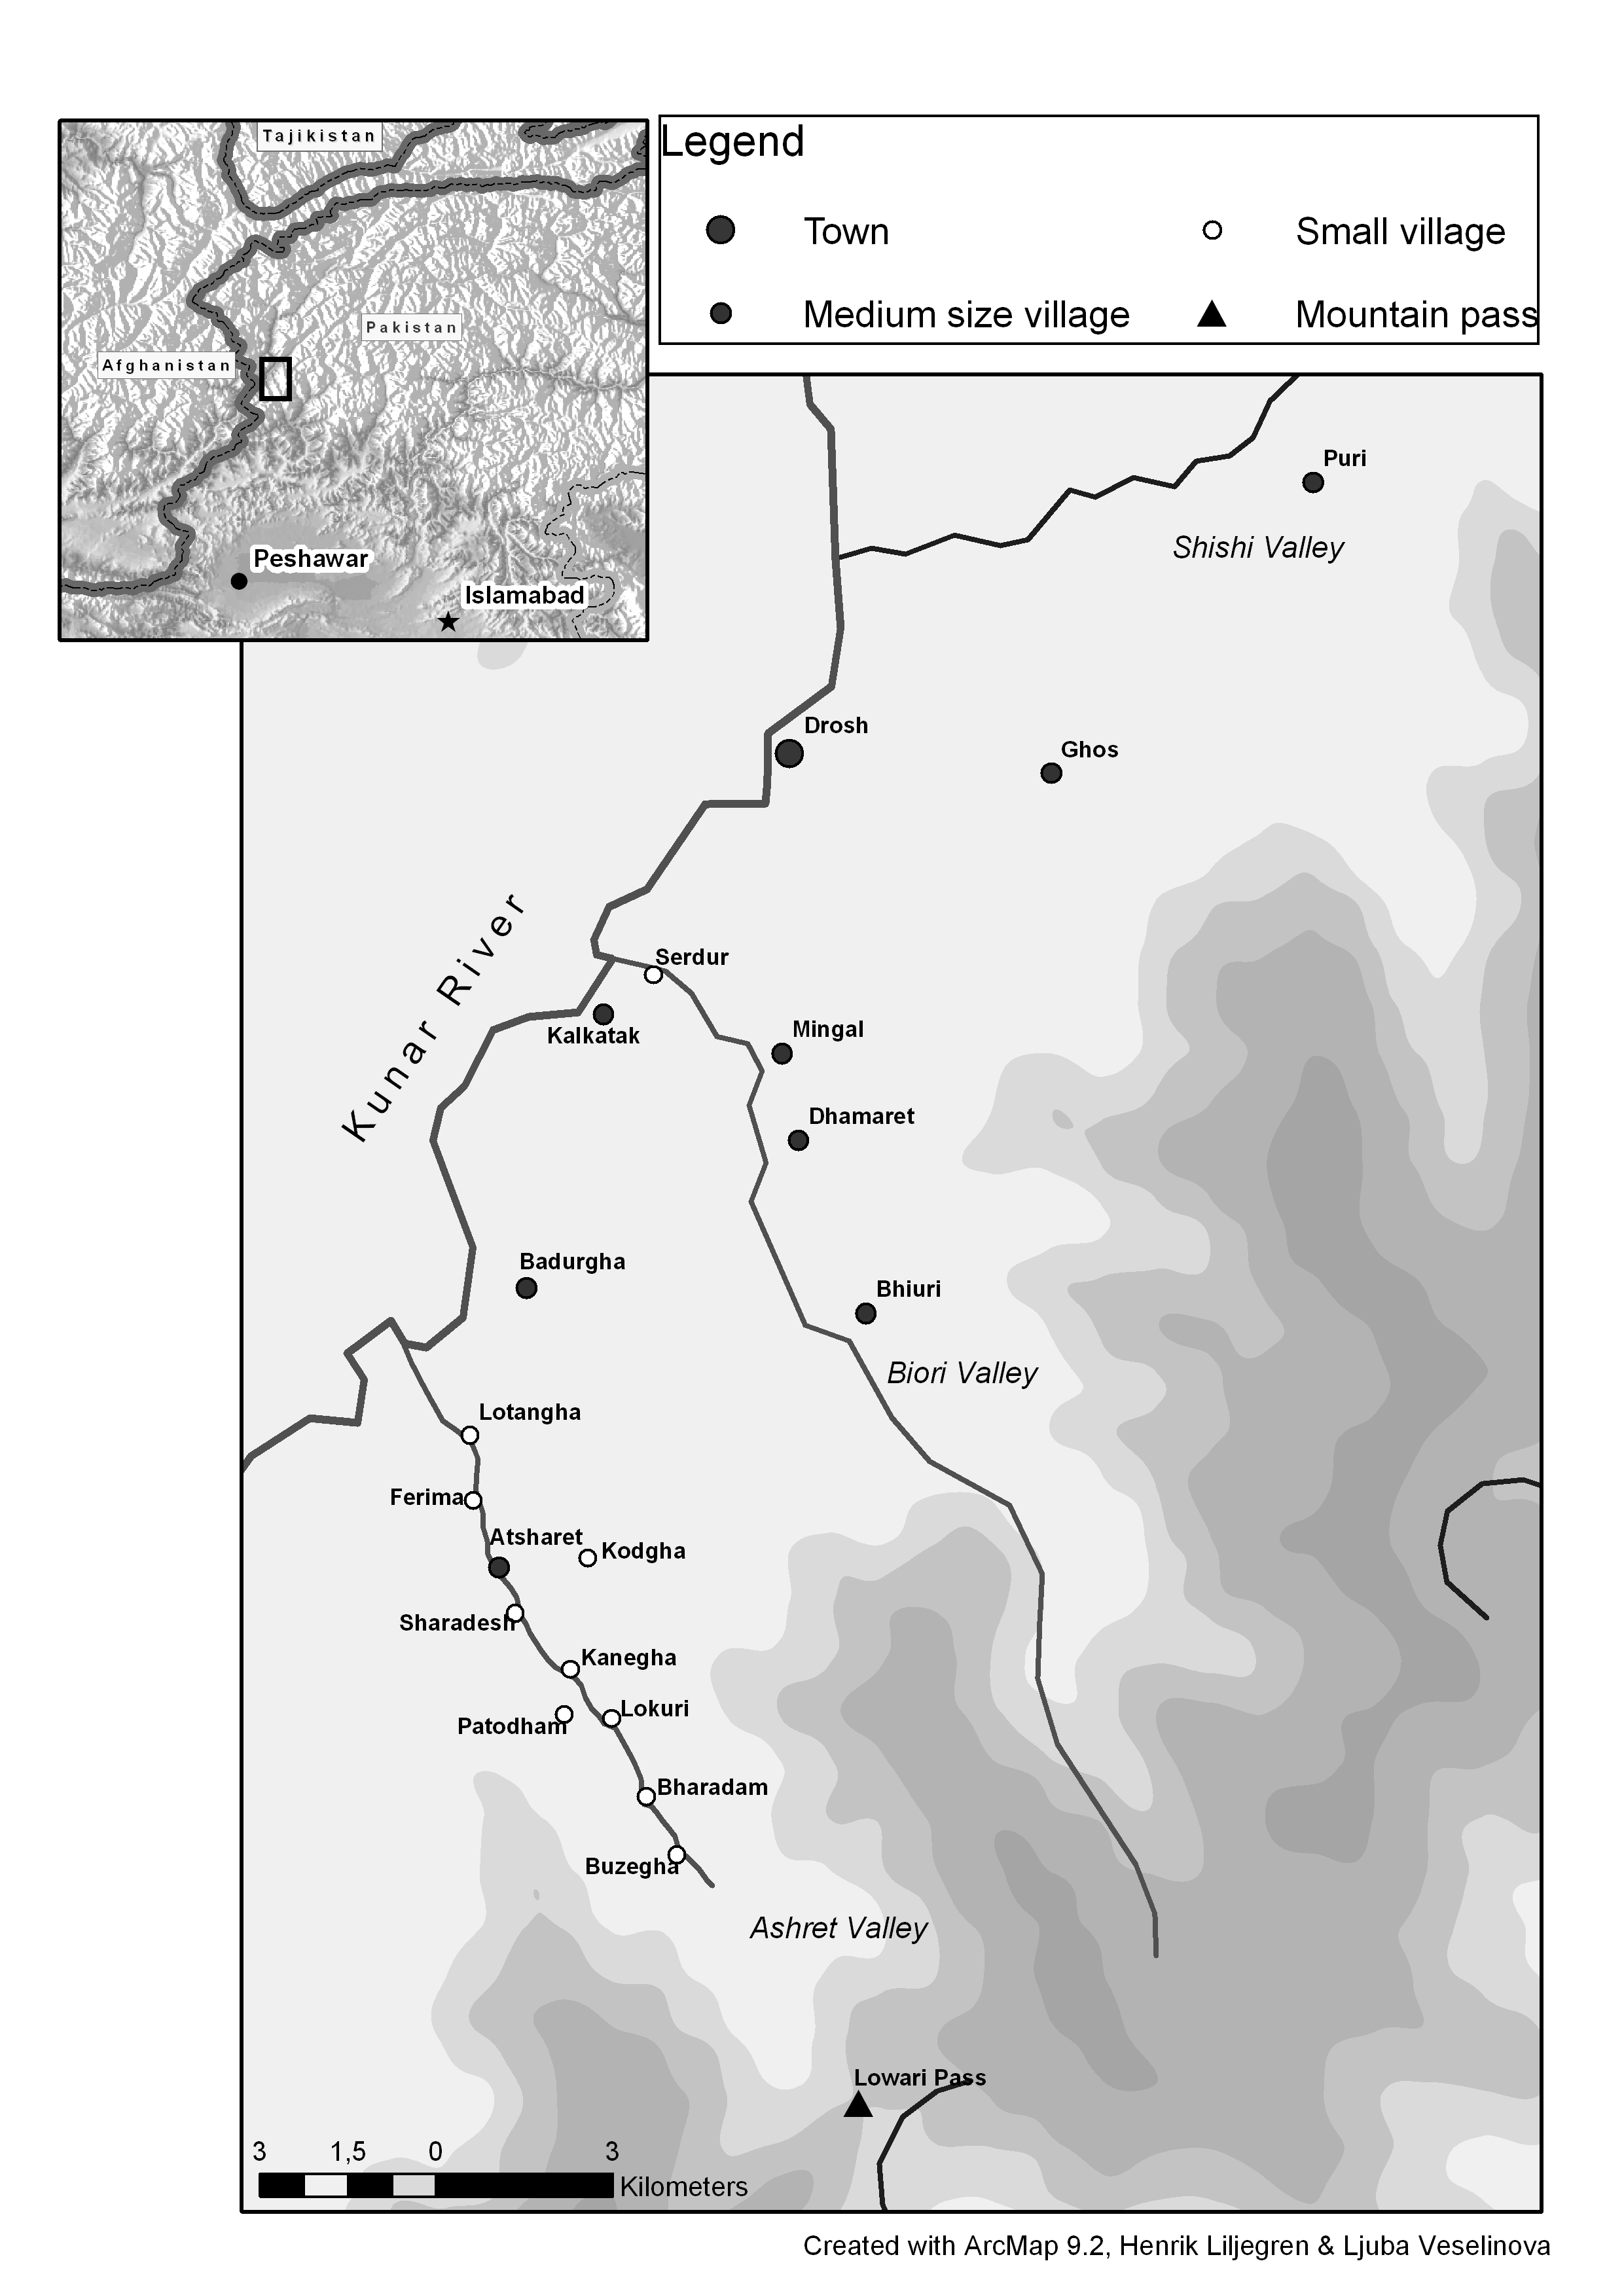
\includegraphics[width=\textwidth]{figures/ch1map1.png}
\edcomm[inline]{Map 1 ist zu lang. Da müsste unten etwas von dem Weißen abgeschnitten werden.}
\label{map:1-1}
\end{mapfigure}


Four kilometres south of the bazaar town Drosh, the Biori Valley meets the main valley along the Kunar river. There are three distinct villages in this narrow side valley, which together with the Ashret Valley is to be considered the heartland of the Palula speaking community, all of them solidly Palula speaking: Mingál (or Lower Biori), Dhamareét (or Middle Biori), and Bhiúuṛi (or Upper Biori/Biori proper), the latter being the largest of the three. 


Apart from those two main settlements, there are a~few other non"=adjacent villages where Palula is or has been spoken in the recent past.


The northernmost of these villages is Purigal (Púri in Palula), which is situated about 20 kilometres north of Drosh, about 7 kilometres into the Shishi Koh Valley. Once an~exclusively Palula"=speaking village, the language is now competing, more than likely on the losing side, with Khowar.


The next location with a~substantial number of Palula speakers~-- though the number is markedly in decline~-- is Kalkatak (Galaṭáak), a~village situated in the fertile main valley, six kilometres by the main road south of Drosh, near the mouth of the Biori Valley. In this village, Palula competes primarily with Khowar, and to a~considerably lesser extent with Pashto, and the usage of Palula is dramatically decreasing in the younger generation. This may in some ways be the repetition of the scenario in this village about a~century ago, when Palula obviously won ground over the then dwindling Kalasha language (\citealt[165]{decker1996}; \citealt[95]{cacopardo2001}). The small village Serdur (Sawdár), situated right at the mouth of Biori Valley, where the majority is reported to speak Palula, is for official purposes treated as a~part of Kalkatak, but it is on the local level mostly considered a~separate unit (Fakhrud Din, pc).


On the arid mountainside a~couple of kilometres east of Drosh is a~small and remote village called Ghos (Ghoós), which apparently was Palula"=speaking in the recent past (\citealt[75, 84]{decker1992a}), but, according to an~informal survey carried out in 2005 by my local language consultants, it has switched entirely to Khowar.


Another village that deserves to be mentioned is Badrugal (Baaḍurghaá), which is located in the main valley between Ashret and Kalkatak, and according to local sources is inhabited by a~substantial number of people able to communicate in Palula. The first language of most (male) villagers is given as Shekhani or Shekhwar, a~Nuristani language, but many have reportedly acquired Palula in frequent contact (especially through intermarriage) with the nearby Palula settlements. 


Outside of what is in a~strict sense part of the Palula"=speaking area in Chitral, one other place
that should be mentioned is a~village called Gumandand (Gumaaṇḍáṇḍ) in Dir Kohistan (in the
neighbouring Upper Dir District to the east). Previously, \citet[9]{morgenstierne1941} mentioned the
tribal connection between this village and the Palula of Chitral, and a~number of people in Ashret
have similarly pointed out that they indeed have relatives there, as a~result of a~past migration
from Ashret. However, I have yet to come across any solid evidence for the same or a~similar
language being spoken there. It is also unclear whether there is a~linguistic or tribal connection
between this village and another village in Dir Kohistan, namely Kalkot, where a~closely"=related
speech variety has been recorded (see \sectref{subsec:1-3-1} for a~discussion on the
relationship between the Palula of Chitral and the speech of Kalkot).


\begin{table}
\caption{Estimated number of Palula (P.) speakers in each location}
\begin{tabularx}{\textwidth}{ l l Q }
\lsptoprule
Location &
 P. speakers &
Comment\\\hline
Ashret Valley &
5,899 &
Pashto"=speaking Buzeeghaa subtracted from a~total of 6071 (2004)\\
Biori Valley &
3,000 &
Approximation based on number of households (2004)\\
Purigal &
\phantom{9}200 &
An estimated 50 per cent of the six to seven people in each of the 60 households (2004)\\
Kalkatak &
\phantom{9}541 &
Speakers counted (1998), includes Serdur\\
Badrugal &
\phantom{9}200 &
Rough estimate\\
\textbf{Total} &
\textbf{9,841} &
\\\lspbottomrule
\end{tabularx}
\label{tab:1-1}
\end{table}


As far as the total number of Palula speakers is concerned, we can only provide a~rough estimate at
best (shown in \tabref{tab:1-1}), due partly to the lack of any reliable census directly mapped
to language use, and partly to the changeable and multilingual situation of the region. Based on
a~combination of population data provided by a~local health network in Ashret, the results of
surveys carried out by the local ethnographer/sociologist Fakhrud Din in Biori and Kalkatak,
interviews with local respondents in Purigal, and an~assumption that there are a~couple hundred
speakers of Palula in Badrugal (out of a~total population of 740 in 1987 according to
\citealt[143]{decker1992a}), we conclude that there are approximately 10,000 speakers of the
language in Chitral, a~figure that should be treated with a~certain amount of healthy
scepticism.\footnote{The seemingly exact figure 8600 that \citep[74--76]{decker1992a} arrived at
  (later cited by Ethnologue) was in fact also the result of quite a~rough estimate, based on
  a~combination of respondent opinion and a 1987 census report.}


Provided there has been no dramatic increase in any of the other speech communities in the district, Palula is still the second largest language community in Chitral, as it was according to a~survey carried out in the 1990s (\citealt[11]{decker1992a}). 

\subsection{The socioeconomic environment}
\label{subsec:1-2-2}

All of the locations with any higher concentration of Palula speakers are villages with a~rudimentary infrastructure. The community at large is agricultural, often combined with animal husbandry, and its inhabitants also receive income from timber harvesting, in the form of royalties on the cedar forest and through the sale of firewood. The main subsistence crops cultivated are wheat and maize, but also a~variety of fruit and vegetables is grown. In most of the villages there is an~ample supply of water for irrigation. 


A portion of the population in the Ashret, as well as in the Biori, Valley practice transhumance, in the spring taking their herds of sheep and goats to the high pastures situated at the extreme ends of these valleys and staying there throughout the summer months. This practice, and interrelated activities such as the production of a~large variety of dairy products, was a~central part of community life and traditions but has given way to today's mainly agricultural society. Whereas irrigated land in and adjacent to the villages and nearby winter pastures are owned by individual families, the distant summer pastures are communal.


As the educational level is steadily increasing and the demand for an~income source besides agriculture is deemed necessary, a~growing number of people are being employed by the government or carry out business within the private sector, either in their home village, e.g. as school teachers, or in the bazaar town Drosh or in Chitral town, the administrative centre of the district. There is also a~local bazaar in Ashret proper, occupying a~smaller number of shopkeepers and craftsmen from the valley. In pursuit of other employment opportunities, a~number of Palula families have migrated to urban areas, settling more or less permanently in larger cities such as Peshawar, Rawalpindi and Lahore.

\subsection{Local history and cultural identity}\label{Local history and cultural identity}
\label{subsec:1-2-3}

Palula has usually been described or seen as a~single"=language community (\citealt[7]{morgenstierne1941} ; \citealt[67]{decker1992a}, \citeyear[160]{decker1996} ; \citealt[21]{masica1991}; \citealt[253, 258]{strand2001}) as well as a~single"=ethnic community \citep[79--143]{cacopardo2001}. Although the former is not very surprising, considering the relatively minor dialectal differences, the latter is a~more complex issue.


From the outsider perspective, and more specifically from the perspective of the Khowar speaking majority of Chitral District, the people and the speech of the Ashret and Biori Valleys are indistinguishable, and they refer to the people as a~whole as the Dangarik and their speech~-- dramatically different from their own language~-- as Dangarikwar. Internally, however, the picture is less clear. Indeed, from the perspective of the ``southerners'' in Ashret, the speech of the ``northerners'' in Biori is rather similar and largely comprehensible, and vice versa, but from both sides the idea is also common that the other variety is a~speech form that is somehow debased or has deteriorated from its pure or original form. Although speakers of the two varieties have interacted and to some extent have also intermarried for a~long time, it is obvious that the community in Ashret do not consider the community in Biori to be related to them, the main reason being that they have no genealogy in common. 


As is the case in many other communities in the region, there are preserved oral traditions concerning a~particular place of origin in these communities as well as genealogies memorised from generation to generation. The most extensive and consistent traditions of this kind is found in Ashret,\footnote{These traditions, including the important historical manuscript Tarikh-i-Ashret, written by the local poet and historian Mirza Guldali Shah in Persian verse, are commented on at great length and in great detail by \citet[79--143]{cacopardo2001}, and a~translation of it into English is included in its entirety as an~appendix to their work.} where the entire population claims descent from a~common ancestor. 


According to local history, the ancestor of the people of Ashret was Choke, son of
Machoke\footnote{In some versions of this tradition, Choke and Machoke were brothers
  (\citealt[85]{cacopardo2001}, and my own notes).}, who migrated to the present location from
Chilas in the Indus Valley some 15 to 16 generations ago, a~scenario convincingly corroborated by
recent research into local history and culture carried out by the anthropologist Alberto Cacopardo
\citep[84--93]{cacopardo2001}. One particular source states how Choke and two of his brothers
arrived in Chitral and reached Drosh but subsequently separated. One brother went to Kalas,
a~village in the Shishi Koh Valley north of Drosh, another continued to Sau in the Kunar Valley (in
present"=day Afghanistan), where he settled, and Choke himself settled in Ashret
\citep[84]{cacopardo2001}. This would support a~common origin of the Palula speakers of Ashret and
the inhabitants of Sau, the language of the latter closely related to Palula.\footnote{This was
  confirmed by respondents from Sau interviewed in an~Afghan refugee camp in Dir in 2000 by Ajmal
  Nuristani and myself who stated that ``the people of Ashret are our brothers''.} The inhabitants
of present"=day Kalas, on the other hand, are all Khowar speakers, but according to respondents in
Puri (the only remaining Palula"=speaking village in Shishi Koh Valley), the people of Kalas formerly
spoke Palula. An independent local tradition among the Bozhokey in the Laspur Valley (about 200 km
northeast of the Palula"=speaking area) also speaks of a~migration from Chilas some 12 to 15
generations ago. Dr. Inayatullah Faizi, himself a~Bozhokey, has documented this tradition, according
to which the two brothers Choke and Machoke left Chilas after a~power struggle with their elder
brother, and after having parted during their exile, Machoke arrived in Laspur where his elder son,
Laphur, subsequently settled. The descendants in the Laspur Valley have since been linguistically
assimilated by their Khowar"=speaking neighbours. Also, some Ashreti sources claim that the Chilasi
immigrants indeed came to Ashret from the north, perhaps via Laspur, rather than through the Lowari
Pass and Dir Kohistan, which would agree with this Laspuri tradition \citep[85, 125--126]{cacopardo2001}.


What then about the Palula speakers in Biori? They are not mentioned in any of the migration
traditions from Ashret (or those agreeing with it), whereas it has been explicitly pointed out to me
by Ashretis that the people of Biori are descendants neither of Choke nor Machoke but are Kohistanis
from Dir who later adopted the language of Ashret (cf. \citealt[255]{strand2001};
\citealt[296]{saeed2001}). The first part of the statement can very well be true, as the main Biori
genealogies lack any convincing links to the genealogies of Ashret, but I suspect the second part to
be an~overinterpretation on the part of the Ashreti informants. Although the ethnic composition of
the Biori Valley population is much more complex (including considerable sections with Kalasha and
Nuristani origin), and with much less consensus around its origin than what is the case in Ashret,
there is indeed a~local tradition that connects a~major section of the population (especially in the
uppermost village Bhiúuṛi) with Dir Kohistan, in particular with a~village called Biyar
(Bhiáaṛ). Although somewhat speculative, it is possible that a~genitive or perhaps an~adjectival
form along with a~regular sound change from ‌/aː / to /uː/ would render the form Bhiúuṛi,
i.e. ``from Biyar''. Also \citet[111--108]{cacopardo2001} draws the conclusion that the
Palula\footnote{Keeping in mind that the ancestors of a~good portion of the ethnically"=mixed
  population most likely were speakers of a~variety of Kalasha, and that there may also have been
  other linguistic enclaves before Palula became the sole surviving language of the valley.} of
Biori most likely came to the valley from Dir Kohistan, somewhat later than the Palula of Ashret,
possibly to escape conversion to Islam, which was common at the time in Dir Kohistan. While
present"=day Biyar is a~Kohistani (Gawri"=speaking) village, and there are no obvious traces of any
previous language spoken in the village, it is not wholly unlikely that the population speaking
a~language closely related to Palula in the relatively close village Kalkot (both being situated
along the Panjkora river) is a~remnant of a~once more widely spoken Shina variety in this part of
Dir Kohistan. Atiq Ullah, a~local historian and also my main language consultant in Biori, further
claims that the people who came from Biyar were originally from Tangir, one of the Indus side
valleys west of Chilas (hence the name Tangiri/Dangarik as mentioned
earlier).\footnote{Interestingly, while Ashreti people usually dislike the Chitrali designation
  Dangarik or Dangarikwar, the people of Biori do not seem to mind and sometimes even use the term
  referring to their own community.} In Puri (also part of the same general dialect area as Biori),
a~local elder told me that their village was founded by two brothers, Dúuši‌ and ‌Kaṇúuši, who came
via Dogdarra, a~valley in Dir Kohistan, from a~village in the Tangir Valley called Dangeri Phuruṛi,
possibly corresponding to a~very real place in central Tangir that is rendered Phurori on some
maps. As a~possible explanation for the exclusiveness on the part of the Ashretis vis-à-vis the
Palula speakers of Biori, Inayatullah Faizi (pc) has suggested that those ancestors of the Biori
Palula who came from Dir Kohistan may very well have been Shina speakers, but being Yeshkun rather
than Shin\footnote{According to \citet[17]{jettmar2002}, the population in the traditional Shina
  territory was organised into four castes~-- Shins, Yeshkuns, Kamins and Doms~-- with the Shins
  considering themselves ritually cleaner than the other three, possibly modelled on Hindu
  communities in adjacent areas. } would immediately have placed them in a~non"=kin category,
regardless of the their linguistic relatedness.\footnote{This idea, however, is disputed by Alberto
  Cacopardo (pc), who holds that the awareness of such a~caste identity in relatively recent times
  is out of question.}


What this gives us are (at least) two possible migration routes from the Indus Valley to
Chitral. One would have originated in the Chilas area, in the main Indus Valley, taking the way over
the Shandur Pass to Laspur and then continuing south through Chitral to the Ashret Valley, branching
out quite early on to Sau in the Kunar Valley. The other one would have originated in the Tangir
Valley,\footnote{As rightly pointed out by Alberto Cacopardo (pc), there is a~narrow, modern"=day use
  of Tangir that refers to a~particular side valley to the west of Chilas in the Indus Valley, but
  there is also a~broader, past use of Tangir that refers to the larger region around Chilas,
  including many of the major areas where varieties of Shina are spoken.} taking the route over
Swat/Dir Kohistan, leaving a~trace in Kalkoti speech, and ending up in the Biori Valley. Whether or
not there is any linguistic evidence supporting this hypothesis is something we will have reason to
return to briefly below (\sectref{subsec:1-3-1}).


The arrival of the Palula in Ashret must, if the local genealogical evidence and other historical
traditions are taken into account, be dated to some time before the mid-17\textsuperscript{th}
century \citep[88]{cacopardo2001}, and the migration from Dir Kohistan to Biori somewhat later
(\citeyear[118]{cacopardo2001}). As for the religion of the Palula speakers, they were clearly still
unconverted to Islam when they first entered Chitral, and it was probably not until the latter half
of the 19\textsuperscript{th} century when they embraced Islam (\citeyear[83]{cacopardo2001}), and
even then only gradually and probably earlier in Ashret than in Biori. What kind of religion was
practiced before the Muslim conversion remains uncertain, but elements in it are shared with the
non"=Islamic Kalasha as well as what is known about other pre"=Islamic religions in the region.


Finally, I will quote Alberto Cacopardo's brief but interesting summary of his own findings about the great"=grandfathers of today's Palula:

\begin{quote}
They were goat"=herders, whose women in the summer watered the fields, while the men went up on their
own to the high pastures. Cows were impure to them, like the women at the time of seclusion. They
had something like a~priestly lineage, and some of them held feasts of merit. They lived in densely
forested valleys haunted by murderous bandits and by the fear of monstrous ghosts. They were mostly
dressed in goatskins and travelled only on foot, but they remembered ancestors who rode on horses
and fought with bows and arrows against princes who lived in forts. They had rites in which they
drank wine and men and women danced together at night. They had temples and shrines, sacred stones
and wooden idols, and they said they heard the voices of the fairies \citep[143]{cacopardo2001}.
\end{quote}

\section{The linguistic setting}
\label{sec:1-3}
\subsection{Genetic affiliation}
\label{subsec:1-3-1}
Palula belongs to a~group of IA languages spoken in the Hindu Kush region that are often referred to as ``Dardic'' languages. It has been and is still disputed to what extent this primarily geographically defined grouping has any real classificatory validity.\footnote{For an~overview of the terms Dard, Dardic and Dardistan and their different uses, see \citealt{mock1997}.} On the one hand, \citet[251]{strand2001} suggests that the term should be discarded altogether, holding that there is no justification whatsoever for any such grouping (in addition to the term itself having a~problematic history of use), and prefers to make a~finer classification of these languages into smaller genetic groups directly under the Indo"=Aryan heading, a~classification we shall return to shortly. 

\begin{mapfigure}[p!]
\caption{Languages in the Hindu Kush region}
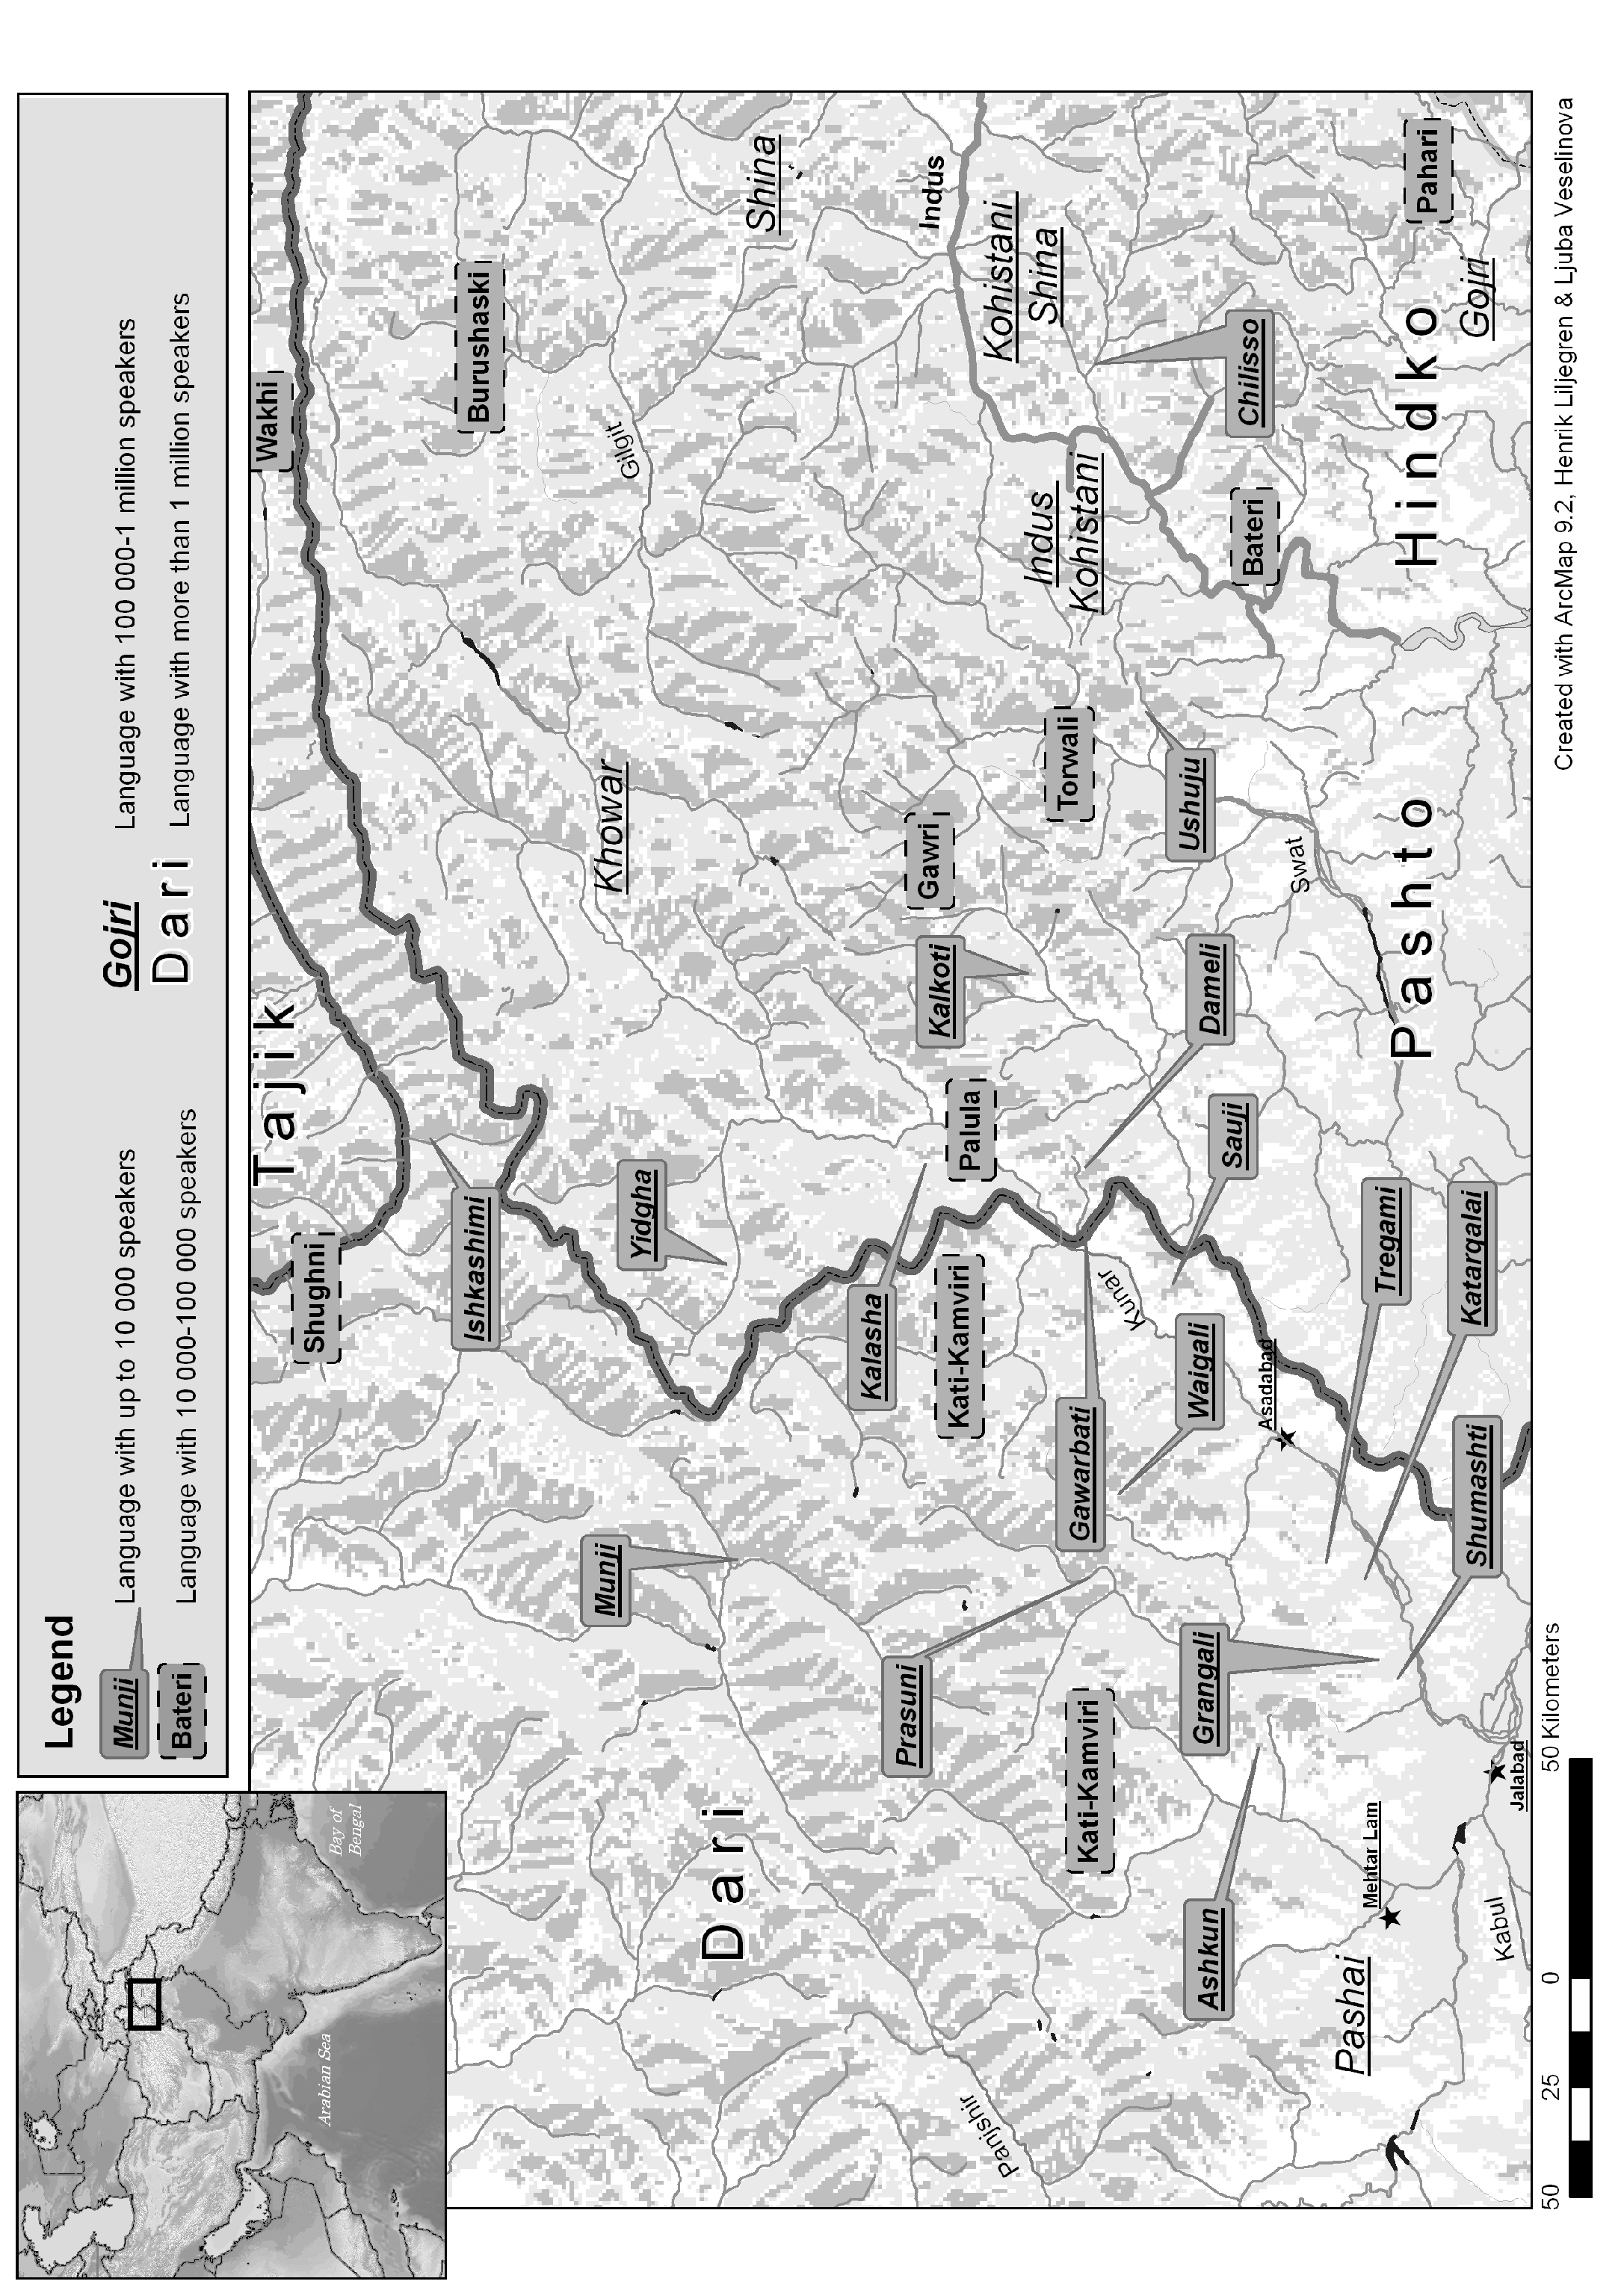
\includegraphics[width=\textwidth]{figures/ch1map2.png}
\edcomm[inline]{Map 2 sollte vielleicht ein Querbild sein?}
\label{map:1-2}
\end{mapfigure}

Others have continued using the term, for various reasons, in a~classificatory sense. \citet[822]{bashir2003} concludes that there are enough similarities across these languges, in terms of shared retentions, areal features and innovations affecting at least subsets of the languages to justify the umbrella term ``Dardic'' even though she expresses doubt about the possibility of tracing them all to a~single node in a~Stammbaum model. \citet[10--11]{zoller2005} identifies the Dardic languages as the modern successors of the Middle Indo"=Aryan (MIA) language Gandhari (also Gandhari Prakrit), but along with Bashir, Zoller concludes that the family tree model alone will not explain all the historical developments. 


\citet[460]{masica1991} questions the value of trying to sort out a~complete and accurate New Indo"=Aryan (NIA) historical taxonomy and contends that it would be far more interesting to focus on and recognise a~number of overlapping genetic zones, some of them more strongly defined than others. Following that position, I will in the remainder of this work refer to these languages as Hindu Kush Indo"=Aryan languages (HKIA), without any claim of taxonomical correctness but recognising the shared historical developments pointed out by Bashir and Zoller. 


Some words should now be said about the lower"=level grouping of these HKIA languages, which have as their home an~extremely mountainous region that stretches from north"=eastern Afghanistan over northern Pakistan all the way to Kashmir (see Map~\ref{map:1-2}). \citeauthor{strand2001} recognises in his classification (\citeyear[258]{strand2001}, which represents an~updated and corrected version of \citealt{strand1973}) eight groups (some of them represented by one language alone): 

\begin{enumerate}
\item \textit{Pashai}, with a~western and an~eastern dialect cluster, is spoken in an~area north of Kabul River in Afghanistan, close to the Pakistani border. 


\item \textit{Pech group} includes the languages Gawarbati, Grangali and Shumashti, of which the latter two are seriously threatened. Grangali and Shumashti are spoken in the same general area as Pashai, and Gawarbati is spoken in the Kunar Valley on both sides of the Afghan"=Pakistan border. 


\item \textit{Pech"=Kunar group}, which as a~group is merely hypothetical, consists of one known language, Katarqalai, perhaps still spoken in one single village in the lower Tregam Valley, not far from the main Kunar Valley in Afghanistan. \citet[825]{bashir2003} places it in the Kohistani group.


\item \textit{Chitral group}, with its two languages Khowar and Kalasha, which are both spoken in Chitral District in Pakistan.


\item \textit{Tirahi}, which is perhaps no longer extant, was the language of a~few villages southeast of Jalalabad in Afghanistan. \citet[824]{bashir2003} places this language in the Kohistani group.


\item \textit{Kohistani group}, includes a~number of rather diverse languages at the centre of the HKIA region. Strand places Dir/Kalam Kohistani (or Gawri) and Dameli\footnote{An entirely accurate classification is still lacking.\citet[824]{bashir2003}, for instance, groups Dameli with Gawarbati in a~Kunar group.} in a~western cluster, the former spoken in Dir/Swat Kohistan and the latter in southern Chitral. In an~eastern cluster we find Indus Kohistani, Gowro, Chilisso and Bateri, all spoken in the Indus Valley, and Torwali in upper Swat.


\item \textit{Kashmiri}, with its two main dialects Kashtawari and Poguli, is spoken in Kashmir. 


\item \textit{Shina}, where the closest relatives to Palula are found, is traditionally described as one language with different dialects, but in actual fact it covers a~number of rather diverse and geographically widespread varieties, spoken by a~range of ethnic groups, from the Kunar Valley in Afghanistan all the way to Kashmir (with its largest uninterrupted area along the portion of the Indus stretching from Kohistan district in the south, through Chilas District, covering the east"=west flowing portion of the river, then in the Northern Areas branching out both eastwards into the Skardu area of Baltistan and westward along the Gilgit River). Strand identifies two main clusters, a~Chilasi cluster and a~Gilgiti one:

\begin{tabbing}
Chil\=Kohistanddi\=\kill
Chilasi \\
\>Kohistani Shina \\
\>Eastern dialects \\
\>\>Astori \\
\>\>Drasi \\
\>Dispersed dialects \\
\>\>Palula \\
\>\>Ushuju (?) \\
\>\>Kalkoti (?) \\
Gilgiti \\
\>Brokskat (a Tibetanised offshoot) \\
\end{tabbing}

\end{enumerate}

Strand further identifies the dispersed and archaic varieties Palula and Sawi (or Sauji) as of particular interest (the reason he does not include Sawi in the list is perhaps that he sees Palula and Sawi as basically one and the same variety), and that two other speech enclaves, Ushuju and Kalkoti, probably should be included as well.


It is primarily in a~phonological comparison between cognates that Palula appears to be conservative vis-à-vis the other Shina varieties (\tabref{tab:1-2}). In a~comparative study between some major varieties (Palula not included), \citet[36]{schmidt2002} shows that three features are common to all of them: a) the preservation of the OIA three sibilants \textit{s, š, ṣ}, as in HKIA languages at large, b) the development of retracted (retroflex) fricatives \textit{c̣} and \textit{ẓ} from OIA clusters \textit{tr, kṣ, dr, bhr,} etc., and c) the development of contrastive pitch accent. 


While Palula shares the first and the third of those with the other varieties, it has to a~larger extent preserved consonant clusters. 


\begin{table}[ht]
\caption{Comparison of cognates in five Shina varieties (based on \citealt[37]{schmidt2002}, with Palula (A.) data added)}
\begin{tabularx}{\textwidth}{ l l X l X l l }
\lsptoprule
OIA &
Gilgiti &
Kohi\-stani &
Drasi &
Brok\-skat &
Palula &
\\\hline
\textit{ɡōṣṭá-} &
\textit{ɡoóṭ} &
\textit{ɡóoṣ} &
\textit{ɡoóṣ} &
\textit{ɡoóṣ} &
\textit{ɡhoóṣṭ} &
`house'\\
\textit{kr̥ṣṇá-} &
\textit{kíno} &
\textit{kíṇo} &
\textit{kíṇo} &
\textit{kyóno} &
\textit{kriṣíṇu} &
`black'\\
\textit{kárman-} &
\textit{kom} &
\textit{kom} &
\textit{krom} &
\textit{krum} &
\textit{kráam} &
`work'\\
\textit{kṣ\'{\={e}}tra-} &
\textit{c̣héec̣} &
-- &
\textit{c̣héec̣} &
-- &
\textit{c̣híitr} &
`field'\\
\textit{bhr\'{\={a}}tr̥-} &
\textit{ẓáa} &
\textit{ẓáa} &
\textit{ẓáa} &
-- &
\textit{bhroó} &
`brother'\\
\textit{*ǰāmātra-} &
\textit{ǰamac̣oó} &
\textit{ǰamc̣ó} &
\textit{ǰamac̣oó} &
\textit{ǰamó} &
\textit{ǰhamatroó} &
`son"=in"=law'\\
\textit{divasá} &
\textit{déez} &
\textit{dées} &
\textit{dées} &
\textit{dis} &
\textit{deés} &
`day'\\\lspbottomrule
\end{tabularx}
\label{tab:1-2}
\end{table}


Something should be said about two of the other so"=called ``dispersed dialects'', Sawi/Sauji and Kalkoti, and their relationship to Palula. 


\textit{Sauji} (the form used by my respondents when referring to their language in contrast to
Sawi, which is the way it has been referred to in most literature) is the speech variety of Sau,
a~village situated on the east bank of the Kunar River in Afghanistan, about 20 kilometers south of
the Pakistani border town Arandu in southern Chitral. It is uncertain to what degree and by how many
people Sauji is spoken today in this village, but according to \citeauthor{decker1992a}'s
(\citeyear{decker1992a}) informants, approximately 8,000--12,000 lived in the village prior to the
long period of war and unrest in Afghanistan.\footnote{A good portion of a~refugee camp in Timargira
  in district Dir that I visited along with Ajmal Nuristani in 2000 was made up of Sauji"=speakers
  from Sau. However, in the last few years many are said to have returned to their home village in
  Afghanistan.} That the variety spoken in Sau is closely related to Palula was pointed out
previously by Morgenstierne in the first half of the last century \citep[7]{morgenstierne1941}, and
was further confirmed by the more extensive study of the language undertaken by Buddruss in the
1950s:

\begin{quote}
Dagegen ist die nahe Verwandtschaft des Sawi mit dem Phal. bereits durch einen Blick in Grammatik und Vokabular evident und wird überdies durch die Angabe meines Gewährsmannes bestätigt, daß er die Sprache der Leute von Ashret verstehen könne. Dennoch sind die beiden Sprachen keineswegs identisch mit einander. \citep[11]{buddruss1967}
\end{quote}


That there is a~historical connection between Sau and Ashret according to local tradition was
already mentioned (see \sectref{subsec:1-2-3}), but no major interaction or
contact between the two communities seems to have taken place in the recent past, and for a~long
time, the population of Sau has been included and been seen as a~part of the all"=surrounding Gawar
community, sharing their identity in all aspects save the language, something rather remarkable from
a~regional perspective \citep[232]{cacopardo2001}.


\textit{Kalkoti} (or Khalkoti), on the other hand, has remained largely undocumented. It is spoken by approximately 6,000 people, apparently confined to a~village called Kalkot, situated in the upper Panjkora Valley in Dir Kohistan. Since no systematic survey has been carried out in Dir Kohistan, however, it is too early to exclude the existence of other locations where this variety or something similar is spoken. Most other villages in the main valley, from Rajkot (Patrak) and upstream, are Gawri"=speaking,\footnote{I use Gawri to refer to the Kohistani varieties that have been variously called Bashkarik, Kalam (Kalami) Kohistani or Dir Kohistani. Gawri seems to be the preferred name and one that can be accepted by speakers from locations both in Swat and Dir Kohistan.} but that the speech of this village\footnote{In fact, about 70 per cent of the Kalkot population are speakers of Kalkoti, whereas the remaining 30 per cent are speakers of a~Gawri variety (Muhammad Zaman Sager, pc).} could be something rather different was first hinted at in a~sociolinguistic survey carried out by \citet[7]{rensch1992} and his colleagues: ``The linguistic variety spoken in the village of Kalkot in Dir Kohistan seems to be quite distinct from that spoken in the surrounding villages of Dir Kohistan and in Kalam, although it is obviously related''. Richard Strand, as was pointed out above, tentatively classified Kalkoti as a~Shina variety closely related to Palula, based on the word list presented in the already mentioned survey report \citep[159--176]{rensch1992}, particularly pointing to the strikingly similar forms of the personal pronouns. Perhaps there is, as was mentioned above (\sectref{subsec:1-2-3}), a~historical connection between the Palula speakers of Biori, who tradition says came from Dir Kohistan, and the Kalkotis.


My own study, based on data collected by Naseem Haider and Muhammad Zaman Sager in Kalkot in early 2006, confirms the hypothesis that Palula and Kalkot are closely related and also that Kalkoti, although heavily influenced by Kohistani (Gawri), is essentially a~Shina variety. The assumption is that certain types of words (see \tabref{tab:1-3}) are much less likely to be borrowed, such as personal pronouns, lower numerals, kinship terms, and basic verbs \citep[23]{trask1996}.


Based on this, it seems that the two main Palula dialects, Sauji and Kalkoti, although separated for perhaps several centuries, form some sort of cluster of their own.


\begin{table}[ht]
\caption{Lexical comparison between Palula (A. variety), Kalkoti and Gawri}
\begin{tabularx}{\textwidth}{ Q Q Q Q }
\lsptoprule
Palula (A.) &
Kalkoti &
Gawri &
\\\hline
\textit{ma} &
\textit{ma} &
\textit{yä} &
`I'\\
\textit{be} &
\textit{bä} &
\textit{mä} &
`we'\\
\textit{tróo} &
\textit{traa} &
\textit{ɬää/‌ɬaa} &
`three'\\
\textit{akóoš} &
\textit{akaaš} &
\textit{ikää} &
`eleven'\\
\textit{bóoš} &
\textit{baaš} &
\textit{bää} &
`twelve'\\
\textit{baábu} &
\textit{bab} &
\textit{bob} &
`father'\\
\textit{yéey} &
\textit{yi} &
\textit{yeey} &
`mother'\\
\textit{brhoó} &
\textit{draa} &
\textit{ǰää} &
`brother'\\
\textit{bheéṇ} &
\textit{bään} &
\textit{išpo} &
`sister'\\
\textit{šúur} &
\textit{šur} &
\textit{šušur} &
`father"=in"=law'\\
\textit{preṣ} &
\textit{irpäṣ} &
\textit{čiš} &
`mother"=in"=law'\\
\textit{hínu (de)} &
\textit{in (aas)} &
\textit{thu (aaš)} &
`be'\\
\textit{biáanu (ɡúum)} &
\textit{buun (ɡu)} &
\textit{bäčant (ɡaa)} &
`go'\\
\textit{bháanu (bhílu)} &
\textit{buun (bil)} &
\textit{hoant (hu)} &
`become'\\
\textit{tháanu (thíilu)} &
\textit{thuun (thääl)} &
\textit{kärant (kiir)} &
`do'\\\lspbottomrule
\end{tabularx}
\label{tab:1-3}
\end{table}


So far nothing has been said about Ushuju, one of the other ``enclaves'' mentioned by Strand. Not much was known about this language or its speakers prior to the sociolinguistic survey referred to above (\citealt{decker1992}). Ushuju is spoken by an~estimated 2,000 people in the Bishigram Valley in Swat, and the ancestors of the present"=day speakers are said to have migrated from Kolai, a~Shina speaking area in Indus Kohistan (\citealt[69]{decker1992}), and the word list and other data\footnote{Such as the ``core'' verbs \textit{han-/as-} `be' and \textit{th-} `do' (\citealt[ 71--72, 199--203]{decker1992}), which are typical features of Shina.} suggest that it is at its core another dispersed Shina variety (cf. \citealt[255]{strand2001}), although \citet[9]{zoller2005}, without further justifying it, refers to it as ``a Kohistani language with Shina elements''. In any case, the preliminary lexical comparison made by Sandra~\citet[70]{decker1992} did not show any greater similarities with Palula or Kalkoti than with any other Shina varieties, rather the other way around, and there is nothing really that would directly connect the Ushuju community and its migration routes with the Palula"=Sauji"=Kalkoti cluster.


Outside this particular cluster, there are indications that it is the Kohistani Shina subvarieties spoken in the Tangir and Darel Valleys, in today's Diamer district, that may be most similar to Palula \citep[142--143]{radloff1992}. 


\subsection{Areal affinities}
\label{subsec:1-3-2}

There are of course other factors beside genetic relatedness responsible for similarities between languages, one being contact. When looking at the Hindu Kush region where Palula is spoken, one finds a~highly interesting and relatively little researched region, areally as well as linguistically, which lies at the crossroads between different geographical as well as cultural zones. 


From the larger perspective, the region is part of (although at the fringe of) the Indian Subcontinent, and since there are many more languages beside the Indo"=Aryan in the area, many with even longer histories, the question of a~linguistic area or a \textit{Sprachbund} in South Asia becomes relevant. Besides the IA languages, there are other Indo"=European languages, mainly Iranian languages in the west, as well as English (although it has a~relatively short history in the region). In addition to Indo"=European languages, there are representatives of Tibeto"=Burman in the far north and east, Dravidian in the south (with the `remnant' Brahui in the north"=west), Austro"=Asiatic in the northeast, the isolate Burushaski in the northwest, and even Turkic languages in the northwest, although the latter are found outside of what is normally seen as part of the Subcontinent. 


A number of traits (such as retroflex consonants and dative subjects) have been suggested as areal, shared across languages and language families in South Asia, but not without lengthy discussions about what really should be considered areal \citep{emeneau1965,emeneau1980,masica1976,masica1991,masica2001,ebert2006}.


According to \citet{masica2001}, areal traits or features are not only of one kind, which is why he suggests a~finer differentiation between 1) \textit{essentially areal features}, which would be those features really defining the language area (as, for example, the above mentioned ones); 2) \textit{macroareal features}, for features found not only in South Asia, but in most parts of mainland Asia (such as SOV word order); 3) \textit{marginal} or \textit{linking features}, for features ``spilling over'' from adjacent areas but not necessarily affecting the entire South Asia (such as the ``essentially'' Southeast Asian use of numeral classifiers in the northeast, or ergativity linking together South Asia with areas of Western Asia); and 4) \textit{subareal features}, for features defining a~smaller area within South Asia.


Others \citep{dahl2001,ktammwaelchli2001} have been skeptical towards the notion of linguistic areas as such, questioning whether such areas have a~reality of their own rather than merely being convenient ways of summarising certain phenomena. 


Regardless of the particular view one takes on areality in the end, there is reason to further inspect the languages and traits found in the northwestern corner of the Subcontinent (i.e. the Hindu Kush region) ``where conflicting areal patterns meet and interact, and many peculiar languages (`Dardic', Burushaski,\footnote{A language isolate, spoken in a~few valleys in the extreme north of Pakistan.} the Pamir group of Eastern Iranian), at once archaic and innovating, find their home'' \citep[225]{masica2001}. To this collection of languages should be added the Tibeto"=Burman language Balti, which is spoken in the eastern part of the region adjacent to the main Shina belt, and the Nuristani languages, mainly found in the part of Afghanistan bordering Chitral and, to a~lesser extent, on the Pakistani side of the border. The latter were initially lumped together with the ``Dardic'' languages but are now considered a~branch of Indo"=Iranian, beside Indo"=Aryan and Iranian.


A few other scholars of South Asian languages, in addition to those mentioned, have identified features or a~certain convergence of features that seem to be of particular relevance to this region (or some similarly defined region). Some of the more promising are those suggested by \citet{bashir2003}, including grammaticalisation of evidentiality, multi"=differentiating deictic systems, predominantly left"=branching structures, contrasts between dental, retroflex and palatal sibilants and affricates, and the development of tonal/accentual systems, the latter feature further elaborated upon by \citet[132--144]{baart2003}. An interesting feature, only affecting a~few (mostly adjacent but not closely"=related languages) in this subregion, is the development of retroflex vowels, described by \citet{morch1997}. 


The loss of gender distinctions in the geographically"=peripheral Indo"=Aryan language Khowar (and also in closely"=related Kalasha) was pointed out already by \citet{emeneau1965} as resulting from Persian influence (via the Iranian Pamir languages). More research may reveal whether Emeneau's conclusion is correct, and also how this phenomenon is related to an~assumed grammaticalisation of animacy distinctions, present not only in Khowar and Kalasha \citep[401]{bashir1988}, but also in largely undocumented and not yet fully classified Dameli (Emil Perder, pc). Possible substratal influence, related to the isolate Burushaski or other now extinct languages, is also to a~large extent \textit{terra incognita}.


\subsection{``Next"=door'' linguistic neighbours}
\label{subsec:1-3-3}

Surveying the languages of the region in the 1920s, \citeauthor{morgenstierne1941} stated that ``Lower Chitral is one of the most polyglott [\textit{sic}] regions of Asia'' (\citeyear[7]{morgenstierne1941}), and if something characterises the immediate surroundings of the Palula area, it is multilingualism and an~ample opportunity for cross"=language interaction. \citet[10--23]{decker1992a}, in his and his team's sociolinguistic survey, identified as many as 12 languages native to the 200,000+ population of Chitral District at the time, and another four non"=native languages that played some role in the lives of people in the district. 


Some of the nearest linguistic neighbours of the Palula~-- historically or presently~-- are the following:


\textbf{Khowar.}\edcomm{Hier sind die Sprachnamen im ursprünglichen Dokument einfach nur fett markiert. Soll es so bleiben oder als Spitzmarke gesetzt werden?} Although not spoken in any area immediately adjacent to Palula until quite recently, Khowar is now the overall dominant one in the district. It is spoken as the first language of approximately 82 per cent of the population (\citealt[11]{decker1992a}), and functions very much as a \textit{lingua franca}, but in competition with Pashto south of Drosh Bazaar. Khowar is an~IA language classified as belonging to the Chitral group (see \sectref{subsec:1-3-1}). The historical heartland of Khowar and the Kho people is the northern part of the Chitral district, north of Chitral town, from where the language apparently expanded southward to incorporate a~number of other ethno"=linguistically distinct groups that previously used their own languages.


\textbf{Kalasha} is the language spoken by and most intimately associated with the only surviving non"=Muslim population in the entire region. The language is today the first language of 3,000 to 6,000 individuals (\citealt[xi]{trailcooper1999}; \citealt[8]{heegardpetersen2006}) in a~few famous side valleys~-- Birir, Bumboret and Rumbur~-- to the west of the Kunar River, near the Afghan border, and it also includes a~slightly different variety used in Urtsun Valley (where the speakers are Muslim). Due to the unique features of the traditional Kalasha religion and culture, it has received a~great deal of attention from anthropologists and folklorists throughout the years and is therefore probably one of the best documented communities of the region. The Kalasha language was once spoken in a~much larger area~-- corresponding to the local political power held by the Kalasha in earlier times \citep[33]{siiger1956} -- possibly the only language truly indigenous to southern Chitral \citep{strand2001}. The language shares a~number of features with Khowar, linguistically its nearest relative in the Chitral group. Although not spoken in any location adjacent to Palula today, it was probably the closest linguistic neighbour of Palula for centuries, sometimes spoken side by side in the very same location (particularly in Kalkatak and the Biori Valley).


\textbf{Dameli} is spoken by about 5,000 people (\citealt{decker1992a}) in 11 small villages in the Damel Valley, the next populated side valley south of the Palula"=speaking Ashret Valley. Classification has proved to be a~complicated issue with this language, as it shares much lexical and phonological material with Nuristani languages at the same time being similar in most respects to other IA languages in the region. Even though the last word has most certainly not been said about Dameli classification, the tentative conclusion at the time is that it belongs to the Kohistani Group of IA languages \citep[258]{strand2001}, while in certain respects being strongly influenced by neighbouring Nuristani languages. The dominant second language in the Damel Valley is Pashto and all men in the valley are reported to be able to communicate in that language, whereas most women in the valley seem to be monolingual in Dameli (\citealt{decker1992a}). Its position as the primary language for in"=group communication is largely unthreatened. Although there is some intermarriage between Dameli and Palula, the contact between the two groups may have been more frequent in the past, as indicated by shared vocabulary (Emil Perder, pc).


\textbf{Shekhani}, or Kamviri, is a~northern Nuristani language. From its old heartland around Kamdesh in southern Bashgal Valley in Afghanistan, the language had already found its way into Chitral by the end of the 19th century. There are approximately 1,500 to 2,000 speakers of this language (\citealt{decker1992a}) in the villages Langorbat and Badrugal, the latter situated along the main road between the mouths of the Biori and Ashret Valleys, while about 4,000 speakers of the language remain in the old heartland in Afghanistan. The most widespread second language of Shekhani speakers is beyond a~doubt Pashto, a~language preferred even in interaction with Khowar speakers, but (as mentioned above) in Badrugal, Palula seems to have a~rather strong position as a~second (or possibly third) language, apparently resulting from intermarriage with Palula"=speaking families in nearby Palula locations.


\textbf{Pashto}. In spite of its current dominant position as a~trade language and the unrivalled lingua franca of the entire province,\footnote{Pashto is an~Iranian language with a~total of 20 million speakers on both sides of the Pakistan"=Afghanistan border.} Pashto has a~fairly short history in Chitral. Many of those families who now count Chitral as their home district started moving into Chitral in the 1930s. Although no more than 3,000 (\citealt{decker1992a}) individuals in Chitral had Pashto as their first language in the beginning of the 1990s (a figure that more than likely has increased a~great deal), the Pashtuns (or Pathans as they are often referred to) is a~very influential group and, according to one report, control 85 per cent of all trade in the district. While earlier immigrating Pashtuns learnt to speak Khowar in order to carry out their trade, it is now common for speakers of other languages to learn Pashto to have access to trade in Chitral. The largest concentration of Pashto speakers is probably in and around Drosh and along the Kunar River southwards from there. There are also Pashtun settlements in the upper parts of the Ashret Valley. 


\subsection{Patterns of language use}
\label{subsec:1-3-4}

Palula is almost exclusively used among people who speak Palula as their first language. Within the Biori and Ashret Valleys, it is in most cases the only language in communicative use, and there are very few native speakers of other languages residing in those locations. However, as soon as there is a~non"=Palula speaker present, even in one of the main Palula villages, the language switches to one of wider communication, vz. Khowar with most other"=tongue speakers from within Chitral and Pashto, which is used with some non"=Khowar speakers from within Chitral, as well as with Pashtuns from places beyond the Lowari Pass.\footnote{Communication with other outsiders is still rather infrequent, but Urdu would be the natural choice of language to the extent the Palula speaker is able to communicate in it (which constituted about 50 per cent of \citeauthor{decker1992a}'s (\citeyear{decker1992a}) Palula respondents).} 


\citet{decker1992a} draws the conclusion that Palula speakers are probably less proficient in these other languages in domains requiring little or no out"=group interaction. 


The only indication that Palula may be learnt by speakers of other languages is in the, now historical, case of Kalasha speakers in Kalkatak shifting from Kalasha to the use of Palula (\citealt[55, 79]{decker1992b}), and the Shekhani speakers of Badrugal of whom reportedly a~fair number use Palula as a~second language \citeyear[59]{decker1992b}. 


The only location where a~substantial number of people might be termed semi"=speakers is Kalkatak. Many children of one or two Palula"=speaking parents have some proficiency in Palula, but due to lack of practice and the predominance of Khowar in many daily life situations, as well as a~conscious language shift even in originally Palula"=speaking families, their Palula skills are imperfect (according to other speakers in Biori and Ashret). The only situation where they have to use Palula is when speaking with elderly monolingual relatives or in interaction with people from other Palula"=speaking locations.


Women with other first languages marrying into families in Biori and Ashret also learn or are expected to learn and use Palula with their in"=laws as well as with their own children, which is generally the normal pattern in the region. That pattern, however, is often reversed in the case of the in"=laws' language being a~low"=prestige language. Therefore, in a~village like Kalkatak, and to some extent in Puri, where Palula identity is weak, a~strong reason for choosing a~Khowar"=speaking wife is, contrary to this overall pattern, to ensure that the children"=to"=be are brought up with a~good command of Khowar. A secondary effect is that also the husband and the in"=laws benefit from this, by being offered an~opportunity to shift from low"=prestige Palula to high"=prestige Khowar.


Most, if not all, children of Palula"=speaking parents in Ashret and Biori learn Palula as their first language, but there is a~tendency to pick up Khowar or Pashto as second languages at a~very early age, although children can be said to remain virtually monolingual until they start school. Only a~few Palula speaking parents (according to \citealt{decker1992a}) report that their children do not speak Palula at all, mostly in Palula locations outside Biori and Ashret, i.e. locations with an~already weak or vanishing Palula identity. 


There is widespread multilingualism in all of the Palula villages, and the ability to speak and understand other languages has possibly increased over time. There is, generally speaking, a~strong pressure to learn other languages, regardless of location, for educational and business purposes. As soon as children start school, they need to learn Urdu in order to gain anything from the teaching. And as soon as they leave their home village or valley to go to the bazaar or to meet people from non"=Palula villages, they need either Khowar or Pashto to make themselves understood. There is, on the other hand, and as far as can be observed, not much pressure to reject their own language. The only exception to this rule might be Kalkatak, where Palula is viewed as being lower in prestige and less useful than Khowar.


The exact pattern of multilingualism varies from location to location. Most of those interviewed by \citet{decker1992a} said they speak at least three languages besides Palula. Overall, Khowar is the most common second language among Palula speakers. It is most frequently used in the bazaar town Drosh as well as with non"=Palula neighbours (in the locations outside Biori and Ashret) and in most contacts with local officials. Only in Ashret is Pashto the most common second language. Particularly in Kalkatak and in the Biori Valley, many people are proficient in Khowar as well as in Pashto. Only a~few people are purely monolingual: mainly older people, women to a~larger extent than men, and small children (\citealt{decker1992a}). 


The prescribed language of most formal education is the national language Urdu, which in practical terms means that teachers in the lower grades, in as far as they themselves are locals, teach and give explanations in Palula. Instruction in Palula is supposed to be gradually replaced by ``Urdu only'' instruction as students move into the high school level, but to what degree that is realised practically is rather uncertain. It may be foreseen that an~increasing number of people in the near future will be exposed to Urdu as a~language of wider communication, as a~result of more and more people getting access to radio, TV and other media, and there will almost certainly be a~growing emphasis on Urdu skills for obtaining qualified jobs.


English plays a~role similar to that of Urdu, as it is the medium (at least technically) of instruction in the private schools of the district, including private schools in Ashret and Biori. Exposure to English as a~living language is, however, restricted to ephemeral contact with foreigners coming to Chitral in the summer months. As the official language of all civil services, knowledge of English is considered very attractive and is very important for those applying for education outside their home district, a~position within the local or regional administration or a~job within the tourist sector. Both Urdu and English function as markers of prestige. Educated speakers tend to mix in Urdu lexical material relatively freely into their Palula speech, and to a~more limited degree they also use English, almost exclusively via Urdu. 


Arabic in its literary form has a~status similar to that of Urdu or English, but its use is strictly limited to the topic of religion. There are probably very few if any first language speakers of Arabic in the district, though a~number of religious scholars have or claim to have a~command of the language. A special area of loans has to do with religion, and naturally we find a~large number of Arabic or Perso"=Arabic loans here, but generally it is difficult to discern for certain whether they are borrowed from Arabic or Persian directly or have come into the language via Pashto, Urdu or even Khowar.


A historically deeper level of loans in the lexicon of Palula suggests more frequent contacts with speakers of other languages, particularly Dameli and Kalasha, as was mentioned above. Persian, as the official language in the former kingdom of Chitral, once played a~role similar to that played by Urdu today. 


\section{Internal variation}
\label{sec:1-4}

There is no significant dialect variation between the different Palula locations, but there is reason to speak of two dialect areas, each representing one of the two major concentrations of Palula speakers: Ashret and Biori. 


Although it is not entirely clear how the speech varieties of Ghos (now extinct or nearly so) and Puri relate to these two main dialect areas, the data available for the Palula of Puri agrees more closely with the Biori variety than it does with the Ashret variety. We shall therefore regard the dialect of Puri, together with that of Kalkatak, as a~subvariety of the Biori variety. There is no dialect continuum between the Biori and Ashret varieties (as the population is confined to these two relatively fertile side valleys), and the geographical proximity within each valley is high enough to exclude any significant in"=dialect variations. 


Individual examples representing the speech of Ashret and Biori will be indicated by A. and B., respectively, in front of the references given throughout this work, and if nothing is explicitly indicated it is the speech of Ashret that is intended.


Although individual differences will be pointed out as different features are discussed, a~few salient divergent features should be mentioned briefly. They are mainly to do with morphophonology and the lexicon, and to a~much lesser extent with phonology proper, morphology or syntax.


Due to differences in the historical development of accented vowel sounds, there are some regular correspondences (as shown in \tabref{tab:1-4}) between A. and B. cognates.


\begin{table}[ht]
\caption{Reconstructed vowel development from proto"=forms to Ashret and Biori Palula respectively}
\begin{tabularx}{\textwidth}{ Q l@{\hspace{15pt}} l@{\hspace{15pt}} l@{\hspace{15pt}} l@{\hspace{15pt}} l@{\hspace{15pt}} l@{\hspace{15pt}} }
\lsptoprule
Proto"=form (syllable) &
&
Ashret &
&
Biori &
&
\\\hline
\textit{*(C)áaC} &
\textit{*sáan} &
\textit{{\textgreater}óo} &
\textit{sóon} &
&
\textit{sáan} &
`pasture'\\
\textit{*(C)áa\#} &
\textit{*sáana} &
\textit{{\textgreater}óo} &
\textit{sóona} &
\textit{{\textgreater}úu} &
\textit{súuna} &
`pastures'\\
\textit{*(C)áC} &
\textit{*krám} &
\textit{{\textgreater}áa} &
\textit{kráam} &
&
\textit{krám} &
`work'\\
\textit{*(C)háC} &
\textit{*hát} &
\textit{{\textgreater}aá} &
\textit{haát} &
&
\textit{hát} &
`hand'\\
\textit{*(C)(h)á\#} &
\textit{*háta} &
\textit{{\textgreater}áa} &
\textit{háata} &
\textit{{\textgreater}áa} &
\textit{háata} &
`hands'\\
\textit{*(C)éeC} &
\textit{*c̣héetr} &
\textit{{\textgreater}íi} &
\textit{c̣híitr} &
&
\textit{c̣héetr} &
`field'\\
\textit{*(C)ée\#} &
\textit{*c̣héetra} &
\textit{{\textgreater}íi} &
\textit{c̣híitra} &
\textit{{\textgreater}íi} &
\textit{c̣híitra} &
`fields'\\\lspbottomrule
\end{tabularx}
\label{tab:1-4}
\end{table}


That some vowel raising and lengthening have taken place in A. regardless of syllable structure, whereas the same processes have been conditioned by accent position as well as syllable structure in B., has resulted in some paradigms, particularly the nominal, displaying morphophonemic alternations in B. (\textsc{sg:} \textit{sáan}, \textsc{pl:}~\textit{súuna; krám, kráama; c̣héetr, c̣híitra}) that are not found in A. But conversely, and for the same reason, some other alternations have arisen in A. (\textit{sáar} `lake', \textit{sarí} `lakes'; \textit{dáar} `door', \textit{dará} `doors') that are \textit{not} found in B. (\textit{sár, sarí; dár, dará}).

As far as the inventory of phonological segments and suprasegmentals are concerned the two dialects
are basically identical, whereas there are some phonological processes that seem to be confined to
one of the two dialects. One of them is /l/-velarisation (see \sectref{subsec:3-1-1}), exclusively
found in B., possibly resulting from Kalasha substratal influence.


Lexically there are some differences, but these primarily have to do with separate sources of influence. While loans from Pashto have been prevalent in A., it seems that Khowar has been the more common donor language as far as B. is concerned. Sometimes a ``native'' word has been replaced in one of the dialects, whereas it has been preserved in the other (B. \textit{niwešé-} (fr. Khowar) vs. A. \textit{čooṇṭá-} `write'). 


Some entirely non"=predictable differences in pronunciation are also found, as when a~word is pronounced with aspiration in one of the dialects and not in the other (B. \textit{ɡhaḍé-} vs. A. \textit{ɡaḍé-} `take off').


Syntactically, the Perfect formation with the Perfective finite verb and \textit{hin-} `is', the most common construction used in A., seems to be missing altogether in B. Instead a~construction with the nonfinite Converb and \textit{hin-} is used for expressing the same category.


\section{Previous research}
\label{sec:1-5}

The first scholar to collect linguistic data from the language was Georg Morgenstierne. In 1929 he visited Chitral and
collected, apart from information on other languages, Palula language material. His description,
\textit{Notes on Phalû\=uṛa~-- an~unknown Dardic language of Chitral}
(\citeyear{morgenstierne1941}), is mainly based on the Ashret dialect. Briefly (ca. 5o pages),
Morgenstierne outlines its assumed relationship to other ``Dardic'' languages, describes sketchily its
phonology and morphology, and includes a~translation of a~standard text (The Prodigal Son) and
a~word list.


The next scholar to approach the subject, or something closely related, was Georg
Buddruss, who studied the language spoken in Sau. During the winter of 1955--56, he sat with a~native
informant from the village, and about a~decade later published his results in \textit{Die Sprache
  von Sau in Ostafghanistan: Beiträge zur Kenntnis des dardischen Phalura} \citep{buddruss1967},
including an~outline of the phonology and morphology of this variety from a~historical"=comparative
perspective and some comparisons with Morgenstierne's Palula material. Syntax is given only a~few
pages, but 11 shorter texts with German translation and a~word list are generously included.


A sociolinguistic survey of northern Pakistan was carried out by the Summer Institute of Linguistics
(SIL) in 1989--90. In the fifth volume of the report, \textit{Languages of Chitral}
(\citealt{decker1992a}), a~chapter on Palula written by Kendall Decker discusses the
sociolinguistic environment of the language, including its geographical extension, and summarises
its history as viewed by the community. It also describes the social and economic environment and
presents some factors having to do with language use. Attached to this study is a 210-item word list
with words from Ashret, Biori, Purigal and Sau respectively, as well as some partly interlinearised
texts. The material discussed later by \citet{decker1992b,decker1996} overlaps to a~large
extent with that of the survey (\citeyear{decker1992a}).


Since 2000, Richard Strand has continuously posted on the Internet (\citeyear{strand1997/2008})
results from a~short stretch of fieldwork carried out on the Ashret dialect. Recently he has posted
some historical"=genealogical material from Ashret, a~phonological statement and
a~semantically"=structured lexicon (incorporating Morgenstierne's 1941 word list). This project is
all part of a~larger attempt at documenting the languages spoken in the Hindu Kush region, with
special reference to Nuristan and the Nuristani languages.


Elena Bashir, focusing her scholarly work on Kalasha and Khowar, includes a~section on Palula in
\textit{The Indo"=Aryan languages}, a~recently published standard work
(\citeyear{bashir2003}). Although mainly based on \citet{morgenstierne1941}, it is supplemented by
Bashir's own field notes from the B. variety. Some original B. data of hers is also included and
discussed in a~paper on quotatives and complementisers in the region (\citeyear{bashir1996}).


Another work touching on the subject, although not linguistic per se, is the ethnohistorical work
carried out by Alberto and Augusto Cacopardo (\citeyear{cacopardo2001}). In \textit{Gates of
  Peristan~-- history, religion and society in the Hindu Kush}, one entire chapter by Alberto
Cacopardo is devoted to Palula as a~group, including a~review and discussion of a~wealth of
historical sources and the local tradition, combined with a~presentation of carefully recorded first
hand observations and interviews. A previously unpublished essay from 1987, written by the former
major Ahmad Saeed (from Ashret), is included as an~appendix. In it, Saeed draws up
a~historical"=genealogical background of the community and the area where the language is spoken
today, drawing from its rich oral tradition.


Summarising all the previous research carried out, we conclude that there is still no description of
Palula that has taken larger amounts of data into account or one that reflects the structures of the
language at more than a~rudimentary level.


Outside Palula specific studies, a~number of scholars have been and continue to be actively involved
in research in the region, but I will not make an~attempt to paint that picture at the present time.


\section{Current study}
\label{sec:1-6}

The aim of the current work is to provide an~accurate description of Palula phonology, morphology,
and syntax, based on first hand data and generously illustrated with examples from natural use. Some
discourse features appearing in the language will also be mentioned, but no section as a~whole will
be dedicated to this topic. Neither does the present work include any sample texts, word lists or
descriptions of the currently evolving orthography.


The main bulk of the material on which this grammatical description is based was collected during
several periods of field work in Pakistan from 1998 to 2006. I resided along with my family in
Peshawar during two longer periods, the first being 1998--2000, as a~student of Pashto at the Area
Study Centre of Peshawar University, and then 2003--2006 while involved in the establishment and
development of the Frontier Language Institute in Peshawar. My time spent in Chitral extends from
a~few days to periods of two months at a~time, variously staying in Drosh, Kalkatak, Biori and
Ashret.


My main philosophy has been to diminish the gap between myself and my Palula respondents/consultants
and their community as much as possible, thus avoiding unnecessary filtering. Therefore, I have
gradually acquired not only a~passive understanding of the language, but also as much as possible I
have used it in interaction with Palula speakers. However, I am in no position to claim that my
research has been carried out entirely monolingually. English and Pashto have also functioned as
communication languages. A more passive and rudimentary understanding of Urdu has also been of some
help.


Although all this started out very much as a~one"=man enterprise, it developed gradually into more of
a~collaborative undertaking, and throughout the project a~number of people from the Palula community
have been involved at varying levels of activity, independence and expertise:


\textbf{Naseem Haider}, a~schoolteacher from Ashret, came to be my chief language consultant. He
worked full"=time together with me in Peshawar, from mid-2003 to 2006, and even after my return to
Sweden, he continued assisting me from a~distance. After being trained through the Frontier Language
Institute (FLI) in basic language documentation, he carried out a~large number of interviews and
recordings with people in his community, transcribed massive amounts of text, worked with me on
translation into English, filled in a~number of questionnaires, participated in and gave valuable
input to the on"=going analysis, and worked on a~Palula lexical database.


\textbf{Atiq Ullah}, a~school principal from Dhamaret, Biori, became my main Biori language
consultant in 1998. Although never under any formal agreement, he was instrumental in systematically
introducing me to his language during my early visits to Chitral and helped me go through lots of
language material and sort out a~number of phonological and grammatical issues. He went through the
same training at FLI as Naseem Haider.

\begin{photofigure}[h!]
\caption{Main language consultants Naseem Haider and Atiq Ullah}
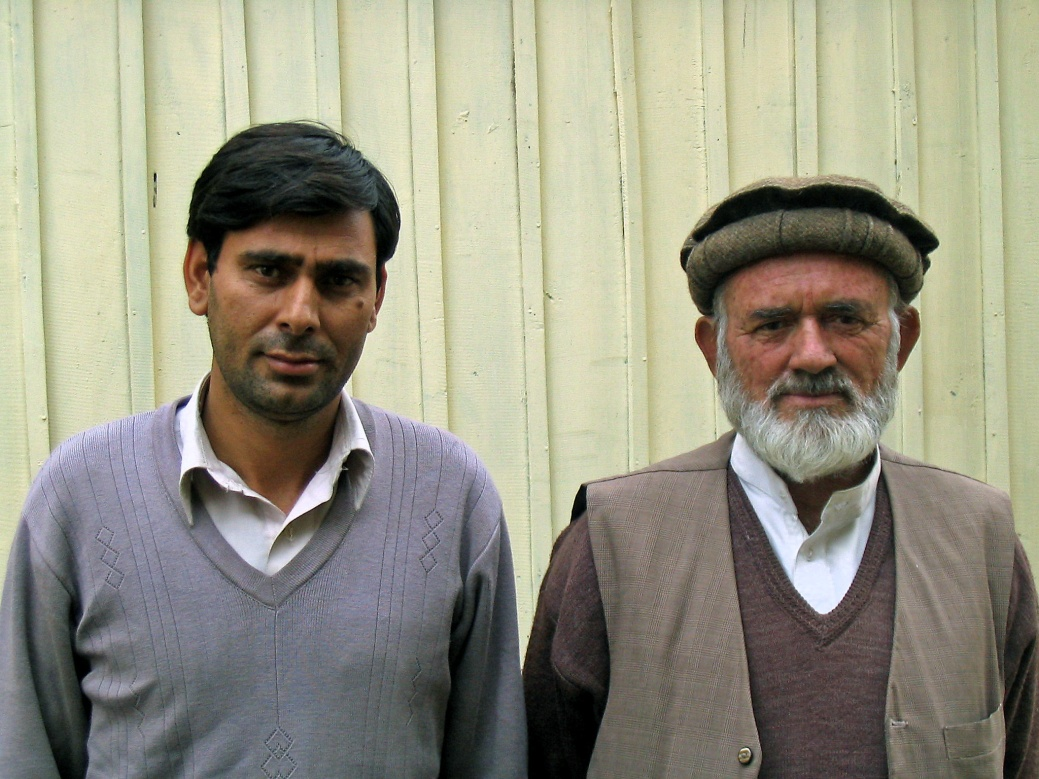
\includegraphics[width=\textwidth]{figures/ch1photo1.jpg}
\end{photofigure}

\textbf{Ikram ul"=Haq}, a~schoolteacher from Ashret, assisted me voluntarily in my research during
the period 1998--2000. He was introduced to transcription and basic recording methods and made
a~number of important interviews and text recordings, which he also transcribed and provided with
free translations.


\textbf{Sher Haider}, a~schoolteacher from Ashret and older brother of Naseem Haider, assisted me
voluntarily on different occasions, filling in questionnaires, providing natural examples and
explaining various aspects of his language. He participated in parts of the FLI training programme.


A few other people spent considerable time with me, contributing in important ways to my research,
understanding and ability to speak Palula: Saeed Ahmad, Kalkatak; Atah Ullah, Biori; and Sardar
Hayat, Ashret.


My material on phonology is primarily based on separate B. and A. word lists\footnote{This included
  lexemes (primarily nouns and verbs) recorded in differently inflected forms as well as recordings
  of words in isolation and in frames.} that I began compiling and recording with speakers in
1999. Those have been supplemented later with other lists and recordings.


The morphological and syntactic parts of my study are primarily based on text material, in all 60
texts from 36 speakers/writers, of different length and analysed with varying accuracy and
detail. Most of the texts are recorded and transcribed oral narratives, but also other textual
genres are represented. A few texts in the material were written and in some cases only later
recorded when read out. However, even those written texts represent an~oral rather than a~literary
style, as there is no literary tradition. A tentative orthography was introduced as late as 2004,
and the written texts were produced during an~experimental phase in its development. The textual
material was supplemented with elicitation of full paradigms, expressions and sentences,
questionnaires and notes of language use in the community.


For details on textual genres, types of data and individual speakers and writers or informants, the
list in \textit{References} at the end of this work should be consulted. The references given after
each example utterance throughout the work can be found in that list: Ex. A:SHY028 refers to
a~particular narrative (abbreviated SHY) in the Ashret variety (henceA:) written by Sher Haider, occurring as entry 28 in my interlinear text database.\footnote{A few texts are not entered as interlinear texts and therefore references to individual strings in them are not numbered.}


Although only marginally referred to and used, a~few smaller field studies carried out parallel with
my Palula research also need to be mentioned:


As already hinted at earlier, some \textbf{Sauji} data was collected in 2000, by Ajmal
Nuristani\footnote{Ajmal Nuristani's father is Nuristani and his mother's relatives come from Sau,
  but he is primarily a~Pashto speaker who grew up as a~refugee in Chitral.} and myself, in Timar
Camp in Lower Dir, where a~substantial number of people from Sau resided at the time. Later, Ajmal
Nuristani, on my request, recorded and transcribed a~few other texts and word lists, both in
Pakistan and in Sau (Afghanistan).


Also mentioned briefly above, a~survey trip to Kalkot in Dir Kohistan was carried out under Joan
Baart's (SIL) and my auspices by Naseem Haider and another FLI fellow, Muhammad Zaman Sager (from
Kalam, Swat), in 2006. Apart from obtaining sociolinguistic information, they recorded a~few
\textbf{Kalkoti} texts, a~word list with two different speakers, a~questionnaire focusing on verbs
and another focusing on pronouns.


As for \textbf{Dameli}, data was chiefly collected in the form of a~questionnaire (dealing with
pronouns and verb agreement) filled out in the summer of 2005 by Muhammad Hayat Jan of Aspar (Damel
Valley), who participated in the FLI training program. The data was subsequently discussed with and
commented upon by Emil Perder (Stockholm University).\footnote{Emil Perder began field work on
  Dameli in 2003, through FLI, mainly with the aforementioned Muhammad Hayat and Asmat Ullah, also
  from Aspar, as co"=researchers and informants.}


\begin{photofigure}[h!]
\caption{Cluster of houses in Mingal, Biori Valley (Dietmar Polster)}
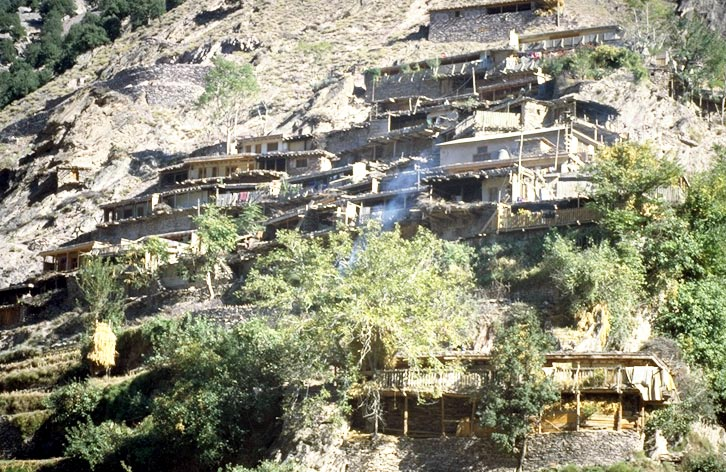
\includegraphics[width=\textwidth]{figures/ch1photo2.jpg}
\end{photofigure}


Also in 2005, I carried out some interviews (based on the questionnaire also used for Dameli) in Kalkatak with Muhammad Salaam and Faiz Muhammad, two \textbf{Gawarbati} speakers, both in their thirties and originally from Nari in Afghanistan and since the early 1980s settled in the refugee section of the village Kalkatak.\footnote{I am indebted to my friend and FLI colleague Fakhrud Din of Kalkatak for arranging these interviews.}


\section{Palula as a written language}
\label{sec:1-6b}

Until recently, Palula was unwritten and largely undocumented, a condition shared with most smaller (and even some larger) language communities in the region. Before the commencement of the current research, only a handful of local poets saw the need for writing Palula, making use of Urdu writing when composing poetry to be read aloud by themselves. There had been no systematic or collective attempts at creating a consistent and practical orthographic representation of Palula. The community is, after all, relatively small, with only a limited number of highly educated people, and uses a language entirely deprived of any outside recognition. Although there are primary schools throughout the Palula speaking area, only Urdu (and more recently English) is the recognized medium of instruction and formal literacy.


In 2003, representatives from all the major settlements came together and formed \textit{Anjuman-e-taraqqi-e-Palula}, a society for the promotion of Palula, with the purpose of facilitating the development of Palula as a vehicle for literary and educational efforts. At that time, an orthography proposal was put together by the authors of this work, with input from a few local scholars and teachers. It was endorsed by the society, which agreed that a Perso-Arabic script, conforming closely with the way it is applied to Urdu, should be used as a basis, with the addition of symbols representing a few consonant sounds not present in Urdu.\footnote{Words which are clearly identical with words in the Perso-Arabic stock are normally written in the traditional way, resulting in a fair degree of orthographic overrepresentation. The phoneme /s/ is, for example, represented by \PRL{<س>}
in most native Palula vocabulary, but could be written as \PRL{<س>}, \PRL{<ث>} or \PRL{<ص>} if occurring in a loanword, depending on the particular spelling in the donor language.} The alphabet adopted is presented in \tabref{tab:1-4b}. Starting with a group of Urdu-literate people, the basic spelling principles were further discussed and applied in a writers’ workshop in 2004. Following some fine-tuning of the orthography, the two first-ever Palula booklets were printed in 2006, one of them an alphabet book \citep{haider2006a}\footnote{A second edition was published in 2012 \citep{haider2012a}.} and the other a collection of short stories \citep{haider2006b}. In 2012, Forum for Language Initiatives and Anjuman-e-taraqqi-e-Palula published a collection of about 300 Palula proverbs and sayings, along with Urdu translations \citep{haider2012b}.


Through the Forum for Language Initiatives (at the time known as the Frontier Language Institute), the concept of multilingual education was introduced to the community in 2005. This eventually led to the establishment of a mother-tongue school in Ashret in 2008. More than 30 native Palula speakers, both men and women, took part in producing the curricula from scratch, representing a set of culturally relevant themes. In preparation for the first school year, a package was produced consisting of a pre-reader, a pre-writer, a primer, a collection of reading stories, a collection of listening stories, and a compilation of songs and rhymes, all in Palula. 


\begin{table}
\caption{The Palula alphabet with corresponding transcription (PCT)}
\begin{tabularx}{\textwidth}{ Q Q Q Q Q Q Q }
\lsptoprule
\PRL ج 
&\PRL ث 
&\PRL ٹ 
&\PRL ت 
&\PRL پ 
&\PRL ب 
&\PRL ا\\
\textit{ǰ} &
\textit{s} &
\textit{ṭ} &
\textit{t} &
\textit{p} &	
\textit{b} &	
\textit{a, aa}\\
\\
\PRL ڈ
&\PRL د 
&\PRL خ 
&\PRL ح 
&\PRL څ 
&\PRL ڇ 
&\PRL چ\\
\textit{ḍ} &
\textit{d} &
\textit{x} &
\textit{h} &
\textit{ts} &	
\textit{c̣} &	
\textit{č}\\
\\
\PRL س 
&\PRL ڙ 
&\PRL ژ 
&\PRL ز 
&\PRL ڑ 
&\PRL ر 
&\PRL ذ\\
\textit{s} &
\textit{ẓ} &
\textit{ǰ} &
\textit{z} &
\textit{ṛ} &	
\textit{r} &	
\textit{z}\\
\\
\PRL ع 
&\PRL ظ 
&\PRL ط 
&\PRL ض 
&\PRL ص 
&\PRL ݜ 
&\PRL ش\\
\textit{-} &
\textit{z} &
\textit{t} &
\textit{z} &
\textit{s} &	
\textit{ṣ} &	
\textit{š}\\
\\
\PRL م 
&\PRL ل 
&\PRL گ 
&\PRL ک 
&\PRL ق 
&\PRL ف 
&\PRL غ\\
\textit{m} &
\textit{l} &
\textit{ɡ} &
\textit{k} &
\textit{q} &	
\textit{f} &	
\textit{ɣ}\\
\\
\PRL ے 
&\PRL ی 
&\PRL ھ 
&\PRL ہ 
&\PRL و 
&\PRL ݨ 
&\PRL ن\\
\textit{ee} &
\textit{y, ii} &
\textit{h} &
\textit{h} &
\textit{w, oo} &	
\textit{ṇ} &	
\textit{n}\\\lspbottomrule
\end{tabularx}
\label{tab:1-4b}
\end{table}


% Table X: The Palula alphabet with corresponding transcription
% ج	ث	ٹ	ت	پ	ب	ا
% ǰ	s	ṭ	t	p	b	a, aa
% ڈ	د	خ	ح	څ	ڇ	چ
% ḍ	d	x	h	ts	c̣	č
% س	ڙ	ژ	ز	ڑ	ر	ذ
% s	ẓ	ǰ	z	ṛ	r	z
% ع	ظ	ط	ض	ص	ڜ	ش
% -	z	t	z	s	ṣ	š
% م	ل	گ	ک	ق	ف	غ
% m	l	ɡ	k	q	f	ɣ
% ے 	ی	ھ	ہ	و	ڻ	ن
% ee	y, ii	h	h	w, oo	ṇ	n


The most visible modifications made to the existing Urdu alphabet in order to write Palula have to do with symbols representing a number of retroflex sounds:\PRL{<ڇ>}  for \textit{c̣}, \PRL{<ڙ>} for \textit{ẓ}, \PRL{<ݜ>} for \textit{ṣ}, and \PRL{<ݨ>} for \textit{ṇ}. To write \textit{ts}, the symbol \PRL{<څ>} has been borrowed from the Pashto alphabet. Aspiration as well as \textit{h} occurring in clusters with voiced consonants (see \tabref{1-4bb}) are represented by \PRL{<ھ>}.


\begin{table}
\caption{Examples of Palula representation of ``aspiration''}
\begin{tabularx}{\textwidth}{ Q Q Q Q Q Q }
\lsptoprule
\PRL پھ 
&\PRL تھ 
&\PRL چھ 
&\PRL دھ 
&\PRL مھ 
&\PRL بھر\\
\textit{ph} &
\textit{th} &
\textit{čh} &
\textit{dh} &
\textit{mh} &
\textit{bhr}\\\lspbottomrule
\end{tabularx}
\label{tab:1-4bb}
\end{table}


Another modification relates to the representation of the ten vowels. Because of the many crucial contrasts between long and short vowels, particularly in word-final position, the developers of the Palula orthography introduced a language-particular use of a diacritic \PRL{<ۡ>} to mark a short vowel, as displayed in \tabref{tab:1-4c}. Mainly due to challenges in the area of font development, Palula materials are exclusively produced in naskh style, not in nasta’liq.


\begin{table}
\caption{Palula vowel representation}
\begin{tabularx}{\textwidth}{ Q Q Q Q Q }
\lsptoprule
\PRL اُو 
&\PRL او 
&\PRL ای 
&\PRL اے 
&\PRL آ\\
\textit{uu} &
\textit{oo} &
\textit{ii} &
\textit{ee} &
\textit{aa}\\
\PRL اُ 
&\PRL اوۡ 
&\PRL اِ 
&\PRL اےۡ 
&\PRL ا\\
\textit{u} &
\textit{o} &
\textit{i} &
\textit{e} &
\textit{a}\\\lspbottomrule
\end{tabularx}
\label{tab:1-4c}
\end{table}


% Table Y: Palula vowel representation
% اُو	او	ای	اے	آ
% uu	oo	ii	ee	aa
% اُ	اوۡ	اِ	اےۡ	ا
% u	o	i	e	a


\section{Remarks on the transcription}
\label{sec:1-7}

The trancription system used for Palula in the main bulk of this work (always occurring with
italics, ex. \textit{paaluulaá}) largely corresponds with that in general use in South Asian
linguistics and by most indologists (what \citeauthor{masica1991} refers to as ``Standard
Orientalist'', \citeyear[xv]{masica1991}, and some others refer to as an ``indological'' system,
\citealt[9]{radloff1999}).


Since this is also the basic system (with very slight variations) used by other contemporary
scholars of Shina varieties
(\citealt{buddruss1987,buddruss1993,buddruss1996,schmidtkohistani2001,schmidtkohistani2008,schmidt2000,schmidt2001,schmidt2002,schmidt2003,schmidt2004,radloff1992,radloff1999};
{Radloff w. Shakil \citeyear{radloffshakil1998}\footnote{Also the transcriptions in
    \citet{hook1990a,hook1996} and \citet{hookzia1987} agree to a~large extent with the principles
    applied by the other scholars.}, including the conventions for representing accent (for details,
  see \sectref{subsec:3-4-3}), I have seen no reason to abandon it in favour of any other standard, such as
  a~consistent use of IPA symbols, since any such decision would make inter"=variety comparisons more
  troublesome and less straight"=forward. This broad transcription, taking only phonological contrasts
  into account, I will refer to as \textit{Palula common transcription}.


However, to make the work accessible to the general typologist or readers not familiar with this
particular system, IPA transcription (following International Phonetic Association, 1999) has been
used (parallel with the Palula common transcription within parentheses) for phonemic and phonetic
transcription in Sections \sectref{sec:3-1}--\sectref{sec:3-4} of my Phonology chapter, the former consistently surrounded
by forward slashes, ex. /paːluːlǎː/, and the latter by square brackets, ex. [paːɫuːɫǎː]. The
symbols in my transcription deviating from IPA are presented in \tabref{tab:1-5}.


When citing other sources or scholars on individual IA languages, I have in most cases kept the
transcription used by them, without any attempts at making them conform to the particular
conventions used for Palula examples.


\begin{table}[ht]
\caption{Symbols used in Palula common transcription (PCT) deviating from IPA notation}
\begin{tabularx}{.8\textwidth}{ l l | Q }
\lsptoprule
PCT &
IPA &
Comment\\\hline
\textit{ṭ} &
ʈ &
\\
\textit{ḍ} &
ɖ &
\\
\textit{c̣} &
ʈʂ &
\\
\textit{č} &
ʨ &
\\
\textit{ṣ} &
ʂ &
\\
\textit{š} &
ɕ &
\\
\textit{ẓ} &
ʐ &
\\
\textit{ǰ} &
ʑ &\\


\textit{ṇ} &
ɳ &
\\
\textit{ṛ} &
ɽ &
\\
\textit{y} &
j &
\\
\textit{h} &
ʰ &
Aspiration (h following C in PCT)
\\
\textit{aa} &
aː &
Double vowel corr. to IPA length"=indicating /ː/
\\
\textit{áa} &
âː &
First"=mora accent
\\
\textit{aá} &
ǎː &
Second"=mora accent
\\
\textit{a}$\sim$ &
ã &
Nasalisation\\\lspbottomrule
\end{tabularx}
\label{tab:1-5}
\end{table}

I should hasten to add that the Palula common transcription is not to be considered a~practical
orthography. For that purpose the Arabic"=based script described in \sectref{sec:1-6b} is used and promoted in the community.

%% OLD
%% \begin{table}[ht]
%% \label{bkm:Ref193267319}
%% \caption{Symbols used in Palula common transcription (PCT) deviating from IPA notation}
%% \begin{tabularx}{\textwidth}{ l l | l l Q }
%% \lsptoprule
%% PCT &
%% IPA &
%% PCT &
%% IPA &
%% Comment\\\hline
%% \textit{ṭ} &
%% ʈ &
%% \textit{ṇ} &
%% ɳ &
%% \\
%% \textit{ḍ} &
%% ɖ &
%% \textit{ṛ} &
%% ɽ &
%% \\
%% \textit{c̣} &
%% ʈʂ &
%% \textit{y} &
%% j &
%% \\
%% \textit{č} &
%% ʨ &
%% \textit{h} &
%% ʰ &
%% Aspiration (h following C in PCT)\\
%% \textit{ṣ} &
%% ʂ &
%% \textit{aa} &
%% aː &
%% Double vowel corr. to IPA length"=indicating /ː/\\
%% \textit{š} &
%% ɕ &
%% \textit{áa} &
%% âː &
%% First"=mora accent\\
%% \textit{ẓ} &
%% ʐ &
%% \textit{aá} &
%% ǎː &
%% Second"=mora accent\\
%% \textit{ǰ} &
%% ʑ &
%% \textit{ã} &
%% ã &
%% Nasalisation\\\lspbottomrule
%% \end{tabularx}
%% \label{tab:1-5}
%% \end{table}
\chapter{Typological overview}
\label{chap:2}

This chapter is a~brief overview covering the most central features of Palula. For more in"=depth coverage of each topic, and for information on those not explicitly covered here, the later chapters will need to be consulted.


\section{Phonology}
\label{sec:2-1}


With its 32--37 members, the Palula consonant inventory (\tabref{tab:2-cons}) is moderately large to large \citep{maddieson_consonant_2013}. There are five basic places of articulation (labial, dental, retroflex, palatal and velar), with a~voicing contrast in the plosive and fricative sets, and an~aspiration contrast in the plosive and affricate sets. 


\begin{table}
\caption{Palula consonants}
\begin{tabularx}{\textwidth}{ Q Q Q Q Q Q Q }
\lsptoprule
p &
t &
ʈ &
&
k &
(q) &
\\
pʰ &
tʰ &
ʈʰ &
&
kʰ &
&
\\
b &
d &
ɖ &
&
ɡ &
&
\\
&
ʦ &
ʈʂ &
ʨ &
&
&
\\
&
(ʦʰ) &
(ʈʂʰ) &
ʨʰ &
&
&
\\
(f) &
s &
ʂ &
ɕ &
x &
&
h\\
&
z &
(ʐ) &
ʑ &
ɣ &
&
\\
m &
n &
ɳ &
&
&
&
\\
&
r &
ɽ &
&
&
&
\\
&
l &
&
&
&
&
\\
w &
&
&
j &
&
&
\\\lspbottomrule
\end{tabularx}
\label{tab:2-cons}
\end{table}


Palula has ten phonemic vowels, comprising five basic qualities, each having a~long and a~short counterpart. This inventory (\tabref{tab:2-voc}) forms a~symmetrical and typologically common system. Vowel nasalisation is a~marginal, possibly emerging, feature in the language, but not so far fully contrastive. 


\begin{table}
\caption{Palula vowels}
\begin{tabularx}{\textwidth}{ Q Q Q Q Q Q Q Q Q Q }
\lsptoprule
iː &
i &
&
&
&
&
&
&
uː &
u\\
&
&
eː &
e &
&
&
oː &
o &
&
\\
&
&
&
&
aː &
a &
&
&
&
\\\lspbottomrule
\end{tabularx}
\label{tab:2-voc}
\end{table}


The language has a~complex syllable structure \citep{maddieson_syllable_2013}, permitting three consonants in the onset position and two in the coda position (although a limited number of consonant combinations are permitted before or after the vowel nucleus, as shown in \tabref{tab:2-clusters}). There is a~tendency to drop the final consonant in word final clusters.


\begin{table}[ht]
\caption{Word boundary syllable clusters (vd = voiced; vl = voiceless)}
\begin{tabularx}{\textwidth}{ l l l l}
\lsptoprule
Types &
Combinations &
Examples \\\hline
CCC- &
vd plosive + /r/ + /h/&
/ɡrheːɳɖ/ &
`knot'\\
&
vd plosive/nasal + approximant + /h/&
/ˈdjhuːɽi/ &
`granddaughter'\\
CC- &
plosive/nasal + /r/ &
/kraːm/ &
`work'\\
&
consonant + approximant &
/ˈswaːnu/ &
`is sleeping'\\
&
vd consonant + /h/ &
/lhoːɳ/ &
`salt'\\
-CC &
nasal + consonant &
/ɡrhoːnk/ &
`worm'\\
&
vl fricative + vl plosive (/s + t/, /ʂ + ʈ/) &
/ɡhoːʂʈ/ &
`house'\\
&
/t/ + /r/ &
/putr/ &
`son'\\\lspbottomrule
\end{tabularx}
\label{tab:2-clusters}
\end{table}


Main stress falls on the final or the penultimate syllable of the lexical root. One of the vocalic moras of the stressed
syllable receives pitch accent, phonetically realised as: a) high level or high falling on a~short vowel
[\'{}], represented in this work as \textit{á} (in polysyllabic words, elsewhere no marking); b)
low rising on a~long vowel [\v{}], represented as \textit{aá}; or c) high falling on a~long vowel [\^{}],
represented as \textit{áa}. Pitch accent is contrastive, as illustrated in (\ref{ex:2-a}).


\begin{exe}
\extab
\label{ex:2-a}
\begin{tabularx}{116mm}{ l l l l l }
/seːtí/ (\textit{seetí})  &
vs &
/sêːti/ (\textit{séeti}) \\
`looked after' &
&
`thigh' \\
/děːdi/ (\textit{deédi})  &
vs &
/dêːdi/ (\textit{déedi})  \\
`burnt \textsc{f}' &
&
`grandmother' \\
/hár/ (\textit{har})  &
vs &
/hǎːr/ (\textit{haár})  &
vs &
/hâːr/ (\textit{háar}) \\
`every' &
&
`defeat' &
&
`take away!'\\
\end{tabularx}
\end{exe}


\section{Morphology}
\label{sec:2-2}

Palula morphology is suffixing, and formatives are almost exclusively concatenative \citep{bickel_fusion_2013}, with a~moderately high degreee of synthesis \citep{bickel_inflectional_2013}. 


Nouns are inflected for number (singular, plural) and case (nominative, oblique, genitive). In most of the declensional classes, nominative plural and oblique singular are cumulated into a~single formative \citep{bickel_exponence_2013}. The genitive (at least in the plural) can be analysed as suffixed to the oblique rather than to the nominative stem. The noun exemplified in \tabref{tab:2-nouns} is \textit{ṣinɡ} `horn'.

\begin{table}[ht]
\caption{Inflection of nouns}
\begin{tabularx}{\textwidth}{ Q Q Q }
\lsptoprule
&
Singular &
Plural
\\\hline
Nominative &
\textit{ṣinɡ} &
\textit{ṣínɡ-a}\\
Oblique &
\textit{ṣínɡ-a} &
\textit{ṣínɡ-am}\\ 
Genitive &
\textit{ṣínɡ-ii} &
\textit{ṣínɡ-am"=ii}
\\\lspbottomrule
\end{tabularx}
\label{tab:2-nouns}
\end{table}


There are three main functions of the oblique case of nouns: a) as the transitive subject in the perfective (i.e., as an ergative case marker); b) as the form to which postpositions are added; and c) as a~locative. A number of other case"=like functions (such as recipients) and more peripheral arguments appear as postpositional phrases.


Palula displays core"=case asymmetry \citep{iggesen_asymmetrical_2013}, within the category of nouns as well as for NPs in general (more on pronouns below). While most nouns (those belonging to the two major \textit{a}- and \textit{i}-declensions) make a~nominative"=oblique distinction, one declensional class (the \textit{m}-declension) in particular does not make this distinction at all, whereas some of the pronouns make an~even more fine"=tuned nominative"=accusative"=oblique distinction, as seen in \tabref{tab:2-case}.


\begin{table}[ht]
\caption{Core case distinctions}
\begin{tabularx}{\textwidth}{ l@{\hspace{25pt}} Q Q Q Q }
\lsptoprule
&
`man' &
`sister' &
`woman' &
\textsc{3sg}
\\\hline
Nominative &
\textit{míiš} &
\textit{bheéṇ} &
\textit{kúṛi} &
\textit{so} \\
Accusative &
\textit{míiš} &
\textit{bheéṇ} &
\textit{kúṛi} &
\textit{tas} \\
Oblique (=ergative) &
\textit{míiš-a} &
\textit{bheeṇ-í} &
\textit{kúṛi} &
\textit{tíi}
\\\lspbottomrule
\end{tabularx}
\label{tab:2-case}
\end{table}


Palula has a~fairly typical Indo"=European two"=gender system, which is primarily sex"=based \citep{corbett_sex-based_2013}. A noun is either masculine or feminine, a~property established through morphological agreement. The basis for gender assignment is semantic as well as formal \citep{corbett_systems_2013}.


The pronoun system proper (i.e., 1st and 2nd person) is interesting in that it makes more distinctions in the plural than in the singular (\tabref{tab:2-pron}), as there are dedicated ergative case forms only in the plural.\footnote{The forms \textit{ma} and \textit{tu} are glossed throughout this work as nominative and \textit{míi} and \textit{thíi} as genitive, regardless of their functions in the clause.}

\begin{table}[ht]
\caption{Pronominal case distinctions}
\begin{tabularx}{\textwidth}{ l Q Q Q Q }
\lsptoprule
&
Nominative &
Accusative &
Genitive &
Ergative
\\\hline
\textsc{1sg} &
\textit{ma} &
\textit{ma} &
\textit{míi} &
\textit{míi} \\
\textsc{2sg} &
\textit{tu} &
\textit{tu} &
\textit{thíi} &
\textit{thíi} \\
\textsc{1pl} &
\textit{be} &
\textit{asaám} &
\textit{asíi} &
\textit{asím} \\
\textsc{2pl} &
\textit{tus} &
\textit{tusaám} &
\textit{tusíi} &
\textit{tusím} 
\\\lspbottomrule
\end{tabularx}
\label{tab:2-pron}
\end{table}


The demonstratives, which are used as third"=person pronouns, essentially make the same case distinctions as the plural personal pronouns (although there are other uses of the oblique apart from its ergative function). Additionally, they display gender distinctions (in the nominative singular) as well as a~three"=way deictic contrast (\tabref{tab:2-dem}).


\begin{table}[ht]
\caption{Demonstrative distinctions}
\begin{tabularx}{\textwidth}{ l l l Q Q Q Q }
\lsptoprule
&
&
&
Nominative &
Accusative &
Genitive &
Oblique \\\hline
Proximal &
\textsc{sg} &
\textsc{m} &
\textit{nu} &
\textit{nis} &
\textit{nisíi} &
\textit{níi} \\
&
&
\textsc{f} &
\textit{ni} &
\textit{nis} &
\textit{nisíi} &
\textit{níi} \\
&
\textsc{pl} &
&
\textit{ni} &
\textit{ninaám} &
\textit{niníi} &
\textit{niním} \\
Distal &
\textsc{sg} &
\textsc{m} &
\textit{lo} &
\textit{las} &
\textit{lasíi} &
\textit{líi} \\
&
&
\textsc{f} &
\textit{le} &
\textit{las} &
\textit{lasíi} &
\textit{líi} \\
&
\textsc{pl} &
&
\textit{le} &
\textit{lanaám} &
\textit{laníi} &
\textit{laním} \\
Remote &
\textsc{sg} &
\textsc{m} &
\textit{so} &
\textit{tas} &
\textit{tasíi} &
\textit{tíi} \\
&
&
\textsc{f} &
\textit{se} &
\textit{tas} &
\textit{tasíi} &
\textit{tíi} \\
&
\textsc{pl} &
&
\textit{se} &
\textit{tanaám} &
\textit{taníi} &
\textit{taním} \\\lspbottomrule
\end{tabularx}
\label{tab:2-dem}
\end{table}


Adjectives are inflected for agreement in gender (masculine, feminine), number (singular, plural) and case (nominative, non"=nominative). The adjective in \tabref{tab:2-adj} is \textit{paṇáaru} `white'.


\begin{table}[ht]
\caption{Inflection of adjectives}
\begin{tabularx}{\textwidth}{ l l l Q }
\lsptoprule
&
Masculine singular &
Masculine plural &
Feminine\\\hline
Nominative &
\textit{paṇáaru} &
\textit{paṇáara} &
\textit{paṇéeri} \\
Non"=nominative &
\textit{paṇáara} &
\textit{paṇáara} &
\textit{paṇéeri} \\\lspbottomrule
\end{tabularx}
\label{tab:2-adj}
\end{table}


Finite verbs are inflected for tense("=aspect), mood (in a~limited sense) and agreement in a)
gender/number, \textit{or} b) person (the type of agreement expressed depending on tense-aspect, see \sectref{sec:2-3}
below). There are also some non"=finite forms. For the sake of a~more economical presentation that
takes verbs of different inflectional classes into account, all verbs are analysed as having
a~perfective and a~non"=perfective stem. The verb in \tabref{tab:2-verb} is \textit{til-} `walk'.


\begin{table}[ht]
\caption{Inflection of verbs}
\begin{tabularx}{\textwidth}{ l l Q Q }
\lsptoprule
&
&
Singular &
Plural \\\hline
\textbf{Non"=perfective stem} &
&
&
\\
Present &
\textsc{m} &
\textit{til-áan-u} &
\textit{til-áan-a} \\
&
\textsc{f} &
\textit{til-éen-i} &
\textit{til-éen"=im} \\
Future &
1 &
\textit{tíl-um} &
\textit{til-íia} \\
&
2 &
\textit{tíl-aṛ} &
\textit{tíl-at} \\
&
3 &
\textit{tíl-a} &
\textit{tíl-an} \\
Imperative &
&
\textit{tíl} &
\textit{tíl-ooi} \\
Infinitive &
&
\textit{til-áai} &
\\
Converb &
&
\textit{til-í} &
\\
Obligative &
&
\textit{til"=eeṇḍeéu} &
\\
Copredicative participle &
&
\textit{til-íim} &
\\
Verbal noun &
&
\textit{til"=ainií} &
\\
Agentive verbal noun &
\textsc{m} &
\textit{til-áaṭ-u} &
\textit{til-áaṭ-a} \\
&
\textsc{f} &
\textit{til-éeṭ-i} &
\textit{til-éeṭ-im} \\
\textbf{Perfective stem} &
&
&
\\
Perfective &
\textsc{m} &
\textit{tilíl-u} &
\textit{tilíl-a} \\
&
\textsc{f} &
\textit{tilíl-i} &
\textit{tilíl-im} \\\lspbottomrule
\end{tabularx}
\label{tab:2-verb}
\end{table}


\section{Syntax}
\label{sec:2-3}
Four of the most frequently occurring TMA"=categories (Future, Present, Simple Past (=perfective) and Imperative) make use of inflectional morphology only (as displayed in \tabref{tab:2-verb}).\footnote{Language"=specific, and functionally defined, verbal categories are capitalised to set them apart from grammatical terms applied cross"=linguistically. See Chapter \sectref{chap:9} for details.} Another three basic TMA"=categories (Past Imperfective, Perfect and Pluperfect) are expressed periphrastically, by adding auxiliaries to inflected verb forms (as shown in \tabref{tab:2-peri}).


\begin{table}[ht]
\caption{Periphrastically formed TMA"=categories}
\begin{tabularx}{\textwidth}{ l l Q Q }
\lsptoprule
TMA"=category &
Inflectional category &
Auxiliary &
Example \\\hline
Past Imperfective &
future &
\textsc{pst} &
\textit{tíl-um de} \\
Perfect &
perfective &
`be.\textsc{prs-agr}' &
\textit{tilíl-u hín-u} \\
Pluperfect &
perfective &
\textsc{pst} &
\textit{tilíl-u de} \\\lspbottomrule
\end{tabularx}
\label{tab:2-peri}
\end{table}


There is relatively little synchronically productive derivational morphology in the language, but a~productive process for deriving verbs from other categories from within the language as well as from entirely novel or non"=native elements is the use of verbalisers such as \textit{the-} `do' and \textit{bhe-} `become'. Some examples are shown in (\ref{ex:2-b}).


\begin{exe}
\extab
\label{ex:2-b}
\begin{tabularx}{116mm}{ l l l l l l l}
\textit{madád} &
`help' &
+ &
\textit{the-} &
{\textgreater} &
\textit{madád thíili} &
`helped'\\
\textit{tanɡ} &
`narrow' &
+ &
\textit{the-} &
{\textgreater} &
\textit{tanɡ thíilu} &
`troubled'\\
\textit{milaáu} &
`joined' &
+ &
\textit{bhe-} &
{\textgreater} &
\textit{milaáu bhílu} &
`met'\\
\textit{ašáq} &
`loving' &
+ &
\textit{bhe-} &
{\textgreater} &
\textit{ašáq bhílu} &
`fell in love with'\\
\end{tabularx}
\end{exe}


Word order in Palula is typically head"=final (\tabref{tab:2-worder}). This is seen in the word order in noun phrases (determiner--noun, adjective--noun, numeral--noun, genitive--noun), adjective phrases (adjunct--adjective) and in adpositional phrases (noun phrase--postposition). As far as entire clauses are concerned, the word order (or rather constituent order) is more flexible, but the most frequent and pragmatically unmarked order is intransitive subject--verb, transitive subject--verb, and direct object--verb.


\begin{table}[ht]
\caption{Word order features}
\begin{tabularx}{\textwidth}{ l l Q }
\lsptoprule
Order &
Example\\\hline
\textbf{Determiner}--noun &
\textit{\textbf{eesó} ḍhínɡar} &
`that wood' \\
\textbf{Adjective}--noun &
\textit{\textbf{paṇéeri} déeṛi} &
`white beard' \\
\textbf{Numeral}--noun &
\textit{\textbf{páanǰ} toobakí} &
`five rifles'\\
\textbf{Genitive}--noun &
\textit{\textbf{íṇc̣ii} rhaíi} &
`bear's footprints'\\
\textbf{Adjunct}--adjective &
\textit{\textbf{bíiḍi} dhríɡi} &
`very long'\\
\textbf{NP}--adposition &
\textit{\textbf{míi putrá} sanɡí} &
`with my son'\\
\textbf{S}--V &
\textit{\textbf{raaǰaá} múṛu} &
`The king died.'\\
\textbf{A}--V &
\textit{\textbf{tíi} áa ḍáaɡ mheerílu} &
`He killed a markhor.' \\
\textbf{O}--V &
\textit{tíi \textbf{áa ḍáaɡ} mheerílu} &
`He killed a markhor.' 
\\\lspbottomrule
\end{tabularx}
\label{tab:2-worder}
\end{table}


As far as alignment is concerned, Palula displays an~intricate split system. In the perfective categories (Simple Past, Perfect and Pluperfect), the pattern is essentially ergative, as seen in example (\ref{ex:2-1}), with a~non"=nominatively marked agent"=subject and verbal agreement with the feminine direct object. In the non"=perfective categories (Future, Present and Past Imperfective), in contrast, it is essentially accusative, which can be observed from the nominatively marked agent"=subject in (\ref{ex:2-2}), which is also the NP that the transitive verb agrees with in gender and number.

\begin{exe}
\ex
\label{ex:2-1}
\glll íṇc̣-a čhéeli khéel-i \\
bear[\textsc{msg}]-\textsc{obl} she.goat[\textsc{fsg}] eat.\textsc{pfv-}\textsc{f}\\
\textbf{A} \textbf{O} \textbf{V}\\
\glt `The bear ate the goat.' (A:PAS056)
\end{exe}


\begin{exe}
\ex
\label{ex:2-2}
\glll iṇc̣ áaṇc̣-a kha-áan-u\\
bear[\textsc{msg}] raspberry[\textsc{m}]-\textsc{pl} eat-\textsc{prs-msg} \\
\textbf{A} \textbf{O} \textbf{V}\\
\glt `The bear is eating raspberries.' (A:KAT145)
\end{exe} 


Agreement is part of all finite verb forms, but the particular agreement features realised are related to tense"=aspect. In Future and Past Imperfective, the verb agrees with its target in person (and number), as in (\ref{ex:2-3}), whereas in Present and the categories based on the perfective, the verb agrees in gender and number, as can be seen in (\ref{ex:2-4}).

\begin{exe}
\ex
\label{ex:2-3}
\glll so múṛee ǰand-óo de \\
\textsc{3msg.nom} dead.person.\textsc{pl} make.alive-\textsc{3sg} \textsc{pst} \\
\textbf{A} \textbf{O} \textbf{V} \\
\glt `He was resurrecting the dead.' (A:ABO034)
\end{exe}

\begin{exe}
\ex
\label{ex:2-4}
\glll táapaṛ-a túuri íṇc̣-a čhéeli ɡhašíl-i hín-i \\ 
hill-\textsc{obl} below bear[\textsc{msg}]-\textsc{obl} she.goat[\textsc{f}] catch.\textsc{pfv-f} be.\textsc{prs-f} \\
{} {} \textbf{A} \textbf{O} \textbf{V} \\
\glt `Below the hill, the bear has captured the goat.' (A:PAS054)
\end{exe}


Alignment in the realm of verbal alignment is summarized in \tabref{tab:2-verbagr}. 


\begin{table}[ht]
\caption{Alignment: Verbal agreement}
\begin{tabularx}{\textwidth}{ l l Q Q }
\lsptoprule
Aspect &
TMA"=category &
Agreement features &
Controller \\\hline
Non"=perfective &
Future, Past Imperfective &
Person/number &
S, A \\
&
Present &
Gender/number &
S, A \\
&
Imperative &
Number &
S, A \\
Perfective &
&
Gender/number &
S, O \\\lspbottomrule
\end{tabularx}
\label{tab:2-verbagr}
\end{table}


Several NP splits further complicate the picture. Apart from the singling out of the transitive subject (A) in the perfective (\textit{asím} in (\ref{ex:2-2a})), we also have pronominal forms particular to the direct object (O) (\textit{asaám} in (\ref{ex:2-2b})), both of them different from the form used as the subject (S) of an intransitive clause (\textit{be} in (\ref{ex:2-2c})).

\begin{exe}
\ex
\label{ex:2-2a}
\gll \textbf{asím} ǰinaazá khaṣeel-í wheelíl-u de \\
\textsc{1pl.erg} corpse drag-\textsc{cv} take.down.\textsc{pfv"=msg} \textsc{pst}  \\
\glt `We dragged the corpse down.' (A:GHA044)

\ex
\label{ex:2-2b}
\gll nu ba \textbf{asaám} mhaaranií the ukháat-u de \\
\textsc{3sg.prox.nom} \textsc{top} \textsc{1pl.acc} kill.\textsc{vn} to come.up.\textsc{pfv"=msg} \textsc{pst}  \\
\glt `He has come up here to kill us.' (A:HUA071)

\ex
\label{ex:2-2c}
\gll rhootašíi-a \textbf{be} ɡíia  \\
morning-\textsc{obl} \textsc{1pl.nom} go.\textsc{pfv.pl}  \\
\glt `In the morning we left.' (A:GHA006)
\end{exe}


Alignment in the realm of case marking is summarized in \tabref{tab:2-casealign}. This is a somewhat simplified overview in that some minor noun declensions (in which some case distinctions are upheld only in the plural) are not included.


\begin{table}[ht]
\caption{Alignment: Case marking}
\begin{tabularx}{\textwidth}{ l l Q }
\lsptoprule
NP"=type &
Aspect &
Case differentiation\\\hline
Nouns: \textit{a}- and \textit{i}-declensions &
Non"=perfective &
A=S=O \\
&
Perfective &
A≠S=O \\
Nouns: \textit{m}-declension &
&
A=S=O \\
Pronouns: \textsc{3sg, 1pl, 2pl, 3pl} &
Non"=perfective &
A=S≠O \\
&
Perfective &
A≠S≠O \\  
Pronouns: \textsc{1sg, 2sg} &
Non"=perfective &
A=S=O \\
&
Perfective &
A≠S=O
\\\lspbottomrule
\end{tabularx}
\label{tab:2-casealign}
\end{table}


Sentences lacking an~overt copula are allowed, and for predicate nominals in the Present tense, as the one shown in (\ref{ex:2-5}), they are typical.

\begin{exe}
\ex
\label{ex:2-5}
\gll míi báabu áak zamindaár míiš \\ 
\textsc{1sg.gen} father \textsc{idef} farmer man \\
\glt `My father is a~farmer.' (A:OUR002)
\end{exe}
Although it is possible to conjoin clauses with a~conjunctive suffix (also used for conjoining noun phrases), other strategies are preferred, such as juxtaposition for symmetrical clauses or the overwhelmingly favoured Converb construction, exemplified in (\ref{ex:2-6}), which is used for a~great variety of same"=subject clause combinations.

\begin{exe}
\ex
\label{ex:2-6}
\gll tíi ba [bhun wha-í ba] [so mhaás muṭ-í bhun wheel-í ba] [teeṇíi ɡhooṣṭ-á the ɡhin-í] ɡáu \\
\textsc{3sg.obl} \textsc{top} down come.down-\textsc{cv} \textsc{top} \textsc{def.msg.nom} meat tree-\textsc{gen} down take.down-\textsc{cv} \textsc{top} \textsc{refl} house-\textsc{obl} to take-\textsc{cv} go.\textsc{pfv.msg} \\
\glt `He came down [having come down], took down the meat from the tree [having taken down the meat from the tree], and brought it to his house.' (B:SHB762)
\end{exe}

In complex constructions, the unmarked order is a~complement clause followed by (or embedded in) the main clause, as in (\ref{ex:2-7}), and similarly an~adverbial clause followed by (or, again, embedded in) the main clause, as in (\ref{ex:2-8}). 

\begin{exe}
\ex
\label{ex:2-7}
\gll \textbf{neečíir} \textbf{theníi-e} díiš-e xalk-íim xwaaíš thíil-i \\
	hunt do.\textsc{vn"=gen} village\textsc{-gen} people\textsc{-pl.obl} desire do.\textsc{pfv-f} \\
\glt `People in the village wanted to go hunting.' (B:AVA200)
\end{exe}

\begin{exe}
\ex
\label{ex:2-8}
\gll \textbf{raaǰaá} \textbf{múṛ-u} \textbf{ta} putr-óom tasíi hukumát bulooṣṭéel-i \\
	king die.\textsc{pfv"=msg} \textsc{sub} son\textsc{-pl.obl} \textsc{3sg.gen} government snatch.\textsc{pfv-f} \\
\glt `When the king died, the sons seized the power.' (A:MAB003)
\end{exe}

However, a~post"=posed construction with the complementiser \textit{ki} is also commonly used (\ref{ex:2-9}), especially for utterance complements.

\begin{exe}
\ex
\label{ex:2-9}
\gll ɡhueeṇíi-am maníit-u ki \textbf{ni} \textbf{bíiḍ-a} \textbf{zinaawúr} \textbf{xálaka} \textbf{hín-a}\\
	Pashtun-\textsc{pl.obl} say.\textsc{pfv-msg} \textsc{comp} \textsc{3pl.prox.nom} much-\textsc{mpl} wild people be.\textsc{prs"=mpl} \\
\glt `The Pashtuns said, ``These are very wild people.''' (A:CHA008)
\end{exe}

Polar interrogatives are formed with a~clitical sentence"=final question particle \textit{ee} (B \textit{aa}), as in (\ref{ex:2-10}), whereas an~indefinite"=interrogative pronoun (or other proform), such as \textit{kasée} (B) `whose' in (\ref{ex:2-11}), is used in content interrogatives. 

\begin{exe}
\ex
\label{ex:2-10}
\gll ux-á díi khooǰóol-u ki tu insaán\textbf{=ee}\\
	camel-\textsc{obl} from ask.\textsc{pfv"=msg} \textsc{comp} \textsc{2sg.nom} human.being=\textsc{q} \\
\glt `He asked the camel, ``Are you a~man?''' (A:KIN007)
\end{exe}


\begin{exe}
\ex
\label{ex:2-11}
\gll aní \textbf{kasée} ziaarat-í thaní \\
	\textsc{prox.3pl.nom} whose shrine-\textsc{pl} \textsc{quot} \\
\glt `Whose shrines are these?' (B:FOR026)
\end{exe}

Negation is formed with a~separate and invariable negative particle \textit{na}, preceding the predicate (\ref{ex:2-12}).

\begin{exe}
\ex
\label{ex:2-12}
\gll muṣṭúk-a xálak-a dhii-á díi \textbf{na} khooǰ-óon de \\
	of.past-\textsc{mpl} people-\textsc{pl} daughter-\textsc{obl} from \textsc{neg} ask-\textsc{3pl} \textsc{pst} \\
\glt `People in the old days were not asking their daughter [who she wanted to marry].' (A:MAR018)
\end{exe}
\chapter{Phonology}
\label{chap:3}

\section{Consonants}
\label{sec:3-1}

\subsection{Consonant inventory}
\label{subsec:3-1-0}

\begin{table}[ht]
\caption{Inventory of consonants (IPA). Marginal or doubtful phonemes within parentheses}
\begin{tabularx}{\textwidth}{ P{20mm} Q Q Q Q Q Q Q Q }
\lsptoprule
&
La\-bi\-al &
Den\-tal &
Retro\-flex &
Pa\-la\-tal &
Ve\-lar &
Post\-velar &
Glot\-tal \\\hline
Plo\-sive
&
p &
t &
ʈ &
&
k &
(q) &
\\
&
pʰ &
tʰ &
ʈʰ &
&
kʰ &
&
\\
&
b &
d &
ɖ &
&
ɡ &
&
\\
Affricate
&
&
ʦ &
ʈʂ &
ʨ &
&
&
\\
&
&
(ʦʰ) &
(ʈʂʰ) &
ʨʰ &
&
&
\\
Fricative
&
(f) &
s &
ʂ &
ɕ &
x &
&
h\\
&
&
z &
(ʐ) &
ʑ &
ɣ &
&
\\
Nasal
&
m &
n &
ɳ &
&
&
&
\\
Flap
&
&
r &
ɽ &
&
&
&
\\
Lateral approximant
&
&
l &
&
&
&
&
\\
Approximant
&
w &
&
&
j &
&
&
\\\lspbottomrule
\end{tabularx}
\label{tab:3-1}
\end{table}

The consonant inventory is rather symmetrical, with the dental and retroflex places of articulation displaying the most well"=developed system of manner contrasts. The ancient (OIA) contrast between the three sibilants /s ʂ ɕ/ is preserved \citep[375]{cardonaluraghi2009}, with the present voicing contrast probably not evolving until quite recently, partly through lenition of voiced affricates, partly through foreign loans. 

While the plosive and fricative sets show a~contrast in voicing except for in the (marginal) labial and glottal places of articulation, voiced counterparts are missing in the small affricate set. Mirroring that is a~general allophonic variation (see below) between voiced fricative and affricate pronunciations. The voiced palatal fricative could equally well be treated as an~affricate, as that is the more common allophone (especially in the A dialect), but to provide more symmetry to the system, I have chosen to include it among the voiced fricatives,\footnote{As pointed out by \citet[34]{zoller2005}, this particular asymmetry within the affricate/fricative sets is a~feature shared by a~number of languages of northern Pakistan, due to a ``lenition process which is more advanced in case of the voiced phonemes than in case of the voiceless phonemes''.} while in the common transcription it is represented as \textit{ǰ}.


The post"=velar (or uvular) place of articulation is represented by a~voiceless post"=velar or uvular plosive /q/ alone. This marginal phoneme is only pronounced distinctly post"=velar by some educated speakers~-- and even then rather inconsistently~-- when occurring in loanwords of mainly Perso"=Arabic origin. In many speakers' pronunciation, however, it normally tends to approximate a~velar fricative pronunciation [x], thus not contrasting with the phoneme /x/. The fricatives /z, x, ɣ/ are rather frequent in present"=day Palula, and many of the words probably have a~long history in the language, although they to a~large extent are found in vocabulary borrowed from languages in the immediate region, and to a~much lesser extent are found in inherited vocabulary affected by phonological processes. A labio"=dental [f] is sometimes heard in more recent loans, primarily from Urdu and English, but with many speakers it alternates freely with or is entirely replaced by the native voiceless plosive /pʰ/, hence /f/ is considered a~marginal phoneme. 


The voiced retroflex fricative /ʐ/ is also a~marginal phoneme, but it is included for comparative reasons; an~even more rarely occurring voiced retroflex affricate sound [ɖʐ] is tentatively analysed as an~allophone of the same phoneme. 


There is insufficient proof to regard a~velar nasal [ŋ] as a~phoneme independent from /n/, as it only occurs before /k/ and /ɡ/, or as a~variant pronunciation of /nɡ/: [ŋɡ]$\sim$[ŋ]. 


Although initial findings identified several voiced aspirated consonants, later observations favoured a~cluster analysis, e.g., /b/ followed by /h/ rather than a~phoneme /bʰ/. However, it should be noted that voiceless aspirated sounds do share some characteristics with (frequently occurring) clusters of voiced consonants and /h/, as will be further discussed in \sectref{subsec:3-4-1}.

\subsection{Distribution and variation}
\label{subsec:3-1-1}

Examples of the distribution of consonants are shown in \tabref{tab:3-2}. 


The retroflex consonants are in some descriptions called ``retracted'' \citep[16]{schmidtkohistani2008} or ``cerebrals'' \citep{morgenstierne1941}; it has been questioned whether these consonants in HKIA languages are retroflex in the same sense or to the same extent as in the main NIA languages or in Dravidian languages. 


\begin{sidewaystable}[p!]
\caption{The distribution of consonants: word"=initial, medial, and final.{\protect\footnotemark}
  The occurrences within parentheses are matters of interpretation (see \sectref{subsec:3-2-3},
  \sectref{subsec:3-4-1})}
\begin{tabularx}{\textwidth}{ l@{\hspace{20pt}} l@{\hspace{20pt}} Q l@{\hspace{20pt}} Q Q Q Q }
\lsptoprule
/p/ &
&
/piːli/ &
`drank (\textsc{f})' &
/ɕopu/ &
`navel' &
/ʈip/ &
`drop'\\
/pʰ/ &
\textit{(ph)} &
/pʰoː/ &
`boy' &
/aɖapʰaːr/ &
`halfways' &
-- &
\\
/b/ &
&
/biːɖi/ &
`many (\textsc{f})' &
/ʑabal/ &
`iron bar' &
/ɖaːb/ &
`plain'\\
/f/ &
&
/fasil/ &
`crop' &
/xafa/ &
`upset' &
/muaːf/ &
`excuse'\\
/m/ &
&
/miːɕa/ &
`men' &
/hiːmaːl/ &
`glacier' &
/braːm/ &
`joint'\\
/w/ &
&
/wiːwaj/ &
`wife's brother' &
/heːwaːnd/ &
`winter' &
(/ɡhaːw/ &
`cow')\\
/r/ &
&
/reːti/ &
`nights' &
/beːriʂ/ &
`summer' &
/anɡoːr/ &
`fire'\\
/l/ &
&
/leːdi/ &
`found (\textsc{f})' &
/baliː/ &
`roof end' &
/ʨʰaːl/ &
`goat kid'\\
/t/ &
&
/teːti/ &
`hot (\textsc{f})' &
/pʰutu/ &
`fly' &
/baːt/ &
`word'\\
/tʰ/ &
\textit{(th)} &
/tʰuːɳi/ &
`pillar' &
/sutʰaːn/ &
`trousers' &
-- &
\\
/d/ &
&
/deːdi/ &
`father's mother' &
/leːdi/ &
`found (\textsc{f})' &
/ɕid/ &
`coldness'\\
/n/ &
&
/neːɽi/ &
`stream bed' &
/ʑaːnu/ &
`person' &
/soːn/ &
`pasture'\\
/s/ &
&
/seːti/ &
`looked after (\textsc{cv})' &
/buːsi/ &
`kiss' &
/deːs/ &
`day'\\
/z/ &
&
/zeːri/ &
`supplication' &
/baːzoːr/ &
`bazaar' &
/anɡreːz/ &
`Brit'\\
/ʦ/ &
\textit{(ts)} &
/ʦiːpi/ &
`squeezed (\textsc{cv})' &
/buʦu/ &
`stick' &
/uʦ/ &
`spring'\\
/ʦʰ/ &
\textit{(tsh)} &
-- &
&
/baʦʰaːr/ &
`calf' &
-- &
\\
/ɕ/ &
\textit{(š)} &
/ɕeːmi/ &
`spleen' &
/huːɕi/ &
`wind' &
/diːɕ/ &
`village'\\
/ʨ/ &
\textit{(č)} &
/ʨeːri/ &
`spouted jug' &
/kuʨuru/ &
`dog' &
/baːlbaʨ/ &
`child'\\
/ʨʰ/ &
\textit{(čh)} &
/ʨʰeːli/ &
`she"=goat' &
/piʨʰaː/ &
`swept  (\textsc{cv})' &
-- &
\\\lspbottomrule
\end{tabularx}
\end{sidewaystable}

\addtocounter{table}{-1}
\begin{sidewaystable}[p!]
\caption{The distribution of consonants: word"=initial, medial, and final. The
  occurrences within parentheses are matters of interpretation (see \sectref{subsec:3-2-3}, \sectref{subsec:3-4-1}). (continued)}
\begin{tabularx}{\textwidth}{ l@{\hspace{20pt}} l@{\hspace{20pt}} Q l@{\hspace{20pt}} Q Q Q Q }
\lsptoprule
/ʑ/ &
\textit{(ǰ)} &
/ʑeːli/ &
`bore (\textsc{f)}' &
/beːʑi/ &
`heifer' &
/raːʑ/ &
`rope'\\
/j/ &
\textit{(y)} &
/jiːɽi/ &
`sheep' &
/lhaːja/ &
`will find' &
(/babaːj/ &
`apple')\\
/ʈ/ &
\textit{(ṭ)} &
/ʈaːka/ &
`call!' &
/beːʈi/ &
`lamb' &
/baːʈ/ &
`stone'\\
/ʈʰ/ &
\textit{(ṭh)} &
/ʈʰonɡi/ &
`axe' &
/buʈʰeː/ &
`all' &
-- &
\\
/ɖ/ &
\textit{(ḍ)} &
/ɖaːka/ &
`robbery' &
/ɡeːɖi/ &
`big (\textsc{f)}' &
/haːɖ/ &
`bone'\\
/ɳ/ &
\textit{(ṇ)} &
-- &
&
/deːɳi/ &
`calf (of leg)' &
/bheːɳ/ &
`sister'\\
/ɽ/ &
\textit{(ṛ)} &
-- &
&
/deːɽi/ &
`beard' &
/kiroːɽ/ &
`chest'\\
/ʂ/ &
\textit{(ṣ)} &
/ʂeːti/ &
`disputed (\textsc{f)}' &
/kʰaʂiː/ &
`hoe' &
/baːʂ/ &
`rain'\\
/ʐ/ &
\textit{(ẓ)} &
/ʐami/ &
`sister's husband' &
/ʈʂaɳʐa/ &
`torch' &
/riːʐ/ &
`track'\\
/ʈʂ/ &
\textit{(c̣)} &
/ʈʂiːnki/ &
`twittered (\textsc{cv)}' &
/teːʈʂi/ &
`wood chisel' &
/drhaːʈʂ/ &
`grape'\\
/ʈʂʰ/ &
\textit{(c̣h)} &
/ʈʂʰiːr/ &
`milk' &
/aʈʂʰiː/ &
`eye' &
/buʈʂʰ/ &
`hunger'\\
/k/ &
&
/kati/ &
`how many?' &
/bakaːra/ &
`flock' &
/ɖoːk/ &
`back'\\
/kʰ/ &
\textit{(kh)} &
/kʰur/ &
`foot' &
/nikʰai/ &
`appeared (\textsc{cv)}'  &
-- &
\\
/ɡ/ &
&
/ɡaɖi/ &
`taken out (\textsc{cv)}' &
/siɡal/ &
`sand' &
/pʰaːɡ/ &
`fig'\\
/x/ &
&
/xati/ &
`letters' &
/maːxaːm/ &
`evening' &
/mux/ &
`face'\\
/q/ &
&
/qisa/ &
`story' &
/alaːqa/ &
`area' &
/aɕaq/ &
`love'\\
/ɣ/ &
&
/ɣeːri/ &
`caves' &
/kaːɣaːz/ &
`paper' &
/baːɣ/ &
`garden'\\
/h/ &
&
/hari/ &
`removed \textsc{(cv)}' &
(/kuhiː/ &
`well') &
-- &
\\\lspbottomrule
\end{tabularx}
\label{tab:3-2}
\end{sidewaystable}

\footnotetext{In Palula common transcription these would be: \textit{píili, šópu, ṭip, phoó, aḍaphaár, bíiḍi, ǰabál,
    ḍáab, fásil, xafá, muaáf, míiša, hiimaál, bráam, wíiwai,
    heewaánd, ɡhaáu, reetí, béeriṣ, anɡóor, léedi, balíi, čhaál,
    téeti, phútu, baát, thúuṇi, suthaán, déedi, léedi, šid, néeṛi, ǰáanu, sóon,
    seetí, búusi, deés, zeerí, baazóor, anɡreéz, tsiipí, bútsu, uts,
    batsaár, šéemi, húuši, díiš, čéeri, kučúru, baalbáč, čhéeli, pičhaá, ǰéeli,
    béeǰi, ráaǰ, yíiṛi, lháaya, babaái, ṭaaká, beeṭí, báaṭ, ṭhónɡi, buṭheé, 
    ḍaaká, ɡéeḍi, haáḍ, déeṇi, bheéṇ, déeṛi, kiroóṛ, ṣéeti,
    khaṣíi, báaṣ, ẓamí, ẓaṇẓá, ríiẓ, c̣iinkí, téec̣i, dhraác̣,
    c̣hiír, ac̣híi, buc̣h, katí, bakáara, ḍóok, khur, nikhaí, ɡaḍí, síɡal, phaáɡ, xatí, maaxaám, mux,
    qisá, alaaqá, ašáq, ɣeerí, kaaɣaáz, baáɣ, harí, kuhíi}.}



I am presently in no position to determine the exact nature of retroflexion in Palula, but I prefer, nevertheless, to retain the term, as the most prominent feature in the pronunciation of these consonants is the articulation with the tip of the tongue against a~place at the rear end of the alveolar ridge and usually with the tongue slightly curled back. The dental consonants on the other hand are indeed dental, often articulated against the lower as well as the upper teeth. Generally the area of contact between the tongue and the place of articulation is larger than in the case of the retroflex consonants.


The palatal consonants can also be described as alveolo"=palatal, with the blade of the tongue against the area covering the rear part of the alveolar and the front part of the palate, and with the tip of the tongue behind the lower teeth. 

\subsubsection*{Plosives}
The set of plosives includes: /p/: [p], /pʰ/: [pʰ]$\sim$[f], /b/: [b], /t/: [t̪], /tʰ/: [tʰ], /d/: [d̪], /ʈ/: [ʈ]$\sim$[ṯ], /ʈʰ/: [ʈʰ], /ɖ/: [ɖ]$\sim$[ḏ], /k/: [k], /kʰ/: [kʰ], /ɡ/: [ɡ], (/q/: [q]$\sim$[x]).

With respect to frequency, the voiceless plosives can be considered the unmarked subset, occurring almost twice as often as their voiced counterparts. The voiced plosives do not commonly occur word"=finally, and when they do they tend to be devoiced, as in /ɕid/ \textit{(šid)} `coldness': [ɕid̪̥]. Voiceless aspirated plosives occur in the majority of cases word"=initially, only seldom word"=medially, and never (as far as has been determined) in word"=final position. 


Intervocalically, the voiced plosives are often slightly fricativised, and frequently occur in clusters with /h/ (see \sectref{subsec:3-4-1}). Also, some of the voiceless aspirated plosives show lenition, for example /pʰ/ with an~alternating pronunciation [f]$\sim$[ɸ]$\sim$[pʰ], as in /pʰeːrimaː/ \textit{(pheerimaá)} `Ferima (\textsc{place name)}'. 


The phonemic status of [q] was already commented on above (see \sectref{subsec:3-1-0}).


\subsubsection*{Affricates}

The set of affricates includes: /ʦ/: [ts], /ʦʰ/: [tsʰ]$\sim$[s], /ʈʂ/: [ʈʂ], /ʈʂʰ/: [ʈʂʰ]$\sim$[ʂ], /ʨ/: [tɕ].


Affricates occur at three places of articulation, dental, retroflex and palatal, but with respect to frequency the dentals are quite limited as compared to the other two. The explanation of the missing voicing contrast is partly explainable (as already commented on above) by the overlap or neutralisation between the affricate and fricative sets. 


There is also a~less consistent neutralisation of the contrast between aspirated dental (\ref{ex:3-1}) and retroflex voiceless (\ref{ex:3-2}) affricates and their fricative counterparts (but as far as I have been able to observe, never between aspirated voiceless palatal affricates and fricatives), apparently limited to certain lexical items. 

\begin{exe}
\ex
\label{ex:3-1}
\gll atshareét \\
 /aʦʰareːt/: [aʦʰaɾěːt]$\sim$[asaɾěːt] \\
\glt `Ashret'

\ex
\label{ex:3-2}
\gll aaṣaáṛ \\
/aːʂaːṛ/: [aːʂǎːɽ]$\sim$[aːʈʂʰǎːɽ] \\
\glt `apricot'
\end{exe}

\subsubsection*{Fricatives}

The set of fricatives includes: (/f/: [f]$\sim$[pʰ]), /s/: [s], /z/: [z], /ʂ/: [ʂ]$\sim$[ʈʂʰ], /ʐ/: [ʐ]$\sim$[ɖʐ], /ɕ/: [ɕ], /ʑ/: [dʑ]$\sim$[ʑ], /x/: [x], /ɣ/: [ɣ], /h/: [ɦ]$\sim$[h].


As already pointed out in connection with the affricates, there is a~close link between the affricate set and the fricative set, with some overlaps and neutralisations taking place between them. The voiced palatal fricative is alternately realised as [ʑ] and [dʑ] (more often with an~affricate pronunciation in A) and the voiced retroflex as [ʐ] and [ɖʐ], whereas /z/ seems to occur consistently as [z] and never with an~affricate pronunciation.


The marginal phoneme /f/ is often realised as [pʰ], thus neutralised with /pʰ/, as in /faːjda/ \textit{(faaidá)} `benefit': [pʰaːjdá]$\sim$[faːjdá].


The voiced retroflex fricative is extremely rare, occurring only in a~few words. [ɖʐ] is most likely an~allophone of it, as in /ʐʰaɳʐiːr/ (ẓ\textit{haṇẓíir)} `chain': [ɖʐʰaɳɖʐ îːɾ]. 


There is a~strong affinity between /h/ and historical aspiration (\sectref{subsec:3-4-1}), especially when occurring in clusters of voiced consonants and /h/, in which case it is mostly realized as [ɦ]. Historical occurrences of word medial /h/ through movement to syllable onsets have most likely been reinterpreted as voiced aspiration. In the present language, a single /h/ only rarely occurs intervocalically, and even then often with an~interpretational ambivalence: \textit{(rhayíi)} `footprints': /rhajiː/ or /rahiː/.


\subsubsection*{Nasals}

The set of nasals includes: /m/: [m], /n/: [n̪]$\sim${}[ɲ]$\sim$[ŋ], /ɳ/: [ɳ].


Phonetically there are at least five places of articulation attested for nasals: labial, dental, retroflex, palatal and velar. The palatal nasal, however, is analysed as deriving from a~sequence of /n/ + a~palatal consonant, as it never occurs in any other environment. The same analysis may be applied to the velar nasal, where the sequence /n/ + a~velar stop usually is the likely source.


The case is a~little more complicated with the retroflex nasal, /ɳ/. Although it is clear in some cases that retroflexion is the result of assimilation with an~adjacent retroflex consonant, this cannot always be concluded. Whereas a~retroflex nasal normally does not occur word initially (although the word /ɳiɳeː/ \textit{(ṇiṇeé)} `popcorn' can be cited as an~isolated counterexample), it contrasts intervocalically with dental /n/, compare /deːni/ and /deːɳi/ in (\ref{ex:3-3}), and word"=finally, /kan/ and /kaɳ/ in (\ref{ex:3-4}). 

\begin{exe}
\ex
\label{ex:3-3}
\gll déeni -- déeṇi \\
/deːni/ -- /deːɳi/ \\
\glt `is giving'~-- `calf (of the leg)' 

\ex
\label{ex:3-4}
\gll kan -- kaṇ \\
/kan/ -- /kaɳ/ \\
\glt `shoulder'~-- `ear' (B)
\end{exe}

The labial and the dental nasals are very frequent in the language, as these two segments are part of some of the most productive inflectional forms in the language.

\subsubsection*{Flaps}

The set of flaps includes: /r/: [ɾ], /ɽ/: [ɽ].


While /r/ commonly occurs word"=initially, intervocalically, and word"=finally, the occurrence of /ɽ/
is more restricted. In B it does not occur word"=initially at all, whereas in A it occurs in free
variation with /l/ in weak forms of a~series of demonstratives (\ref{ex:3-5}), for example \textit{(lo)} or
\textit{(ṛo)} `he, that', related to strong forms of the same series with an~intervocalic
/ɽ/, \textit{(eeṛó)} `he, that', but otherwise not.

\begin{exe}
\ex
\label{ex:3-5}
\gll lo$\sim${}ṛo \\
/lo/$\sim${}/ɽo/ \\
\glt `he, that' 
\end{exe}

\subsubsection*{Lateral approximant}

There is one lateral approximant: /l/: [l]($\sim$[ɫ] B).


Preceded by a~back vowel /a aː o oː u uː/, /l/ is velarised, but only markedly so in the B variety: compare non"=velarised \textit{khéeli} and velarised \textit{khúulu} in (\ref{ex:3-6}).

\begin{exe}
\ex
\label{ex:3-6}
\gll khéeli~--~khúulu \\
/kʰeːli/~[kʰêːli]~-- /kʰuːlu/~[kʰûːɫu] \\ 
\glt `ate \textsc{fsg}'~-- `ate \textsc{msg}'
\end{exe}

\subsubsection*{Approximants}

The set of approximants includes: /w/: [β̞]$\sim$[ʋ], /y/: [j].


In the speech of my main A consultant, the front"=most approximant /w/ is usually pronounced bilabially [β̞], but with many speakers this phoneme seems to alternate between a~bilabial and something close to a~labiodental [ʋ] pronunciation.


The two approximants are sometimes challenging to interpret, whether they should be regarded as consonants or vowels, and they are in various ways susceptible to articulatory fluctuation or variation, especially when occurring intervocalically, an~issue that will be further discussed in connection with vowels (see \sectref{subsec:3-2-3}).


\section{Vowels}
\label{sec:3-2}

\subsection{Vowel inventory}

For the vowels, there are five contrasting places of articulation, as can be seen in \tabref{tab:3-3}: a) close front, b) close back, c) open front, d) open back rounded, and e) open back unrounded. Together with phonemic length contrasts, there is a~ten"=vowel system. A convincing and consistent contrast (as the one shown by \citet[19]{radloff1999} for Gilgiti Shina) between oral and nasalised vowels has not been found. Instead, nasalisation seems to be a~marginal suprasegmental feature of a~limited number of lexemes. Apart from those, nasalisation is a~non"=contrastive phonetic property of vowels occurring adjacent to a~nasal consonant. 



\begin{table}[ht]
\caption{Inventory of vowels, with IPA symbols}
\begin{tabularx}{\textwidth}{ Q Q Q Q Q }
\lsptoprule
&
&
Front
&
Back unrounded &
Back rounded \\\hline
Close &
short &
i &
&
u\\
&
long &
iː &
&
uː\\
Open &
short &
e &
a &
o\\
&
long &
eː &
aː &
oː\\\lspbottomrule
\end{tabularx}
\label{tab:3-3}
\end{table}

\subsection{Distribution and variation}
\label{subsec:3-2-1}

\tabref{tab:3-4} exemplifies target articulations of the vowels, all of which take on more centralised qualities in natural and connected speech. Generally, the short vowels /i/, /a/, and /u/ tend to be pronounced as less peripheral than their long counterparts. The short /i/ is not necessarily more open than the long /iː/, but it has a~rather more central pronunciation; the short /u/, on the other hand, is both more open and slightly more central than the long /uː/; the short /a/ is also slightly less open and more fronted than the long /aː/. 


\footnotetext{In Palula common transcription, the words are: \textit{ɡir, ɡiír, ṭíki, tíiṇi, preṣ, keéṇ, ṭéka, teeká, šak, káaṇ, ṭáka, ṭaaká, sum, kúuṇ, thúki, thúuṇi, khoṇḍ, kóoṇ, tróki, ṭooká}.}


\begin{table}[ht]
\caption{Vowel contrasts exemplified (see \sectref{subsec:3-4-3} for details on pitch accent){\protect\footnotemark}}
\begin{tabularx}{\textwidth}{ l l l@{\hspace{40pt}} l l l Q }
 \lsptoprule
/i/ &
/ɡir/ &
`turn around!' &
/iː/ &
\textit{(ii)} &
/ɡǐːr/ &
`saw'\\
&
/ʈíki/ &
`bread' &
&
&
/tî:ɳi/ &
`sharp'\\
/e/ &
/preʂ/ &
`mother"=in"=law' &
/eː/ &
\textit{(ee)} &
/kěːɳ/ &
`cave'\\
&
/ʈéka/ &
`peaks' &
&
&
/ʈeːká/ &
`labour'\\
/a/ &
/ɕak/ &
`doubt' &
/aː/ &
\textit{(aa)} &
/kâːɳ/ &
`ear'\\
&
/ʈáka/ &
`insult' &
&
&
/ʈaaká/ &
`call!' \\
/u/ &
/sum/ &
`dry mud' &
/uː/ &
\textit{(uu)} &
/kûːɳ/ &
`corner'\\
&
/tʰúki/ &
`spittle' &
&
&
/tʰûːɳi/ &
`pillar'\\
/o/ &
/kʰoṇḍ/ &
`speak!' &
/oː/ &
\textit{(oo)} &
/kôːɳ/ &
`arrow'\\
&
/tróki/ &
`worn, thin' &
&
&
/ʈoːká/ &
`push!' \\\lspbottomrule
\end{tabularx}
\label{tab:3-4}
\end{table}


Phonetically, there is a~significant difference between short and long vowels. The duration of a~long vowel like /aː/ as compared to its short counterpart /a/ is not just slightly longer, but usually of at least twice the duration.


Environment as well as accent (see \sectref{subsec:3-4-3}) further influences the exact pronunciation of each of the ten vowels. Under certain conditions, some neutralisations take place (see \sectref{subsec:3-2-2}). 


As pointed out already by \citet[58]{morgenstierne1932}, the most important~-- if not all~-- phonological dialect differences between A and B concern the vowels rather than the consonants. 

\subsection{Vowel neutralisation}
\label{subsec:3-2-2}

While there is a~consistent contrast between all the five vowel qualities as well as a~contrast in length, when the vowels are accented (see Section \sectref{subsec:3-4-3} for details on accent), these contrasts are fewer and less convincing when the vowels are unaccented. The two main dialects also show some differences in this regard. 


Whereas B maintains a~word"=final /a/ vs. /e/ contrast~-- as is clearly evidenced in the morphological contrast between the general oblique inflection \textit{-a}, as in /ˈdiːɕa/ `in the village', and the genitive singular \textit{-e}, as in /ˈdiːɕe/ `of the village', of many masculine nouns~-- there is no evidence of contrast between these two unaccented short vowels in A (where the unaccented genitive ending instead is /iː/). In contrast, a~non"=variable masculine ending [u] in B, corresponds to two different (but grammatically identical) masculine endings [o] and [u] in A. Curiously, the realizations of these two variants are in complementary distribution, although there is no obvious phonological motivation behind it. When preceded by /aː/ (in the previous syllable), the allophone is [u], while it is [o] when preceded by any other vowel, as can be seen in (\ref{ex:3-7}).

\begin{exe}
\ex
\label{ex:3-7}
\gll paṇáaru~-- tóoru~-- bhíiru~-- bhúuru~--  léku \\
[paɳâːɾu]~-- [tôːɾo]~-- [bɦîːɾo]~-- [bɦûːɾo]~-- [léko] \\ 
\glt `white \textsc{msg}'~-- `star [\textsc{m}]'~-- `he-goat [\textsc{m}]'~-- `deaf \textsc{msg}'~-- `small \textsc{msg}'
\end{exe}

As a consequence of these observations, all instances of unaccented word"=final [u] and [o] are consistently transcribed as \textit{u} in the Palula common transcription, whether A or B, and only word"=final unaccented \textit{a} occurs in A examples, not \textit{e}.


\subsection{The status of diphthongs}
\label{subsec:3-2-3}

A complex issue still needing more careful study concerns the interpretation and representation of ambiguous vowel sequences. However, for the time being there is no strong evidence for stipulating any phonemic diphthongs with a~status comparable to that of the ten vowels already introduced.

The sequences of vowels in lexical stems all consist of at least one close vowel (also interpretable as an~approximant), such as [ai], [aːi], [ui], [oːi], [oi], [eːi], [ueː], [uaː], [iaː], [ioː], [aːu], [au]. Probably most, if not all, combinations of a~short close vowel and another long or short vowel are possible. Some examples are given in (\ref{ex:3-8}).


\begin{exe}
\extab
\label{ex:3-8}
\begin{tabularx}{\textwidth}{ l l l l }
&
[bɾɦaːdʑai] &
\textit{(bhraaǰái)} &
`sister"=in"=law'\\
&
[baba:i] &
\textit{(babaái)} &
`apple'\\
&
[dʑabui] &
\textit{(ǰabúi)} &
`velum'\\
&
[bɦoːi] &
\textit{(bhoói)} &
`daughter"=in"=law'\\
&
[lɦoilo] &
\textit{(lhóilu)} &
`red'\\
&
[jeːi] &
\textit{(yéei)} &
`mother'\\
&
[kakueːki] &
\textit{(kakuéeki)} &
`hen'\\
&
[suaːl] &
\textit{(suaál)} &
`question'\\
&
[taːpiaːl] &
\textit{(taapiáal)} &
`near'\\
&
[pʰioːɽ] &
\textit{(phióoṛ)} &
`side (of an~animal)' \\
&
[ɡɦa:u] &
\textit{(ɡhaáu)} &
`cow'\\
&
[maɳɖau] &
\textit{(maṇḍáu)} &
`veranda'\\
\end{tabularx}
\end{exe}


Taking a~number of factors into account, such as mother"=tongue speakers' counting (``knocking'') syllables, the apparent absence of sequences not including any of the two close vowels [i] and [u], and the evidence for approximants occurring word"=initially as well as intervocalically (and therefore if not being interpreted consonantally leaving a~gap word"=finally), would favour an~approximant interpretation, which would render the following phonemic output: /brhaːˈʑaj/, /baˈbaːj/, /ʑaˈbuj/, /bhoːj/, /ˈlhojlu/, /jeːj/, /kakˈweːki/, /ˈswaːl/, /taːˈpjaːɽ/, /pʰjoːɽ/, /ɡhaːw/, /maɳˈɖaw/.


However, in a~number of words with a~vowel + [i] sequence, the final [i] can be considered a~feminine gender suffix (in some cases derived by that suffix, at least diachronically, from a~masculine stem), and in the morphological behaviour of monomorphemic stems, such as those exemplified above, it is an~advantage to show that there is an~underlying vowel /i/ or /u/ (rather than a~consonant) involved. Therefore, I have chosen to represent them as \textit{bhraaǰái}, \textit{yéei}, etc., in Palula common transcription, to signal precisely the connection between a~stem and its derivations or inflected forms.\footnote{Although not attempted here, an~alternative analysis of [ái] would be to consider it an~allophone of first"=mora accented /ée/.} 


The latter representation makes even more sense for sequences in polymorphemic words, such as \textit{dhióomii} `of the daughters' from \textit{dhií} + \textit{-óom} (\textsc{obl.pl)} + \textit{-ii} (\textsc{gen)}, although the surface phonemic representation would be /djhoːmiː/, the latter taking de facto syllabification into account at the expense of morphemic transparency. This holds for inflected forms of verbs as well: A purely phonemic representation such as /swâːnu/ `is sleeping \textsc{msg}' obscures the fact that we have the verbal stem \textit{só-} `sleep' inflected for present tense with \textit{-áan}, and therefore a~Palula common transcription \textit{suáanu} has been chosen for it.


When, on the other hand, there is a~need to show that there indeed is a~syllable break between two successive vowels, whether the word is mono- or polymorphemic, an~approximant, \textit{y} or \textit{w}, is inserted: \textit{bhooyóomii} /bhoːˈjoːmiː/ `of the daughters"=in"=law', and \textit{bharíiwa} /bhaˈriːwa/ `husbands'.


\section{Phonotactics}
\label{sec:3-3}

\subsection{Syllable structure}
\label{subsec:3-3-1}


A typical syllable in Palula is an~open syllable consisting of a~consonant and a~vowel. This is the most common type when the syllable is unaccented. Long, as well as short vowels (\ref{ex:3-9}) could constitute the nucleus of such a~syllable: CV or CVV. There are monosyllabic words (/be/, /wiː/) which conform to this basic CV pattern, but most words are polysyllabic, consisting of two or more CV (or CVV) syllables (such as /ɡuː.li/ and /ku.ɳaː.koː.miː/).


\begin{exe}
\extab
\label{ex:3-9}
\begin{tabular}{ l l l }
/be/ &
\textit{(be)} &
`we'\\
/wiː/ &
\textit{(wíi)} &
`water'\\
/ɡuː.li/ &
\textit{(ɡúuli)} &
`bread'\\
/ku.ɳaː.koː.miː/ &
\textit{(kuṇaakóomii)} &
`of the children'\\
\end{tabular}
\end{exe}



The closed"=syllable pattern, CV(V)C, is also a~very common syllable, see examples in (\ref{ex:3-10}), and the most common one in accented syllables. This type occurs in monosyllabic as well as in polysyllabic words. Commonly, however, a~word is made up of a~combination of open and closed syllables. 


\begin{exe}
\extab
\label{ex:3-10} 
\begin{tabular}{ l l l }
/pil/ &
\textit{(pil)} &
`drink!' \\
/ɕiːn/ &
\textit{(\v{s}íin)} &
`bed'\\
/ʈiːn.ʨuk/ &
\textit{(ṭíinčuk)} &
`scorpion'\\
/lan.ɡuːm/ &
\textit{(lanɡúum)} &
`I will take across'\\
/ʈom.bu/ &
\textit{(ṭómbu)} &
`stem'\\
/piɳ.ɖuː.ru/ &
\textit{(piṇḍúuru)} &
`round'\\
/heː.wan.da/ &
\textit{(heewandá)} &
`winter (\textsc{obl)}'\\
\end{tabular}
\end{exe}


Even onsetless syllables, V(C) or VV(C), occur in Palula (\ref{ex:3-11}), though less frequently. That means that both the onset and the coda is optional, i.e., a~vowel nucleus can occur alone or at least word"=initially. Whether this is also possible word"=medially or word"=finally is an~interpretational issue, but in any case, there are no single phonological words consisting of only a~vowel nucleus.\footnote{An alternative analysis not attempted in this work would be to regard a~glottal stop as a~consonant phoneme preceding all vowels that are here considered word"=initial, thus doing away with onsetless syllables altogether.}


\begin{exe}
\extab
\label{ex:3-11}
\begin{tabular}{ l l l }
/u.ɽi/ &
\textit{(uṛí)} &
`pour!' \\
/ux/ &
\textit{(ux)} &
`camel'\\
/oː.ɖhoːl/\ \ &
\textit{(ooḍhóol)} &
`flood'\\
\end{tabular}
\end{exe}


The minimal word can therefore be defined as consisting of a~vowel nucleus plus either an~onset or a~coda consonant. There seems also to be further constraints on words belonging to the major open classes as opposed to words from closed classes when it comes to minimal words. Nouns, adjectives and verbs (except for imperative forms and a~few participle forms) must consist of at least a~short vowel plus a~coda, or an~onset plus a~long vowel. Pronouns, on the other hand, may very well consist of only a~short vowel with an~onset: /ma/ `I', /be/ `we', etc.


\subsection{Consonant clusters}
\label{subsec:3-3-2}


The preservation of a~number of clusters, especially some that occur word finally, sets Palula off as more conservative than most other Shina varieties. In addition, a~set of changes, at least partly related to, on the one hand, vowel metathesis and re-syllabification, and on the other hand, laryngeal metathesis and the subsequent reinterpretation of what was earlier voiced aspirates (see \sectref{subsec:3-4-1}), have produced a few new, primarily word"=initial, clusters.


There is a~maximum onset of three consonants in Palula words, as can be seen in (\ref{ex:3-12}). These are clusters of voiced consonants only, whose third member always is /h/ (phonetically realized as [ɦ]).  One type, whose middle member is /r/ preceded by a plosive, go back to old (or secondarily formed) voiced aspirates followed by /r/. The aspirates have been reinterpreted as plosive + /h/ clusters, and a subsequent realignment has taken place, whereby the more sonorant /h/ has changed to the position closest to the syllable nucleus: /brhoː/ `brother' < */bhraː/ < \textit{bhr\'{\={a}}tr̥-}. Another type, whose middle member is one of the two approximants /j/ or /w/ (if we go with the analysis presented above, \sectref{subsec:3-2-3}) preceded by a plosive or a nasal, have arisen through de"=syllabification of a short unaccented closed vowel, in some cases subsequent to vowel metathesis, such as is the case (in A) with /ɡwheːɳiː/ `Pashtun' (< /ɡhweːɳiː/ < /ɡhueːɳiː/ < /uɡheːɳiː/, the latter which is still the form heard in the conservative B dialect). That other clusters similar to the last-mentioned type seem to be in the process of evolving is evidenced by co-existing forms: /ukʰaːndu/$\sim$/kʰwaːndu/ \textit{(ukháandu)} `is coming/going up \textsc{msg}', perhaps pointing to a~preference for Cw and Cj clusters vis-à-vis word initial V-syllables. 


\begin{exe}
\extab
\label{ex:3-12}
\begin{tabular}{ l l l l }
/brh-/ &
/brhoː/ &
\textit{(bhróo)} &
`brother'\\
/drh-/ &
/drhuːk/ &
\textit{(dhrúuk)} &
`gorge, stream' \\
/ɡrh-/ &
/ɡrheːɳɖ/ &
\textit{(ɡhreéṇḍ)} &
`knot' \\
/njh-/ &
/ˈnjhaːɽa/ &
\textit{(nhiáaṛa)} &
`near'\\
/djh-/ &
/ˈdjhuːɽi/ &
\textit{(dhiúuṛi)} &
`granddaughter'\\
/ɡwh-/ &
/ɡwheːˈɳiː/ &
\textit{(ɡhueeṇíi)} &
`Pashtun'\\
/dwh-/ &
/ˈdwheːli/ &
\textit{(dhuéeli)} &
`washed (\textsc{f)}'\\
\end{tabular}
\end{exe}


Initial two"=consonant clusters, see (\ref{ex:3-13}), share many of the features already mentioned for three"=consonant onsets. The second member of such a~cluster is either /r/ (most of them of considerable age), an~approximant (with a recent history, derived along the same lines as was presented above for /ɡwheːɳiː/), or /h/ (which is either historical voiced aspiration reinterpreted as a cluster, or a new initial cluster arisen through laryngeal metathesis). Usually, but not exclusively, /r/ is preceded by a~plosive (in the majority of cases a voiceless one). Voiceless aspirated plosives in clusters with /r/ are rare indeed, the verb /pʰrajaːnu/ `send' is the only example found so far in the data with a following /r/. Approximant may be preceded by plosive, fricatives or nasals. Nearly any voiced consonant may precede /h/ in initial clusters (the only exceptions in the data being the "new" phoneme /ɣ/, and the distributionally limited consonants /ɳ/ and /ɽ/).


\begin{exe}
\extab
\label{ex:3-13}
\begin{tabular}{ l l l l }
/pr-/ &
/ˈpraːʨu/ &
\textit{(práaču)} &
`guest'\\
/pʰr-/ &
/pʰraˈjaːnu/ &
\textit{(phrayáanu)} &
`is sending (\textsc{msg)}'\\
/br-/ &
/braːm/ &
\textit{(bráam)} &
`joint'\\
/tr-/ &
/ˈtroki/ &
\textit{(tróki)} &
`thin, weak (\textsc{f)}'\\
/kr-/ &
/kraːm/ &
\textit{(kráam)} &
`work' \\
/mr-/ &
/ˈmrinɡa/ &
\textit{(mrínɡa)} &
`deer'\\
/nj-/ &
/njaːˈʈa/ &
\textit{(niaaṭá)} &
`shave!, shear!' \\
/pj-/ &
/pjaːˈla/ &
\textit{(piaalá)} &
`cup'\\
/pʰj-/ &
/pʰjoːɽ/ &
\textit{(phióoṛ)} &
`side (of animal)' \\
/sw-/ &
/ˈsweːni/ &
\textit{(suéeni) } &
`is sleeping (\textsc{f)}'\\
/dh-/ &
/dhut/ &
\textit{(dhut)} &
`mouth'\\
/ʑh-/ &
/ʑhaːʈ/ &
\textit{(ǰhaáṭ)} &
`goat's hair'\\
/lh-/ &
/lhoːɳ/ &
\textit{(lhoóṇ) } &
`salt'\\
/mh-/ &
/mhaːs/ &
\textit{(mhaás)} &
`meat'\\
/jh-/ &
/ˈjhuɳɖi/ &
\textit{(yhúṇḍi)} &
`stick'\\
\end{tabular}
\end{exe}


Two"=consonant clusters in coda position, see (\ref{ex:3-14}), seem to be subject to a~much higher degree of variability, although the position also seems to be slightly more permissive than the onset. The more frequently occurring type observed at word boundaries consists of nasal + plosive/affricate/fricative, the other types being more marginal in occurrence. 


\begin{exe}
\extab
\label{ex:3-14}
\begin{tabular}{ l l l l }
/-nd/ &
/daːnd/ &
\textit{(dáand)} &
`tooth'\\
/-ɳɖ/ &
/ɡrheːɳɖ/ &
\textit{(ɡhreéṇḍ)} &
`knot'\\
/-nk/ &
/ɡrhoːnk/ &
\textit{(ɡhroónk)} &
`worm'\\
/-nɡ/ &
/ɕoːnɡ/ &
\textit{(šóonɡ) } &
`branch'\\
/-nʑ/ &
/paːnʑ/ &
\textit{(páanǰ) } &
`five' \\
/-nɕ/ &
/bheːnɕ/ &
\textit{(bheénš) } &
`beam (of wood)' \\
/-ɳʈʂ/ &
/iɳʈʂ/ &
\textit{(iṇc̣) } &
`bear' \\
/-tr/ &
/suːtr/ &
\textit{(súutr)} &
`thread' \\
/-st/ &
/ɡrhaːst/ &
\textit{(ɡhraást)} &
`wolf' \\
/-ʂʈ/ &
/ɡhoːʂʈ/ &
\textit{(ɡhoóṣṭ) } &
`house'\\
\end{tabular}
\end{exe}


The final affricate or fricative is always articulated, even if sometimes only weakly, whereas the
nasal (homorganic with the affricate or fricative) is sometimes~-- more with some speakers than
others and depending on word emphasis~-- phonetically absent but leaves a~trace of nasalisation on
the preceding vowel. Even the nasal + plosive sequences are subject to much variability. With some
speakers and dialects, one of the phonemes in the sequence is altogether absent, sometimes the nasal
(then leaving the preceding vowel nasalised, for example in /naːnɡ/
(náanɡ) `finger or toe"=nail' B: [n̪\^{ã}ːɡ]), sometimes the stop (for example in /ɕaːnɡ/ (\v{s}áanɡ)
`branch' B: [ɕâːŋ]), whereas in the corresponding inflected forms the stop would never be
omitted: [n̪ûːŋɡa] (núunɡa), [ɕûːŋɡa]
(\v{s}úunɡa). This especially pertains to the /n +
d/ sequences in singular nouns, where it seems to be more rule than exception that the final stop is dropped, especially in B, whereas these are clearly articulated when occurring non"=finally in the inflected forms: /dan/ `tooth', but /daːnda/ `teeth'; /pan/ `path', but /paːnda/ `paths'.


In the final /tr/-cluster, the /r/ is present as a~segment in the speech of all my informants, but its articulation is not exactly identical to its non"=final allophones (as in the inflected forms of the same lexical items). There is a~strong tendency for it to be pronounced with very little energy, almost always being devoiced and sometimes also followed by an~optional very short schwa"=like sound: [putɾ̥(ə)] in /putr/ `son'. 


As for the realisation of the final /st/ and /ʂʈ/-clusters, there are differences between different speakers, and possibly between different dialects as well. My B informants tend to articulate both members of the cluster, even in final position, though the plosive is somewhat softened, whereas my A informants seem to prefer to omit the plosive altogether in final position, e.g [ɡɦ\v{o}ːʂ] `house', [n̪aːs] \textit{(náas)} `nose'. However, in all speech varieties both the fricative and the plosive are clearly present when occurring medially, i.e., in the corresponding inflected forms: [ɡɦoːʂʈá], [nastí].


A special case is the final cluster /ndr/ in /jaːndr/, see (\ref{ex:3-15}). This is the only three"=consonant cluster at a~word boundary discovered so far, but its exact phonetic realisation is not entirely easy to define in terms of segments. With some speakers, the /n/ is clearly articulated, whereas the /dr/ part is only faintly present, and in other pronunciations the final /r/ gets a~schwa"=like sound attached to it, in practice making /dr/ the onset of an~additional syllable. As with the above"=mentioned clusters occurring at the end of singular nouns, the same cluster stretching over a~syllable boundary in an~inflected form of the same noun is clearly and unambiguously articulated: /jaːn.dra/ `mills'.


\begin{exe}
\extab
\label{ex:3-15}
\begin{tabular}{ l l l l }
/-ndr/ &
/jaːndr/ &
\textit{(yáandr)} &
`mill'\\
\end{tabular}
\end{exe}


Clusters occurring in syllable onsets and syllable codas intervocalically, see (\ref{ex:3-16}), are subject to the same restrictions as the clusters at word boundaries described above, but a few of them, particularly those containing /h/, are extremely rare in that position. 


\begin{exe}
\extab
\label{ex:3-16}
\begin{tabular}{ l l l l }
/-drh-/ &
/beːdrhiː/ &
\textit{(beedhríi)} &
`it [the sky] will clear up'\\
/-br-/ &
/ˈubru/ &
\textit{(úbru)} &
`a kind of bird'\\
/-tr-/ &
/ˈbaːtru/ &
\textit{(báatru)} &
`irrigation lock'\\
/-kr-/ &
/ˈʨukru/ &
\textit{(čúkru)} &
`sour'\\
/-dh-/ &
/badhoːˈɽaːnu/ &
\textit{(badhooṛáanu)} &
`is butting its horns (\textsc{msg)}'\\
/-nj-/ &
/dunˈjaː/ &
\textit{(duniaá)} &
`dowry'\\
/-mb-/ &
/oːmˈbaːr/ &
\textit{(oombaár)} &
`canal inlet'\\
/-nʨ-/ &
/ˈʈiːnʨuk/ &
\textit{(ṭíinčuk)} &
`scorpion'\\
\end{tabular}
\end{exe}


Apart from those, a number of other consonant clusters not permitted at word"=boundaries are found word"=internally. However, in all of those cases the clusters are analyzable as occurring across a syllable boundary (and not seldom across a morpheme"=boundary as well). Only a few examples are shown in (\ref{ex:3-17}).


\begin{exe}
\extab
\label{ex:3-17}
\begin{tabular}{ l l l l }
/-m.br-/ &
/ʑham.ˈbreːɽi/ &
\textit{(ǰhambréeṛi)} &
`bride'\\
/-ɕ.tr-/ &
/poːɕ.ˈtra/ &
\textit{(pooštrá)} &
`fattened'\\

\end{tabular}
\end{exe}


\section{Suprasegmentals}
\label{sec:3-4}

\subsection{Aspiration and breathiness}
\label{subsec:3-4-1}

In the present description, seven consonants, all voiceless, with aspiration as a~secondary articulation have been postulated: /pʰ/, /tʰ/, /ʈʰ/, /kʰ/, /ʦʰ/, /ʈʂʰ/, and /ʨʰ/. The two affricates /ʦʰ/ and /ʈʂʰ/ are treated with a~higher degree of tentativeness, as their contrastiveness vis-à-vis their non-aspirated counterparts is far less convincing than is the case with the other five aspirated segments, and would deserve further, more detailed, investigation.\footnote{At least as far as /ʈʂ/ is concerned, it seems, it is almost by ``default'' more or less clearly aspirated. A similar hesitation has been expressed on the /ʈʂ/-/ʈʂʰ/ contrast in Khowar \citep[239]{endresenkristiansen1981}.} There are, however, certain characteristics (synchronic as well as diachronic) that the voiceless aspirated sounds share with clusters of voiced consonants and /h/ (as described in \ref{subsec:3-3-2}), suggesting an alternative (or perhaps complementary), unitary treatment of aspiration as a~feature of a~word (or more correctly the lexical stem), as is already reflected in the consistent use of \textit{h} in the Palula common transcription.\footnote{It is also possible that a~more careful analysis will result in all instances of /h/ (here considered a~consonant in its own right when occurring alone in syllable onset) being treated in the same way.} 


This feature, realized as [ʰ] with a~voiceless consonant and [ɦ] (or [ʱ]) with a~voiced consonant, occurs only once in a~word\footnote{\label{fnt:ftn32} The process of dissimilation of aspirates in two successive syllables is known as \textit{Grassman's Law} within Indo"=European historical linguistics (\citealt[19, 56]{szemerenyi1996}; \citealt[153--154, 162--163]{lehmann1992}) and has been applied to the development of OIA as well as Greek. A synchronic process or rule restricting the occurrence of aspirated sounds to one per word has also been stipulated for other NIA languages (see for example \citet[32]{losey2002} for Gojri, and \citet[34--35]{shackle1976} for Siraiki). This process, however, is not confined to Indo"=European languages (compare Tibeto"=Burman Manipuri \citep[13--14]{bhatningomba1997}).} (in a~majority of the cases word"=intially). Some minimal pairs in (\ref{ex:3-18}) illustrate the contrastiveness of this feature.


\begin{exe}
\extab
\label{ex:3-18}
\begin{tabularx}{116mm}{ l l l }
/ˈbhoːla/ \textit{(bhóola)} &
vs &
/ˈboːla/ \textit{(bóola)}\\
`were able to' &
&
`hair'\\
/kʰaˈreːɽi/ \textit{(kharéeṛi)} &
&
/kaˈreːɽi/ \textit{(karéeṛi)}\\
`bolt' &
&
`leopardess'\\
/ˈʨʰeːli/ \textit{(čhéeli)} &
&
/ˈʨeːli/ \textit{(čéeli)}\\
`she"=goat' &
&
`wide (\textsc{f})'\\
/whiː/ \textit{(whíi)} &
&
/wiː/ \textit{(wíi)}\\
`will come down (\textsc{3sg})' &
&
`water'\\
\end{tabularx}
\end{exe}


The vowel immediately following /h/ occurring in clusters with voiced consonants is normally phonetically realised with (at least partially) breathy voice: [bʱo̤ːla]. 


Most voiced consonants can occur in clusters with /h/, from plosives to approximants (as described in \ref{subsec:3-3-2}). This generous occurrence of aspiration (in the wider sense) is not a~feature of most other languages in the immediate region, possibly with the exception of Indus Kohistani, where OIA aspiration, like in Palula, has been preserved and where aspiration is concomitant with most of its consonants \citep[19--25]{hallberghallberg1999}. 


Whereas the phonetic realisation of the aspiration with the voiceless consonants is more or less equal to a~secondary pronunciation of the voiceless segment, the ``breathiness'' affecting the pronunciation of the following vowel is somewhat mobile within the syllable, and for some words even beyond the realm of that syllable. Especially in B, there is a~fluctuation in some words, as seen in (\ref{ex:3-20}) and (\ref{ex:3-21}), between a~realization as a single intervocalic /h/"=segment and the occurrence of /h/ as part of a word"=initial cluster, as described above, the intervocalic /h/ probably representing an~older pattern.\footnote{Possibly this is preserved to a~larger extent in the conservative variety spoken in Puri (mainly agreeing with Biori Palula), where the following nominative"=oblique alternation was recorded: /brhuː/ \textit{(bhruú)} `brother' vs. /brahu/ `brothers'. The unstable character of the phoneme /h/ and voiced aspiration in Kalasha is also commented on by \citet[50]{morchheegaard1997}.}

\begin{exe}
\extab
\label{ex:3-20}
/lhójlo/$\sim$/lohílo/ \\
\textit{(lhóilu)} \\
`red' (B)

\extab
\label{ex:3-21}
/bjhûːɽi/$\sim$/bihûːɽi/ \\
\textit{(bhiúuṛi)} \\
`Biori' (B)
\end{exe}

In A, too, there are words, as in example (\ref{ex:3-22}), for which the location of aspriation is alternating (between speakers and possibly even with one and the same speaker).

\begin{exe}
\extab
\label{ex:3-22}
/ɡhaɖeːró/$\sim$/ɡaɖheːró/ \\
\textit{(ɡhaḍeeró)} \\
`elder'
\end{exe}

The aspiration feature (whether synchronically a cluster with /h/ or a voiceless aspirated consonant) has multiple diachronic sources: One is the OIA aspiration, thus preserved in Palula to an~extent not evidenced in the major Shina varieties,\footnote{On the contrary, \citet[30]{schmidtkohistani2008} state that the voiced aspirates in modern Kohistani Shina have come into the language through borrowing, while they have been lost in OIA voiced aspirate cognates.} such as in /ɡhuːɽu/ \textit{(ɡhúuṛu)} `horse' {\textless} OIA \textit{ɡhōṭa} \citep[4516]{turner1966}. Another is the above"=mentioned intervocalic /h/ advanced to a~more word"=initial position. Finally, an~old point of aspiration can be advanced, such as in /ɡhoːʂʈ/ \textit{(ɡhoóṣṭ)} `house' {\textless} OIA \textit{ɡōṣṭhá} \citep[4336]{turner1966}. Other words may have followed other routes, possibly further reinforced by the rising pitch of a~second mora accent (see \sectref{subsec:3-4-3} below). In any case, not all occurrences of aspiration, even when concomitant with plosives, are justified or explained solely by etymology (as pointed out by \citealt[57]{morgenstierne1932}).


Further study is needed to determine to what extent aspiration is preserved in two aspirated words that are compounded. There is an~indication that the primary stressed part of the compound keeps its aspiration, while the other point of aspiration is entirely or partly deaspirated (compare with the comment in footnote \ref{fnt:ftn32} on \textit{Grassman's Law}): /dhut/ \textit{(dhut)} `mouth' + /ɡhaːnu/ \textit{(ɡháanu)} `large' {\textgreater} /dutaɡhaːnu/ \textit{(dutaɡháanu)} `talkative'.


The interaction between accent and aspiration is another topic for further research. As breathiness (or a voiced cluster with /h/) quite often precedes a~second"=mora accented long vowel, the feature may have influenced or reinforced the rising pitch of that accent. However, it should be pointed out that breathiness also occurs before unaccented, as in /ʑhamatroː/ \textit{(ǰhamatroó)} `son"=in"=law', as well as first"=mora accented vowels, as in /oːɖhoːl/ \textit{(ooḍhóol)} `flood'; hence the two suprasegmental features are, in essence, independent.\footnote{This contrasts with the situation in Gawri and Torwali (both languages belonging to the Kohistani group of HKIA languages), where aspiration is only contrastive with voiceless consonants, whereas breathiness is a~feature only optionally concomitant with low tone (\citealt[92]{baart1999b}; \citealt[36--37]{lunsford2001}). } 


\subsection{Nasalisation}
\label{subsec:3-4-2}


As mentioned earlier, obligatory nasalisation seems to be a~marginal suprasegmental feature associated with an~extremely limited number of lexemes, among which figure those in (\ref{ex:3-23}). It is unclear whether in all those lexemes there is a~historical loss of a~nasal segment. In any case, there are too few instances to postulate any individual nasalized vowel phonemes, or even less a whole set of nasalized vowels. Neither are there in the data any examples of a lexical distinction being made solely by contrasting an~oral vowel with a~corresponding nasalized vowel. 


\begin{exe}
\extab
\label{ex:3-23}
\begin{tabularx}{\textwidth}{ l l l }
/ʑh\~{i}ː/ &
\textit{(ǰhií$\sim$) } &
`louse'\\
/kũj/ &
\textit{(kúi$\sim$)} &
`valley'\\
/bãːˈjilu/ &
\textit{(baa$\sim$ílu)} &
`made of oak wood'\\
/hẽː/ &
\textit{(hée$\sim$)} &
`yes'\\
/õː/ &
\textit{(óo$\sim$)} &
`mouth'\\
/drhũːʂ/ &
\textit{(dhrúu$\sim$ṣ)} &
`Drosh (a place)'\\
\end{tabularx}
\end{exe}

\subsection{Pitch accent}
\label{subsec:3-4-3}

A phonological word in Palula may carry one, and only one, accent. Phonetically the accent is primarily realised as relatively higher pitch, accompanied to some extent by higher amplitude. Generally speaking, in a~single word, accent is associated with high pitch, and the corresponding lack of accent is associated with low (or default) pitch. 

The accent"=bearing unit is the vocalic mora, which means that accent can be associated with a~short vowel (as in (\ref{ex:3-24})), or with the first mora of a~long vowel (as in (\ref{ex:3-25})), or with the second mora of a~long vowel (as in (\ref{ex:3-26})).


\begin{exe}
\extab
\label{ex:3-24}
\begin{tabularx}{\textwidth}{ l l l }
\multicolumn{3}{l}{Accent on short vowel:}\\
/ʂíʂ/ &
\textit{(ṣiṣ)} &
`head'\\
/híɽu/ &
\textit{(híṛu)} &
`heart'\\
/kilí/ &
\textit{(kilí)} &
`key'\\
\end{tabularx}
\end{exe}

\begin{exe}
\extab
\label{ex:3-25}
\begin{tabularx}{\textwidth}{ l l l }
\multicolumn{3}{ l}{First"=mora accent on long vowel:}\\
/ɖôːk/ &
\textit{(ḍóok)} &
`back'\\
/pûːtri/ &
(\textit{púutri)} &
`granddaughter'\\
/aʈʂîː/ &
\textit{(ac̣híi)} &
`eye'\\
\end{tabularx}
\end{exe}


\begin{exe}
\extab
\label{ex:3-26}
\begin{tabularx}{\textwidth}{ l l l }
\multicolumn{3}{ l}{Second"=mora accent on long vowel:}\\
/bǎːt/ &
\textit{(baát)} &
`talk, word, issue'\\
/kuɳǎːk/ &
\textit{(kuṇaák)} &
`child'\\
/bǎːbu/ &
\textit{(baábu)} &
`father'\\
\end{tabularx}
\end{exe}

This means that the pitch accent\footnote{Pitch accent here is of the kind also observed in e.g., Lithuanian \citep[73--82]{szemerenyi1996}, a~mora accent which is ``free within limits''.} (henceforth only ``accent'') has one of the following phonetic manifestations:
\begin{enumerate}
\item[a)] high level or falling on a~short vowel [\'{}], represented in this work with an~acute accent mark: \textit{á} (only in polysyllabic words, elsewhere without marking), 
\item[b)] rising on a~long vowel [\v{}], represented with an~acute accent mark on the second vowel symbol: \textit{aá}, or 
\item[c)] falling on a~long vowel [\^{}], represented with an~acute accent mark on the first vowel symbol: \textit{áa}.
\end{enumerate}
A word, as referred to here, is either a~bare stem, such as /děːs/ \textit{(deés)} `day', /paːɽú/ \textit{(paaṛú)} `magician', or a~stem with one or more suffixes added to it, such as /deːs-ôːm-iː/ \textit{(dees-óom"=ii)} `of the days', /ʑhôːn-um/ \textit{(ǰhóon"=um)} `I will know'. Even though some combinations of syllables and accents are more common than others and there are restrictions on accent placement (see below), the location of the accent within a~given word is not entirely predictable. Therefore, accent in Palula must be defined as lexical. 


Difference in accent placement is in a~few cases, as in (\ref{ex:3-27}), the only phonemic contrast between two lexical items.


\begin{exe}
\extab
\label{ex:3-27}
\begin{tabularx}{116mm}{ l l l l l }
/ʨûːr/ \textit{(čúur)} &
`four' &
vs &
/ʨǔːr/ \textit{(čuúr)} &
`hot fire'\\
/káti/ \textit{(káti)} &
`saddle' &
&
/katí/ \textit{(katí)} &
`how many?'\\
/dêːdi/ \textit{(déedi)} &
`grandmother' &
&
/děːdi/ \textit{(deédi)} &
`burnt'\\
/dhûːra/ \textit{(dhúura)} &
`distant' &
&
/dhuːrá/ \textit{(dhuurá)} &
`separate'\\
\end{tabularx}
\end{exe}

Although this kind of minimal pair is not particularly common in the language, the system definitely allows them to occur.

\subsubsection*{The position of accent on stems}

Accent falls either on the final or the penultimate syllable in a~non"=verbal lexical stem, as seen
in (\ref{ex:3-28}) and (\ref{ex:3-29}); whereas in verbal stems, as in (\ref{ex:3-30}), the accent
is always on the final syllable. In terms of vocalic moras, only one of the three last moras, of any lexical stem in Palula, may be the locus of the pitch accent.


\begin{exe}
\extab
\label{ex:3-28}
\begin{tabularx}{\textwidth}{ l l l }
\multicolumn{3}{l}{Accent on noun stems:}\\
/tôːruɳ/ &
\textit{(tóoruṇ)} &
`forehead'\\
/paːlǎː/ &
\textit{(paalaá)} &
`leaf'\\
/kakarîː/ &
\textit{(kakaríi)} &
`skull'\\
/kuɳôːku/ &
\textit{(kuṇóoku)} &
`puppy'\\
/ɡhaɖeːró/ &
\textit{(ɡhaḍeeró)} &
`elder'\\
\end{tabularx}

\extab
\label{ex:3-29}
\begin{tabularx}{\textwidth}{ l l l }
\multicolumn{3}{ l }{Accent on some other non"=verbal stems:}\\
/típa/ &
\textit{(típa)} &
`now'\\
/pʰaré/ &
\textit{(pharé)} &
`along, toward'\\
/eːtríli/ &
\textit{(eetríli)} &
`the day before yesterday'\\
/taːqatwár/ &
\textit{(taaqatwár)} &
`powerful'\\
/ǒːra/ &
\textit{(oóra)} &
`over here'\\
\end{tabularx}

\extab
\label{ex:3-30}
\begin{tabularx}{\textwidth}{ l l l }
\multicolumn{3}{ l}{Accent on verb stems:}\\
/krín-/ &
\textit{(krín-)} &
`sell'\\
/piʨʰíl-/ &
\textit{(pičhíl-)} &
`slip'\\
/karoːɽé-/ &
\textit{(karooṛé-)} &
`dig, scratch'\\
/nûːʈ-/ &
\textit{(núuṭ-)} &
`return'\\
\end{tabularx}
\end{exe}

\subsubsection*{Accent properties of suffixes}

There are two types of suffixes: those that carry their own accent, which will be referred to as
accent"=bearing suffixes, and those that are accent"=neutral. When a~suffix of the first type is added
to a~stem, the accent of the stem is eliminated, and the word accent falls on the suffix. When
a~suffix of the second type is added to a~stem, the stem accent may be retained. However, under
certain conditions, even in the latter case, the accent (defined by the lexical stem) shifts from
the stem to the suffix, a~matter I will return to in \sectref{subsec:3-5-1}.

\begin{table}[ht]
\caption{Accent"=bearing suffixes}
\begin{tabularx}{\textwidth}{ l l l Q }
\lsptoprule
Suffix &
Function &
Example &
\\\hline
\textit{-í} &
plural &
\textit{kuḍ-í} &
`walls'\\
\textit{-í} &
oblique, locative &
\textit{dukeen-í} &
`in the shop'\\
\textit{-íim} /îːm/ &
plural oblique &
\textit{dukeen-íim} &
`in the shops'\\
\textit{-í} &
converb &
\textit{ɡhin-í} &
`having taken'\\
\textit{-áan} /âːn/ &
present &
\textit{ɡhin-áan-u} &
`(he) is taking'\\
\textit{-íia} /îjːa/ &
1 plural &
\textit{ɡhin-íia} &
`we will take'\\
\textit{-íl} &
perfective (stem) &
\textit{čhin-íl-i} &
`(was) cut'\\
\textit{-eeṇḍeéu} /eːɳɖěːw/ &
obligative &
\textit{ɡhin"=eeṇḍeéu} &
`has to be taken'\\
\textit{-áaṭ} /âːʈ/ &
agentive &
\textit{čhin-áaṭ-u} &
`the person cutting'\\
\textit{-áai} /âːj/ &
infinitive &
\textit{ɡhin-áai} &
`to take'\\
\textit{-ainií} /ajnǐː/ &
verbal noun &
\textit{ɡhin"=ainií} &
`taking'\\
\textit{-íim} /îːm/ &
copredicative &
\textit{khaṣeel-íim} &
`dragging'\\
\textit{-íǰ} /íʑ/ &
passive (stem) &
\textit{paš-íǰ-aṛ} &
`it will be seen\newline (by you)'\\
\textit{-á} &
causative (stem) &
\textit{pal-á} &
`hide (it)!'\\\lspbottomrule
\end{tabularx}
\label{tab:3-5}
\end{table}


The most productive accent"=bearing suffixes (mainly verbal) are presented in \tabref{tab:3-5}. Some of them also have other allomorphs, such as \textit{-áan}: \textit{-éen}, \textit{-áand}, and \textit{-éend}.


Some of these suffixes may be added cumulatively, in which case the accent is carried by the last accent"=bearing suffix.


As with the accent"=bearing suffixes, only the most productive accent"=neutral suffixes are presented in \tabref{tab:3-6}, excluding possible allomorphs.



\begin{table}[ht]
\caption{Accent"=neutral suffixes}
\begin{tabularx}{\textwidth}{ l@{\hspace{20pt}} l@{\hspace{20pt}} l@{\hspace{20pt}} Q }
\lsptoprule
Suffix &
Function &
Example &
\\\hline
\textit{-um} &
\textsc{1sg} &
\textit{ɡhín-um} &
`I will take'\\
\textit{-aṛ} /aɽ/ &
\textsc{2sg} &
\textit{ɡhín-aṛ} &
`you (\textsc{sg}) will take'\\
\textit{-a} &
\textsc{3sg} &
\textit{ɡhín-a} &
`he/she/it will take'\\
\textit{-at} &
\textsc{2pl} &
\textit{ɡhín-at} &
`you (\textsc{pl}) will take'\\
\textit{-an} &
\textsc{3pl} &
\textit{ɡhín-an} &
`they will take'\\
\textit{-u} &
\textsc{msg} &
\textit{ɡhináan-u} &
`(he) is taking'\\
\textit{-a} &
\textsc{mpl} &
\textit{ɡhináan-a} &
`(they) are taking'\\
\textit{-i} &
\textsc{f} &
\textit{ɡhinéen-i} &
`(she) is taking'\\
\textit{-a} &
\textsc{pl} &
\textit{díiš-a} &
`villages'\\
\textit{-a} &
\textsc{obl} &
\textit{díiš-a} &
`in the village'\\
\textit{-am} &
\textsc{pl.obl} &
\textit{díiš-am} &
`in the villages'\\
\textit{-ii} /iː/ (B \textit{-e}) &
\textsc{gen} &
\textit{díiš-ii} (B \textit{díiš-e}) &
`of the village'\\\lspbottomrule
\end{tabularx}
\label{tab:3-6}
\end{table}


Some quantitative and qualitative morphophonemic alternations relating to the position of the accent in the word will be dealt with in \sectref{subsec:3-5-1}.


\section{Morphophonology}
\label{sec:3-5}

\subsection{Morphophonemic alternations relating to accent}
\label{subsec:3-5-1}

A number of segmental modifications (primarily in the nominal paradigm) are related to accent, or more precisely to the position of the accent within the word; whether they are described as synchronically productive processes or the result of a~diachronic process, the latter also offering some explanations to the more regular dialectal variation observed. 


\begin{table}[ht]
\caption{ Accent"=related alternations in the nominal paradigm}
\begin{tabularx}{\textwidth}{ l@{\hspace{30pt}} Q Q Q }
\lsptoprule
Stem &
&
Inflected form &
\\\hline
\textit{ḍheér}\footnote{In this section, only the Palula common transcription is being used (as in the rest of this work) without any accompanying IPA transcription.} &
`stomach' &
\textit{ḍheer-í} &
`stomachs'\\
\textit{kuṇaák} &
`child' &
\textit{kuṇaak-á} &
`children'\\
\textit{ṣiṣ} &
`head' &
\textit{ṣiṣ-óom} &
`heads (\textsc{obl)}'\\
\textit{haál} &
`plough' &
\textit{hal-á} &
`ploughs'\\\lspbottomrule
\end{tabularx}
\label{tab:3-7}
\end{table}


\tabref{tab:3-7} illustrates the main types of alternations: \textit{ḍheér--ḍheerí} has an~accent alternating between the stem and an~accent"=bearing suffix without any concomitant segmental modification (see \sectref{subsec:3-4-3} and \tabref{tab:3-5}), \textit{kuṇaák--kuṇaaká} has an~accent shifting from the stem to an~accent"=neutral suffix without any concomitant segmental modification (see \sectref{subsec:3-4-3} and \tabref{tab:3-6}), \textit{ṣiṣ--ṣiṣóom} has an~accent shifting from the stem to an~affix"=neutral suffix with accompanying suffix modification (the unaccented allomorph being \textit{-am}), and \textit{haál--halá} has an~accent shifting from the stem to an~affix"=neutral suffix with accompanying stem vowel modification. These four and some of their more salient subtypes will be further discussed and illustrated in the rest of this subsection.


\subsubsection*{Accent alternation (accent"=bearing suffix) without modification}

A stem inflected with one of the accent"=bearing suffixes presented in \tabref{tab:3-5} will without
exception carry its accent on the accent"=bearing unit of the suffix. Some further examples are given in \tabref{tab:3-8}.


\begin{table}[ht]
\caption{ Accent alternating between stem and accent"=bearing suffix}
\begin{tabularx}{\textwidth}{ l@{\hspace{25pt}} Q l@{\hspace{25pt}} Q }
\lsptoprule
Stem &
&
Inflected form &
\\\hline
\textit{preṣ} &
`mother"=in"=law' &
\textit{preṣ-í} &
`mothers"=in"=law'\\
\textit{keéṇ} &
`cave' &
\textit{keeṇ-í} &
`in the cave'\\
\textit{khoṇḍ} &
`speak!' &
\textit{khoṇḍ-íia} &
`we will speak'\\
\textit{til} &
`walk!' &
\textit{til-áan-a} &
`(they) are walking'\\\lspbottomrule
\end{tabularx}
\label{tab:3-8}
\end{table}

\subsubsection*{Accent alternation (accent"=neutral suffix) without modification}

In some cases, the accent shifts to the suffix in spite of it being an~accent"=neutral suffix. While
the previously mentioned process is fully predictable from the type of suffix itself, the reason for
the current process happening is instead to be found in the lexical stem itself.


For the most part (as far as the nominal paradigm is concerned), this shift takes place when the
lexical stem accent is on the last mora, as in \tabref{tab:3-9}.



\begin{table}[ht]
\caption{ Accent shift from final"=moraic accented stems to accent"=neutral suffix}
\begin{tabularx}{\textwidth}{ l@{\hspace{25pt}} Q l@{\hspace{25pt}} Q }
\lsptoprule
Stem &
&
Inflected form &
\\\hline
\textit{putr} &
`son' &
\textit{putr-á} &
`sons'\\
\textit{oóṛ} &
`chicken' &
\textit{ooṛ-á} &
`chickens'\\
\textit{dheeṛúm} &
`pomegranate' &
\textit{dheeṛum-á} &
`pomegranates'\\
\textit{atshareét} &
`Ashret' &
\textit{atshareet-á} &
`in Ashret'\\\lspbottomrule
\end{tabularx}
\label{tab:3-9}
\end{table}


While this is true for all polysyllabic stems, there are quite many monosyllabic stems for which accent shift remains non"=predictable from a~purely synchronic perspective. On the one hand, there are those final"=mora accented stems that do not produce an~accent shift (\tabref{tab:3-10}), and on the other hand, there are those non"=final mora accented stems that contrary to expectation do undergo an~accent shift (the latter will be discussed further below).\footnote{An alternative, and possibly more economic, way of describing accent patterns in Palula, would be to regard final"=mora accent as the default accent on any phonological word (whether inflected or not), and any from that deviating placement as specified in the lexicon.}



\begin{table}[ht]
\caption{ Stems with final"=mora accent not displaying accent shift}
\begin{tabularx}{.75\textwidth}{ l@{\hspace{20pt}} Q l@{\hspace{20pt}} Q }
\lsptoprule
Stem &
&
Inflected form &
\\\hline
\textit{dhut} &
`mouth' &
\textit{dhút-a} &
`mouths'\\
\textit{iṇc̣} &
`bear' &
\textit{íṇc̣-a} &
`bears'\\
\textit{bhruk} &
`kidney' &
\textit{bhrúk-a} &
`kidneys'\\
\textit{haát} &
`hand' &
\textit{háat-a} &
`hands'\\\lspbottomrule
\end{tabularx}
\label{tab:3-10}
\end{table}

\subsubsection*{Accent alternation with suffix modification}

In some cases, an~accented suffix vowel is, qualitatively or quantitatively, modified as compared with an~unaccented allophone. This can be seen in \tabref{tab:3-11}. This particularly concerns the
accent"=neutral plural oblique suffix \textit{-am} and the genitive suffix \textit{-e} (in B only).

The alternation in the paradigms to some extent reflects general vowel shifts in the language
\textit{(a {\textgreater} aa, aa {\textgreater} oo/uu, ee {\textgreater} ii)} conditioned by accent,
and, in the B dialect, also by syllable structure, to which I will have reason to return to in the
discussion below on stem modification.

In the A dialect, \textit{-am} regularly has the form \textit{-óom} when accented.

\begin{table}[ht]
\caption{Accent shift with suffix modification (A dialect)}
\begin{tabularx}{\textwidth}{ l@{\hspace{20pt}} l@{\hspace{20pt}} Q Q Q }
\lsptoprule
Stem &
&
Plural nom &
Plural obl &
Plural gen \\\hline
\textit{deés} &
`day' &
\textit{dees-á} &
\textit{dees-óom} &
\textit{dees-óom"=ii} \\
\textit{ɡhoóṣṭ} &
`house' &
\textit{ɡhooṣṭ-á} &
\textit{ɡhooṣṭ-óom} &
\textit{ɡhooṣṭ-óom"=ii} \\
\textit{kuṇaák} &
`child' &
\textit{kuṇaak-á} &
\textit{kuṇaak-óom} &
\textit{kuṇaak-óom"=ii} \\\lspbottomrule
\end{tabularx}
\label{tab:3-11}
\end{table}


In the B dialect, \textit{\--am} regularly takes the form \textit{-áam} in closed syllables, and \textit{-úum} in open syllables (as, for example, when followed by a~genitive suffix), as illustrated in \tabref{tab:3-12}. The unaccented genitive suffix \textit{-e} in B corresponds regularly to an~accented form \textit{-í}.



\begin{table}[ht]
\caption{Accent shift with suffix modification (B dialect)}
\begin{tabularx}{\textwidth}{ Q l l l l l }
\lsptoprule
Stem &
&
Singular gen &
Plural nom &
Plural obl &
Plural gen \\\hline
\textit{deés} &
`day' &
\textit{dees-í} &
\textit{dees-á} &
\textit{dees-áam} &
\textit{dees}-\textit{úum-e}\\
\textit{ɡhoóṣṭ} &
`house' &
\textit{ɡhooṣṭ-í} &
\textit{ɡhooṣṭ-á} &
\textit{ɡhooṣṭ-áam} &
\textit{ɡhooṣṭ-úum-e} \\
\textit{kuṇaák} &
`child' &
\textit{kuṇaak-í} &
\textit{kuṇaak-á} &
\textit{kuṇaak-áam} &
\textit{kuṇaak-úum-e} \\\lspbottomrule
\end{tabularx}
\label{tab:3-12}
\end{table}

\subsubsection*{Accent alternation with stem modification}

In the nominal paradigm of the A dialect, some vowel modifications affecting the nominative have been blocked by accent shift in the inflected forms, resulting in alternations between \textit{aa} and \textit{a}, which is obvious with the nouns in \tabref{tab:3-13}. The lengthening of the accented vowels has produced a~second"=mora accent in polysyllabic stems and vowels preceded by aspiration (in the wider sense, see \ref{subsec:3-4-1}). 

\begin{table}[ht]
\caption{Alternations between \textit{a} and \textit{aa} (A dialect)}
\begin{tabularx}{.75\textwidth}{ Q Q Q }
\lsptoprule
Stem &
&
Inflected form\\\hline
\textit{báaṭ} &
`stone' &
\textit{baṭ-á} \\
\textit{heewaán(d)} &
`winter' &
\textit{heewand-á} \\
\textit{dhaán} &
`goat' &
\textit{dhan-á}\\
\textit{sáar} &
`lake' &
\textit{sar-í}\\
\textit{aaṣaáṛ} &
`apricot' &
\textit{aaṣaṛ-í} \\
\textit{c̣haár} &
`waterfall' &
\textit{c̣har-í} \\\lspbottomrule
\end{tabularx}
\label{tab:3-13}
\end{table}


Along the same lines, there are regular alternations (\tabref{tab:3-14}) between accented stems with \textit{ii, oo} (B \textit{uu}) and \textit{aa} vs. unaccented stems with \textit{ee, aa} and \textit{a}.



\begin{table}[ht]
\caption{Alternations in the verbal paradigm: \textit{a--áa}, \textit{aa--óo} and \textit{ee--íi}}
\begin{tabularx}{\textwidth}{ Q l Q l }
\lsptoprule
Form with\newline stem accent &
&
Form with\newline suffix accent &
\\\hline
\textit{páaš-um} &
`I will see' &
\textit{paš-áan-u} &
`(he) is seeing'\\
\textit{ǰhóon"=um (B~ǰhúun"=um)} &
`I will know' &
\textit{ǰhaan-áan-u} &
`(he) is knowing'\\
\textit{uḍhíiw"=um} &
`I will escape' &
\textit{uḍheew-áan-u} &
`(he) is escaping'\\\lspbottomrule
\end{tabularx}
\label{tab:3-14}
\end{table}

\subsubsection*{Other alternations}

Some other alternations having to do with the interaction between stem vowels and suffix vowels will
be discussed at length in the chapters on noun and verb morphology, \sectref{chap:4} and
\sectref{chap:8}, respectively.

\subsection{Morphophonemic alternations relating to syllable structure}
\label{subsec:3-5-2}


Morphophonemic alternations relating to syllable structure, already briefly touched upon above (see \tabref{tab:3-12}), is exclusively a~feature of the B dialect. The alternations are between closed syllables with \textit{ee, aa}, and \textit{a} and open syllables with \textit{ii, uu}, and \textit{aa}. It is most clearly displayed in the nominal paradigm, as shown in \tabref{tab:3-15}.



\begin{table}[ht]
\caption{Alternations between \textit{a--áa}, \textit{áa--úu} and \textit{ée--íi}, respectively (B dialect)}
\begin{tabularx}{\textwidth}{ Q Q Q }
\lsptoprule
Stem &
&
Inflected form\\\hline
\textit{kaṇ} &
`ear' &
\textit{káaṇa} \\
\textit{kram} &
`work' &
\textit{kráama} \\
\textit{dan} &
`tooth' &
\textit{dáanda} \\
\textit{ooḍháal} &
`flood' &
\textit{ooḍhúula} \\
\textit{sáan} &
`pasture' &
\textit{súuna} \\
\textit{baazáar} &
`bazaar' &
\textit{baazúura} \\
\textit{méeš} &
`man' &
\textit{míiša} \\
\textit{šéen} &
`bed' &
\textit{šíina} \\\lspbottomrule
\end{tabularx}
\label{tab:3-15}
\end{table}

\subsection{Umlaut}
\label{subsec:3-5-3}

There are numerous examples, in the nominal (\tabref{tab:3-16}), adjectival (\tabref{tab:3-19}), and verbal paradigms (\tabref{tab:3-17}) of anticipatory fronting (``umlaut'') of \textit{aa} to \textit{ee} when preceding an~i in the following syllable. The anticipation normally does not occur if the \textit{a} is short. 


\begin{table}[ht]
\caption{Alternations in the nominal paradigm between \textit{aá} and umlaut"=\textit{ee} }
\begin{tabularx}{\textwidth}{ Q Q Q Q }
\lsptoprule
Form without umlaut &
&
Form with umlaut &
\\\hline
\textit{baát} &
`word, issue' &
\textit{beetí} &
`words, issues'\\
\textit{ɡilaás} &
`glass' &
\textit{ɡileesí} &
`glasses'\\
\textit{hiimaál} &
`glacier' &
\textit{hiimeelí} &
`glaciers'\\
\textit{kitaáb} &
`book' &
\textit{kiteebí} &
`books'\\\lspbottomrule
\end{tabularx}
\label{tab:3-16}
\end{table}


The nouns `glass' and `book' in \tabref{tab:3-16} show that this process has been productively extended even to relatively recent loans.



\begin{table}[ht]
\caption{Alternations in the verbal paradigm between \textit{aa} and umlaut"=\textit{ee} }
\begin{tabularx}{\textwidth}{ l Q l Q l l }
\lsptoprule
\multicolumn{2}{l}{Form without umlaut} &
\multicolumn{2}{l}{Form with umlaut} &
\multicolumn{2}{l}{Form with umlaut}\\\hline
\textit{mhaaráanu} &
`(he) is killing' &
\textit{mheerí} &
`having killed' &
\textit{mheerílu} &
`killed'\\
\textit{phaaláanu} &
`(he) is splitting' &
\textit{pheelí} &
`having split' &
\textit{pheelílu} &
`split'\\
\textit{ǰhaanáanu} &
`(he) is knowing' &
\textit{ǰheení} &
`having known' &
\textit{ǰheenílu} &
`knew'\\\lspbottomrule
\end{tabularx}
\label{tab:3-17}
\end{table}


Umlaut is also, as can be seen in \tabref{tab:3-18}, applied to verbal suffixes (or the final part of the perfective stem) in anticipation of a~following adjectival feminine agreement suffix -\textit{i}.



\begin{table}[ht]
\caption{Umlaut in verbal suffixes anticipating feminine agreement suffixes}
\begin{tabularx}{\textwidth}{ l@{\hspace{30pt}} Q l@{\hspace{30pt}} Q }
\lsptoprule
\multicolumn{2}{l}{Form without umlaut} &
\multicolumn{2}{l}{Form with umlaut}\\\hline
\textit{mhaaráanu} &
`(he) is killing' &
\textit{mhaaréeni} &
`having killed'\\
\textit{phaaláanu} &
`(he) is splitting' &
\textit{phaaléeni} &
`having split'\\
\textit{phooṭóolu} &
`broke (\textsc{msg)}' &
\textit{phooṭéeli} &
`broke (\textsc{fsg)}'\\
\textit{mučóolu} &
`opened (\textsc{msg)}' &
\textit{mučéeli} &
`opened (\textsc{fsg)}'\\
\textit{láadu} &
`found (\textsc{msg)}' &
\textit{léedi} &
`found (\textsc{fsg)}'\\
\textit{nikháatu} &
`(he) appeared' &
\textit{nikhéeti} &
`(she) appeared'\\\lspbottomrule
\end{tabularx}
\label{tab:3-18}
\end{table}


Also in the adjectival stem (\tabref{tab:3-19}), we find umlaut in anticipation of a~feminine agreement suffix. 


\clearpage


\begin{table}[ht]
\caption{Umlaut in adjectival stems anticipating feminine agreement suffixes}
\begin{tabularx}{\textwidth}{ l@{\hspace{20pt}} Q l@{\hspace{20pt}} Q }
\lsptoprule
\multicolumn{2}{l}{Form without umlaut} &
\multicolumn{2}{l}{Form with umlaut}\\\hline
\textit{paṇáaru} &
`white \textsc{(msg)}' &
\textit{paṇéeri} &
`white \textsc{(fsg)}'\\
\textit{táatu} &
`hot \textsc{(msg)}' &
\textit{téeti} &
`hot \textsc{(fsg)}'\\
\textit{sóoru} &
`fine, whole (\textsc{msg)}' &
\textit{séeri} &
`fine, whole (\textsc{fsg)}'\\\lspbottomrule
\end{tabularx}
\label{tab:3-19}
\end{table}


Umlaut is also applied to derivations of various kinds (\tabref{tab:3-20}) in which the derivational suffix contains \textit{i}.



\begin{table}[ht]
\caption{Umlaut in derivations}
\begin{tabularx}{\textwidth}{ l@{\hspace{25pt}} Q l@{\hspace{25pt}} Q }
\lsptoprule
\multicolumn{2}{l}{Corresponding form without umlaut} &
\multicolumn{2}{l}{Derived form with umlaut}\\\hline
\textit{káaku} &
`older brother' &
\textit{kéeki} &
`older sister'\\
\textit{kuṇóoku} &
`puppy' &
\textit{kuṇéeki} &
`female dog'\\
\textit{ɡhwaaṇaá} &
`Pashto (language)' &
\textit{ɡhweeṇíi} &
`Pashtun (person)'\\
\textit{bakaraál} &
`shepherd' &
\textit{bakareelí} &
`shepherding'\\\lspbottomrule
\end{tabularx}
\label{tab:3-20}
\end{table}
\chapter{Parts of speech and the lexical profile}
\label{chap:3b}
\section{Part"=of"=speech categories}
\label{sec:3b-1}


The primary criteria for the part"=of"=speech classification applied in this work (as well as in \citealt{liljegrenhaider2011}) are grammatical, although there is an obvious semantic core to each of the classes thus established (\citealt[49-54]{givon2001a}; \citealt[47-54, 102-106]{dixon2010}; \citealt[183-188]{croft2003}). These criteria include language"=particular distribution, functional range and morphological behaviour (\citealt[1-3]{schachtershopen2007}). Palula has four open classes and another nine clearly defined closed classes, but it should be stressed that this division is by no means to be seen as an entirely discrete one. Even within the open classes (particularly among the adverbs), there are closed subclasses, and even some of the closed classes are indeed open to occasional additions, through loans or derivation:


\begin{table}[H]
\begin{tabularx}{\textwidth}{ l@{\hspace{30pt}} Q }
\textit{Open classes} &
Nouns\\
&
Verbs\\
&
Adjectives\\
&
Adverbs\\
\textit{Closed classes} &
Pronouns\\
&
Determiners\\
&
Quantifiers\\
&
Postpositions\\
&
Auxiliaries\\
&
Mood markers\\
&
Conjunctions\\
&
Discourse markers\\
&
Interjections\\
\end{tabularx}
\end{table}


In addition, there is a small number of other words or word"=like elements that has been given a somewhat more tentative classification as something other than one of the above"=mentioned categories. Some of them constitute a very small category; others are special for other reasons. Below follows a brief summary of the main characteristic features of each category.


The four open part"=of"=speech classes are treated in depth, each in a separate chapter (nouns in Chapter \sectref{chap:4}, verbs in Chapter \sectref{chap:8}, adjectives in Chapter \sectref{chap:6}, and adverbs in Chapter \sectref{chap:7}), as is also the closed class of pronouns (Chapter \sectref{chap:5}). The remaining closed classes are either treated alongside functionally or form"=wise closely related categories, or as part of the discussion of higher"=level structures. Determiners, in particular demonstrative determiners, are dealt with along with pronominal demonstratives (\sectref{sec:5-2}), as there is an obvious diachronic relationship as well as plenty of paradigm"=sharing between the two categories. Quantifiers, in particular numerals, are due to their shared function as noun modifiers, treated along with adjectives (\sectref{sec:6-4}). Postpositions are due to their functional overlap with adverbs, especially in the spatial"=temporal realm, treated in the same chapter (\sectref{sec:7-2}). Auxiliaries are due to their role in expressing TMA distinctions mentioned and further exemplified in the chapters dealing with verbs (Chapter \sectref{chap:8}) and verbal categories (Chapter \sectref{chap:9}). Examples of the use of the size"=wise limited set of mood markers appear e.g., in the treatment of imperative sentences (\sectref{subsec:9-2-1}), hearsay (\sectref{subsec:9-2-4}) and interrogative constructions (\sectref{sec:14-2}). Conjunctions and discourse markers are exemplified throughout Chapters \sectref{chap:12} and \sectref{chap:13}. Most of the rest of the strictly limited part"=of"=speech categories are apart from the examples and brief characterisation given below, not given any further treatment in this grammar.


\section{Nouns}
\label{sec:3b-2}

Examples: \textit{báaṭ} (\textsc{m}) `stone', \textit{ac̣híi} (\textsc{f}) `eye', \textit{ṭíinčuk} (\textsc{m}) `scorpion', \textit{kúṛi} (\textsc{f}) `woman',  \textit{biaabaán} (\textsc{f}) `wilderness', \textit{rúuṣ} (\textsc{f}) `anger'


Semantically characterised by relative temporal stability of its referent, a Palula noun typically, and unsurprisingly, denotes concepts such as things, places, animals and people, but a great deal of abstract entities are also encoded as nouns. They may be further specified for animacy or humanness. A noun primarily functions as the head of an argument (subject, object, etc.), but can also be the predicate, in the latter case often without an accompanying overt copula. The most important subclassification of nouns is the one between masculine and feminine gender nouns. Gender assignment is almost exclusively inherent and part of the lexical specification. Only for a smaller group of nouns is gender assigned contextually only.


The typical noun is inflected for number (singular vs. plural) and case (nominative vs. oblique vs. genitive), although the realisation of and formal expression of each category are subject to declensional differences. There are three main declensions, two minor ones, and a smaller number of nouns that display idiosyncratic inflectional behaviour.


\subsection{Proper nouns}
\label{subsec:3b-2-1}
Examples: \textit{atshareét} (\textsc{m}) `Ashret (the name of a valley and its main settlement)', \textit{deeúli} (\textsc{f}) `Dir (the name of a district and a former principality)', \textit{mac̣hoók} (\textsc{m}) `Machoke (the name of a tribal ancestor)'


A distinction can be made between common nouns and proper nouns. The latter are used to refer to specific persons or places. They are normally not pluralised, and only rarely occur with any preceding modifiers. In most cases, however, they can be identified as either masculine or feminine, and as belonging to one of the above mentioned declensions.

\section{Verbs}
\label{sec:3b-3}

Examples: \textit{utráp-} (\textsc{itr}) `to run', \textit{mar-} (\textsc{itr}) `to die', \textit{ɡhin-} (\textsc{tr}) `to take, buy', \textit{phaalé-} (\textsc{tr}) `to break, tear', \textit{bhe-} (copula, \textsc{itr}) `to become; to come into existence'\footnote{The citation forms with a final hyphen are underlying imperfective verb stems.}


References to less"=stable experiences or transitory states rather than to a particular entity, are typically, and again, unsurprisingly, encoded as verbs in Palula. The characteristic function of a Palula verb is as a predicate, with the most important subclassification being one between transitive and intransitive verbs. This is a strict distinction, and almost without exception, a particular verb stem is either intransitive or transitive and cannot (without further derivation, see below) be ambivalent or polyvalent. In addition to those two main classes, there is a subclass of copulative verbs, some of which overlap functionally with intransitive verbs on the one hand, and with auxiliaries on the other.


Verbs are primarily inflected for tense, aspect and argument agreement, and in addition to that, a few tense"=mood"=aspect (TMA) categories (such as Perfect and Past Imperfective) are expressed periphrastically by means of auxiliaries. Two different kinds of agreement are part of the paradigm, person agreement and gender/number agreement. The former is confined to the non"=tense marked categories Future and the Past Imperfective, and the latter with Present and the perfective"=based categories (Simple Past, Perfect and Pluperfect). Apart from finite inflectional categories, there are a number of important non"=finite forms.


As far as inflectional morphology is concerned, there are two main morphological verb classes, here referred to as L"=verbs (an open, productive and large class) and T"=verbs (a~closed, non"=productive, small and rather heterogeneous class). Additionally, there are a few verbs with stems that to a varying degree are suppletive. Within the class of L"=verbs there are predictable variations in the inflectional paradigms due to accent position and the quality of stem vowels. Many T"=verbs form their perfectives with a plosive segment (in the clear cases a \textit{t}"=suffix), but often this has been assimilated with preceding stem segments, and it makes sense to identify a perfective stem as distinctly different from an imperfective stem.


\subsection{Secondary stems}
\label{subsec:3b-3-1}
Examples: \textit{pašíǰ-} (passive) `to be seen' (from \textit{paš-} `to see'), \textit{thawá-} (causative) `to have someone do' (from \textit{the-} `to do')


There is a fairly productive valence changing morphology by which “new” stems can be derived: a secondary one"=argument verb stem can be derived morphologically from a corresponding primary transitive verb, and in the reverse, many two"=argument verb stems are (at least in a historical sense) derived morphologically from corresponding primary one"=argument verb stems. Similarly, a secondary three"=argument verb can be derived morphologically from a corresponding primary transitive verb stem. 


\subsection{Conjunct verbs}
\label{subsec:3b-3-2}
Examples: \textit{ǰhaní the-} (non"=incorporating) `to marry', \textit{káaṇ the-} (incorporating) `to listen, give heed to', \textit{milaáu bhe-} (incorporating) `to meet', \textit{póo de-} (non"=incorporating) `to step on'


Conjunct verbs are frequently occurring complex predicate constructions that, albeit phonologically existing as a combination of two words, function as lexical units. Usually they consist of a simplex verb preceded by a noun or an adjective; words, or rather lexical elements, that cannot easily be identified as belonging to either of these part"=of"=speech categories may also occur in this position (see \sectref{sec:3b-15}). The verb in such a construction comes from a small set of verb stems (mostly \textit{bhe-} `become', \textit{the-} `do', \textit{de-} `give; fall'), and it is the non"=verb element that contributes the main semantic content to the complex.


There are two main types of conjunct verbs: incorporating and non"=incorporating. In the non"=incorporating conjunct, the non"=verb element functions as the direct object, whereas in the incorporating conjunct, the non"=verb element is never treated as an argument of the clause.


\section{Adjectives}
\label{sec:3b-4}
Examples: \textit{piṇḍúuru} `round', \textit{ṣíiṛu} `blind', \textit{ḍanɡ} `hard', \textit{purá} `full, complete'


The typical adjective functions as an attributive modifier of a noun, or as a predicate, in the latter case often without an accompanying overt copula. The only formally substantiated subclassification is one based on agreement properties. On the one hand, there are those adjectives that inflectionally indicate gender, number and case of the nouns they modify or, when they function as predicates, the nouns that are their subjects. On the other hand, there are those adjectives that are invariable in form. Adjectives pertaining to dimensions, age and human propensity show a strong tendency to be substantivised.


The great majority of inflecting adjectives occur in three forms ending in \textit{–u} (\textsc{msg.nom}),  \textit{-a} (\textsc{mpl.nom/m.obl}) and \textit{–i} (\textsc{f}), respectively, the latter with an additional umlaut for those stems that have an accented \textit{á} or \textit{áa} in its underlying form. There is also a marginal feminine plural in \textit{-im}, largely limited to predicative use.  


\section{Adverbs}
\label{sec:3b-5}
The fourth, and only remaining, open class is adverbs. It is of only moderate size compared to the other three open classes, and some of its rather disparate subclasses are closed rather than open. Adverbs function as modifiers of constituents other than nouns on various grammatical levels. A fair number of adverbs are also part of the cross"=cutting category pro"=forms, in this case belonging to the subcategory pro"=adverbs. At least five subclasses of adverbs can be identified: spatial adverbs, temporal adverbs, manner adverbs, degree adverbs, and sentence adverbs. It should be noted that many adverbial meanings are expressed by words primarily belonging to other categories, or by entire phrases (often postpositional or noun phrases).


\subsection{Spatial adverbs}
\label{subsec:3b-5-1}
Examples: \textit{bhun} `down, down below', \textit{aǰá} `up, up there', \textit{nhiáaṛa} `near, nearby'


Spatial adverbs usually modify verbs or verb phrases, and as such, specify the direction of a movement or the location of an event expressed by a verb. Some of these adverbs are closely related to, yet in most cases clearly distinct from, nouns. While these do not pluralise, nor are they assigned to a gender category, they do occur with case inflections reminiscent of those found in the noun paradigm. 


\subsection{Temporal adverbs}
\label{subsec:3b-5-2}
Examples: \textit{típa} `now, nowadays', \textit{heeṇṣúka} `this year', \textit{dhoóṛ} `yesterday'


There is a certain degree of overlap between temporal and spatial adverbs, and like the spatial adverbs, a number of temporal adverbs are related to nouns. In some cases it is not altogether obvious whether a particular word is primarily a noun or primarily an adverb. It has been decided here to categorise such a word as a noun when assignment to one or the other gender can be established beyond doubt.


\subsection{Manner adverbs}
\label{subsec:3b-5-3}
Examples: \textit{ɡúči} `freely, for nothing', \textit{táru} `quickly', \textit{bhraáš} `slowly'


Although manner mainly is expressed by non"=finite verb forms (especially converbs and copredicative participles), there is a small class of non"=derived manner adverbs whose main function is to modify verbs or verb phrases.


\subsection{Degree adverbs}
\label{subsec:3b-5-4}
Examples: \textit{phaṣ} (with `white': \textit{phaṣ paṇáaru} `white as a sheet'), \textit{bak} (with `bright': \textit{bak práal} `shining bright'), \textit{tap} (with `dark': \textit{tap c̣hiṇ} `pitch dark')


The function of degree adverbs is mostly to modify adjectives or other adverbs. Apart from a few quantifiers that besides their noun"=quantifying role also function as adjectival and adverbial degree modifiers, there is a set of what is referred to here as co"=lexicalised intensifiers (some examples given above). These are highly specialised (or idiomatic) elements having a degree"=modifying or intensifying function when preceding a certain adjective or adverb (with which they are co"=lexicalised). 


\subsection{Sentence adverbs}
\label{subsec:3b-5-5}
Examples: \textit{ɡóo} `maybe', \textit{inšaalaáh} `God willing', \textit{rištaá} `really, in truth'
Sentence adverbs is a small subclass that modify entire utterances, i.e., they specify the speaker’s attitude toward the event.


\section{Pronouns}
\label{sec:3b-6}
Pronouns are in fact a subset of a cross"=cutting category of pro"=forms, including words that belong to a variety of part of speech categories as well as some that correspond to larger constituents. There are two major kinds of these, functionally"=semantically defined, pro"=forms: demonstrative pro"=forms and indefinite"=interrogative pro"=forms, the former mostly recognised by an initial \textit{ee}"=element, the latter by an initial \textit{k}"= or \textit{ɡ}"=element. In \tabref{tab:3b-1}, a few examples of such pro"=forms can be seen.


\begin{table}[ht]
\caption{Cross"=cutting pro"=forms}
\begin{tabularx}{\textwidth}{ Q Q Q Q Q }
\lsptoprule
&
Demonstrative &
&
Indefinite"=interrogative &
\\\hline
Pronouns &
\textit{eesó} &
`that one' &
\textit{koó} &
`who, anyone'\\
Pro"=adjectives &
\textit{eeteeṇú} &
`that kind of' &
\textit{kateeṇú} &
`what/any kind of' \\
Pro"=adverbs &
\textit{eetáa} &
`there' &
\textit{ɡóo} &
`where, anywhere' \\
Pro"=quantifiers &
\textit{eetí} &
`that much' &
\textit{katí} &
`how much' \\
Pro"=determiners &
\textit{eesó} &
`that (one)' &
\textit{khayú} &
`which (one)' \\
Pro"=clause (manner) &
\textit{eendáa=bhe} &
`like that' (\textsc{itr}) &
\textit{kanáa=bhe} &
`how' (\textsc{itr}) \\
&
\textit{eendáa=the} &
`like that' (\textsc{tr}) &
\textit{kanáa=the} &
`how' (\textsc{tr}) \\\lspbottomrule
\end{tabularx}
\label{tab:3b-1}
\end{table}


However, the class of pronouns has a central position with its many members, especially of the demonstrative kind, and is therefore deserving of being treated as a part of speech in its own right. Pronouns substitute for a noun or an entire noun phrase. A number of subclasses can be identified.


\subsection{Personal pronouns}
\label{subsec:3b-6-1}
Personal pronouns are words that refer to the speaker or the person spoken to. They occur in singular and plural, respectively, with two case forms available in the singular and four in the plural. Third person, i.e., words that refer to contextually identifiable referents other than speakers or hearers, is expressed by forms belonging in the demonstrative subcategory.


\subsection{Demonstrative pronouns}
\label{subsec:3b-6-2}
A basic three"=way distance/visibility differentiation is used extensively with demonstrative pronouns: a proximal category for referents close at hand, a distal category for referents further removed from the speaker, and a remote category for referents out of sight. Within each subset, there is a further differentiation in number, case, and gender, the latter restricted to the singular nominative. It is also possible to differentiate between strong and weak forms, where strong forms with an initial \textit{ee} (\textit{eesó} corresponding to \textit{so}) tend to be used for deictic or anaphoric functions in order to keep track of less accessible discourse referents, whereas the weak forms are the default choice with easily accessible discourse referents. For the proximal and distal sets, additional forms with an initial \textit{a} (\textit{anú} corresponding to \textit{nu}) are available, seemingly in free variation with the ``bare'' forms.


\subsection{Indefinite"=interrogative pronouns}
\label{subsec:3b-6-3}
Another subset of pronouns directly corresponding to the demonstratives, does double duty as indefinite and interrogative pronouns. While the same case distinctions are made as with demonstratives, there is no differentiation in gender or number. Different indefinite pronouns (\textit{ɡubáa, ɡa}) must be used when referring to an inanimate referent as opposed to those indefinite"=interrogative pronouns that refer to animate, in particular human, referents. In addition to this particular closed set, there is a small number of other words that can be used as, and therefore labelled as, indefinite pronouns. These often have more specialised functions, some of which in fact primarily belong in the class of quantifiers.


\subsection{Reflexive pronouns}
\label{subsec:3b-6-4}
There is one frequently used pronoun, \textit{teeṇíi} `self’s, own', identified as reflexive, i.e., a pronoun that is co"=referential with another nominal in the clause. It occurs almost exclusively in this form. Usually, but not exclusively, it is the possessor in a possessive construction, and its referent is identical to the clause subject.


\subsection{Reciprocal pronouns}
\label{subsec:3b-6-5}
There is a single reciprocal pronoun, \textit{akaadúi} `one another, each other'. It is used, although rarely, in a few other case forms. It is, like the reflexive pronoun, co"=referential with another nominal, but is restricted to mutual actions.


\section{Determiners}
\label{sec:3b-7}
Examples: \textit{anú} `this', \textit{áa} `a', \textit{dúi} `another', \textit{daašúma} `the tenth'
While attributes (of nouns) are expressed by adjectives, and quantity by quantifiers, determiners establish the reference of a particular noun (and in some cases of a pronoun). Almost all determiner words have dual membership (or are polysemous) and can occur pronominally as well as adnominally. Although clearly derived from quantifiers, words that are normally described as ordinal numerals are for functional reasons included here among the determiners. The special subset of demonstrative determiners displays agreement in gender, number and case (a nominative masculine singular agreement form vs. a non"=nominative/plural/feminine agreement form), using different forms for proximal, distal and remote referents.


As with the closely related demonstrative pronoun set, a further differentiation is made between strong and weak forms, where the strong forms are used along with less accessible discourse referents, whereas the weak forms occur when the referents are easily accessible. A further, and probably still ongoing, grammaticalisation of this distinction is the use of the weak forms of the remote set (\textit{so} and \textit{se}, respectively) to indicate definiteness or identifiability, often systematically contrasting with the indefinite use of \textit{áa} `a, an'.


In addition to the basic three"=way differentiation, the demonstrative determiners can be compounded with preceding spatial adverbs to derive more specialised determiners that  indicate finer degrees of distance or vertical"=horizontal position in relation to the speaker, e.g., \textit{bhun} `down there' + \textit{aṛó} `that' > \textit{bhunaṛó} `that down there'.


\section{Quantifiers}
\label{sec:3b-8}
Examples: \textit{tróo} `three', \textit{bíiḍu} `many, much', \textit{buṭheé} `all', \textit{khéli} `quite some'


Quantifiers are modifiers in much the same sense as adjectives, but while adjectives are descriptive, i.e., denoting qualities and attributes, quantifiers are limiting, thus indicating quantity or scope of the nouns they modify. While most quantifiers show no agreement features, there are a few that agree in gender and case with the nouns that they modify, much like adjectives. Unlike adjectives, quantifiers do not agree in number (naturally, as they are inherently either plural or singular) with the modified noun. The quantifiers that indicate exact quantities can combine either with other such quantifiers or with non"=exact quantifiers to form compound quantifier expressions; a few of them can be pluralised when being modified by another quantifier. As with some subsets of adjectives, quantifiers have a strong tendency to be substantivised.


\section{Postpositions}
\label{sec:3b-9}
Examples: \textit{the} `to, for', \textit{sangí} `with, at', \textit{maǰí} `among, in, inside'


Postpositions are markers of syntactic"=semantic roles or spatial"=temporal relations that are held by the nouns or pronouns they follow. These markers also form phrasal constituents with the nouns or pronouns about which they convey some information. Under certain circumstances, some postpositions form a single phonological word with the nominal form to which they are postposed.  


With most postpositions, the preceding noun occurs in the oblique case. Apart from single word postpositions, there are also a number of complex postpositions, consisting either of a sequence of postpositions or a postposition followed by an adverb. In both cases, the phrase functions just like any single word postposition. Some spatial and temporal adverbs can also function as postpositions.


\section{Auxiliaries}
\label{sec:3b-10}
Examples: \textit{de} Past tense marker, \textit{bhóo} `can, to be able to', \textit{ṣáatu} `began'


Auxiliaries is a small set of verb"=related words which, in addition to verbal morphology, express certain TMA distinctions. Although some of them can take verbal inflections, they always occur in a clause along with a (main) verb. Some of the auxiliaries can be combined with each other.


\section{Mood markers}
\label{sec:3b-11}
Examples: \textit{ee} Polar question marker, \textit{maní} Hearsay marker, \textit{neé} Request marker


Mood markers is another size"=wise very limited set of words that, one way or another, specify the relationship between an utterance as a whole and the speaker and/or hearer. A mood marker mostly occurs in utterance"=final position, sometimes cliticised to the immediately preceding element.


\section{Conjunctions}
\label{sec:3b-12}
Examples: \textit{ee} `and', \textit{yaá} `or', \textit{heentá} `if', \textit{ki} `that'


The function of conjunctions (some of them clitics) is to connect or signal the relationship between constituents on various levels. Primarily they indicate what kind of relationship exists between two adjacent clauses, or between a dependent unit and a larger unit that the former is a part of. With a few exceptions, the conjunctions can be characterised as postpositional, since the conjunction forms a structural unit with the conjunct it follows.


\section{Discourse markers}
\label{sec:3b-13}
Examples: \textit{ba} Switch"=topic marker, \textit{bi} Separation marker, \textit{ta} Contrast marker, \textit{eé} Amplification marker 


Discourse markers are words (or clitics) that specify the discourse role of a particular (preceding) unit vis"=à"=vis adjacent units. The units that are being indicated thus are primarily phrasal in nature (mostly noun phrases), but not exclusively so. A secondary effect of some discourse markers is that they indicate how larger units (such as clauses) are interrelated, especially when used in pairs, or when the same marker is used repeatedly in two adjacent clauses, thus partly overlapping with the function of the conjunction category.


\section{Interjections}
\label{sec:3b-14}
Examples: \textit{óo} `yes', \textit{ohoó} `wow!', \textit{čo} `go ahead!', \textit{ée} `hey!'


Although the category of interjections, at least theoretically, may be an open class, there are relatively few examples included in this work. These words can in themselves be used as entire utterances, and there is in most cases no clear syntactic connection with any other co"=occurring words.


\section{Other words or word"=like elements}
\label{sec:3b-15}
A single"=word word category, at least as far as this vocabulary is concerned, consists of the high frequency negator word \textit{na}. Belonging in the cross"=cutting category pro"=forms, but not really fitting into any of the aforementioned classes, is the indefinite"=interrogative \textit{keé} `why', substituting for an entire clause. Another minor category is labelled honorific; such lexical units are titles or title"=like elements prefaced to, or cliticised after, names of certain highly respected people. Closely related to that are some ritualistic expressions, such as \textit{aleehisalaám} `on whom be peace', which is a phrase that has to be added when mentioning one of the prophets according to Islamic beliefs.


As already mentioned above, some conjunct verbs consist of a simplex verb preceded by a lexical element that only occurs as part of that particular complex. Such elements have been classified as host elements. Two other processes involving what may be termed ``semi"=words'' are echo formation (usually by repeating a word and substituting the onset with \textit{m}, as in: \textit{ɡúuli} `bread' + \textsc{echo} > \textit{ɡúuli múuli} `bread and other eatables'; \textit{nirkízi} `henna' + \textsc{echo} > \textit{nirkízi mirkízi} `henna and stuff') and reduplication (\textit{áak} `one' + \textsc{red} > \textit{aakáak} `one each'; \textit{teeṇíi} `their, etc. (\textsc{refl})' + \textsc{red} > \textit{teeṇteeṇíi} `each their, etc.').


\chapter{Nouns}
\label{chap:4}

\section{The noun and its properties}
\label{sec:4-1}


Distributionally (i.e., syntactically) the noun functions as the head of a~noun phrase argument. Within the noun phrase, the head is placed finally, as in `man' in example (\ref{ex:4-1}), and preceding modifiers agree with the head in gender, number and case (for further details, see Chapter \sectref{chap:10}).


\begin{exe}
\ex
\label{ex:4-1}
%modified
\gll aní dúu dhríɡ-a \textbf{míiš-a} \\
	\textsc{prox} two tall-\textsc{mpl} man-\textsc{pl} \\
\glt `these two tall men' (A:ADJ048)
\end{exe}

On the clause level, such a~phrase, where a~noun is the head, can serve as a~subject, as in (\ref{ex:4-2}), or a~direct object, as in (\ref{ex:4-3}).

\begin{exe}
\ex
\label{ex:4-2}
%modified
\gll \textbf{se} \textbf{kúṛi} búd-i ki anú míi bharíiw na\\
	\textsc{def} woman understand.\textsc{pfv-f} \textsc{compl} \textsc{prox.msg.nom} \textsc{1sg.gen} husband \textsc{neg}\\
\glt `The woman understood that this wasn't her husband.' (A:WOM646)

\ex
\label{ex:4-3}
%modified
\gll teeṇíi čúti-m de \textbf{baṭ} uc̣h-áan-u \\
	\textsc{refl} paw-\textsc{pl} give.\textsc{cv} stone pick.up-\textsc{prs"=msg} \\
\glt `It [the leopard] picked up a~stone with his paws.' (B:SHB749)
\end{exe}

It can also be the head of a postpositionally marked noun phrase, as in (\ref{ex:4-4}), a noun phrase expressing location, as in (\ref{ex:4-5}), or a nominal predicate, as in (\ref{ex:4-5b}).

\begin{exe}
\ex
\label{ex:4-4}
%modified
\gll \textbf{áa} \textbf{baṭ-á} ǰhulí dhreéɡ de \\ 
\textsc{idef} stone-\textsc{obl} on stretched.out be.\textsc{pst} \\
\glt `She stretched out on top of a~stone.' (A:BRE009)

\ex
\label{ex:4-5}
%modified
\gll \textbf{hasé} \textbf{díiš-a} hateeṇ-ú ɣam bhíl-u \\
	\textsc{rem} village-\textsc{obl} such-\textsc{msg} grief become.\textsc{pfv"=msg} \\
\glt `There was such grief in the village.' (B:AVA221)

\ex
\label{ex:4-5b}
%modified
\gll \textbf{lhoók-u} \textbf{díiš} de \\
small-\textsc{msg} village be.\textsc{pst} \\
\glt `It was a~small village.' (A:JAN003)
\end{exe}


Phonologically, the most frequent Palula noun stem (i.e., the nominative singular form) in my data consists of two syllables, comprising about half of all nouns in my database, 30 per cent are monosyllabic, and 16 per cent are three syllables. Four"=syllable nouns are rare in my database, and possibly most if not all of these are either derived from three"=syllable words or are compounds of two noun stems. There is no evidence of noun stems exceeding four syllables. The minimal Palula noun stem consists of a~rhyme where the nucleus is built up by a~short vowel and a~coda consonant: \textit{uṭ} `camel' (B), \textit{uts} `well'. Though simple vowel words do exist in Palula, there are no such nouns.\footnote{A potential counter-example is \textit{(óo$\sim$)} `mouth', although the status of the nasalised vowel as a single segment is phonologically questionable.} A noun stem with a~consonant onset must have at least a~long vowel nucleus, or a~short vowel and a~consonant coda: \textit{bíi} `seed', \textit{kuḍ} `wall'. There are no nouns consisting of only consonant onset and a~short vowel, though there are such words belonging to other parts of speech.


Morphologically, the prototypical Palula noun is inflected for number (\sectref{sec:4-4}) and case (\sectref{sec:4-5}), which is intimately related with declensional membership (\sectref{sec:4-6}) as well as inherent grammatical gender (\sectref{sec:4-3}). 


\section{Noun morphology}
\label{sec:4-2}

\subsection{Inflectional morphology}
\label{subsec:4-2-1}

Palula has two grammatical genders: masculine and feminine. Gender is an~inherent, lexically defined, property of the noun and is partly predictable on semantic and formal grounds (see \sectref{sec:4-3}). Nouns are inflected to show number (\sectref{sec:4-4}) and case  (\sectref{sec:4-5}). An example paradigm is displayed in \tabref{tab:4-nouns}, representing one of a handful of Palula noun declensions (\sectref{sec:4-6}). 


\begin{table}[ht]
\caption{Inflection of nouns}
\begin{tabularx}{\textwidth}{ Q Q Q Q Q }
\lsptoprule
&
Nominative &
Oblique &
Genitive &
\\\hline
Singular &
\textit{c̣híitr} &
\textit{c̣híitr-a} &
\textit{c̣híitr-ii} &
`field' (\textsc{m})\\
Plural &
\textit{c̣híitr-a} &
\textit{c̣híitr-am} &
\textit{c̣híitr-am-ii} &
\\\lspbottomrule
\end{tabularx}
\label{tab:4-nouns}
\end{table}


As far as case inflection is concerned, the primary distinction is between nominative (\sectref{subsec:4-5-1}) and oblique (\sectref{subsec:4-5-2}) case, but other inflectionally expressed cases, such as genitive (\sectref{subsec:4-5-3}), will also be discussed. Gender, number and case control agreement within the noun phrase (\sectref{sec:10-3}), and therefore have relevance also for adjectives, demonstratives and numerals. Gender and number have further relevance for clause"=level agreement patterns (\sectref{sec:11-1}--\sectref{sec:11-2}). Definiteness and deixis are central components of the noun phrase but are not part of the inflectional system of the noun and will be discussed in \sectref{sec:5-2}.


As in many other NIA languages, the Palula nominal paradigm is built up from a~combination of inherited synthetic elements, ``new'' agglutinative elements and analytical elements \citep[212]{masica1991}. The declensional classes (\sectref{sec:4-6}) suggested in this chapter are mainly based on the formation of the plural, but case forms as well as gender play a~role. On functional grounds, this chapter includes slightly more than what would typically be included under the heading of morphology proper.


\subsection{Derivational morphology}
\label{subsec:4-2-2}

There are only a few regular processes by which nouns are derived morphologically from other parts of speech. The clearest examples are nominalisations of verbs, although it should be kept in mind that those are usually occurring in specialised grammatical constructions, such as the Verbal Noun (described in \sectref{subsec:9-3-3}), occurring as the non-finite predicate in a number of dependent clauses, and the Agentive Verbal Noun (see \sectref{subsec:9-3-4}), the latter which is for instance used in forming an inceptive construction.


The derivation of deadjectival nouns is idiosyncratic, and semi"=regular at best, with a few pairs pointing to what might earlier have been productive morphological processes: \textit{šidal-aár} `coldness' < \textit{šidáalu} `cold'; \textit{taapi-aál} `warmth' < \textit{táatu} `warm, hot'.     


Certain adjectives, especially dimensional adjectives modifying humans, and numerals can also be used as heads of noun phrases. Apart from the application of case forms normally reserved for nouns, there is no morphology \textit{per se} involved in such derivation of nouns from adjectives or numerals (see \sectref{subsec:6-3-2} and \sectref{subsec:6-4-2}). 


\section{Gender}
\label{sec:4-3}

A feature associated with, or assigned to, each noun is its grammatical gender. The language has two grammatical genders; each noun is either \textit{masculine}, see examples in (\ref{ex:4-m}), or \textit{feminine}, see examples in (\ref{ex:4-f}), following the general tradition in describing IA languages. 


\begin{exe}
\extab
\label{ex:4-m}
\begin{tabularx}{\textwidth}{ l l }
\multicolumn{2}{l}{Masculine nouns:}\\
\textit{phoó} &
`boy' \\
\textit{ɡhúuṛu} &
`horse, stallion'\\
\textit{ɡhoóṣṭ} &
`house'\\
\end{tabularx}

\extab
\label{ex:4-f}
\begin{tabularx}{\textwidth}{ l l }
\multicolumn{2}{l}{Feminine nouns:}\\
\textit{kéeki} &
`older sister'\\
\textit{phúti} &
`mosquito'\\
\textit{hiimaál} &
`glacier'\\
\end{tabularx}
\end{exe}


In my database, which comprises about 1,300 nouns,\footnote{In the A dialect. There is an~additional database with about 400 B dialect nouns, many of them overlapping with the former.} masculine nouns were slightly more numerous than feminine nouns with 58 per cent masculine as compared to 42 per cent feminine.


There are no traces here of the three"=gender system of OIA, still present in some western NIA languages \citep[220--221]{masica1991}. As in many of the two"=gender systems found in NIA, it is mainly the old masculine and neuter that have merged. Although gender has otherwise been fairly stable as far as inherited vocabulary is concerned, there has been a~rather radical restructuring of the old declensional system, partly as a~result of segmental loss, a~phenomenon we will have reason to discuss further in \sectref{sec:4-6}.


While gender is an~inherent and classificatory property of the noun lexeme itself, it is essentially established through morphological agreement with adjectives/demonstratives (\ref{ex:4-6}) and verbs (\ref{ex:4-7}), for which it is a~variable property. 


\begin{exe}
\ex
\label{ex:4-6}
\gll hasó bidráaɡ-u kuṇaák \\
	\textbf{\textsc{rem.msg.nom}} sick-\textbf{\textsc{msg}} child[\textbf{\textsc{m}}] \\
\glt `that sick child' (B:ATI057)
\end{exe}

\begin{exe}
\ex
\label{ex:4-7}
\gll phaí na yhéel-i \\
	girl[\textbf{\textsc{f}}] not come.\textsc{pfv-\textbf{\textsc{f}}} \\
\glt `The girl didn't come.' (A:SHY058)
\end{exe}

\subsection{Gender assignment}
\label{subsec:4-3-1}


There are plenty of semantic and formal clues to gender assignment in Palula. Looking again at the examples in (\ref{ex:4-m}) and (\ref{ex:4-f}), we do not have a~problem making intelligent guesses as to the gender of the words for `boy' and `older sister', respectively, if we assume that there is a~connection between biological gender or sex and this particular grammatical two"=gender differentiation between feminine nouns and masculine nouns \citep[102]{dahl2000}. Those nouns, as is the case for other nouns denoting humans and higher animates, are indeed assigned gender according to meaning~-- masculine gender if male, and feminine if female, a~phenomenon we refer to as semantic gender assignment \citep[7--32]{corbett1991}. For the word `horse, stallion', we can similarly draw the conclusion that it is a~masculine noun (especially if we are told that another word is used to refer to a~mare). The other three words, referring to either lower animates, inanimate objects or phenomena, have also~-- some way or another~-- been assigned to one of the two genders: \textit{hiimaál} and \textit{phúti} are feminine nouns and \textit{ɡhoóṣṭ} is a~masculine noun. We cannot, however, see any obvious semantic reason for this to be so, and we will therefore have to look at other assigning criteria.


Male--female word pairs with a~common lexical ``root'' are frequent in the Palula lexicon, especially as kinship terms, and the derivation of a~feminine counterpart from a~masculine (except in a~few cases when it may be the other way around) could be described as a~rather productive state of affairs, even synchronically. Some examples are given in \tabref{tab:4-1}.


Beside the obvious correlation between biological and grammatical gender, we have a~somewhat related but less regular connection between gender and relative size/power. Alternatively there is some kind of complementarity implied. This is mainly detectable in lexical pairs of the kind displayed in \tabref{tab:4-2}, which although similar to the male--female pairs in \tabref{tab:4-1}, are related to other scales than pure masculinity versus femininity and also with a~more approximate similarity in kind. While this derivative process (in its essence very much like diminutive formation) may have been productive in the past, it is uncertain how productive this extended gender differentiation is among today's Palula speakers.



\begin{table}[ht]
\caption{Male/female pairs vis-à-vis gender}
\begin{tabularx}{\textwidth}{ l Q l Q }
\lsptoprule
Masculine &
&
Feminine &
\\\hline
\textit{práaču} &
`male guest' &
\textit{préeči} &
`female guest'\\
\textit{dóodu} &
`paternal grandfather' &
\textit{déedi} &
`paternal grandmother'\\
\textit{phoó} &
`boy' &
\textit{phaí} &
`girl'\\
\textit{phóopu} &
`father's sister's husband' &
\textit{phéepi} &
`father's sister'\\
\textit{jhambróoṛu} &
`bridegroom' &
\textit{ǰhambréeṛi} &
`bride'\\
\textit{khaár} &
`donkey' &
\textit{khári} &
`female donkey'\\
\textit{púšu} &
`tom"=cat' &
\textit{púši} &
`cat'\\\lspbottomrule
\end{tabularx}
\label{tab:4-1}
\end{table}

For most higher animates, the masculine noun is the ``default'' gender, and the feminine, when used, is a~marked form (compare with \sectref{subsec:4-3-3}). Practically, that means that either only a~masculine form is available or that the masculine member in a~masculine--feminine pair is used when no specification is needed. However, in a~few cases, the feminine is the default, even when there is a~distinct masculine form available, such as \textit{luumái} `fox' vs. \textit{luumóo} `male fox', and the above exemplified (\tabref{tab:4-1}) pair \textit{púši} `cat' vs. \textit{púšu} `tom"=cat' (compare with \citealt[103--104]{dahl2000}). A different relation holds between masculine \textit{čhaál} `goat kid' and feminine \textit{čhéeli} `goat', where the feminine noun is not the female counterpart to the masculine but instead the generic term for goat, whereas the masculine is used to refer to the young kid regardless of sex.


\begin{table}[ht]
\caption{Masculine/feminine lexical pairs}
\begin{tabularx}{\textwidth}{ l Q l Q }
\lsptoprule
Masculine &
&
Feminine &
\\\hline
\textit{phútu} &
`fly' &
\textit{phúti} &
`mosquito'\\
\textit{khaláaṛu}
&
`large leather bag, made from skin of a~he"=goat' &
\textit{khaléeṛi}
&
`smaller leather bag, made from the skin of a~she"=goat'\\
\textit{anɡúṛu} &
`thumb, big toe' &
\textit{anɡúṛi} &
`finger, toe'\\
\textit{ac̣hibáaṛu} &
`eyebrow' &
\textit{ac̣hibéeṛi} &
`eyelashes'\\\lspbottomrule
\end{tabularx}
\label{tab:4-2}
\end{table}

Now we will turn to formal properties that may stand in relation to gender association. First, a~comparison of a~large number of nouns reveals that particular phonological properties really seem to be related to either of the two genders. A word"=final \textit{u} is for instance a~formal feature of a~major group of masculine nouns, as are \textit{á} and \textit{oó} for smaller groups of nouns that are all masculine (\ref{ex:4-m2}).


\begin{exe}
\extab
\label{ex:4-m2}
\begin{tabularx}{\textwidth}{ l l l }
\textbf{final u} &
\textit{áanɡu} &
`sickle' (\textsc{m})\\
\textbf{final á} &
\textit{kuṇḍá} &
`hook, peg' (\textsc{m})\\
\textbf{final oó} &
\textit{muuṣoó} &
`elbow' (\textsc{m})\\
\end{tabularx}
\end{exe}

A word"=final unaccented \textit{i} is in the same way a~feature of a~very large group of feminine nouns, and \textit{ái} for a~smaller group of them (\ref{ex:4-f2}).


\begin{exe}
\extab
\label{ex:4-f2}
\begin{tabularx}{\textwidth}{ l l l }
\textbf{final i} &
\textit{thúuṇi} &
`pillar' (\textsc{f})\\
&
\textit{súuri} &
`sun' (\textsc{f})\\
\textbf{final ái} &
\textit{kooɡái} &
`cheek' (\textsc{f})\\
\end{tabularx}
\end{exe}

This kind of correlation between phonological properties and gender, not uncommon in IA \citep[219]{masica1991} and referred to as ``overt gender''\footnote{Alternative terms offered by \citet[219]{masica1991} are \textit{thematic, strong thematic, extended, augmented} or \textit{enlarged}.} (see also \citealt[44, 62]{corbett1991}), is of course significant, but whether we should talk about ``gender marking'' is not equally clear. We can hypothesise that \textit{-u} is a~nominative case marker, available for some nouns like \textit{ɡhúuṛu}, for which segmental material is added to what we may view as a~root \textit{ɡhúuṛ-} when inflecting for case and number. For a~large number of feminine nouns with a~final \textit{i} (including \textit{ɡhúuṛi} `mare'), we may in addition to that describe them as derived from such a~masculine root with the help of a~derivational affix \textit{-i} denoting something female (or something smaller of approximately the same kind). In a~diachronic perspective both seem in fact to go back to OIA derivational suffixes with~-- at least partly~-- diminutive senses: a~masculine \textit{-aka-} and a~feminine \textit{-ikā-} (\citealt[222]{masica1991}; \citealt[15]{morgenstierne1941}; \citealt[29]{buddruss1967}).


\begin{table}[ht]
\caption{Toponyms and gender assignment}
\begin{tabularx}{\textwidth}{ l Q l Q }
\lsptoprule
Masculine &
&
Feminine &
\\\hline
\textit{atshareét} &
`Ashret' &
\textit{ṭiṭlái} &
`Titley'\newline (in Sharadesh)\\
\textit{c̣hatróol} &
`Chitral' &
\textit{bhiúuṛi} &
`Biori'\\
\textit{buzeeɡhaá} &
`Buzegha'\newline (hamlet in Ashret) &
\textit{lawaṇí} &
`Lawani'\newline (in Sharadesh)\\
\textit{baṭsúm} &
`Batsum'\newline (settlement in Ashret) &
\textit{meeṭhíl} &
`Meethil'\newline (field in Ashret)\\\lspbottomrule
\end{tabularx}
\label{tab:4-3}
\end{table}


Also proper nouns referring to inanimates, such as toponyms (\tabref{tab:4-3}), have gender assigned to them. Gender assignment here seems to be primarily morphologically determined, but since phonology is interrelated with morphological behaviour there is no surprise that those toponyms that end with \textit{i} or \textit{ai} are feminine, whereas most of the rest are masculine. In some cases the etymology is overt enough to connect the last part of a~toponym with a~proper noun with a~particular and known gender (such as \textit{-deéš} in \textit{šaṛadeéš}, which is related to the masculine noun \textit{díiš} `village').


There are also, as we shall see in \sectref{sec:4-6}, obvious connections between noun morphology and gender, or what is referred to as morphological gender assignment \citep[34--50]{corbett1991}, which is really a~matter of co"=variation rather than one feature necessarily being primary and the other secondary. Some declensions and subdeclensions consist entirely or to a~large extent of feminine or masculine nouns, whereas for other declensions the gender distribution is quite even. Gender can, for instance, be predicted to some degree from the plural formation or the case inflections applied to a~particular noun.


We can thus say that an~interplay of semantic, phonological and morphological properties make a~noun masculine or feminine, or at least tells us whether a~particular noun is more likely to be one or the other. 


\subsection{Gender stability and consistency}
\label{subsec:4-3-2}


An issue that deserves some attention is the relative stability and variability of gender in Palula. First, across the two main dialects, there is almost no variation at all,\footnote{In my present database I have only eight nouns that differ in gender assignment between A and B.} at least as far as words with a~longer history in the language are concerned. This almost complete correspondence is on the other hand not surprising, considering that the noun paradigms and the declensions are near"=identical in those two varieties. Comparing with something less closely related, the Shina variety of Gilgit, we observe (see \tabref{tab:4-4}) more divergence between that variety and Palula as far as gender assignment is concerned. If we limit our comparison to inanimate and lower animate cognate nouns, and exclude higher animates, which are all assigned gender according to rather transparent semantic criteria, as well as what we with confidence can regard as recent loans, we come up with a 79 per cent correspondence between gender in Palula and gender in Gilgiti. This is still quite a~high figure, considering that Palula and Gilgiti speakers most likely have not had any shared development or even any non"=trivial contact for at least a~few centuries (see \sectref{subsec:1-2-3}).



\begin{table}[ht]
\caption{Gender in Palula and Gilgiti Shina cognate nouns compared (word lists from \citealt{bailey1924} and \citealt{radloff1999}): items (\%)}
\begin{tabularx}{.5\textwidth}{ Q Q Q }
\lsptoprule
&
\multicolumn{2}{l}{Gilgiti} \\
&
\textsc{m} &
\textsc{f}\\\hline
Palula &
&
\\
\textsc{m} &
63(41) &
17(11)\\
\textsc{f} &
15(10) &
58(38)\\\lspbottomrule
\end{tabularx}
\label{tab:4-4}
\end{table}

\subsection{Gender markedness}
\label{subsec:4-3-3}

Morphologically and otherwise, the feminine tends to be the marked gender in Palula. Many nouns with an~ending \textit{i} are derived from a~masculine noun (see \tabref{tab:4-1}), while the opposite seems to be extremely rare (\textit{phóopu} from \textit{phéepi} is a~possible example). Also, the most common complement"=taking verbs agree, by default, with the masculine singular (see \sectref{subsec:13-5-1}) regardless of the content of the complement clause. There is similarly an~indication that in other cases of agreement without an~accessible controller, the masculine singular form of the target is chosen. Perhaps the obligatory number distinction in agreement with masculine heads vis-à-vis the optionality as far as feminine heads are concerned (see \sectref{sec:10-3}) is related to this as well. These observations suggest that the ``default'' in Palula is the masculine. Interestingly, this stands in direct contrast to the feminine as the default gender in Gilgiti Shina \citep[176]{hookzia2005}. This, however, is a~topic for further studies.

\section{Number}
\label{sec:4-4}

Number is one of the basic, and possibly the most straightforward, of the inflectional categories related to nouns in Palula. There are two number categories, singular and plural, with no traces of the OIA dual category. There are a~number of different plural formations in the language: \textit{-a, -i, -m, -ee} and \textit{-aan}, as seen in \tabref{tab:4-5}, some of them with additional stem changes. As these inflections (along with oblique case inflections) form the basis of the declensional distinctions, the various forms will be discussed in more detail in \sectref{sec:4-6}. 

Some groups of nouns (\sectref{subsec:4-4-1}--\sectref{subsec:4-4-3}) are special in that they normally do not pluralise or display a~regular contrast between a~singular and a~plural form.



\begin{table}[ht]
\caption{Examples of plural formation}
\begin{tabularx}{\textwidth}{ Q Q Q Q }
\lsptoprule
Singular &
&
Plural &
\\\hline
\textit{bhit} &
`plank' &
\textit{bhíta} &
`planks'\\
\textit{áanɡu} &
`sickle' &
\textit{áanɡa} &
`sickles'\\
\textit{kitaáb} &
`book' &
\textit{kiteebí} &
`books'\\
\textit{saaréeṇi} &
`wife's sister' &
\textit{saaréeṇim} &
`wife's sisters'\\
\textit{ǰandoó} &
`male goat' &
\textit{ǰandeé} &
`male goats'\\
\textit{duṣmaán} &
`enemy' &
\textit{duṣmanaán} &
`enemies'\\\lspbottomrule
\end{tabularx}
\label{tab:4-5}
\end{table}

\subsection{Non"=count nouns}
\label{subsec:4-4-1}


Non"=count or mass nouns normally do not have plural forms, nor are they modified by numerals. Many of them refer to what is perceived as a~substance. Some examples are provided in \tabref{tab:4-ncount}.



\begin{table}[H]
\caption{A selection of non"=count nouns}
\begin{tabularx}{\textwidth}{ Q Q Q Q }
\lsptoprule
\textit{wíi} &
`water' &
\textit{ɡhiíṛ} &
`ghee'\\
\textit{c̣hiír} &
`milk' &
\textit{anɡóor} &
`fire'\\
\textit{číčal} &
`mud, sand' &
\textit{kir} &
`snow'\\
\textit{lhoóṇ} &
`salt' &
\textit{mhaás} &
`meat'\\
\textit{póoṣ} &
`dung' &
\textit{rúǰi} &
`rice'\\
\textit{paaṇṭí} &
`clothes' &
\textit{lheéṣ} &
`plaster'\\\lspbottomrule
\end{tabularx}
\label{tab:4-ncount}
\end{table}

Such nouns are usually quantified by adjectives with the meaning `much', `some', `a little', a~measuring unit or a~noun referring to some sort of container or a~quantifiable part of the whole, as in (\ref{ex:4-8}) and (\ref{ex:4-9}). 

\begin{exe}
\ex
\label{ex:4-8}
%modified
\gll máa=the tuúš \textbf{c̣hiír} da \\
	\textsc{1sg.nom}=to some milk give.\textsc{imp.sg} \\
\glt `Give me some milk!' (A:HLE2298)
\end{exe}

\begin{exe}
\ex
\label{ex:4-9}
%modified
\gll máa=the dúu ɡileesí \textbf{c̣hiír} da \\
	\textsc{1sg.nom}=to two glass.\textsc{pl} milk give.\textsc{imp.sg} \\
\glt `Give me two glasses of milk!' (A:HLE2298)
\end{exe}

Only exceptionally, when speaking of more than one variety of a~substance, for instance, may a~mass noun be pluralised. Some mass nouns may also occur in a~plural form, as `blood' (\ref{ex:4-11}), as well as in a~singular form (\ref{ex:4-10}), while still being regarded as a~substance, sometimes with the connotation of large volumes or weights somehow divided up into several separate chunks or volumes. It would, however, still be ungrammatical to quantify such a~noun directly with a~numeral, whether in its singular or its plural form.

\begin{exe}
\ex
\label{ex:4-10}
%modified
\gll áak ṭip \textbf{ráat} \\
	one drop blood \\
\glt `a drop of blood' (A:HLE2334)
\end{exe}

\begin{exe}
\ex
\label{ex:4-11}
%modified
\gll tasíi múṭii \textbf{rat-á} nikháat-a \\
	\textsc{3sg.gen} arm.\textsc{gen} blood-\textsc{pl} appear.\textsc{pfv"=mpl} \\
\glt `Blood came from [many places of] his arm.' (A:HLE2335)
\end{exe}


Also, some abstract nouns (examples provided in \tabref{tab:4-abst}) are treated as non"=count nouns that do not normally pluralise. 


\begin{table}[H]
\caption{Examples of abstract non-count nouns}
\begin{tabularx}{\textwidth}{ l@{\hspace{40pt}} Q l@{\hspace{40pt}} Q }
\lsptoprule
\textit{insaáf} &
`justice' &
\textit{muúl} &
`value'\\
\textit{rahái} &
`desire, appetite' &
\textit{šid} &
`coldness'\\\lspbottomrule
\end{tabularx}
\label{tab:4-abst}
\end{table}

However, since non"=count nouns also occur in oblique forms (such as \textit{inseefí} from \textit{insaáf} `justice'), and the singular oblique in most Palula declensions is formally identical to a~nominative plural, there is usually no need to come up with a~novel plural form, since the step towards pluralisation is never far away, so to speak.


Other nouns have a~unique reference, at least in one or more senses of the word, and therefore normally do not occur pluralised, but must be considered as special cases of non"=count nouns: \textit{súuri} `sun', \textit{ɡhuaaṇaá} `Pashto (language)' and \textit{xudái} `God'.


\subsection{Collective nouns}
\label{subsec:4-4-2}


While the nouns dealt with above as non"=count nouns, often referring to substances or abstract concepts, are largely limited to the singular, a~few nouns (\ref{ex:4-coll}) have a~collective meaning and occur in a~plural form only, or almost exclusively so.


\begin{exe}
\extab
\label{ex:4-coll}
\begin{tabularx}{\textwidth}{ l@{\hspace{40pt}} Q }
\textit{bakáara} &
`(flock of) sheep and goats'\\
\textit{xálak, xálaka} &
`people'\\
\textit{ɡookh(u)rá} &
`cattle'\\
\end{tabularx}
\end{exe}

\subsection{Proper names}
\label{subsec:4-4-3}

A structural property typical of proper names is that they do not normally pluralise, as they are seen as having a~unique reference, tied to one person or to one place. There is, however, no such restriction on case inflection. As proper names can take on any function in the clause, they also inflect like other nouns for case, as can be seen in (\ref{ex:4-12}).

\begin{exe}
\ex
\label{ex:4-12}
%modified
\gll \textbf{fazelnuur-á} díi ba panǰ putr-á bhíl-a \\
	Fazal.Noor-\textbf{\textsc{obl}} from \textsc{top} five son-\textsc{pl} become.\textsc{pfv"=mpl} \\
\glt `Fazal Noor had five sons.' (B:ATI079)
\end{exe}

Complex names consisting of several elements are common and are treated as lexical units and often as single phonological words (see \sectref{subsec:10-1-3}).

\section{Case}
\label{sec:4-5}

Noun phrases are marked for case, either with noun suffixes, or~-- as far as pronouns are concerned~-- through distinct forms and also by cross"=referencing within the noun phrase between the noun head and its dependents. There is also cross"=referencing within the clause between the verb and one of its arguments (see Chapter \sectref{chap:11}).


Even though the following presentation focuses on case inflection rather than grammatical relations, it is, as \citet[230--231]{masica1991} phrases it, ``easily the most problematic nominal category in NIA''. Case in Palula can, as in many other NIA languages, be described as accumulative inflectional layers with case"=like functions, and the comparison between languages is complicated by the fact that a~function in a~given layer in one language is managed in a~different layer in another language. The actual case forms (mainly the oblique case) in Palula differ between the declensions as do the actual occurrences of certain case distinctions. 


The most basic formal distinction is that between the nominative (or direct) case and the oblique case, but even that is not realised in all declensions, but is, for instance, totally missing in the \textit{m}-declension (see \sectref{subsec:4-6-3}). Form syncretism \citep[27]{matthews1991} between nominative plural and oblique singular is found in most declensions, reminiscent of the paradigm of ``overtly'' masculine nouns in Urdu"=Hindi \citep[1]{schmidt1999}, or those of some typically masculine and typically feminine vowel"=ending nouns in Pashto \citep[726-728]{robsontegey2009}.


The only other inflectionally distinct case for nouns is the genitive, although it must be considered more peripheral than the basic distinction between nominative and oblique. The evidence for ergative, instrumental and vocative cases, respectively, will also be discussed below, whereas a~rather large number of case"=like functions expressed with postpositions will be discussed in \sectref{sec:7-2}.


\subsection{Nominative case}
\label{subsec:4-5-1}

The nominative is the form of the noun used as the citation form, the subject of intransitive verbs, as in (\ref{ex:4-13}), and as the direct object, as in (\ref{ex:4-14}), of most transitive verbs. In the non"=perfective categories, it is also the case with which subjects of transitive verbs occur, as in (\ref{ex:4-14b}). 


\begin{exe}
\ex
\label{ex:4-13}
%modified
\gll miír thaní áak \textbf{míiš} heensíl-u de\\
	Mir called one man exist.\textsc{pfv"=msg} \textsc{pst}\\
\glt `There was a~man called Mir.' (A:GHA051)
\end{exe}

\begin{exe}
\ex
\label{ex:4-14}
%modified
\gll haláal the \textbf{púustu} ɡhaḍ-í \\
	slaughter do.\textsc{cv} skin take.off-\textsc{cv} \\
\glt `After slaughtering it, he took off the skin.' (B:SHB732)
\end{exe}

\begin{exe}
\ex
\label{ex:4-14b}
%modified
\gll so \textbf{musaafár} šukhaáu teeṇíi huǰut-í pharé pail-óo de \\
	\textsc{def.msg.nom} traveller coat \textsc{refl} body-\textsc{obl} toward fold-\textsc{3sg} \textsc{pst} \\
\glt `The traveler was folding his cloak around him.' (A:NOR006)
\end{exe}


For all nouns ending in a~consonant, the nominative is identical to the noun stem, whereas for nouns ending in gender"=typical vowels, it could be argued that these vowels are in fact nominative case"=markers. The latter interpretation may be especially relevant for those nouns ending in \textit{u} and \textit{i}, for which there are distinct vocative forms (see \sectref{subsec:4-5-4}) without gender"=typical ``nominative'' endings.

\subsection{Oblique case}
\label{subsec:4-5-2}

For those nouns that take an~oblique case suffix, this is the form the noun occurs in when followed by a~postposition, as in (\ref{ex:4-15}), when serving as the agent of perfective transitive verbs, as in (\ref{ex:4-16}), and when a~noun is used as an~adverbial of time or place, as in (\ref{ex:4-17}). 


\begin{exe}
\ex
\label{ex:4-15}
%modified
\gll teṇ-teeṇíi \textbf{ɡhooṣṭ-áam} the búi\\
	\textsc{red}-\textsc{refl} house-\textsc{pl.obl} to go.\textsc{imp.pl} \\
\glt `Go each to your own houses!' (B:DHE5705)
\end{exe}

\begin{exe}
\ex
\label{ex:4-16}
%modified
\gll \textbf{míḍ-a} maníit-u ki beedawaá na bh-úuy=a \\
	ram-\textsc{obl} say.\textsc{pfv"=msg} \textsc{comp} impatient \textsc{neg} become-\textsc{imp.pl=q} \\
\glt `The ram said: Let's not be impatient!' (B:SHI005)
\end{exe}

\begin{exe}
\ex
\label{ex:4-17}
%modified
\gll muxáak zamanée \textbf{ɡalaṭúuk-a} ak méeš de \\
	before time.\textsc{gen} Kalkatak-\textsc{obl} one man be.\textsc{pst} \\
\glt `Once there was a~man in Kalkatak.' (B:FLW774)
\end{exe}

This is also the form used for the causee in causative constructions, as in the case of `son' in (\ref{ex:4-18}). 


\begin{exe}
\ex
\label{ex:4-18}
%modified
\gll ma teeṇíi \textbf{putr-á} čéi pila-áan-u \\
	\textsc{1sg.nom} \textsc{refl} son-\textsc{obl} tea give.to.drink-\textsc{prs"=msg} \\
\glt `I make my son drink tea.' (A:DHE6693)
\end{exe}

As mentioned above, only in some of the declensions (see \sectref{sec:4-6}) is there a~nominative--oblique differentiation. The singular oblique is formed by a~suffix \textit{-a, -í}, etc. added to the noun stem, alternatively by an~ending \textit{eé, a} etc. replacing the ending vowel of the nominative. In most declensions, the oblique singular is formally identical to the nominative plural. The oblique plural is formed by a~suffix \textit{-am, -óom, -íim}, or \textit{-eém} added to the noun stem, except for nouns forming a~plural with \textit{-aán}, for which the plural oblique suffix \textit{-óom} (or \textit{-úm}) may be attached subsequent to the plural suffix.

\subsection{Genitive case}
\label{subsec:4-5-3}

The genitive is used for the noun that heads a~possessive construction, see (\ref{ex:4-19})--(\ref{ex:4-20}), and for an~ablative function, either along with an~additional postposition, as in (\ref{ex:4-22}), or alone, as in (\ref{ex:4-21}).


\begin{exe}
\ex
\label{ex:4-19}
%modified
\gll \textbf{khanɡar-íi-e} záxum lab saáz bh-áan-u \\
	sword-\textsc{obl"=gen} wound quickly whole become-\textsc{prs"=msg} \\
\glt `The wound of a~sword heals quickly.' (B:PRB018)
\end{exe}

\begin{exe}
\ex
\label{ex:4-20}
%modified
\gll ma \textbf{šaak-úum-e} ɡhoóṣṭ saáz th-áan-u \\
	\textsc{1sg.nom} wooden-\textsc{obl.pl"=gen} house whole do-\textsc{prs"=msg} \\
\glt `I'm building a~wood house.' (B:DHE6733)
\end{exe}

\begin{exe}
\ex
\label{ex:4-21}
%modified
\gll ma \textbf{c̣hetrúul-e} wh-áand-u \\
	\textsc{1sg.nom} Chitral-\textsc{gen} come.down-\textsc{prs"=msg} \\
\glt `I'm coming [down] from Chitral.' (B:DHE4795)
\end{exe}

\begin{exe}
\ex
\label{ex:4-22}
%modified
\gll ma \textbf{kooḍɡháii} thíi yhóol-u \\
	\textsc{1sg.nom} Kotgha.\textsc{gen} from come.\textsc{pfv"=msg} \\
\glt `I came from Kotgha.' (A:HLE2265)
\end{exe}

The genitive is also used for the object in constructions with the verb \textit{ǰe-} `hit', see (\ref{ex:4-23}). The background of this special case may possibly be explained (as \citealt[43]{baart1999a}, has done for Kohistani Gawri) with an~implicit object with the nominal meaning `hit'.

\begin{exe}
\ex
\label{ex:4-23}
%modified
\gll ma paalaá ɡhin-í \textbf{phút-am-e} ǰ-áan-u \\
	\textsc{1sg.nom} leaf take-\textsc{cv} fly-\textsc{obl.pl"=gen} hit-\textsc{prs"=msg} \\
\glt `I'm driving away flies with leaves.' (B:DHN4851)
\end{exe}

The genitive case inflection is less variable than the oblique. In A, the genitive is formed with an~invariable \textit{-ii} (accented or unaccented, depending on declensional membership), whereas in B it has one accented form \textit{-í} and one unaccented \textit{-e} (also depending on declensional membership). It can be argued that the genitive belongs in a~layer outside of or based on the oblique. This makes most sense for the genitive plural, which is formed by attaching \textit{-ii} to the oblique plural form of the noun: \textit{-am + -ii {\textgreater} -amii, -íim + -ii {\textgreater} -íimii, -óom + -ii {\textgreater} -óomii}. The genitive singular on the other hand is usually the noun stem followed by the genitive suffix, save for the nouns of the \textit{i}-declension in B, where the (strengthened) oblique singular suffix mediates between the stem and the genitive suffix: \textit{ḍheer-íi-e} `belly-\textsc{obl"=gen}'. It is, therefore, possible that an~old genitive plural has been replaced by this new ``peripheral'' genitive, formed analogically from the singular genitive.

\subsection{Other cases or case"=like categories}
\label{subsec:4-5-4}

A few other case categories should also be mentioned, although they are rather marginal or seldom used. 


One of the expressions of an \textit{instrumental} function, or possibly case, is (as far as I have evidence) formally identical to the oblique plural and occurs in the form of `gun' in example (\ref{ex:4-24}), regardless of number reference. 


\begin{exe}
\ex
\label{ex:4-24}
%modified
\gll se míiš-a ba huṇḍíi thíi se bhalá-ii \textbf{toobak-íim} ǰít-i \\
	\textsc{def} man-\textsc{obl} \textsc{top} from.above from \textsc{def} spirit-\textsc{gen} gun-\textsc{ins} hit.\textsc{pfv-f}\\
\glt `The man shot from above with his gun at the spirit.' (A:WOM671)
\end{exe}

This example of case syncretism is in itself a~hint that the origin of the ergative marking is in the instrumental. However, instrumentality is also, and more frequently, expressed with a~converb (see \sectref{subsec:13-4-1}), such as \textit{ɡhiní} from \textit{ɡhin-} `take' (as in example (\ref{ex:4-23}) above).


Unique \textit{vocative} forms (whether we regard it as a~case or not) of nouns only occur with some kinship terms, as in (\ref{ex:4-25})--(\ref{ex:4-26}). These forms are shorter than the corresponding nominative forms, appearing without their ``gender signaling'' \textit{u}- or \textit{i}-endings.


\begin{exe}
\ex
\label{ex:4-25}
%modified
\gll \textbf{phéep} séer-i=ee \\
	father's.sister.\textsc{voc} fine-\textsc{f=q} \\
\glt `How are you auntie [politely addressing any middle"=aged woman]?' (A:HLE3088) [\textit{phéepi} in \textsc{nom.sg}]
\end{exe}

\begin{exe}
\ex
\label{ex:4-26}
%modified
 \gll \textbf{dóod} sóor-u=ee \\
	father's.father.\textsc{voc} fine-\textsc{msg=q} \\
\glt `How are you grandpa [politely addressing any aged man]?' (A:HLE3090) [\textit{dóodu} in \textsc{nom.sg}]
\end{exe}

A great number of other case"=like meanings are expressed with the help of postpositions, usually
preceded by the noun in its oblique case form (see \sectref{sec:7-2} for a~further discussion). Postpositions
tend to receive stress like other free morphemes, but in a~few cases, where the postposition is
de"=accented, we may see the early grammaticalisation of a~postposition into a~case suffix. This is
especially true of the postposition \textit{wée} `in, into', as can be seen in (\ref{ex:4-27}),
which in some speech styles is phonologically fused with the singular oblique suffix, possibly
developing into a~more specialised locative case suffix.

\begin{exe}
\ex
\label{ex:4-27}
%modified
 \gll so \textbf{meedóon"=ee} (=meedóon-a wée) nikháat-u \\
	he field\textsc{-``locative''} [=field-\textsc{obl} in] appear.\textsc{pfv"=msg} \\
\glt `He appeared in the field.' (A:ROP003)
\end{exe}

\section{Declensions}
\label{sec:4-6}

  The formal realisations of the categories~-- gender, number and case~-- can be grouped into
  inflectional classes, which I will refer to as noun declensions. There are three main declensions (to which between 80 and 90 per cent of all nouns belong)
  and a~few minor ones. These are primarily
  based on the various plural formations (hence the
  declension labels, ``\textit{a}-declension'', etc., given here) and to a~lesser degree on oblique
  case forms. \citet[219]{masica1991} points out that gender in NIA ``often entails declensional
  differences''. That is true to some extent also with Palula, but there is far from any one"=to"=one
  mapping between gender and declensional affinity. A general overview of the various declensions is displayed in \ref{tab:4-5b}, their characteristic number and case formations, and the gender categories that are represented within each of them.  


\begin{table}[ht]
\caption{Noun declensions, an overview}
\begin{tabularx}{\textwidth}{ Q Q Q Q Q Q}
\lsptoprule
Declension &
Singular &
&
Plural &
&
Gender \\
&
Nominative &
Oblique &
Nominative &
Oblique
\\\hline
\textit{Major:}\\
\textit{a}-decl &
\textit{Ø} &
\textit{-a} &
\textit{-a} &
\textit{-am} &
\textsc{m/f} \\
\textit{i}-decl &
\textit{Ø} &
\textit{-í} &
\textit{-í} &
\textit{-íim} &
\textsc{f/m} \\
\textit{m}-decl &
\textit{Ø} &
\textit{Ø} &
\textit{-m} &
\textit{-m} &
\textsc{f} \\
\textit{Minor:}\\
\textit{ee}-decl &
\textit{Ø} &
\textit{Ø} &
\textit{-eé} &
\textit{-eém} &
\textsc{m}\\
\textit{aan}-decl &
\textit{Ø} &
\textit{-á} &
\textit{-aán} &
\textit{-aanóom} &
\textsc{m} \\\lspbottomrule
\end{tabularx}
\label{tab:4-5b}
\end{table}

  
  Below I present the declensions, one by one;
  there is a~short characterisation of each (including phonological forms and any correlation to
  semantic content), its relative frequency,\footnote{Based on a~database with about 1,700 nouns.} a~number of examples, important subgroups, and some suggestions as to the historical development as far as it is traceable.


\subsection{\textit{a-}declension}
\label{subsec:4-6-1}


Nouns belonging to the \textit{a}-declension form their plural and oblique case with an \textit{a}-suffix, as is evident from \tabref{tab:4-6}. This is the largest declensional class as far as my data goes with 50 per cent of my nouns belonging to this particular declension. A clear majority (79 per cent) of them are masculine. A great number of toponyms are also included.


\begin{table}[ht]
\caption{\textit{a}-declension nouns}
\begin{tabularx}{\textwidth}{ Q : Q Q : Q Q }
\lsptoprule
\multicolumn{2}{l}{Singular} & \multicolumn{2}{l}{Plural}\\
\multicolumn{1}{l}{Nominative} &
Oblique &
\multicolumn{1}{l}{Nominative} &
Oblique &
\\\hline
\textit{kráam} &
\textit{kráam-a} &
\textit{kráam-a} &
\textit{kráam"=am} &
`work' (\textsc{m})\\
\textit{ṣinɡ} &
\textit{ṣínɡ-a} &
\textit{ṣínɡ-a} &
\textit{ṣínɡ-am} &
`horn' (\textsc{m})\\
\textit{c̣hatróol} &
\textit{c̣hatróol-a} &
&
&
`Chitral' (\textsc{m})\\
\textit{bíi} &
\textit{bíi-a} &
\textit{bíi-a} &
\textit{bíi-am} &
`seed' (\textsc{f})\\\lspbottomrule
\end{tabularx}
\label{tab:4-6}
\end{table}


Quite a~number of nouns in this declension can be traced back to the large OIA declension of
masculine and neuter nouns ending in \textit{a}. The OIA neuter nouns have largely fused with the
masculine. In the nominative singular there is a~regular loss of the final OIA segment
\textit{a(s)}, as in a~number of other NIA languages \citep[222]{masica1991}, while the Palula
plural inflection \textit{-a} may reflect one or more of the OIA dual or plural forms that include
a~long \textit{ā: k\'{\={a}}māu, k\'{\={a}}mās, k\'{\={a}}mān,
  k\'{\={a}}mānām} (of \textit{k\'{\={a}}ma} `love', see \citealt[330]{whitney1960}). I
would like to suggest the diachronic developments (partly based on \citealt{turner1966}) in (\ref{ex:4-ety1}).

\begin{exe}
\extab
\label{ex:4-ety1}
\begin{tabular}{ l }
\textit{anɡóor} `fire' (\textsc{m}) {\textless} *\textit{anɡáar} {\textless} *\textit{ánɡaar} {\textless} \textit{ánɡāra-} `glowing charcoal'\\
~~(\textsc{m}, \textsc{n}) \\
\textit{c̣híitr} `field' (\textsc{m}) {\textless} *\textit{c̣héetr} {\textless} \textit{kṣ\'{\={e}}tra-} `land' (\textsc{n}) \\
\textit{bíi} `seed' (\textsc{f}) {\textless} *\textit{bīya} {\textless} \textit{bīǰa-} `seed, semen' (\textsc{n}) \\
\textit{ṣínɡ} `horn' (\textsc{m}) {\textless} *\textit{ṣínɡa} {\textless} \textit{šr̥nɡa-} `horn' (\textsc{n})
\end{tabular}
\end{exe}

Also a~few nouns of the OIA declension with stems ending in a~consonant have ended up here, particularly neuters with a~final \textit{n} in their stems. Some examples are shown in (\ref{ex:4-ety2}). 

\begin{exe}
\extab
\label{ex:4-ety2}
\begin{tabular}{ l }
\textit{bráam} `joint' (\textsc{m}) {\textless} \textit{*bráama} {\textless} \textit{*mrama} {\textless} \textit{*marma} {\textless} \textit{marman-}\\
~~`vulnerable spot; secret; limb, joint' (\textsc{n}) \\
\textit{kráam} `work' (\textsc{m}) {\textless} \textit{*kráama} {\textless} \textit{*kráma} {\textless} \textit{*kárma} {\textless} \textit{kárman-} `act, work'\\
~~(\textsc{n}) \\
\textit{nóo} `name' (\textsc{m})] {\textless} \textit{*nóowa} {\textless} \textit{*náawa} {\textless} \textit{*náama} {\textless} \textit{n\'{\={a}}man-} `name' (\textsc{n})
\end{tabular}
\end{exe}

However, this is far from a~totally uniform declension in Palula. Nouns with an~alternating accent (as explained in \sectref{subsec:3-5-1}) form their plural oblique with \textit{-óom} instead of \textit{-am}, exemplified in \tabref{tab:4-7}, due to an~historical tensing and raising of the accented vowel (\textit{ám {\textgreater} áam {\textgreater} óom}). 


\begin{table}[ht]
\caption{\textit{a}-declension nouns with accent shift}
\begin{tabularx}{\textwidth}{ Q : Q Q : Q Q }
\lsptoprule
\multicolumn{2}{l}{Singular} & \multicolumn{2}{l}{Plural}\\
\multicolumn{1}{l}{Nominative} &
Oblique &
\multicolumn{1}{l}{Nominative} &
Oblique &
\\\hline
\textit{deés} &
\textit{dees-á} &
\textit{dees-á} &
\textit{dees-óom} &
`day' (\textsc{m})\\
\textit{ɡhoóṣṭ} &
\textit{ɡhooṣṭ-á} &
\textit{ɡhooṣṭ-á} &
\textit{ɡhooṣṭ-óom} &
`house' (\textsc{m})\\
\textit{pútr} &
\textit{putr-á} &
\textit{putr-á} &
\textit{putr-óom} &
`son' (\textsc{m})\\
\textit{ṣiṣ} &
\textit{ṣiṣ-á} &
\textit{ṣiṣ-á} &
\textit{ṣiṣ-óom} &
`head' (\textsc{m})\\\lspbottomrule
\end{tabularx}
\label{tab:4-7}
\end{table}

With a~rather high level of confidence we can trace this Palula accent shift to an~originally stressed (or accented) root final \textit{-á} (found among OIA nouns with a~stem ending in \textit{a}), which was deleted through apocope some time between MIA \citep[247--248]{pischel2011} and the emergence of a~Palula proto"=language (in proto"=Shina or at an~even earlier stage), leaving the last remaining vocalic mora of the noun in the nominative singular with the accent, while preserving it on the original segment in the inflected noun forms, as in the OIA \textit{dev\'{\={a}}s, dev\'{\={a}}n, dev\'{\={a}}nām}, the nominative, accusative and genitive plural forms of \textit{devá} `god' respectively \citep[330]{whitney1960}. The proposed diachronic developments are shown in (\ref{ex:4-ety3}). 

\begin{exe}
\extab
\label{ex:4-ety3}
\begin{tabular}{ l }
\textit{deés} `day' (\textsc{m}) {\textless} \textit{*deesá} {\textless} \textit{divasá-} `heaven, day' (\textsc{m})\\
\textit{ɡhoóṣṭ} `house' (\textsc{m}) {\textless} \textit{*ɡhooṣṭá} {\textless} \textit{*ɡooṣṭhá} {\textless} \textit{ɡōṣṭhá-} `cow"=house, \\
~~meeting"=place'~(\textsc{m})\\
\textit{pútr} `son' (\textsc{m}) {\textless} \textit{putrá-} `son' (\textsc{m})\\
\textit{ṣíṣ} `head' (\textsc{m}) {\textless} \textit{*ṣiṣá} {\textless} \textit{*šiiṣá} {\textless} \textit{šīrṣá-} `head, skull' (\textsc{n})
\end{tabular}
\end{exe}

These words all go back to the OIA declension with nouns ending in \textit{a} being mostly masculine, but with a~few Palula masculine nouns in this group originating in OIA neuters. That final"=accented nouns in OIA always end up as accent"=shifting nouns in Palula is, however, not an~infallible rule. There are indeed counterexamples, like \textit{díiš} `village' (\textsc{m}) {\textless} \textit{deeš}\textbf{\textit{á}-} `point, region, part, province, country' (\textsc{m}), where it is likely that a~stress"=shift took place prior to the apocope process (an assumption that is further supported by the regular strengthening of first"=mora accented \textit{ée} into \textit{íi} in the Palula proto"=language, while the quality of second"=mora accented \textit{eé} in most cases has been preserved): \textit{díiš {\textless} déeš} \textit{{\textless} déeša} \textit{{\textless}} \textit{deeš}\textbf{\textit{á}-}. 


Among \textit{a}-inflecting nouns in Palula, I have at least one example of a~word that can be traced back to the rather limited OIA declension of stems with a~final syllabic \textit{r̥: dhií} `daughter' {\textless} \textit{duhitr̥-} `daughter'.


A sub"=irregularity in the \textit{a}-declension is a~group of nouns (\tabref{tab:4-8}) ending with an~accented vowel \textit{ú} or \textit{í} that usually have a~shared singular form (nominative and oblique), while the two plural cases are formally distinct.



\begin{table}[ht]
\caption{\textit{a}-declension nouns with ending ú or í}
\begin{tabularx}{\textwidth}{ Q : Q : Q Q }
\lsptoprule
\multicolumn{1}{l}{Singular}
&
\multicolumn{3}{l}{Plural}\\
\multicolumn{1}{l}{}&
\multicolumn{1}{l}{Nominative} &
\multicolumn{1}{l}{Oblique} &
\\\hline
\textit{kilí} &
\textit{kili(y)-á} &
\textit{kili(y)-óom} &
`key' (\textsc{f})\\
\textit{beeṭí} &
\textit{beeṭi-á} &
\textit{beeṭi-óom} &
`lamb' (\textsc{m})\\
\textit{bhaampú} &
\textit{bhaampu-á} &
\textit{bhaampu-óom} &
`ball' (\textsc{m})\\
\textit{kursí} &
\textit{kursi-á} &
\textit{kursi-óom} &
`chair' (\textsc{f})\\\lspbottomrule
\end{tabularx}
\label{tab:4-8}
\end{table}

Because of the historical development mentioned above, by which accented \textit{á} was strengthened, some nouns (examples in \tabref{tab:4-9}) now show an~alternation (in A) between a~long (accented) vowel \textit{áa} or \textit{aá} in the singular and a~short (unaccented) vowel \textit{a} in the inflected forms. All disyllabic nouns and monosyllabic nouns with aspiration (including a~preceding \textit{h}) have developed a~second"=mora accent \textit{aá} on the lengthened vowel.


\begin{table}[ht]
\caption{\textit{a}-declension nouns with length alternation}
\begin{tabularx}{\textwidth}{ Q : l Q : l Q }
\lsptoprule
\multicolumn{2}{l}{Singular} & \multicolumn{2}{l}{Plural}\\
\multicolumn{1}{l}{Nominative} &
Oblique &
\multicolumn{1}{l}{Nominative} &
Oblique &
\\\hline
\textit{dáar} &
\textit{dar-á} &
\textit{dar-á} &
\textit{dar-óom} &
`door' (\textsc{m})\\
\textit{ḍáaɡ} &
\textit{ḍaɡ-á} &
\textit{ḍaɡ-á} &
\textit{ḍaɡ-óom} &
`markhor' (\textsc{m})\\
\textit{haál} &
\textit{hal-á} &
\textit{hal-á} &
\textit{hal-óom} &
`plough' (\textsc{m})\\
\textit{dhaataár} &
\textit{dhaatar-á} &
\textit{dhaatar-á} &
\textit{dhaatar-óom} &
`fireplace' (\textsc{m})\\\lspbottomrule
\end{tabularx}
\label{tab:4-9}
\end{table}

There are also many highly frequent nouns (examples in \tabref{tab:4-10}) that in the nominative singular end with an~unaccented \textit{u}, as already pointed out in connection with gender assignment, where this ending \textit{u} does not appear in the plural or in any of the case inflected forms. This could in fact qualify as a~very important subdeclension.


\begin{table}[ht]
\caption{\textit{a}-declension nouns with ending unaccented u}
\begin{tabularx}{\textwidth}{ Q : Q Q : Q Q }
\lsptoprule
\multicolumn{2}{l}{Singular} & \multicolumn{2}{l}{Plural}\\
\multicolumn{1}{l}{Nominative} &
Oblique &
\multicolumn{1}{l}{Nominative} &
Oblique &
\\\hline
\textit{ǰáanu} &
\textit{ǰáan-a} &
\textit{ǰáan-a} &
\textit{ǰáan"=am} &
`person' (\textsc{m})\\
\textit{tóoru} &
\textit{tóor-a} &
\textit{tóor-a} &
\textit{tóor"=am} &
`star' (\textsc{m})\\
\textit{phalúuṛu} &
\textit{phalúuṛ-a} &
\textit{phalúuṛ-a} &
\textit{phalúuṛ-am} &
`grain' (\textsc{m})\\
\textit{thaskúuru} &
\textit{thaskúur-a} &
\textit{thaskúur-a} &
\textit{thaskúur"=am} &
`hoe' (\textsc{m})\\\lspbottomrule
\end{tabularx}
\label{tab:4-10}
\end{table}

\citet[15]{morgenstierne1941}, as well as \citet[29]{buddruss1967}, suggests the OIA derivation \textit{-aka-} (also belonging to the large a-ending declension in OIA) as the origin of these typically masculine endings. According to \citet[222]{masica1991}, this \textit{-aka-} (in the nominative singular \textit{-akas}) has been subject to weakening via \textit{-akō {\textgreater} -aɡō {\textgreater} -ahu {\textgreater} -au}, ending up as \textit{-ō} or \textit{-\={a}} in many NIA languages. That may be so, but I also hold it for very likely that this rather major group of masculine nouns has been further expanded through analogy with the \textit{aka}-derived nouns, some of them possibly with an~adjectival origin. In any case, for a~few Palula nouns with an~ending \textit{u} there is indeed evidence of OIA cognates (or established reconstructions) with \textit{-aka-} (or \textit{-uka}) formation, see (\ref{ex:ety4}), although it will be necessary to posit a~stress or accent"=shift (due to reasons I am not able to formulate now) to have taken place for those words that were stressed on the final syllable in OIA. 


\begin{exe}
\extab
\label{ex:4-ety4}
\begin{tabular}{ l }
\textit{bóolu} `hair' (\textsc{m}) {\textless} \textit{*báalo} {\textless} \textit{*báalau} {\textless} \textit{vālaka-} `tail of horse or elephant'\\
~~(\textsc{m})\\
\textit{tóoru} `star' (\textsc{m}) {\textless} \textit{*táaro} {\textless} \textit{*táarau} {\textless} \textit{tāraká-} `belonging to the stars' (\textsc{m})
\end{tabular}
\end{exe}


Earlier, a~derivational suffix forming adjectives from nouns, \textit{-aka-} (and a~group of similar endings) included already in OIA diminutive formations as well as a~number of less easily definable noun"=to-noun derivations. In the older sources, one basic form occurs as well as a~derived form with seemingly identical semantic content \citep[1222]{whitney1960}. The above exemplified \textit{vālaka-} `tail of horse or elephant' is for instance derived from \textit{v\'{\={a}}la-}, glossed very similarly as `hair of tail, tail, hair' by \citet[12056]{turner1966}. \citet[222]{masica1991} describes it as a~diminutive suffix, which later became a~meaningless ``extension''. There is a~corresponding \citep[1181, 1222]{whitney1960} feminine formation made with \textit{-ikā} that will be discussed below. However, as pointed out already, we will certainly find nouns in this declensional subgroup with an~altogether different origin. One such example is \textit{híṛu} `heart' (\textsc{m}) {\textless} \textit{hr̥daya-} `heart', where the final \textit{-aya-} may have gone through a~weakening process, similar to that of \textit{-aka-}, also ending up with a~final \textit{u} vowel.


In a~few nouns (\tabref{tab:4-11}) with an~accented final \textit{ó} in the nominative singular, this \textit{ó} also disappears in the inflected forms, and the inflectional endings are \textit{á} and \textit{óom}, respectively.


\begin{table}[ht]
\caption{\textit{a}-declension nouns with ending accented ó}
\begin{tabularx}{\textwidth}{ l : l l : l Q }
\lsptoprule
\multicolumn{2}{l}{Singular} & \multicolumn{2}{l}{Plural}\\
\multicolumn{1}{l}{Nominative} &
Oblique &
\multicolumn{1}{l}{Nominative} &
Oblique &
\\\hline
\textit{ɡhaḍeeró} &
\textit{ɡhadeer-á} &
\textit{ɡhadeer-á} &
\textit{ɡhaḍeer-óom} &
`elder' (\textsc{m})\\
\textit{c̣haaṇbharó} &
\textit{c̣haaṇbhar-á} &
\textit{c̣haaṇbhar-á} &
\textit{c̣haaṇbhar-óom} &
`load of holly"=oak branches' (\textsc{m})\\\lspbottomrule
\end{tabularx}
\label{tab:4-11}
\end{table}

Another relatively large group of nouns (\tabref{tab:4-12}), ending in \textit{ái}, may be considered a~subdeclension and may eventually develop into a~declension of their own or even fuse with the \textit{ee}-declension (see below), one of the minor declensions described below.\footnote{Note, however, that the ending with the feminines is a~first"=mora accented \textit{ée}, whereas the ending of the masculines is a~second"=mora accented \textit{eé}.} 


\begin{table}[ht]
\caption{\textit{a}-declension nouns with ending ái}
\begin{tabularx}{\textwidth}{ Q : Q Q : Q l }
\lsptoprule
\multicolumn{2}{l}{Singular} & \multicolumn{2}{l}{Plural}\\
\multicolumn{1}{l}{Nominative} &
Oblique &
\multicolumn{1}{l}{Nominative} &
Oblique &
\\\hline
\textit{manɡái} &
\textit{manɡ-ée(-a)} &
\textit{manɡ-ée(-a)} &
\textit{manɡ-éem} &
`water pot' (\textsc{f})\\
\textit{kooɡái} &
\textit{kooɡ-ée} &
\textit{kooɡ-ée} &
\textit{kooɡ-éem} &
`cheek' (\textsc{f})\\
\textit{booǰái} &
\textit{booǰ-ée} &
\textit{booǰ-ée} &
\textit{booǰ-éem} &
`sack' (\textsc{f})\\
\textit{amzarái} &
\textit{amzar-ée} &
\textit{amzar-ée} &
\textit{amzar-éem} &
`lion' (\textsc{m})\\\lspbottomrule
\end{tabularx}
\label{tab:4-12}
\end{table}

The actual pronunciation of the inflected forms seems to be rather variable, with a~preserved ending \textit{a} (in line with the typical \textit{a}-declined nouns) in some of the variant forms. These nouns are almost exclusively feminine.

\subsection{\textit{i}-declension}
\label{subsec:4-6-2}


Nouns belonging to the \textit{i}-declension form their plural and oblique case with an \textit{i}-suffix, as exemplified in \tabref{tab:4-13}. This is the second"=most frequent noun declension with 20 per cent of the nouns in my database belonging to this declension. Most of them, about 70 per cent, are feminine. These nouns regularly form their plural and oblique forms with an~accented suffix. 


\begin{table}[ht]
\caption{\textit{i}-declension nouns}
\begin{tabularx}{\textwidth}{ Q : Q Q : Q Q }
\lsptoprule
\multicolumn{2}{l}{Singular} & \multicolumn{2}{l}{Plural}\\
\multicolumn{1}{l}{Nominative} &
Oblique &
\multicolumn{1}{l}{Nominative} &
Oblique &
\\\hline
\textit{kuḍ} &
\textit{kuḍ-í} &
\textit{kuḍ-í} &
\textit{kuḍ-íim} &
`wall' (\textsc{f})\\
\textit{ḍheer} &
\textit{ḍheer-í} &
\textit{ḍheer-í} &
\textit{ḍheer-íim} &
`belly' (\textsc{f})\\
\textit{préṣ} &
\textit{preṣ-í} &
\textit{preṣ-í} &
\textit{preṣ-íim} &
`mother"=in"=law'~(\textsc{f})\\
\textit{maṇḍáu} &
\textit{maṇḍaw-í} &
\textit{maṇḍaw-í} &
\textit{maṇḍaw-íim} &
`veranda' (\textsc{m})\\\lspbottomrule
\end{tabularx}
\label{tab:4-13}
\end{table}


Like the \textit{a}-declension this is far from a~uniform class, and in some cases it is not entirely clear whether a~noun should be included or rather be considered part of a~separate declension. I have, for instance, chosen to regard a~group of masculine nouns ending in \textit{oó} or \textit{á} as a~separate minor declension (see \sectref{subsec:4-6-4}), although it may possibly be analysed as part of the \textit{i}-declension. Occurring particularly frequently in this declension are plurals with an~additional umlaut (\tabref{tab:4-14}), of which almost all are feminine, a~considerable number of them relatively recent loans from other languages.


\begin{table}[ht]
\caption{\textit{i}-declension nouns with umlaut}
\begin{tabularx}{\textwidth}{ Q : Q Q : Q l }
\lsptoprule
\multicolumn{2}{l}{Singular} & \multicolumn{2}{l}{Plural}\\
\multicolumn{1}{l}{Nominative} &
Oblique &
\multicolumn{1}{l}{Nominative} &
Oblique &
\\\hline
\textit{baát} &
\textit{beet-í} &
\textit{beet-í} &
\textit{beet-íim} &
`talk, issue' (\textsc{f})\\
\textit{dukaán} &
\textit{dukeen-í} &
\textit{dukeen-í} &
\textit{dukeen-íim} &
`shop' (\textsc{f})\\
\textit{ǰum(i)aát} &
\textit{ǰumeet-í} &
\textit{ǰumeet-í} &
\textit{ǰumeet-íim} &
`mosque' (\textsc{f})\\
\textit{himaál} &
\textit{himeel-í} &
\textit{himeel-í} &
\textit{himeel-íim} &
`glacier' (\textsc{f})\\\lspbottomrule
\end{tabularx}
\label{tab:4-14}
\end{table}

As with the \textit{a}-nouns, there are several \textit{i}-nouns that have gone through vowel lengthening in their basic form but have kept a~short vowel in their inflected form, as in the examples in \tabref{tab:4-15}. The origin of this declension is less straightforward as far as OIA is concerned, and the history of the large bulk of this declension may be found either in MIA or in rather recent developments. It is indeed home to a~considerable amount of ``modern'' loans from Urdu.


\begin{table}[ht]
\caption{\textit{i}-declension nouns with length alternation}
\begin{tabularx}{\textwidth}{ Q : Q Q : Q l }
\lsptoprule
\multicolumn{2}{l}{Singular} & \multicolumn{2}{l}{Plural}\\
\multicolumn{1}{l}{Nominative} &
Oblique &
\multicolumn{1}{l}{Nominative} &
Oblique &
\\\hline
\textit{dharaáṇ} &
\textit{dharaṇ-í} &
\textit{dharaṇ-í} &
\textit{dharaṇ-íim} &
`ground, earth' (\textsc{f})\\
\textit{čáar} &
\textit{čar-í} &
\textit{čar-í} &
\textit{čar-íim} &
`grass, fodder' (\textsc{f})\\
\textit{ǰhanɡaár} &
\textit{ǰhanɡar-í} &
\textit{ǰhanɡar-í} &
\textit{ǰhanɡar-íim} &
`liver' (\textsc{f})\\
\textit{c̣haár} &
\textit{c̣har-í} &
\textit{c̣har-í} &
\textit{c̣har-íim} &
`waterfall' (\textsc{f})\\\lspbottomrule
\end{tabularx}
\label{tab:4-15}
\end{table}

The nouns for which I have been able to trace an~OIA cognate and also am able to hypothesise on their development into the Palula form, as shown in (\ref{ex:4-ety5}), are either from the OIA declension with stems ending in a~short vowel \textit{i} or \textit{u}, the declension with stems ending in a~long vowel \textit{ā, ī, ũ}, or are derived nouns in OIA, ending in \textit{-ya}.


\begin{exe}
\extab
\label{ex:4-ety5}
\begin{tabular}{ l }
\textit{díṣṭ} `hand"=span' (\textsc{f}) {\textless} \textit{diṣṭi-} `a measure of length' (\textsc{f})\\
\textit{ɡrheéṇḍ} `knot' (\textsc{f}) {\textless} \textit{*ɡrheeṇḍí} {\textless} \textit{*ɡraaṇḍhí} {\textless} \textit{ɡranthí-} `knot, etc.' (\textsc{m})\\
\textit{bheéṇ} `sister' (\textsc{f}) {\textless} \textit{*bhaíṇ} {\textless} \textit{*bhaiṇi} {\textless} \textit{bhaɡinī-} `sister' (\textsc{f})\\
\textit{dharaáṇ} `ground, earth' (\textsc{f}) {\textless} \textit{*dharáṇ} {\textless} \textit{dharáṇī-} `ground' (\textsc{f})\\
\textit{kúḍ} `wall' (\textsc{f}) {\textless} \textit{kuḍya-} `wall' (\textsc{n})\\
\textit{muúl} `price, value' (\textsc{f}) {\textless} \textit{mũlya-} `original value, price' (\textsc{n})
\end{tabular}
\end{exe}


The proposed intermediary forms remain tentative, although most of the processes are evident from parallel comparative material, such as apocope, umlaut, forward shift of aspiration, \textit{a}-lengthening and intervocalic lenition of plosives.

\subsection{\textit{m-}declension}
\label{subsec:4-6-3}

Nouns belonging to the \textit{m}-declension typically form their plural with an~\textit{m}-suffix, but they do not inflect for oblique case. Examples are displayed in \tabref{tab:4-16}. According to my data, this declension is slightly smaller (at 16 per cent) than the \textit{i}-declension. It is also the most homogenous of the main declensions, as all nouns in this class are feminine,\footnote{A possible counter"=example is the Pashto loan \textit{malɡiri} `friend, companion', with the plural form \textit{malɡirim}, which seems to be assigned gender referentially rather than having an~inherent and invariable gender.} and their basic form ends in \textit{i} (unaccented except in a~few cases).


\begin{table}[ht]
\caption{\textit{m}-declension nouns}
\begin{tabularx}{.75\textwidth}{ Q Q l }
\lsptoprule
Singular &
Plural &
\\\hline
\textit{čhéeli } &
\textit{čhéeli-m} &
`she"=goat' (\textsc{f})\\
\textit{déeṛi} &
\textit{déeṛi-m} &
`beard' (\textsc{f})\\
\textit{phéepi} &
\textit{phéepi-m} &
`paternal aunt' (\textsc{f})\\
\textit{phaí} &
\textit{phaíi-m} &
`girl' (\textsc{f})\\\lspbottomrule
\end{tabularx}
\label{tab:4-16}
\end{table}


This pattern is the result of a~rather recent historical process that is only partly clear to me. The basic assumption is that the previous plural marking (as far as there was an~overt marking at all) disappeared in a~process of apocope that affected all final unaccented vowels, and the plural oblique (with an~\textit{m}) was (maybe compensatorily) extended to all nouns with a~plural reference, hence becoming a~plural"=marker rather than a~case"=marker.


The development of this declension is to some extent a~feminine parallel to that of the masculine \textit{u}-ending nouns of the \textit{a}-declension. A feminine derivational suffix \textit{-ikā-} was used in OIA in much the same way as the above"=mentioned \textit{-aka-} \citep[1222]{whitney1960}, while the NIA endings with their origin in \textit{-ikā-} probably retain much more of the Sanskritic diminutive sense \citep[222]{masica1991}. OIA nouns with the ending \textit{-ikā-} are part of the OIA declension 3 together with other nouns ending in a~long vowel. Some examples of Palula \textit{m}-declension nouns with probable OIA \textit{ikā}-cognates are displayed in (\ref{ex:4-ety6}). 


\begin{exe}
\extab
\label{ex:4-ety6}
\begin{tabular}{ l }
\textit{čhéeli} `goat (she"=goat)' (\textsc{f}) {\textless} \textit{*čhaali} {\textless} *čhawali {\textless} čhaɡalikā-} `goat' (\textsc{f})\\
\textit{déeṛi} `beard' (\textsc{f}) {\textless} \textit{*daaṛi} {\textless} \textit{dāḍhikā-} `beard' (\textsc{f})\\
\textit{béeǰi} `heifer' (\textsc{f}) {\textless} \textit{*bíadzi} {\textless} \textit{dvivatsikā-} `two year old' (\textsc{f})
\end{tabular}
\end{exe}


However, there are nouns in the Palula \textit{m}-declension for which we cannot be absolutely
certain that they derive from OIA nouns with an \textit{ikā-}suffix.\footnote{At least there are
  no \textit{ikā}-formations occurring in the older literature, which of course is no proof
  they have never existed.} They may, for instance, derive from nouns ending in a~long vowel
\textit{ī} (\textit{séeti} `thigh' (\textsc{f}) {\textless}? \textit{sakthī-} `thigh, thighbone' (\textsc{f})) or nouns ending in a~short i (\textit{héeṛi} `duck'
(\textsc{f}) {\textless}? \textit{ātí-} `an aquatic bird' (\textsc{f})) and have, for
reasons I am presently unable to explain, come to declensionally converge with the above"=mentioned
\textit{ikā-}derived nouns and not with the Palula \textit{i}-declension nouns. Thus
\citet[222]{masica1991} comments on the development of the NIA feminine marker (such as the ending
\textit{i} of the \textit{m}-declension nouns in Palula): ``Its evolution was no doubt influenced,
however, by the existence of a~Feminine in \textbf{-ī}, at times
restrengthened, in all periods of the language.''


Although regular masculine--feminine pairings with the endings \textit{aka} and \textit{ikā}
respectively seem to have been common already in OIA, I would not suggest that similar pairings so
common in Palula all go back to nouns with these suffixes. It is, I think, much more likely that
many of them were formed at a~much later stage, maybe as feminine derivations of semantically
generic masculine nouns, or are both adjectives that have come to be increasingly used as nouns. My
hypothesis is that the more lexicalised pairs (including those where the feminine counterpart is
primarily a~diminutive (see \tabref{tab:4-2})) belong to an~older layer, whereas simple
male--female pairs (see \tabref{tab:4-1}) are formed to a~large extent at a~later stage, somewhat in
analogy with the former.


Also nouns ending in unaccented \textit{u}, such as the ones in \tabref{tab:4-17}, should probably be considered part of this declension. These, however, show some instability in their inflectional pattern (with an~alternative paradigm: \textit{pháapu, pháapa, pháapam}), and it is possible that in spite of their being feminine are becoming part of the subgroup of the \textit{a}-declension, which drops the final \textit{u} when inflecting. This may or may not be the first step towards a~subsequent gender"=shift. Historically, the few nouns of the \textit{m}-declension that end in a~short unaccented \textit{u} probably derive from OIA feminines with a~suffix \textit{-ukā}, such as \textit{práašu} `rib' (\textsc{f}) {\textless} \textit{paršukā-} `rib' (\textsc{f}).


\begin{table}[ht]
\caption{\textit{m}-declension nouns with ending unaccented u}
\begin{tabularx}{\textwidth}{ Q Q Q }
\lsptoprule
Singular &
Plural &
\\\hline
\textit{máaṭu} &
\textit{máaṭum} &
`neck' (\textsc{f})\\
\textit{pháapu} &
\textit{pháapum} &
`lung' (\textsc{f})\\
\textit{práašu} &
\textit{práašum} &
`rib' (\textsc{f})\\\lspbottomrule
\end{tabularx}
\label{tab:4-17}
\end{table}


\subsection{Smaller declensions and irregular nouns}
\label{subsec:4-6-4}

Apart from the main declensions, there are groups of nouns that, for various reasons, do not conform to any of the previously introduced declensions, although in many respects they seem to share features with one or the other of them.

\subsubsection*{\textit{ee}"=declension}

A group of nouns, presently making up about eight per cent of my database, has a~plural form ending with a~second"=mora accented \textit{eé} (\tabref{tab:4-18}). Characteristically the nominative singular ends in an~accented \textit{á}, and the \textit{eé} may be described as the result of hiatus between the stem \textit{á} and the suffix \textit{-í}, thus basically qualifying to be included in the \textit{i}-declension. (The latter is even more apparent in the B dialect, where the plural form suffix \textit{-í}, has fused to a~much lesser extent with the final stem vowel: \textit{kuṇḍá -} \textit{kuṇḍaí}.) However, contrary to the typical \textit{i}-declension nouns, these nouns do not distinguish between nominative and oblique singular, while that case distinction is upheld in the plural. As it is phonologically rather distinct from other \textit{i}-declension nouns in the present stage of the language (at least in the A dialect), I prefer to treat it as a~declension of its own. This declension includes a~number of nouns with a~long history in the language, but at the same time, it seems a~rather productive one as far as incorporation of more recent loans are concerned.


\begin{table}[ht]
 \label{bkm:Ref193698864}
 \caption{\textit{ee}"=declension nouns}
\begin{tabularx}{\textwidth}{ Q Q Q Q }
\lsptoprule
Singular
&
Plural\\
&
Nominative &
Oblique &
\\\hline
\textit{kuṇḍá} &
\textit{kuṇḍ-eé} &
\textit{kuṇḍ-eém} &
`hook, peg' (\textsc{m})\\
\textit{ǰinaazá} &
\textit{ǰinaaz-eé} &
\textit{ǰinaaz-eém} &
`corpse' (\textsc{m})\\
\textit{qisá} &
\textit{qis-eé} &
\textit{qis-eém} &
`story' (\textsc{m})\\
\textit{paalaá} &
\textit{paal-eé} &
\textit{paal-eém} &
`leaf' (\textsc{m})\\\lspbottomrule
\end{tabularx}
\label{tab:4-18}
\end{table}


All of the nouns from this declension for which gender is known are masculine. This should be compared with the group of nouns, already introduced under the \textit{a}-declension, with a~singular \textit{ái}-ending and a~plural \textit{ée}-ending (i.e., first"=mora accented). Although their plural forms are segmentally very similar to the ones discussed here, I hesitate to include them in this group, as they behave like \textit{a}-declension nouns (and in an~alternative pronunciation receive a~plural ending \textit{-éea} or \textit{-áya}) in most other respects. In addition, almost all of those are feminine.


This group of nouns contains a~large number of non"=inherited words, some rather recent loans from Urdu or Pashto, others with a~longer history in the language, but only a~few that can be regarded as inherited from OIA. The only one I have been able to trace comes from the \textit{a}-ending declension in OIA, and here it is likely that apocope along with stress on the remaining final segment has resulted in a~second"=mora accented long \textit{aá} in Palula: \textit{paalaá} `leaf' (\textsc{m}) {\textless} \textit{*paalaawá-} \textit{{\textless} pallava-} `sprout, twig, blossom' (\textsc{m}, \textsc{n}).


Another, very limited group of masculine nouns, with ending \textit{oó} in the singular (\tabref{tab:4-19}), behave in a~very similar manner, and show similar forms in the plural, but they tend (with a~few exceptions) to use the same form for the singular oblique as for the plural nominative. It makes most sense to consider these nouns as another subcategory of the \textit{ee}-declension.



\begin{table}[ht]
 \label{bkm:Ref193698938}
 \caption{\textit{ee}"=declension nouns with ending oó}
\begin{tabularx}{\textwidth}{ Q : Q Q : Q l }
\lsptoprule
\multicolumn{2}{l}{Singular} & \multicolumn{2}{l}{Plural}\\
\multicolumn{1}{l}{Nominative} &
Oblique &
\multicolumn{1}{l}{Nominative} &
Oblique &
\\\hline
\textit{ǰandoó} &
\textit{ǰand-eé} &
\textit{ǰand-eé} &
\textit{ǰand-eém} &
`he"=goat' (\textsc{m})\\
\textit{ǰhamatroó} &
\textit{ǰhamatr-eé} &
\textit{ǰhamatr-eé} &
\textit{ǰhamatr-eém} &
`son"=in"=law' (\textsc{m})\\
\textit{muuṣoó} &
\textit{muuṣ-eé} &
\textit{muuṣ-eé} &
\textit{muuṣ-eém} &
`elbow' (\textsc{m})\\
\textit{paitsoó} &
\textit{paits-eé} &
\textit{paits-eé} &
\textit{paits-eém} &
`trouser leg' (\textsc{m})\\\lspbottomrule
\end{tabularx}
\label{tab:4-19}
\end{table}

 
This group is closely related to the \textit{u}-ending nouns of the \textit{a}-declension (in the closely related variety spoken in Sau, Afghanistan, these two build up a~declension of their own vis-à-vis the other nouns in the \textit{a}-declension). Like those, the \textit{oo}-ending nouns derive from the OIA declension of \textit{a}-ending nouns, as shown in (\ref{ex:4-ety7}). 


\begin{exe}
\extab
\label{ex:4-ety7}
\begin{tabular}{ l }
\textit{haṇoó} `egg' (\textsc{m}) {\textless} \textit{*haṇóo-} {\textless} \textit{*aaṇáa-} {\textless} \textit{āṇḍaka-} `egg; testicles' (\textsc{n})\\
\textit{ǰhamatroó} `son"=in"=law' (\textsc{m}) {\textless} \textit{*ǰamatróo-} {\textless} \textit{*ǰamaatráa-} {\textless} \textit{ǰāmātraka-} `daughter's husband' (\textsc{m})\\
\textit{muuṣoó} `elbow' (\textsc{m}) {\textless} \textit{*muuṣóo-} {\textless} \textit{*muuṣáa-} {\textless} \textit{*mũṣala-} `muscle'
\end{tabular}
\end{exe}


\begin{itemize}[leftmargin=\widthof{\textit{ǰamatroó} `son"=in"=law' (\textsc{m})}]
\item[\textit{haṇoó} `egg' (\textsc{m})] {\textless} \textit{*haṇóo-} {\textless} \textit{*aaṇáa-} {\textless} \textit{āṇḍaka-} `egg; testicles' (\textsc{n})
\item[\textit{ǰhamatroó} `son"=in"=law' (\textsc{m})] {\textless} \textit{*ǰamatróo-} {\textless} \textit{*ǰamaatráa-} {\textless} \textit{ǰāmātraka-} `daughter's husband' (\textsc{m})
\item[\textit{muuṣoó} `elbow' (\textsc{m})] {\textless} \textit{*muuṣóo-} {\textless} \textit{*muuṣáa-} {\textless} \textit{*mũṣala-} `muscle'
\end{itemize}

For the first two words we have to assume a~change in accent"=pattern in the development into modern Palula. A second"=mora accented long \textit{aá} would have kept the vowel quality, whereas there is a~regular development of first"=mora accented long \textit{áa} into \textit{óo}, so we assume that after the apocope had taken place we were left with a~final long \textit{áa} with a~first"=mora accent. This could be compared with two other (irregular) \textit{oo}-ending nouns, where the \textit{aa} is preserved in the inflected forms: \textit{phoó} (\textsc{nom.pl} \textit{phaayá}) `boy' {\textless} \textit{*pháa}, and \textit{bhroó} (\textsc{nom.pl} \textit{bhraawú}) `brother' {\textless} \textit{*bhráa}. To that should be added that we find some irregularities in this group that may constitute remnants of an~earlier inflectional pattern, such as with words referring to `descendant of so and so' as with \textit{phaṭakoó} `descendant of Paṭak': \textit{phaṭakeé} \textsc{nom.pl}, \textit{phaṭakeé} \textsc{obl.sg}, \textit{phaṭakúm} \textsc{obl.pl}.

\subsubsection*{\textit{aan}"=declension}

Although nouns forming plural with \textit{-aán} (\tabref{tab:4-20}) in many ways could be described as a~subcategory of the \textit{a}-declension, it is an~interesting group (making up less than five per cent of all nouns) because of its maximum formal number and case differentiation and also because of the semantics of these particular nouns. While in the main declensions there is either a~formal collapse between the nominal plural and the oblique singular or a~total absence of nominal--oblique case distinctions, there is a~four"=way contrast displayed for many of the \textit{aan}-nouns.


\begin{table}[ht]
 \label{bkm:Ref193699042}
 \caption{\textit{aan}"=declension nouns}
\begin{tabularx}{\textwidth}{ Q : Q Q : P{25mm} P{25mm} }
\lsptoprule
\multicolumn{2}{l}{Singular} & \multicolumn{2}{l}{Plural}\\
\multicolumn{1}{l}{Nominative} &
Oblique &
\multicolumn{1}{l}{Nominative} &
Oblique &
\\\hline
\textit{yaár}
&
\textit{yaar-á}
&
\textit{yaar-aán}
\textit{(yaar-á)} &
\textit{yaar"=aan-óom}
\textit{(yaar-óom)} &
{`friend' (\textsc{m})}
\\
\textit{deéw} &
\textit{deew-á} &
\textit{deew-aán} &
\textit{deewaan-óom} &
`giant' (\textsc{m})\\
\textit{ẓamí} &
\textit{ẓamí} &
\textit{ẓami-aán} &
\textit{zami-óom} &
`brother"=in"=law'~(\textsc{m})\\
\textit{anɡreéz} &
\textit{anɡreez-á} &
\textit{anɡreez-aán} &
\textit{anɡreez"=aan-óom} &
`Englishman, foreigner'\\\lspbottomrule
\end{tabularx}
\label{tab:4-20}
\end{table}


Almost all of the nouns in my database with \textit{-aán} as a~plural marker denote male higher animates, often referring to occupations, but there are apparent exceptions such as inanimate \textit{aaluɡaán} `potatoes', low animate \textit{traambuaán} `wasps' and the abstract noun \textit{hamaliyaán} `habits'.


This declension is heterogenous in the sense that many of the nouns have alternative forms. Many of
the nouns are basically accent"=shifting \textit{a}-declension nouns, but have alternative plural
forms with a~plural suffix \textit{-aán} and a~plural oblique in
\textit{-aanóom} (or for some nouns \textit{-aanúm}). To some extent
this may be an~effect of borrowing, where the plural form of some Pashto nouns along with its suffix
has also been copied \textit{saṇḍá} `male buffalo'~-- \textit{saṇḍaɡaán} `male
buffaloes'. It this case, it is not entirely clear whether the word is the one inherited from OIA
(\textit{s\'{\={a}}ṇḍa} `uncastrated (of bull))' that later acquired its morphology through Pashto
influence or as a~whole has been reintroduced via Pashto (\textit{saṇḍa} `a male buffalo') rather
recently. But whatever the origin may be in every single case, it has become a~very common pattern,
especially for nouns with male human reference, even with words that are very clearly inherited from
OIA, such as \textit{saaṇḍú} `wife's sister's husband' ({\textless} \textit{*s\={a}\'{
  }(ṇ)ḍhu-})~-- \textit{saaṇḍuɡaán}. In the latter case, with its epenthetic
\textit{-ɡ-} in the plural, it is tempting to suggest a~form"=analogy with the already
mentioned \textit{saṇḍá~-- saṇḍaɡaán}. \textit{-aan} is a~common plural
formation for nouns denoting human referents not only in Pashto but also in the locally influential
languages Persian \citep[431]{windfuhrperry2009} and Khowar \citep[221--225]{endresenkristiansen1981}.

\subsubsection*{Irregular nouns}

There is a~small group of nouns, exemplified in \tabref{tab:4-21}, that either have unique paradigms or are otherwise highly irregular, and in some cases also display alternative forms for some categories. Most of these are kinship terms. In the case of \textit{maámu/maamaá}, there is probably some sort of paradigm mixing going on, although there may have been a~distinction in the past.


\begin{table}[ht]
 \label{bkm:Ref193699124}
 \caption{Irregular nouns}
\begin{tabularx}{\textwidth}{ Q : Q Q : Q Q }
\lsptoprule
\multicolumn{2}{l}{Singular} & \multicolumn{2}{l}{Plural}\\
\multicolumn{1}{l}{Nominative} &
Oblique &
\multicolumn{1}{l}{Nominative} &
Oblique &
\\\hline
\textit{kúṛi} &
\textit{kúṛi} &
\textit{kuṛíina} &
\textit{kuṛíina} &
`woman, wife' (\textsc{f})\\
\textit{brhoó} &
\textit{bhraa(w)ú} &
\textit{bhraa(w)ú} &
\textit{brhaawóom} &
`brother' (\textsc{m})\\
\textit{phoó} &
\textit{phoó, phoo(w)á} &
\textit{phaayá} &
\textit{phayóom} &
`boy' (\textsc{m})\\
\textit{maámu, }
\textit{maamaá} &
\textit{maáma,}
\textit{maamaá} &
\textit{maamayeé,}
\textit{maameé} &
\textit{maamayúm,}
\textit{maameém} &
`uncle' (\textsc{m})
\\
\textit{muloó} &
\textit{muloó} &
\textit{mulhaán} &
\textit{mulhaanúm} &
`mullah' (\textsc{m})\\\lspbottomrule
\end{tabularx}
\label{tab:4-21}
\end{table}

\chapter{Pronouns}
\label{chap:5}

\section{Introduction and overview}
\label{sec:5-1}


Palula is essentially a `two"=person' language \citep[4--15]{bhat2004}, having distinct first- and second"=person (singular, plural) pronouns, i.e., for the speech act participants, whereas third person is expressed by forms belonging to the category of demonstratives. Third person displays a~number of properties (such as distinction in gender, distance and accessibility) not shared with the first- and second"=person pronouns, but that are shared to a~large extent with a~larger category of pro"=forms, which build a~number of symmetrical sets that cut across several word classes. Personal pronouns proper, other types of pronouns as well as demonstratives (pronominal and adnominal) and with them related forms are treated in this chapter.


\section{Personal pronouns}
\label{sec:5-2}

The personal pronouns, \textsc{1sg}, \textsc{2sg}, \textsc{1pl} and \textsc{2pl}, occur in two to four case forms each, as displayed in \tabref{tab:5-1}.\footnote{Throughout this work, the pronouns are glossed according to formal distinctions only. That means, \textsc{1sg} \textit{ma} and \textsc{2sg} \textit{tu} are glossed as \textsc{nom} regardless of their functions (as subjects, direct objects or postpositional objects, etc.), and \textsc{1sg} \textit{míi} and \textsc{2sg} \textit{thíi} are glossed as \textsc{gen} regardless of their functions (as heads of possessive constructions or subjects of perfective transitive clauses, etc.).} While the singular persons make a~two"=way nominative"=genitive distinction, the plural persons make a~four"=way distinction between nominative, accusative, genitive and ergative.


\begin{table}[ht]
 \label{bkm:Ref193699445}
 \caption{Personal pronouns}
\begin{tabularx}{\textwidth}{ l Q : Q : Q : Q }
\lsptoprule
&
\multicolumn{1}{l}{Nominative} &
\multicolumn{1}{l}{Accusative\footnote{\textit{máa=the} `to me' is special. As far as I know, it is only
 together with this particular postposition that the vowel of the pronoun is lengthened. What this
 shows is that the pronoun forms a~phonological word with the postposition and has gone through
 regular \textit{a}-lengthening.}} &
\multicolumn{1}{l}{Ergative} &
\multicolumn{1}{l}{Genitive}\\\hline
\textsc{1sg} &
\textit{ma} &
\textit{ma, máa=} &
\textit{míi} &
\textit{míi}\\
\textsc{2sg} &
\textit{tu} &
\textit{tu} &
\textit{thíi} &
\textit{thíi}\\
\textsc{1pl} &
\textit{be} &
\textit{asaám} &
\textit{asím} &
\textit{asíi} (B \textit{asée})\\
\textsc{2pl} &
\textit{tus} &
\textit{tusaám} &
\textit{tusím} &
\textit{tusíi} (B \textit{tusée})\\\lspbottomrule
\end{tabularx}
\label{tab:5-1}
\end{table}




That means that, whereas most nouns only distinguish between nominative and oblique case (beside the genitive forms), and the agent of transitive perfective clauses is expressed in the oblique, the plural personal pronouns have a~unique ergative pronominal form; compare the ergative \textsc{1pl} \textit{asím} in example (\ref{ex:5-2}) with the nominative \textit{be} and accusative \textit{asaám} in example (\ref{ex:5-1}). 

\begin{exe}
\ex
\label{ex:5-1}
\gll [be] eetáa yhóol-a ta hiimaál čhinǰ-í [asaám] híṛ-a\\
\textsc{1pl.nom} there.\textsc{rem} come.\textsc{pfv"=mpl} when avalanche strike\textsc{-cv} \textsc{1pl.acc} take.away.\textsc{pfv"=mpl}\\
\glt `When we came there, an~avalanche hit and swept us away.' (A:ACR012)

\ex
\label{ex:5-2}
\gll [asím] tu na bulaḍíl-u hín-u \\
	\textsc{1pl.erg} \textsc{2sg.nom} \textsc{neg} call.\textsc{pfv"=msg} be.\textsc{prs"=msg} \\
\glt `We haven't called you.' (A:GHU030)
\end{exe}

The first- and second"=person singular pronouns on the other hand make fewer distinctions than most full nouns, with their two"=way case contrast. As in Kohistani Shina, the oblique case has merged with the nominative \citep[82]{schmidtkohistani2008}. The nominative is thus used for intransitive subjects, as the \textsc{1sg} \textit{ma} in example (\ref{ex:5-3}), all direct objects, as the \textsc{1sg} \textit{ma} in example (\ref{ex:5-5}), as well as for transitive agents in the imperfective, while the genitive covers the possessor of a~possessive construction, as the \textsc{1sg} \textit{míi} in example (\ref{ex:5-3}), as well as the agent of perfective clauses, as exemplified by \textsc{1sg} \textit{míi} in (\ref{ex:5-4}). 


\begin{exe}
\ex
\label{ex:5-3}
\gll [ma] seé hín-u [míi] kúṛi seé hín-i \\
	\textsc{1sg.nom} sleep.\textsc{cv} be.\textsc{prs"=msg} \textsc{1sg.gen} woman sleep.\textsc{cv} be.\textsc{prs-f} \\
\glt `I was asleep and my wife was also asleep.' (A:HUA015)

\ex
\label{ex:5-4}
\gll [míi] lhéṇḍu láad-u \\
	\textsc{1sg.gen} bald.one find.\textsc{pfv"=msg} \\
\glt `I found the bald one.' (A:KAT119)

\ex
\label{ex:5-5}
\gll lo [ma] kha-áan-u than-íi de \\
	\textsc{3sg.dist.nom} \textsc{1sg.nom} eat-\textsc{prs"=msg} say-\textsc{3sg} \textsc{pst} \\
\glt `He said, ``It will eat me up''.' (A:GHA018)
\end{exe}

The form used for direct objects is also the form preceding postpositions. It would be possible to analyse some of those combinations of pronoun and postposition (examples (\ref{ex:5-6}) and (\ref{ex:5-7})) as case forms, as the two tend to be phonologically slightly more fused as compared to what is observed with most combinations of full nouns and postpositions. However, for the sake of descriptive economy, I have here chosen to treat them as postpositions. 

\begin{exe}
\ex
\label{ex:5-6}
\gll [asaám the] xabaár dít-i \\
	1\textsc{pl}.\textsc{acc} to news give.\textsc{pfv"=fsg} \\
\glt `We heard about it.' (A:GHA006)

\ex
\label{ex:5-7}
\gll [tu díi] ma ɡóobina lhéest-i \\
\textsc{2sg.nom} from \textsc{1sg.nom} nowhere escape.\textsc{pfv-f} \\
\glt `Nowhere am I safe from you.' (A:PAS126)
\end{exe}

There is nothing comparable in Palula to the honorific levels in second"=person pronouns found in regionally influential Urdu \citep[17]{schmidt1999}, and to a~lesser degree in Pashto (own personal observations). The use of the second"=person singular is in itself not perceived as derogatory or unsuitable, and neither is the second"=person plural pronoun ever used with singular reference in Palula.

To personal pronouns can also be added a~particle of emphasis or exclusiveness, \textit{eé} (in B \textit{e}), to be compared with exclusiveness as expressed with numerals \sectref{subsec:6-4-1}. It seems to be most frequently used together with the genitive form of the first- and second"=person singular pronouns. In example (\ref{ex:5-8}) it has the approximate meaning `my \textit{own}'.



\begin{exe}
\ex
\label{ex:5-8}
\gll fazelnuúr ba [míi e] ɡaaḍubáabu de \\
	Fazel.Noor \textsc{top} \textsc{1sg.gen} \textsc{ampl} grandfather be.\textsc{pst} \\
\glt `And Fazel Noor was my own grandfather.' [Preceded by a~genealogy starting with a~distant forefather.] (B:ATI078)
\end{exe}

However, in uses with nominative pronominal forms, as in (\ref{ex:5-9}), it takes on a~meaning similar to `I myself'. Note that this, in Palula, is a~function distinct from that of the reflexive pronouns (see \sectref{sec:5-4}).

\begin{exe}
\ex
\label{ex:5-9}
\gll típa aní mauǰudá waqt-íi [ma eé] bakáara-m-ii kasúb th-áan-u\\
	now \textsc{prox} present time.\textsc{gen} \textsc{1sg.nom} \textsc{ampl} herd-\textsc{obl"=gen} occupation do-\textsc{prs"=msg}\\
\glt `Nowadays I myself am engaged in shepherding.' (A:KEE079)
\end{exe}


A~reduplicated form of a~pronoun and the suffix, as in (\ref{ex:5-10}), is used in approximately the same sense.


\begin{exe}
\ex
\label{ex:5-10}
\gll [mam eé] ɡíi hín-i aḍaphaár tií\\
\textsc{1sg.nom.red} \textsc{ampl} go.\textsc{pfv.fsg} be.\textsc{prs-f} halfways until \\
\glt `I myself went halfways.' (A:CAV010)
\end{exe}

The particle \textit{eé} can also be used with  a demonstrative, as in (\ref{ex:5-11}). 


\begin{exe}
\ex
\label{ex:5-11}
\gll dúu ta [míi ni eé] ac̣híi-a dúu ba tóoruṇ-a wée \\
	two \textsc{cntr} \textsc{1sg.gen} \textsc{prox} \textsc{ampl} eye-\textsc{pl} two \textsc{top} forehead-\textsc{obl} in \\
\glt `Two were those very eyes of mine, and two were up on my forehead.' (A:HUA114) 
\end{exe}

\section{Demonstratives}
\label{sec:5-3}

\subsection{Relationship to the larger pro"=form system}
\label{subsec:5-2-1}


As mentioned in the introduction to this chapter, the demonstrative pronouns are part of a~larger system of pro"=forms (pro"=NPs, pro"=adverbs, pro"=adjectives, etc.), displaying a certain degree of symmetry (\tabref{tab:5-2}). Most (but not all) of those pro"=forms have similar"=looking sets consisting of a~proximal, a~distal, a~remote and an~indefinite/interrogative member (see \citealt[187--188]{haspelmath1993} for some strikingly similar sets in Lezgian).



\begin{table}[ht]
\caption{Correlations between pro"=forms}
\begin{tabularx}{\textwidth}{ Q Q Q Q Q }
\lsptoprule
&
Proximal
&
Distal
&
Remote
&
Indefinite/{\allowbreak}interrogative\\\hline
Attributive &
\textit{anú, eenú} &
\textit{aṛó, eeṛó} &
\textit{eesó} &
\textit{khayí, ɡa} \\
Nominal &
\textit{anú, eenú} &
\textit{aṛó, eeṛó} &
\textit{eesó} &
\textit{koó, ɡubáa} \\
Location I &
\textit{índa} &
\textit{eeṛáa} &
\textit{eetáa} &
\textit{ɡóo} \\
Location II\footnote{It is only with a~following postposition that these forms have a~locational interpretation. Used alone they (ergatively) code the subject of a~perfective transitive clause.} &
\textit{aníi=} &
\textit{eeṛíi=} &
\textit{eetíi=} &
\textit{kíi=} \\
Source &
\textit{andóoi} &
\textit{eeṛáai} &
\textit{eetáai} &
\textit{ɡóoi(i)} \\
Quality &
&
&
\textit{eeteeṇú} &
\textit{kateeṇú} \\
Quantity &
&
&
\textit{eetí} &
\textit{katí} \\
Manner &
&
&
\textit{eendáa=} &
\textit{kanáa=} \\\lspbottomrule
\end{tabularx}
\label{tab:5-2}
\end{table}

Somewhat simplified, a~consonantal element (\textit{-n-, -ṛ-, -s-/-t-} or \textit{k-/ɡ-}) regularly indicates the deictic function. Additional dimensions are relevant to certain subsets, such as case, number, gender and emphasis for the adnominally and nominally used demonstratives, animacy for indefinite/interrogative pronouns, and spatial specification (primarily) for locational pro"=forms. For further discussion and examples, see \sectref{subsec:5-2-2}, \sectref{subsec:5-2-7}, \sectref{subsec:7-1-1}--\sectref{subsec:7-1-2}, \sectref{subsec:7-1-4}--\sectref{subsec:7-1-5}, \sectref{subsec:14-2-2}, \sectref{subsec:14-2-4} and \sectref{subsec:14-3-2}.

\subsection{Demonstratives and third person}
\label{subsec:5-2-2}


As already hinted at above, a~basic three"=way distance differentiation is used extensively with demonstratives and has at least to a~certain degree been extended to the realm of unstressed third"=person reference. I have chosen to regard all of these as demonstratives, of which many can and are indeed being used as third"=person pronouns, some more so than others. It is even typologically speaking problematic to make any clear"=cut distinction between personal pronouns and demonstratives, a~fact pointed out, among others, by \citet[206]{himmelmann1996} and \citet[123--124]{kibrik2011}, which is why it makes most sense to present them together. A distinction, however, that needs to be made within the category of demonstratives, is that between pronominal (or pro"=NPs) and adnominal demonstratives. As pointed out by \citet[206]{himmelmann1996}, pronominally used demonstratives tend, from a~typological perspective, to occur with a~lower frequency and in fewer contexts than adnominally used demonstratives. Since the pronominal demonstratives often are derived from the adnominal ones, the former are usually more complex. 



As can be seen in \tabref{tab:5-3}, the basic adnominal demonstratives occur in only two different forms in each deictic set, as compared to the much more complex system of pronominal demonstratives that we will discuss shortly. The only contrast is one between the demonstrative functioning attributively with a~masculine singular nominative referent vs. a~referent agreeing with its head in any other case, gender or number category. The forms are identical to the pronominally used masculine singular nominative and feminine singular nominative, respectively (see below), a~situation not uncommon in languages in general \citep[214]{himmelmann1996}. 


\begin{table}[ht]
\caption{Adnominal demonstratives}
\begin{tabularx}{\textwidth}{ l@{\hspace{30pt}} Q Q }
\lsptoprule
&
Nominative masculine singular &
Non"=nominative/{\allowbreak}Plural/{\allowbreak}Feminine\\\hline
Proximal &
\textit{anú, eenú} (B \textit{hanú}) &
\textit{aní, eení} (B \textit{haní})\\
Distal &
\textit{eeṛó} (B \textit{haṛó}) &
\textit{eeṛé} (B \textit{haṛé})\\
Remote &
\textit{eesó} (B \textit{hasó}) &
\textit{eesé} (B \textit{hasé})\\\lspbottomrule
\end{tabularx}
\label{tab:5-3}
\end{table}



In example (\ref{ex:5-12}), the masculine noun \textit{xooṛá} `betrothal' first occurs in the nominative and is preceded by the adnominal demonstrative in its masculine singular nominative form, then it occurs in the genitive and is then preceded by the adnominal demonstrative in its other (non"=nominative, plural or feminine) form.


\begin{exe}
\ex
\label{ex:5-12}
\gll khayí dees-á [eeṛó xooṛá]\textsc{\textsubscript{nom}} hensíl-u de, [eeṛé
 xooṛá-ii]\textsc{\textsubscript{gen}} ṭeem-í ǰhaamatroó mooǰúd na hensíl-u
heentá{\dots} \\
which day-\textsc{obl} \textsc{dist.nom.msg} betrothal stay.\textsc{pfv"=msg} \textsc{pst}
\textsc{dist} betrothal-\textsc{gen} time-\textsc{obl} son"=in"=law present not stay.\textsc{pfv"=msg} would\\
\glt `If, on the day that betrothal took place, the son"=in"=law were not present at the time of that betrothal{\ldots}' (A:MAR116-7)
\end{exe}

The relevant categories for the pronominally used (or substantivised) demonstratives, presented in
\tabref{tab:5-4}, are number, case, gender and distance/visibility, the first three also found with Palula nouns.\footnote{Some of the forms do not occur in text data but are affirmed through direct elicitation as possible forms.} We can also differentiate between so"=called strong and weak forms of demonstratives (or at least for most of them). Initial \textit{ee-} in the strong forms in A (the ones displayed in \tabref{tab:5-4}) regularly corresponds to B \textit{ha-}. The pronouns in the weak remote sets of the demonstratives (\textit{so}, etc.), are the default choice and most frequently used as typical third person pronouns, with easily accessible discourse referents \citep[432--433]{diessel2006}, and could be said to stand particularly close functionally to the personal pronouns proper. 


\begin{table}[htp]
\caption{Pronominal demonstratives (Only markedly different B forms are cited in the table.)}
\begin{tabularx}{\textwidth}{ l l l Q Q Q P{23mm} }
\lsptoprule
&
&
&
\textsc{Nom} &
\textsc{Acc} &
\textsc{Obl} &
\textsc{Gen}\\\hline
\textbf{Proximal} &
&
&
&
&
&
\\
\textsc{sg} &
\textsc{m} &
weak &
\textit{nu} &
\textit{nis} &
\textit{níi} &
\textit{nisíi} \\
&
&
strong &
\textit{anú, eenú} &
\textit{anís} &
\textit{aníi} &
\textit{anisíi} \\
&
\textsc{f} &
weak &
\textit{ni} &
\textit{nis} &
\textit{níi} &
\textit{nisíi} \\
&
&
strong &
\textit{aní, eení} &
\textit{anís} &
\textit{aníi} &
\textit{anisíi} \\
\textsc{pl} &
&
weak &
\textit{ni} &
\textit{niaám} &
\textit{niním} &
\textit{niníi} \\
&
&
strong &
\textit{aní, eení} &
\textit{aniaám} &
\textit{aniním} &
\textit{aniníi} (B~\textit{haninúme})\\
\textbf{Distal} &
&
&
&
&
&
\\
\textsc{sg} &
\textsc{m} &
weak &
\textit{lo, ṛo} &
\textit{las, ṛas} &
\textit{líi, ṛíi} &
\textit{lasíi, ṛasíi} \\
&
&
strong &
\textit{eeṛó, aṛó} &
\textit{eeṛás, aṛás} &
\textit{eeṛíi, aṛíi} &
\textit{eeṛasíi, aṛasíi} \\
&
\textsc{f} &
weak &
\textit{le, ṛe} &
\textit{las, ṛas} &
\textit{líi, ṛíi} &
\textit{lasíi, ṛasíi} \\
&
&
strong &
\textit{eeṛé, aṛé} &
\textit{eeṛás, aṛás} &
\textit{eeṛíi, aṛíi} &
\textit{eeṛasíi, aṛasíi} \\
\textsc{pl} &
&
weak &
\textit{le, ṛe} &
\textit{lanaám, ṛanaám} &
\textit{laním, ṛaním} &
\textit{laníi, ṛaníi} \\
&
&
strong &
\textit{eeṛé, aṛé} &
\textit{eeṛanaám, aṛanaám} &
\textit{eeṛaním} &
\textit{eeṛaníi} (B~\textit{haṛenúme})\\
\textbf{Remote} &
&
&
&
&
&
\\
\textsc{sg} &
\textsc{m} &
weak &
\textit{so} &
\textit{tas} &
\textit{tíi} &
\textit{tasíi} \\
&
&
strong &
\textit{eesó} &
\textit{eetás} &
\textit{eetíi} &
\textit{eetasíi} \\
&
\textsc{f} &
weak &
\textit{se} &
\textit{tas} &
\textit{tíi} &
\textit{tasíi} \\
&
&
strong &
\textit{eesé} &
\textit{eetás} &
\textit{eetíi} &
\textit{eetasíi} \\
\textsc{pl} &
&
weak &
\textit{se} &
\textit{tanaám} &
\textit{taním} &
\textit{taníi} (B~\textit{tenúme})\\
&
&
strong &
\textit{eesé} &
\textit{eetanaám} &
\textit{eetaním} &
\textit{eetaníi} (B~\textit{hatenúme})\\\lspbottomrule
\end{tabularx}
\label{tab:5-4}
\end{table}


The masculine--feminine gender distinction is found only in the singular nominative, compare (\ref{ex:5-13}) and (\ref{ex:5-14}), whereas masculine and feminine are syncretised in the plural, as is evident when comparing (\ref{ex:5-15}) with (\ref{ex:5-15b}). 


\begin{exe}
\ex
\label{ex:5-13}
\gll [so] aní kaafir"=aan-óom sanɡí madád th-áan-u \\
\textsc{3msg}.\textsc{nom} \textsc{prox} unbeliever-\textsc{pl"=obl.pl} with help do-\textsc{prs"=msg}\\
\glt `He is helping these unbelievers.' (A:BEZ053)

\ex
\label{ex:5-14}
\gll tasíi múuṛ-a wée ba [se] baḍíl-i de \\
\textsc{3sg}.\textsc{gen} lap-\textsc{obl} in \textsc{top} \textsc{3fsg}.\textsc{nom}
grow.\textsc{pfv-f} \textsc{pst}\\
\glt `She had grown up in his lap (i.e., in his house).' (A:PAS132)

\ex
\label{ex:5-15}
\gll [se] bhraawú bh-áan-a\\
\textsc{3pl}.\textsc{nom} brother.\textsc{pl} become-\textsc{prs"=mpl}\\
\glt `They become brothers.' (A:MIT011)

\ex
\label{ex:5-15b}
\gll kareé=ɡale [se] múṛ-im ta, asím  tenaám ḍhanɡéel-im\\
when=ever \textsc{3pl.nom} die.\textsc{pfv}-\textsc{fpl} \textsc{sub} \textsc{1pl.erg} \textsc{3pl.acc} bury.\textsc{pfv}-\textsc{fpl} \\
\glt `When they [the woman and her daughter] died, we buried them.' (B:FOR037)
\end{exe}


The primary function of the distance differentiation is to distinguish three basic degrees of distance from the speaker/experiencer, where the proximal is used with referents close at hand, the distal with referents further removed from the speaker, and the remaining category, here labeled ``remote'', is used to refer to something or someone out of sight. 


The weak--strong opposition is related to accessibility. The strong forms tend to be picked for deictic or anaphoric use in order to keep track of less accessible discourse referents, or to contrast another referent or switch from one referent to another. They are also the ones used in relative"=correlative clauses and in most cases as adnominal demonstratives. In the example sentence (\ref{ex:5-16}), the speaker has for some time been talking about making doors when building a~house, but is here switching to talking about windows instead. The weak forms, on the other hand, are used almost exclusively non"=contrastively and to pick out the most natural or accessible referent in a~discourse. In example (\ref{ex:5-17}) the antecedent of the pronoun (the cupboard) is very close and there is no ambiguity in what is referred to.


\begin{exe}
\ex
\label{ex:5-16}
\gll seentá [eetás] samóol"=ii pahúrta théeba khiṛkí bi tarkaáṇ
khooǰa-áan-u  \\
when \textsc{3sg}.\textsc{rem.acc} build.\textsc{pptc"=gen} after then window also carpenter ask-\textsc{prs"=msg} \\
\glt `Then when that has been built, the carpenter will ask about the window.' (A:HOW044)
\end{exe}


\begin{exe}
\ex
\label{ex:5-17}
\gll aalmaaríi bi muxtalíf dizeen-í yh-éend-i. \\
cupboard.\textsc{gen} also different design-\textsc{pl} come-\textsc{prs-f} \\
\glt `A cupboard can also have different designs.' 

\gll [tasíi] xaaneé muxtalíf muxtalíf yh-áand-a \\
\textsc{3sg.gen} shelf.\textsc{pl} different different come-\textsc{prs"=mpl} \\
\glt `It can have many different kinds of shelves.' (A:HOW049-50)
\end{exe}

Thus, it is the weak form that functions most like a~third"=person pronoun. The contrast is similar to the distinction \citet[417--419]{givon2001a} makes between ``stressed independent pronouns'' and ``unstressed anaphoric pronouns''. Palula has also developed definite articles, formally identical to the nominative weak remote/non"=visible demonstratives (see \sectref{subsec:5-2-6}). This strong--weak continuum mirrors in many respects the relative anaphoric distance of \citet[419]{givon2001a}, as well as the grammaticalisation cline described by \citet[432]{diessel2006}. However, the absence of an~absolute distinction between demonstratives and third"=person pronouns across the board in Palula, and the presence of a~number of borderline cases, may very well reflect an~ongoing grammaticalisation \citep[213]{himmelmann1996}. The weak distal forms with \textit{ṛ} and \textit{l}, respectively, are mere pronunciation variants, of which only the \textit{l}-variant is phonologically possible in B. Nor is there anything indicating any significance in the alternation between the strong distal forms beginning with \textit{a-} and \textit{ee-}, respectively, but more detailed analysis is needed to be certain.



There is also another continuum that cuts across the entire paradigm. While the remote category is primarily a~phoric device \citep[131]{saxena2006}, with a~high frequency in, for instance, narrative discourse, and only secondarily functions deictically, the opposite holds for the proximal category, which is primarily deictic and only rarely functions phorically. The mid"=level category, the distal, is used extensively in both functions. An indirect effect of the differences in deictic scope is the ability to signal a~contrast in the presence--absence of the third"=person object or person in the speech situation. It is normally only when a~person or object is present in the speech situation that the proximal and distal terms are used (exophorically or anaphorically), whereas the remote assumes their absence. The same holds for a~distinction between narration and direct speech - especially crucial in oral story"=telling. Along with other quotative devices, the proximal and distal terms refer to the outside world as perceived by the quoted speaker, whereas the narrator (whether identical to the former or not) would use the corresponding remote terms to refer to the same entities.



\citet[204--205, 207--212]{schmidt2000} and \citet[134--136]{schmidtkohistani2001} describe similar effects obtained in the use of different sets of pronouns in some other Shina varieties. In Tileli there are two sets of third"=person pronouns, where one set signals visibility and first"=hand knowledge, whereas the other one codes what is invisible, unknown or indirectly inferred. In Kohistani Shina, a~similar discrimination can be made between information derived by visual means and information received by other means, through contrasting a~proximal set of demonstratives with a~remote set. 



Three particular functions (exophoric, anaphoric and discourse"=deictic) will be further discussed and exemplified below (\sectref{subsec:5-2-3}--\sectref{subsec:5-2-5}), following the pragmatic taxonomy of demonstratives suggested by \citet[205--254]{himmelmann1996} and discussed by \citet[432]{diessel2006}. I do not have any clear examples of recognitional use, a~fourth category; however, there is evidence for the development of a~definite, or ``anaphoric article'' \citep[486]{juvonen2006}, contrasting with a~similarly developing indefinite article. These two will be discussed in \sectref{subsec:5-2-6}. A secondary spatial specification will also be touched upon briefly in \sectref{subsec:5-2-7}.


\subsection{Exophoric use}
\label{subsec:5-2-3}

The exophoric, or situational, use orients the hearer in the outside world and points to an~entity in the speech situation. This could be said to be the basic or original use of the demonstrative. In Palula, it is primarily the proximal and distal levels that enter into this function, and it is almost without exception the strong forms that are being used, whether pronominal or adnominal.


The proximal term \textit{anú, aní} `this' points to something or someone close at hand. In its most typical use, it is adnominal while pointing to an~object, as in (\ref{ex:5-18}).

\begin{exe}
\ex
\label{ex:5-18}
\gll [aní kakaríi] kasíi thaní \\
\textsc{prox} skull whose \textsc{quot} \\
\glt `[He] said, ``Whose skull is this?''.' (A:WOM459)
\end{exe}
In (\ref{ex:5-19}), on the other hand, it refers pronominally to a~man who in the quoted speakers' presence has just defeated a~fierce bear, what \citet[222]{himmelmann1996} describes as reference in the narrated situation. In example (\ref{ex:5-20}), it points, in a~similar fashion, to a~boy who is threatened with being captured and taken away from his stepfather, who is the speaker within the narrative, and who is standing right next to the boy. In (\ref{ex:5-21}), the location is the same as where the speaker finds himself in at the speaking moment, although talking about times long ago, and is therefore an~instance of situational use in the actual utterance situation \citep[222]{himmelmann1996}.

\begin{exe}
\ex
\label{ex:5-19}
\gll [aníi] asíi nóo zindá thíil-u thaní \\
\textsc{3sg.prox.obl} \textsc{1pl.gen} name life do.\textsc{pfv"=msg} \textsc{quot} \\
\glt `They said, ``This one has saved our reputation.''' (A:BEW008)

\ex
\label{ex:5-20}
\gll [hanís] ɡhin-í háar"=ui típa ba \\
\textsc{3sg.prox.acc} take-\textsc{cv} take.away-\textsc{imp.pl} now \textsc{top} \\
\glt `Then, go ahead and take him away!' (B:ATI066)

\ex
\label{ex:5-21}
\gll [anú watán] áa zanɡál de \\
\textsc{3msg.prox.nom} land \textsc{idef} forest be.\textsc{pst} \\
\glt `This land was like a~forest.' (A:ANC006)
\end{exe}
The proximal term could also refer to temporal closeness, such as in (\ref{ex:5-22}), where it refers to the time of the utterance.

\begin{exe}
\ex
\label{ex:5-22}
\gll [aní dees-óom] atsareet-á wée qariibán čúur zára kušúni
hín-a \\
\textsc{prox} day-\textsc{obl.pl} Ashret-\textsc{obl} in about four thousand.\textsc{pl} households
be.\textsc{prs"=mpl} \\
\glt `In these days there are about 4,000 households in Ashret.'\footnote{It must be assumed that the speaker means `4,000' inhabitants, although he uses a~word normally used for `household, family'} (A:PAS007)
\end{exe}
This stands in contrast to the past times that this particular narrative focuses on, which are elsewhere in this discourse referred to as \textit{eesé waxtíi} `of those times', thus using the remote term.

A simultaneous (and explanatory) reference to, for example, a~body part of a~character in a~narrative and the body part of the speaker, in (\ref{ex:5-23}) (accompanied by a~pointing gesture), is also done with the proximal term.


\begin{exe}
\ex
\label{ex:5-23}
\gll áak"=ii ta ḍheerdáṛ nikhéet-i áak"=ii ba [aní phiaaṛmaǰ-í] wée
breéx nikhéet-i \\
one-\textsc{gen} \textsc{cntr} stomach.pain appear.\textsc{pfv-f} one-\textsc{gen} \textsc{top}
\textsc{prox} side-\textsc{obl} in pain appear.\textsc{pfv-f} \\
\glt `One of them felt pain in his stomach, and the other in this side.' (A:GHA059)
\end{exe}
The distal term \textit{aṛó} (B \textit{haṛó}) `that' points to something a~little farther away, but still fully visible and identifiable, as in (\ref{ex:5-24}), where it refers to something in the actual utterance situation, and in (\ref{ex:5-25}), where it refers to something in the narrated situation. 

\begin{exe}
\ex
\label{ex:5-24}
\gll [haṛó] kasée ɡhoóṣṭ \\
\textsc{3msg.dist.nom} whose house \\
\glt `Whose house is that [pointing]?' (B:DHN4839)

\ex
\label{ex:5-25}
\gll [aṛó míiš] thíi khaṇíit-u ɡa heentá ma tu the bíiḍ-i inaám d-úum \\
\textsc{dist.msg.nom} man \textsc{2sg.gen} hit.\textsc{pfv"=msg} what would \textsc{1}\textsc{sg.nom} 
\textsc{2sg.nom} to much-\textsc{f} gift give-\textsc{1}\textsc{sg} \\
\glt `If you hit that man, I will reward you richly.' (A:BEZ011)
\end{exe}

It is probably futile to try and give absolute measures of when the proximal term is used as compared to when the distal term is used. It is more a~matter of relative distance, as perceived by the speaker/experiencer in the situation. There are no apparent animacy restrictions on any of these terms when used exophorically, which seems to be the case with the corresponding terms in, for instance, Kohistani Shina \citep[135]{schmidtkohistani2001}. In as far as the remote term is used exophorically, it is in referring to an entity that is \textit{not} present or visible in the utterance situation. 


\subsection{Anaphoric use}
\label{subsec:5-2-4}

The anaphoric, or tracking, use is used to keep track of referents in discourse, and can been seen as being derived from the exophoric use by analogical extension, from pointing in the outside world to ``pointing'' to referents within the discourse. The remote is used particularly often for this, but the distal sets are also frequently used, whereas the use of the proximal seems highly limited in this regard. Depending on how easily accessible the referents are, either the strong or the weak form may be used. The more accessible, the more likely it is that the weak (unstressed) form is chosen, whereas the greater the need to refocus the hearer's attention, the more likely it is that the strong (stressed) form is selected. 


In a~passage, exemplified in (\ref{ex:5-26}), belonging to a~procedural discourse, the remote term is used, both in its weak and its strong form.


\begin{exe}
\ex
\label{ex:5-26}
\gll tsiip-áan-a tsiip-áan-a tsiip-áan-a tas díi [áa paṇáar-u
 šay] nikh-áand-u. [tas] the man-áan-a iští [eetás] matíl-u
seentá [tasíi] bi ɡhiíṛ bh-áan-u \\
squeeze-\textsc{prs"=mpl} squeeze-\textsc{prs"=mpl} squeeze-\textsc{prs"=mpl} \textsc{3sg.acc} from
\textsc{idef} white-\textsc{msg} thing come.out-\textsc{prs"=msg} \textsc{3sg.acc}
to say-\textsc{prs"=mpl} ``ishti'' \textsc{3sg.rem.acc} churn.\textsc{pfv"=msg}
\textsc{condh} \textsc{3sg.gen} also butter become-\textsc{prs"=msg}\\
\glt `We keep squeezing, and from it comes out a~white part. We call that/it ``ishti''. When that has been
churned, it becomes butter.' (A:KEE040-1)
\end{exe}

Although the strong form tends to be used as an~anaphoric demonstrative~-- with a~refocusing or contrastive function \citep[432]{diessel2006}~-- and the weak tends to be used as a~personal pronoun, the distinction between the two is not all that clear and is deserving of further research.

When the distal term is used anaphorically (without any additional exophorical function), it is usually coreferential with a~main character or a~referent with special focus. Whereas the other referents, in an~exposé on the benefits of keeping goats, in (\ref{ex:5-27}), are referred to by the remote term, the goats are repeatedly~-- although not exclusively~-- referred to by the distal term (mostly in the singular). 

\begin{exe}
\ex
\label{ex:5-27}
\gll [eeṛé čhéeli] seetíl-i seentá /{\ldots}/ [las] eendáa=the saat"=eeṇḍeéu ki
tariqá baándi wíi /{\ldots}/ \\
\textsc{dist} goat keep.\textsc{pfv-f} \textsc{condh} {} \textsc{3sg.dist.acc} like.this=do.\textsc{cv} keep-\textsc{oblg} \textsc{comp} method by water\\
\glt `This goat should be cared for like this{\ldots} she should be given water at the proper time{\ldots}'

\gll [las] the beezáaya ṭoḍusóol-u seentá bi [le] xaraáp bh-éen-i \\
\textsc{3sg}.\textsc{dist.acc} to extra cut.\textsc{pfv"=msg} \textsc{condh} also
\textsc{3fsg}.\textsc{dist.nom} spoiled become-\textsc{prs-f} \\
\glt `Also, if she is fed too much, it is not good for her.' (A:KEE012-4)
\end{exe}
When the term is used in this discourse, it is first in the strong form, but as it continues to be referred to, the weak form is used, thus functioning more like a~regular third"=person pronoun.

In a~particular historical account, of which (\ref{ex:5-28}) is part, two groups of people are referred to, and while the remote term is used for either of them when it is clear which one is intended, the distal is used at a~point when there is a~need for special emphasis or clarification.

\begin{exe}
\ex
\label{ex:5-28}
\gll ma díi xu [aṛanaám] mheeríl-a, uɡheeṇíi-a mheeríl-a\\
\textsc{1sg}.\textsc{nom} from but \textsc{3pl.}\textsc{dist.acc} kill.\textsc{pfv"=mpl} Pashtun-\textsc{pl} kill.\textsc{pfv"=mpl}\\
\glt `They [the people you gave me] were killed, the Pashtuns.' (A:BEZ116-7)\\
\end{exe}
When a~referent is present and close by in the speech situation (in (\ref{ex:5-29}), a~shepherd's flock of sheep and goats), it is referred to anaphorically with the promixal term.

\begin{exe}
\ex
\label{ex:5-29}
\gll [aniaám] wíi keé-na pila-áan-u thaní \\
\textsc{3pl.prox.acc} water why-\textsc{neg} make.drink-\textsc{prs"=msg} \textsc{quot}\\
\glt `Why not let them/these drink water.' (A:PAS070)
\end{exe}
The latter could alternatively be described as an~instance of the proximal term being used as (an unstressed) third"=person pronoun, since there is no competing antecedent, and the pronoun is not really used in order to refocus the listeners.

\subsection{Discourse"=deictic use}
\label{subsec:5-2-5}

The discourse"=deictic use has to do with entire propositions being referenced rather than with tracking individual discourse participants. Its function is to combine chunks of discourse \citep[432]{diessel2006}, and is thus more abstract in its scope. In this rather specialised function, it seems the distal term is used most of the time. It may be either anticipatory, as in (\ref{ex:5-30}), or refer back to a~rather long preceding chunk of discourse as in (\ref{ex:5-31}).

\begin{exe}
\ex
\label{ex:5-30}
\gll tartíb lasíi [eeṛé] ki...\\
method \textsc{3sg}.\textsc{dist.gen} \textsc{3fsg}.\textsc{dist.nom} \textsc{comp}\\
\glt `Its method is as follows{\ldots}.' (A:KEE024)

\ex
\label{ex:5-31}
\gll čhéelii phaaidá [eeṛó]\\
goat.\textsc{gen} benefit \textsc{3msg}.\textsc{dist.nom}\\
\glt `These are the benefits of the goat.' (A:KEE065)
\end{exe}

Although the typical use seems to be pronominal, it also occurs adnominally, as in (\ref{ex:5-32}). It usually occurs in its strong form, but it may occasionally be less emphasised, as in (\ref{ex:5-33}), where the weak form refers back to the preceding proposition, thus ``naming'' what has already been defined through discourse.

\begin{exe}
\ex
\label{ex:5-32}
\gll thée se míiš-a the [eeṛó qisá] páta de ki bhalaá áa čhaṭ-í baándi ta mar-áan-u\\
then \textsc{def} man-\textsc{obl} to \textsc{dist.msg.nom} story knowledge be.\textsc{pst} \textsc{comp} evil.spirit one shot-\textsc{obl} by \textsc{cntr} die-\textsc{prs"=msg}\\
\glt `Then the man remembered the saying that an~evil spirit dies by a~single shot.' (A:WOM675)
\end{exe}
\begin{exe}
\ex
\label{ex:5-33}
\gll [las] the asíi čoolaá man-áan-a dúula\\
\textsc{3sg}.\textsc{dist.acc} to \textsc{1pl.gen} language say-\textsc{prs"=mpl} ``duula''\\
\glt `In our language we call this ``duula'' [appr. proposal of marriage].' (A:MAR026)
\end{exe}
If the demonstrative is immediately introducing a~chunk of discourse, the proximal term can also be used, as in (\ref{ex:5-34}), probably with the additional effect that the listener is invited into a~private exchange between a~husband and his wife. 

\begin{exe}
\ex
\label{ex:5-34}
\gll teeṇíi maǰí [eenú mašwará] thíil-u \\
\textsc{refl} among \textsc{prox.msg.nom} consultation do.\textsc{pfv"=msg}\\
\glt `Between themselves they made this plan{\ldots}' (A:WOM474)
\end{exe}

The same `plan' or `consultation' is a~little later, in (\ref{ex:5-35}), referred to with the distal term, then from the perspective of a~secret listener, standing outside the house where the exchange was taking place. The remote term does not seem to be frequently used discourse"=deictically. A possible example may be the one in (\ref{ex:5-36}), where the demonstrative refers to a~point in time in a~narrative, the `night' following the events described in the immediately preceding chunk of discourse. However, this rather specialised function, \citet[225]{himmelmann1996} defines as a~subtype of discourse"=deictic use.

\begin{exe}
\ex
\label{ex:5-35}
\gll dharéndi ba áa bhalaá kúṛi=ee míiš-ii [eeṛó mašwará] ṣúṇ-a de \\
outside \textsc{top} \textsc{idef} evil.spirit woman=\textsc{cnj} man-\textsc{gen} \textsc{dist.msg.nom} consultation listen-\textsc{3sg} \textsc{pst} \\
\glt `Outside an~evil spirit was listening to that plan the wife and husband made.' (A:WOM632)
\end{exe}

\begin{exe}
\ex
\label{ex:5-36}
\gll [eesé róot-a] tíi se ǰinaazá the róota ḍipṭí thíil-i\\
\textsc{rem} night-\textsc{obl} \textsc{3sg.obl} \textsc{def} corpse to night-\textsc{obl} duty do.\textsc{pfv-f}\\
\glt `That night he held a~vigil for the corpse.' (A:WOM665)
\end{exe}

Sometimes, as in (\ref{ex:5-37}), there is also an~ambiguity as to whether the demonstrative refers anaphorically to a~particular discourse referent or to a~preceding chunk of discourse. Here, the planks as well as the totality are possible referents for the demonstrative.

\begin{exe}
\ex
\label{ex:5-37}
\gll aalmaarí wée ba páanǰ paaw-á ḍhínɡar bhit bhakúl-u laɡaiǰíl-u heentá [eesó] bíiḍ-u šóo bh-áan-u \\
cupboard into \textsc{top} five quarter-\textsc{pl} wood plank thick-\textsc{msg} be.put.\textsc{pfv"=msg} \textsc{condl} \textsc{3msg.rem.nom} much-\textsc{msg} good.\textsc{msg} become-\textsc{prs"=msg}\\
\glt `If five quarters of wooden planks are put into the cupboard, that will look very beautiful.'
(A:HOW051)
\end{exe}



\subsection{Article"=like uses}
\label{subsec:5-2-6}

Closely related to adnominally"=used demonstratives, and still possibly a~subcategory of them, are the forms \textit{so} and \textit{se} (formally the weak forms of the remote set), used for signalling definite or previously introduced and firmly established entities in the discourse. Their distribution (\tabref{tab:5-5}) is the same as that of the adnominal demonstratives: the form \textit{so} is used preposed to a~masculine singular nominative head, whereas \textit{se} is used with a~head in any other case, gender or number. 


\begin{table}[ht]
 \caption{Definite ``articles''}
\begin{tabularx}{\textwidth}{ Q Q }
\lsptoprule
Nominative masculine singular head &
Other (non"=nominative/plural/feminine) head\\\hline
\textit{so} &
\textit{se} \\\lspbottomrule
\end{tabularx}
\label{tab:5-5}
\end{table}

Contrasting in definiteness and identifiability with \textit{so/se} used in this way, is the ``indefinite article'' \textit{áa} or \textit{áak} (B \textit{a} or \textit{ak}), derived from, and in one of its forms still homonymous with, the numeral \textit{áak} `one'. While \textit{áa} is used for introducing a~participant, \textit{áa míiš} `a (certain) man', \textit{so/se} is used in order to refer to or track an~already earlier introduced participant, \textit{so míiš} `the/that man'. The examples (\ref{ex:5-38})--(\ref{ex:5-41}) are all taken from one and the same story, where the two main characters are a~man and a (male) monster. At the very beginning of the story, in (\ref{ex:5-38}), the man is introduced, with a~full noun and the indefinite \textit{áa}.

\begin{exe}
\ex
\label{ex:5-38}
\gll muṣṭú zamanáii [áa míiš] de\\
before time.\textsc{gen} \textsc{idef} man be.\textsc{pst}\\
\glt `Once upon a~time, there was a~man.' (A:THA001)
\end{exe}

In the sentences that immediately follow (not included here), the man is referred to by
a~third"=person pronoun only (i.e., by the remote demonstrative, as described above), and we learn
that the man goes hunting, shoots a~deer and takes it to a~hut, where he prepares the meat and
starts eating. Then, in (\ref{ex:5-39}), the next participant shows up, the monster, which is also
introduced by a~full noun preceded by the indefinite \textit{áa} and a~descriptive attribute,
`hairy'.
\begin{exe}
\ex
\label{ex:5-39}
\gll tíi maǰí [áa ǰhaṭíl-u ṭhaaṭáaku] yhóol-u\\
\textsc{3sg.obl} on \textsc{idef} hairy-\textsc{msg} monster come.\textsc{pfv"=msg}\\
\glt `Meanwhile a~hairy monster came along.' (A:THA005)
\end{exe}

In the next sentence, in (\ref{ex:5-40}), the \textit{ṭhaaṭáaku} `monster' is referred to by a~full noun
only, without any determiner or attribute (which perhaps has some sort of intermediate status
between the indefinite and the definite), while \textit{míiš} `man', when he is referred to
again, is done so through the use of a~full noun marked with the definite \textit{so}.
\begin{exe}
\ex
\label{ex:5-40}
\gll [ṭhaaṭáaku] yhaí šíiṭi ačíit-u ta [so míiš] mhaás khóo de\\
monster come.\textsc{cv} inside enter.\textsc{pfv"=msg} \textsc{sub} \textsc{def.msg.nom} man meat eat.\textsc{3sg} \textsc{pst}\\
\glt `When the monster came inside, the man was eating.' (A:THA006)
\end{exe}

In the same way, when the monster is referred to in the following sentence, in (\ref{ex:5-41}), after the man is mentioned, he too is referred to by using a~full noun and the definite \textit{se} (that form because the head is in the oblique case).
\begin{exe}
\ex
\label{ex:5-41}
\gll théeba [se ṭhaaṭáak-a] bi [tas] sanɡí khainií široó thíil-u\\
then \textsc{def} monster-\textsc{obl} also \textsc{3sg.acc} with eat.\textsc{vn} start do.\textsc{pfv"=msg}\\
\glt `And the monster started eating with him.' (A:THA007)
\end{exe}

Having exemplified this use of the ``definite article'' primarily as a~tracking device, it should be pointed out that there are no clear and unambiguous examples of it being used as identifiable in the larger situation or associative"=anaphorically, two uses that are typical for definite articles, while not generally associated with demonstratives in general (\citealt[485]{juvonen2006}; \citealt[233]{himmelmann1996}). Therefore, since the use of adnominal \textit{so/se} is not dramatically different from the anaphoric use of adnominal demonstratives, an~alternative labelling of it would be ``anaphoric article'' \citep[486]{juvonen2006}, but it also comes close to what \citet[230--239]{himmelmann1996} includes in the recognitional use of demonstratives. What sets it apart from the (strong) anaphoric use (see \sectref{subsec:5-2-4}), however, and thus points to it being further grammaticalised towards a~more typical definite article interpretation as ``identifiable'' in general \citep[485]{juvonen2006}, is its frequent and near"=obligatory presence with already introduced and well"=established referents in a~discourse, its weak, thus phonetically reduced, form and its paradigmatic contrast with the indefinite article.


Along the same lines, the use of \textit{áa/áak} exemplied above does not set it apart as radically estranged from its use as a~numeral, but it could be said to have gone through an~initial grammaticalisation stage (as a~phonetically reduced presentative marker) towards a~full"=blown indefinite article \citep[486]{juvonen2006}.



The full system of reference and deixis, needless to say, is deserving of much more in"=depth research, and the sections above should be taken as a~preliminary analysis and suggestion as to what devices are being used in Palula.


\subsection{Spatial specification}
\label{subsec:5-2-7}

In addition to the basic differentiation between remote, distal and proximal, there are a~number of further spatially defined specifications that can be made. To the demonstratives (particularly in their adnominal use) of the distal set, certain spatial adverbs (\sectref{subsec:7-1-2}) can be added (or fused with the demonstratives) to indicate finer degrees of distance as well as vertical and horizontal position in relation to the speaker, as shown in \tabref{tab:5-6}.


\begin{table}[ht]
\caption{Secondary spatial specifications of distal demonstratives}
\begin{tabularx}{\textwidth}{ l@{\hspace{25pt}} l@{\hspace{25pt}} Q }
\lsptoprule
&
Nominative &
Non"=nominative/{\allowbreak}Plural/{\allowbreak}Feminine\\\hline
`that/those down there' &
\textit{bhunaṛó} &
\textit{bhunaṛé} \\
`that/those straight up there' &
\textit{huṇḍaṛó} &
\textit{huṇḍaṛé} \\
`that/those up there' &
\textit{aǰaṛó} &
\textit{aǰaṛé} \\
`that/those over there' &
\textit{pharaṛó} &
\textit{pharaṛé} \\
`that/those far away over there' &
\textit{phaaraṛó} &
\textit{phaaraṛé} \\\lspbottomrule
\end{tabularx}
\label{tab:5-6}
\end{table}

\section{Possessive pronouns}
\label{sec:5-4}


What is sometimes referred to as a~category of distinct possessive pronouns were already introduced above as genitive case forms of the personal and demonstrative pronouns, and are exemplified in (\ref{ex:5-42}) and (\ref{ex:5-43}).

\begin{exe}
\ex
\label{ex:5-42}
\gll ma bhíiru ɡhin-í [thíi] ɡhooṣṭ-á the yh-úum\\
\textsc{1sg.nom} he.goat take-\textsc{cv} \textsc{2sg.gen} house-\textsc{obl} to com-\textsc{1sg}\\
\glt `I will come to your house and bring a~he"=goat.' (A:MIT013)

\ex
\label{ex:5-43}
\gll bíiḍ-u ɡáaḍ-u [tesée] dabdabá de\\
much-\textsc{msg} big-\textsc{msg} \textsc{3sg.gen} pomp be.\textsc{pst}\\
\glt `His power was great.' (B:ATI022)
\end{exe}

\section{Reflexive pronouns}
\label{sec:5-5}

There is one frequently used pronoun, \textit{teeṇíi,} that can be described as reflexive. It
occurs in this form only, as is evident from the examples (\ref{ex:5-44})--(\ref{ex:5-47}). Usually, but not
exclusively, it is the possessor in a~possessive construction, and its referent is then identical
with the clause subject (whether explicit or implicit).

\begin{exe}
\ex
\label{ex:5-44}
\gll se míiš-e kiraamát míi [teeṇíi] ac̣híi-am drhíṣṭ-i\\
\textsc{def} man-\textsc{gen} power \textsc{1sg.gen} \textsc{refl} eye-\textsc{obl.pl} see.\textsc{pfv-f}\\
\glt `I saw the man's power with my own eyes.' (B:ATI072)

\ex
\label{ex:5-45}
\gll [teeṇíi] ak putr kaarél thaní hatáa ɡal-í ba ɡáu \\
\textsc{refl} one son Carel \textsc{quot} there throw-\textsc{cv} \textsc{top} go.\textsc{pfv.msg}\\
\glt `[He] left his son, called Carel, there and left.' (B:ATI010-1)

\ex
\label{ex:5-46}
\gll se bhalaá se kúṛi the maníit-u ki [teeṇíi] banɡleé na širinɡá\\
\textsc{def} spirit \textsc{def} woman to say.\textsc{pfv-msg} \textsc{comp} \textsc{refl} bracelet.\textsc{pl} \textsc{neg} rattle.\textsc{imp.sg}\\
\glt `The spirit said to the woman, ``Don't rattle your bracelets!''' (A:WOM643)

\ex
\label{ex:5-47}
\gll ǰanǰ ɡúum [teeṇíi] sanɡí bíiḍ-a ba xálak-a ɡhin-í ɡúum\\
wedding.party go.\textsc{pfv.msg } \textsc{refl} with much-\textsc{mpl} \textsc{top} people-\textsc{pl} take-\textsc{cv} go.\textsc{pfv.msg}\\
\glt `He went to a~wedding party, taking a~lot of people with him.' (A:GHU008)
\end{exe}
However, when the reflexive occurs in the object position, as in (\ref{ex:5-48}), it seems necessary to use the construction \textit{teeṇíi zaán} `own self', where the reflexive pronoun remains in the possessive.
\begin{exe}
\ex
\label{ex:5-48}
\gll karáaṛ-a díi handáa=the [teeṇíi zaán] bač thíl-i\\
leopard-\textsc{obl} from this.way=do.\textsc{cv} \textsc{refl} self salvation do.\textsc{pfv-f}\\
\glt `This way he saved himself from the leopard.' (B:CLE381)
\end{exe}

\section{Reciprocal pronouns}
\label{sec:5-6}

The pronoun \textit{akaadúi} (literally `one' + a~segment \textit{aa} + `other') is reciprocal,
as illustrated in examples (\ref{ex:5-49}) and (\ref{ex:5-50}).

\begin{exe}
\ex
\label{ex:5-49}
\gll dúu ǰáan-a [akaadúi] xox bhíl-a heentá\\
two person-\textsc{pl} \textsc{recp} liking become.\textsc{pfv"=mpl} \textsc{condl}\\
\glt `If two people would become fond of one another{\ldots}' (A:MIT010)

\ex
\label{ex:5-50}
\gll taníi kuṇaak-á [akaadúi] ɡaaḍbáabu lhookbáabu man-áan-a\\
\textsc{3pl.rem.gen} child-\textsc{pl} \textsc{recp} father's.older.brother father's.younger.brother say-\textsc{prs"=mpl} \\
\glt `Their children call one another uncle.' (A:MIT026)
\end{exe}

The finite verb agrees in the plural, and if the agent/direct object is a~pronoun that makes a~case differentiation between agent and direct object, it occurs in the accusative as in (\ref{ex:5-51}).
\begin{exe}
\ex
\label{ex:5-51}
\gll eetanaám [akaadúi] mheeríl-a\\
\textsc{3pl.rem.acc} \textsc{recp } kill.\textsc{pfv"=mpl}\\
\glt `They killed each other.' (A:MAB004)
\end{exe}

The reciprocal pronoun may, however, also occur in case"=inflected forms, such as the genitive form in (\ref{ex:5-52}). 
\begin{exe}
\ex
\label{ex:5-52}
\gll dhuimeém [akaaduéem-e] haalat-í khooǰéel-i\\
both.\textsc{obl} \textsc{recp.obl"=gen } condition-\textsc{pl} ask.\textsc{pfv-f}\\
\glt `The two inquired about each other's well"=being.' (B:FOY002)
\end{exe}

\section{Indefinite"=interrogative pronouns}
\label{sec:5-7}


The area of indefinite pronouns and their distribution needs further research, but there are strong indications that most, if not all, indefinite pronouns are also used as interrogative pronouns (as further exemplified in \sectref{subsec:14-2-2}). As mentioned above (\sectref{subsec:5-2-1}), the indefinite"=interrogative pronouns (\tabref{tab:5-iipro}) belong together with the demonstratives in the larger system of pro"=forms. An animacy distinction is also made here, compare (\ref{ex:5-53}) and (\ref{ex:5-54}), not otherwise part of the pronominal system.

\begin{table}[H]
\caption{Indefinite"=interrogative pronouns}
\begin{tabularx}{\textwidth}{ l l l }
\lsptoprule
\textit{koó} &
`who, someone, anyone' &
nominative (animate)\\
\textit{kaseé} &
`whom, etc.' &
accusative (animate)\\
\textit{kasíi} (B \textit{kasée}) &
`whose, etc.' &
genitive (animate)\\
\textit{kií} &
`who, etc.' &
oblique (animate)\\
\textit{ɡubáa} &
`what, etc.' &
inanimate \\
\textit{khayú, khayí} &
`which one, etc.' &
attributive (animate/inanimate)\\
\textit{ɡa} &
`what kind, etc.' &
attributive (inanimate)\\\lspbottomrule
\end{tabularx}
\label{tab:5-iipro}
\end{table}


\begin{exe}
\ex
\label{ex:5-53}
\gll ɡokhíi-a asaám the ḍanɡarík than-áan-a [koó] ba asaám the kaaláaṣ-a than-áan-a\\
Chitrali-\textsc{pl} \textsc{1pl.acc} to Dangarik call-\textsc{prs"=mpl} some \textsc{top} \textsc{1pl.acc} to Kalasha-\textsc{pl} call-\textsc{prs"=mpl}\\
\glt `The Chitralis call us Dangarik, and some consider us Kalasha.' (A:ANJ015)

\ex
\label{ex:5-54}
\gll tíi wíi-a wée [ɡubáa] šay dhríṣṭ-u hín-u\\
\textsc{3sg.obl} water-\textsc{obl} in some thing see.\textsc{pfv"=msg} be.\textsc{prs"=msg}\\
\glt `She has seen something in the water.' (A:SHY053)
\end{exe}


See also \sectref{subsec:14-3-2} for a~possible development of a~set of negative indefinite pronouns (\textit{ɡá=bi=na} `nothing', \textit{koó=bi=na} `nobody', \textit{ɡóo=bi=na} `nowhere'), based on the basic indefinite ones.

\section{Relative pronouns}
\label{sec:5-8}


There are no distinct relative pronouns in Palula. Instead, the demonstratives and the indefinite"=interrogative pronouns are used in relative constructions, or in the functional equivalents of relative clauses (see \sectref{sec:13-6}).
\chapter{Adjectives and quantifiers}
\label{chap:6}

This chapter is primarily about descriptive adjectives and their properties, but some other classes with close affinities to descriptive adjectives, particularly those used in quantifying \isi{noun} heads, are included and discussed briefly. This is also the rationale for numerals being presented in this chapter. Additionally, there is some focus on semantic aspects of the \isi{adjective} category and its status vis-à-vis nouns and verbs.


\section{The \isi{adjective} and its properties}
\label{sec:6-1}


A core group of descriptive adjectives in Palula forms a~lexical category clearly differentiated semantically, morphologically and syntactically from nouns as well as from verbs. It seems, however, size"=wise to be a~rather limited class when compared with nouns and verbs and also less uniform as a~whole. To what extent adjectives should be considered an~open word class will be discussed below. 



Among the adjectives there are those that display a~close affinity with nouns and another group that shares characteristics with some verb forms. A considerable overlap between adjectives and nouns, on the one hand, and between adjectives and participles, on the other, was a~feature also of \ili{OIA} \citep[322, 967]{whitney1960}. There is also a~group of words that can be used either as adjectives or as adverbs. There are also a~number of properties that tend to be coded as adjectives in languages with large inventories, such as \ili{English} and Japanese \citep[60]{pustet2006}, that are either verbs or nouns in Palula. Those groups of potential adjectives roughly correspond to the two ``swing"=categories'' suggested by \citet[321]{givon1979}, based on their respective time stability as compared to the most typical members of the class.



Before dealing in more depth with semantic (\sectref{sec:6-2}) and morphological (\sectref{sec:6-3}) properties of adjectives, we shall say something about their distribution and phonological structure. 



Normally adjectives do the job of modifying nouns, as in example (\ref{ex:6-1}), or that of descriptive predication, as in (\ref{ex:6-2}).

\begin{exe}
\ex
\label{ex:6-1}
\gll líi bíiḍ-i [ɡéeḍ-i] rusóx léed-i \\
\textsc{3sg.dist.ob} very-\textsc{f} big-\textsc{f} power find.\textsc{pfv-f} \\
\glt `He gained very much power.' (B:ATI021)

\ex
\label{ex:6-2}
\gll pirsaahíb [ǰáand-u] de \\
Pir.Sahib alive-\textsc{msg} was  \\
\glt `Pir Sahib [a pious man] was [still] alive.' (B:ATI047)
\end{exe}

Occasionally, some adjectives may also occur on their own in \isi{noun} phrases and then distributionally function as nouns (see \sectref{subsec:6-3-1}). On the other hand, another \isi{noun} may also modify the head \isi{noun} of a~\isi{noun} \isi{phrase}, in \isi{genitive} as well as in its basic form, and also be used predicatively (see Chapter \sectref{chap:10}).


Structurally, inflected adjectives have a~lot in common with nouns and some of the most common \isi{finite} verb forms (those historically based on participles). Compare, for instance, the words highlighted in examples (\ref{ex:6-3}) and (\ref{ex:6-4}) (the first an~\isi{adjective}, the second a~\isi{noun}, and the third a~verb), all with an~ending segment \textit{éeli} (which illustrates the partial alliterative agreement found in Palula, \citealt[87--88]{corbett2006}).

\begin{exe}
\ex
\label{ex:6-3}
\gll aní kuḍ [čéel-i] \\
\textsc{prox} wall[\textsc{fsg}] thick-\textsc{f} \\
\glt `This wall is thick.' (B:DHE4885)

\ex
\label{ex:6-4}
\gll íṇc̣-a [čhéeli] [khéel-i] thaní \\
bear-\textsc{ob} goat[\textsc{fsg}] eat.\textsc{pfv-f} \textsc{qt} \\
\glt `The bear has eaten the goat.' (A:PAS056)
\end{exe}

However, while \isi{gender} is an~inherent property of nouns, \isi{gender} marking of adjectives and verbs is only in the form of agreement with the \isi{gender} of a~\isi{noun}. 


The most typical Palula adjectives belong to the inflecting group and comprise a~monosyllabic stem and an~agreement suffix (see \sectref{subsec:6-3-1}). The stem typically consists of a~long first"=mora accented vowel, maximally preceded by a~two"=consonant onset and followed by a~two"=\isi{consonant cluster}: \textit{tríimb-} `thick', minimally without an~onset but followed by a~stem consonant: \textit{áaḍ-} `half'. Almost equally common is a~monosyllabic stem consisting of a~short accented vowel, maximally preceded by a~two"=consonant onset and followed by a~two"=\isi{consonant cluster}: \textit{tríṣṭ-} `bitter', minimally without an~onset but followed by a~stem consonant: \textit{úč-} `little'. There are also monosyllabic stems with a~long second"=mora accented vowel: \textit{mhoór-} `sweet', \textit{lhuúṇ-} `salty'. 


Adjectives belonging to the inflecting group, but with a~two"=\isi{syllable} stem, are also frequent in the language. All such stems are accented on the vowel of the last \isi{syllable}, which is either a~short vowel~-- as in \textit{bhakúl-} `fat'~-- or a~first"=mora accented long vowel~-- as in \textit{šidáal-} `cold'. The first unaccented vowel may be either long or short. I do not have any evidence of three"=\isi{syllable} \isi{adjective} stems in the inflecting group.


Non"=inflecting adjectives may be monosyllabic or polysyllabic. A number of the monosyllabic ones have a~CVC"=structure: \textit{šut} `sour', \textit{zeṛ} `yellow', \textit{paák} `clean', whereas the polysyllabic ones are structurally more diverse, though almost exclusively accented on the last \isi{syllable}: \textit{muškíl} `hard, difficult', \textit{naawás} `dangerous', \textit{arzaán} `cheap', \textit{askóon} (B. \textit{askáan}) `easy'. 


\section{Semantic properties of adjectives}
\label{sec:6-2}

Properties or qualities that are typically coded or lexicalised as adjectives in many other languages generally occur as such in Palula as well. \citeauthor{dixon1982} concludes from a~comparative study, that adjectives with the semantic content of dimension, colour, age and value are the most likely to occur, however small the class of \isi{adjective} is in a~language \citep[46]{dixon1982}. Along similar~-- but not identical~-- lines, \citet[82]{givon2001a} points out size, colour and a~number of qualities perceived by human senses as most typically expressed with adjectives. 



The inflecting adjectives exemplified in the following sections are given in their masculine singular form, and the invariant adjectives are consistently indicated with the abbreviation \textsc{inv}.


\subsection{Dimensional adjectives}
\label{subsec:6-2-1}

Many of the adjectives denoting spatial dimensions come as antonym pairs. It is not uncommon that the choice between near"=synonyms is dictated by animacy in one way or another:



\begin{table}[H]
\begin{tabularx}{\textwidth}{ l Q l Q }
\textit{ɡáaḍu} &
`big, grown, important' &
\textit{lhoóku} &
`small, young'\\
\textit{ɡháanu} &
`large' &
\textit{léku} &
`small'\\
\textit{dhríɡu} &
`long, tall' &
\textit{khaṭáanu} &
`short'\\
\textit{čóolu} &
`thick, wide, big' &
\textit{čúṇu} &
`thin, small'\\
\textit{bhakúlu} &
`fat, thick' &
\textit{tróku} &
`thin, weak'\\
\textit{thúlu} &
`fat' &
&
\\
\textit{čaáx} &
`fat, strong' (\textsc{inv)} &
&
\\
\end{tabularx}
\end{table}


As can be seen in the list, many of the adjectives here are of the inflecting type.


The antonym pair \textit{ɡáaḍu-lhoóku} has the additional connotation of age~-- further extended to relative importance when applied to human beings~-- which the pair \textit{ɡháanu-léku} lacks insofar as it simply refers to physical size. While the former word pair often occurs with humans, the latter pair tends to be used more frequently with animals and inanimates, but also for qualifying small children (as far as \textit{léku} is concerned).



The adjectives \textit{čóolu, bhakúlu, thúlu} and \textit{čaáx} all have to do with thickness, but here also additional semantic properties as well as the animacy of the \isi{noun} being qualified governs their selection. Whereas \textit{čóolu} is used invariably to define the thickness of inanimate objects, \textit{čaáx} is never used to refer to anything other than animates, and is used primarily when talking about fat, strong and well"=fed domestic animals. The group of nouns being qualified by \textit{thúlu} is similar to that of \textit{čaáx}, but with less emphasis on the strength and more on the actual dimensions, whereas the ``in"=between'' \isi{adjective} \textit{bhakúlu} is very widely applied to humans and animals, as well as inanimates. 



The opposite (and in this culture, negatively rather than positively associated) terms available in this case (\textit{čúṇu} and \textit{tróku}) are fewer, and as expected, each has a~wider scope than any of the aforementioned antonyms; \textit{tróku} is used at the upper end of the animacy continuum and \textit{čúṇu} at the lower end. The pair \textit{dhríɡu-khaṭáanu} refers to length as well as to vertical extension.


\subsection{Colour adjectives}
\label{subsec:6-2-2}

Adjectives denoting brightness (dark/light, black/white) come in antonym pairs, whereas the other colour terms cover particular sections of the rainbow and, as such, similar to other languages, form a~\isi{complement} set with a~very restricted size \citep[19, 46]{dixon1982}: 


\begin{table}[H]
\begin{tabularx}{\textwidth}{ l@{\hspace{20pt}} Q l@{\hspace{20pt}} Q }
\textit{c̣hiṇ} &
`dark' (\textsc{inv)} &
\textit{práal} &
`light' (\textsc{inv)}\\
\textit{k(r)iṣíṇu} &
`black' &
\textit{paṇáaru} &
`white'\\
\textit{níilu} &
`blue, green' &
\textit{lhóilu} &
`red, (brown)'\\
\textit{zeṛ} &
`yellow' (\textsc{inv)} &
\textit{aaɡabháanu} &
`sky"=coloured'\\
\end{tabularx}
\end{table}

Many of these adjectives are of the inflecting type, but hardly all of them.


Including the terms for `black' and `white', there are four basic colour"=terms in Palula: \textit{k(r)iṣíṇu, paṇáaru, níilu, lhóilu.} For reasons we will return to below, \textit{zeṛ} and \textit{aaɡabháanu} must be considered less basic and less typical than other Palula adjectives, and among them \textit{zeṛ} at least must be considered a~recent \ili{Pashto} loan (\textit{ziyaṛ} `yellow; brass', \citealt{raverty1982}). The term \textit{níilu} covers the whole spectrum referred to with \ili{English} `blue' and `green', but the particular nuance can be specified with nominal derivations, such as \textit{aaɡabháanu}. The pair \textit{c̣hiṇ-práal} act as rather marginal adjectives; they tend to be used as nouns, `darkness' and `light', respectively.



The occurrence of the four basic terms, as well as the acquisition of new terms, confirms the hierarchy and distributional restrictions suggested by \citet[2--5]{berlinkay1969}. That yellow (and perhaps light colours in general) used to be associated with \textit{paṇáaru} `white' is supported by historical"=comparative data, where the cognate of this in a~number of \ili{NIA} languages, in some \ili{MIA} languages as well as in the \ili{OIA} use of \textit{p\'{\={a}}ṇḍara-} (in Šatapatha"=Brahmāṇa), covers senses such as `whitish"=yellow, yellow, pale, white' \citep[8047]{turner1966}. That \textit{paṇáaru}, at least in the not too distant past, was associated with the colour of maize is hinted at in the present use of the derived verb \textit{paṇará} `rinsing or peeling the ears of corn, white"=wash'. Similarly for \textit{k(r)iṣíṇu} `black', historical"=comparative data suggests a~past usage covering dark colours in general, or more specifically `dark blue, black' as attested for \ili{OIA} \textit{kr̥ṣṇá-} (in Rgveda, according to \citealt[3451]{turner1966}). 



Composite categories of blue/black and yellow/white, respectively, unattested in the previous findings of \citet{berlinkay1969}, have been attested in the more recent findings of \citet[17]{kayetal1991}. Following their reasoning, a~first stage in the evolution of basic colour terms would consist of two composites \citep[19]{kayetal1991}, one white/yellow/red and one green/blue/black, essentially embodying a~distinction between ``light'' colours and ``dark'' colours and, in turn, would correspond to a~universal or near"=universal distinction between day (light time) and night (dark time) \citep[288]{wierzbicka1996}. These two super"=categories may perhaps roughly correspond to a~presumed historical ``wider'' usage of the cognates of \textit{paṇáaru} and \textit{k(r)iṣíṇu}, respectively. 



\begin{table}[ht]
\caption{Hypothetical evolution of Palula colour terms}
\begin{tabularx}{\textwidth}{ Q Q l Q Q l Q Q }
\lsptoprule
Stage 1 &
&
&
Stage 2 &
&
&
Stage 3 &
\\\hline
\textit{k(r)iṣíṇu} &
(bk/bu/g) &
 &
\textit{k(r)iṣíṇu} &
(bk) &
&
&
\\
&
&
 &
\textit{níilu} &
(bu/g) &
&
&
\\
\textit{paṇáaru} &
(w/y/r) &
&
\textit{lhóilu} &
(r) &
&
&
\\
&
&
&
\textit{paṇáaru} &
(w/y) &
&
\textit{zeṛ} &
(y)\\
&
&
&
&
&
&
\textit{paṇáaru} &
(w)\\\lspbottomrule
\end{tabularx}
\label{tab:6-1}
\end{table}


That would also assume that the other two basic terms have entered into the system some time later
and only gradually gained their status as basic and~-- in relation to the first two~-- completely
complementary terms. The cognate of \textit{níilu} is known also in \ili{OIA}, \textit{nī la-}
\citep[7563]{turner1966}, which refers to `dark blue, dark green, black', thus competing with \ili{OIA}
\textit{kr̥ṣṇá-} but also used as a~\isi{noun} `blue substance; indigo'. This probably means that it
started out as a~\isi{noun} specifically referring to a~particular plant and then gradually gained its
more general use to signify the colour of that plant before becoming associated with the blue/green
segment of the blue/green/black composite. The etymology for \textit{lhóilu} seems somewhat shakier,
but \citet[11168, 11158]{turner1966} connects it with an~\ili{OIA} root \textit{lōhá-}, variously glossed
as `red, copper"=coloured; made of copper; copper; iron'. This, at least, hints at a~background as
a~\isi{noun} even for this term, suggesting that it has gradually gained status as a~basic colour term,
possibly competing with a~former white/yellow/red composite.



Somewhat speculatively we may therefore make some guesses as to the evolution of colour terms in previous stages of Palula, as displayed in \tabref{tab:6-1}. In addition to those by now rather established terms, it may be added that another ``newcomer'', \textit{ɡulaabí} (from \ili{Urdu} for `pink, rose-coloured' ), seems to be making headway into the red part of the spectrum.



That the blue/green composite is a~persistent one is confirmed by some languages in which this composite remains undissolved even after brown and purple have become thoroughly introduced into the system \citep[18]{kayetal1991}.



It is obvious from this discussion that it is the less basic and relatively newly acquired colour adjectives that are invariant, such as \textit{zeṛ} `yellow', whereas the most basic and firmly established terms, such as \textit{kriṣíṇu} `black' and \textit{paṇáaru} `white', are inflecting. 


\subsection{Age adjectives}
\label{subsec:6-2-3}


The size of the age type of adjectives is, like in many other languages, very restricted \citep[46]{dixon1982}. Those that occur come in antonym pairs, similar to the dimensional adjectives:



\begin{table}[H]
\begin{tabularx}{\textwidth}{ l@{\hspace{20pt}} Q l@{\hspace{20pt}} Q }
\textit{puróoṇu} &
`old' (inanimate) &
\textit{náawu} &
`new'\\
\textit{búuḍu} &
`old' (animate) &
\textit{zuwaán} &
`young' (\textsc{inv)}\\
\textit{ɡhaḍeeró (ɡaḍheeró)} &
`older' &
\textit{lhookeeró} &
`younger'\\
\end{tabularx}
\end{table}


The antonym pair \textit{búuḍu}~--\textit{zuwaán} are perhaps used more as independent nouns in the sense of `old man' and `young man', respectively, especially the latter, than as adjectives modifying another \isi{noun}. 



The pair \textit{ɡhaḍeeró-lhookeeró} reveals a~trace of an~earlier comparative formation, those forms being old comparatives of \textit{ɡáaḍu} `big, grown, important', and \textit{lhoóku} `small, young' (see above). In this case, however, it is solely the age component that remains, as in \textit{ɡhaḍeeró bhroó} `elder brother'. In particular, \textit{ɡhaḍeeró} is used as a~\isi{noun}, and often in a~more restricted sense, meaning an `elder' of an~entire village, clan or tribe.


\subsection{Value adjectives}
\label{subsec:6-2-4}


While \citet[46]{dixon1982} places a~semantic type ``value'' among those most likely to belong to the adjectives, even when the class is small, \citet[83]{givon2001a} includes what he calls ``evaluative'' in the less prototypical group:



\begin{table}[H]
\begin{tabularx}{\textwidth}{ l@{\hspace{30pt}} Q l@{\hspace{30pt}} l }
\textit{šóo} &
`good' &
\textit{kháaču} &
`bad'\\
\textit{šišówu} &
`beautiful' &
\textit{beetseerá} &
`ugly' (\textsc{inv)}\\
\textit{sóoru} &
`healthy, whole' &
\textit{naawás} &
`difficult, dangerous' (\textsc{inv)}\\
\textit{askóon} &
`easy' (\textsc{inv)} &
\textit{zoór} &
`difficult' (\textsc{inv)}\\
\textit{paák} &
`clean' (\textsc{inv)} &
\textit{muškíl} &
`difficult' (\textsc{inv)}\\
\textit{arzaán} &
`cheap' (\textsc{inv)} &
\textit{ɡ(i)raán} &
`expensive' (\textsc{inv)}\\
\end{tabularx}
\end{table}


In Palula, one of the more obvious characteristics of this type is that to a~large extent it is made up of relatively recent loans, and many of them are morphologically invariant.


\subsection{Physical"=property adjectives}
\label{subsec:6-2-5}


Lacking a~better term, I chose to use the term suggested by \citet[16]{dixon1982} for properties
that in different ways parallel human sensory capacities. What is essentially the same class of
potential adjectives, \citet[82]{givon2001a} divides into four groups: auditory qualities, shape,
taste and tactile. For reasons having to do with their lower temporal stability,
\citet[83]{givon2001a} places some of \citeauthor{dixon1982}'s physical properties under transitory
states (e.g., temperature and external condition), a~group that \citeauthor{givon2001a} considers
less prototypically coded as adjectives:



\begin{table}[H]
\begin{tabularx}{\textwidth}{ l@{\hspace{30pt}} Q l@{\hspace{30pt}} Q }
\textit{piṇḍúuru} &
`round' &
\textit{lhuúṇu} &
`salty'\\
\textit{mhoóru} &
`sweet' &
\textit{tríṣṭu} &
`bitter'\\
\textit{kooṭáatu} &
`hard' &
\textit{koomáalu} &
`soft'\\
\textit{tíiṇu} &
`sharp' &
\textit{búku} &
`dull'\\
\textit{táatu} &
`warm' &
\textit{šidáalu} &
`cold'\\
\textit{páaku} &
`ripe, cooked' &
\textit{óomu} &
`unripe, raw'\\
\textit{šúku} &
`dry' &
\textit{síndu} &
`wet'\\
\end{tabularx}
\end{table}

As can be seen, and also pointed out by \citet[19]{dixon1982}, the properties of this type that code taste seem to be members of a~\isi{complement} set akin to that of colour terms (which in themselves very well could be treated as physical properties that are visually perceived), whereas some of the other clusters (like the tactile suggested by \citealt[82]{givon2001a}) occur in antonym pairs in a~fashion similar to that of dimensional adjectives. 


While all the aforementioned types (dimensional, colour, age and value) are among those typically occurring as adjectives, according to \citet[46]{dixon1982}, this type occur with less frequency in languages with smaller inventories of adjectives.



Whereas tactile- and taste"=related properties are rather well"=represented, auditory qualities and
more specialised shape (i.e., visually perceived) properties are generally not coded as adjectives in
Palula. Some of those signifying less temporally stable properties, such as \textit{šúku} `dry' and
\textit{páaku} `ripe, cooked' are less adjectival; both are in fact formally identical to
\isi{perfective} (including \isi{Perfective Participle}) forms of the verbs \textit{šuš-} `dry' and \textit{pač-}
`ripen, become cooked', respectively. However, it is interesting to note that all of the exemplified adjectives of this type are inflecting.


For an in-depth study of temperature terms in Palula, including adjectives such as \textit{táatu} and \textit{šidáalu}, the interested reader may consult the article \textit{Facts, feelings and temperature expressions in the Hindukush} \citep{liljegrenhaider2015b}.

\subsection{Speed adjectives}
\label{subsec:6-2-6}


It is uncertain whether this type really qualifies as a~main \isi{adjective} type, or rather ought to be included among physical property adjectives, but in order to compare with \citeauthor{dixon1982}'s results I have kept it separate. As predicted by \citet[46]{dixon1982}, it is a~very restricted type with respect to size:



\begin{table}[H]
\begin{tabularx}{\textwidth}{ l@{\hspace{20pt}} Q l@{\hspace{20pt}} Q }
\textit{teéz} &
`fast, strong' (\textsc{inv)} &
\textit{bhraáš} &
`slow' (\textsc{inv)}\\
\end{tabularx}
\end{table}


It is doubtful how much these words are really used as adjectives. Mostly they are used as adverbs, qualifying verbs rather than nouns. Used as an~\isi{adverb}, \textit{teéz}, for instance, has at least two near"=synonyms, \textit{lap} (or \textit{lab}) and \textit{táru}, both meaning `quickly, fast'. \citet[47--48]{dixon1982} notes a~certain conditional relationship between the physical property and the speed type: if the physical property type in a~given language is associated with the verb type (which we saw above that it to some extent is), then the speed type will be associated with the class of adverbs.


\subsection{Human"=propensity adjectives}
\label{subsec:6-2-7}


A type of \isi{adjective} that tends to be particularly numerous is one that is applied to human behaviour and states. Although primarily qualifying nouns referring to humans, it is often extended to include all higher animates \citep[16, 46]{dixon1982}. The distinction between this type and value adjectives (see above) is at best ap\isi{proximate}. Many of the properties found here correspond to \citeauthor{givon2001a}'s (\citeyear[83]{givon2001a}) transitory states and states of living, both of which less prototypically occur as adjectives. Some of them have more or less obvious antonyms, but for others, there is not one clear opposite term, or it would simply not make sense to talk about an~opposite trait:



\begin{table}[H]
\begin{tabularx}{\textwidth}{ l@{\hspace{30pt}} Q l@{\hspace{30pt}} Q }
\textit{sóoru} &
`whole, healthy' &
\textit{bidráaɡu} &
`sick'\\
\textit{ac̣híiwu} &
`sane' &
\textit{kaantíiru} &
`mad'\\
\textit{bhúuru} &
`deaf' &
\textit{ṣíiṛu} &
`blind'\\
\textit{čaaṛaá} &
`dumb' &
\textit{khúšu} &
`left"=handed'\\
\textit{lhéṇḍu} &
`bald' &
\textit{khúṭu} &
`lame'\\
\textit{bhiiroó} &
`male' &
\textit{súutri} &
`female'\\
\textit{khíndu} &
`tired' &
&
\\
\end{tabularx}
\end{table}


Whereas languages with a~very small class of adjectives tend to associate physical property with verbs, human propensity instead tends to be associated with nouns. In fact, a~number of the Palula adjectives of this type that have to do with (more permanent) states, can equally well function as nouns and often do; e.g., \textit{ṣíiṛu} could have the sense `blind' when modifying a~\isi{noun} and the sense `blind person' as the head of a~\isi{noun} \isi{phrase}. On the other hand, some other adjectives presented here that are used for (more temporary) mental"=internal states are closely associated~-- or even identical~-- with verb forms, e.g., \textit{khíndu}, which is the \isi{perfective} (or \isi{Perfective Participle}) of \textit{khínǰ-} `become tired'.


\subsection{Summary of findings}
\label{subsec:6-2-9}

The investigation in Sections \sectref{subsec:6-2-1}~--\sectref{subsec:6-2-7} gives us a~somewhat clearer idea how to view the class we have referred to as adjectives in Palula. 



First, there is a~core of typical adjectives, used exclusively or nearly exclusively as descriptive or qualitative modifiers of nouns. Many of those are found among words referring to dimension and colour. 



Second, there are a~number of overlaps, and some words from the following categories can also be used as modifiers of nouns: a) adverbs (i.e., as modifiers or adjuncts of verb phrases or \isi{adjective} phrases), particularly words referring to speed or quantity; b) nouns, particularly words referring to age and human propensity, but also some of those referring to dimension, quantity, age and colour; c) verbs (or more specifically participles), particularly words referring to physical property but also some of those referring to quantity and human propensity.



Third, while the firmly established adjectives (used with relative freedom attributively as well as predicatively) tend to be of the inflecting type, most newly acquired words used as \isi{noun} modifiers are invariant and usually more restricted in their distribution (more readily used predicatively than attributively), especially newly acquired evaluative words. The relative age of the colour terms discussed in \sectref{subsec:6-2-2}, also illustrates this difference: while the older and most basic terms are inflecting adjectives, the relatively newly acquired colour terms are less basic, distributionally more restricted and invariant.



The relative closeness between important groups of adjectives and nouns on the one hand and verbs on the other suggests that the diachronic rise of agreement features within the \isi{noun} \isi{phrase} (which are to some extent alliterative, \citealt[87]{corbett2006}) is to be sought either in the nominal paradigm or in the agreement features of participles, or perhaps both, thus reinforcing one another and possibly strengthened further through analogy.


\section{Morphological properties of adjectives}
\label{sec:6-3}

\subsection{Inflectional morphology}
\label{subsec:6-3-1}

As has been mentioned already, adjectives can be divided into two main categories as far as morphology is concerned: inflecting and invariant (or non"=inflecting) adjectives. When they qualify nouns, as modifiers or as predicative complements, inflecting adjectives show agreement in \isi{gender}, number and case. Although the \isi{inflectional} morphology in many ways mirrors that of nouns, adjectival \isi{inflection} shows a~considerably lower degree of declensional variation and fewer available forms. Case agreement is, for instance, part of the \isi{inflectional} properties of adjectives, but it plays a~minor part in the paradigm as compared to the nominal paradigm, and number contrast is only partially displayed.

\subsubsection*{Inflecting adjectives}

The great majority of inflecting adjectives occur in three forms ending in \textit{-u}, \textit{-a} and \textit{-i}, respectively, as displayed in \tabref{tab:6-2}. (There is also a~marginal \textsc{fpl} form ending in \textit{-im}, although mainly realised when an~\isi{adjective} is being substantivised, \sectref{subsec:6-3-2}.)


\begin{table}[ht]
\caption{Inflection of adjectives}
\begin{tabularx}{\textwidth}{ Q Q l l }
\lsptoprule
Nominative masculine singular &
Nominative masculine plural/\isi{oblique} masculine &
Feminine &
\\\hline
\textit{dhríɡ-u} &
\textit{dhríɡ-a} &
\textit{dhríɡ-i} &
`long, tall'\\\lspbottomrule
\end{tabularx}
\label{tab:6-2}
\end{table}


The first two forms are a~direct reflection of the \isi{nominative} singular and the \isi{nominative} plural/\isi{oblique} singular forms of the \textit{u}"=marked nouns of the \textit{a}"=\isi{declension}, and the feminine form corresponds to the singular form of the \textit{m}-\isi{declension} nouns.


Inflecting adjectives with an~\isi{accent} on a~long \textit{óo} ({\textless} \textit{áa}) or
\textit{áa} ({\textless \textit{a}) in \textsc{nom.msg} undergo vowel modification (\isi{umlaut}) to \textit{ée} in the feminine agreement forms with an~\textit{i}-suffix (\tabref{tab:6-3}).


\begin{table}[ht]
\caption{Inflection (involving \isi{umlaut}) of adjectives}
\begin{tabularx}{\textwidth}{ l@{\hspace{25pt}} l@{\hspace{25pt}} l@{\hspace{25pt}} Q }
\lsptoprule
\textsc{msg.nom} &
\textsc{mpl.nom}/\textsc{m.ob} &
\textsc{f} &
\\\hline
\textit{ɡáaḍu} &
\textit{ɡáaḍa} &
\textit{ɡéeḍi} &
`big, important, grown'\\
\textit{paṇáaru} &
\textit{paṇáara} &
\textit{paṇéeri} &
`white'\\
\textit{áaḍu} &
\textit{áaḍa} &
\textit{éeḍi} &
`half'\\
\textit{óomu} &
\textit{óoma} &
\textit{éemi} &
`raw, unripe'\\
\textit{puróoṇu} &
\textit{puróoṇa} &
\textit{puréeṇi} &
`old'\\
\textit{sóoru} &
\textit{sóora} &
\textit{séeri} &
`healthy, whole'\\\lspbottomrule
\end{tabularx}
\label{tab:6-3}
\end{table}


There are individual adjectives inflecting differently (\tabref{tab:6-4}), but they are too few to analyse meaningfully as parts of separate declensions; however, it should be pointed out that they do bear resemblances to some of the other \isi{noun declensions} and may possibly reflect earlier more widespread declensional differences among adjectives, similar to the \isi{adjective} classes in \ili{Kohistani} \ili{Shina} \citep[100--103]{schmidtkohistani2008}.


\begin{table}[ht]
\caption{Irregularly inflecting adjectives}
\begin{tabularx}{\textwidth}{ Q Q Q Q }
\lsptoprule
\textsc{msg.nom} &
\textsc{mpl.nom}/\textsc{m.ob} &
\textsc{f} &
\\\hline
\textit{šóo} &
\textit{šóo-a} &
\textit{šu(y)-í} &
`good'\footnote{In the Biori dialect this \isi{adjective} has been reinterpreted as an~\isi{invariant adjective}: \textit{šuy}.}\\
\textit{bhiiroó} &
\textit{bhiireé} &
-- &
`male'\\
\textit{čaaṛaá} &
\textit{čaaṛaá} &
\textit{čaaṛái} &
`dumb'\\\lspbottomrule
\end{tabularx}
\label{tab:6-4}
\end{table}

\subsubsection*{Invariant adjectives}

Adjectives that do not inflect for agreement with a~\isi{noun} head either end in a~consonant or a~vowel other than \textit{u}.


The following are examples of invariant (non"=inflecting) adjectives:



\begin{table}[H]
\begin{tabularx}{\textwidth}{ l@{\hspace{30pt}} Q l@{\hspace{30pt}} Q }
\textit{ḍanɡ} &
`hard' &
\textit{takṛá} &
`strong'\\
\textit{zoór} &
`difficult' &
\textit{ḍhíla} &
`loose'\\
\textit{šum} &
`stingy' &
\textit{ṭeéṭ} &
`tight'\\
\textit{xaróob} &
`bad' &
\textit{ɣoṛ} &
`greasy'\\
\textit{saká} &
`real' &
\textit{taaqatwár} &
`powerful'\\
\end{tabularx}
\end{table}


Although most of these without doubt function as adjectives, there are a~number of features that make at least a~fair number of them slightly less prototypical: A large proportion of the invariant adjectives are fairly recent loans from other languages, and although some of them are old enough in the language to have acquired an~indigenised phonology (such as \textit{xaróob} from the Perso"=\ili{Arabic} \textit{xarāb}), they have not yet developed the \isi{inflectional} paradigm typical of most inflecting adjectives. Furthermore, many of these tend to be used predicatively, whereas the inflecting adjectives are used equally well attributively and predicatively. They can also to a~larger extent be used as nouns and adverbs apart from their adjectival usage.


\subsection{Substantivisation}
\label{subsec:6-3-2}

An \isi{adjective} can occur on its own as the head of a~\isi{noun} \isi{phrase} when substantivised, i.e., an~\isi{adjective} like \textit{ɡáaḍu} `grown, big, important' thus being used as in (\ref{ex:6-5}) in the sense `the big one, the adult'. Apart from a~slight semantic shift, being substantivised also means that case forms otherwise only applied to nouns have to be used (when applicable). This is also the realm where the otherwise rare feminine plural forms with \textit{-im}, as in (\ref{ex:6-6}), are non"=optional.

\begin{exe}
\ex
\label{ex:6-5}
\gll so [ɡáaḍ-am] díi náqal th-áan-u \\
\textsc{3msg.nom} big-\textsc{mpl.ob} from copying do-\textsc{prs"=msg} \\
\glt `He is imitating the adults [the grown up men].' (A:SMO005)

\ex
\label{ex:6-6}
\gll se [éeḍ-im] bhíilam khonḍíl-im \\
\textsc{def} half-\textsc{fpl} fearfully speak.\textsc{pfv"=fpl} \\
\glt `The rest [the other half] of them spoke fearfully.' (A:BEZ022)
\end{exe}

\subsection{Comparison of degree}
\label{subsec:6-3-3}

As we saw above, there are some traces of an~earlier \isi{inflection} for comparison, and \citet[17]{morgenstierne1941} also points out some remains of the \ili{OIA} superlative degree, but in the modern language these degrees are exclusively expressed periphrastically. The comparative is expressed by a~standard of comparison in \isi{oblique} case and the \isi{postposition} \textit{díi} `from', as illustrated in (\ref{ex:6-7}) and (\ref{ex:6-8}), preceding the \isi{adjective} functioning as the parameter of comparison, literally translatable as `X is large from Y'. 

\begin{exe}
\ex
\label{ex:6-7}
\gll bhiúuṛi [dhamareet-á díi ɡáaḍ-u] déeš \\
Biori Dhamaret-\textsc{ob} from large-\textsc{msg} village \\
\glt `Biori is a~larger village than Dhamaret.' (B:DHE4803)

\ex
\label{ex:6-8}
\gll [kúuk-a díi] kúuk-e putr [hušiaár] \\
crow-\textsc{ob} from crow-\textsc{gn} son wise  \\
\glt `The son of a~crow is wiser than the crow [himself].' (B:PRB004)
\end{exe}

A construction having a~function close to the superlative of many European languages similarly uses the \isi{oblique} form of the inde\isi{finite} \isi{pronoun} \textit{buṭheé} `all' and \textit{díi}, example (\ref{ex:6-9}), literally meaning something like `X is more powerful than all'.

\begin{exe}
\ex
\label{ex:6-9}
\gll [buṭhimeém díi taaqatwár] hín-u insaán \\
all.\textsc{ob} from powerful be.\textsc{prs"=msg} human \\
\glt `Man is the most powerful (creature).' (A:KIN003)
\end{exe}

\subsection{Derivational morphology}
\label{subsec:6-3-4}

Apart from the general flexibility of some words, as we saw above (\sectref{subsec:6-2-9}), being used as nouns \textit{and} adjectives or as nouns \textit{and} participials etc., adjectives may also be derived morphologically from other parts of speech, particularly from nouns and adverbs. A commonly occurring adjectival derivative suffix applied to nouns, particularly referring to materials or substances, is the \isi{accent}"=bearing \isi{derivational} suffix \textit{-íil}, as shown in \tabref{tab:6-5}, to which agreement suffixes are subsequently added.


\begin{table}[ht]
\caption{Adjectives derived from nouns}
\begin{tabularx}{\textwidth}{ Q l l P{22mm} l }
\lsptoprule
Derived \isi{adjective} &
&
&
Noun derived\newline from &
\\\hline
\textit{šaak-íilu} &
`wooden' &
$\leftarrow$ &
\textit{šaák} &
`wood'\\
\textit{koow-íilu} &
`made of olive wood' &
$\leftarrow$ &
\textit{koó} &
`olive tree wood'\\
\textit{wíi-lu} &
`watery' &
$\leftarrow$ &
\textit{wíi} &
`water'\\
\textit{čimar-íilu, čeemáar-u} &
`of steel, iron' &
$\leftarrow$ &
\textit{čímar} &
`steel'\\
\textit{ǰhaṭ-íilu} &
`made of fur' &
$\leftarrow$ &
\textit{ǰhaáṭ} &
`fur'\\\lspbottomrule
\end{tabularx}
\label{tab:6-5}
\end{table}


The difference between the \isi{noun}"=to"=\isi{adjective} \isi{derivation} in \textit{-íil} and the Perfective Participles with an \textit{íl}-segment should be noted, as they may take on slightly different semantics when used attributively: \textit{ǰhaṭíilu} `made of fur' vs. \textit{ǰhaṭílu} `fur"=clad, hairy'. A special group of adjectives is morphologically derived from the relatively small class of non"=derived (primarily calendrical) temporal adverbs (see \sectref{subsec:7-1-3}) by means of an~\isi{accent}"=bearing suffix \textit{-úk} (\tabref{tab:6-6}), to which agreement suffixes are added.


\begin{table}[ht]
\caption{Adjectives derived from temporal adverbs}

\begin{tabularx}{\textwidth}{ Q l l Q l }
\lsptoprule
Derived \isi{adjective} &
&
&
Adverb derived from &
\\\hline
\textit{aaǰ-úku} &
today's &
$\leftarrow$ &
\textit{aáǰ} &
today\\
\textit{dhooṛ-úku} &
yesterday's &
$\leftarrow$ &
\textit{dhoóṛ} &
yesterday\\
\textit{tip-úku} &
the present &
$\leftarrow$ &
\textit{típa} &
now\\
\textit{bhiaal-úku} &
last night's &
$\leftarrow$ &
\textit{bhióol} &
last night\\\lspbottomrule
\end{tabularx}
\label{tab:6-6}
\end{table}


\section{Quantifiers}
\label{sec:6-4}

The Palula \isi{numeral} system is basically vigesimal, a~system common to most languages of the region \citep[823]{bashir2003}. The numerals discussed in this section are cardinal numerals, substantivised numerals, and ordinal numerals.


\subsection{Cardinal numerals}
\label{subsec:6-4-1}

The cardinals from 20 to 100 are vigesimal, which means that 20 (and not ten) functions as a~base, preceded by a~multiplier. The word \textit{bhiš} `20' is essentially a~\isi{noun} in this construction, plural inflected and preceded by a~modifying lower \isi{numeral}: 



\begin{table}[H]
\begin{tabularx}{\textwidth}{ Q Q l@{\hspace{50pt}} }

\textit{bhiš (purá bhiš)} &
`twenty' (`full twenty') &
\\
\textit{dúu bhiš-á (dubhišá)} &
`forty' &
2 x 20\\
\textit{tróo bhiš-á} &
`sixty' &
3 x 20\\
\textit{čúur bhiš-á} &
`eighty' &
4 x 20\\
\textit{páanǰ bhiš-á} &
`one hundred' &
5 x 20\\
\end{tabularx}
\end{table}


The numbers between 20, 40, and 60 etc. are formed by \isi{coordination}, whereby a~coordinating element (cf. \sectref{subsec:13-2-1}) is attached to 20 and then followed by one of the numerals 1--19, as exemplified in (\ref{ex:6-10}) and (\ref{ex:6-11}). Phonologically, the complex is one word with one main \isi{accent}. Note that the order is the reverse in some other languages in the region (cf. \ili{Kohistani} \ili{Gawri}, \citealt[57]{baart1999a}).

\begin{exe}
\ex
\label{ex:6-10}
\gll bhiš=ee=ṣó \\
twenty=and=six \\
\glt `26'

\ex
\label{ex:6-11}
\gll dubhiš=ee=ṣoṛíiš \\
two.twenty"=and"=sixteen \\
\glt `56'
\end{exe}

\tabref{tab:6-7} presents the Palula numerals from 1--40, the system after that being regular up to 100.


\begin{table}[ht]
\caption{Cardinal numerals}



\begin{tabularx}{.75\textwidth}{ l Q l Q l Q l Q }
\lsptoprule
1--20 &
&
21--40 &
&
\\\hline
1 &
\textit{áak, áa} &
21 &
\textit{bhiš=ee=áak} \\
2 &
\textit{dúu} &
22 &
\textit{bhiš=ee=dúu} \\
3 &
\textit{tróo} &
23 &
\textit{bhiš=ee=tróo} \\
4 &
\textit{čúur} &
24 &
\textit{bhiš=ee=čúur} \\
5 &
\textit{páanǰ} &
25 &
\textit{bhiš=ee=páanǰ} \\
6 &
\textit{ṣo} &
26 &
\textit{bhiš=ee=ṣó} \\
7 &
\textit{sáat} &
27 &
\textit{bhiš=ee=sáat} \\
8 &
\textit{áaṣṭ} &
28 &
\textit{bhiš=ee=áaṣṭ} \\
9 &
\textit{núu} &
29 &
\textit{bhiš=ee=núu} \\
10 &
\textit{dáaš} &
30 &
\textit{bhiš=ee=dáaš} \\
11 &
\textit{akóoš} &
31 &
\textit{bhiš=ee=akóoš}\\
12 &
\textit{bóoš} &
32 &
\textit{bhiš=ee=bóoš}\\
13 &
\textit{tríiš} &
33 &
\textit{bhiš=ee=tríiš}\\
14 &
\textit{čandíiš} &
34 &
\textit{bhiš=ee=čandíiš}\\
15 &
\textit{panǰíiš} &
35 &
\textit{bhiš=ee=panǰíiš}\\
16 &
\textit{ṣoṛíiš} &
36 &
\textit{bhiš=ee=ṣoṛíiš}\\
17 &
\textit{satóoš} &
37 &
\textit{bhiš=ee=satóoš}\\
18 &
\textit{aṣṭóoš} &
38 &
\textit{bhiš=ee=aṣṭóoš}\\
19 &
\textit{aṇabhíš} &
39 &
\textit{bhiš=ee=aṇabhíš}\\
20 &
\textit{bhíš} &
40 &
\textit{dubhišá}\\\lspbottomrule
\end{tabularx}
\label{tab:6-7}
\end{table}


Although even the numerals one hundred and above can be given according to the vigesimal system, this is no longer in common use. Instead, the numerals 100, 200, etc., 1000, 2000, etc., and all higher numbers are represented by loans from languages of wider communication, essentially words from \ili{Pashto}:



\begin{table}[H]
\begin{tabularx}{\textwidth}{ l@{\hspace{40pt}} Q }
100 &
\sffamily \textrm{\textit{áak sóo (páanǰ bhišá)}} \\
200 &
\sffamily \textrm{\textit{dúu sóo/sówa (dáaš bhišá)}}\\
1 000 &
\sffamily \textrm{\textit{áak zir}}\\
2 000 &
\sffamily \textrm{\textit{dúu zára}}\\
10 000 &
\sffamily \textrm{\textit{dáaš zára}}\\
100 000 &
\sffamily \textrm{\textit{áa láak}}\\
10 000 000 &
\sffamily \textrm{\textit{áa kiruúṛ}}\\
\end{tabularx}
\end{table}

With a~growing emphasis on education in the Palula"=speaking area, even small children are familiar
with \ili{Urdu} numerals and use them in free variation with the native Palula words, especially for all
numbers above ten. For indicating years according to the common era, \ili{Urdu} numerals are used
exclusively.

Reduplication, as in (\ref{ex:6-12}), is used to form distributive numerals.

\begin{exe}
\ex
\label{ex:6-12}
\gll tus [aak-áak] looṛíi-a aṭ-óoi \\
\textsc{2pl.nom} \textsc{red}-one bowl-\textsc{pl} bring-\textsc{imp.pl} \\
\glt `Go and get a~bowl each [all of you]!' (A:KAT125-6)
\end{exe}

Emphasis or exclusiveness can be added to a~\isi{numeral} with a~particle \textit{eé} (cf. emphasised pronouns, \sectref{sec:5-1}), as in (\ref{ex:6-13}), giving the meaning `only ten, etc.'

\begin{exe}
\ex
\label{ex:6-13}
\gll eesé waxt-íi [dáaš eé] kušúni de \\
\textsc{rem} time-\textsc{gn} ten \textsc{ampl} household be.\textsc{pst} \\
\glt `In those days there were only ten households.' (A:PAS010)
\end{exe}

For inclusiveness, on the other hand, i.e., to give the meaning `all ten, etc.', a~form of the \isi{numeral} with an~accented ending \textit{eé} and the \isi{numeral} stem deaccented (cf. the ordinal numerals, \sectref{subsec:6-4-3}) is used, as can be seen in (\ref{ex:6-14}).

\begin{exe}
\ex
\label{ex:6-14}
\gll šíin"=ii čureé šeenbóo-a phooṭíl-a \\
bed-\textsc{gn} four.\textsc{incl} leg.of.bed-\textsc{pl} break.\textsc{pfv"=mpl} \\
\glt `All four legs of the bed broke.' (A:GHU024)
\end{exe}

\subsection{Substantivised numerals}
\label{subsec:6-4-2}


Apart from being used attributively, cardinal numbers, at least the lower ones, can also be used independently, as heads of \isi{noun} phrases (like many adjectives and demonstratives). Used this way they are inflected for case, (\ref{ex:6-15})--(\ref{ex:6-16}).

\begin{exe}
\ex
\label{ex:6-15}
\gll [áak"=ii] ta ḍheerdáṛ nikhéet-i [áak"=ii] ba  aní phyaaṛmaǰ-í wée
breéx nikhéet-i \\
one-\textsc{gn} \textsc{prt} stomach.pain come.out.\textsc{pfv-f} one-\textsc{gn} \textsc{prt} \textsc{prox} side-\textsc{ob} in pain come.out.\textsc{pfv-f} \\
\glt `One of them started to feel pain in his stomach, whereas the other felt it in his side.'
(A:GHA058-9)

\ex
\label{ex:6-16}
\gll eesé [dašúm] maǰí dúu bhraawú de  \\
\textsc{rem} ten.\textsc{ob} among two brother.\textsc{pl} be.\textsc{pst}  \\
\glt `Among these ten were two brothers.' (A:PAS011)
\end{exe}

\subsection{Ordinal numerals}
\label{subsec:6-4-3}

Ordinal numerals (\tabref{tab:6-8}) are formed with an~accented and somewhat variable suffix \textit{-úma/-íma/-íima}, added to a~de"=accented form of the cardinal numerals. The ordinal `first' is altogether suppletive (but a~form \textit{akúme} has been noted in the B. dialect). It should be noted that ordinal numerals functionally and distributionally group with other determiners (such as the adnominal demonstratives and some of the other article"-like elements mentioned in \sectref{sec:5-3}), but are presented here due to their form"=relationship with the cardinal numerals.


\begin{table}[ht]
\caption{Ordinal numerals}

\begin{tabularx}{\textwidth}{ l@{\hspace{20pt}} Q l@{\hspace{20pt}} Q }
\lsptoprule
1--10 &
&
11--20 &
\\\hline
\textit{aaweelíi} &
first &
\textit{akaašúma} &
11th\\
\textit{dhuíima, dhuyáama} &
second &
\textit{baašúma} &
12th\\
\textit{trayíma, trayáama} &
third &
\textit{treešúma} &
13th\\
\textit{čuríma} &
fourth &
\textit{čandeešúma} &
14th\\
\textit{panǰúma} &
fifth &
\textit{panǰeešúma} &
15th\\
\textit{ṣuyíma} &
sixth &
\textit{ṣuṛeešúma} &
16th\\
\textit{satúma} &
seventh &
\textit{sataašúma} &
17th\\
\textit{aṣṭúma} &
eighth &
\textit{aṣṭaašúma} &
18th\\
\textit{nuyíma} &
ninth &
\textit{aṇabhišúma} &
19th\\
\textit{dašúma} &
tenth &
\textit{bhišúma} &
20th\\\lspbottomrule
\end{tabularx}
\label{tab:6-8}
\end{table}


\subsection{Adjectival quantifiers}
\label{subsec:6-4-4}

Another group of Palula quantifiers is made up of non"=numerally quantifying or somewhat \isi{existential} expressions. Some of them are distributionally rather flexible:


\begin{table}[H]
\begin{tabularx}{\textwidth}{ l@{\hspace{20pt}} Q l@{\hspace{20pt}} l }
\textit{bíiḍu} &
`many, much' &
\textit{úču} &
`few, a~little'\\
\textit{biǰóolu} &
`several' &
\textit{phalúuṛu} &
`sole, only'\\
\textit{áaḍu} &
`half' &
\textit{púuntu} &
`full'\\
\textit{xaalí} &
`empty (also: pure, whole)' (\textsc{inv)} &
\textit{puunǰí} &
`full' (\textsc{inv})\\
\textit{falaankí} &
`unknown, so and so' (\textsc{inv)} &
\textit{khéli} &
`quite some, numerous' (\textsc{inv)}\\
\end{tabularx}
\end{table}


Both \textit{púuntu} `full' and \textit{puunǰí} `full' are essentially verbal, the first being the \isi{Perfective Participle} of \textit{púunǰ-} `become filled' and the second the converb of the same verb.


\chapter{Adverbs and postpositions}
\label{chap:7}

\section{Adverbs}
\label{sec:7-1}


Hardly surprising, adverbs and adverbial expressions comprise a~heterogenous category in Palula. Only a~few adverbs are entirely non"=derived (whether synchronically or diachronically speaking), and it is a~relatively small word class, consisting of a~number of subclasses, many of which are made up of closed rather than open sets. Most spatial and temporal adverbs are pronominal or nominal, most manner adverbs are verbal and some members of the small subclass of degree adverbs are also used as modifiers of nouns. Many spatial adverbs are also used as postpositions. Still, as described in \sectref{subsec:6-3-4}, some adjectives are derived from the small group of non"=derived (primarily calendrical) adverbs.


\subsection{Symmetrical adverb sets}
\label{subsec:7-1-1}

The systematic differentiation between the categories `proximate', `distal', `remote' and `indefinite"=interrogative' among pronouns (and other pro"=forms; see \sectref{subsec:5-2-1}) is to some extent carried over to and partly overlapping with certain sets of adverbial pro"=forms. 



Although the symmetry is not complete, the relevant forms are given in \tabref{tab:7-1}, to be easily identified when referred to in the sections to follow.



For the spatial adverbs (also referred to as adverbial demonstratives or locational deictics, \citealt[431]{diessel2006}), all four categories are represented, and as with the pronouns, there are in most cases two forms available in each category: a~neutral (or highly accessible) form, and an~emphasised form (used for referring back to something less accessible in the discourse, or correlatively, see \sectref{sec:13-6}), the latter with an~initial \textit{ee-}. As not to clutter the table more than necessary, only the emphasised forms are included (e.g. emphasised \textit{eetáa} corresponds to neutral \textit{táa}). Neither are the B. forms included in the table (there is a~regular correspondence between A. \textit{ee-} and B. \textit{ha-}; A. \textit{ɡóo}~-- B. \textit{ɡúu}; ablative forms A. \textit{-áai}~-- and B. \textit{-áauu}.)



Used adverbially, the oblique forms (also functioning as \textsc{3sg} ergative pronouns) are always used
along with a~positional or directional postposition (hence the hyphen), see \sectref{subsec:7-2-2}, the only
exception being the indefinite"=interrogative \textit{kíi}, which can be used alone meaning
`where to'. The locative and ablative can also be followed by a~directional postposition, but can
also stand alone as spatial adverbs. As will be further discussed and exemplified in \sectref{sec:7-2}, the
members of the spatial set may also take on a~temporal interpretation along with certain
postpositions.


\begin{table}[ht]
\caption{Symmetrical adverb sets}
\begin{tabularx}{\textwidth}{ l Q Q Q Q }
\lsptoprule
&
Proximate &
Distal &
Remote &
Indefinite"=interrogative\\\hline
Spatial &
&
&
&
\\
--~locative &
\textit{índa} &
\textit{eeṛáa} &
\textit{eetáa} &
\textit{ɡóo} \\
&
`here' &
`there (visible)' &
`there (invisible)' &
`where'\\
--~oblique &
\textit{aníi-} &
\textit{eeṛíi-} &
\textit{eetíi-} &
\textit{kíi-} \\
&
`here' &
`there (visible)' &
`there (invisible)' &
`where'\\
--~ablative &
\textit{andóoii, indóoii} &
\textit{eeṛáai} &
\textit{eetáai} &
\textit{ɡóoii} \\
&
`from here' &
`from there (visible)' &
`from there (invisible)' &
`from where'\\
Degree &
&
&
\textit{eetí} &
\textit{katí} \\
&
&
&
`so, such' &
`how, how much'\\
Manner &
&
&
&
\\
--~intransitive &
&
&
\textit{eendáa-bhe} &
\textit{kanáa-bhe} \\
&
&
&
`like that' &
`like what, how'\\
--~transitive &
&
&
\textit{eendáa-the} &
\textit{kanáa-the} \\
&
&
&
`like that' &
`like what, how'\\\lspbottomrule
\end{tabularx}
\label{tab:7-1}
\end{table}

The degree adverbs are primarily modifiers of adjectives, whereas the manner adverbs modify entire clauses. The form \textit{eendáa} with the Converb form of \textit{bhe-} `become' is used with intransitive clauses, while that with \textit{the-} `do' is used with transitive clauses. 

There is no obvious symmetrical correspondence to the indefinite"=interrogative temporal adverb \textit{kareé} `when', but the nearest functional equivalent is \textit{eetheél} `then, at that time'. 

\subsection{Spatial adverbs}
\label{subsec:7-1-2}

Most adverbial expressions with spatial semantics are either pronominal/deictic or nominal in nature or derived from those word classes, often playing a~syntactic role similar to that of noun phrases and postpositional phrases.

\subsubsection*{The deictic set \textit{índa~-- eeṛáa~-- eetáa~-- ɡóo} etc.}

As mentioned above, most of these adverbial deictics are related to demonstratives, and some may be
used pronominally as well as adverbially. Typically they describe location, meaning
\textit{índa} `here', \textit{eeṛáa} `there (further away but still visible),
\textit{eetáa} `there' (not visible), \textit{ɡóo} `where', the latter primarily
interrogatively. It may, beside its primary static reading, as in (\ref{ex:7-1}), also imply goal, as in
(\ref{ex:7-2}).

\begin{exe}
\ex
\label{ex:7-1}
\gll áaḍ-a [índa] bhíl-a áaḍ-a ba naaṛéy-a  the ɡíia \\
half-\textsc{mpl} here become.\textsc{pfv"=mpl} half-\textsc{mpl} \textsc{prt} Narey-\textsc{ob}  to  go.\textsc{pfv.pl}  \\
\glt `Some remained here, while others went to Narey.' (A:ANC005)

\ex
\label{ex:7-2}
\gll [táa] yhaí ba ɡóo hín-u bhraapútr  thaníit-u \\
there come.\textsc{cv} \textsc{prt} where be.\textsc{prs"=msg} nephew  say.\textsc{pfv"=msg} \\
\glt `When he came there, he said: ``Where is he, nephew?''' (A:PAS058)
\end{exe}
The members of the series \textit{andóoii~-- eeṛáai~-- eetáai~-- ɡóoii} have an~ablative function,
expressing a~movement away from a~location, as in example (\ref{ex:7-3}), or an~origin in a~certain
location.

\begin{exe}
\ex
\label{ex:7-3}
\gll [eetáai] wheel-í ɡhróom-a phedóol-u \\
from.there take.down-\textsc{cv} village-\textsc{ob} bring.\textsc{pfv"=msg} \\
\glt `Taking it [the corpse] down from there, we got it to the village.' (A:GHA075)
\end{exe}
The members of the locative series as well as of the ablative may be further specified (for goal or
source) or emphasised by a~following postposition, and for some postpositions, such as \textit{wée}
in (\ref{ex:7-4}), the members of the oblique series have to be used instead of those of the
locative or ablative series (for further examples, see \sectref{subsec:7-2-2}).

\begin{exe}
\ex
\label{ex:7-4}
\gll ṣiṣ ba [aníi=wee] bi buṭ-í [aníi=wee]  bi buṭ-í \\
head \textsc{prt} \textsc{3sg.prox.ob=}in also plait-\textsc{cv} \textsc{3sg.prox.ob=}in also plait-\textsc{cv} \\
\glt `As for his head, here and here he had braided [his hair].' (A:JAN069)
\end{exe}

\subsubsection*{Various spatial adverbs}

\spitzmarke{\textit{huṇḍ} `up'.} This essentially nominal adverb is used for a~location situated in a~more or less vertical upward direction (not necessarily visible) from the point of reference. Used alone it can refer to a~location `up (there)', as in (\ref{ex:7-5}), as well as a~movement to such a~location.

\begin{exe}
\ex
\label{ex:7-5}
\gll [huṇḍ] ta c̣hiítr=ee [bhun] ba ɡhaawaáz de  \\
above \textsc{prt} field=\textsc{cnj} below \textsc{prt} stream.bed be.\textsc{pst} \\
\glt `The field was up above and the stream"=bed down below.' (A:JAN082)
\end{exe}
From \textit{huṇḍ} a~number of other semantically related adverbs or adverbial phrases can be derived: \textit{huṇḍ the/húṇṭe} `up (to)', as in (\ref{ex:7-6}); \textit{huṇḍíi/huṇḍíi thíi} `from above'; \textit{huṇḍɡiraá} (A.), example (\ref{ex:7-7}); or \textit{huṇṭeɡiráak/huṇṭráak} (B.) `upward, uphill', \textit{huṇḍaṛáa} ({\textless} \textit{huṇḍ + eeṛáa}) `up there'.

\begin{exe}
\ex
\label{ex:7-6}
\gll sum [huṇḍ the] ṣuɡal-í ba čo ba  thaníit-u \\
soil up to throw-\textsc{cv} \textsc{prt} go go.\textsc{imp.sg} say.\textsc{pfv"=msg} \\
\glt `He threw soil up [in the air] and said: ``Go on!''' (A:PIR037)

\ex
\label{ex:7-7}
\gll [huṇḍɡiraá] dac̣h-íin ta iṇc̣ muṭ-íi phúṭi ǰhulí bheš-í áaṇc̣-a kha-áan-u \\
upward  look-\textsc{3pl} \textsc{prt} bear tree-\textsc{gn} top on sit-\textsc{cv} raspberry-\textsc{pl} eat-\textsc{prs"=msg} \\
\glt `They were looking up and saw the bear sitting in the top of the tree eating rasberries.' (A:KAT145)
\end{exe}

\spitzmarke{\textit{bhun} `down'.} This essentially nominal adverb is used for a~location situated downward or below the point of reference. Used alone it can refer to a~location `down (there)' (see (\ref{ex:7-5})) as well as a~movement to such a~location, as in (\ref{ex:7-8}).


The following adverbs or adverbial phrases are examples of derivations from \textit{bhun}: \textit{bhún the/bhuná} `down (to)', \textit{bhuníi thíi} `from below', \textit{bhunɡiraá} (A.) or \textit{bhunteɡiráak/bhuntráak} (B.) `downward', \textit{bhunimaá} `(on the way) downhill', exemplified in (\ref{ex:7-9}), \textit{bhunaṛáa} (and other deictic forms based on it) `down there'.

\begin{exe}
\ex
\label{ex:7-8}
\gll so méeš hatí maǰí-e uṭik-í [bhun]  whayí ba uḍheew-í wháat-u\\
\textsc{dem.msg.nom} man \textsc{3sg.rem.ob} in-\textsc{gn} jump-\textsc{cv} down
come.down.\textsc{cv} \textsc{prt} flee-\textsc{cv} come.down.\textsc{pfv"=msg} \\
\glt `Meanwhile, the man jumped down [from the tree] and fled down [to the village].' (B:CLE377)

\ex
\label{ex:7-9}
\gll tuúš [bhunimaá] wh-íi ta karáaṛu  ukh-áand-u \\
some downhill  come.down-\textsc{3sg} \textsc{prt} leopard come.up-\textsc{prs"=msg} \\
\glt `Getting some ways downhill, [he meets] the leopard coming up.' (A:KAT095)
\end{exe}

\spitzmarke{\textit{aǰá} (B. \textit{aǰé}) `up (there)'.} This essentially deictic adverb is used for a~location situated upstream or in a~slightly upward location from the point of reference (cf. \textit{huṇḍ} which implies a~place more or less straight above the point of reference). Used alone it can refer to a~location `up/over (there), upstream' as well as a~movement to such a~location, as in (\ref{ex:7-10}). Although not quite as productive as \textit{huṇḍ} and \textit{bhun}, this adverb is similarly used as a~building block for other adverbs and adverbial expressions, such as \textit{aǰimaá} `upward', \textit{aǰaṛáa} `up/over there', \textit{aǰí/aǰí thíi} (B.) `from upstreams/up"=country'.

\begin{exe}
\ex
\label{ex:7-10}
\gll yáab ɡhaš-í [aǰá] ɡúum ta  \\
canal take-\textsc{cv} up go.\textsc{pfv.msg} \textsc{prt} \\
\glt `I went up along the irrigation canal.' (A:HUA053)
\end{exe}

\spitzmarke{\textit{túuri} `down (there)'.} This adverb, otherwise mostly used as a~postposition (see \sectref{subsec:7-2-2}), is only occasionally used without a~noun or pronoun as an~argument. It seems to be contrasting with the aforementioned adverb in describing a~location or movement downstream from the point of reference, such as in (\ref{ex:7-11}). It may also be followed by the postposition \textit{wée} (see \sectref{subsec:7-2-2}). 

\begin{exe}
\ex
\label{ex:7-11}
\gll dúi xálak ba [túuri] drhúuk-a the ɡéa  \\
other people \textsc{prt} down gorge-\textsc{ob}  to go.\textsc{pfv.pl} \\
\glt `The other people went down to the valley.' (B:AVA205)
\end{exe}

\spitzmarke{\textit{rhalá} `up (above, on top)'.} This adverbial expression, related to the adjective \textit{raál} (primarily occurring as as a~host element in conjunct verbs with meanings such as `raise, lift up'), is used for describing the position on top of a~structure or object, as in example (\ref{ex:7-12}). In some sentences its function may rather be analysed as that of a~manner adverb or a~postposition.

\begin{exe}
\ex
\label{ex:7-12}
\gll dúi hiimaál whaí ṭópa traác̣ de asaám  [rhalá] ɡaḍíl-a\\
other glacier come.down.\textsc{cv} down \textsc{idph} give.\textsc{cv} \textsc{1pl.acc} up take.out.\textsc{pfv"=mpl}\\
\glt `Another avalanche struck, pushing from below, and brought us up [on top of the snow].' (A:ACR015)
\end{exe}

\spitzmarke{\textit{awaaɡír} `up high, at a~high elevation'.} This adverbial expression (possibly also adjectival) seems to be exclusively used for referring to a~high elevation in the mountains.


\spitzmarke{\textit{phará} `yonder, over there'.} This deictic adverb (probably based on a~spatial
noun *\textit{phaár} or *\textit{paár}, cf. \textit{aḍaphaár} `halfways' below) is used
for a~location some distance away but still visible (and in a~straight line) from the point of
reference, as in (\ref{ex:7-13}), often in contrast with \textit{oóra} `on this side, over here'
(see below). Like some of the other spatial adverbs above, it is used as a~building block for other
adverbs and adverbial expressions: such as \textit{pharimaá} (A.)/\textit{pehrimaá} (B.)
`(some ways) forward, onward', \textit{pharaṛáa} `over there, yonder', \textit{pharíi
  thíi} (A.)/\textit{parí thíi} (B.) `from some distance away', \textit{pharaɡiraá}
`at some distance'. The deictic expression \textit{pharaṛáa} may be further modified by vowel
lengthening: \textit{phaaraṛáa}, implying a~location even further away than
\textit{pharaṛáa}. (Cf. also the postposition \textit{pharé}, \sectref{subsec:7-2-2}).

\begin{exe}
\ex
\label{ex:7-13}
\gll so šay bi tanaám sanɡí yhaí [oóra] šan-á, ma ba [phará] khilaí dharíit-u \\
\textsc{dem.msg.nom} thing also \textsc{3pl.acc} with come.\textsc{cv} over.here roof-\textsc{ob} \textsc{1sg.nom} \textsc{prt} yonder alone remain.\textsc{pfv"=msg}\\
\glt `That thing also came with them to the roof over here, but I remained alone over there.' (A:HUA032-3)
\end{exe}

\spitzmarke{\textit{oóra} `on this side, over here'.} As already mentioned and exemplified in (\ref{ex:7-13}), this deictic adverb is used in contrast with \textbf{\textit{phará}}, implying a~location close to the point of reference as opposed to a~location further away. I am not aware of any derivations from this adverb. 

\spitzmarke{\textit{patú} `behind, in back'.} This basic form is, according to my material, only used as a~postpostion (in A.) or conjunction (in B.), see \sectref{subsec:7-2-2}; however, a~couple of (partly spatial, partly temporal) adverbial expressions are clearly derived from it: \textit{patuɡiraá} (exemplified in (\ref{ex:7-14}))\textit{/patuɡiróo/paturaá} (A.)/\textit{patuɡiráak} (B.) `back', \textit{padúši ({\textless} patú+dúši)} `behind', as in (\ref{ex:7-15}), the latter almost exclusively used in a~temporal sense in B. (cf. \sectref{subsec:7-1-3}).

\begin{exe}
\ex
\label{ex:7-14}
\gll se páand [patuɡiraá] na lháay-a de  \\
\textsc{3fsg.nom} path back  \textsc{neg} find-\textsc{3sg} \textsc{pst}\\
\glt `It did not find its way back.' (A:CAV020)

\ex
\label{ex:7-15}
\gll bakáara ta muṣṭú bhe whéet-i=ee  be ba [padúši] wh-áand-a \\
flock \textsc{prt} in.front become.\textsc{cv} come.down.\textsc{pfv-f=cnj} \textsc{1pl.nom} \textsc{prt} behind come.down-\textsc{prs"=mpl}\\
\glt `The flock got down before us, and then we came down behind.' (A:PAS052)
\end{exe}

\spitzmarke{\textit{muṣṭú} (A. only) `in front, ahead, forward'.} As with the aforementioned adverbial group, \textit{muṣṭú} has in addition to its basic spatial meaning, as in (\ref{ex:7-16}), acquired some largely temporal aspects (see \sectref{subsec:7-1-3}). A nearly synonymous \textit{muṣṭuɡiraá} is also derived from it. 

\begin{exe}
\ex
\label{ex:7-16}
\gll tuúš [muṣṭú] bíi ta áak luumái ḍhoó dít-i hín-i \\
some in.front go.\textsc{3sg} \textsc{prt} \textsc{idef} fox sight give.\textsc{pfv-f} be.\textsc{prs-f}\\
\glt `Going some distance forward, he saw a~fox.' (A:KAT011)
\end{exe}

\spitzmarke{\textit{nhiáaṛa} (B. \textit{niháaṛa}) `near, nearby'.} This adverb is often used in a~so"=called compound postposition (\sectref{subsec:7-2-3}) but may also be used alone (\ref{ex:7-17}) as a~spatial adverb.
\begin{exe}
\ex
\label{ex:7-17}
\gll tasíi ba páanǰ ṣo bhraawú [nhiáaṛa] hóons"=an de \\
\textsc{3sg.gn} \textsc{prt} five six brother.\textsc{pl} near stay-\textsc{3pl} \textsc{pst}\\
\glt `Five or six of her brothers were living nearby.' (A:HUA119)
\end{exe}

\spitzmarke{\textit{dhúura} `far away'.} Like the aforementioned adverb, it is often used in a~compound postposition (\sectref{subsec:7-2-3}), but may also be used independently.

\spitzmarke{\textit{šíiṭi} `inside'.} This adverb, also used as a~simple postposition
(\sectref{subsec:7-2-2}), as well as in postpositional sequences (\sectref{subsec:7-2-4}), may be derived diachronically from
a~noun formerly denoting `house' or `home'\footnote{For `house' as well as `home',
  \textit{ɡhoóṣṭ} is used in today's Palula.} and a~postposition `to' (cf. Kalkoti
\textit{šíi} `house', \textit{šíiti} `inside, into the house'), or it may have been borrowed
as a~whole or partly from a~variety of Kohistani (cf. Kalam Kohistani \textit{šiṭ} `house, home',
\textit{šiṭši} `inside', \textit{ši} `in, into', \citealt[119]{baart1997}; \citeyear[76]{baart1999a}). It is mostly used
dynamically, as in example (\ref{ex:7-18}), as a~spatial adverb.

\begin{exe}
\ex
\label{ex:7-18}
\gll ma šíiṭi be tes sanɡí madád th-áam \\
\textsc{1sg.nom} inside go.\textsc{cv} \textsc{3sg.acc} with help do-\textsc{1sg}\\
\glt `I will go inside and help him.' (B:FOY)
\end{exe}

\spitzmarke{\textit{aḍaphaár} `halfways'.} Composed of \textit{*aḍa {\textgreater} áaḍa} `half' and \textit{*phaar} (see above) `yonder', it is used in this essentially nominal form for the movement up to a~point somewhere right between the point of origin and an~expected goal, but it may occur in an~oblique form \textit{aḍaphará} with no obvious difference in meaning, a~form to which the postposition \textit{tií} (\sectref{subsec:7-2-2}) can be added, rendering the approximate meaning `as far as halfways'. It can also occur in the genitive \textit{aḍapharíi} `from the middle', as seen in example (\ref{ex:7-19}). 
\begin{exe}
\ex
\label{ex:7-19}
\gll [aḍapharíi] huṇḍ the ta ǰaláṣ bhun the  ba lhíst-u \\
from.middle up to \textsc{prt} hairy down  to \textsc{prt} bald-\textsc{msg}\\
\glt `From the middle and up it was hairy, whereas it was bald below.' (A:HUA075)
\end{exe}

\subsection{Temporal adverbs}
\label{subsec:7-1-3}

Like spatial adverbs, many adverbial expressions with temporal semantics are nominal in nature, but there are also a~number of synchronically non"=derived temporal adverbs.

\subsubsection*{General deictic adverbs}

\spitzmarke{\textit{típa} `now'.} This freqently used and synchronically non"=derived adverb is
used for referring to the present moment, as illustrated in (\ref{ex:7-20}), as well as to
`nowadays' in general. There is also a~rather little used form \textit{tipaán tií} `until
now, even to this day'. Interestingly `from now, after this' is expressed with the proximate
ablative member of the spatial set, \textit{andóoii pahúrta}.

\begin{exe}
\ex
\label{ex:7-20}
\gll [típa] ba ma tasíi paalaweeṇíi qiseé tháan-u \\
now \textsc{prt} \textsc{1sg.nom} \textsc{3sg.gn} strongmanship.\textsc{gn} story.\textsc{pl} do.\textsc{prs"=msg}\\
\glt `Now I am telling the stories about his strongmanship.' (A:PAS029)
\end{exe}

\spitzmarke{\textit{muṣṭú} (A.)/\textit{muxáak} (B.) `before, in the past, once'.} The A. adverb has spatial functions (see \sectref{subsec:7-1-2}) along with its temporal ones. Both the A. and the B. adverb may take additional modifiers, such as degree adverbs (\textit{bíiḍu muṣṭú} `long before, a~long time ago') or calendrical expressions (\textit{dúu yúuna muxáak} `two months ago'). The meaning `since then, for a~long time' can be expressed by \textit{muṣṭúi niiɡiraá}. A sentence with the B. adverb \textit{muxáak} is given in (\ref{ex:7-21}).

\begin{exe}
\ex
\label{ex:7-21}
\gll [muxáak] be iskuul-í the b-íia de \\
before  \textsc{1pl.nom} school-\textsc{ob} to go-\textsc{1pl} \textsc{pst}\\
\glt `Once, when we were going to school...' (B:ANG001)
\end{exe}

\spitzmarke{\textit{eetheél/(eesé) waxtíi} `at that time, in those days, then'.} Usually, for reference to a~specific time (usually in the past), as in (\ref{ex:7-22}), the genitive of the noun \textit{waxt} (or \textit{waqt}) `time' is used with a~preceding demonstrative (if referred to contextually) or another identifying modifier (\textit{kufurdóore waxtíe} `in the pagan era' B.), but also the synchronically non"=derived adverb \textit{eetheél}, possibly more widely used in the past, is still in use, as can be seen in example (\ref{ex:7-23}). The latter can refer to a~point of time in the past as well as in the future (e.g. in \textit{eetheél tií} `before that time, up to that time').

\begin{exe}
\ex
\label{ex:7-22}
\gll neečíir ba eesé [waxt-íi] bíiḍ-i \\
hunting \textsc{prt} \textsc{rem} time-\textsc{gn}  much-\textsc{f} \\
\glt `As for hunting, there was a~lot of it in those days.' (A:HUA046)

\ex
\label{ex:7-23}
\gll [eetheél] maidaaní ǰanɡ de \\
that.time  of.field  war be.\textsc{pst } \\
\glt `In those days there used to be fighting in the fields.' (A:PIR005)
\end{exe}

The genitive of the English loan \textit{ṭeém} `time' is used in a~way quite similar to \textit{waxtíi}, taking various modifiers, such as \textit{basandíi ṭeemíi} `at spring time'.


\spitzmarke{\textit{aakatí waxtí (maǰí)/waxt bhe/padúši} (B.) `later, after some time'.} A number of expressions, some of them containing forms of the noun \textit{waxt}, are used when referring to a~later point in time, in (\ref{ex:7-24}) with the Converb of \textit{bhe-} `become' (cf. manner adverbs formed with Converbs, \sectref{subsec:7-1-4}). Only in the B. variety is \textit{padúši} used in a~clearly temporal sense (see \sectref{subsec:7-1-2}).

\begin{exe}
\ex
\label{ex:7-24}
\gll khéli [waxt bhe] dac̣h-íi ta \\
quite.some time become.\textsc{cv} look-\textsc{3sg} \textsc{prt}\\
\glt `Some time later he was looking.' (A:SMO016) 
\end{exe}

\spitzmarke{\textit{waxtíi thíi} `early'.} Again, the noun \textit{waxt} is used, now in the genitive and with the directional postposition \textit{thíi}. Also the adverb \textit{raɣáṣṭi} has been noted in B.


\spitzmarke{\textit{kareé} `when, what time'.} This is a~member of the series of
indefinite"=interrogative pronouns and other pro"=forms (see \sectref{subsec:13-4-1} and
\sectref{subsec:14-2-2}).


Adjectival derivations with \textit{-úk-} are also used in expressing similar temporal"=deictic propositions, e.g. \textit{tipúku} `of now, ``nowish''', \textit{muṣṭúku} `of the past, of old, ``oldish''', as seen in (\ref{ex:7-24}), \textit{eetheelúku} `of that time' (see \tabref{tab:7-2} on p.~\pageref{tab:7-2}). 

\begin{exe}
\ex
\label{ex:7-25}
\gll [muṣṭúk-a xálak-a] dhii-á díi na khooǰ-óon de \\
of.past-\textsc{mpl} people-\textsc{pl}  daughter-\textsc{ob} from \textsc{neg} ask-\textsc{3pl} \textsc{pst}  \\
\glt `People in the old days were not asking their daughter [who she wanted to marry].' (A:MAR018)
\end{exe}

\subsubsection*{Calendrical adverbs}

The most common calendrical adverbs used deictically are synchronically non"=derived:


\begin{table}[H]
\begin{tabularx}{\textwidth}{ l@{\hspace{20pt}} Q l@{\hspace{20pt}} Q }
\textit{aáǰ} &
`today' &
\textit{heeṇṣúka} &
`this year'\\
\textit{dhoóṛ} &
`yesterday' &
\textit{páar} (B. \textit{par)} &
`last year'\\
\textit{eetríli} &
`the day before yesterday' &
\textit{triimbarúṣ} (B. \textit{trimbaríṣ)} &
`two years ago'\\
\textit{trúnǰi} (B.) &
`the day after tomorrow' &
\textit{bhióol} &
`last night'\\
\end{tabularx}
\end{table}


In (\ref{ex:7-26}), the use of \textit{dhoóṛ} `yesterday' is illustrated.

\begin{exe}
\ex
\label{ex:7-26}
\gll [dhoóṛ] índa kir dít-u de típa  bi kir hín-u \\
yesterday  here snow give.\textsc{pfv"=msg} \textsc{pst} now  also snow be.\textsc{prs"=msg} \\
\glt `It was snowing here yesterday, and even now there is snow.' (A:CHE070320)
\end{exe}

These adverbs also behave morphologically more like spatial deictic adverbs than nouns, when expressing notions such as `before, until' or `from, since'. While the basic form is used with postpositions otherwise taking oblique arguments, an~inflection \textit{-ii} or an~idiosyncratic \textit{-oo} (cf. B. \textit{hatáwuu} `from there' and related forms) with an~ablative function is used with \textit{pahúrta} and \textit{niiɡiraá}:


\begin{table}[H]
\begin{tabularx}{\textwidth}{ l@{\hspace{20pt}} Q P{30mm} Q }

\textit{aáǰ tií} &
`until today' &
\textit{aaǰíi niiɡiraá, aaǰíi pahúrta} &
`from today, after today'\\
\textit{dhoóṛ tií} &
`until yesterday' &
\textit{dhoóṛoo niiɡiraá} &
`since yesterday'\\
\textit{eetríli tií} &
`until the day before yesterday' &
\textit{eetríloo niiɡiraá} &
`since the day before yesterday'\\
\end{tabularx}
\end{table}


Although \textit{heeṇṣúka} `this year' diachronically may be an~adjectivally derived form (with \textit{-úk-}), it is used like the other non"=derived deictic adverbs, as in (\ref{ex:7-27}), without modifying a~noun head. 

\begin{exe}
\ex
\label{ex:7-27}
\gll [heeṇṣúka] ma čiiríit-u \\
this.year  \textsc{1sg.nom}  be.delayed.\textsc{pfv"=msg} \\
\glt `This year I'm delayed.' (A:SHY026)
\end{exe}

Belonging semantically to this group is also \textit{rhootašíia} (also with the forms \textit{rhoošíia} and \textit{rhoošée}) `tomorrow', used as in (\ref{ex:7-28}), which, however, is the oblique case of the noun \textit{rhootašíi} `morning'.

\begin{exe}
\ex
\label{ex:7-28}
\gll ma nis aáǰ kh-úum ta [rhootašíi-a] ba  kanáa bh-úum \\
\textsc{1sg.nom} \textsc{3sg.acc} today eat-\textsc{1sg} \textsc{prt} morning-\textsc{ob} \textsc{prt} like.what become-\textsc{1sg}\\
\glt `If I eat this today, what will then become of me tomorrow.' (A:HUB005)
\end{exe}

As with the general deictic adverbs, adjectival forms in \textit{-úk-} can be productively derived from most, if not all, of these calendrical adverbs: \textit{aaǰúku} `of today', today's', \textit{bhiaalúku} `of/from last night', \textit{parúku} `of/from last year, last year's', etc. 


The identity of most calendrical cyclic expressions (\tabref{tab:7-2}), on the other hand, is clearly nominal, although the oblique case forms can be said to have been lexicalised as adverbs. 


\begin{table}[ht]
\caption{Calendrical cyclic adverbs}
\begin{tabularx}{\textwidth}{ Q l l Q }
\lsptoprule
Nominative (basic) &
&
Oblique (adverbial) &
\\\hline
\textit{deés} &
`day' &
\textit{deesá} &
`during the day, on the day'\\
\textit{róot, raát} (B. \textit{raát)} &
`night' &
\textit{róota} (B. \textit{rúuta)} &
`at night'\\
\textit{basaánd} (B. \textit{basán)} &
`spring' &
\textit{basandá} &
`in the spring'\\
\textit{béeriṣ} &
`summer' &
\textit{béeriṣa} &
`in the summer'\\
\textit{šaraál} (B. \textit{šarál)} &
`autumn' &
\textit{šaralá} &
`in the autumn'\\
\textit{heewaánd} (B. \textit{heewán)} &
`winter' &
\textit{heewandá} &
`in the winter'\\\lspbottomrule
\end{tabularx}
\label{tab:7-2}
\end{table}


In (\ref{ex:7-29}), the use of \textit{heewandá, róota} and \textit{deesá} can be seen.

\begin{exe}
\ex
\label{ex:7-29}
\gll [heewand-á] tas the [róot-a] c̣hóoṇ  lama-áan-a [dees-á] har-í wíi
pila-áan-a tas šišáwi=the šuí zhay-íim ɡhin-í ɡir-áan-a\\
winter-\textsc{ob } \textsc{3sg.acc} to night-\textsc{ob} oak.twigs  hang-\textsc{prs"=mpl} day-\textsc{ob} take.away-\textsc{cv} water give.to.drink-\textsc{prs"=mpl} \textsc{3sg.acc}  beautiful=do.\textsc{cv} good.\textsc{f} place-\textsc{pl.ob} take-\textsc{cv} turn-\textsc{prs"=mpl} \\
\glt `In the winter we hang oak"=branches for her [the goat] during the night, and in the day we take her to drink plenty of water in beautiful places.' (A:KEE091)
\end{exe}

While the above oblique forms of the calendrical nouns express a ``temporal location'', a~couple of these and a~number of other temporal nouns (such as \textit{kaál} `year', \textit{yúun} `month', \textit{haftá} `week') may be used in various forms and derivations to express temporal quantities or frequences. The examples (\ref{ex:7-30})--(\ref{ex:7-39}) all constitute adverbial phrases in Palula.

\begin{exe}
\ex
\label{ex:7-30}
\gll har deés  \\
every day \\
\glt `every day' 

\ex
\label{ex:7-31}
\gll dees-íi \\
day-\textsc{gn} \\
\glt `daily' 

\ex
\label{ex:7-32}
\gll dáaš panǰíiš reet-íi \\
ten fifteen night-\textsc{gn} \\
\glt `every ten to fifteen days'

\ex
\label{ex:7-33}
\gll čáar reet-í padúši \\
four night-\textsc{ob} behind  \\
\glt `four days later' (B.)

\ex
\label{ex:7-34}
\gll bhiš=raatúku\\
twenty=of.night    \\
\glt `for twenty days'

\ex
\label{ex:7-35}
\gll daš reet-í tií \\
ten night-\textsc{ob} until  \\
\glt `for as long as ten days' (B.)

\ex
\label{ex:7-36}
\gll tróo yúun"=ii baád \\
three month-\textsc{gn} after \\
\glt `after three months'

\ex
\label{ex:7-37}
\gll bhiš kaal-á maxadúši \\
twenty year-\textsc{pl} in.front  \\
\glt `20 years earlier/ago'

\ex
\label{ex:7-38}
\gll ṣo kaal"=íi niiɡiraá \\
six year-\textsc{gn} since  \\
\glt `since six years'

\ex
\label{ex:7-39}
\gll dúi kaal-á the \\
other year-\textsc{ob} to \\
\glt `another year, next year'
\end{exe}

Most time"=of"=day expressions are nouns, quite a~few of them loans from Pashto. They are like the
calendrical cyclic ones above in that they occur in their oblique case form when functioning as
time"=of"=day adverbs. Two exceptions are \textit{rhoošnaám} `morning' (in (\ref{ex:7-40})) and
\textit{dhrumanaám} `mid"=afternoon', which are synchronically non"=derived adverbs.

\begin{exe}
\ex
\label{ex:7-40}
\gll [dhrumanaám] ba pašambeé ta c̣hóoṇ-ii bháaru ɡhin-í ma ba ɡúči \\
afternoon \textsc{prt} Pashambi \textsc{prt} oak-\textsc{gn} load take-\textsc{cv} \textsc{1sg.nom} \textsc{prt} free \\
\glt `In the afternoon Pashambi carried fodder [to the goats] while I was free.' (A:PAS051)
\end{exe}

\subsubsection*{Other temporal adverbs}

\begin{table}[H]
\begin{tabularx}{\textwidth}{ l@{\hspace{20pt}} Q l@{\hspace{20pt}} Q }

\textit{aáǰkal} &
`nowadays' &
\textit{ǰim=ǰím} &
`all day'\\
\textit{luu=lúu} &
`all night' &
\textit{raat=uu=deés} (B.) &
`day and night'\\
\end{tabularx}
\end{table}

\subsection{Manner adverbs}
\label{subsec:7-1-4}

Manner is mainly expressed by nonfinite verb forms, primarily the Converb and the Copredicative Participle. The former of those is the basis for what can be considered a~derivation of manner adverbs (or its nearest equivalent) from other parts of speech, particularly from adjectives. 

\subsubsection*{Non"=derived manner adverbs}

There is a~small class of non"=derived manner adverbs (the list is not meant to be exhaustive): 


\begin{table}[H]
\begin{tabularx}{\textwidth}{ l@{\hspace{20pt}} Q l@{\hspace{20pt}} Q }

\textit{bhraáš} &
`slowly' &
\textit{lap} &
`quickly, fast'\\
\textit{táru} &
`quickly, soon' &
\textit{khilaí} &
`alone'\\
\end{tabularx}
\end{table}

\begin{exe}
\ex
\label{ex:7-41}
\gll ǰanɡibaazxáan-a [bhraáš] šukhaáu ɡaḍ-í čhúuṇ-u \\
Jangibaz.Khan-\textsc{ob} slowly coat take.off-\textsc{cv} put.\textsc{pfv"=msg}  \\
\glt `Slowly, Jangibaz Khan took off his coat.' (A:JAN066)
\end{exe}

\subsubsection*{The deictic set \textit{eendáa-bhe~-- kanáa-bhe~-- eendáa-the~--
    kanáa-the}\edcomm{Please check the hierarchical rank of this heading.}\authcomm{Yes, fine}}

This series exemplifies the derivation of manner adverbs. Here a~deictic manner adverb (or adverb
phrase) is formed by adding the Converb form of a~verbaliser (\textit{the-} `do' or \textit{bhe-}
`become') to the deictic adjective\footnote{This can also be analysed as a~pro"=form of the host
  element in a~conjunct verb (which does not necessarily need to be an~adjective) or a~predicate
  phrase (whether nominal or adjectival).} \textit{eendáa} (B. \textit{handáa} or the alternative
non"=emphatic form \textit{andáa}). For modifying an~intransitive predicate, as in (\ref{ex:7-42}),
\textit{bhe} is used, for modifying a~transitive predicate, as in (\ref{ex:7-43}), \textit{the} is
used, and for questioning the manner by which something is done, the indefinite"=interrogative
\textit{kanáa} and the relevant Converb is used (see \sectref{subsec:14-2-2}).

\begin{exe}
\ex
\label{ex:7-42}
\gll [andáa=bhe] praš-í wée baṭ-á wh-áand-a \\
like.that=become.\textsc{cv} slope-\textsc{ob} in stone-\textsc{pl} come.down-\textsc{prs"=mpl} \\
\glt `Just like that, stones came down the slope.' (A:AYB008)
\end{exe}
\begin{exe}
\ex
\label{ex:7-43}
\gll dharéndi mháalu dac̣h-áaṭ-u bhíl-u hín-u  siɡréṭ dhrak-í ba [andáa=the] \\
outside father look-\textsc{ag"=msg} become.\textsc{pfv"=msg} be.\textsc{prs"=msg} cigarette pull-\textsc{cv} \textsc{prt} like.that=do.\textsc{cv}  \\
\glt `While looking at his father outside, he was smoking the cigarette like that.' (A:SMO009)
\end{exe}

The clue to the interpretation of the deictic manner adverb is usually found in the immediate context of the utterance, either explicitly in the wider discourse, sometimes rendering `thus' a~good translation equivalent, or by extralinguistic means, such as gestures by the speaker. 


\subsubsection*{Derivation of manner adverbs}

The derivational process described above is quite productively applied to words from various parts
of speech (primarily adjectives and pronouns) in forming manner adverbial expressions, as
illustrated in \tabref{tab:7-3}. To what extent these derivations are adverbs, adverbial phrases or
adverbial (mini-)clauses is still open to further analysis, but considering their embedded status
and the fact that they form a~phonological word, we tentatively define them as derived
adverbs. Neither is the relationship between Converb clauses with conjunct verbs and these manner
adverbials entirely clearcut. An exact parallel to this formation is described by
\citet[219]{schmidtkohistani2008} for Kohistani Shina.


\begin{table}[ht]
\caption{Examples of manner adverbial derivation}

\begin{tabularx}{\textwidth}{ P{17mm} l l Q Q }
\lsptoprule
Adjective, etc. &
&
&
Derived manner adverbial &
\\\hline
\textit{šúi} &
`good' &
{\textgreater} &
\textit{šúi=the, šúi=bhe} &
`well'\\
\textit{šišáwi} &
`beautiful' &
{\textgreater} &
\textit{šišáwi=the, šišáwi=bhe} &
`completely'\\
\textit{teéz} &
`strong' &
{\textgreater} &
\textit{teéz=bhe} &
`hard, with force'\\
\textit{tíiṇu} &
`sharp' &
{\textgreater} &
\textit{tíiṇu=bhe} &
`carefully, intently'\\
\textit{buṭheé} &
`all' &
{\textgreater} &
\textit{buṭheé=bhe, buṭheé=the} &
`all of them, together'\\\lspbottomrule
\end{tabularx}
\label{tab:7-3}
\end{table}


Also ideophonic expressions (without any specific or standardised lexical source), such as those in (\ref{ex:7-44}), can be made manner adverbs this way. (The adverbs in the English translation in (\ref{ex:7-44}) are only approximate equivalents of the Converb cum reduplicated ideophone complexes.\footnote{A widespread covariation of so"=called periphrastic `do'-constructions and reduplicated stems has been noted by \citet{jaeger2006}.})

\begin{exe}
\ex
\label{ex:7-44}
\gll se insaan-á ráaǰ mučaá o muṭ-á sanɡí  so amzarái seéb
     [ram"=raám=the] [kaš-kaáš=the] ɡhaṇḍ-í ɡaíl-u \\
\textsc{def} man-\textsc{ob} rope open.\textsc{cv} and tree-\textsc{ob} with \textsc{dem.msg.nom} lion Sir \textsc{red}-``firm''[idph]=do.\textsc{cv} \textsc{red}-``tight''[idph]=do.\textsc{cv} tie-\textsc{cv} throw.\textsc{pfv"=msg} \\
\glt `The man opened a~rope and tied Lord Lion firmly and tightly to the tree.' (A:KIN023)
\end{exe}

\subsection{Degree adverbs}
\label{subsec:7-1-5}
The function of degree adverbs is mostly to modify adjectives, but some of them also function as modifiers of other adverbs as well as of nouns. 

\subsubsection*{Non"=derived degree adverbs}

Forming a~small class, non"=derived degree adverbs are mainly used as modifiers of other adverbs but also as quantifiers of nouns, especially non"=count nouns (this list is not meant to be exhaustive). See (\ref{ex:7-9}) for an~example with \textit{tuúš}: 


\begin{table}[H]
\begin{tabularx}{\textwidth}{ l@{\hspace{30pt}} Q l@{\hspace{30pt}} Q }
\textit{tuúš} &
`some, little' &
\textit{khéli} &
`several, somewhat'\\
\end{tabularx}
\end{table}

\subsubsection*{The deictic pair \textit{eetí} (B. \textit{hatí})~-- \textit{katí}\edcomm{Please
    check the hierarchical rank of this heading.}\authcomm{Yes, fine}}

These deictic degree adverbs intensify adjectives, meaning `such, so', as in (\ref{ex:7-45})\textit{,} and `what, how', as in (\ref{ex:7-46}). (Note that \textit{katí} in particular also functions as a~direct quantifying modifier of a~noun head, meaning `how much, how many'.)

\begin{exe}
\ex
\label{ex:7-45}
\gll baṣ [hatí] teéz bhíl-u ooḍháal whéet-i \\
rain such strong become.\textsc{pfv"=msg} flood come.down.\textsc{pfv-f} \\
\glt `The rain became so strong that it flooded.' (B:FLO169)
\end{exe}
\begin{exe}
\ex
\label{ex:7-46}
\gll nu ba [katí] utháal-u táapaṛ \\
\textsc{3msg.prox.nom} \textsc{prt} how.much high-\textsc{msg}  hill  \\
\glt `What a~high hill!' (A:HLE3117)
\end{exe}

\subsubsection*{Reduplication}

Reduplication is one strategy applied for degree modification of manner adverbs. The process can be
full reduplication, as seen in (\ref{ex:7-47}), or reduplication of the first syllable. In example
(\ref{ex:7-48}) both full and first"=syllable reduplication are being used.

\begin{exe}
\ex
\label{ex:7-47}
\gll wháat-a andáa=bhe [bhraáš bhraáš] \\
come.down.\textsc{pfv"=mpl} like.that=become.\textsc{cv} \textsc{red} slowly  \\
\glt `We came down like that, very slowly.' (A:GHA056)
\end{exe}
\begin{exe}
\ex
\label{ex:7-48}
\gll mhaamaǰaán ba [la-láp la-láp] khóo de \\
Mahmad.Jan \textsc{prt} \textsc{red}-fast \textsc{red}-fast eat.\textsc{3sg} \textsc{pst } \\
\glt `Mahmad Jan was eating very fast.' (A:MAH044)
\end{exe}

\subsubsection*{Co-lexicalised intensifiers}

There is a~number of more or less standard compounds with an~adjective/adverb and a~matching intensifying
element, not much different from the effect
other degree adverbs have on the modified constituent. Such an~intensifier is either uniquely occurring with a~particular adjective/adverb, or occurs only with a limited set of adjectives/adverbs. It seems those elements are mostly made up of a~single closed syllable:


\begin{table}[H]
\begin{tabularx}{\textwidth}{ l@{\hspace{20pt}} Q l@{\hspace{20pt}} Q }

\textit{phaṣ paṇáaru} &
`white as a~sheet' &
\textit{tap c̣hiṇ} &
`pitch dark'\\
\textit{kham kiṣíṇu} &
`pitch black' &
\textit{bak práal} &
`shining bright'\\
\textit{čáu lhóilu} &
`bright red' &
\textit{ḍanɡ khilayí} &
`all alone'\\
\textit{tak zeṛ} &
`bright yellow' &
\textit{čap mhoóru} &
`extremely sweet'\\
\textit{pak kaantíiru} &
`mad as a hat' &
\textit{šam šidáalu} &
`ice"=cold'\\
\textit{pak bíidri} &
`completely clear' &
\textit{šam níilu} &
`deep green/blue'\\
\end{tabularx}
\end{table}


Strikingly similar compounds have been observed in several other languages in the region, some of them even involving similar or identical forms as those found in Palula: e.g., in Dameli \citep[163]{perder2013} and Khowar (Elena Bashir, pc, and own field notes).

\subsection{Sentence adverbs}
\label{subsec:7-1-6}
Sentence adverbs modify entire utterances. They may for instance specify the speaker's attitude toward the event referred to, or emphasize its truth"=value, as in (\ref{ex:7-48b}). 


\begin{table}[H]
\begin{tabularx}{\textwidth}{ l@{\hspace{20pt}} Q l@{\hspace{20pt}} Q }

\textit{ɡóo} &
`perhaps, maybe' &
\textit{inšaalaáh} &
`God willing'\\
\textit{rištaá} &
`really, indeed' &
\textit{mheerabeení=the} &
`kindly'\\
\end{tabularx}
\end{table}

\begin{exe}
\ex
\label{ex:7-48b}
\gll so ba [rištaá] xučháii so máamu \\
\textsc{3msg.nom} \textsc{prt} really Khush.Shah.\textsc{gn} \textsc{def.msg.nom} uncle \\
\glt `He was indeed Khush Shah's uncle.' (A:JAN056)
\end{exe}

\section{Postpositions}
\label{sec:7-2}

All regularly used adpositions in Palula are postpositions. Most of them have spatial"=temporal functions, but a~few express some grammatical as well as spatial"=temporal functions. Whenever a~full noun is followed by a~postposition it occurs in the oblique case (for those nouns that display a~distinct oblique case), except for a~couple of postpositions that take a~full noun genitive argument. When a~pronoun is followed by a~postposition, there is a~slightly higher degree of case differentiation (this will be commented on under each individual postposition presented) as compared to nouns followed by postpositions.


Apart from simple single word postpositions (\sectref{subsec:7-2-2}), there are two types of complex postpositions, compound postpositions (\sectref{subsec:7-2-3}) and postpositional sequences (\sectref{subsec:7-2-4}). Some of the postpositions also function as adverbs (see above) or as heads of adverb phrases. 


\subsection{Postpositions vis-à-vis case inflection}
\label{subsec:7-2-1}


Case inflection has been treated elsewhere (see \sectref{sec:4-5}), but since the differentiation between this category and adpositions (both following nouns) is not always obvious, particularly in IA languages, this should be commented on briefly. 


One line of argumentation is phonological, where a~string of segments with its own pitch accent would be considered a~separate word, thus a~postposition and not an~inflection. This would definitely place the longer strings, i.e. those with two or more syllables, in the postposition category. The shorter, monosyllabic ones, however, are phonologically weak, and tend to cliticise to the preceding noun word or pronoun. Another line of argument is morphological, by which case"=inflections occur close to the stem, whereas postpositions combine with already case"=inflected forms of the noun (and mostly with non"=nominative forms of pronouns), and thus are more peripheral. Using this argument, the genitive morpheme ends up as somewhat ambiguous in this respect (see \sectref{subsec:4-5-3}).


A third line of argumentation may be more helpful, a~mainly syntactic one, with the coordinating suffix or clitic \textit{-ee} as a~diagnostic tool (see \citealt[77]{baart1999a}, for his analysis on case marking in Kalam Kohistani). While inflectional suffixes obligatorily occur on both of two nouns coordinated with \textit{-ee}, a~postposition is attached once, to the coordination as a~whole, and does not occur inside the coordination. According to the latter diagnostics, the genitive along with the other case inflections (as described in \sectref{sec:4-5}) are clearly distinguished from the postpositions (as described below). 


Many of the postpositional functions described below, especially those of the more central simple postpositions, are expressed by what are clearly inflectional case"=suffixes rather than free postpositions in closely related Kohistani Shina \citep[115--130]{schmidtkohistani2001}. 


\subsection{Simple postpositions}
\label{subsec:7-2-2}

The order of the following presentation, without any claim of total comprehensiveness, reflects to a~great extent the relative centrality and frequency of simple postpositions in Palula, proceding from the more central/frequent to the more specialised or less frequent ones. 


The postpositions \textit{the} and \textit{díi} are very common and express a~number of grammatical as well as spatial"=temporal functions. 


\spitzmarke{\textit{the} `to, for'.} This postposition takes an~oblique nominal argument, `house' in (\ref{ex:7-50}), or an~accusative pronominal argument, `them' and `us' in (\ref{ex:7-49}). There is a~wide range of meanings, all having the core semantics of marking the recipient of a~transaction or the goal of a~movement. 
\begin{exe}
\ex
\label{ex:7-49}
\gll na ta [tanaám the] dít-i na ba  [asaám the] dít-i \\
\textsc{neg} \textsc{prt} \textsc{3pl.acc} to give.\textsc{pfv-f} \textsc{neg} \textsc{prt} \textsc{1pl.acc} to give.\textsc{pfv-f} \\
\glt `Neither did they give them [the guns] to them, nor to us.' (A:GHA089)
\end{exe}
\begin{exe}
\ex
\label{ex:7-50}
\gll ma bhíiru ɡhin-í thíi [ɡhooṣṭ-á the] yhúum \\
\textsc{1sg.nom} he.goat take-\textsc{cv} \textsc{2sg.gn} house-\textsc{ob} to come.\textsc{1sg} \\
\glt `I'll take a~goat with me and come to your house.' (A:MIT013)
\end{exe}

Apart from marking the recipient in a~typical ``ditransitive'' clause, \textit{the} can also identify a~beneficiary in a~transitive clause and the recipient of an~abstract entity, such as the utterance in (\ref{ex:7-51}). 

\begin{exe}
\ex
\label{ex:7-51}
\gll dhii-á [mac̣hook-á the] maníit-u... \\
daughter-\textsc{ob} Machoke-\textsc{ob} to say.\textsc{pfv"=msg} \\
\glt `The daughter told Machoke...' (A:MAA016)
\end{exe}

If \textit{the} marks a~goal expressed as a~spatial pro"=adverb (also functioning as an~inanimate/abstract demonstrative pronoun), the locative member of the set, \textit{táa} `there', in (\ref{ex:7-52}), is used.

\begin{exe}
\ex
\label{ex:7-52}
\gll [táa the] misrí bulaḍ-eeṇḍeéu \\
there to mason call.for-\textsc{oblg}\\
\glt `A mason is called to there [to see to that].' (A:KAT009)
\end{exe}

However, if the goal of a~movement carried out by a~person is another person, the postpositions \textit{khúna} or \textit{kéeči} (see below) have to be used instead.


Verbal Nouns in complements of permissive predicates as well as Verbal Nouns in purpose clauses are also taken as arguments by \textit{the} (see \sectref{subsec:13-5-3} and \sectref{subsec:13-4-2}). Some arguments with \textit{the} are part of the valence pattern of some predicates, particularly non"=nominative experiencers (\sectref{subsec:12-2-6}) and objects of some conjunct verbs (\sectref{subsec:12-2-8}). 


It is also used in some temporal expressions (see \sectref{subsec:7-1-3}) as well as in specifying the direction of spatial adverbs (see \sectref{subsec:7-1-2}). Also, see (\sectref{subsec:7-2-4}), for the use of \textit{the} in postpositional sequences. 


\spitzmarke{\textit{díi} `from, (out) of, than'.} This postposition takes an~oblique nominal argument, `the Damelis' in (\ref{ex:7-53}), or an~accusative pronominal argument. There is a~wide range of meanings, all referring to the source of a~transaction or the point of origin/reference.

\begin{exe}
\ex
\label{ex:7-53}
\gll ṛaním eeṛé riwaayát /{\ldots}/ [ɡiḍúuč-am díi]  ɡhíin-i hín-i \\
\textsc{3pl.dist.erg} \textsc{dist} tradition {} Dameli-\textsc{ob.pl} from take.\textsc{pfv-f} be.\textsc{prs-f}\\
\glt `They have received [lit. taken] this tradition from the Damelis.' (A:MIT002-5)
\end{exe}

Whereas a~place as the source or starting point for a~movement is almost always expressed with the genitive (along with the postposition \textit{thíi}), \textit{díi} is primarily postposed to nouns denoting human sources, such as `my grandmother' and `my father' in (\ref{ex:7-54}). The transferred, or brought forth, entity, however, can be abstract, such as an~utterance, as well as concrete, for instance in expressing the animate source of reproduction, as in (\ref{ex:7-55}).

\begin{exe}
\ex
\label{ex:7-54}
\gll [míi déedi díi] míi ṣúunt-u [míi  báaba díi] míi
ṣúunt-u \\
\textsc{1sg.gn} grandmother from \textsc{1sg.gn} hear.\textsc{pfv"=msg} \textsc{1sg.gn} father.\textsc{ob} from \textsc{1sg.gn} hear.\textsc{pfv"=msg}\\
\glt `I heard it from my grandmother, and I heard it from my father.' (A:PAS005)

\ex
\label{ex:7-55}
\gll [khar-á díi] khar ǰa-yáan-u \\
donkey-\textsc{ob} from donkey be.born\textsf{-}\textsc{prs"=msg} \\
\glt `A donkey is born by a~donkey.' (B:PRB006)
\end{exe}

Some arguments with \textit{díi} are part of the valence pattern of some complex predicates (\sectref{subsec:12-2-8}), and Verbal Nouns in complements of negative implicative predicates are also taken as arguments by \textit{díi} (\sectref{subsec:13-5-2}).


The possessor in one main (primarily alienable, as the `mason's hammer' in (\ref{ex:7-56})) possessional construction is marked with \textit{díi}.

\begin{exe}
\ex
\label{ex:7-56}
\gll misrí yhóol-u seentá [misrí díi] tsaṭák hóons-a \\
mason come.\textsc{pfv"=msg} when mason from hammer stay-\textsc{3sg} \\
\glt `When the mason comes he will have a~hammer.' [lit. `When the mason has come, from the mason a~hammer will be present.'] (A:HOW010)
\end{exe}

Inalienable possession, on the other hand, is often expressed with the genitive case (a distribution parallel to that in Kohistani Shina, where the genitive case similarly is used for inalienable possession while the addessive case \textit{-di} or \textit{-idi} is used for alienable possession, \citealt[65, 69--70]{schmidtkohistani2008}).



The postposition \textit{díi} is also used to express the comparative degree of the standard of comparison (\sectref{subsec:6-3-3}).



\spitzmarke{\textit{sanɡí} `(along) with, at'.} This postposition takes an~oblique nominal argument or an~accusative pronominal argument. It typically expresses accompaniment, as in (\ref{ex:7-57}).

\begin{exe}
\ex
\label{ex:7-57}
\gll ḍaaku"=aan-óom yhaí [bakáara-m sanɡí] tas ɡhaš-í híṛ-u de \\
robber-\textsc{pl"=ob} come.\textsc{cv} flock-\textsc{ob}  with \textsc{3sg.acc} take-\textsc{cv} take.away.\textsc{pfv"=msg} \textsc{pst} \\
\glt `The robbers came and abducted him along with his flock.' (A:GHA005)
\end{exe}

Used with an~inanimate noun, such as the `tree' in (\ref{ex:7-58}), it can have a~further connotation of being attached to.

\begin{exe}
\ex
\label{ex:7-58}
\gll ma tu ráaǰ-a de ɡhaṇḍ-í ɡal-áan-u [aní muṭ-á sanɡí] \\
\textsc{1sg.nom} \textsc{2sg.nom} rope give.\textsc{cv} tie-\textsc{cv} throw-\textsc{prs"=msg} \textsc{prox} tree-\textsc{ob} with \\
\glt `I will tie you with ropes to this tree.' (A:KIN021)
\end{exe}

Some arguments with \textit{sanɡí} are part of the valence pattern of some intransitive verbs with a~postpositional object (\sectref{subsec:12-2-4}) as well as that of some complex predicates (\sectref{subsec:12-2-8}), typically those coding events or actions involving two participants on some sort of equal basis.


The postposition \textit{sanɡí} may also take as an~argument a~Verbal Noun in a~simultaneity clause (\sectref{subsec:13-4-1}).


\spitzmarke{\textit{ǰhulí} `on (top of), on to, over, about, due to'.} This postposition takes an~oblique nominal argument or (in most cases) an~accusative pronominal argument in its essentially spatial sense `on, onto' and an~oblique pronominal argument in more abstract senses such as `about, concerning'. It typically expresses a~position on the immediate surface of something, such as the `stone' in (\ref{ex:7-59}), or somebody.

\begin{exe}
\ex
\label{ex:7-59}
\gll [se baṭ-á ǰhulí] se kuṇaak-íi paaṇṭí bi heensíl-i de \\
\textsc{def} stone-\textsc{ob} on \textsc{def}  child-\textsc{gn}  clothes also  stay.\textsc{pfv-f} \textsc{pst } \\
\glt `On the stone were also the child's clothes.' (A:BER012)
\end{exe}

It is also used for the movement onto the surface or into the position on top of something or somebody.


A pronoun referring to an~inanimate but still concrete entity can also (optionally it seems) occur in the oblique form with this postposition, the case otherwise used in pronominal reference to abstract entities (as in example (\ref{ex:7-60})). Note that the oblique pronoun (which is the same as the \textsc{3sg} agent in ergative alignment) here in fact is referring to the plural entity \textit{muṣṭookhurá} `forelegs'.

\begin{exe}
\ex
\label{ex:7-60}
\gll muṣṭookhur-á dhraǰaá ba [tíi ǰhulí] ṣiṣ čhoor-í ba bhéṭ-u\\
foreleg-\textsc{pl} stretch.out.\textsc{cv} \textsc{prt} \textsc{3sg.ob} on head put-\textsc{cv} \textsc{prt} sit.down.\textsc{pfv"=msg}\\
\glt `Stretching out its forelegs, it put its head on them/there and sat down.' (A:PAS061)
\end{exe}

Used with abstract nouns it can encode a~whole range of meanings, some of them probably shading out into idiomatic expressions. The more common ones denote the topic of an~utterance `on, about, concerning', a~reason for something to happen `due to, with that', as in (\ref{ex:7-61}), or the means or attitude by which something is carried out.

\begin{exe}
\ex
\label{ex:7-61}
\gll lhooméi [teeṇíi mákar-a ǰhulí] [askúun-a baándi] kuheé díi nikhéet-i\\
fox \textsc{refl} cunning-\textsc{ob} on ease-\textsc{ob}  on well.\textsc{ob} from appear.\textsc{pfv-f} \\
\glt `The fox easily got out of the well due to his own cunning.' (B:FOX033)
\end{exe}

The reason reading is also the usual when \textit{ǰhulí} takes a~Verbal Noun as its argument (\sectref{subsec:13-4-3}). In this abstract usage, another postpostion, \textit{báandi}, also in (\ref{ex:7-61}), a~loan from Pashto, is alternatively used, particularly in A.


Some arguments with \textit{ǰhulí} are part of the valence pattern of some predicates, particularly non"=nominative experiencers and objects of some conjunct verbs (\sectref{subsec:12-2-6} and \sectref{subsec:12-2-8} respectively).


\spitzmarke{\textit{maǰí} `among, in, inside, during'.} This postposition takes an~oblique nominal argument in its spatial (and temporal) sense `in, into, inside', an~animate oblique plural nominal or accusative plural argument in the sense `among, out of', whereas the oblique form is used when its temporal sense is expressed with a~pronoun. 


One of the basic uses of \textit{maǰí} is to single somebody out as part of a~group, as in example (\ref{ex:7-62}), `of them' or `among them'. The argument taken is always a~plural entity or a~collective expression.

\begin{exe}
\ex
\label{ex:7-62}
\gll [tanaám maǰí] áak míiš muṭ-á ǰe ukh-áai bhóo de \\
\textsc{3pl.acc} among one man tree-\textsc{ob} up ascend-\textsc{inf}  be.able.\textsc{3sg} \textsc{pst} \\
\glt `Of them only one man was able to climb the tree.' (A:UNF007)
\end{exe}

The other basic use of this postposition is to express a~position inside of something, the `bazaar' in (\ref{ex:7-63}), often in a~certain geographical location.

\begin{exe}
\ex
\label{ex:7-63}
\gll a ɣaríb méeš [baazúur-a maǰí] teeṇíi kuṇaák bhanǰ-úu de \\
\textsc{idef} poor man bazaar-\textsc{ob} in \textsc{refl} child beat-\textsc{3sg} \textsc{pst} \\
\glt `A poor man was beating his own child in [the middle of] the bazaar.' (B:ANG002)
\end{exe}

It is also used for the movement of something `into' another something.


As mentioned above, \textit{maǰí} can also be used in a~temporal sense, `while, at, during', with an~oblique pronoun such as in (\ref{ex:7-64}), a~nominal time expression or a~Verbal Noun (\sectref{subsec:13-4-1}).

\begin{exe}
\ex
\label{ex:7-64}
\gll [tíi maǰí] áak ǰhaṭíl-u ṭhaaṭáaku yhóol-u \\
\textsc{3sg.ob} at \textsc{idef} hairy-\textsc{msg} monster come.\textsc{pfv"=msg} \\
\glt `Meanwhile a~hairy monster came in.' (A:THA005)
\end{exe}

\spitzmarke{\textit{túuri} `under, beneath, below'.} This postposition takes an~oblique nominal argument, e.g. the `deodar tree' in (\ref{ex:7-65}), or an~accusative (or alternatively oblique) pronominal argument. It describes a~position which is in a~purely spatial sense the opposite to that of \textit{ǰhulí}, but it is not particularly frequent in my data. It typically expresses the position in or the movement into a~position lower than or beneath something. It can also be used with abstract nouns such as `agreement' in  (\ref{ex:7-65b}).

\begin{exe}
\ex
\label{ex:7-65}
\gll karáaṛu [se loomuṭ-á túuri] yeí ba \\
leopard \textsc{def} deodar.tree-\textsc{ob} under come.\textsc{cv} \textsc{prt} \\
\glt `The leopard got in under the deodar tree.' (B:CLE357)

\ex
\label{ex:7-65b}
\gll [eesé muaahidá  túuri] bhéṭ-a índi aakatí waxt heensíl-a de\\
\textsc{rem} agreement below sit.down.\textsc{pfv"=mpl} here few time remain.\textsc{pfv"=mpl} \textsc{pst}\\
\glt `They stayed under that agreement and remained here for some time.' (A:MAB014)
\end{exe}

Either an~oblique or an~accusative pronoun can be taken as an~argument of this postposition referring to an~inanimate entity, the former exemplified in (\ref{ex:7-66}), and the latter in (\ref{ex:7-67}). Whether this reflects a~dialectal difference or is just an~example of free variation, is a~matter for further study.

\begin{exe}
\ex
\label{ex:7-66}
\gll karáaṛu [tíi túuri] bheš-í hín-u \\
leopard \textsc{3sg.ob} under sit.down-\textsc{cv} be.\textsc{prs"=msg } \\
\glt `The leopard had sat down under it [the tree].' (B:SHB749)
\end{exe}
\begin{exe}
\ex
\label{ex:7-67}
\gll dharíit-u tasíi so wíi tas ba anɡóor-a ǰhulí čhoor-í ba
khaṭúur-a d-áan-a [tas túuri] \\
remain.\textsc{pfv"=msg} \textsc{3sg.gn} \textsc{dem.msg.nom} water \textsc{3sg.acc} \textsc{prt}  fire-\textsc{ob} on put-\textsc{cv} \textsc{prt} log-\textsc{pl} give-\textsc{prs"=mpl } \textsc{3sg.acc} under   \\
\glt `The remaing water is heated over fire, putting logs under it.' (A:KEE048)
\end{exe}

\spitzmarke{\textit{wée} `in, on, into'.} This spatial postposition takes an~oblique nominal argument or an~oblique pronominal argument. It is exclusively used as a~postposition of nouns or pronouns with inanimate referents. In most cases it signals contact with the surface of something, as the fruit put into the bag in (\ref{ex:7-68}), or the penetration into a~location or beneath the surface of an~object, such as the hunter sitting in the tree in (\ref{ex:7-69}), i.e. inside the structure of tree branches. This latter characterisation is basically what differentiates it from the locative use of the oblique case of a~noun or a~locative pro"=adverb as well as the use of the goal"=specific postposition \textit{the} with a~noun. It seems, however, that many locative nominal expressions can occur almost interchangeably as oblique nouns and as nouns followed by \textit{wée}. Perhaps the postposition serves a~function of further emphasising the locative reading, especially when a~movement is implied.

\begin{exe}
\ex
\label{ex:7-68}
\gll tíi so meewá samaṭ-í ba [booǰée wée] de wheelíl-u \\
\textsc{3sg.ob} \textsc{def.msg.nom} fruit collect-\textsc{cv} \textsc{prt} bag.\textsc{ob} in  put.\textsc{cv} take.down.\textsc{pfv"=msg }\\
\glt `He collected the fruit, put it into the bag and brought it down [home].' (A:HUB010)
\end{exe}
\begin{exe}
\ex
\label{ex:7-69}
\gll so iškaarí méeš [muṭ-á wée] hín-u \\
\textsc{def.msg.nom} hunter man tree-\textsc{ob} in be.\textsc{prs"=msg} \\
\glt `The man is in the tree.' (B:CLE375)
\end{exe}

The noun taking this postposition may also be an~abstract entity, such as `our school class' in (\ref{ex:7-70}).

\begin{exe}
\ex
\label{ex:7-70}
\gll [asíi ǰameet-í wée] áaṣṭ kuṇaak-á hín-a \\
\textsc{1pl.gn} class-\textsc{ob} in eight child-\textsc{pl}  be.\textsc{prs"=mpl} \\
\glt `There are eight children in our class.' (A:OUR010)
\end{exe}


  \spitzmarke{\textit{ǰe} `up (into), up (along)'.} This rather specialised spatial postposition takes an~oblique nominal argument or an~oblique pronominal argument. It is exclusively used with nouns or pronouns with inanimate referents. It is similar to \textit{wée}, in that it signals contact with the surface of something or the penetration into a~location, but it is restricted to an~upward movement, such as that of the hunter making his way up into the tree in (\ref{ex:7-71}), and it occurs mostly with verbs having a~connotation of upward movement. 

\begin{exe}
\ex
\label{ex:7-71}
\gll hasó iškaarí ba bhíilam-e [loomuṭ-á ǰe] huṇṭráak ukháat-u\\
\textsc{rem.msg.nom} hunter \textsc{prt} fear-\textsc{gn}  deodar.tree-\textsc{ob} up upward come.up.\textsc{pfv"=msg}\\
\glt `Due to fear, that hunter climbed into a~deodar tree.' (B:CLE357)
\end{exe}

It seems that this postposition primarily has a~connotation of movement, but there are examples of it being used in a~static sense as well.


\spitzmarke{\textit{thíi} `from'.} This spatial postposition takes a~genitive nominal argument, whereas there is no evidence for any pronominal form occurring with it. It is exclusively used with inanimate nouns (and as a~directional specifier of spatial adverbs, see \sectref{subsec:7-1-2}) and is in many ways used interchangeably with a~locative nominal expression in the genitive case. However, it may serve a~function of emphasising the movement away from (as it does when used with certain adverbs), whether in a~concrete spatial sense, as in (\ref{ex:7-72}), or in an~extended temporal sense, as in (\ref{ex:7-73}), although the latter is not very common.

\begin{exe}
\ex
\label{ex:7-72}
\gll ée wíi tu xu [sóon"=ii thíi] wh-áand-u \\
oh water \textsc{2sg.nom} \textsc{prt} pasture-\textsc{gn} from  come.down-\textsc{prs"=msg}  \\
\glt `Oh water, you are obviously coming down from the pastures.' (A:SHY047)
\end{exe}
\begin{exe}
\ex
\label{ex:7-73}
\gll rhoošnaám [waxt-íi thíi] be c̣híitr-a be kráam th-íia  \\
morning  time-\textsc{gn} from \textsc{1pl.nom} field-\textsc{ob} go.\textsc{cv} work do-\textsc{1pl} \\
\glt `Let's go to the field early in the morning and work.' (A:WOM474)
\end{exe}

\spitzmarke{\textit{khúna/kéeči} `(near) to, with'.} These two synomymous postpositions take an~oblique nominal argument (\ref{ex:7-75}) or an~accusative pronominal argument (\ref{ex:7-74}). They are almost exclusively postposed to nouns or pronouns with animate (and particularly human) referents. It can describe the position `near to, at, with' as well as the movement `(near) to'. 

\begin{exe}
\ex
\label{ex:7-74}
\gll amzarái [tas khúna] yhóol-u hín-u \\
lion \textsc{3sg.acc} near.to come.\textsc{pfv"=msg } be.\textsc{prs"=msg} \\
\glt `The lion approached him.' (A:UNF013)
\end{exe}
\begin{exe}
\ex
\label{ex:7-75}
\gll tusím [lúuɡ-a míiš-a kéeči] ma baasaá míi bheezatí thawéel-i \\
\textsc{2pl.erg} strange-\textsc{ob} man-\textsc{ob} with \textsc{1sg.nom} spend.night.\textsc{cv} \textsc{1sg.gn} disgrace cause.to.do.\textsc{pfv-f} \\
\glt `You disgraced me by making me spend the night with a~stranger.' (A:UXW051)
\end{exe}

In the directional meaning, \textit{khúna/kéeči} may also be followed by \textit{the} `to' in a~postpositional sequence (see \sectref{subsec:7-2-4}).


\spitzmarke{\textit{šíiṭi} `in, inside'.} This postposition also used as a~spatial adverb (see \sectref{subsec:7-1-2}) takes an~oblique nominal argument or an~oblique pronominal argument. It is exclusively postposed to nouns or pronouns with inanimate referents, particularly those denoting enclosed areas or places, such as the `house' in (\ref{ex:7-76}). It can describe the position `in, inside' as well as the movement `into, inside'.

\begin{exe}
\ex
\label{ex:7-76}
\gll [aní ɡhooṣṭ-á šíiṭi] ma seé hín-u  \\
\textsc{prox} house-\textsc{ob}  inside \textsc{1sg.nom} sleep.\textsc{cv} be.\textsc{prs"=msg}  \\
\glt `Inside this house I was asleep.' (A:HUA014-5)
\end{exe}

In the directional meaning, \textit{šíiṭi} may also be followed by \textit{the} in a~postpositional sequence (\sectref{subsec:7-2-4}).


\spitzmarke{\textit{pharé} (\textit{B.} \textit{phará}) `along, through, across, over'.} This postposition takes an~oblique nominal argument or an~oblique pronominal argument. It is exclusively used as a~postposition of nouns or pronouns with inanimate referents. It expresses an~outstretched contact of one entity with the surface of another entity or that the two are located parallel to one another. Typically this is the way of expressing path, as in (\ref{ex:7-77}).

\begin{exe}
\ex
\label{ex:7-77}
\gll hazrát iisá aleehisalaám eesé páand-a pharé bi-áan-u \\
Lord Isa peace.be.upon.him \textsc{rem} path-\textsc{ob} along go-\textsc{prs"=msg} \\
\glt `Lord Isa [Jesus] (PBUH) came walking along that path.' (A:ABO033)
\end{exe}

However, this postposition can capture a~number of slightly different, but still related, positions and movements, such as the bread put on the mouth of the dead man in example (\ref{ex:7-78}). 

\begin{exe}
\ex
\label{ex:7-78}
\gll tas mheer-í ɡal-í zaalim"=aan-óom [dhút-a pharé] ɡúuli bi de ɡíia de \\
\textsc{3sg.acc} kill-\textsc{cv} throw-\textsc{cv} brute-\textsc{pl"=ob} mouth-\textsc{ob} toward bread also put.\textsc{cv} go.\textsc{pfv.pl} \textsc{pst} \\
\glt `The brutes, who had killed him, had also put bread in his mouth and left.' (A:GHA076-7)
\end{exe}

\spitzmarke{\textit{dúši/ḍáḍi} `toward, at, in the direction of'.} This postposition takes an~oblique nominal argument or an~accusative pronominal argument if animate and an~oblique argument if inanimate/locative. While \textit{dúši} is used in A. as well as in B., \textit{ḍáḍi} seems to be most common in B. It is used with nouns or pronouns with human or animate referents as well as with locative expressions, such as the `village' in (\ref{ex:7-79}). 

\begin{exe}
\ex
\label{ex:7-79}
\gll [díiš-a dúši] tilíl-i hín-i \\
village-\textsc{ob} toward walk.\textsc{pfv-f} be.\textsc{prs-f} \\
\glt `She started to walk toward the village.' (A:KAT085)
\end{exe}

\spitzmarke{\textit{maxadúši} (B. \textit{muxadúši}) `before, in front of'.} This diachronically complex postposition (with the above introduced \textit{dúši} as one of its components) is also used as an~adverb. It takes a~genitive argument, \textit{kuṇaak-íi} in (\ref{ex:7-80}), which in most cases has a~human referent. The relation expressed is commonly of an~abstract kind.

\begin{exe}
\ex
\label{ex:7-80}
\gll [kuṇaak-íi] maxadúši šóo kráam ta th"=eeṇḍeéu \\
child-\textsc{gn}  in.front.of good.\textsc{msg} work \textsc{prt} do-\textsc{oblg} \\
\glt `One should act properly in front of children.' (A:SMO022)
\end{exe}

For temporal precedence a~compound postposition \textit{díi muṣṭú/díi muxáak} `before' is used (\sectref{subsec:7-2-3}).


\spitzmarke{\textit{patú} `after, behind'.} This postposition takes an~oblique nominal argument, as in (\ref{ex:7-81}), or an~accusative pronominal argument. While the same word is almost exclusively used as a~subordinate conjunction in B. (corresponding to \textit{pahúrta} in A.), it primarily expresses a~spatial relationship in A. 

\begin{exe}
\ex
\label{ex:7-81}
\gll pal-í [áak ṭómb-a patú] \\
hide-\textsc{cv} \textsc{idef} trunk-\textsc{ob} behind \\
\glt `Hiding behind a~tree trunk...' (A:HUA072)
\end{exe}

It is also used in the sense of being `in the pursuit of' something.


\spitzmarke{\textit{tií} `until, up to, as far as'.} This postposition takes an~oblique nominal (and inanimate) argument, `knees' in (\ref{ex:7-83}), or, if referring to a~point in time or space, a~locative spatial adverb, as seen with \textit{eeṛáa} in (\ref{ex:7-82}). It shows that something extends to a~specific point in space or time. 

\begin{exe}
\ex
\label{ex:7-82}
\gll [eeṛáa tií] ta máa=the šiǰrá páta náin-u \\
there.\textsc{dist} up.to \textsc{prt} \textsc{1sg.nom}=to line knowledge \textsc{neg}.be.\textsc{prs"=msg} \\
\glt `I don't know his line until that point.' (A:ASH015)
\end{exe}
\begin{exe}
\ex
\label{ex:7-83}
\gll heewand-á [khúṭ-am tií] kir d-áan-u \\
winter-\textsc{ob} knee-\textsc{ob.pl} as.far.as snow give-\textsc{prs"=msg}  \\
\glt `In the winter the snow reaches up to the knees.' (B:DHN4628)
\end{exe}

\spitzmarke{\textit{dapáara} (A.)/\textit{pándee} (B.) `for'.} This postposition, which expresses purpose (if inanimate) or beneficiary (if human), takes a~genitive argument. The beneficiary use can be seen in (\ref{ex:7-84}).

\begin{exe}
\ex
\label{ex:7-84}
\gll ma ba aní pooštrá abaíim [thíi dapáara] saat-áan-u=ee \\
\textsc{1sg.nom} \textsc{prt} \textsc{prox} fattened she.goat.\textsc{pl} \textsc{2sg.gn} for keep-\textsc{prs"=msg=q} \\
\glt `Do you think I have taken care of these fattened goats for you?' (A:PAS093)
\end{exe}

When a~purpose is expressed pronominally, it is the form of the pro"=adverb that expresses a~movement from a~location (i.e. an~ablative) that is being used, e.g. \textit{eeṛáai} (\ref{ex:7-85}) in A., or \textit{hatáawuu} (\ref{ex:7-86}) in B.

\begin{exe}
\ex
\label{ex:7-85}
\gll [eeṛáai dapáara] muxtalíf muxtalíf teeṇ-teeṇíi saamaán hín-i \\
from.there.\textsc{dist} for different different \textsc{red"=refl}  things be.\textsc{prs-f}  \\
\glt `For that a~lot of different things are needed.' (A:HOW018)
\end{exe}
\begin{exe}
\ex
\label{ex:7-86}
\gll súun-a the [hatáawuu pándee] har-áan-a \\
pasture-\textsc{ob} to from.there for take.away-\textsc{prs"=mpl} \\
\glt `That's why we take them to the pastures.' (B:SHC015)
\end{exe}

The postposition \textit{dapáara/pándee} may also take as an~argument a~Verbal Noun in a~purpose clause, (see \sectref{subsec:13-4-2}).


\subsection{Compound postpositions}
\label{subsec:7-2-3}

Compound postpositions are phrases consisting of one of the simple directional postpositions, \textit{díi} `from, of' and \textit{the} `to', followed by an~adverb. Although this list probably is far from exhaustive, this postpositional type does not seem to be extremely common in Palula. 

\spitzmarke{\textit{the nhiáaṛa} `close to, next to'.}

\begin{exe}
\ex
\label{ex:7-87}
\gll milikc̣heétr thaní [ɡhróom-a the nhiáaṛa] áak c̣híitr hín-u \\
Milikchetre \textsc{qt} village-\textsc{ob} to near \textsc{idef} field be.\textsc{prs"=msg} \\
\glt `Close to the village there is a~field called Milikchetre.' (A:JAN029)
\end{exe}

The adverb component in the compound can be further modified, such modifications, in (\ref{ex:7-88}) \textit{tuúš bi}, occurring between the adverb and the simple postposition.

\begin{exe}
\ex
\label{ex:7-88}
\gll se [wíi-a the tuúš bi nhiáaṛa] ɡíi hín-i \\
\textsc{def} water-\textsc{ob} to a.little also near go.\textsc{pfv.f} be.\textsc{prs-f} \\
\glt `She went a~bit closer to the water.' (A:SHY054)
\end{exe}

If the argument is human, e.g. `me' in (\ref{ex:7-89}), a~compound \textit{keeči the nhiáaṛa}, consisting of a~postpositional sequence (\sectref{subsec:7-2-4}) and an~adverb, is used.

\begin{exe}
\ex
\label{ex:7-89}
\gll [ma kéeči the nhiáaṛa] bheš \\
\textsc{1sg.nom} with to near sit.down.\textsc{imp.sg} \\
\glt `Sit down next to me!' (A:AYB029)
\end{exe}

\spitzmarke{\textit{díi muṣṭú/muxáak/maxadúši} `before, prior to'.}

\begin{exe}
\ex
\label{ex:7-90}
\gll eeṛáa díi bi qaribán bhiš kaal-á maxadúši \\
there.\textsc{dist} from also about twenty year-\textsc{pl} in.front.of \\
\glt `About 20 years prior to this...' (A:GHA048)
\end{exe}
\begin{exe}
\ex
\label{ex:7-91}
\gll asíi dóodu c̣hoók [kaṭur-á díi dúu sóo kaal-á muṣṭú] yhóol-u
hín-u \\
\textsc{1pl.gn} grandfather Choke Kator-\textsc{ob} from two hundred year-\textsc{pl} before come.\textsc{pfv"=msg} be.\textsc{prs"=msg}  \\
\glt `Our ancestor Choke arrived two hundred years prior to the Kator [dynasty].' (A:ASH047)
\end{exe}

The compound \textit{díi muṣṭú/muxáak} also occurs with Verbal Nouns in temporal subordination (\sectref{subsec:13-4-1}). 


\spitzmarke{\textit{díi dhuúra} `far from, away from'.}

\begin{exe}
\ex
\label{ex:7-92}
\gll taníi c̣híitr ba [taníi ɡhooṣṭ-á díi taqriibán tróo čúur
  kulumiṭer-á dhúura] de \\
\textsc{3pl.gn} field \textsc{prt} \textsc{3pl.gn} house-\textsc{ob} from about three four kilometre-\textsc{pl} away.from be.\textsc{pst}  \\
\glt `Their field was about three to four kilometres away from their house.' (A:WOM468)
\end{exe}

\subsection{Postpositional sequences}
\label{subsec:7-2-4}

Another kind of complex postposition consists of a~sequence of two simple postpositions. The first in the sequence is the semantically more central one, whereas the second is a~further fine"=tuning or specification, usually as far as the direction is concerned. Exactly which postpositions can and which cannot be combined in this fashion is a~matter of further research; (\ref{ex:7-93})--(\ref{ex:7-98}) are only a~few illustrative examples.

\begin{exe}
\ex
\label{ex:7-93}
\gll [ḍúkur-a šíiṭi the] ɡhin-í ɡíia hín-a \\
hut-\textsc{ob} inside to take-\textsc{cv} go.\textsc{pfv.pl} be.\textsc{prs"=mpl} \\
\glt `They took him inside the hut.' (A:KAT062)
\end{exe}
\begin{exe}
\ex
\label{ex:7-94}
\gll so kuṇaák [se ṭhaaṭáak-a khúna the] ɡúum \\
\textsc{def.msg.nom} child \textsc{def} monster-\textsc{ob} near to go.\textsc{pfv.msg} \\
\glt `The child went over to the monster.' (A:BER003)
\end{exe}
\begin{exe}
\ex
\label{ex:7-95}
\gll [tasíi šan-á ǰhulí the] wháat-u \\
\textsc{3sg.gn} roof-\textsc{ob} on to come.down.\textsc{pfv"=msg}  \\
\glt `I got down to the roof of his house.' (A:HUA091)
\end{exe}
\begin{exe}
\ex
\label{ex:7-96}
\gll aakatí kasaán nikháat-a [ɡiḍ-á dúšii \textmd{thíi]} \\
some persons appear.\textsc{pfv"=mpl} Damel-\textsc{ob} toward.\textsc{gn} from \\
\glt `A few people came down, from the direction of Damel.' (A:JAN043)
\end{exe}
\begin{exe}
\ex
\label{ex:7-97}
\gll ɡulsambér ɡhambúri-m-e bhéṭi wíi [tesée muxadúši phará]
wheelíl-i \\
forest.flower flower-\textsc{pl"=gn} bouquet water \textsc{3sg.gn} in.front.of along bring.down.\textsc{pfv-f}\\
\glt `The water brought down a~bouquet of forest flowers in front of her.' (B:FLW805)
\end{exe}
\begin{exe}
\ex
\label{ex:7-98}
\gll \label{bkm:Ref193771773}[ǰeep-í wée yúu] se ɡhambúri-m ɡhaḍíl-im \\
pocket-\textsc{ob} in from \textsc{def} flower-\textsc{pl}  take.out.\textsc{pfv"=fpl} \\
\glt `He brought out the flowers from inside his pocket.' (B:FLW794)
\end{exe}

It should be noted that the noun preceding the postpositional sequence is regularly assigned case by the first component of the sequence. The (nominally derived) postposition \textit{dúši}, itself assigning oblique case to the preceding noun in (\ref{ex:7-96}), receives genitive marking from the second postposiion \textit{thíi}.


The second component in the sequence \textit{wée yúu} in (\ref{ex:7-98}) does not occur as an~independent postposition but is certainly related to the ablative function of this particular segment \textit{(y)uu/w(uu)} occurring in a~few spatial expressions, especially in the B. variety: \textit{hatáa-(w)uu} `from there', \textit{aṛáa-(y)uu} `from there', \textit{índee-(y)uu} `from here', \textit{ɡóo-(y)uu} `from where', but also as \textit{-oo} in some temporal adverbs in A. (see \sectref{subsec:7-1-3} above). \citeauthor{schmidtkohistani2001} mention a~rare ablative suffix \textit{-nyuu$\sim$nuu$\sim$uu} in Kohistani Shina with a~very similar distribution (\citeyear[130]{schmidtkohistani2001}).
\chapter{Verbs}
\label{chap:8}

\section{The verb and its properties}
\label{sec:8-1}



At the other end of the time"=stability scale, as compared with the time"=stable entities often referred to with nouns, we find rapid changes, less time"=stable experiences or transitory states \citep[52]{givon2001a}. Such a ``temporary state of affairs'' \citep[486]{wierzbicka1988}, with reference to a~particular time rather than a~particular entity, is typically encoded as a~verb in Palula:



\begin{table}[H]
\begin{tabularx}{\textwidth}{ l@{\hspace{20pt}} l }
\textit{utrapáanu} &
`runs'\\
\textit{mhaaráanu} &
`dies'\\
\textit{yháandu} &
`comes'\\
\textit{čhináanu} &
`cuts'\\
\textit{dáanu} &
`gives'\\
\end{tabularx}
\end{table}


However, as with nouns, this semantic criterion alone is not enough to define or describe the Palula verb. We will therefore have to look at other criteria: distribution, phonological structure and morphology, the latter making up the main part of this chapter. There is also reason to say something about the relative size of the Palula verb lexicon and whether it should be considered an~open class on par with the nouns or if verbs in some ways is a~different kind of creature.


Distributionally, the verb normally occurs clause"=finally, functioning as the main predicate of the clause. The verb in (\ref{ex:8-1}) is preceded by a~single argument, a~subject, whereas the verb in (\ref{ex:8-2}) is preceded by an~oblique (postpositional) object, a~subject and a~direct object (see Chapter \sectref{chap:11}).

\begin{exe}
\ex
\label{ex:8-1}
\gll hazratǰaán uthíit-u \\
Hazrat.Jan stand.up.\textsc{pfv"=msg} \\
\glt `Hazrat Jan stood up.' (A:GHU025)
\end{exe}
\begin{exe}
\ex
\label{ex:8-2}
\gll se ɣar-í the asím tas phedóol-u \\
\textsc{def} peak-\textsc{ob} to \textsc{1pl.erg} \textsc{3sg.acc} bring.\textsc{pfv"=msg} \\
\glt `We brought him to the peak.' (A:GHA029)
\end{exe}

Verbs can also function as the predicate of a~dependent clause, and depending on what type of clause this is, the verb occurs as an~inflected finite verb (as in the examples above) or in one of its nonfinite forms (see \sectref{sec:9-3} and \sectref{sec:13-3}--\sectref{sec:13-5}). Usually, the verb also then is clause"=final.


Phonologically, the vast majority of all verb stems in Palula are either mono- or disyllabic, the monosyllabic stem being the most commonly occurring non"=derived\footnote{The distinction between derived and non"=derived stems is not altogether straightforward, as from a~diachronic perspective, many transitive stems that can be considered derived causatives do not have any synchronic non"=causative counterparts. For the most part in this work, I consider those as stems in their own right, i.e. non"=derived. I refrain from distinguishing between root and stem, as that would raise more questions than could be answered here.} stem. Verb stems are without exception accented on their final syllable, either on a~short vowel or on the first mora of a~long vowel. 


The typical monosyllabic verb stem has a~CVC"=structure, but CVCC (almost exclusively with a~nasal+obstruent cluster), VC and CCVC also occur. A small class of (about ten) monosyllabic verbs has a~CV stem, among them some of the most frequently occurring verbs in the language. These are all exemplified in (\ref{ex:8-3}).


\begin{exe}
\extab
\label{ex:8-3}
\begin{tabularx}{\textwidth}{ l l l l }
&
\textit{buḍ-} &
`cause pain, sting' &
CVC\\
&
\textit{bháaš-} &
`bark' &
CVC\\
&
\textit{kamb-} &
`shiver' &
CVCC\\
&
\textit{ač-} &
`enter' &
VC\\
&
\textit{krin-} &
`sell' &
CCVC\\
&
\textit{su-} &
`sleep' &
CV\\
\end{tabularx}
\end{exe}


There is a~variety of structures among disyllabic verb stems, the most common being a~CVCV stem, and for the small group of trisyllabic verb stems, CVCVCV is the most common. Examples are given in (\ref{ex:8-4}).


\begin{exe}
\extab
\label{ex:8-4}
\begin{tabularx}{\textwidth}{ l l l l }

&
\textit{mané-} &
\textit{\textup{`say'}} &
\textit{\textup{CVCV}} \\
&
\textit{čhooré-} &
`put' &
CVCV\\
&
\textit{khaṣaalé-} &
`drag, haul' &
CVCVCV\\
\end{tabularx}
\end{exe}


Although verbs form a~major word class in most, if not all, of the world's languages, the way events are encoded varies a~great deal. One effect of this is a~dramatic variation in the number of verbs found in languages. While at one extreme, the main European languages, such as English, can boast 10,000 or more verbs, there are at the other extreme languages in other parts of the world with markedly different lexical structures that manage with minimal verbal systems of 10--40 simple verbs (\citealt[347--348]{viberg1993}, \citeyear[409]{viberg2006}). In the light of that we will try to discern whether Palula has a~verbal structure similar to European languages or should rather be included in the category of languages with minimal verbal systems or at least be said to share some lexical characteristics of either one.



Regardless of the size of the verb lexicon, the 20 most frequent verbs in any one language tend to have some characteristics in common, and a~number of basic meanings coded as verbs are more or less bound to show up here \citep[209]{viberg2006}. The presence of the verbs GO, GIVE, TAKE, MAKE, SEE and SAY, \citet[247]{viberg1993} points out as unmarked, in this sense, occurring as highly frequent verbs in English and in a~number of other European languages as well as in non"=European languages. 



In Palula, too, we find these verbs among the Top Twenty (\tabref{tab:8-1}), if we count \textit{har-} `take away' as roughly corresponding to TAKE and \textit{dac̣hé-} `look' as equivalent to SEE, although in the latter case there is a~more general perception verb \textit{paš-}, glossed as `see', that is 27th in the ranking. \citet[409]{viberg2006} refers to these ``universal'' verbs as \textit{nuclear}, covering such basic semantic domains as motion, possession, production, verbal communication and perception. He also mentions the verbs HIT, COME, KNOW and WANT as possible candidates for this \textit{nuclear} group, although with a~typologically slightly more marked status. In the Palula Top Twenty list we also find HIT and COME, whereas the closest equivalent of WANT shows up in the 21--40 range as \textit{dawá-} `ask for' and KNOW (as a~simple verb) with an~even lower frequency.



Not all the Top Twenty verbs of European languages, such as English, are \textit{nuclear} in the same sense and must therefore be defined as language- or area"=specific. This is the case with BE and HAVE, the first one being the overall most frequent in almost all European languages, and the second a~verb with few parallels outside Europe. In English the modals \textit{will, can, may, shall} and \textit{must} are all among the twenty most frequent, and in many other European languages the modals CAN and MUST are found in this frequency range \citep[346--349]{viberg1993}. 



A similar tendency can be seen when studying the Palula Top Twenty list. As in European languages,
an~equivalent of BE tops the list by a~wide margin, not wholly surprising considering the solidly
Indo"=European identity of this language. The suppletive and defect verb \textit{hin-} with its invariable Past tense form \textit{de} (itself possibly a~grammaticalisation of a~participle form of GIVE) is the Palula copula as well as an~important auxiliary participating in the formation of a~number of periphrastic tense"=aspect categories. The verb \textit{háans-} `live, exist' is in a~similar manner grammaticalised in one of its uses, mainly ``standing in'' for the defect \textit{hin-} in some of the TMA categories.


\begin{table}[ht]
\caption{Palula Verbs Top Twenty. The 20 most frequent verbs. (The percentage is calculated on occurrence of finite verb forms in the text corpus.)}

\begin{tabularx}{\textwidth}{ l@{\hspace{20pt}} Q Q Q }
\lsptoprule
&
Palula verb stem &
Approximate gloss &
\% occurrence\\\hline
1 &
\textit{hin-} &
`be' &
25.0\\
2 &
\textit{bhe-} &
`become' &
8.2\\
3 &
\textit{the-} &
`do, make' &
7.7\\
4 &
\textit{be-} &
`go' &
5.5\\
5 &
\textit{mané-} &
`say' &
5.0\\
6 &
\textit{háans-} &
`live, exist' &
3.9\\
7 &
\textit{de-} &
`give' &
3.6\\
8 &
\textit{yhe-} &
`come' &
3.6\\
9 &
\textit{thané-} &
`call, say, name' &
2.3\\
10 &
\textit{whe-} &
`get down' &
1.8\\
11 &
\textit{kha-} &
`eat' &
1.7\\
12 &
\textit{nikhé-} &
`appear, get out' &
1.4\\
13 &
\textit{dac̣hé-} &
`look' &
1.2\\
14 &
\textit{har-} &
`take away' &
1.1\\
15 &
\textit{mhaaré-} &
`kill' &
1.1\\
16 &
\textit{ǰe-} &
`hit, beat' &
1.1\\
17 &
\textit{uṛí-} &
`let out, pour' &
0.9\\
18 &
\textit{bheš-} &
`sit down' &
0.9\\
19 &
\textit{čhooré-} &
`put' &
0.8\\
20 &
\textit{khooǰá-} &
`ask' &
0.8\\
&
&
&
77.7\\\lspbottomrule
\end{tabularx}
\label{tab:8-1}
\end{table}


The two verbal communication verbs \textit{thané-} and \textit{mané-} interact in a~language"=specific way and are beyond their simple characteristic as utterance"=verbs that take direct"=quote complements \citep[155]{givon2001a} also grammaticalised in one or more forms as quotatives and hearsay markers, respectively.\footnote{This, however, is not reflected to any greater extent in this frequency count where only finite verb forms are taken into account.}



The high frequency of the verbs \textit{bhe-} `become', \textit{the-} `do, make' and \textit{de-} `give' reflects an~area"=specific feature that we will have reason to return to in our discussion below, namely that in addition to their more literal meaning mainly are featured as verbalisers \citep[368]{masica1991} or ``dummy verbs'' in so"=called ``conjunct verbs'' (\citeyear[326]{masica1991}), see \sectref{subsec:8-6-1}. 



Another language"=specific or possibly subarea specific feature can be traced in the presence of at least four verbs coding events close to COME and GO among the Top Twenty: \textit{be-} `go', \textit{yhe-} `come', \textit{whe-} `get down' and \textit{nikhé-} `appear, get out'. While the first two of these four motion verbs are spatially (but not directionally) neutral, the two others include a~spatial specification (along with a~directional neutralisation), \textit{whe-} coding a~movement up"=to"=down, and \textit{nikhé-} a~movement inside"=to"=outside. Another verb belonging to this group, although with respect to frequency at a~much lower ranking, is \textit{ukhé-} `get up', coding a~movement reverse of \textit{whe-}, i.e. down"=to"=up. This tendency finds a~number of parallels in other areas of the lexicon (spatially ``fine"=tuned'' adverbs, demonstratives, postpositions, etc).



Leaving the individual verbs, their lexical"=grammatical characteristics and the events they code aside, one of the more striking observations we can make is to do with the relative textual verb occurrence within certain frequency ranges. \citet[409]{viberg2006} claims that the 20 most frequent verbs tend to cover close to 50 per cent of the textual frequency in European languages. He compares that with the language Kalam in Papua New Guinea, with a~total number of simple verbs around 100, of which 15 verbs account for 90 per cent of the total textual occurrence. 



As indicated in \tabref{tab:8-2}, Palula places itself between these two, with close to 80 per cent accounted for by the Top Twenty verbs. That makes it significantly different from the European type, but it is still quite different from languages with minimal verbal systems. 


\begin{table}[ht]
\caption{Palula textual verb occurrence related to frequency ranges}

\begin{tabularx}{\textwidth}{ Q P{50mm} }
\lsptoprule
Frequency range (number of verbs) &
\% finite verb occurrence\\\hline
1--5 (5) &
\phantom{1}51.5\\
6--20 (15) &
\phantom{1}26.2\\
21--40 (20) &
\phantom{1}10.0\\
41--138 (98) &
\phantom{1}12.3\\
All (138) &
100.0\\\lspbottomrule
\end{tabularx}
\label{tab:8-2}
\end{table}


Interestingly, half of the occurrences in text is accounted for by only the five topmost verbs, among them the two most productive verbalisers, \textit{bhe-} `become' and \textit{the-} `do, make', with the other 15 verbs in the Top Twenty comprising another quarter of all verbs. The following 20 verbs account for a~tenth, while the remaining 100 or so verbs only represent 12 per cent of the total number of verbs occurring in the text corpus. This does not mean that Palula has no more than 138 simple verbs (in fact I have elicited more or less complete paradigms for well over 300 verbs\footnote{As simple verbs in this case, I also consider attested stems derived productively with the valence"=increasing \textit{á/awá}-suffix and the valence"=decreasing \textit{íǰ}-suffix respectively.}), but it suggests that the total number is likely to be in the hundreds rather than in the thousands, and that any verbs beyond these 138 are quite rare, although we must not make too hasty conclusions based on a~rather small corpus that is somewhat limited in terms of genre.



Can the lexical structure observed for Palula in some ways be related to lexical typology at large? Is it possible to trace any particular areal or subareal features responsible for some of the properties of the lexical structure in Palula? Are we observing the effects of an~ongoing development of the lexical structure in one direction or the other? These are big and interrelated questions, and I only intend to hint at some possible explanations and give suggestions for further research.



\citet[409]{viberg2006} only contrasts two extremes as it seems; on the one hand, we have, from a~European perspective, well"=known languages with large verbal systems, comprising thousands of simple verbs, some with very specialised meanings; on the other, we have languages with minimal systems, comprising less than 100 simple verbs. In the latter case a~small set of simple verbs are used systematically as building blocks to form complex verbs with more specialised meanings equal to those of semantically specialised simple verbs in the languages of the former type. 



Palula, however, does not really fit into any of those two extremes. Instead it seems to belong to an~intermediary type. Its verb inventory is quite rich, and some meanings are rather specialised, as we saw above with the spatially specified motion verbs, but we can probably count the total number in the hundreds rather than in the thousands. It shares the ability with the ``minimal type'' of specialised event coding by means of complex verbs. \citet[348]{viberg2006} exemplifies two such strategies, one combining a~noun or an~adjective with a~verb, and in effect forming new lexical units equal to simple verbs: noun+verb {\textgreater} VERB (predicate) or adjective+verb {\textgreater} VERB; another by combining two verbs: verb1+verb2 {\textgreater} VERB. 



The former strategy (discussed below, \sectref{subsec:8-6-1}) is well attested in Palula, and I will, in line with \citet[326]{masica1991}, refer to this as the \textit{conjunct verb} construction (while in some other traditions it is called a \textit{light} \textit{verb} construction). It is a~productive and easily applicable strategy, especially for verbalising culturally new concepts, and we find, perhaps not surprisingly, a~substantial number of loan words (primarily from Urdu or Pashto) in the so"=called ``host'' slot of \textit{conjunct verbs}. 



The \textit{conjunct verb} as a~phenomenon is neither language"=specific nor area"=specific. Instead it seems to be a~feature (although not exclusively) of languages in a~larger ``macro"=area'', possibly comprising a~large part of Asia. Nevertheless, \citeauthor{masica1991} notes ``impressionistically'' that it does appear to be more common in the northern part of South Asia than in the south, possibly owing something to Persian influence (\citeyear[368]{masica1991}). As already noted above, there are primarily three verbs acting as verbalisers in Palula, representing each a~particular argument structure (see \sectref{subsec:12-2-8}). 



This strategy may very well be on the increase in Palula, partly due to influence from languages of wider communication. Since it is such a~productive strategy, especially for incorporating culturally new concepts \citep[85]{gambhir1993}, it is not too farfetched to assume that once a~model like this has been established even simple verbs with a~specific meaning already existing in the language may be replaced by the more easily accessible \textit{host} + \textit{verbaliser} constructions. So far in Palula, however, it seems to be primarily a~question of creating entirely new vocabulary to suit new situations, such as the access to new technology, formal education and acquisition of new knowledge, and only to a~limited extent a~matter of replacing already existing basic vocabulary. 



The latter is of course not in itself a~threat to the Palula inherited lexicon, but it may eventually mean a~rather radical restructuring. An example of this we can see in Persian, which in many ways stands as an ``areal model'' as far as conjunct verbs are concerned. In Persian these ``new'' verb complexes have been gradually replacing ``old'' simple verbs for the last 700 years, resulting in the existence of numerous parallel complex and simple verbs corresponding to more or less the same verbal concepts. An additional effect of this phenomenon has been to provide a~literary language or prestigious register in which the simple verb is used vis-à-vis an~everyday language in which the corresponding complex predicate is applied to a~much higher degree \citep[1369]{follietal2005}. 



The second strategy mentioned above, through which new predicates are formed by combining two simple verbs, is not as well attested in Palula (some possible examples will be discussed under \sectref{subsec:8-6-2}), while it is considered a~typical~-- although not exclusive~-- IA feature (\citealt[559]{ebert2006}; \citealt[250--252]{masica2001}). 



As to the structural properties of verbs, all the three morphological markers commonly found on verbs \citep[409]{viberg2006} are present in Palula: TMA markers, agreement markers and valency markers. These will be dealt with in \sectref{sec:8-4}--\sectref{sec:8-5}, but before discussing these inflectional categories, some important classes of verb stems will be introduced and exemplified.


\section{Stems and verb classes}
\label{sec:8-2}


As far as inflectional morphology is concerned, there are two main morphological verb classes in Palula, which I have chosen to refer to as L-verbs~-- an~open, productive and large class~-- and T-verbs; additionally there is a~small group of verbs with stems that to a~varying degree are suppletive (see \tabref{tab:8-3}). Also within each of the main classes there are variations in the inflectional paradigms (described in detail below) due to accent"=position and the quality of stem vowels.


\begin{table}[ht]
\caption{Partial paradigm illustrating stems and main morphological verb classes}

\begin{tabularx}{\textwidth}{ l P{20mm} Q P{27mm} }
\lsptoprule
& L-verb\newline `cross' &
T-verb\newline `climb, rise, quarrel' &
Suppletive verb\newline `see'\\\hline
Imperfective stem &
\textit{lánɡ-} &
\textit{ṣáč-} &
\textit{páš-} \\
Present (\textsc{msg}) &
\textit{lanɡ-áan-u} &
\textit{ṣač-áan-u} &
\textit{paš-áan-u} \\
Future (\textsc{3sg}) &
\textit{láanɡ-a\newline (B. láanɡ-e)} &
\textit{ṣáač-a\newline (B. ṣáač-e)} &
\textit{páaš-a\newline (B. páaš-e)} \\
Imperative (\textsc{sg}) &
\textit{láanɡ} &
\textit{ṣáač} &
\textit{páaš} \\
Perfective stem &
\textit{lanɡíl-} &
\textit{ṣáat-} &
\textit{dhríṣṭ-} \\
Perfective (\textsc{msg}) &
\textit{lanɡíl-u} &
\textit{ṣáat-u} &
\textit{dhríṣṭ-u} \\
Perfective (\textsc{fsg}) &
\textit{lanɡíl-i} &
\textit{ṣéet-i} &
\textit{dhríṣṭ-i} \\\lspbottomrule
\end{tabularx}
\label{tab:8-3}
\end{table}


All of the inflectional suffixes are each associated with either a~perfective or an~imperfective
stem, as illustrated in the partial paradigm (\tabref{tab:8-3}). For most verbs the perfective stem
(stripped of its Perfective ``inflection'') is identical to the imperfective stem (see \sectref{subsec:8-4-3}), but
in some of the classes the two are clearly distinguished as separate stems. For a~more consistent
treatment, however, I have chosen to indicate all perfective stems in this work inclusive of
morphological perfectivity, regardless of it being present in a~regular or predictable form or as
stem modification/alternation only. Apart from imperfective"=perfective stem alternations, some
imperfective stems show vowel alternations between imperfective verb forms with an~accent"=bearing
suffix and those imperfective verb forms that are formed with an~accent"=neutral suffix (as described
in \sectref{subsec:3-4-3} and \sectref{subsec:3-5-1}). What I cite as a~stem (with a~final hyphen) is an~underlying form, mostly
corresponding to the non"=strengthened vowel quality/quantity found with accent"=bearing suffixes.


\section{Morphological verb classes}
\label{sec:8-3}


The following classification of verbs into different classes is based on formal criteria, taking both stem alternation and inflectional allomorphy into consideration.


\subsection{Consonant"=ending L-verbs}
\label{subsec:8-3-1}


As mentioned above, the L-class, so named because of its Perfective ending in \textit{íl, óol}, etc., includes the majority of verbs and is also the productive formation insofar as new simple verbs are formed (which, however, is synchronically quite rare). Within this large class, we can discern three important subclasses, each including a~substantial number of verbs, primarily recognised on the basis of suffix vowels (or more correctly the vowels arising from the coalescing of final stem vowel and an~actual suffix vowel).


The first is verbs with consonant"=ending stems (\tabref{tab:8-4}). The great majority of them are intransitive, and all morphological passives formed with \textit{-íǰ} (see \sectref{subsec:8-5-2}) also belong to this subclass, but a~few non"=derived transitive verbs are also found. For perfective stems, the accent always occurs on the final vowel \textit{í} (of the segment \textit{íl}), which is the single feature setting them apart from the imperfective stems. One of the more prominent features of this subclass are the consonant"=ending singular Imperatives, for most of these verbs identical with the stem itself.


\begin{table}[ht]
\caption{Partial paradigm for consonant"=ending L-verbs}
\begin{tabularx}{.75\textwidth}{ Q Q }
\lsptoprule
&
`reach, arrive'\\\hline
Imperfective stem &
\textit{phéd-} \\
Present (\textsc{msg}) &
\textit{phed-áan-u} \\
Future (\textsc{3sg}) &
\textit{phéd-a (B. phéd-e)} \\
Imperative (\textsc{sg}) &
\textit{phéd} \\
Perfective stem &
\textit{phedíl-} \\
Perfective (\textsc{msg}) &
\textit{phedíl-u} \\
Perfective (\textsc{fsg}) &
\textit{phedíl-i} \\\lspbottomrule
\end{tabularx}
\label{tab:8-4}
\end{table}


Regular morphophonemic alternations \textit{aãoo\~{}ee, ee\~{}ii} and \textit{ãaa} (as shown by the parenthetical forms in the lists with examples) are results of historical strengthening/lengthening and umlaut (as described in \sectref{sec:1-4} and \sectref{sec:3-5}). The following are a~few examples of the large subclass of consonant"=ending L-verbs: 


\begin{table}[H]
\begin{tabularx}{\textwidth}{ Q Q Q Q }
\textit{čhín-} &
`cut' &
\textit{ɡhuáṛ- (ɡhuáaṛ-)} &
`boil' \textit{(itr)}\\
\textit{báṭ- (báaṭ-)} &
`fit' &
\textit{biṣám- (biṣáam-)} &
`rest'\\
\textit{bilíǰ-} &
`melt' &
\textit{khóṇḍ-} &
`talk'\\
\textit{háans- (hóons-, heens-/hans-)} &
`stay, live'
&
\textit{ǰháan- (ǰhóon-, ǰheen-)} &
`recognise, know'\\
\textit{buc̣húṇ-} &
`card (wool)' &
\textit{kámb- (káamb-)} &
`shiver'\\
\textit{buláḍ- (buláaḍ-)} &
`search for' &
\textit{núuṭ-} &
`return' \textit{(tr)}\\
\textit{čár- (čáar-)} &
`graze' (\textit{itr}) &
\textit{pičhíl-} &
`slip'\\
\textit{utráp- (utráap-)} &
`run' &
\textit{uḍhéew- (uḍhíiw-)} &
`flee'\\
\end{tabularx}
\end{table}


\subsection{\textit{a}-ending L-verbs}
\label{subsec:8-3-2}


The next subclass comprises verbs with stems ending in an~accented \textit{á} (\tabref{tab:8-5}). Many, but not all, of these verbs are transitive, and among them we also find all causative and transitive verbs (productively) derived with \textit{-á} or \textit{-awá} from non"=causative and intransitive verbs.


The final vowel of the stem has coalesced with the suffix vowel and sometimes been subject to further historical strengthening or given rise to umlaut. Unique for this particular subclass are thus the Future verb forms with \textit{óo} and the Perfective segments \textit{óol} or \textit{éel}. 


\begin{table}[ht]
\caption{Partial paradigm for \textit{a}-ending L-verbs}
\begin{tabularx}{.75\textwidth}{ Q Q }
\lsptoprule
&
`eat'\\\hline
Imperfective stem &
\textit{khá-} \\
Present (\textsc{msg}) &
\textit{khá(a)in-u (B. kha-yáan-u)}\\
Future (\textsc{3sg}) &
\textit{khóo (B. khúu)}\\
Imperative (\textsc{sg}) &
\textit{khá} \\
Perfective stem &
\textit{kháal- ({\textless}khá- + -íl)}\\
Perfective (\textsc{msg}) &
\textit{khóol-u (B. khúul-u)}\\
Perfective (\textsc{fsg}) &
\textit{khéel-i} \\\lspbottomrule
\end{tabularx}
\label{tab:8-5}
\end{table}


The stem-\textit{á} followed by the suffix \textit{-áan} has resulted in a~few parallel Present tense forms: \textit{khayáanu, khiáanu, kháainu, kháinu}. The form with the epenthetic \textit{-y-} is the dominant one in the B. variety, whereas the other two are commonly heard in A.\footnote{\citet[22]{morgenstierne1941} does not report any forms other than those with \textit{y}, which is why we can assume that to be the more conservative pronunciation and the other ones to have evolved during the last few decades.} 


This is one of the largest subclasses, and~-- again~-- the following are only some examples of such verbs:


\begin{table}[H]
\begin{tabularx}{\textwidth}{ l@{\hspace{20pt}} Q l@{\hspace{20pt}} Q }
\textit{samá-} &
`build' &
\textit{ǰhaaná-} &
`wake up' (\textit{itr})\\
\textit{leewá-} &
`lie (tell a~lie)' &
\textit{khooǰá-} &
`ask'\\
\textit{butsá-} &
`inject, pierce' &
\textit{lanɡá-} &
`take across'\\
\textit{bhá-} &
`be able to' &
\textit{bhuuǰá-} &
`wake up' (\textit{tr})\\
\textit{bhanǰá-} &
`beat' &
\textit{lišá-} &
`close'\\
\textit{čooṇṭá-} &
`write, embroider' &
\textit{mučá-} &
`open, untie'\\
\textit{čulá-} &
`rock' &
\textit{pačá-} &
`cook'\\
\textit{ḍhanɡá-} &
`bury, plant' &
\textit{ṣá-} &
`put on'\\
\end{tabularx}
\end{table}

\subsection{\textit{e}-ending L-verbs}
\label{subsec:8-3-3}


The third important subclass of L-verbs (\tabref{tab:8-6}) includes both intransitive and transitive verbs. Here we find some transitive verbs clearly corresponding to or derived from intransitive verbs in other verb classes, although often through less transparent (and synchronically unproductive) processes than the ones we found in the \textit{a}-ending class.


\begin{table}[ht]
\caption{Partial paradigm for \textit{e}-ending L-verbs}
\begin{tabularx}{.75\textwidth}{ Q Q }
\lsptoprule
&
`kill'\\\hline
Imperfective stem &
\textit{mhaaré-}\\
Present (\textsc{msg}) &
\textit{mhaar-áan-u} \\
Future (\textsc{3sg}) &
\textit{mhaar-íi} \\
Imperative (\textsc{sg}) &
\textit{mhaar-á (B. mhaaré)}\\
Perfective stem &
\textit{mheeríl- ({\textless} mhaaré- + -íl)}\\
Perfective (\textsc{msg}) &
\textit{mheeríl-u} \\
Perfective (\textsc{fsg}) &
\textit{mheeríl-i} \\\lspbottomrule
\end{tabularx}
\label{tab:8-6}
\end{table}


An underlying (and historical) final accented \textit{é} is assumed here that also occurs in the surface form of the B. (but not A.) Imperative singular. Although the final \textit{é} has been subject to deletion in most other forms, the Future tense \textit{-íi} results from the coalescence of this stem-\textit{é} and the suffix-\textit{e} (cf. the \textit{-ée} in the closed syllable of the \textsc{2sg} Future verb form in B., \textit{aṭ-éeṛ}, etc, where this strengthening process has not applied):


\begin{table}[H]
\begin{tabularx}{\textwidth}{ Q Q Q Q }
\textit{akaṭé-} &
`gather' (\textit{tr}) &
\textit{ɡhašé-} &
`catch, take'\\
\textit{aṭé-} &
`bring' &
\textit{name- (neem-)} &
`bow'\\
\textit{buc̣haalé- (buc̣heel-)} &
`become hungry' &
\textit{ɡaḍé- (B. ɡhaḍé-)} &
`take off, take out'\\
\textit{niaaṭé- (nieeṭ-)} &
`shave, shear' &
\textit{whaalé- (wheel-)} &
`take down'\\
\textit{bhe-} &
`become' &
\textit{the-} &
`do'\\
\textit{čapé-} &
`chew, gnaw' &
\textit{piṭé-} &
`close'\\
\textit{dac̣hé-} &
`look' &
\textit{phaalé- (pheel-)} &
`newline, chop'\\
\textit{čuuṣé-} &
`suck' &
\textit{ɡhaṇḍé-} &
`fasten, tie' \\
\end{tabularx}
\end{table}


Only some of the verbs in this class have a~long accented vowel in the Perfective forms with
\textit{íil}, while most are left with a~short \textit{íl}. I don't have any explanation for
this, but interestingly \citet[22--23]{morgenstierne1941} has documented alternative (``older'')
forms of \textit{the-} `do': \textit{thiānu} (\textsc{prs msg}) and \textit{thīelo}
(\textsc{pfv msg}), which suggests that there may have been for all \textit{e}-ending verbs
an~intermediate form with both the vowel quality of the stem and that of the suffix preserved. For
this particular verb, the modern Perfective forms differ between the dialects, so that the A. form
uses a~long \textit{íil}, whereas B. has a~short \textit{íl}. Also, the Converbs of
\textit{the-} and \textit{bhe-} (two extremely frequent verbs, being the two most common
verbalisers, see \sectref{subsec:8-6-1} and \sectref{subsec:12-2-8}) are formed with \textit{e}
(\textit{the} and \textit{bhe}) instead of the \textit{-í} of the other verbs of this subclass.


\subsection{Other L-verbs}
\label{subsec:8-3-4}


Two other frequent L-verbs should be mentioned that do not easily fit into any of the above"=mentioned subclasses: \textit{yhe-} `come' and \textit{ru-} `cry' (in \tabref{tab:8-7}). Both have (at least historically) stems ending in vowels that in various ways interact with the suffix"=vowels. 


\begin{table}[ht]
\caption{Partial paradigm for two vowel"=ending L-verbs}
\begin{tabularx}{\textwidth}{ Q Q Q }
\lsptoprule
&
`come' &
`cry'\\\hline
Imperfective stem &
\textit{yhe-} &
\textit{ru-} \\
Present (\textsc{msg}) &
\textit{yh-áand-u} &
\textit{ru-áan-u} \\
Future (\textsc{3sg}) &
\textit{yh-íi (B. yíi)} &
\textit{r-íi} \\
Imperative (\textsc{sg}) &
\textit{yhá (B. yé)} &
\textit{ró} \\
Perfective stem &
\textit{yháal-} &
\textit{rúul-} \\
Perfective (\textsc{msg}) &
\textit{yhóol-u (B. yúul-u)} &
\textit{rúul-u} \\
Perfective (\textsc{fsg}) &
\textit{yhéel-i (B. yéel-i)} &
\textit{rúul-i} \\\lspbottomrule
\end{tabularx}
\label{tab:8-7}
\end{table}


Although the paradigm of \textit{ró- }in many ways reminds us of that of the \textit{e}-ending L-verbs, and therefore in some sense could be seen as a~subgroup of that class, \textit{yhe-} presents a~more complicated case. For one thing, the Present tense is not like anything we have seen in the classes presented above, with its \textit{áand}-formation instead of the \textit{áan}-suffix we have seen so far. There is reason to return to this issue shortly, as this Present"=formation is also a~conspicuous feature of a~group of T-verbs. The other problem has to do with the quality of the underlying stem vowel, giving rise to a~Future suffix akin to the \textit{e}-ending verbs above, while the Perfective is more what would be expected with a~final \textit{á}. Although I represent the stem with a~final \textit{e} for the time being, it is merely a~vocalic placeholder; it may very well go back on a~stem ending in a~diphthong \textit{ái} or \textit{éi}. In B. there is also an~unexpected alternation between \textit{y} and \textit{yh}, stem"=initially, an~alternation that cuts right through the imperfective realm. We will return to this issue of aspiration when discussing the other verbs with \textit{-áand}, but for now we will only regard it as an~irregularity among the L-verbs.


While the L-verbs within their respective three subclasses present a~rather homogenous picture, the paradigms of the T-verbs display a~much higher degree of irregularity. In reality these verbs, together with the suppletive verbs mentioned, could be seen as a~continuum stretching from verbs with almost agglutinative morphology, through verbs that show an~increasingly irregular correspondence between perfective and imperfective stems, and ending up at the other extreme with entirely suppletive verbs, without any segments in common and with irregular inflections. 


\subsection{Consonant"=ending T-verbs}
\label{subsec:8-3-5}


The T-verbs form together with the suppletive verbs a~closed class of verbs, comprising between 50 and 60 verbs altogether in my database. Many of these verbs form their perfectives with a~plosive segment, in the clear cases a \textit{t}-suffix, but often this has been assimilated with preceding stem segments, hence the name. 


The largest subclass of the T-verbs are those with a~stem ending in a~consonant (\tabref{tab:8-8}). Like the consonant"=ending L-verbs, the Imperative singular is identical with the imperfective stem, save for historical strengthening/lengthening. This class includes intransitive as well as transitive verbs, with no particular preference for one or the other.


\begin{table}[ht]
\caption{Partial paradigm for consonant"=ending T-verbs}

\begin{tabularx}{\textwidth}{ l@{\hspace{20pt}} Q Q Q }
\lsptoprule
&
`forget' &
`understand' &
`take'\\\hline
\textbf{Imperfective stem} &
\textit{aamúuṣ-} &
\textit{búǰ-} &
\textit{ɡhín-} \\
Present (\textsc{msg}) &
\textit{aamuuṣ-áan-u} &
\textit{buǰ-áan-u} &
\textit{ɡhin-áan-u} \\
Future (\textsc{3sg}) &
\textit{aamúuṣ-a} &
\textit{búǰ-a} &
\textit{ɡhín-a} \\
Imperative (\textsc{sg}) &
\textit{aamúuṣ} &
\textit{búǰ} &
\textit{ɡhín} \\
\textbf{Perfective stem} &
\textit{aamúuṣṭ-} &
\textit{búd-} &
\textit{ɡhíin-} \\
Perfective (\textsc{msg}) &
\textit{aamúuṣṭ-u} &
\textit{búd-u} &
\textit{ɡhíin-u} \\
Perfective (\textsc{fsg}) &
\textit{aamúuṣṭ-i} &
\textit{búd-i} &
\textit{ɡhíin-i} \\\lspbottomrule
\end{tabularx}
\label{tab:8-8}
\end{table}


In some cases, the imperfective and perfective stems are identical or nearly identical, save for a \textit{t}-segment added to the Perfective. In other cases, the stems are considerably different, involving stem vowel alternation, alternation between an~aspirated and an~unaspirated stem, metathesis or assimilation of a~final consonant with the Perfective \textit{t}-element. In the following list, the imperfective stem is listed in the first column along with an~alternating imperfective stem form within parenthesis, followed by the perfective stem in the second column:


\begin{table}[H]
\begin{tabularx}{\textwidth}{ l@{\hspace{40pt}} l@{\hspace{40pt}} Q }
\textit{béeṣṭ-} \textit{(bíiṣṭ-)} &
\textit{bíiṣṭ-}	&
`wind up' \\
\textit{lhay-} \textit{(lháay-)}	&
\textit{láad-}	&
`find' \\
\textit{har-} &
\textit{(háar-)}	\textit{hiṛ-}	&
`take away' \\
\textit{kirn-} &
\textit{(krin-)} \textit{kríint-}	&
`sell' \\
\textit{khinǰ-}&
\textit{khind-}	&
`become tired' \\
\textit{lun-} &
\textit{lúunt-}	&
`cut, reap' \\
\textit{bheš-} &
\textit{bheṭ-}	&
`sit down' \\
\textit{muč-} &
\textit{mut-}	&
`rain' \\
\textit{\textit{pač-}} (\textit{páač-})	&
\textit{páak-}	&
`ripen, be cooked' \\
\textit{mar-} \textit{(máar-)}&
\textit{muṛ-}	&
`die' \\
\textit{péeṣ-} \textit{(píiṣ-)} &
\textit{píṣṭ-}	&
`grind' \\
\textit{pil-} &\textit{píil-}	&
`drink' \\
\textit{sil-} &\textit{síit-}	&
`sew' \\
\textit{šuǰ-} &\textit{šud-}	&
`end, finish' \textit{(itr)}\\
\textit{níiš-} &\textit{níiṣṭ-}	&
`falter' \\
\textit{šuš-} &\textit{šuk-}	&
`dry'  \textit{(itr)} \\
\textit{ṣuṇ-} &\textit{ṣúunt-}	&
`hear' \\
\textit{ṣač-} \textit{(ṣáač-)} &	\textit{ṣáat-}	&
`quarrel, climb, light' \\
\end{tabularx}
\end{table}

\subsection{\textit{e}-ending T-verbs}
\label{subsec:8-3-6}


The next subclass, \textit{e}-ending T-verbs (\tabref{tab:8-9}), is considerably smaller than the consonant"=ending and is entirely parallel to the \textit{e}-ending L-verbs. Even here we need to reconstruct a~stem ending in an~accented \textit{é}, and again the B. variety has regularly preserved this \textit{é} in Imperative singular. The perfective and imperfective stems are identical for all of these verbs, save for an~ending segment \textit{íit} or \textit{ít} in the Perfective.


\begin{table}[ht]
\caption{Partial paradigm for \textit{e}-ending T-verbs}
\begin{tabularx}{.75\textwidth}{ Q Q }
\lsptoprule
&
`apply'\\\hline
Imperfective stem &
\textit{malé-}\\
Present (\textsc{msg}) &
\textit{mal-áan-u} \\
Future (\textsc{3sg}) &
\textit{mal-íi} \\
Imperative (\textsc{sg}) &
\textit{malá (B. malé)}\\
Perfective stem &
\textit{malíit-} \\
Perfective (\textsc{msg}) &
\textit{malíit-u} \\
Perfective (\textsc{fsg}) &
\textit{malíit-i} \\\lspbottomrule
\end{tabularx}
\label{tab:8-9}
\end{table}


Some of these verbs are to varying degrees grammaticalised in some of their uses, \textit{de-} (and possible also \textit{ǰe-}) as a~verbaliser, and \textit{thané-} and \textit{mané-} as quotatives. Like \textit{the-} and \textit{bhe-} of the \textit{e}-ending L-verbs, \textit{de-} and \textit{ǰe-} occur as Converbs (see \sectref{subsec:12-2-8}) in the forms \textit{dé} and \textit{ǰé} instead of with the regular suffix \textit{-í}:


\begin{table}[H]
\begin{tabularx}{\textwidth}{ l@{\hspace{15pt}} l@{\hspace{15pt}} l@{\hspace{15pt}} l@{\hspace{15pt}} l@{\hspace{15pt}} l@{\hspace{15pt}} }
\textit{bhayé-} &
\textit{bhayíit-} &
`sow, cultivate' &
\textit{khál-} &
\textit{khalíit-} &
`stir'{\protect\footnotemark}\\
\textit{čiiré-} &
\textit{čiiríit-} &
`be delayed' &
\textit{mané-} &
\textit{maníit-} &
`say'\\
\textit{de-} &
\textit{dít-} &
`give' &
\textit{phrayé-} &
\textit{phrayíit-} &
`send'{\protect\footnotemark}\\
\textit{ǰe-} &
\textit{ǰít-} &
`hit, shoot' &
\textit{thané-} &
\textit{thaníit-} &
`say, call'\\
\end{tabularx}
\end{table}

\addtocounter{footnote}{-2}
\stepcounter{footnote}\footnotetext{The paradigm of this verb is not entirely stable within the A. dialect; it is sometimes treated as an~L-verb.}
\stepcounter{footnote}\footnotetext{In B. (and for some A-speakers) an \textit{e}-ending L-verb.}

\subsection{Accent"=shifting T-verbs}
\label{subsec:8-3-7}


Two small groups of T-verbs can be described as hybrids between consonant"=ending and \textit{e}-ending verbs. The verbs in one of them behave like the consonant"=ending verbs in the imperfective and like the \textit{e}-ending verbs in the perfective:


\begin{table}[H]
\begin{tabularx}{\textwidth}{ Q l l l l Q }
\textit{áč- (áač-)} &
\textit{ačíit-} &
`enter' &
\textit{pál- (páal-)} &
\textit{palíit-} &
`be hidden'\\
\textit{bhíy-} &
\textit{bhiyíit-} &
`be afraid' &
\textit{šíy-} &
\textit{šiyíit-} &
`fall, be dropped'\\
\textit{dhár- (dháar-)} &
\textit{dharíit-} &
`remain' &
&
&
\\
\end{tabularx}
\end{table}


The verbs of the other group look like \textit{e}-ending verbs in the imperfective but like consonant"=ending verbs in the perfective: 


\begin{table}[H]
\begin{tabularx}{\textwidth}{ Q l l Q Q l }

\textit{ɡalé-} &
\textit{ɡéel-/ɡéeil-} &
`throw, leave'{\protect\footnotemark} &
\textit{ukualé-} &
\textit{ukuéel-} &
`bring up'{\protect\footnotemark}\\
\textit{čhooré-} &
\textit{čhúuṇ-} &
`put' &
&
&
\\
\end{tabularx}
\end{table}

\addtocounter{footnote}{-2}
\stepcounter{footnote}\footnotetext{In B. an \textit{e}-ending L-verb.}
\stepcounter{footnote}\footnotetext{In B. an \textit{e}-ending L-verb.}

Whereas the first group is all intransitive, with similar imperfective and perfective stems, the second are all transitive with some sort of unpredictable stem alternation. Most likely, \textit{ɡalé-} and \textit{ukualé-} have developed from being \textit{e}-ending L-verbs (which they still are in B.) to assimilating the two identical segments adjacent to one another and thus losing their characteristic \textit{íl}-endings. The \textit{e}-ending L-verb \textit{whaalé-} `take down' (presented above), which is structurally similar and semantically parallel to \textit{ukualé-}, is accent"=shifting with some speakers of the A. variety. 


\subsection{\textit{aand}-verbs}
\label{subsec:8-3-8}


As already hinted above, there is a~group of four (intransitive) motion verbs that all share the Present"=tense allomorph \textit{-áand} vis-à-vis the usual \textit{-áan}. One of them, \textit{yhe-} `come', an~L-verb with a~unique paradigm, was mentioned already. The remaining three (in \tabref{tab:8-10}) are T-verbs. As with \textit{yhe-}, the final \textit{e}-element is merely a~vocalic placeholder as far as representation is concerned.


\begin{table}[ht]
\caption{Partial paradigm for T-verbs with -\textit{aand} (Present)}
\begin{tabularx}{\textwidth}{ l Q Q Q }
\lsptoprule
&
`appear,\newline come out' &
`come/go/\newline climb up' &
`come/go down'\\\hline
\textbf{Imperfective stem} &
\textit{nikhé- } &
\textit{ukhé-} &
\textit{whé-} \\
Present (\textsc{msg}) &
\textit{nikh-áand-u} &
\textit{ukh-áand-u} &
\textit{wh-áand-u} \\
Future (\textsc{3sg}) &
\textit{nikh-íi} &
\textit{ukh-íi} &
\textit{wh-íi} \\
Imperative (\textsc{sg}) &
\textit{nikhá} &
\textit{ukhá} &
\textit{whá} \\
\textbf{Perfective stem} &
\textit{nikháat-} &
\textit{ukháat-} &
\textit{wháat-} \\
Perfective (\textsc{msg}) &
\textit{nikháat-u} &
\textit{ukháat-u} &
\textit{whaát-u} \\
Perfective (\textsc{fsg}) &
\textit{nikhéet-i} &
\textit{ukhéet-i} &
\textit{whéet-i} \\\lspbottomrule
\end{tabularx}
\label{tab:8-10}
\end{table}


Following \citet[22]{morgenstierne1941}, the Present"=tense suffix is an~old participle \textit{-ant-}. What we do not know at this point is why most of them have resulted in \textit{-áan}, whereas only this small group of verbs has preserved the consonant cluster in \textit{-áand} (although with a~lengthened vowel and with the plosive voiced in the position before the vocalic gender/number suffix, of which both are well"=supported processes in the Palula diachronic development). One line of thought to be pursued is that aspiration, now segmentally at the onset of the first syllable, historically would have been located at the morpheme break, i.e. between the stem and the participial suffix \textit{(ukháand- {\textless} uké+h+ánt)}, only later transposed leftwards (another well"=attested process in the Palula lexicon). This is supported by the lack of aspiration in, for instance, the historical derivation \textit{ukualé-} `bring up' from \textit{ukhé-} `come/go/climb up'.


\subsection{\textit{i}-ending T-verbs}
\label{subsec:8-3-9}


Another subclass of equal size is one ending (at least underlyingly) with the vowel \textit{i}, as seen in (\tabref{tab:8-11}).


\begin{table}[ht]
\caption{Partial paradigm for \textit{i}-ending T-verbs}
\begin{tabularx}{.75\textwidth}{ Q Q }
\lsptoprule
&
\textbf{`get/stand up'}\\\hline
\textbf{Imperfective stem} &
\textit{uthí-} \\
Present (\textsc{msg}) &
\textit{uth-áan-u} \\
Future (\textsc{3sg}) &
\textit{uthíi} \\
Imperative (\textsc{sg}) &
\textit{uthí} \\
\textbf{Perfective stem} &
\textit{uthíit-} \\
Perfective (\textsc{msg}) &
\textit{uthíit-u} \\
Perfective (\textsc{fsg}) &
\textit{uthíit-i} \\\lspbottomrule
\end{tabularx}
\label{tab:8-11}
\end{table}


They are also, like the previous group, in some sense motion verbs, at least three of them describing upward motion. Two of them are transitive and two intransitive (including the already exemplified \textit{uthí-}):


\begin{table}[H]
\begin{tabularx}{\textwidth}{ Q Q Q Q Q l@{\hspace{20pt}} }

\textit{uc̣h(í)-} &
\textit{uc̣híi-} &
`lift (up)' &
\textit{uṛ(í)-} &
\textit{uṛíi-} &
`pour, let out'\\
\textit{urbh(í)-} &
\textit{urbhíi-} &
`fly' &
&
&
\\
\end{tabularx}
\end{table}

\subsection{\textit{u}-ending T-verb}
\label{subsec:8-3-10}


In my database, there is a~single T-verb ending in a~vowel \textit{u} (or \textit{o}), the verb \textit{su-} `sleep, fall asleep' (in \tabref{tab:8-12}).


\begin{table}[ht]
\caption{Partial paradigm for the vowel"=ending verb \textit{su}-}

\begin{tabularx}{.5\textwidth}{ l@{\hspace{20pt}} Q }
\lsptoprule
&
\textbf{`sleep'}\\\hline
\textbf{Imperfective stem} &
\textit{su-} \\
Present (\textsc{msg}) &
\textit{su-áan-u} \\
Future (\textsc{3sg}) &
\textit{s-íi} \\
Imperative (\textsc{sg}) &
\textit{só} \\
\textbf{Perfective stem} &
\textit{sut-} \\
Perfective (\textsc{msg}) &
\textit{sút-u} \\
Perfective (\textsc{fsg}) &
\textit{sút-i} \\\lspbottomrule
\end{tabularx}
\label{tab:8-12}
\end{table}


\subsection{Suppletive verbs}
\label{subsec:8-3-11}


There are only three radically suppletive verbs in the language. One, \textit{paš-/dhriṣṭ-} `see', was already introduced in \tabref{tab:8-3}. The other two are the verbs \textit{be-/ɡ(a)-} `go' and the copula/auxiliary \textit{hin-/de}. The latter will be presented in Section \sectref{subsec:8-3-1}2 along with other highly irregular or defective verbs. 


\begin{table}[ht]
\caption{Paradigm for suppletive \textit{be-/ɡ(a)-} `go'}

\begin{tabularx}{\textwidth}{ l@{\hspace{20pt}} l@{\hspace{20pt}} Q Q }
\lsptoprule
&
&
Singular &
Plural\\\hline
\textbf{Imperfective stem} &
\textit{be-} &
&
\\
Present &
\textsc{m} &
\textit{báinu, biáanu}\newline
\textit{(B. bayáanu)} &
\textit{báina, biáana}\newline
\textit{(B. bayáana)}\\
&
\textsc{f} &
\textit{béini, biéeni} \newline
\textit{(B. bayéeni)} &
\textit{béinim, biéenim} \newline
\textit{(B. bayéenim)}\\
Future &
1st &
\textit{béem} &
\textit{báaya (B. béea)}\\
&
2nd &
\textit{bíiṛ (B. béeṛ)} &
\textit{bíit (B. béet)}\\
&
3rd &
\textit{bíi} &
\textit{bíin (B. béen)}\\
Imperative &
&
\textit{ba (B. be)} &
\textit{bóoi (B. búi)}\\
\textbf{Perfective stem} &
\textit{ɡ(a)-} &
&
\\
Perfective &
\textsc{m} &
\textit{ɡúum (B. ɡáu)} &
\textit{ɡíia (B. ɡéea)}\\
&
\textsc{f} &
\textit{ɡíi (B. ɡéi)} &
\textit{ɡíia (B. ɡéea/ɡéi)}\\\lspbottomrule
\end{tabularx}
\label{tab:8-13}
\end{table}

Due to its unique forms, the verb `go' is presented in a~more comprehensive paradigm in \tabref{tab:8-13}, although we will return to the inflectional categories themselves and their functions in the sections to follow.

\subsection{Irregular verbs and verbs with highly grammaticalised functions}
\label{subsec:8-3-12}

\subsubsection*{The copula/tense auxiliary}

The copula/tense auxiliary has an~incomplete paradigm, displayed in \tabref{tab:8-14}, using forms of the verb \textit{háans-} `live, stay' in the imperfective with non"=present reference. 


\begin{table}[ht]
\caption{Paradigm for copula}
\begin{tabularx}{\textwidth}{ l@{\hspace{30pt}} l@{\hspace{30pt}} Q Q }
\lsptoprule
&
&
Singular &
Plural\\\hline
Present &
\textsc{m} &
\textit{hín-u} &
\textit{hin-a} \\
&
\textsc{f} &
\textit{hín-i} &
\textit{hín-im} \\
Perfective/Simple Past &
&
\textit{de} &
\textit{de}\\\lspbottomrule
\end{tabularx}
\label{tab:8-14}
\end{table}


The Perfective (or more correctly Simple Past as far as this particular verb is concerned) \textit{de} is invariable and most probably a (fairly recent) grammaticalisation of the conjunctive participle of \textit{de-} `give, put'. There is as far as I know no other Shina variety with a~similar past"=tense copula. Instead they all tend to go back on the same stem: Kalkoti \textit{aas}, Sauji \textit{al-}, Gilgiti \textit{as-} (\citeauthor{radloffshakil1998} w. Shakil \citeyear{radloffshakil1998}), Kohistani Shina \textit{asílo-}, Drasi \textit{asiló-}, Guresi \textit{asúlu-} \citep[44--45]{schmidt2002}.



The use of these forms as tense auxiliaries will be further discussed and exemplified in \sectref{subsec:9-1-5}--\sectref{subsec:9-1-8}, and their copular use in \sectref{sec:12-1}.


\subsubsection*{Modal verbs and verb forms with highly grammaticalised functions}

\spitzmarke{\textit{ṣáat-} `start, begin'.} The Perfective of the verb \textit{ṣač-} `climb, rise', functions, apart from its lexical use, as a~modal verb with a~complement predicate in the Infinitive (see \sectref{subsec:12-2-7} and \sectref{subsec:13-5-2}). 



\spitzmarke{\textit{bhá-} `can, be able to'.} This \textit{a}-ending L-verb is an~entirely modal verb, taking complement predicates in the Infinitive (see \sectref{subsec:12-2-7} and \sectref{subsec:13-5-2}).



\spitzmarke{\textit{thaní} `called, said' (labelled \textsc{qt}).} Although the verb \textit{thané-} `call, say' does occur (but rarely) in a~few other verb forms, it has become grammaticalised in its Converb form \textit{thaní}, and as such has come to function as a~quotation marker (see \sectref{subsec:9-2-4}) and may potentially develop into an~auxiliary or clitic with an~even more restricted syntactic distribution.



\spitzmarke{\textit{maní} `it has been told' (labelled \textsc{hsay}).} Like \textit{thaní, maní} is a~Converb, related to the verb \textit{mané-} `say', and has in this particular form become grammaticalised as a~hearsay marker (see \sectref{subsec:9-2-4}). It is also distributionally more restricted and even more specialised than \textit{thaní}, and can therefore alternatively be described as a~special type of auxiliary or verb clitic. It can also be said to have become enough separate from the ``regular'' use of the verb \textit{mané-}.



Although not necessarily analysable as verbs any more, two other important modality words or markers should be mentioned:



\spitzmarke{\textit{hée$\sim$ta} `would, might, were' (labelled \textsc{condl}).} Invariably in this form, it occurs in constructions primarily expressing conditionality and is therefore as much to be regarded as a~subordinate conjunction (functioning like `if'-`then') as a~verb form. See \sectref{subsec:13-4-4}.



\spitzmarke{\textit{sée$\sim$ta} \textit{(B. síinta)} `should, shall, will' (labelled \textsc{condh}).} Like \textit{hée$\sim$ta} it is formally invariable, occurring in conditional constructions, where the connection between cause and result essentially is factual and temporal (functioning similarly to `when'-`then'). See \sectref{subsec:13-4-4}.


\section{Inflectional categories}
\label{sec:8-4}

Verbs are primarily inflected for tense and argument agreement, whereas aspect in the present analysis is considered as already inclusive in a~perfective or imperfective stem. The stem itself may be analysed as composed of a~base and a~valence specification (see \sectref{sec:8-5}). 


Some TMA"=categories (such as Perfect and Past Imperfective) are expressed periphrastically, i.e. outside the actual system of inflectional morphology. 


Argument agreement occurs immediately outside the stem, except for when it occurs subsequent to inflectional tense. Two different kinds of agreement are part of the paradigm, person agreement and gender/number agreement, the former confined to the agreement marking directly attached to the imperfective stem. Gender/number agreement occurs twice in the case of the Perfect, as main verb inflection as well as auxiliary verb inflection. 


The singular Imperative is basically an~accented form of the verb stem, whereas the plural is formed with a~unique suffix, without any direct correspondence to the agreement system at large.


Apart from finite inflectional categories, there are a~number of important nonfinite forms.


\tabref{tab:8-15}, with \textit{til-} `walk' as an~example verb, gives an~overview of verbal inflectional categories, including finite as well as nonfinite forms.


\begin{table}[ht]
\caption{Verb forms (\textit{til}- `walk')}

\begin{tabularx}{\textwidth}{ Q l@{\hspace{20pt}} l@{\hspace{20pt}} l@{\hspace{20pt}} }
\lsptoprule
&
&
Singular &
Plural\\\hline
Imperative &
&
\textit{til} &
\textit{tíl-ooi} \\
Future &
1st &
\textit{tíl-um} &
\textit{til-íia} \\
&
2nd &
\textit{tíl-aṛ} &
\textit{tíl-at} \\
&
3rd &
\textit{tíl-a} &
\textit{tíl-an} \\
Present &
\textsc{m} &
\textit{til-áan-u} &
\textit{til-áan-a} \\
&
\textsc{f} &
\textit{til-éen-i} &
\textit{til-éen"=im} \\
Perfective &
\textsc{m} &
\textit{tilíl-u} &
\textit{tilíl-a} \\
&
\textsc{f} &
\textit{tilíl-i} &
\textit{tilíl-im} \\
Obligative &
&
\textit{til"=eeṇḍeéu} &
\\
Infinitive &
&
\textit{til-áa(i)} &
\\
Converb &
&
\textit{til-í} &
\\
Copredicative Participle &
&
\textit{til-íim} &
\\
Verbal Noun &
&
\textit{til"=ainií} &
\\
Agentive Verbal Noun &
\textsc{m} &
\textit{til-áaṭ-u} &
\textit{til-áaṭ-a} \\
&
\textsc{f} &
\textit{til-éeṭ-i} &
\textit{til-éeṭ-im} \\
Perfective Participle\newline
(formally identical to Perfective) &
&
&
\\\lspbottomrule
\end{tabularx}
\label{tab:8-15}
\end{table}


\subsection{Agreement morphology}
\label{subsec:8-4-1}

As mentioned briefly already, two different types of argument agreement are present in the language: a) person agreement, and b) gender/number agreement. A similar situation where different sets of agreement markers are being used in one and the same language is not at all uncommon in IA languages, where the ``primary'' person forms almost always descend from the OIA Present Active~-- although not necessarily every single suffix as such~-- while the ``secondary'' gender/number forms are adjectival and connected with verb forms built on participles, which have only later come to function as finite verbs \citep[259--260]{masica1991}. 



While person agreement is always with the intransitive subject or the transitive agent, the gender/number agreement follows an~ergative pattern in the perfective and an~accusative pattern in the imperfective. For details on agreement patterns, see \sectref{sec:11-1}.


\subsubsection*{Person agreement}

Person agreement (\tabref{tab:8-16}) occurs with the non"=tense marked imperfective stem, and more
specifically with the Future and the Past Imperfective categories. All person"=agreement suffixes
added to the stem, except the \textsc{1pl}, are accent"=neutral.


\begin{table}[ht]
\caption{Person"=agreement suffixes}

\begin{tabularx}{\textwidth}{ l l@{\hspace{20pt}} Q l@{\hspace{20pt}} Q }
\lsptoprule
&
Singular &
&
Plural &
\\\hline
1 &
\textit{khóṇḍ-um} &
`I will speak' &
\textit{khoṇḍ-íia} &
`we will speak'\\
2 &
\textit{khóṇḍ-aṛ} &
`you \textsc{(sg)} will speak' &
\textit{khóṇḍ-at} &
`you \textsc{(pl)} will speak'\\
3 &
\textit{khóṇḍ-a} &
`he, she will speak' &
\textit{khóṇḍ-an} &
`they will speak'\\\lspbottomrule
\end{tabularx}
\label{tab:8-16}
\end{table}


The consonant segments in \textsc{1sg}, \textsc{2pl} and \textsc{3pl} are fully recognisable from the ancient present ending (\textit{-āmi, -asi, -ati, -āmas, -atha, -anti}), and are also, including \textsc{3sg}, somewhat expected considering the general diachronic loss of final syllables. The Palula \textsc{2sg} and \textsc{1pl}, however, remain largely unexplained. Similar person agreement suffixes are found in other Shina varieties, such as those of the Kohistani Shina subjunctive: \textit{-am, -ii$\sim$-ee, -ee, -ooṇ, -at, -an$\sim$-en} \citep[114]{schmidtkohistani2008}. 



Due to interaction with a~final stem"=vowel, however, whether synchronically realised or underlying,
the actual Future endings may take a~number of different shapes, as can be seen in
\tabref{tab:8-17}, but they all go back on the same basic suffixes, and there is therefore in
a~strict sense only one ``conjugation'' \citep[261]{masica1991} in Palula.


\begin{table}[ht]
\caption{Person"=agreement allomorphs}

\begin{tabularx}{\textwidth}{ l Q Q }
\lsptoprule
&
Singular &
Plural\\\hline
1 &
\textit{-um, -úum (B.~--áam)} &
\textit{-íia, -áaya} \\
2 &
\textit{-aṛ (B. -eṛ), -óoṛ (B. -áaṛ), -íiṛ\newline (B.~--éeṛ)} &
\textit{-at (B.~--et), -óot (B.~--áat), -íit\newline (B. -éet)} \\
3 &
\textit{-a (B.~--e), -óo (B. -úu), -íi} &
\textit{-an (B. -en), -óon (B.~--áan), -íin\newline (B. -éen)} \\\lspbottomrule
\end{tabularx}
\label{tab:8-17}
\end{table}


The first form displayed in each cell in \tabref{tab:8-17} is the unassimilated suffix following a~consonant"=ending verb stem. The second form displayed is the person"=suffix fused with the final vowel of an \textit{a}-ending stem, and the third form is used with \textit{e}-ending stems. \textsc{1sg} uses the second form for \textit{a}-ending and \textit{e}-ending verbs alike, and \textsc{1pl} uses the first form for consonant"=ending and \textit{e}-ending verbs.



Verb stems ending in \textit{u} make use of the third ending for second and third persons, and the second ending for both \textsc{1sg} and \textsc{1pl}. That is also the case with the \textit{áand}-verbs, except that there is a~special \textsc{1pl} form \textit{-éeya} or \textit{-éya} in the B. dialect with these verbs (as in \textit{nikh-éeya} `we will appear' and \textit{y-éya} `we will come'). The verb \textit{the-} `do' shows some variation in its \textsc{1pl}, \textit{th-íiãth-áaya}, and there is similar variability in the paradigms of the \textit{i}-ending verbs; a \textsc{1sg} form \textit{uṛ-íim} has, for instance, been noted in the B. dialect for the verb \textit{uṛí-} `pour'.



The deviant pattern of suppletive \textit{be-} `go' has already been displayed in \tabref{tab:8-13}, with all its person agreement forms included.


\subsubsection*{Gender/number agreement}

Gender/number agreement occurs with the perfective stem and with Present tense. All these categories
are historically participial categories, hence also referred to as adjectival agreement
\citep[260]{masica1991}.



The interaction of gender and number results in four possible agreement suffixes, all familiar from noun and adjective morphology. The suffixes are the same, but with the Present (\tabref{tab:8-18}) there is always the additional property of vowel alternation (umlaut) occurring inside the preceding Present tense suffix, when the agreement suffix includes a~high front vowel (as in the two feminine suffixes).



In some sense, the \textit{-m} of the feminine plural could be seen as a~plural marking added to the (for plural otherwise unmarked) feminine \textit{-i}, as a~more peripheral layer, thus being a ``tertiary'' (later added\footnote{Compare the number/gender forms of `go', which lacks this four"=way contrast.}) element to use \citeauthor{masica1991}'s (\citeyear[260--261]{masica1991}) terminology. Its use is indeed also less stable or optional (as compared to the non"=optional opposition \textsc{msg} vs. \textsc{mpl} vs. \textsc{f}). It has a~direct parallel in the nasal element~-- marking feminine plural~-- in Urdu"=Hindi verb morphology. Its origin is probably to be found in noun morphology rather than in adjective morphology (see \sectref{subsec:4-6-3}).


\begin{table}[ht]
\caption{Gender/number agreement with Present}
\begin{tabularx}{\textwidth}{ l l Q l Q }
\lsptoprule
&
Singular &
&
Plural &
\\\hline
\textsc{m} &
\textit{pil-áan-u} &
`I, you, he, it (\textsc{msg}) am/are/is drinking' &
\textit{pil-áan-a} &
`we, you, they (\textsc{mpl}) are drinking'\\
\textsc{f} &
\textit{pil-éen-i} &
`I, you, she, it (\textsc{fsg}) am/are/is drinking' &
\textit{pil-éen"=im} &
`we, you, they (\textsc{fpl}) are drinking'\\\lspbottomrule
\end{tabularx}
\label{tab:8-18}
\end{table}


With the Perfective the occurrence of such vowel alternation in the preceding segments of the word varies between different verb classes. With the most commonly occurring L-verbs with a~consonant"=ending stem the agreement suffixes are the sole reflexes of agreement (\tabref{tab:8-19}).


\begin{table}[ht]
\caption{Gender/number agreement with Perfective}

\begin{tabularx}{\textwidth}{ l l Q l Q }
\lsptoprule
&
Singular &
&
Plural &
\\\hline
\textsc{m} &
\textit{phedíl-u} &
`I, you, he, it (\textsc{msg}) arrived' &
\textit{phedíl-a} &
`we, you, they (\textsc{mpl}) arrived'\\
\textsc{f} &
\textit{phedíl-i} &
`I, you, she, it (\textsc{fsg}) arrived' &
\textit{phedíl-im} &
`we, you, they (\textsc{fpl}) arrived'\\\lspbottomrule
\end{tabularx}
\label{tab:8-19}
\end{table}


However, accented \textit{áa} and \textit{óo} (in B. \textit{úu,} historically derived from \textit{áa}) in the perfective stem, as in \tabref{tab:8-20}, are subject to vowel alternation (umlaut), just parallel to the Present verb forms. 


\begin{table}[ht]
\caption{Vowel alternation related to gender/number agreement}

\begin{tabularx}{\textwidth}{ l l@{\hspace{20pt}} l@{\hspace{20pt}} l@{\hspace{20pt}} l@{\hspace{20pt}} }
\lsptoprule
&
Singular &
&
Plural &
\\\hline
\textsc{m} &
\textit{mučóol-u} &
`X opened (\textsc{msg})' &
\textit{mučóol-a} &
`X opened (\textsc{mpl})'\\
&
\textit{nikháat-u} &
`(\textsc{msg}) appeared' &
\textit{nikháat-a} &
`(\textsc{mpl}) appeared'\\
&
\textit{ṣáat-u} &
`(\textsc{msg}) quarreled' &
\textit{ṣáat-a} &
`(\textsc{mpl}) quarreled'\\
&
\textit{páak-u} &
`(\textsc{msg}) ripened' &
\textit{páak-a} &
`(\textsc{mpl}) ripened'\\
\textsc{f} &
\textit{mučéel-i} &
`X opened (\textsc{fsg})' &
\textit{mučéel"=im} &
`X opened (\textsc{fpl})'\\
&
\textit{nikhéet-i} &
`(\textsc{fsg}) appeared' &
\textit{nikhéet"=im} &
`(\textsc{fpl}) appeared'\\
&
\textit{ṣéet-i} &
`(\textsc{fsg}) quarreled' &
\textit{ṣéet"=im} &
`(\textsc{fpl}) quarreled'\\
&
\textit{péek-i} &
`(\textsc{fsg}) ripened' &
\textit{péek"=im} &
`(\textsc{fpl}) ripened'\\\lspbottomrule
\end{tabularx}
\label{tab:8-20}
\end{table}


In some of the periphrastic categories agreement occurs twice, shown in \tabref{tab:8-21}, first in the main verb, then also in the auxiliary (although there is a~strong tendency for at least one \textit{-m} in the \textsc{fpl} agreement forms to be dropped).


\begin{table}[ht]
\caption{Double gender/number agreement}

\begin{tabularx}{\textwidth}{ l P{20mm} Q P{20mm} Q }
\lsptoprule
&
Singular &
&
Plural &
\\\hline
\textsc{m} &
\textit{so phedíl-u hín-u} &
`I, you, he, it (\textsc{msg}) have/has arrived' &
\textit{se phedíl-a hín-a} &
`we, you, they (\textsc{mpl}) have arrived'\\
\textsc{f} &
\textit{se phedíl-i hín-i} &
`I, you, she, it (\textsc{fsg}) have/has arrived' &
\textit{se phedíl-im}
\textit{hín-i(m)} &
`we, you, they (\textsc{fpl}) have arrived'\\\lspbottomrule
\end{tabularx}
\label{tab:8-21}
\end{table}


\subsection{Verb forms derived from the imperfective stem}
\label{subsec:8-4-2}


\textbf{Imperative.} All verbs form distinct singular and plural imperatives, ex. \textit{čhín} \textsc{(sg)}~-- \textit{čhínooi} (\textsc{pl}) `cut!' More examples are provided in \tabref{tab:8-22}.



The Imperative singular is in the typical case identical with the imperfective stem, and it always carries the accent on its last syllable. For nouns with a~consonant"=ending stem, Imperative singular is always the same as the stem, but with additional lengthening of an~accented stem"=vowel \textit{á} to \textit{áa} (in the A. dialect only), and strengthening of an~accented stem"=vowel \textit{áa} to \textit{óo} (in B. \textit{úu}), and \textit{ée} to \textit{íi}. In the \textit{e}-ending verbs, the underlying final \textit{é} has (in the A. dialect) become \textit{á} in Imperative singular and are thus formally identical with the Imperative of \textit{a}-ending verbs.


\begin{table}[ht]
\caption{Imperative formation}
\begin{tabularx}{\textwidth}{ Q l@{\hspace{20pt}} l@{\hspace{20pt}} Q }
\lsptoprule
Stem &
Imperative singular &
Imperative plural &
\\\hline
\textit{čár-} &
\textit{čáar} &
\textit{čáar"=ooi} &
`graze!' (\textit{itr})\\
\textit{lamá-} &
\textit{lamá} &
\textit{lam-óoi} &
`hang!' (\textit{tr})\\
\textit{čaaré-} &
\textit{čaará (B. čaaré)} &
\textit{čaar-óoi} &
`graze!' (\textit{tr})\\
\textit{uthí-} &
\textit{uthí} &
\textit{uth-óoi} &
`stand up!'\\
\textit{su-} &
\textit{só} &
\textit{s-óoi} &
`sleep!'\\\lspbottomrule
\end{tabularx}
\label{tab:8-22}
\end{table}


The Imperative plural is invariably formed with a~suffix \textit{-ooi} (in B. \textit{-uui}). This suffix receives the accent with vowel"=ending verb stems (replacing its final vowel with the Imperative suffix), whereas consonant"=ending stems keep the word"=accent on the stem"=vowel, often with a~subsequent weakening of the suffix to \textit{-oi} /-oj/ (B. \textit{-ui} /-uj/).


\spitzmarke{Converb.} Undoubtedly the Converb (or the ``conjunctive participle'' as it often is
called when referring to IA languages) is the most frequent and important nonfinite form, not only
in Palula but in IA languages at large \citep[323]{masica1991}. There are two frequently occurring
and regular forms of the Converb, an~accented suffix \textit{-í} added to consonant"=stems,
\textit{e}-ending stems and (replacing the final vowel of) \textit{i}-ending stems, and
an~ending \textit{aá} replacing the final vowel of \textit{a}-ending verb stems. Verb stems
with other vowel endings (\textit{su-} `sleep' and \textit{ru-} `cry') have gone through
assimilation to \textit{-eé}. However, a~few verbs (the \textit{áand}-verbs, see above)
keep a~vowel"=segment of the stem and add \textit{-í} (without assimilation or forming
a~diphthong). In addition to that, a~small group of verbs (\textit{the-}\footnote{The converb of
  this verb, \textit{thé}, is under certain circumstances (especially in some grammaticalised
  functions) lengthened to \textit{theé}.} `do', \textit{de-} `give', \textit{ǰe-} `hit',
\textit{be-} `go', \textit{bhe-} `become') have a~Converb identical to the stem, i.e. with a~short
\textit{-e}. Examples are provided in \tabref{tab:8-23}.


\begin{table}[ht]
\caption{Converb formation}
\begin{tabularx}{.75\textwidth}{ l@{\hspace{40pt}} l@{\hspace{40pt}} Q }
\lsptoprule
Stem &
Converb &
\\\hline
\textit{čár-} &
\textit{čar-í} &
`having grazed' (\textit{itr})\\
\textit{lamá-} &
\textit{lamaá} &
`having hung' (\textit{tr})\\
\textit{uthí-} &
\textit{uthí} &
`having stood up'\\
\textit{ukhé-} &
\textit{ukha-(y)í} &
`having gone up'\\
\textit{de-} &
\textit{de} &
`having given'\\
\textit{su-} &
\textit{seé} &
`having slept'\\\lspbottomrule
\end{tabularx}
\label{tab:8-23}
\end{table}

\spitzmarke{Infinitive.} The Infinitive is formed with \textit{-áai} (in
B. \textit{-ái})\footnote{It could be argued that it is altogether deaccented, either
  functioning as a~clitic or together with the next morpheme constituting a~phonological word.},
leaves the stem unaccented, and except for in a~few cases (stems with final \textit{u} and in Biori
\textit{bayái} `to go' and \textit{khayái} `to eat') replaces the final stem"=vowel (see
\tabref{tab:8-24}). It appears to be in free variation with the form \textit{-áa}.

\begin{table}[ht]
\caption{Infinitive formation}
\begin{tabularx}{.75\textwidth}{ l@{\hspace{30pt}} l@{\hspace{30pt}} Q }
\lsptoprule
Stem &
Infinitive &
\\\hline
\textit{utráp-} &
\textit{utrap-áa(i)} &
`run'\\
\textit{samá-} &
\textit{sam-áa(i)} &
`build, make'\\
\textit{kha-} &
\textit{kh-áa(i) (B. khay-ái)} &
`eat'\\
\textit{su-} &
\textit{su-áa(i)} /swáay/ &
`sleep'\\\lspbottomrule
\end{tabularx}
\label{tab:8-24}
\end{table}

It is, however, still somewhat doubtful whether what I have labelled here an~Infinitive really is to
be considered an~independent verb form and a~free morpheme rather than a~secondary stem formation
(see \sectref{subsec:9-3-6}).

\spitzmarke{Future.} Future tense, or the tense"=unspecified imperfective, is always realised as the
imperfective stem directly followed by one of six person agreement suffixes (see
\sectref{subsec:8-4-1} and \tabref{tab:8-16}).


Historically this is the old present tense, which in the modern language has become confined to the non"=present imperfective realm. While in many IA languages the old present has been driven out by newer formations and been left with less central functions, some of them with vague future or subjunctive meanings, it is especially in the north"=western IA languages where it has come to function as the Future \textit{per se} \citep[288]{masica1991}). It is interesting, however, that these forms seem rather marginal even in the closest relatives of Palula, namely Sauji and Kalkoti. In Sauji, they are used as subjunctives, but very infrequently, and only the \textsc{1sg} forms \textit{-um/-om/-aam} correspond with any greater precision with the Palula forms. The form \textit{-iyee} is used for \textsc{3sg}, \textsc{1pl} and \textsc{3pl} alike, and comes closest in resemblance to the \textsc{1pl} of Palula. On the other hand, a~particular verb form built up with the \textsc{1sg} subjunctive, an \textit{n}-element and a~gender/number agreement suffix (giving \textit{dumnoo, dumnee, dumni, dumne} `will give') is being used as a~Future in Sauji. This morphological construction is obviously a~Sauji"=specific innovation; I hold it very likely that the combination \textit{n} + gender/number agreement is somehow related to the copula \textit{(hinoo, hinee, hini, hine):} \textit{dumnoo {\textless} dum hinoo}. For imperfective past, the other instance where the imperfective stem + person agreement forms are used in Palula (with the Past tense marker \textit{de}), Sauji uses a~construction with the present imperfective verb form (\textit{-aan}) followed by a~suffigated form of \textit{aalo} `was (msg)' or one of its gender/number alternants: \textit{thaan"=aloo} `was doing', etc. The ancient agreement pattern (in person) has therefore been given up almost exclusively in favour of the new gender/number pattern in Sauji \citep[46--54]{buddruss1967}.



The near absence of any forms related to the Palula Future in Kalkoti tends to point in the same direction. Elicitation of future propositions tends to produce the same imperfective verb forms as for most present tense propositions. I only have a~few examples where some of the forms with person agreement are used: \textsc{1sg} \textit{-am/-um} (as in \textit{ma ɡuwaa tham} `What should I do?'), \textsc{2/3sg} \textit{-ä}, and \textsc{3pl} \textit{-ään}., rather closely corresponding to the Palula \textsc{1sg}, \textsc{3sg} and \textsc{3pl} forms, respectively. Although the form sharing between the \textsc{2sg} and \textsc{3sg} forms of the aorist is also found in Kohistani Shina \citep[39]{schmidt2002}, I would rather assume a~loss of contrast, probably as the result of sound changes in a~more distant past in Kalkoti (and Kohistani Shina), than to suggest a~split into \textsc{2sg} and \textsc{3sg} in Palula, although the actual form of the modern and somewhat ``mysterious'' \textsc{2sg} in Palula is an~innovation peculiar to this Shina variety.


\spitzmarke{Present.} The frequently used Present tense is regularly formed with a~suffix
\textit{~--áan} (see \tabref{tab:8-18}), which invariably carries the accent.


The origin of this element is not an~entirely uncontroversial issue. Both \citet[22]{morgenstierne1941} and \citet[48]{buddruss1967} clearly state that the \textit{-áan} of Palula as well as the virtually identical element in closely related Sauji goes back on the OIA present active participle \textit{-ant} or \textit{-antaka}, even this with numerous parallels (involving various degrees of reduction) in other NIA languages \citep[270--271]{masica1991}. What complicates the picture is the small class of verbs in Palula, already mentioned, that form their present tense not with \textit{-áan}-\textsc{agr} but with \textit{-áand}-\textsc{agr}. Of course, we may decide that these are a~few residual forms, occurring only with a~group of high"=frequency motion verbs, which for some reason or another have resisted a~change affecting all other verbs (further supported by the fact that the form is missing altogether in Sauji and Kalkoti), but a~question of separate origins is equally justified. We have in any case no difficulty in showing a~development \textit{-ant {\textgreater} -áand}, as it is entirely parallel to other examples of \textit{a}-lengthening and voicing in the language (cf. OIA \textit{vansantá {\textgreater} *basant {\textgreater}} Palula \textit{basaánd} `spring'). However, if we want to propose that the form \textit{-áan} is merely a~reduced form of \textit{-áand}, we would want to explain why neither \textit{dáanda} `teeth' nor \textit{páanda} `pats' (both going back on forms containing an~OIA \textit{ant}-segment) have been similarly reduced to \textit{**daana} and \textit{**paana} in the modern languages. We also have a~particular problem posed by the imperfective/present verb forms of Kalkoti with three different gender/number allomorphs: \textit{-uun, -iin, -aan}. I see it as very unlikely that the different vowel qualities would be straightforward examples of umlauts triggered by a~now lost final vowel of an~agreement suffix. Although umlaut is a~feature of the historical development of Kalkoti, we do not have any parallel cases where \textit{‌a‌} or \textit{‌aa‌} has developed into \textit{‌uu‌} or \textit{‌ii‌} elsewhere in this variety. Another possible origin is in a~gender/number agreeing auxiliary \textit{hino} or \textit{hano}, etc. `is' being attached to the aspectually unmarked verb stem (as suggested by Schmidt, pc). 



This historical participial form, regardless of its exact origin, has probably entered the TMA system as an~aspectual marker with a~rather limited imperfective~-- probably progressive~-- use, but has steadily gained ground within the imperfective realm, marginalising the former present tense to the non"=present imperfective, thus establishing itself as the sole marker of present"=tense reference. An argument for regarding this as primarily a~tense category and the suffix as a~present"=tense marker and not an~aspect marker is that the unmarked imperfective as well as the Perfective can be further specified with tense auxiliaries (see Section \sectref{subsec:9-1-5}), whereas this is normally not the case with the Present.\footnote{There are a~few exceptions in my data where the present"=tense auxiliary is used with the Present, but it is very unusual and perhaps only used when the Present is interpreted as a~participle rather than as a~finite verb. The past auxiliary \textit{de}, however, is considered entirely ungrammatical following on the Present verb form.} 


The suffix \textit{-áan} never appears as the final segment of a~verb, but to it is always added a~number/gender suffix, agreeing with the subject argument (see \sectref{subsec:8-4-1}). The Present tense inflection undergoes an~umlaut"=process when one of the feminine agreement suffixes (with a~high"=front vowel) is attached, with the form \textit{-éen} as a~result. As already pointed out above, a~handful of verbs use the Present tense inflection \textit{-áand} instead, and even undergo umlaut formation with the feminine suffixes resulting in the forms \textit{wh-éend-i} `she is coming down', \textit{wh-éend"=im} `they (\textsc{pl}) are coming down', etc. In some speech varieties (particularly within the A. dialect), a~third variant is presenting itself in one of the verb classes, as the result of interaction with the final vowel of the \textit{a}-ending verbs, potentially creating a~new causative Present"=tense marker, as shown in \tabref{tab:8-25}.


\begin{table}[ht]
\caption{Present formation with a-ending L-verbs}
\begin{tabularx}{\textwidth}{ l P{25mm} Q l Q }
\lsptoprule
&
Singular &
&
Plural &
\\\hline
\textsc{m}
&
\textit{pil-áin-u }
\textit{({\textless}pila(y)-áanu)} &
`(\textsc{msg}) am/are/is making someone drink' &
\textit{pil-áin-a}
&
`(\textsc{mpl}) are making someone drink'\\
\textsc{f}
&
\textit{pil-éin-i} &
`(\textsc{fsg}) am/are/is making someone drink' &
\textit{pil-éin"=im} &
`(\textsc{fpl}) are making someone drink'\\\lspbottomrule
\end{tabularx}
\label{tab:8-25}
\end{table}


The temporal versus aspectual character of this particular verb form is further discussed under Section \sectref{subsec:9-1-3}.


\spitzmarke{Copredicative Participle.\footnote{See \citet[17-20]{haspelmath1995} for a~more precise definition.}} This participle seems to be invariably formed from the verb stem with an~accent"=bearing suffix \textit{-íim} (\tabref{tab:8-26}). It is formally reminiscent of the instrumental noun suffix, with which it has obvious semantic parallels. 


\begin{table}[ht]
\caption{Copredicative Participle formation}

\begin{tabularx}{.75\textwidth}{ Q Q l@{\hspace{20pt}} }
\lsptoprule
Stem &
Copredicative Participle &
\\\hline
\textit{buláḍ-} &
\textit{bulaḍ-íim} &
`calling, searching'\\
\textit{ḍuḍúr-} &
\textit{ḍuḍur-íim} &
`rolling, tumbling'\\
\textit{khaṣaalé-} &
\textit{khaṣeel-íim} &
`dragging'\\
\textit{čulá-} &
\textit{čula-íim} &
`waving, shaking'\\
\textit{dac̣hé-} &
\textit{dac̣h-\'{ị}im} &
`looking'\\
\textit{de-} &
\textit{da(y)-íim} &
`giving'\\
\textit{ǰe-} &
\textit{ǰa(y)-íim} &
`hitting'\\\lspbottomrule
\end{tabularx}
\label{tab:8-26}
\end{table}


Due to its adverbial character (see \sectref{subsec:9-3-5} and \sectref{subsec:13-4-1} for details), there are rather severe semantic restrictions on what verbs can occur as Copredicative Participles. 


\spitzmarke{Obligative.} This chiefly modal category has an~invariant suffix"=accented form
\textit{-aiṇḍeéu} (in the A. dialect mostly pronounced \textit{-eeṇḍeéu}\textsf{)}, added to
basically any verb stem (\tabref{tab:8-27}). It seems that it is in most cases simply substituting
the vowels in vowel"=ending stems.


\begin{table}[ht]
\caption{Obligative formation}

\begin{tabularx}{.75\textwidth}{ l@{\hspace{20pt}} Q l@{\hspace{20pt}} }
\lsptoprule
Stem &
Obligative &
\\\hline
\textit{hár-} &
\textit{har"=aiṇḍeeéu} &
`has/is to be taken'\\
\textit{laɡayé-} &
\textit{laɡay"=aiṇḍeéu} &
`has/is to be attached'\\
\textit{čooṇṭá-} &
\textit{čooṇṭ-aiṇḍeéu} &
`has/is to be written'\\
\textit{nikhé-} &
\textit{nikh"=aiṇḍeéu} &
`has to appear'\\
\textit{the-} &
\textit{th"=aiṇḍeéu} &
`has/is to be done'\\
\textit{su-} &
\textit{su-(w)aiṇḍeéu} &
`has to sleep'\\\lspbottomrule
\end{tabularx}
\label{tab:8-27}
\end{table}


This exemplifies a~verb form that seems to ``fall between the stools'' as far as finiteness is concerned (see \sectref{subsec:9-2-3} for a~further discussion).



\citeauthor{schmidt2003}'s (\citeyear[139]{schmidt2003}) ``injunctive'' in Kohistani Shina, with its invariant form \textit{-óoṇṭha} and its similar semantics, is probably related to the Palula Obligative.


\subsection{Verb forms derived from the perfective stem}
\label{subsec:8-4-3}

\spitzmarke{Perfective (Simple Past).} This is the single most frequently used verb form in
narrative types of discourse. The most common perfective stems end with an \textit{l}-element,
also being the defining feature of the class referred to as L-verbs. The final syllable of the stem
(which alternatively could be analysed as a~Perfective suffix) is always accented and thus carries
the accent of the whole word. Like the Present"=tense inflected stem, the perfective stem must be
followed by a~number/gender suffix (see \sectref{subsec:8-4-1} and \tabref{tab:8-19}), agreeing with
the intransitive subject or the transitive direct object.



The ending elements of the L- and T-based Perfective verb forms are obviously quite old. The Perfective forms belonging to the class of T-verbs with a~discernable \textit{t}-element, sometimes realised as \textit{d} or \textit{ṭ}, most certainly derive from an~OIA past (passive) participle \textit{-ta} \citep[952]{whitney1960}, representing an~early development of a~perfectivity category, contrasting initially with an~aspectually unmarked plain verb stem. This element has a~number of parallels in other NIA languages \citep[269, 272]{masica1991}. The other perfectivity marking element, with \textit{l}, is a~more recent development and can be traced back to the Prakrit \textit{-illa} (Schmidt, pc); outside Shina, it mostly occurs in NIA languages in the eastern and southern parts of the Subcontinent \citep[270]{masica1991}. The T-forming class is clearly a~kind of residual and closed category in Palula as well as in its closest"=related varieties (particularly in Sauji and Kalkoti), and it is limited in number and productivity, whereas the paradigm of the L-forming class (and its subclasses) has become the normative or system"=defining structural property \citep[104]{mcmahon1994} for verbs, evidenced by the inclusion of rather recent (although few and far between) loans into this class, such as B. \textit{newešíl-} `wrote' (from Khowar \textit{niweš-}). The class as such has been subject to much more levelling and innovation as compared to the older T-class (Schmidt, pc).


\spitzmarke{Perfective Participle.} The nonfinite Perfective Participles are formally identical with
the finite Perfectives (\tabref{tab:8-19}) to which they are diachronically related. They are
essentially adjectival but may also function as nominal forms and therefore be inflected for
case. These are distinguished from the Perfective finite verbs only by their distribution, and when
they happen to be inflected like nouns.

\spitzmarke{Verbal Noun.} The Verbal Noun is probably in some sense a~secondary verb form, based (at
least in the A. dialect) on the Infinitive to which the invariable suffix \textit{-nií} is added
(\tabref{tab:8-28}). This nominalising suffix always carries the accent, while the infinitival part
is deaccented (and its vowel subsequently shortened).

\begin{table}[ht]
\caption{Verbal Noun formation}
\begin{tabularx}{.75\textwidth}{ l@{\hspace{20pt}} Q Q l@{\hspace{20pt}} }
\lsptoprule
Stem &
Infinitive &
Verbal Noun &
\\\hline
\textit{utráp-} &
\textit{utrap-áai} &
\textit{utrap"=ai"=nií} &
`run'\\
\textit{samá-} &
\textit{sam-áai} &
\textit{sam"=ai"=nií} &
`build, make'\\
\textit{kha-} &
\textit{kh-áai} &
\textit{kh"=ai"=nií} &
`eat'\\
\textit{su-} &
\textit{su-áai} &
\textit{su"=ai"=nií} /swaynií/ &
`sleep'\\\lspbottomrule
\end{tabularx}
\label{tab:8-28}
\end{table}


As a~nonfinite verb form with noun"=like qualities, it may inflect for case and perhaps also for number (although there is no strong evidence for that in my data).


\section{Valence"=changing morphology}
\label{sec:8-5}

Although mechanisms involved in stem"=derivation are derivational rather than inflectional, the area of valence is a~morphologically important and complex issue in Palula like in many other IA languages (as pointed out by \citealt[315]{masica1991}). The two primarily morphological processes of valence reduction and valence addition, each with its unique suffix, interact with transitivity, causativity and in a~more limited sense with voice. Palula verb stems come with, or are normally reserved for, a~certain degree of valence~-- they are either intransitive or transitive~-- but this basic valence can be changed morphologically, resulting in derived stems with either an~increased valence (\sectref{subsec:8-5-1}) or a~reduced valence (\sectref{subsec:8-5-2}). Of the two, the former process seems synchronically slightly more productive and more frequently occurring in the language.


\subsection{Valence addition}
\label{subsec:8-5-1}

The productive (and regular) way of increasing or adding valence is by adding an~accented suffix
\textit{-á} or \textit{~--awá}\footnote{Which really can be understood as a~secondary or
  doubled causative \textit{-á-á}.} to another (imperfective) verb stem, as can be seen in
\tabref{tab:8-29}.


\begin{table}[ht]
\caption{Regular valence addition}
\begin{tabularx}{\textwidth}{ l P{20mm} l Q Q }
\lsptoprule
\multicolumn{2}{ l}{Non"=derived stem} &
&
\multicolumn{2}{ l}{Stem derived by valence addition}\\\hline
\textit{buǰ-} &
`understand' &
\centering {\textgreater} &
\textit{buǰ-á-} &
`make someone understand'\\
\textit{núuṭ-} &
`return, turn around' &
\centering {\textgreater} &
\textit{nuuṭ-á-} &
`turn someone or something around' \\
\textit{paš-} &
`see' &
\centering {\textgreater} &
\textit{paš-awá- (B. paš-á-)} &
`show'\\
\textit{the-} &
`do' &
\centering {\textgreater} &
\textit{th"=awá-} &
`have someone do'\\\lspbottomrule
\end{tabularx}
\label{tab:8-29}
\end{table}


The valence"=increasing suffix added to an~intransitive imperfective stem \textit{(núuṭ-\/)} thus derives a~transitive imperfective verb stem \textit{(nuuṭá-)}, and when added to an~already transitive stem \textit{(the-)}, a~causative verb is derived \textit{(thawá)}. As this process is a~matter of stem formation, any inflectional morphology, as described above, occurs after the derivational suffix: \textit{pašáan-a} `are seeing' {\textgreater} \textit{pašawa-(y)áan-a} \textit{(pašawáyna)} `are showing', as is also apparent from the examples below.



For the perfective stems, which were analysed as inclusive of e.g. an \textit{l}-element, valence addition takes place before that element (thus within the stem itself), cf. the stems in examples (\ref{ex:8-5}) and (\ref{ex:8-6}).

\begin{exe}
\ex
\label{ex:8-5}
\gll xu bhíilam ma [nuuṭíl-i] hín-i \\
but of.fear \textsc{1sg.nom} return.\textsc{pfv-f} be.\textsc{prs-f} \\
\glt `But because of fear I turned back.' (A:CAV025)
\end{exe}
\begin{exe}
\ex
\label{ex:8-6}
\gll ɡhaš-í ba ɡhúuṛu [nuuṭóol-u] \\
catch-\textsc{cv} \textsc{prt} horse turn.around.\textsc{pfv"=msg} \\
\glt `Holding it he turned the horse around.' (A:MAB044)
\end{exe}

There are also some non"=productive (or irregular) derivations, reflecting historical or alternative patterns, with root vowel alternation, aspiration alternation, and a~derivative segment \textit{-aal}: 


\begin{table}[H]
\begin{tabularx}{\textwidth}{ l@{\hspace{30pt}} Q l@{\hspace{30pt}} l@{\hspace{30pt}} Q }

\textit{mar-} &
`die' &
\centering {\textgreater} &
\textit{mhaaré-} &
`kill'\\
\textit{čar-} &
`graze' (\textit{itr}) &
\centering {\textgreater} &
\textit{čaaré-} &
`graze' (\textit{tr})\\
\textit{whe-} &
`come down' &
\centering {\textgreater} &
\textit{whaalé} &
`take down'\\
\textit{ukhé-} &
`come up' &
\centering {\textgreater} &
\textit{uk(u)aalé} &
`bring up'{\protect\footnotemark}\\
\end{tabularx}
\end{table}

\footnotetext{The form without \textit{-u-} has been noted for Biori Palula.}

The alternation \textit{már-/mhaaré-} is related to the OIA causative \textit{-áya}, which was accompanied by a~strengthened grade of the root \citep[316--321]{masica1991}. While the causative suffix itself was reduced to \textit{-ē} already in MIA (of which the underlying \textit{-e} in the \textit{e}-ending L-verbs may be descended from), the root vowel alternation survived, at least in a~few verbs. The more productive \textit{-á} and \textit{-awá}, on the other hand, most probably go back on the OIA causative pseudo"=allomorph (to borrow \citeauthor{masica1991}'s term) \textit{-āpaya}, which in Sanskrit became a~productive form of the causative. It has since eroded substantially, phonetically speaking. The history of the segment \textit{-aal} (occurring in a~few verbs) is much less certain. It may have a~connection with the regular causative marker \textit{-ar} in other Shina varieties (\citeauthor{radloffshakil1998} w. Shakil \citeyear[26]{radloffshakil1998}) and/or the irregular causative formation of `bring up' from `come up' with \textit{-l} (\textit{ukāɡ {\textgreater} ukālũɡ}) found also in Kalam Kohistani \citep[88]{baart1999a}; there are also a~few causatives in Urdu"=Hindi \citep[87]{schmidt1999} and in Siraiki \citep[74]{shackle1976} that are formed with a~suffix containing an \textit{l}-element. 


In the examples above, the semantics is not radically altered in the process. That, however, is not always the case, and the respective stems have sometimes, since being derived from others lived their own lives, so to speak, shifting semantic focus or developing secondary senses. Some have obviously drifted apart more than others: 


\begin{table}[H]
\begin{tabularx}{\textwidth}{ l@{\hspace{30pt}} Q l@{\hspace{30pt}} l@{\hspace{30pt}} Q }

\textit{muč-} &
`rain' &
\centering {\textgreater} &
\textit{muč-á} &
`open, release'\\
\textit{phed-} &
`arrive, reach' &
\centering {\textgreater} &
\textit{phed-á} &
`send, take'\\
\textit{de-} &
`give' &
\centering {\textgreater} &
\textit{d-awá} &
`ask for'\\
\textit{ǰháan-} &
`know, recognise' &
\centering {\textgreater} &
\textit{ǰhaan-á} &
`wake up'\\
\textit{pal-} &
`hide' (\textit{itr}) &
\centering {\textgreater} &
\textit{pal-á} &
`steal, hide' (\textit{tr}) \\
\end{tabularx}
\end{table}


As a~great number of verbs in the \textit{a}-ending class are either inherently transitive (without any apparent intransitive counterpart that it has been derived from) or are derived transitives, the final \textit{-á} has in itself become a~transitivity marker of some sort.


The causative or valence"=increasing formation, as described above, can apply to intransitive and transitive, as well as stems already derived by the valance"=increasing formation. 


\subsubsection*{Transitives derived from intransitive verbs}

First, the formation can be applied to intransitive verbs.


Although this, strictly speaking, is not part of our focus here but primarily a~matter for syntax, we can see that the same construction is used regardless of the degree of voluntary control that the causee exercises: cf. (\ref{ex:8-7}) with (\ref{ex:8-8}), (\ref{ex:8-9}) with (\ref{ex:8-10}), and (\ref{ex:8-11}) with (\ref{ex:8-12}).

\begin{exe}
\ex
\label{ex:8-7}
\gll hanú [su-áan-u] \\
\textsc{3msg.rem.nom} sleep-\textsc{prs"=msg} \\
\glt `He's sleeping.' (B:DHE1523)
\end{exe}
\begin{exe}
\ex
\label{ex:8-8}
\glll ma teeṇíi putr [suwa-yáan-u]  \\
{} {} {}  (su-á-áan-u) \\
\textsc{1sg.nom} \textsc{refl} son make.sleep.\textsc{prs"=msg} \\
\glt `I make my son sleep (I put my son to bed).' (B:DHE6695)
\end{exe}
\begin{exe}
\ex
\label{ex:8-9}
\gll ma [hansíl-u] \\
\textsc{1sg. nom} laugh.\textsc{pfv"=msg} \\
\glt `I laughed.' (A:PHN6002)
\end{exe}
\begin{exe}
\ex
\label{ex:8-10}
\gll míi tas [hanséel-i] \\
\textsc{1sg.gn} \textsc{3sg. acc} make.laugh.\textsc{pfv-f} \\
\glt `I made her laugh.' (A:HLE2546)
\end{exe}
\begin{exe}
\ex
\label{ex:8-11}
\gll se muṣṭú [khoṇḍíl-i] \\
\textsc{3fsg. nom} before speak.\textsc{pfv-f} \\
\glt `She spoke first.' (A:HLE2552)
\end{exe}
\begin{exe}
\ex
\label{ex:8-12}
\gll eeṛé kúṛi teeṇíi dhi-á [khoṇḍéel"=im] \\
\textsc{rem} woman \textsc{refl} daughter-\textsc{pl} make.speak.\textsc{pfv"=fpl} \\
\glt `That woman made her daughters speak.' (A:HLE2553)
\end{exe}

While all the verb stems thus regularly derived causatively end up in one and the same morphological class, namely the \textit{a}-ending L-class, the corresponding intransitive verb could come from virtually any verb class, although the most common source is the consonant"=ending class of L-verbs:


\begin{table}[H]
\begin{tabularx}{\textwidth}{ l  P{10mm}  l  l  l  Q  l }

\textit{utráp-} &
`run' &
C-ending L &
\centering {\textgreater} &
\textit{utrapá-} &
`make someone run' &
\textit{a}-ending L\\
\textit{bheš-} &
`sit down' &
C-ending T &
\centering {\textgreater} &
\textit{bhešá-} &
`make someone sit, seat' &
\textit{a}-ending L\\
\textit{buuḍé-} &
`grow old' &
\textit{e}-ending L &
\centering {\textgreater}\par
&
\textit{buuḍá-} &
`make someone grow old (grieve)' &
\textit{a}-ending L\\
\textit{urbhí-} &
`fly'
&
{\textit{i}-ending T}
&
\centering {\textgreater}\par
&
\textit{urbhá-}
&
`fly (something), make something fly' &
{\textit{a}-ending L}
\\
\end{tabularx}
\end{table}

\subsubsection*{Causatives derived from transitive verbs}

The same process of valence addition can also be applied to transitive verbs. Here we start out with a~verbal event involving two participants (as in (\ref{ex:8-13})), a~subject and a~direct object. Through the process of causation we end up with a~verbal event involving three participants (as in (\ref{ex:8-14})): a) a~causer, b) a~manipulee (the person actually carrying out the verb act on behalf of the ultimate causer), and c) a~direct object.

\begin{exe}
\ex
\label{ex:8-13}
\gll ǰaanɡul-á ma [bhanǰóol-u] \\
Jangul-\textsc{ob} \textsc{1sg.nom} beat.\textsc{pfv"=msg} \\
\glt `We beat them up.' (A:HUA120)
\end{exe}
\begin{exe}
\ex
\label{ex:8-14}
\gll tíi asáam ṣaawaá kučúru [bhanǰawóol-u] \\
\textsc{3sg.rem.ob} \textsc{1pl.acc} \textsc{manip} dog make.beat.\textsc{pfv"=msg} \\
\glt `She/He made us beat up the dog.' (A:HLE2527)
\end{exe}

The manipulee is marked as such with a~special marker, a~grammaticalised Converb of \textit{ṣaawá-} `dress, turn on'. 


By the same process some transitive verbs can also be made into the equivalent of ditransitive verbs, like \textit{pilá-} `feed, give to drink (especially used with children and domestic animals as indirect objects)' in example (\ref{ex:8-15}), from \textit{pil-} `drink'. 

\begin{exe}
\ex
\label{ex:8-15}
\gll aníi wée wíi hín-u činaaróom aniniaám wíi keéna [piláain-u] thaní  \\
\textsc{3sg.prox.ob} in water be.\textsc{prs"=msg} Chinarom \textsc{3pl.prox.acc} water why.not give.drink.\textsc{prs"=msg} \textsc{qt} \\
\glt ` ``Here is water, why not have them (the goats) drink in Chinarom'', he said.' (A:PAS070)
\end{exe}

\subsubsection*{Second causatives}

It is also possible to form so"=called second causatives, with a~doubled causative suffix \textit{-awá (-á + -á} with an~epenthetic \textit{-w-} in between), as in (\ref{ex:8-16}). Primarily its function is to derive causatives from derived transitives.

\begin{exe}
\ex
\label{ex:8-16}
\glll míi teeṇíi putr-á ṣaawaá teeṇíi práač-am čái
     [pilawéel-i]  \\
	{} {} {} {} {} {} {}  (pil-á-á-íl-i) \\
\textsc{1sg.gn} \textsc{refl} son-\textsc{ob} \textsc{manip} \textsc{refl} guest-\textsc{pl.ob} tea make.give.drink.\textsc{pfv-f} \\
\glt `I had my son give the guests tea to drink.' (A:HLE2506)
\end{exe}

Here the person uttering the sentence caused or manipulated his son to make the guests drink tea, thus the initiator of the action is one step further removed from the action as compared to (\ref{ex:8-15}), making the verb in (\ref{ex:8-16}) a~four"=argument verb. 


\subsection{Valence reduction}
\label{subsec:8-5-2}

Although seldom as elaborate as valence addition, the corresponding valence"=decreasing process is very similar. That, too, is regularly carried out by a~suffix, in this case an~accented \textit{-íǰ} added to the verb stem (or replacing the final vowel of an \textit{a}-ending verb stem), as can be seen in \tabref{tab:8-30}. The verb stems so derived are without exception part of the consonant"=ending L-class, and a~majority of the corresponding non"=derived verbs originate in the a-ending L-class.


\begin{table}[ht]
\caption{Regular valence reduction}

\begin{tabularx}{\textwidth}{ Q Q l@{\hspace{20pt}} Q Q }
\lsptoprule
\multicolumn{2}{ l}{Non"=derived stem} &
&
\multicolumn{2}{ l}{Stem derived by valence reduction}\\\hline
\textit{bilá-} &
`melt' (\textit{tr}) &
\centering {\textgreater} &
\textit{bil-íǰ-} &
`melt' (\textit{itr})\\
\textit{lamá-} &
`hang' (\textit{tr}) &
\centering {\textgreater} &
\textit{lam-íǰ} &
`hand' (\textit{itr})\\
\textit{dhanɡá-} &
`bury' &
\centering {\textgreater} &
\textit{dhanɡ-íǰ-} &
`be buried'\\
\textit{paš-} &
`see' &
\centering {\textgreater} &
\textit{paš-íǰ-} &
`be seen' \\
\textit{de-} &
`give' &
\centering {\textgreater} &
\textit{da-íǰ-} &
`be given'\\\lspbottomrule
\end{tabularx}
\label{tab:8-30}
\end{table}


The valence"=decreasing suffix added to a~transitive stem \textit{(bilá-)} thus derives an~intransitive verb \textit{(bilíǰ-)}. Again, like with valence addition, any inflectional morphology occurs after the derivational suffix: \textit{paš-áan-a} `are seeing' {\textgreater} \textit{pašiǰ-áan-a} `are seen', etc. (Cf. the transitive (perfective) verb stem \textit{ḍhanɡóol-} `bury' in (\ref{ex:8-17}) with its corresponding valence"=descreased stem \textit{ḍhanɡiǰíl-} `be buried' in (\ref{ex:8-18})).

\begin{exe}
\ex
\label{ex:8-17}
\gll qadím ṭópa dít-ii pahúrta tas [ḍhanɡóol-u] \\
Qadim down give.\textsc{pptc"=gn} after \textsc{3sg.acc} bury.\textsc{pfv"=msg} \\
\glt `After he had knocked down Qadim, he buried him.' (A:SHA037)
\end{exe}
\begin{exe}
\ex
\label{ex:8-18}
\gll aaṣt-bhiš-á kaal-á pahúrta míi háat-a ba se  [ḍhanɡiǰíl-i] \\
eight"=twenty-\textsc{pl} year-\textsc{pl} after \textsc{1sg.gn} hand-\textsc{ob} \textsc{prt} \textsc{3fsg.nom} be.buried.\textsc{pfv-f} \\
\glt `160 years later she was buried by my hand.' (A:PAS133)
\end{exe}


Historically \citep[316--317]{masica1991}, the \textit{-íǰ} suffix undoubtedly goes back on an~OIA passive in \textit{-yá}., which in some MIA dialects was phonetically strenghened to \textit{-iǰǰa}. A similar form is found in a~number of modern western IA language, e.g. \textit{-íiǰ} in Gilgiti Shina (\citeauthor{radloffshakil1998} w. Shakil \citeyear[116]{radloffshakil1998}). 



There are also a~number of intransitive verbs in Palula with a \textit{ǰ}-element which may originally have been derived from transitive verb stems, but for which the valence"=reduced member is now either the sole survivor, or has due to a~semantic shift lost its productive connection with a~transitive counterpart.



There is no valence"=reducing process comparable to the doubled causative suffix.


\section{Complex predicates}
\label{sec:8-6}


Two other constructions (which were alluded to in the beginning of this chapter) that in some sense also may be described as derivational, although not morphological in a~formal sense, are the ``conjunct verb'' and the ``compound verb''. Although two separate phenomena, they are similar in that they are both typically (but not exclusively) Indo"=Aryan, and both are complex constructions in the sense that they use ``building material'' from more than one lexeme and still in many ways function lexically like a~single verb stem. The two terms are in themselves confusing and prone to be mixed up, and possibly it would make more sense if they were swapped for one another (as already pointed out by \citealt[326]{masica1991}), but in order to avoid adding even more confusion to the discussion, I will primarily use what has become~-- more or less~-- standard terminology in South Asian linguistics, but also under each heading mention and discuss some alternative terms that are also widely used, some of them for the same or closely related phenomena elsewhere in the world.


\subsection{Conjunct verbs}
\label{subsec:8-6-1}

\textit{Conjunct verbs} are complex constructions that function as lexical units, usually consisting of a~verb preceded by a~noun or an~adjective (but also words from other parts of speech are possible). There are also some cases where it is not obvious to what part of speech the non"=verb component (which will be referred to as a \textit{host}) belongs, sometimes because it does not occur in the language outside of this particular conjunct verb construction. 



The verb in such a~construction comes from a~small set of verb stems that I will refer to as \textit{verbalisers}. This verbaliser does not contribute to the construction with much more than the general ``verbness'' (including the ablility to be inflected), whereas it is the host that tends to contribute the main semantic content to the complex. The verb is here merely a ``dummy'' without any semantic weight of its own. Some conjunct verbs formed through such host"=verbaliser combinations are exemplified in \tabref{tab:8-31}.


\begin{table}[ht]
\caption{Derivations of conjunct verbs}
\begin{tabularx}{\textwidth}{ l l l l l l Q }
\lsptoprule
Host &
&
\multicolumn{2}{l}{Verbaliser} &
&
\multicolumn{2}{l}{Conjunct verb} \\\hline
\textit{káaṇ} &
`ear' (\textsc{nn}) &
\textit{the-} &
`do' &
{\textgreater} &
\textit{káaṇ thíilu} &
`listened'\\
\textit{tanɡ} &
`narrow' (\textsc{adj}) &
\textit{the-} &
`do' &
{\textgreater} &
\textit{tanɡ thíila} &
`troubled'\\
\textit{široó} &
`start' (\textsc{nn}) &
\textit{the-} &
`do' &
{\textgreater} &
\textit{široó thíilu} &
`started'\\
\textit{rhoó} &
`song' (\textsc{nn}) &
\textit{de-} &
`give' &
{\textgreater} &
\textit{rhoó dítu} &
`sang'\\
\textit{dhreéɡ} &
-- &
\textit{de-} &
`give' &
{\textgreater} &
\textit{dhreéɡ dítu} &
`stretched out'\\
\textit{ašáq} &
`love' (\textsc{nn}) &
\textit{bhe-} &
`become' &
{\textgreater} &
\textit{ašáq bhíli} &
`fell in love'\\
\textit{teér} &
`lapsed' (\textsc{adj}) &
\textit{bhe-} &
`become' &
{\textgreater} &
\textit{teér bhíla} &
`went by'\\\lspbottomrule
\end{tabularx}
\label{tab:8-31}
\end{table}


Usually the host element occurs immediately preceding the verbaliser, as can be seen in examples (\ref{ex:8-19})--(\ref{ex:8-20}).

\begin{exe}
\ex
\label{ex:8-19}
\gll tanaám bíiḍ-a [tanɡ thíil-a hín-a] \\
\textsc{3pl.acc} much-\textsc{pl} narrow do.\textsc{pfv"=mpl} be.\textsc{prs"=mpl} \\
\glt `(He) has troubled them a~lot.' (A:KIN003)
\end{exe}
\begin{exe}
\ex
\label{ex:8-20}
\gll se phaí se mac̣ook-á the [ašáq bhíl-i] \\
\textsc{def} girl \textsc{def} Machoke-\textsc{ob} to  love become.\textsc{pfv-f} \\
\glt `The girl fell in love with this Machoke.' (A:MAA005)
\end{exe}

The three verbalisers exemplified in the table, `do', `give' and `become', are the only ones that seem to be used productively to construct conjunct verbs (although there are a~few infrequent combinations with other verbs that come close). It is, however, no mere coincidence that we find these particular verbs in the ``dummy'' role; as we shall see, they are functionally precisely what it takes. 


So, what is the function? First, it is a~derivative process, deriving verbs from other parts of speech, primarily~-- but not exclusively~-- from nouns. A wide range of phenomena that are lexicalised as nouns, adjectives or something else can thus easily be depicted as events in Palula, as illustrated in examples (\ref{ex:8-21}) and (\ref{ex:8-22}). 

\begin{exe}
\ex
\label{ex:8-21}
\gll be teeṇíi maǰí [ǰarɡá th-íia] \\
\textsc{1}\textsc{pl.nom} \textsc{refl} inside council do-\textsc{1pl} \\
\glt `We will discuss it among ourselves.' (A:MAR015)
\end{exe}
\begin{exe}
\ex
\label{ex:8-22}
\gll kuṛíina ta támbul"=am"=ii ǰ-íin [rhoó d-íin de] \\
woman.\textsc{pl} \textsc{prt} drum-\textsc{pl.ob"=gn} beat-\textsc{3pl} song give-\textsc{3pl}
\textsc{pst} \\
\glt `The women were beating the drums and singing.' (A:JAN034)
\end{exe}

That is further achieved in an~economical way, limited strictly to only a~few inflectional paradigms. An extended advantage of this ``verbal flexibility'' is the relative ease with which entirely new verbs can be made or brought into the language, sometimes as totally novel constructions, sometimes as calques of conjunct verb constructions in languages of wider communication. This does not necessarily mean that a~new verb will be made just to fill a~hole or to replace one that is already there; instead these constructions could elaborate on or refine the meaning of other verbs. We also find, perhaps not surprisingly, a~substantial number of loan words (primarily from Urdu or Pashto) in the host slot of conjunct verbs, such as \textit{daawát} and \textit{muqaabilá} in (\ref{ex:8-23}).

\begin{exe}
\ex
\label{ex:8-23}
\gll deewúl-ii xálak"=am [daawát dít-i] atsharíit"=am the ki [muqaabilá th-íia] \\
Dir-\textsc{gn} people-\textsc{pl.ob} invitation give.\textsc{pfv-f} Ashreti-\textsc{pl.ob} to that contest do-\textsc{1pl} \\
\glt `The people of Dir invited the Ashretis to compete with them.' (A:CHA001)
\end{exe}

But also lexical material from a~structurally and culturally very different language like English can thus be made into ``new'' verbs (usually via Urdu, but people with direct access to English have no problem applying it on the spot), as exemplified in (\ref{ex:8-24}) and (\ref{ex:8-25}).

\begin{exe}
\ex
\label{ex:8-24}
\gll c̣hatróol-a the bi [fuúṇ thíil-i] de \\
Chitral-\textsc{ob} to also phone do.\textsc{pfv"=msg} \textsc{pst} \\
\glt `I also phoned to Chitral.' (A:CHN070403)
\end{exe}
\begin{exe}
\ex
\label{ex:8-25}
\gll čúur reet-í ǰheez-íi fláiṭ na bhíl-i  hín-i áaǰ bi [kansál
  bhíl-i]  \\
four night-\textsc{pl} airplane-\textsc{gn} flight \textsc{neg} become.\textsc{pfv-f}  be.\textsc{prs-f} today also cancelled become.\textsc{pfv-f}  \\
\glt `There have been no flights for four days, and also today it was cancelled.' (A:CHN070110)
\end{exe}

Having this type of mechanism, we need to answer the question why Palula needs three different ``dummy'' verbs when one would be the most economical. The answer lies in what the verb contributes in addition to its ``verbness'', namely valence: \textit{bhe-} `become' provides an~intransitive frame, \textit{the-} `do' a~transitive, and \textit{de-} `give' a~transitive frame with place for an~oblique object. 


There are, however, some complexities connected with argument structure, and to what extent the host element takes part in it; this will be discussed further on (see \sectref{subsec:12-2-8}).


\subsection{Compound verbs}
\label{subsec:8-6-2}

The other strategy, commonly found in IA languages, uses two verb stems, a~construction sometimes referred to in South Asian linguistics \citep[326]{masica1991} as the \textit{compound verb} construction. The first verb stem (verb\textsc{1}), occurring in a~nonfinite form, carries the main semantic content, while the second (verb\textsc{2}), drawn from a~small set of verbs, carries the inflections as a~finite verb. The second verb is usually subject to semantic bleaching but without being fully grammaticalised. The second component (verb2) has variously been referred to as a \textit{vector}, an \textit{intensifier}, an \textit{operator} and an \textit{explicator}. I will use \textit{vector}. This is certainly not a~verb derivation in the same sense as the \textit{conjunct verb} construction (although for instance \citeauthor{butt1993} (\citeyear[31]{butt1993}; \citeyear{butt2003}) considers the verb2 of compound verbs as well as the verbaliser of conjunct verbs as ``light verbs'', a~particular class of verbs being used in forming complex predicates, whether the other~-- in IA, preceding~-- component in the complex is a~verb, a~noun or an~adjective). \citet[326--330]{masica1991} argues that the construction primarily functions as a~specification of Aktionsart as far as IA languages are concerned, whereas in other descriptions the relexicalisation taking place is being emphasised, i.e. the meaning of the complex is not really predictable from its components but must be learnt \citep[143]{schmidt1999}. Although a~true innovation of IA languages (\citealt[326]{masica1991}; \citealt{hook1977}) in more recent times (in NIA, or possibly MIA), it has several parallels in other parts of the world \citep[348--349]{hook1977}, where they have sometimes been labelled \textit{serial verb constructions} \citep{ansaldo2006}, as well as in other parts of Asia \citep[559]{ebert2006}. 



\citet[20]{schmidt2004} points out that the compound verb construction is a~far more marginal feature in Kohistani Shina than in Urdu"=Hindi and Punjabi, and my present assumption is that the same is true of Palula, but this issue will need further research. The inventory of vectors commonly include: 1. directionals (`go', `come'), 2. disposals (`throw', `send', `put aside'), 3. verbs expressing suddenness or unexpectedness (`fall', `rise'), and 4. auto- and other benefactives (`give', `take'). Only categories 1 and 2 seem to appear in what can be termed as possible examples of compound verbs in Palula, as shown by the examples (\ref{ex:8-26}) and (\ref{ex:8-27}), but even then relatively infrequently. 

\begin{exe}
\ex
\label{ex:8-26}
\gll bhun whayí ba [uḍheew-í wháatu] \\
down get.down.\textsc{cv} \textsc{prt} flee-\textsc{cv} get.down-\textsc{pfv"=msg} \\
\glt `He got down (from the tree) and escaped (downhill).' (B:CLE377)
\end{exe}
\begin{exe}
\ex
\label{ex:8-27}
\gll muṭ-á sanɡí so amzarái seéb /{\ldots}/ [ɡhaṇḍí ɡéeil-u] \\
tree-\textsc{ob} with \textsc{def} lion sir {} tie-\textsc{cv} throw.\textsc{pfv"=msg} \\
\glt `(He) tied up Mr. Lion to a~tree.' (A:KIN023)
\end{exe}

The first verb occurs as a~nonfinite Converb, and carries the main semantic content, and the second is a~regularly inflected finite verb but is semantically weighing rather lightly when considering the meaning of the sentence as a~whole. It is, however, not always easy to make a~clear differentiation between possible instances of compound verbs and the regular use of a~Converb, the latter in which it is the head of a~dependent clause. 



I am in no position to say whether this is a~construction on the rise, due to contact with lowland languages where this is a~conspicuous feature, or rather is one dwindling in importance and productivity. It should be noted that the construction also exists in neighbouring Kalasha, where it reinforces already morphologically expressed inferentiality contrasts \citep[1--4]{bashir1993}.


\chapter{Verbal categories}
\label{chap:9}

\section{Tense"=aspect categories and their functions}
\label{sec:9-1}

Tense differentiation is in Palula, as in many other IA languages \citep[262]{masica1991}, secondary as compared to aspectual differentiation. Whereas aspect~-- or to be more precise, perfectivity~-- as an~inflectional element occurs next to the stem, followed by agreement suffixes, tense categories are, at least historically speaking, latecomers, and are still not fully part of the verb word in Palula. There is possibly one very visible and unexpected exception to this rule: the Present, which occurs with a~unique TMA"=marking morpheme that for various reasons should be viewed as a~marker of tense rather than aspect. Insofar as tense other than that is deemed relevant, it is indicated periphrastically by auxiliaries positioned after the finite verb (\sectref{subsec:9-1-5}).


\subsection{Basic tense"=aspect categories}
\label{subsec:9-1-1}


There are (as shown in \figref{fig:9-1}) three non"=periphrastic categories that can be considered basic: Future, Present and Perfective (Simple Past).

\begin{figure}[ht]
\centering
\begin{tikzpicture}
\node (d) at (1.5, 3) {\textbf{Perfective}};
\node (g) at (7.5, 3) {\textit{Imperfective}};
\node (h) at (5, 2) {\textbf{Present}};
\node (i) at (10, 2) {Non"=present \textbf{(Future)}};
\node (j) at (5, 1.5) {\textsc{gen/num (acc)}};
\node (k) at (10, 1.5) {\textsc{person (acc)}};
\node (n) at (4.5, 4) {Indicative finite verbs};
\foreach \from/\to in {g/h, g/i, n/d, n/g}
                   \draw [->] (\from) -- (\to);
\end{tikzpicture}
\caption{Basic non"=periphrastic tense"=aspect categories (bold type: inflectionally realised forms;
    \textsc{gen/num}: gender/number agreement; \textsc{erg}: ergative alignment; \textsc{acc}:
    accusative alignment)}
\label{fig:9-1}
\end{figure}

\subsection{Future}
\label{subsec:9-1-2}


Within the imperfective, the Future category in Palula is the morphologically unmarked counterpart of the Present, but it is also the periphrastically unmarked counterpart of the Past Imperfective (see \sectref{subsec:9-1-6}). 



This category is almost exclusively used in reference to future, i.e. not yet realised, situations, as in (\ref{ex:9-1}) and (\ref{ex:9-2}), whether close or distant in time, and covers intention as well as prediction \citep[105--108]{dahl1985}:

 \authcomm{In example \ref{ex:9-1}, I added a space between "[kh-úum]'' and "ta". Is this correct?}
\begin{exe}
\ex
\label{ex:9-1}
\gll ma nis áaǰ [kh-úum] ta rhootašíia ba kanaá [bh-úum]  \\
\textsc{1sg.nom} \textsc{3}\textsc{sg.prox.acc} today eat-\textsc{1sg} \textsc{prt} tomorrow  \textsc{prt} how become-\textsc{1sg} \\
\glt `If I eat it today, what will I then do tomorrow?' (A:HUB005)
\ex
\label{ex:9-2}
\gll theé míi baábu [máar-a] yaába tu [mhaar-íiṛ] yaába ṛó-(w)ee [máar-a] \\
then \textsc{1sg.gn} father die-3\textsc{sg} either 2\textsc{sg.nom} kill-2\textsc{sg }  or \textsc{3}\textsc{sg.dist.nom"=excl} die-\textsc{3}\textsc{sg}  \\
\glt `Then my father will die, either you will kill him or he himself will die.' (A:MAA013)
\end{exe}

While Present (\sectref{subsec:9-1-3}) is used for actions started but not yet seen as completed at the time of the utterance, the Future is used with reference to all future situations that have not yet commenced, such as the ones in (\ref{ex:9-3}), regardless of the degree of probability or volitionality. There is no other major construction in the language competing with this verb form.

\begin{exe}
\ex
\label{ex:9-3}
\gll ma aní šaak-á [háar"=um] ɡhooṣṭ-á har-í kúṛi anɡóor ǰheel-í tanaám the ɡúuli [th-íi] \\
\textsc{1sg.nom} \textsc{prox} wood-\textsc{pl} take-\textsc{1sg} house-\textsc{ob} take-\textsc{cv}  wife fire light-\textsc{cv } \textsc{3pl.rem.acc} to bread do-\textsc{3}\textsc{sg} \\
\glt `I will bring this wood to the house, and my wife is going to make a~fire and bake bread for
them.' (A:KIN017)
\end{exe}

Future is also often part of a~conditional expression as the apodosis verb (`will eat' in (\ref{ex:9-4})) and is sometimes used to express hopes and congratulations (as in (\ref{ex:9-5})), i.e. optative modality \citep[179]{bybeeetal1994}.

\begin{exe}
\ex
\label{ex:9-4}
\gll kasée ɡalé máaṭu dhraǰaá ba šúul-a the phedíl-u hée$\sim$ta hasó [khúu] \\
whose \textsc{prt} neck stretch.\textsc{cv} \textsc{prt} grass.heap-\textsc{ob}  to reach.\textsc{pfv"=msg } \textsc{condl} \textsc{3msg.rem.nom} eat.\textsc{3}\textsc{sg} \\
\glt `The one whose neck can reach to the heap of grass may eat.' (B:SHI016)

\ex
\label{ex:9-5}
\gll ṛe xu bíiḍ-i šúyi baát, mubaarák [bhíi] \\
\textsc{3fsg.rem.nom} \textsc{prt } much-\textsc{f} good.\textsc{f} talk blessing  become.\textsc{3}\textsc{sg} \\
\glt `That was very good [to hear], congratulations!' (A:CHN070717)
\end{exe}

\subsection{Present}
\label{subsec:9-1-3}

The only non"=periphrastic category that is primarily a~tense (and not an~aspect or mood) category is the Present, neither standing in a~direct morphological contrast with the Future nor the Perfective. Somewhat surprisingly, both from the perspective of languages at large \citep[103--128]{dahl1985} and IA comparative studies \citep[282, 288--289]{masica1991}, Present is the only category morphologically marked for tense (at least if analysed from a~synchronic perspective). It is as such one of the most frequently used verb forms and covers, within the temporal realm of the present, a~range of aspectual areas. 



Present typically refers to progressive situations, as illustrated in examples (\ref{ex:9-6})--(\ref{ex:9-7}),whether durative or punctual, with present time reference.

\begin{exe}
\ex
\label{ex:9-6}
\gll míi dáand-a [šila-yáan-a] \\
\textsc{1sg.gn} tooth-\textsc{pl} ache-\textsc{prs"=mpl} \\
\glt `I've got a~toothache.' (B:DHE5112)

\ex
\label{ex:9-7}
\gll tu ɡubáa [th-áan-u] \\
\textsc{2sg.nom} what do-\textsc{prs"=msg} \\
\glt `What are you doing?' (B:DHE1333)
\end{exe}

However, it also covers habitual situations, such as those in examples (\ref{ex:9-8}) and (\ref{ex:9-9}), which can be considered repeated on a~regular basis, at or after the time of the utterance: 

\begin{exe}
\ex
\label{ex:9-8}
\gll ma roošnaám raɣáṣṭi [uth-áan-u] uth-í ba ɣusulxaaná the [bayáan-u] \\
\textsc{1sg.nom} morning early get.up-\textsc{prs"=msg} get.up-\textsc{cv}  \textsc{prt} bathroom to go.\textsc{prs"=msg} \\
\glt `I get up early in the morning. After I get up I go to the bathroom.' (B:MOR001-2)

\ex
\label{ex:9-9}
\gll heewand-á dúu diṣṭ-í kir [dáan-u] \\
winter-\textsc{ob} two hand.span-\textsc{pl} snow give-\textsc{prs"=msg} \\
\glt `In the winter we [usually] get two hand"=spans of snow.' (B:HLN1015)
\end{exe}

The Present is also used for general statements (\ref{ex:9-10}) or sayings (\ref{ex:9-11}).

\begin{exe}
\ex
\label{ex:9-10}
\gll tarkaaṇ-íi dapáara bíiḍ-i saamaán [laɡaiǰ-éen-i]  \\
carpenter-\textsc{gn} sake much-\textsc{f} thing be.applied-\textsc{prs-f} \\
\glt `A carpenter needs a~lot of tools.' (A:HOW019)

\ex
\label{ex:9-11}
\gll har kaantíiru teeṇíi kráam šóo [ǰhaan-áan-u] \\
every fool \textsc{refl} work good.\textsc{msg} know-\textsc{prs"=msg} \\
\glt `Every fool knows his own work best.' (A:PRA004)
\end{exe}

Quite infrequently, Present is used in historical narratives, especially if describing a~situation from the perspective of a~role character. In (\ref{ex:9-12}) the narrator switches from the regular narration tense (i.e. the Perfective) to the Present:

\begin{exe}
\ex
\label{ex:9-12}
\gll eetáa wháat-u ta tsak"=tsák thaní áak šái wíi [tsak-áan-u] \\
there come.down-\textsc{pfv.msg} \textsc{prt} lick"=lick \textsc{qt} \textsc{idef}  thing water lick-\textsc{prs"=msg} \\
\glt `Coming down there he sees a~thing making sounds licking the water.' (A:PAS037)
\end{exe}

Present is used rather than the Future for imminent future reference, for instance, when someone is just about to do something, as when the speaker in (\ref{ex:9-13}) is just beginning to tell a~story.

\begin{exe}
\ex
\label{ex:9-13}
\gll típa ba ma tasíi paalaweeṇ-íi qiseé [th-áan-u] \\
now \textsc{prt} 1\textsc{sg.nom} 3\textsc{sg.gn} strong.man-\textsc{gn} story.\textsc{pl} do-\textsc{prs"=msg} \\
\glt `Now I'm going to tell you the story about this strong man.' (A:PAS029)
\end{exe}

\subsection{Perfective (Simple Past)}
\label{subsec:9-1-4}


The Perfective is primarily an~aspectually defined category, referring to events and actions completed before the time of the utterance. But it can alternatively be labelled a~Simple Past, as it is indeed restricted to past time reference \citep[79]{dahl1985}, and since it contrasts clearly with the Past Imperfective (see Section \sectref{subsec:9-1-6}) and other periphrastic categories that have relevance for more than one point in time, such as the Perfect and the Pluperfect (Sections \sectref{subsec:9-1-7}--\sectref{subsec:9-1-8}).



The Palula Perfective is used to refer to completed events in the past, whether remote or close in time. The examples (\ref{ex:9-14})--(\ref{ex:9-18}) illustrate the use of the Perfective, from the very remote event in (\ref{ex:9-14}), then gradually decreasing in remoteness in the following examples to the very close at hand reference in (\ref{ex:9-18}).

\begin{exe}
\ex
\label{ex:9-14}
\gll raaǰaá [múṛ-u] ta putr-óom tasíi hukumát [bulooṣṭéel-i] \\
king die.\textsc{pfv"=msg} \textsc{prt} son-\textsc{ob.pl} \textsc{3sg.gn} government snatch.\textsc{pfv-f} \\
\glt `When the king died the sons fought for the power [several hundred years ago].' (A:MAB003)

\ex
\label{ex:9-15}
\gll míi beenk-í qarzá [ɡhíin-u]  \\
\textsc{1sg.gn} bank-\textsc{ob} debt take.\textsc{pfv"=msg} \\
\glt `I took a~bank loan [several years ago].' (A:ISM003) 

\ex
\label{ex:9-16}
\gll xeer-á sanɡí [phedíl-u-eé] \\
happiness-\textsc{ob} with arrive.\textsc{pfv"=msg-q} \\
\glt `Did you arrive safely [some days ago]?' (A:CHN070104)

\ex
\label{ex:9-17}
\gll áaǰ índa ɡhuumaál [dít-i] xu xeér hín-u \\
today here earthquake give.\textsc{pfv-f} but safety be.\textsc{prs"=msg}  \\
\glt `Today there was an~earthquake here, but it's alright [earlier today].' (A:CHN070403)

\ex
\label{ex:9-18}
\gll ma tu sanɡí khoṇḍ-í bíiḍ-u xušaán [bhíl-u] \\
\textsc{1sg.nom} \textsc{2}\textsc{sg.nom} with speak-\textsc{cv} much-\textsc{msg} happy become.\textsc{pfv"=msg} \\
\glt `It was really nice to speak to you [the conversation that made the speaker happy is still going on at the time of the utterance.].' (A:CHN070104)
\end{exe}

It is also the category used for the main story line in narratives (whether historical or fictional), referring to sequences of events in the past, such as in (\ref{ex:9-19}).

\begin{exe}
\ex
\label{ex:9-19}
\gll deewúlii xálak"=am daawát [dít-i] atsharíit"=am the ki muqaabilá
th-íia  [thaníit-u] ta atshareet-íi paalawaaṇ-aán [ɡíia] paalawaaṇ-aán be deewúli [phedíl-a] \\
Dir.\textsc{gn} people-\textsc{ob.pl} invitation give.\textsc{pfv-f}  Ashreti-\textsc{ob.pl} to \textsc{comp} competition do-\textsc{1pl}  say.\textsc{pfv"=msg} \textsc{prt} Ashret-\textsc{gn} strong.man-\textsc{pl} go.\textsc{pfv.pl}  strong.man-\textsc{pl} go.\textsc{cv} Dir arrive.\textsc{pfv"=mpl} \\
\glt `The people of Dir issued an~invitation to have a~competition with them. The strong men of Ashret left and reached Dir.' (A:CHA001-3)
\end{exe}

Depending on the analysis, Perfective could also be said to include most types of conditionality. However, I have chosen to describe the conditional under non"=indicative categories (see \sectref{subsec:9-2-2}).


\subsection{Periphrastic tense"=aspect categories}
\label{subsec:9-1-5}

What I refer to as periphrastic tense"=aspect categories are those that are formed by a~finite inflected verb and one or more auxiliaries. While the so very central aspectual distinctions ``at the heart of the NIA verbal system'' \citep[262]{masica1991} very often are made morphologically and close to the verb stem, tense and mood are normally more peripherally marked functions in most modern IA languages. That is also the case with Palula, possibly with the exclusion of the morphologically marked Present (as was pointed out above). 



Interesting to note is that this may be a~relatively recent (or early stage of) grammaticalisation. We find the same principle applied in the two closely related varieties Sauji and Kalkoti, i.e. the addition of elements to the basic aspectual categories to obtain tense contrasts and to form Perfects and Pluperfects. Partly, however, we find other elements than those used in Palula, and in some cases, the former auxiliaries have become part of inflectional morphology and even fused with aspect suffixes. In Kalkoti, for instance, an \textit{s}-suffix (most certainly derived from the Past copula \textit{aas} `was, were') is added to the imperfective (mostly corresponding to Palula Present) to make it Past Imperfective, \textit{čuṇ-uun-s} `was writing', and to the Perfective (mostly corresponding to Palula Perfective) to make it Pluperfect, \textit{čuṇ-i-s} `had written' (the final consonant of the Perfective \textit{čuṇ-il} `wrote' has been dropped in phonological developments involving apocope and cluster reduction). There is generally speaking a~great variety among the Shina varieties in how the less central TMA categories have been grammaticalised. \citet[38]{schmidt2002} provides examples of forms of `be', `go' as well as `come' as origins of such grammaticalisations in the respective varieties. 



Tense, for instance, is mainly auxiliary, occurring outside the actual verb morphology (although this ``outside'' is not to be taken as an~absolute, as will be observed below when pointing out an~ongoing grammaticalisation process). The Present tense copula \textit{hin-} in its different agreement forms is used as a~present tense auxiliary (be.\textsc{prs}) and the (invariable) Past tense copula \textit{de} is used as a~Past tense auxiliary (\textsc{pst}).



Supplementing \figref{fig:9-1}, we now add the periphrastic marking (at least as far as tense is concerned) to get the fuller picture of the tense"=aspect dimensions relevant for the language, as illustrated in \figref{fig:9-2}. This characterisation is, however, a~slight simplification, as there are also resultative categories that are not taken into account as well as some dialectal differences between A. and B. that will be discussed in the following sections.


\begin{figure}[ht]
\centering
\begin{tikzpicture}
\node (a) at (0, 1) {\textsc{gen/num (erg)}};
\node (b) at (0, 1.5) {Past \textit{\textbf{(Pluperfect)}}};
\node (c) at (1.5, 2.5) {\textsc{gen/num (erg)}};
\node (d) at (1.5, 3) {\textbf{Perfective}};
\node (e) at (3, 1.5) {Pres \textit{\textbf{(Perfect)}}};
\node (f) at (3, 1) {\textsc{gen/num (erg)}};
\node (g) at (7.5, 3) {\textit{Imperfective}};
\node (h) at (6, 1.5) {\textbf{Present}};
\node (i) at (9, 1.5) {Non"=present \textbf{(Future)}};
\node (j) at (6, 1) {\textsc{gen/num (acc)}};
\node (k) at (9, 1) {\textsc{person (acc)}};
\node (l) at (9, -0.5) {Past \textit{\textbf{(Past Imperfect)}}};
\node (m) at (9, -1) {\textsc{person (acc)}};
\node (n) at (4.5, 4) {Indicative finite verbs};
\foreach \from/\to in {k/l, c/b, c/e, g/h, g/i, n/d, n/g}
                   \draw [->] (\from) -- (\to);
\end{tikzpicture}
\caption{Basic and periphrastic tense"=aspect categories (bold type: inflectionally realised forms;
  \textit{bold italics}: periphrastically realised forms; \textsc{gen/num}: gender/number agreement;
  \textsc{erg}: ergative alignment; \textsc{acc}: accusative alignment)\label{fig:9-2}}
\end{figure}

\subsection{Past Imperfective}
\label{subsec:9-1-6}

The Past Imperfective is formed by means of the person"=inflected imperfective verb stem (i.e. the Future verb form) followed by the invariable Past tense copula \textit{de}. It has two main functions, as a~past habitual (\ref{ex:9-20}) and a~past progressive (\ref{ex:9-21}).

\begin{exe}
\ex
\label{ex:9-20}
\gll míi so šúur máa-the bíiḍ-u šóo [ǰhóon-a de], ma ba tas the šóo [ǰhóon"=um de], máa-ee so mušqúl [bh-íia de] \\
\textsc{1sg.gn} \textsc{def.msg.nom} father.in.law \textsc{1sg.nom-}to much-\textsc{msg} good.\textsc{msg} know-\textsc{3sg} \textsc{pst} \textsc{1sg.nom} \textsc{prt} \textsc{3sg.acc}  to good.\textsc{msg} know-\textsc{1sg } \textsc{pst } \textsc{1sg.nom"=cnj}  \textsc{3sg.nom} on.terms become-\textsc{1pl} \textsc{pst} \\
\glt `That father"=in"=law of mine liked me a~lot, I liked him a~lot, and the two of us used to talk freely with each other.' (A:HUA006-8)

\ex
\label{ex:9-21}
\gll so kuṇaák bhešóol-u, bhešaá tasíi paaṇṭí [ɡaḍ-íi de], paaṇṭí ɡaḍ-í čhúuṇ-i tasíi ɡaḍ-í ba táa khóol-u so kuṇaák číɣi [d-íi de] \\
\textsc{def.msg.nom} child make.sit.\textsc{pfv"=msg} make.sit.\textsc{cv} \textsc{3sg.gn}  clothes take.off-\textsc{3sg } \textsc{pst} clothes take.off-\textsc{cv} put.\textsc{pfv-f}  \textsc{3sg.gn} take.off-\textsc{cv} \textsc{prt} there eat.\textsc{pfv"=msg}  \textsc{def.msg.nom} child crying give-\textsc{3sg} \textsc{pst} \\
\glt `He [an evil creature] made the child sit and there he was taking off its clothes. When he had taken them off and put them down he ate the child while it was crying.' (A:BRE005-6)
\end{exe}

An indication of an~ongoing grammaticalisation (or more correctly) morphologisation, by which the Past copula may become part of the verb morphology as a~past"=tense suffix \textit{(d-íi-de)}, is the fact that \textit{de} phonologically rather behaves like a~clitic than an~independent word, without independent word"=accent. In beginning attempts at writing the language, the inflected main verb has often been observed as written together with the copula auxiliary as if it were one word (while the more common tendency when writing Palula with an~Arabic"=based script is splitting rather than lumping), and it has become the topic of discussion among Palula writers whether this should be done or not. 


\subsection{Perfect}
\label{subsec:9-1-7}

The most common way of expressing the Perfect, i.e. a~reference to a~past (completed) event with current relevance, is by combining the Perfective verb form with the Present tense copula \textit{hin-} (at least that is the case in the A. dialect, while we shall have reason to return to the situation in the B. dialect). Both the Perfective verb and the auxiliary agree in gender and number with S (as in (\ref{ex:9-22})) or O (as in (\ref{ex:9-23}) and (\ref{ex:9-24})) according to an~ergative pattern.

\begin{exe}
\ex
\label{ex:9-22}
\gll míi baábu bi [wháat-u hín-u], salaám th-íi de \\
\textsc{1sg.gn} father also come.down.\textsc{pfv"=msg} be.\textsc{prs"=msg} greeting do-\textsc{3sg} \textsc{pst} \\
\glt `My father has also come, and he was telling you his greetings.' (A:CHN070309)

\ex
\label{ex:9-23}
\gll na ba asaám the ɡookhíi-am [dít-u hín-u] asaám the anú alaqá asím-ee teeṇíi zoor-í báandi ɡhiin-u-bháawu \\
\textsc{neg} \textsc{prt} \textsc{1pl.acc} to Chitrali-\textsc{ob.pl} give.\textsc{pfv"=msg}  be.\textsc{prs"=msg } \textsc{1pl.acc} to \textsc{prox.msg.nom} area  \textsc{1pl.erg"=excl} \textsc{refl} power-\textsc{ob} on take.\textsc{pptc"=msg"=adj} \\
\glt `Neither have the Chitralis given this to us, but it is an~area conquered with our very own power.' (A:ASH052)

\ex
\label{ex:9-24}
\gll islaám ba [aṭíl-i hín-i] ɡabarúuṭ-ii putr-óom \\
Islam \textsc{prt} bring.\textsc{pfv-f} be.\textsc{prs-f} Gabarut-\textsc{gn} son-\textsc{ob.pl} \\
\glt `It was Gabarut's sons who brought Islam.' (A:ASH054) 
\end{exe}

An extended use of the Perfect (like in a~number of other languages, \citealt[152]{dahl1985}) is inferential. In (\ref{ex:9-25}) it has actually stopped snowing, but it is inferred from looking at the ground on the morning after a~snowfall, that it must have been snowing during the night.

\begin{exe}
\ex
\label{ex:9-25}
\gll kir [dít-u hín-u] \\
snow give.\textsc{pfv"=msg} be.\textsc{prs"=msg} \\
\glt `It has been snowing.' (A:CHE070320)
\end{exe}

It is also used, instead of the Perfective (Simple Past), in some narratives, perhaps indicating the hearsay character~-- similar to the use of \textit{maní}~-- of the narrated content, as in (\ref{ex:9-26}), which is part of a~narrative where the Perfect is used throughout.

\begin{exe}
\ex
\label{ex:9-26}
\gll so utrap-í muṭ-á ǰe [ukháat-u hín-u] \\
\textsc{3sg.nom} run-\textsc{cv} tree-\textsc{ob} up go.up.\textsc{pfv"=msg} be.\textsc{prs"=msg} \\
\glt `He ran up into the tree.' (A:UNF008) 
\end{exe}

There is what appears to be a~parallel perfect form, used in a~very similar manner to the regular Perfect in (\ref{ex:9-27})--(\ref{ex:9-29}). This is formed by combining the Converb (\textsc{cv}) with the Present tense copula \textit{hin-}.

\begin{exe}
\ex
\label{ex:9-27}
\gll [mar-í hín-u], tas xudaái ubax-íi \\
die-\textsc{cv} be.\textsc{prs"=msg} \textsc{3sg.acc} God forgive-\textsc{3sg} \\
\glt `He has died, may God forgive him.' (A:ACR024)

\ex
\label{ex:9-28}
\gll zoór ǰanat-íi-e [yeyí hín-i] \\
power paradise-\textsc{ob"=gn} come.\textsc{cv} be.\textsc{prs-f} \\
\glt `Power has come from above.' (B:SHI019)

\ex
\label{ex:9-29}
\gll ɡíri ǰhulí xaamaár [dhreéɡ de hín-u] \\
rock on dragon stretched give.\textsc{cv} \textsc{prs"=msg} \\
\glt `The dragon was lying (outstretched) there on the rock.' (A:DRA009)
\end{exe}

It is possible that the focus is on the resulting stage rather than on the preceding event leading up to it in this construction, as it seems more commonly used with stative verbs and verbs with a~low degree of volitionality. It may therefore make more sense to see this as a~more lexically limited resultative construction \citep[135]{dahl1985} than a~pure perfect. In example (\ref{ex:9-29}) the temporal aspect is perhaps more that of a~pluperfect, `had stretched out'. 



Example (\ref{ex:9-30}) clearly illustrates the use of this resultative constructing. Here the resulting absence of the husbands is focused, rather than their going away. The translation `our husbands are gone' seems more natural than `our husbands have gone'. Note also how it interacts with the Past Imperfective as the tense"=aspect category used for the waiting of the women and children at home, and the Future is used for the hoped for outcome in the form of fresh meat being brought home.

\begin{exe}
\ex
\label{ex:9-30}
\gll díiš-a ba baalbač-á kuṛíina tamá th-éen de: asée bharíiw-a [be hín-a] neečíir the whaal-éen mhaas-á whaal-éen \\
village-\textsc{ob} \textsc{prt} child-\textsc{pl} women.\textsc{pl} waiting  do-\textsc{3pl} \textsc{pst } \textsc{1pl.gn} husband-\textsc{pl} go.\textsc{cv} \textsc{prs"=mpl}  hunt do.\textsc{cv} bring.down-\textsc{3pl} meat-\textsc{pl} bring.down-\textsc{3pl} \\
\glt `In the village the women and children were waiting, (saying) ``Our husbands are gone for a~hunt. They will bring home meat''.' (B:AVA218)
\end{exe}

When used with a~motion verb such as `get up', the Converbal construction brings forth the ``adjectival'' meaning `is standing', as in (\ref{ex:9-31}).

\begin{exe}
\ex
\label{ex:9-31}
\gll ak čhéeli maidúun-a wée du"=khur-áam ǰhulí [uth-í hín-i] \\
\textsc{idef} goat field-\textsc{ob} in two"=foot-\textsc{ob.pl} on get.up-\textsc{cv} be.\textsc{prs-f} \\
\glt `A goat has got up [i.e. is standing] on two feet in the field.' (B:SHB721)
\end{exe}

The interesting thing, however, is that the ``regular'' Perfect as described in the beginning of this section, seems to be missing altogether in the B. dialect. Instead, the Converbal construction is widely used with intransitive verbs, as in the examples (\ref{ex:9-27})--(\ref{ex:9-28}) and (\ref{ex:9-30})--(\ref{ex:9-31}), and probably marginally also with transitive verbs, as in (\ref{ex:9-32})--(\ref{ex:9-33}) (although my B. data is too limited to the genre of narrative discourse to provide a~clear indication).

\begin{exe}
\ex
\label{ex:9-32}
\gll ma ɡúuli [khaá hín-u] (=khaánu)  \\
\textsc{1sg.nom} bread eat.\textsc{cv} be.\textsc{prs"=msg} \\
\glt `(Yes,) I have eaten.' [= `I have been eating already', as an~answer to a~question or an~invitation to eat.] (B:DHE2170)

\ex
\label{ex:9-33}
\gll ma na [niweš-í hin-u] thaníit-u  \\
\textsc{1sg.nom} \textsc{neg} write-\textsc{cv} be.\textsc{prs"=msg} say.\textsc{pfv"=msg} \\
\glt `I have not written [referring to some suspicious letters], he said.' (B:LET027)
\end{exe}

Note that this construction, again focusing on the result rather than on the event itself, is based on a~transitive imperfective stem and therefore requires an~accusative agreement pattern, while the agreement with the regular Perfect, using the perfective transitive stem is ergative. But there is also another (possibly more ``regular'' or lexically less restricted) Perfect used in this dialect formed with Converb+\textit{heensíl-} (the Perfective of the intransitive verb \textit{háans}- `stay, live, exist') as in (\ref{ex:9-34}).

\begin{exe}
\ex
\label{ex:9-34}
\gll ma [khaá heensíl-u]  \\
\textsc{1sg.nom} eat.\textsc{cv} stay.\textsc{pfv"=msg} \\
\glt `I have eaten.' (B:HLE1034)
\end{exe}

Even the A. variety has this construction (but with an~added Present copula), used in some instances of hearsay as in (\ref{ex:9-35}) or inferentially (by seeing water on the ground and subsequently reporting it to another person who has not been able to infer it), as in (\ref{ex:9-36}), but possibly still in free variation with the ``regular'' Perfect:

\begin{exe}
\ex
\label{ex:9-35}
\gll so tas khúṭ-a wée [čuk-í heensíl-u hín-u] \\
\textsc{3msg.nom} \textsc{3sg.acc} leg-\textsc{ob} in bite-\textsc{cv} stay.\textsc{pfv"=msg} be.\textsc{prs"=msg} \\
\glt `It (so he said) bit him in the leg.' (A:TAQ178)

\ex
\label{ex:9-36}
\gll áaǰ peexáur-a [muč-í heensíl-u hín-u]  \\
today Peshawar-\textsc{ob} rain-\textsc{cv} stay.\textsc{pfv"=msg} be.\textsc{prs"=msg} \\
\glt `Today it has been raining in Peshawar.' (A:CHE070320)
\end{exe}

\subsection{Pluperfect}
\label{subsec:9-1-8}

While the regular Perfect is the perfective with relevance for the present situation, the Pluperfect is the perfective with relevance for a~past situation. This is also reflected in the formal expression: Perfect is formed with the perfective verb and a~Present tense copula, and the Pluperfect is formed with the Perfective verb and a~Past tense copula \textit{de} `was, were'. 


The contrast between these is illustrated in (\ref{ex:9-37}) and (\ref{ex:9-38}). (\ref{ex:9-37}) refers to an~event with present time relevance and a~still visible result, a~recently painted house, hence Perfect, while (\ref{ex:9-38}) has past time relevance only, i.e. a~house that was built but had been torn down prior to the utterance, hence Pluperfect.

\begin{exe}
\ex
\label{ex:9-37}
\gll aní ɡhooṣṭ-á ráanɡ kií [dít-u hín-u]  \\
\textsc{prox} house-\textsc{ob} paint who.\textsc{ob} give.\textsc{pfv"=msg} be.\textsc{prs"=msg} \\
\glt `Who painted this house?' (A:TAQ130)

\ex
\label{ex:9-38}
\gll anú ɡhoóṣṭ kií [samóol-u de] \\
\textsc{prox.msg.nom} house who.\textsc{ob} build.\textsc{pfv"=msg} \textsc{pst} \\
\glt `Who built this house?' (A:TAQ129)
\end{exe}

In narratives, the Pluperfect is used to refer to an~event taking place prior to, and thus contrasting with, the time line of the story (which normally would be related with the Perfective), as in (\ref{ex:9-39}).

\begin{exe}
\ex
\label{ex:9-39}
\gll atáa ɡíia ta dóodu ayaan"=miír ta ǰáand-u hín-u, xaamaár ba [mheeríl-u de] \\
there go.\textsc{pfv.pl} \textsc{prt} grandfather Ayan.Mir \textsc{prt}  alive-\textsc{msg}
be.\textsc{prs"=msg} dragon \textsc{prt} kill.\textsc{pfv"=msg} \textsc{pst} \\
\glt `When they came there, grandfather Ayan Mir was alive, but the dragon had been killed.' (A:AYB044) 
\end{exe}

There seems to be a~drift towards a~use of Pluperfect as a~general remote past, not an~uncommon development generally \citep[147]{dahl1985}, and in the region in particular. However, that is not to say that the two constructions~-- Perfective (Simple Past) and Pluperfect~-- would therefore be in totally free variation when referring to remote past, although I am not able to pinpoint exactly where the dividing line goes. The utterance (\ref{ex:9-40}) is an~answer to the question whether the speaker had met the other person recently, and it could perhaps be that it is the temporal adverbial phrase that somehow favours the Pluperfect, but this is so far only speculative on my part.

\begin{exe}
\ex
\label{ex:9-40}
\gll áak haftá muṣṭú [dhríṣṭ-u de]  \\
one week back see.\textsc{pfv"=msg} \textsc{pst} \\
\glt `(I) saw him a~week ago.' (A:CHN070110)
\end{exe}

Another possible indication of which category to use seems to be related to whether or not a~measurable chunk of time (exactly how long is probably not that important) can be considered to have elapsed between the event~-- or the end"=point of the event if durative~-- and the time of reference, as contrasted with the event coinciding too closely with the time of reference. This again points to the Pluperfect as developing a~secondary sense of temporal remoteness. This can be seen when comparing (\ref{ex:9-41}) and (\ref{ex:9-42}) (both part of the questionnaire prepared by \citet{dahl1985} and applied to Palula), where the former uses the Perfective and the latter the Pluperfect.

\begin{exe}
\ex
\label{ex:9-41}
\gll \label{bkm:Ref190742986}dhoóṛ ma yhóol-a díi muṣṭú tíi dúu xat-í [čooṇṭéel"=im] \\
yesterday 1\textsc{sg.nom} come.\textsc{pptc"=ob} from back \textsc{3sg.ob} two letter-\textsc{pl} write.\textsc{pfv"=fpl} \\
\glt `When I came yesterday, he had (just) written two letters.' (A:TAQ138)

\ex
\label{ex:9-42}
\gll dhoóṛ ma ɡhooṣṭ-a yhóol-u ta tíi dúu xat-í [čooṇṭéel"=im de] \\
yesterday 1\textsc{sg.nom} house-\textsc{ob} come.\textsc{pfv"=msg}  \textsc{prt} \textsc{3sg.ob} two letter-\textsc{pl} write.\textsc{pfv"=fpl} \textsc{pst} \\
\glt `When I came home yesterday, he had written two letters (during my absence).' (A:TAQ139)
\end{exe}

However, it is also possible to describe the difference as being one of perspective. In (\ref{ex:9-41}) the utterance can be said to describe what took place during the time before my arrival, whereas (\ref{ex:9-42}) describes the resulting situation at my arrival.


Again, although this particular form of the Pluperfect does occur in the B. dialect, it seems markedly less frequent than in the A. dialect. There is also another construction in B., illustrated in (\ref{ex:9-43}) and (\ref{ex:9-44}), somewhat parallel to the Converb+\textit{heensíl}-construction above, but with an~additional Past tense copula, which certainly shares at least some of the semantic characteristics of the ``regular'' Pluperfect in A. (the phonologically reduced alternative form \textit{khasúlde} in (\ref{ex:9-44}) may point to an~ongoing grammaticalisation).

\begin{exe}
\ex
\label{ex:9-43}
\gll bíiḍ-u purúuṇ-u maasṭér, so baraaníi-e waxt-íi-e sabáq [man-í heensíl-u de] \\
much-\textsc{msg} old-\textsc{msg} teacher 3\textsc{msg.nom}  foreigner-\textsc{gn}
time-\textsc{ob"=gn} lesson say-\textsc{cv} stay.\textsc{pfv"=msg} \textsc{pst} \\
\glt `He was a~very old teacher, he had studied during the British rule.' (B:LET003)

\ex
\label{ex:9-44}
\gll ma ɡúuli [khaá heensíl-u de](=khasúlde) \\
\textsc{1sg.nom} bread eat.\textsc{cv} stay.\textsc{pfv"=msg} \textsc{pst}  \\
\glt `I had eaten (already).' (B:DH5378)
\end{exe}

\section{Non"=indicative finite categories and their functions}
\label{sec:9-2}


Not all of the following categories are equally central or to the same extent grammaticalised, but they are all somehow part of the modal realm within the TMA system and thus deserve to be mentioned together in one place.


\subsection{Imperative}
\label{subsec:9-2-1}

The bare Imperative, in its two forms \textsc{sg} ((\ref{ex:9-46}) and (\ref{ex:9-47})) and \textsc{pl (}(\ref{ex:9-45}) and (\ref{ex:9-48})\textsc{)}, is mainly used for commands (\ref{ex:9-45}) and not overly polite requests (\ref{ex:9-46})--(\ref{ex:9-48}).

\begin{exe}
\ex
\label{ex:9-45}
\gll koó hin-eé [yh-óoi]  \\
who.\textsc{nom} be.\textsc{prs"=mpl.q} come-\textsc{imp.pl}  \\
\glt `If there is anyone (who is ready to take up the challenge), come!' (A:JAN038)

\ex
\label{ex:9-46}
\gll amzarái seéb zeerí th-áan-u ki eé insaán ma [uṛí] \\
lion sir supplication do-\textsc{prs"=msg} \textsc{comp} oh  man \textsc{1sg.nom} let.out.\textsc{imp.sg} \\
\glt `Sir Lions is begging: Oh man, set me free!' (A:KIN025)

\ex
\label{ex:9-47}
\gll anís míi doost-á the [phedá] \\
\textsc{3sg.prox.acc} \textsc{1sg.gn} friend-\textsc{ob} to make.reach.\textsc{imp.sg} \\
\glt `Take this (one) to my friend!' (B:FLW797)

\ex
\label{ex:9-48}
\gll man-éen-i ki ma patú [yh-óoi], ma [saat-óoi] \\
say-\textsc{prs-f} \textsc{comp} \textsc{1sg.nom} after come-\textsc{imp.pl} \textsc{1sg.nom} take.care-\textsc{imp.pl} \\
\glt `It (the goat) says: Come after me, take care of me!' (A:KEE007-8)
\end{exe}

Normally, it seems, the second person is not explicitly expressed with a~pronoun in imperative clauses, but occasionally it does occur, as in (\ref{ex:9-49}).

\begin{exe}
\ex
\label{ex:9-49}
\gll míi maníit-u ki šóo [tus b-óoi] \\
\textsc{1sg.gn} say.\textsc{pfv"=msg} \textsc{comp} good.\textsc{msg} \textsc{2pl.nom} go-\textsc{imp.pl} \\
\glt `I said: You may go!' (A:ACR010)
\end{exe}

The \textsc{pl} form is always used with reference to more than one person, but a~more polite request could be done by adding the suffix/particle \textit{neé} or \textit{na}, to any of the two forms, to the singular in (\ref{ex:9-50}) and to the plural in (\ref{ex:9-51}).

\begin{exe}
\ex
\label{ex:9-50}
\gll tu [dac̣h-á neé] \\
\textsc{2sg.nom} look-\textsc{imp.sg} \textsc{hon}  \\
\glt `You take a~look!' (A:AYB012)

\ex
\label{ex:9-51}
\gll dar [muč-úui neé] \\
door open-\textsc{imp.pl} \textsc{hon} \\
\glt `Open the door, please!' [uttered by a~little girl addressing older women, supposedly mother and grandmother, in the household] (B:HLN1020)
\end{exe}

The Imperative is regularly negated with the negation particle \textit{na}, as in (\ref{ex:9-52}), and there is therefore no prohibitive category distinct from the Imperative in the language.

\begin{exe}
\ex\authcomm[noline]{Please check the characters in this word. Is {\glqq}širinɡ\'{á}{\grqq} correct?}
\label{ex:9-52}
\gll kúṛi the maníit-u ki teeṇíi banɡleé [na širinɡ\'{á}] \\
woman to say-\textsc{pfv"=msg} that \textsc{refl} bracelet.\textsc{pl} \textsc{neg} rattle.\textsc{imp.sg} \\
\glt `He said to the woman: Don't rattle your bracelets!' (A:WOM643)
\end{exe}

\subsection{Conditional}
\label{subsec:9-2-2}

Conditionality is essentially expressed with the protasis verb in a~conditional clause in the Perfective (or one of the periphrastic categories built on it), while the apodosis verb may be in the Present or the Future, a ``split tense/aspect reference'' not uncommon in languages overall (e.g. in Arabic, \citealt[80]{dahl1985}). It is commonly, in such constructions, used together with an~additional element that can be analysed alternatively as a~subjunction, alternatively as an~auxiliary. There are two such elements in Palula, one \textit{sée$\sim$ta} (B. \textit{síinta}) which is used to form constructions of assumed conditionality, \textit{yhóolu sée$\sim$ta} `if he comes, when coming' (\ref{ex:9-53}) and another, \textit{hée$\sim$ta}, which usually carries a~hypothetical meaning, \textit{dítu hée$\sim$ta} `if you would give, were you to give' (\ref{ex:9-54}). Further details on conditionality can be found in \sectref{subsec:13-4-4}. 

\begin{exe}
\ex
\label{ex:9-53}
\gll misrí [yhóol-u sée$\sim$ta] misrí díi tsaṭák hóons-a \\
mason come.\textsc{pfv"=msg} \textsc{condh} mason from hammer stay-\textsc{3sg} \\
\glt `When the mason comes he would have a~hammer (i.e. he would bring a~hammer with him).' (A:HOW010)

\ex
\label{ex:9-54}
\gll bíiḍ-u táru bi [dít-u hée$\sim$ta] xaraáb bh-éen-i \\
much-\textsc{msg} fast also give.\textsc{pfv"=msg} \textsc{condl} bad become-\textsc{prs-f} \\
\glt `If it (salt) is given very soon it will harm her (the goat).' (A:KEE019)
\end{exe}

\subsection{Obligative}
\label{subsec:9-2-3}

Whether or not the verb form coding the Obligative should be seen as a~finite or a~nonfinite verb form is not as straightforward a~matter as it may first seem. It is analysable as both, and it is possible that we are witnessing a~still ongoing development from one to the other. 



The function of the Obligative is to express obligation, need or predestination to carry out a~particular action. This is the agent"=oriented modality expressed in languages at large, though not necessarily inflectionally \citep[177--187]{bybeeetal1994}. Often in IA languages this particular semantics is connected with what \citet[322]{masica1991} refers to as a \textit{future passive participle (of obligation)}, which behaves like an~adjective, but may in some languages be formally identical with a~Verbal Noun, as is the case with the Urdu"=Hindi infinitive formed with \textit{-nā}. 



In Palula, the Obligative is used both in the personal sense `scheduled to, is to' (\ref{ex:9-55}) and in a~more general or impersonal sense of `ought to, one should' (\ref{ex:9-56}).

\begin{exe}
\ex
\label{ex:9-55}
\gll muníir"=ii rhootašíia dhruú$\sim$ṣ-a the [b-eeṇḍeéu] \\
Munir-\textsc{gn } tomorrow Drosh-\textsc{ob} to go-\textsc{oblg} \\
\glt `Munir has/is to go to Drosh tomorrow.' (A:HLE3059)

\ex
\label{ex:9-56}
\gll kháač-a kráam-a díi ba teeṇíi zaán bač [th"=eeṇḍeéu] \\
bad-\textsc{ob} work-\textsc{ob} from \textsc{prt} \textsc{refl} self safe do-\textsc{oblg} \\
\glt `One should avoid ( =save oneself from) evil actions.' (A:SMO023)
\end{exe}

Sometimes the future reading of `will inevitably happen' is clearly present, as in (\ref{ex:9-57}), while in other cases there is no such future sense, only an~instructional one with the sense of `the way it should be/usually is being done', as in (\ref{ex:9-58}).

\begin{exe}
\ex
\label{ex:9-57}
\gll so mhaás aaxér xátum [bh"=eeṇḍeéu] bhíl-u \\
\textsc{def.msg.nom} meat end finished become-\textsc{oblg} become.\textsc{pfv"=msg}  \\
\glt `The meat was doomed to finish in the end.' (A:THA008)

\ex
\label{ex:9-58}
\gll páanǰ sáat ba bheénš [laɡay"=aiṇḍeéu] \\
five seven \textsc{prt} beam apply-\textsc{oblg} \\
\glt `Then a~five by seven beam is attached.' (A:HOW076)
\end{exe}

The dual syntactic character of the construction is seen if we compare (\ref{ex:9-55}) with (\ref{ex:9-57}). In (\ref{ex:9-55}) it is noun"=like (`Munir's inevitable going to Drosh'), with the agent in the genitive, whereas in (\ref{ex:9-57}) it is adjective"=like (`the inevitably finishing meat'). It is also in the first instance where the Obligative is most finite, whereas its finiteness can be questioned in the second one.


It seems the agent is generally avoided with Obligative transitive verbs, and as such is also becoming an~alternative way of expressing a~passive meaning (cf. \sectref{subsec:8-5-2}), with sense of ability (or inability) rather than of obligation. I would still hold that Obligative is primarily modality and only secondarily voice. Possibly related to the degree of obligation is an~alternation between the coding of the agent in the nominative (\ref{ex:9-59}) versus the genitive coding we saw above (\ref{ex:9-55}).

\begin{exe}
\ex
\label{ex:9-59}
\gll so típa [b-eeṇḍeéu] \\
\textsc{3sg.nom} now go-\textsc{oblg} \\
\glt `He's about to leave./He must leave now.' (A:Q9.0003)
\end{exe}

In my data I do not have any clear examples of transitive verbs showing the same alternations, but as far as the agent is at all explicitly mentioned, he/she always occurs in the genitive. However, \citet[24]{morgenstierne1941} gives examples of a~few transitive Obligatives where it seems the nominative and the genitive are equally possible, while his subjects of intransitive Obligatives invariable occur in the nominative\footnote{Although we can exclude the genitive, we in fact do not know, due to the absence of such examples, whether any pronouns other than the \textsc{1sg} (which lacks a~nom/acc contrast) would have been coded in the nominative or accusative in those days (the 1920s).}: \textit{mī / ma krām thäiṇḍēu} `I must(?) do the work'; \textit{mī / ma wī piläiṇḍēu (hinu)} `I can(?) drink water'; \textit{āǰ ma y[25B?]ṇḍēu hinu} `I can (or must) come to"=day'.


\subsection{Hearsay and ``quotative''}
\label{subsec:9-2-4}

Hearsay, formed with \textit{maní} is grammaticalised to a~much lower extent than the hitherto mentioned categories, and is thus only in a~peripheral sense part of the TMA system. When it occurs, it occurs at the end of a~sentence, like an~auxiliary, thus after the inflected finite verb form (whether simple or periphrastically formed) to indicate reported (but not self"=experienced) information. It is chiefly (but optionally) used in narratives, especially those of a~legendary character, and mostly at the beginning of such a~narrative, which is seen in (\ref{ex:9-60}).\footnote{I am inclined not to consider it a~story starter as such; that function is instead carried by \textit{bíiḍu muṣṭú, muṣṭú zamaanéyii}, \textit{muxáak zamaanée} or similar more or less standardised story"=starters. Also the initial sentence(s) occurrence of the participant"=introduction \textit{heensílu de} `there was' is typical of the Palula storytelling discourse.} 

\begin{exe}
\ex
\label{ex:9-60}
\gll \label{bkm:Ref190746425}bíiḍ-u muṣṭú áak miiš-íi áak dhií de [maní] \\
much-\textsc{msg} before \textsc{idef} man-\textsc{gn} \textsc{idef} daughter be.\textsc{pst}
\textsc{hsay} \\
\glt `A long time ago there was a~man who had a~daughter.' 

\gll se áak bakaraál phoó the ašáq de [maní] \\
\textsc{3fsg.nom} \textsc{idef} shepherd boy to love be.\textsc{pst} \textsc{hsay} \\
\glt `She was in love with a~shepherd boy.'

\gll so phoó bi tás the bíiḍ-u  šóo ǰhóon-a de \\
\textsc{def.msg.nom} boy also \textsc{3sg.acc} to much-\textsc{msg}  good.\textsc{msg} know-\textsc{3sg} \textsc{pst} \\
\glt `The boy too liked her very much.' (A:SHY001-3)
\end{exe}

As can be seen in example (\ref{ex:9-60}), \textit{maní} is used only in the two first sentences, but there are also narratives where this is used much more frequently, in the extreme case after almost all sentences. It is also used when presenting legendary or questionable facts in a~narrative, as in (\ref{ex:9-61}), otherwise unmarked in this respect.

\begin{exe}
\ex
\label{ex:9-61}
\gll tasíi áaṣṭ zára kuṇaak-á heensíl-a de [maní] \\
3\textsc{sg.gn} eight thousand.\textsc{pl} child-\textsc{pl} stay.\textsc{pfv"=mpl} \textsc{pst} hsay \\
\glt `He had 8,000 children (it has been said).' (A:ABO008)
\end{exe}

It is, however, not restricted to narrative discourse. It may be used in any everyday conversation, as in (\ref{ex:9-62}) with the Perfect. Also in this utterance it is only after the first finite verb form that the hearsay marker/auxiliary occurs.

\begin{exe}
\ex
\label{ex:9-62}
\gll asíi atshareet-á bíiḍ-u kir [dít-u hín-u maní], hiimeel-í bi whéet"=im hín-i \\
\textsc{1pl.gn} Ashret-\textsc{ob} much-\textsc{pl} snow give.\textsc{pfv"=msg} be.\textsc{prs"=msg} \textsc{hsay} glacier-\textsc{pl} also come.down.\textsc{pfv"=fpl} be.\textsc{prs-f} \\
\glt `(I have been told that) a~lot of snow has fallen in our (village) Ashret, and there have been
avalanches as well.' (A:CHN070320)
\end{exe}

Related to this issue, is the use of the quotation marker \textit{thaní}, with a~very similar etymology, which may develop into an~auxiliary. Triggered by the verb"=final word order, it may become restricted to the position after the finite verb and become narrowed down to this particular verb form (now it is alternatively expressed with other verb forms). In the process it may also become a~marker of a~more grammaticalised inferentiality category, as such contrasting with hearsay, rather than now as chiefly a~marker of direct quotation/perception (see \sectref{subsec:13-5-1}). In (\ref{ex:9-63}) it has taken on a~function beyond mere quotation.

\begin{exe}
\ex
\label{ex:9-63}
\gll so búd-u ki míi kúṛi dúi koó [ɡaḍ-í ɡhin-í ɡíia thaní]  \\
\textsc{3msg.nom} understand.\textsc{pfv"=msg} \textsc{comp} \textsc{1sg.gn} woman  other someone pull-\textsc{cv} take-\textsc{cv} go.\textsc{pfv.pl} \textsc{qt} \\
\glt `He understood, that someone else had taken his wife away.' (A:WOM656)
\end{exe}

The grammaticalisation of Hearsay as well as other types of inferentiality is documented for a~number of other languages in the region, especially in the geographically adjacent Khowar and Kalasha, where it is particularly well"=developed and is an~integral part of verb morphology \citep{bashir1996}. 


\section{Nonfinite forms and their functions}
\label{sec:9-3}

Most of the nonfinite verb forms have implications for syntax and are hard to define functionally without discussing syntactic structure. The following sections therefore only aim at giving a~basic characterisation of their function; where to find them in the grammatical system and what their further inflectional properties are, wherever the latter is relevant. For further details in this regard, the cross"=references given at the end of each subsection should be consulted. 


\subsection{Converb (Conjunctive Participle) }
\label{subsec:9-3-1}


The Converb (defined by \citet{haspelmath1995} as ``a nonfinite verb form whose main function is to mark adverbial subordination'') is essentially a~perfective adverbial participle (cf. the Copredicative Participle, \sectref{subsec:9-3-5}, which is an~imperfective adverbial participle). It carries an~approximate meaning of `having done, etc.' and is, as in many other IA languages \citep[323, 397--401]{masica1991}, where it often is referred to as a~Conjunctive Participle,\footnote{The identification of the corresponding verb form in Kohistani Shina (otherwise referred to as a~Conjunctive Participle) with the Converb, according to \citeauthor{haspelmath1995}'s (\citeyear{haspelmath1995}) definition, is carried through in \citet{schmidt2003}.} a~characteristic, very frequently occurring and syntactically important nonfinite verb form. It is (as \citeauthor{haspelmath1995}'s definition also spells out) especially important in adverbial subordination and in expressing perfective sequentiality, as illustrated in (\ref{ex:9-64}) (see \sectref{subsec:13-3-1} and \sectref{subsec:13-4-1} for further details).

\begin{exe}
\ex
\label{ex:9-64}
\gll aḍaphará [whayí] ba damá thíil-u \\
halfways come.down.\textsc{cv} \textsc{prt} pause do.\textsc{pfv"=msg} \\
\glt `We rested when we had come down halfways.' (A:GHA057)
\end{exe}

It is also a~component in some resultative constructions mentioned above (\sectref{subsec:9-1-7}) as well as in compound verbs (\sectref{subsec:8-6-2}), and is possibly a~source for the grammaticalisation of verbs to postpositions.


\subsection{Perfective Participle}
\label{subsec:9-3-2}


Since the Perfective Participle is formally identical to the Perfective (and as such has become a~finite verb form), it only occurs marginally in what must be interpreted as a~nonfinite function. When it does, such as in the (Perfective) nominalisation below, it can also (but only optionally) be inflected for case, genitive in (\ref{ex:9-65}) and oblique in (\ref{ex:9-66}).

\begin{exe}
\ex
\label{ex:9-65}
\gll eetás [samóol-íi] pahúrta \\
\textsc{3sg.rem.acc} build-\textsc{pptc"=gn} after \\
\glt `After the (completed) construction of it{\ldots}' (A:HOW044)

\ex
\label{ex:9-66}
\gll dhoóṛ ma [yhóol-a] díi muṣṭú tíi dúu xat-í čooṇṭéel"=im \\
yesterday 1\textsc{sg.nom} come.\textsc{pptc"=ob} from back \textsc{3sg.ob} two letter-\textsc{pl} write.\textsc{pfv"=fpl} \\
\glt `When I came yesterday, he had (just) written two letters.' (A:TAQ138)
\end{exe}

The Perfective Participle is also, as seen in (\ref{ex:9-67}), used attributively in some relativisations (see \sectref{subsec:13-6-6} for further details).

\begin{exe}
\ex
\label{ex:9-67}
\gll phaí teeṇíi háat"=am [čooṇṭéel-i rumiaál] dít-i hín-i \\
girl \textsc{refl} hand-\textsc{ins} embroider.\textsc{pptc-f} handkerchief give.\textsc{pfv-f} be.\textsc{prs-f} \\
\glt `The girl gave [him] the handkerchief which she herself had embroidered.' (A:SHY031)
\end{exe}

Often however, as can be seen in (\ref{ex:9-68}), the Perfective Participle will occur with an~additional adjectiviser \textit{bháau} or \textit{wáandu/wéendi}, maybe to mark it off as different from the otherwise formally identical Perfective.

\begin{exe}
\ex
\label{ex:9-68}
\gll muṣṭú zamanáyii paṇardóoṛ-a búuḍ-a ɡáaḍ-a xalk-íim díi qisá [ṣuunt-u-wáand-u] áa eeteeṇ-ú hín-u ki \\
back period.\textsc{gn} elder-\textsc{pl} old-\textsc{pl} big-\textsc{pl}  people-\textsc{pl.ob} from story hear.\textsc{pptc"=msg"=adj"=msg} \textsc{idef} such-\textsc{msg} be.\textsc{prs"=msg} \textsc{comp} \\
\glt `Once, a~story goes, which has been heard from the elders, the old and the powerful people{\ldots}.'
(A:KIN001)
\end{exe}

Some Perfective Participles have been fully lexicalised as adjectives: \textit{šúku} `became dry' {\textgreater} `dry', \textit{páaku} `ripened' {\textgreater} `ripe', \textit{khíndu} `became tired' {\textgreater} `tired', etc.


\subsection{Verbal Noun}
\label{subsec:9-3-3}


The Verbal Noun is in many ways the imperfective counterpart of the Perfective Participle, although their respective usages do not exactly mirror each other. The Verbal Noun is the form that most clearly in the eyes/ears of educated mother"=tongue speakers essentialises the verb, the form first given or normally used when talking metalinguistically about functions and meanings of individual verbs. It is also regarded as the most natural choice as a~citation form in word lists. 


Although textually not as frequent as the Converb, it is a~form used in a~number of dependent clauses, such being the predicate in many complement clauses (\ref{ex:9-69}) (for details, see \sectref{sec:13-5}) as well as in some clauses with adverbial functions (\sectref{sec:13-4}).

\begin{exe}
\ex
\label{ex:9-69}
\gll pirsaahib-á ba inkaár thíil-i [so phoó deníi díi] \\
Pir.Sahib-\textsc{ob} \textsc{prt} refusal do.\textsc{pfv-f} \textsc{def.msg.nom} boy give.\textsc{vn} from \\
\glt `Pir Sahib refused to hand over the boy [lit. from giving the boy].' (B:ATI062)
\end{exe}

It may also, as in (\ref{ex:9-70}), although quite infrequently, be used attributively (see \sectref{subsec:13-6-6} for a~discussion).

\begin{exe}
\ex
\label{ex:9-70}
\gll rhootašíi-a ǰhambréeṛi [har"=ainií waxt] yhóol-u ta \\
morning-\textsc{ob} bride take.away-\textsc{vn} time come.\textsc{pfv"=msg} \textsc{prt} \\
\glt `In the morning, at the time of taking the bride{\ldots}' (A:GHU010)
\end{exe}

The Verbal Noun can also occur with nominal inflection, although again it is rather unusual (and in the A. dialect often phonologically neutralised), as in the causality clause in (\ref{ex:9-71}), where it takes a~genitive case inflection. 

\begin{exe}
\ex
\label{ex:9-71}
\gll [ǰeníi-e] iṇc̣ zaxmát bhíl-u \\
hit.\textsc{vn"=gn} bear wouded become.\textsc{pfv"=msg} \\
\glt `The bear was wounded from the firing.' (B:BEL320)
\end{exe}

\subsection{Agentive Verbal Noun}
\label{subsec:9-3-4}


The Agentive Verbal Noun is another nominalisation but in many ways is secondary as a~nominal formation and is semantically rather restricted. It is a~way of singling out an~agent of an~action (provided with a~gender/number ending) but often reflects a~more idiomatic or lexicalised meaning than the semantics of the verb itself. When used as nouns they inflect as nouns (\ref{ex:9-72}), but they can equally well function as adjectival modifiers (\ref{ex:9-73}) of other nouns.

\begin{exe}
\ex
\label{ex:9-72}
\gll pairaán ɡaḍ-í [ṣeekáaiṭ-u] \\
djinn.\textsc{pl} take-\textsc{cv} lead.out.\textsc{ag"=msg} \\
\glt `a saviour from djinns' (A:HUA129)

\ex
\label{ex:9-73}
\gll aní phaí [uṛ-éeṭ-i] \\
\textsc{prox} girl let.out-\textsc{ag-f} \\
\glt `This girl has a~bad character (she is ``loose'').' (A:HLE2084)
\end{exe}

However, it also occurs rather systematically in a~special construction with \textit{bhílu hínu} `has become', where the whole sentence seems to communicate either the beginning of an~event (possibly leading up to some sort of climax) or the co"=occurrence of two events, as in (\ref{ex:9-74}), maybe related to the \textit{vālā} of Urdu"=Hindi, which added to the oblique form of the infinitive\footnote{The Urdu verb form with an~ending \textit{~--nā} is traditionally called an~infinitive but occurs in a~number of constructions, often as a~verbal noun and as such being subject to case inflection \citep[132--142]{schmidt1999}.} captures a~meaning of imminent action \citep[139]{schmidt1999}. 

\begin{exe}
\ex
\label{ex:9-74}
\gll deerá šíiṭi siɡréṭ dhrak-í ba tasíi maxadúši wée tasíi putr tas the [dac̣h-áaṭ-u bhíl-u hín-u] \\
room inside cigarette pull-\textsc{cv} \textsc{prt} \textsc{3sg.gn} front.of in \textsc{3sg.gn} son \textsc{3sg.acc} to look-\textsc{ag"=msg} become.\textsc{pfv"=msg} be.\textsc{prs"=msg } \\
\glt `As he smoked a~cigarette in the room, in front of him his son had started to look at him.' (A:SMO001-2)
\end{exe}

\subsection{Copredicative Participle}
\label{subsec:9-3-5}

This (imperfective or aspectually non"=specified) participle form functions as a~modifier of the main verb in a~clause, often functionally equal to that of a~manner adverb. There is probably a~higher degree of lexicalisation as far as combinations of head verbs and adverbial participles are concerned than with most other participle forms. In many ways, the kind of interaction of the two verb forms, the participial and the finite verb, as can be seen in (\ref{ex:9-75}) and (\ref{ex:9-76}), with a~resulting ``specified'' meaning is not too different from the function of the Conjunct verb. For more details of use, see \sectref{subsec:13-4-1}. 

\begin{exe}
\ex
\label{ex:9-75}
\gll se yéei ǰhaanaá [bulaḍ-íim ɡíi]  \\
\textsc{def} mother wake.up.\textsc{cv} search-\textsc{cprd} go.\textsc{pfv.fsg} \\
\glt `The mother woke up and went searching.' (A:BRE010)

\ex
\label{ex:9-76}
\gll aḍaphará tií [khaṣeel-íim wheelíl-u] \\
halfways until drag-\textsc{cprd} bring.down.\textsc{pfv"=msg} \\
\glt `The dragged him down halfways.' (A:GHA032)
\end{exe}

\subsection{Infinitive}
\label{subsec:9-3-6}

The Infinitive occurs solely, as far as my data goes, as the head of the complement of two modal
verbs, \textit{bha-} `be able to, can' (\ref{ex:9-77}) and \textit{ṣáat-} `began' (\ref{ex:9-78}), see also
\sectref{subsec:12-2-7}. In this combination the Infinitive tends to be more or less deaccented and phonologically
fused with the matrix clause finite verb.

\begin{exe}
\ex
\label{ex:9-77}
\gll dúi ta ɡaṭíl-u áak ḍaaku"=waan-óom"=ii qilaá tíi na [ɡaṭ-áa bhóol-u]  \\
other \textsc{prt} defeat.\textsc{pfv"=msg} one robber-\textsc{pl"=ob"=gn}  fort \textsc{3sg.ob} \textsc{neg} win-\textsc{inf} be.able.to.\textsc{pfv"=msg} \\
\glt `He defeated them all, only one den of thieves he was not able to defeat.' (A:PIR008)

\ex
\label{ex:9-78}
\gll phooy-íi mhaás uǰut-íi paxpúla [šiy-áa ṣáat-u] \\
boy-\textsc{gn} meat body-\textsc{gn} by.itself fall.off-\textsc{inf} start.\textsc{pfv"=msg} \\
\glt `The boy's flesh (skin) began to fall off from his body.' (A:DRA026-7) 
\end{exe}
\chapter{Noun phrases and non"=verbal agreement}
\label{chap:10}


\section{Noun \isi{phrase} properties}
\label{sec:10-1}

\subsection{Types of \isi{noun} phrases}
\label{subsec:10-1-1}


A \isi{noun} \isi{phrase} can consist of: 


A \isi{pronoun}, as \textit{taním} and \textit{ɡa} in (\ref{ex:10-1}).

\begin{exe}
\ex
\label{ex:10-1}
%modified
%modified
\gll \textbf{taním} \textbf{ɡa} na láad-u  \\
\textsc{3pl.erg} anything \textsc{neg} find.\textsc{pfv"=msg} \\
\glt `They didn't find anything.' (A:DRA003)
\end{exe}

A nominalised \isi{clause}, as the one headed by the \isi{Verbal Noun} \textit{thainií} in (\ref{ex:10-2}).

\begin{exe}
\ex
\label{ex:10-2}
%modified
\gll \textbf{putríi} \textbf{ǰhaní} \textbf{thainií} zarurí bháanu \\
son-\textsc{gen} marriage do.\textsc{vn} necessity become.\textsc{prs"=msg}  \\
\glt `It is necessary to get one's son married [lit: Making a~son's marriage becomes a~necessity].' (A:MAR009)
\end{exe}

Or a~\isi{noun} head, with or without preceding modifiers, as can be seen in (\ref{ex:10-3}).

\begin{exe}
\ex
\label{ex:10-3}
%modified
%modified
\gll \textbf{ṣiṣ-íi} \textbf{so} \textbf{tuúš} \textbf{tukṛá} \textbf{mhaás} aṭ-í \textbf{qábur} the aṭ-í tíi wée ḍhanɡóol-u \\
head-\textsc{gen} \textsc{def.msg.nom} some piece flesh bring-\textsc{cv} grave  to bring-\textsc{cv} \textsc{3sg.obl} in bury.\textsc{pfv"=msg}  \\
\glt `[He] brought some piece of the flesh to the grave and buried it there.' (A:BER014)
\end{exe}

It is the latter type that will be the main focus of this chapter. Pronouns (see \chapref{chap:5}), in the sense of pro"=\isi{noun} phrases, are not treated here, other than very briefly in connection with \isi{apposition}; and nominalised clauses, as described in \sectref{sec:13-4} and \sectref{sec:13-5}, have the internal syntax of clauses and are thus not examples of \isi{noun} \isi{phrase} syntax proper. 


A number of modifiers can precede (and exceptionally follow) a~\isi{noun} head within the \isi{noun} \isi{phrase}, some of them single words, others phrases or even clauses in themselves: adjectives/\isi{adjective} phrases, \isi{genitive} phrases, quantifiers/{\allowbreak}\isi{quantifier} phrases, determiners and relative clauses. As will be clear in the discussion below (\sectref{subsec:10-1-2}) some words can fill more than one such modifier function, and in some cases even extend into adverbial modification. The differentiation between the classes of modifiers is not always clearcut.


It is also possible for a (substantivised) modifier alone to function as the head of a~\isi{noun} \isi{phrase}. This is particularly common with adjectives, and to a lesser extent with cardinal numerals. The ability of demonstratives to function as modifiers as well as pro"=NPs is of course another example of the same tendency.


\subsection{Modifiers in \isi{noun} phrases}
\label{subsec:10-1-2}


\textbf{Adjectives or \isi{adjective} phrases} are descriptive in nature, often capturing inherent properties or qualities of the entity referred to by the head \isi{noun}. They may consist of a~single \isi{adjective}, as \textit{ɡáaḍu} in (\ref{ex:10-4}).

\begin{exe}
\ex
\label{ex:10-4}
%modified
\gll so ba \textbf{ɡáaḍ-u} \textbf{maidóon} \\
\textsc{3msg.nom} \textsc{top} big-\textsc{msg} field \\
\glt `It was a~big field.' (A:JAN030)
\end{exe}

An \isi{adjective} \isi{phrase} can also be complex. It can consist of two or more adjectives, symmetrically related to each other, such as \textit{dhríɡi} and \textit{bhakúli} in (\ref{ex:10-5}), both pointing to certain characteristics of the \isi{noun} they modify. 

\begin{exe}
\ex
\label{ex:10-5}
%modified
\gll se insaan-á \textbf{áa} \textbf{dhríɡ-i} \textbf{bhakúl-i} \textbf{lhaléemi} ɡhin-í \\
\textsc{def} human-\textsc{obl} \textsc{idef} long-\textsc{f} thick-\textsc{f} stick  take-\textsc{cv} \\
\glt `The man took a~long, thick stick{\ldots}' (A:KIN024)
\end{exe}

The \isi{adjective} head can also itself be modified, usually by a~scalar \isi{quantifier}, such as \textit{bíiḍu} modifying \textit{mhoóru} and \textit{šišáwu} in (\ref{ex:10-6}), assuming that the \isi{noun} can have more or less of the quality implied by the modifying \isi{adjective} \isi{phrase}. 

\begin{exe}
\ex
\label{ex:10-6}
%modified
%modified
\gll \textbf{bíiḍ-u} \textbf{mhoór-u} \textbf{bíiḍ-u} \textbf{šišáw-u} \textbf{šay} bh-áan-u\\
very-\textsc{msg} sweet-\textsc{msg} very-\textsc{msg} good-\textsc{msg} thing become-\textsc{prs"=msg} \\
\glt `It is a very sweet and a very good thing.' (A:KEE052)
\end{exe}

A repeated \isi{adjective}, on the other hand, such as \textit{muxtalíf} in (\ref{ex:10-7}), usually signifies a~distributive meaning.\footnote{Although the \isi{adjective} \isi{phrase} in the example is predicative, it still illustrates the point.}

\begin{exe}
\ex
\label{ex:10-7}
%modified
\gll tasíi xaaneé \textbf{muxtalíf} \textbf{muxtalíf} yháand-a \\
\textsc{3sg.gen} shelf.\textsc{pl} different different come.\textsc{prs"=mpl} \\
\glt `There are different kinds of shelves.' (A:HOW050)
\end{exe}

Finally, Perfective Participial clauses with the external syntax of APs, can also function as modifiers of a~head \isi{noun} (see \sectref{subsec:13-6-6}). 


\textbf{Genitive phrases} are very common as modifiers. Although this is also a~matter of specifying quality in some
sense, it is usually a~specification of origin, relatedness or material, as illustrated in
(\ref{ex:10-8})--(\ref{ex:10-11}). They therefore
also share some of the identifying characteristics of demonstratives and relative clauses (see
below). A modifying \isi{genitive} \isi{phrase} can also be a~nominalised \isi{clause} with a~\isi{Verbal Noun} in the \isi{genitive} case as its head (see \sectref{subsec:13-6-6}).

\begin{exe}
\ex
\label{ex:10-8}
%modified
\gll tarkaáṇ \textbf{maṇḍaw-íi} \textbf{kráam} široó th-áan-u  \\
carpenter veranda-\textsc{gen} work start do-\textsc{prs"=msg} \\
\glt `The carpenter starts making the veranda [lit: starts the work of the veranda].' (A:HOW072)

\ex
\label{ex:10-9}
%modified
\gll ni xu \textbf{ux-íi} \textbf{rhaíi} hín-i \\
\textsc{3pl.prox.nom} but camel-\textsc{gen} footprint be.\textsc{prs-f}  \\
\glt `These must be the footprints of a~camel.' (A:HUA061)

\ex
\label{ex:10-10}
%modified
\gll \textbf{phaíi} \textbf{báabu} ǰhaamatreé díi xarčá bi dawa-áan-u \\
girl.\textsc{gen} father son.in.law.\textsc{obl} from costs also ask.for-\textsc{prs"=msg} \\
\glt `The girl's father also asks the son"=in"=law to cover the expenses.' (A:MAR032)

\ex
\label{ex:10-11}
%modified
\gll \textbf{díiš-e} \textbf{xálaka} ǰamá bhe \\
village-\textsc{gen} people collected become.\textsc{cv} \\
\glt `The village people used to gather{\ldots}' (B:AVA198)
\end{exe}


\textbf{Quantifiers or \isi{quantifier} phrases} are as a~modifier category rather heterogeneous and comprise a~few subclasses. One easily distinguishable subclass is cardinal numerals. Used alone, they simply specify quantity, as in (\ref{ex:10-12}). They can also, as seen in (\ref{ex:10-13}), be modified themselves by e.g., \textit{taqriibán} (often pronounced \textit{qariibán}) `about, approximately', a~Perso"=\iliArabic loan, and thereby become a~bit more relative.

\begin{exe}
\ex
\label{ex:10-12}
%modified
\gll so ta bač bhil-u \textbf{trúu} \textbf{ǰáan-a} ba hiimeel-í híṛ-a  \\
\textsc{3msg.nom} \textsc{cntr} saved become.\textsc{pfv"=msg} three  person-\textsc{pl} \textsc{top} glacier-\textsc{obl} take.away.\textsc{pfv"=mpl} \\
\glt `He was saved, but three persons were taken by the avalanche.' (B:AVA214)

\ex
\label{ex:10-13}
%modified
\gll \textbf{qaribán} \textbf{bhiíš} \textbf{kaal-á} maxadúši  \\
about twenty year-\textsc{pl} before \\
\glt `About twenty years ago...' (A:GHA048)
\end{exe}

While cardinal numerals can be used only to modify count nouns, scalar quantifiers, such as \textit{tuúš} `some' (\ref{ex:10-14}) and \textit{úča} `a few' (\ref{ex:10-15}) are used to quantify mass nouns as well as count nouns in plural. Some of these are also freely used in adverbial constructions, for instance to modify adjectives, adverbs or entire clauses. One particularly frequent multi\isi{purpose} modifier is \textit{bíiḍu} `much, many, very'.

\ea
\label{ex:10-14}
%modified
\gll \textbf{tuúš} \textbf{čhoót} míi se yaar-íi rumeel-í maǰí ɡhaṇḍ-í wíi-a keé-na ɡal-úum\\
some cheese \textsc{1sg.gen} \textsc{def} friend-\textsc{gen} handkerchief-\textsc{obl}  in tie-\textsc{cv} water-\textsc{obl} why-\textsc{neg} throw-\textsc{1sg} \\
\glt `Why don't I put some cheese in my friend's handkerchief and throw it into the water?' (A:SHY043)

\ex
\label{ex:10-15}
%modified
\gll atshareet-á \textbf{úč-a} \textbf{xálak} de \\
Ashret-\textsc{obl} few-\textsc{mpl} people be.\textsc{pst}\\
\glt `There were few people in Ashret.' (A:JAN001)
\z


Another strategy for quantification, seen in (\ref{ex:10-16}) and (\ref{ex:10-17}), is by means of a partitive \isi{noun} \isi{phrase}. It specifies the quantity of the head \isi{noun}, often itself preceded by or modified by a~cardinal \isi{numeral}. Typically, but not exclusively, the nouns used in such partitive phrases denote containers or measuring terms of various kinds. In many ways it would make sense to describe higher numerals (such as 20, 100, 1000) as heads of partitive phrases, modified by the cardinal numerals 1--19 to express the numbers 21--39, etc. (see \sectref{sec:6-4}).

\begin{exe}
\ex
\label{ex:10-16}
%modified
\gll \textbf{panǰ} \textbf{phuṭ-í} \textbf{ṣo} \textbf{phuṭ-í} \textbf{kir} dít-u síinta \\
five foot-\textsc{pl} six foot-\textsc{pl} snow fall.\textsc{pfv"=msg} \textsc{condh} \\
\glt `When five or six feet snow had fallen...' (B:AVA198)

\ex
\label{ex:10-17}
%modified
\gll máa=the \textbf{dúu} \textbf{ɡilees-í} \textbf{c̣hiír} da \\
\textsc{1sg}.\textsc{nom}=to two glass-\textsc{pl} milk give.\textsc{imp.sg} \\
\glt `Give me two glasses of milk!' (A:HLE2298)
\end{exe}


\textbf{Determiners} and their use in \isi{noun} phrases have been described elsewhere (see \sectref{sec:5-2} and \sectref{subsec:5-2-6}). This class includes all words or phrases that have the function of singling out a~referent in contrast to other referents. It primarily identifies the referent of the \isi{noun} head among a~number of potential referents. Whereas the \isi{genitive} \isi{phrase} modifier defines or introduces a~referent, the \isi{determiner} points out a~particular referent, `this house' in (\ref{ex:10-18}), and `the man', `another day', and `other people' in (\ref{ex:10-19}), whether already defined or not.

\begin{exe}
\ex
\label{ex:10-18}
%modified
\gll \textbf{eení} \textbf{ɡhooṣṭ-á} šíiṭi ma seé hín-u\\
\textsc{prox} house-\textsc{obl} inside \textsc{1sg.nom} fall.asleep.\textsc{cv} be.\textsc{prs"=msg} \\
\glt `I was asleep inside this house.' (A:HUA014-5)

\ex
\label{ex:10-19}
%modified
%modified
%modified
\gll \textbf{se} \textbf{míiš-a} \textbf{dúi} \textbf{dees-á} baačaá wazíir o \textbf{dúi} \textbf{xálak-a} samaṭ-í ilaán thíil-i \\
\textsc{def} man-\textsc{obl} other day-\textsc{obl} king minister and other  people-\textsc{pl} gather-\textsc{cv} announcement do.\textsc{pfv-f}  \\
\glt `Next day the man called the king, the prime minister and other people together and made an~announcement.' (A:UXW060)
\end{exe}

\textbf{Relative clauses} (see \sectref{sec:13-6}) serve a~very similar \isi{purpose} of identifying the referent, as the `brutes' in (\ref{ex:10-20}), and the `stories' in (\ref{ex:10-21}). For many relative clauses, however, it is unclear to what extent they should be considered part of the \isi{noun} \isi{phrase} at all or rather be analysed as entirely paratactic constructions. The latter is especially true of the so"=called co"=relative or relative"=correlative constructions common in IA languages. 


\begin{exe}
\ex
\label{ex:10-20}
%modified
\gll \textbf{tas} \textbf{mheer-í} \textbf{ɡal-í} \textbf{zaalim"=aan-óom} dhút-a pharé ɡúuli bi de ɡíia de \\
\textsc{3sg.acc} kill-\textsc{cv} throw-\textsc{cv} brute-\textsc{pl"=obl} mouth-\textsc{obl} toward  bread also put.\textsc{cv} go.\textsc{pfv.pl} \textsc{pst} \\
\glt `The brutes, who had killed him, had also put bread in his mouth and left.' (A:GHA076-7)

\ex
\label{ex:10-21}
%modified
\gll xalk-íim ṣaawaá \textbf{teér} \textbf{bhíl-a} \textbf{qiseé} thawóol-a\\
people-\textsc{pl.obl} \textsc{manip} passed become.\textsc{pptc"=mpl} story.\textsc{pl} make.do.\textsc{pfv"=mpl}\\
\glt `He had the people tell him what had happened [lit: stories which had passed].' (A:UXW057)
\end{exe}


\subsection{Apposition}
\label{subsec:10-1-3}

Apposition is another phenomenon with seemingly fuzzy borders, and it is not always obvious what is to be analysed as \isi{noun} \isi{phrase} syntax and what as \isi{noun} \isi{derivation}. The following are a~few different types of \isi{noun} phrases consisting of a~final \isi{noun} head and one or more modifying (or further specifying) \isi{noun} phrases (or what would at least constitute \isi{noun} phrases if used independently). The head and the modifier have the same referent.


The head can be a~title or a~designation and the preceding \isi{apposition} is usually a~proper name. Only the head, in this case \textit{hakím} `ruler' in (\ref{ex:10-22}), and \textit{ṣoó} `king' in (\ref{ex:10-23}), is inflected.

\ea
\label{ex:10-22}
%modified
\gll \textbf{ɣeirat"=xaán} \textbf{hakim-í} ɡhooṣṭ-á panaahí dawéel-i \\
Ghairat.Khan ruler-\textsc{gen} house-\textsc{obl} shelter ask.for.\textsc{pfv-f} \\
\glt `He asked for shelter in the ruler Ghairat Khan's house.' (B:ATI025)
\ex
\label{ex:10-23}
%modified
\gll \textbf{šuǰaaulmúlk} \textbf{ṣoo-íi} waxt-íi ba lo daarulxalaafá c̣hatróol-a the ɡúum \\
Shuja.ul.Mulk king-\textsc{gen} time-\textsc{gen} \textsc{top} \textsc{dist.msg.nom}  capital \iliChitral-\textsc{obl} to go.\textsc{pfv.msg}  \\
\glt `During the reign of king Shuja"=ul"=Mulk the capital was moved to \iliChitral.' (A:MAH005)
\z

A complex proper name (i.e., many names referring to the same person), as in (\ref{ex:10-24}) or in (\ref{ex:10-25}), functions in much the same way, as its last component is more prominent. Quite often this component is (or has been) a~title of some kind. For short complexes, it is probably a~matter of word formation rather than \isi{apposition}. The included names constitute a~single phonological word, with the last \isi{syllable} of the final component receiving the main \isi{accent} (or the suffix according to shift"=\isi{accent} rules applied), but the preceding parts are entirely or partly deaccented.

\begin{exe}
\ex
\label{ex:10-24}
%modified
\gll bhiooṛkúi$\sim$ ba \textbf{pir=saahíb} ǰáand-u de\\
Biori.valley \textsc{top} Pir=Lord alive-\textsc{msg} be.\textsc{pst}\\
\glt `In Biori vally Pir Sahib was [still] alive.' (B:ATI047)

\ex
\label{ex:10-25}
%modified
\gll \textbf{mulaa=mhaamad=seed-á} the maalúm heensíl-u hín-u ki\\
Mullah=Mahmad=Said-\textsc{obl} to knowledge stay.\textsc{pfv"=msg} be-\textsc{prs"=msg} \textsc{comp}\\
\glt `Mullah Mahmad Said knew that...' (A:MAH011)
\end{exe}

A special case is when the obligatory string \textit{aleehisalaám} `peace be upon him' (PBUH) is added after the name of a~prophet has been uttered, according to Islamic tradition. Then the final \isi{syllable} of that standard string receives the \isi{accent}, as is seen in (\ref{ex:10-26}), and any inflections are attached to the end of the entire \isi{phrase}.

\begin{exe}
\ex
\label{ex:10-26}
%modified
\gll xu \textbf{eesé} \textbf{waqt-íi} \textbf{peeɣambár} \textbf{hazrát} \textbf{iliaás} \textbf{aleehisalaam-íi} beet-í káaṇ na th-íi de \\
but \textsc{dist.obl} time-\textsc{gen} prophet lord  Elijah peace.be.upon.him-\textsc{gen} 
word-\textsc{pl} \textsc{host} \textsc{neg} do-\textsc{3sg} \textsc{pst} \\
\glt `But he was not listening to Lord Ilyas [Elijah], PBUH, the prophet of the time.' (A:ABO011)
\end{exe}

The head as well as the preceding \isi{apposition} can also be common nouns. Although the \isi{apposition} functions as the modifier, and as such takes the place of an~\isi{adjective} \isi{phrase}, both nouns together contribute almost equally to the identification or specification of the referent, `female person' and `women' in (\ref{ex:10-27}), and `shepherd' and `boy' in (\ref{ex:10-28}). Each of them can separately and independently function as a~referring \isi{noun} \isi{phrase}. 

\ea
\label{ex:10-27}
%modified
%modified
\gll tas sanɡí \textbf{čúur} \textbf{páanǰ} \textbf{ǰéeni} \textbf{kuṛíina} áa ba míiš \textbf{{\ldots}} phray-áan-a\\
\textsc{3sg.acc} with four five female.person woman.\textsc{pl} one \textsc{top} man {} send-\textsc{prs"=mpl}\\
\glt `They send with her four or five women and one man.' (A:MAR082-3)

\ex
\label{ex:10-28}
%modified
\gll se \textbf{áak} \textbf{bakaraál} \textbf{phoó} the ašáx de  \\
\textsc{3fsg.nom} \textsc{idef} shepherd boy to in.love be.\textsc{pst}  \\
\glt `She was in love with a~shepherd boy.' (A:SHY002)
\z

In other cases, the head is a~proper name and the preceding \isi{apposition} is a~kinship term. In (\ref{ex:10-29}), both the \isi{noun} head, `Mullah Mahmad Said', and the head of the \isi{apposition}, `grandfather', take inflections, thus displaying a~higher degree of independence (and symmetry) than the aforementioned types. 

\ea
\label{ex:10-29}
%modified
\gll \textbf{míi} \textbf{se} \textbf{dóod-a} \textbf{mulaa=mhaamad=seed-á} the ba eesó paalawaáṇ maalúm heensíl-u hín-u\\
\textsc{1sg.gen} \textsc{def} grandfather-\textsc{obl} Mullah=Mahmad=Said-\textsc{obl} to  \textsc{top} \textsc{rem.msg.nom} strong.man knowledge  stay.\textsc{pfv"=msg} be.\textsc{prs"=msg}\\
\glt `My grandfather Mullah Mahmad Said knew this strong man.' (A:MAH027)
\z


The head can also be a~common \isi{noun} and the preceding \isi{apposition} a~\isi{pronoun}. The role of the \isi{pronoun}, `we' in (\ref{ex:10-30}) and `you' in (\ref{ex:10-31}), is not much different from that of a~\isi{determiner}. 

\begin{exe}
\ex
\label{ex:10-30}
%modified
\gll \textbf{be} \textbf{páanǰ} \textbf{ǰáan-a} ba ɡíia \\
\textsc{1pl.nom} five person-\textsc{pl} \textsc{top} go.\textsc{pfv.pl}  \\
\glt `The five of us left.' (A:GHA007)

\ex
\label{ex:10-31}
%modified
\gll \textbf{tu} \textbf{ateeṇ-ú} \textbf{takṛá} \textbf{íṇc̣-a} díi ma kanáa bhe uḍhíiw"=um? \\
\textsc{2sg.nom} such-\textsc{msg} strong bear-\textsc{obl} from \textsc{1sg.nom}  like.what become.\textsc{cv} flee-\textsc{1sg} \\
\glt `How can I flee from such as strong bear as you?' (A:KAT136)
\end{exe}

\section{Word order in the \isi{noun} phrase}
\label{sec:10-2}


Although it is possible to use more than two modifiers in the same \isi{noun} \isi{phrase}, it is not too common in natural speech, and therefore the following description of the relative word order should be regarded as a~presentation of tendencies more than as hard and fast rules without exceptions. The clearest tendencies can be seen in the order of \isi{genitive} phrases, determiners, quantifiers and \isi{adjective} phrases with respect to each other. The following order seems to be more or less fixed: Genitive NP + Determiner + Quantifier + AP + Head. The \isi{determiner}, \textit{se} in (\ref{ex:10-32}) and \textit{aní} in (\ref{ex:10-33}), precedes the \isi{quantifier}.

\begin{exe}
\ex
\label{ex:10-32}
\gll se dúu mítr-a \\
\textsc{def} two friend-\textsc{pl} \\
\glt `the two friends' (A:MIT025)

\ex
\label{ex:10-33}
\gll aní páanǰ bhraawú \\
\textsc{prox} five brother.\textsc{pl}  \\
\glt `these five brothers' (A:ASC003)
\end{exe}

The \isi{determiner}, \textit{se} in (\ref{ex:10-34}) and \textit{ɡóo} in (\ref{ex:10-35}), also precedes the \isi{adjective} \isi{phrase}.

\begin{exe}
\ex
\label{ex:10-34}
\gll se búuḍ-i kúṛi \\
\textsc{def} old-\textsc{f} woman \\
\glt `the old woman' (A:WOM462)

\ex
\label{ex:10-35}
\gll ɡóo saxt xálak-a \\
some tough people-\textsc{pl}  \\
\glt `some tough people' (A:KEE043)
\end{exe}


The \isi{quantifier}, \textit{dúu} in (\ref{ex:10-36}), precedes the \isi{adjective} \isi{phrase} \textit{ɡéeḍi}. Although numerals and \isi{adjective} phrases only rarely co"=occur in the same \isi{noun} \isi{phrase}, there is a~strong feeling about the grammaticality of this order vis-à-vis the opposite one.

\begin{exe}
\ex
\label{ex:10-36}
\gll dúu ɡéeḍ-i durbaṭ-í (*ɡéeḍi dúu durbaṭí) \\
two big-\textsc{f} pot-\textsc{pl} \\
\glt `two big pots' (A:HLE2474)
\end{exe}


The \isi{genitive} NP, regardless of its internal complexity, generally precedes all other modifiers
whenever they occur in the same \isi{noun} \isi{phrase}: \isi{adjective} phrases, as in (\ref{ex:10-37}), quantifiers, as in (\ref{ex:10-38}), inde\isi{finite} determiners, as in (\ref{ex:10-39}), and de\isi{finite} determiners, as in
(\ref{ex:10-40}).

\begin{exe}
\ex
\label{ex:10-37}
%modified
\gll \textbf{kaṭamuš-íi} lhéṇḍ-i kakaríi \\
Katamosh-\textsc{gen} bald-\textsc{f} skull \\
\glt `the bald scalp of Katamosh' (A:KAT152)

\ex
\label{ex:10-38}
%modified
\gll \textbf{míi} dúu kučúr-a \\
\textsc{1sg.gen} two dog-\textsc{pl}  \\
\glt `my two dogs' (A:HUA017)

\ex
\label{ex:10-39}
%modified
\gll \textbf{díiš-ii} \textbf{yaá} \textbf{teeṇíi} \textbf{qóom-ii} áa ɡhaḍeeró  \\
village-\textsc{gen} or \textsc{refl} tribe-\textsc{gen} \textsc{idef} elder \\
\glt `an elder of the village or of one's own tribe' (A:MAR060)

\ex
\label{ex:10-40}
%modified
\gll \textbf{míi} \textbf{se} \textbf{preṣ-íi} se bhraawú \\
\textsc{1sg.gen} \textsc{def} mother.in.law-\textsc{gen} \textsc{def} brother.\textsc{pl}  \\
\glt `the brothers of that mother"=in"=law of mine' (A:HUA122)
\end{exe}


Another modifier preceding the head of the \isi{genitive} NP, the de\isi{finite} \textit{se} in (\ref{ex:10-41}) and the inde\isi{finite} \textit{ak} in (\ref{ex:10-42}), is normally interpreted as part of the \isi{genitive} NP and as such a~modifier of the \isi{genitive} \isi{noun} rather than the head of the main \isi{noun} \isi{phrase}.

\begin{exe}
\ex
\label{ex:10-41}
%modified
\gll \textbf{se} \textbf{kuṇaak-íi} paaṇṭí \\
\textsc{def} child-\textsc{gen} clothes  \\
\glt `the/that child's clothes' (A:BER012)

\ex
\label{ex:10-42}
%modified
\gll \textbf{ak} \textbf{táapeṛ-e} ṭék-a \\
\textsc{idef} hill-\textsc{gen} top-\textsc{obl}  \\
\glt `on the top of a~hill' (B:BEL301)
\end{exe}


However, the order between the \isi{genitive} NP and other modifiers is not entirely fixed, and although the preferred order is \isi{genitive} NP first, there are a~few cases, such as (\ref{ex:10-43}) and (\ref{ex:10-44}), where the preceding modifier most likely is a~direct modifier of the main \isi{noun} head, `owner' and `fort' respectively, rather than being a~part of the \isi{genitive} NP. This interpretation is based partly on agreement features, partly on context, and it opens the construction up to a~certain degree of syntactic ambiguity but seldom with any real risk of semantic misinterpretation.

\begin{exe}
\ex
\label{ex:10-43}
%modified
\gll so \textbf{ɡhooṣṭ-íi} khaamaád \\
\textsc{def.msg.nom} house-\textsc{gen} owner  \\
\glt `the house owner' (A:MIT020)

\ex
\label{ex:10-44}
%modified
\gll áak \textbf{ḍaaku"=aan-óom"=ii} qilaá  \\
\textsc{idef} robber-\textsc{pl"=obl"=gen} fort  \\
\glt `a den of thieves' (A:PIR008)
\end{exe}


Occasionally a~\isi{genitive} modifier is heavy"=shifted to a~position after the \isi{noun} head, as \textit{míišii práačamii} in (\ref{ex:10-45}). This may alternatively be interpreted as an~example of afterthought.

\begin{exe}
\ex
\label{ex:10-45}
%modified
\gll áak ɡáaḍ-u haál \textbf{míiš-ii} \textbf{práač-am"=ii} \\
\textsc{idef} big-\textsc{msg} hall man-\textsc{gen} guest-\textsc{pl.obl"=gen}  \\
\glt `a big hall for the man's guests' (A:SMO021)
\end{exe}


It is harder to make any generalisations about the position of relative clauses vis-à-vis other modifiers, partly due to their questionable status as an~integral part of the \isi{noun} \isi{phrase} (as already mentioned), and partly because of the lack of any clear evidence as far as co"=occurrence of relative clauses and other modifiers is concerned.


\section{Agreement patterns}
\label{sec:10-3}

There are two main types of agreement within the \isi{noun} \isi{phrase}, a~lower"=differentiating \isi{determiner agreement} and a~higher"=differentiating \isi{adjectival agreement}. Agreement between a~\isi{predicate} \isi{adjective} \isi{phrase} and the \isi{subject} \isi{noun} \isi{phrase} basically follows the same principles as attributive \isi{adjectival agreement}. In addition to those patterns, there is an extended partial agreement between a~scalar \isi{quantifier} used adverbially and the head of a~\isi{noun} \isi{phrase}.


\subsection{Determiner agreement}
\label{subsec:10-3-1}


For the most common determiners, there is one form agreeing with a~\isi{nominative}"=masculine singular head, within each \isi{determiner} set, and another form used with all other heads, as far as case, number and \isi{gender} are concerned. This kind of agreement is displayed in \tabref{tab:10-1}.


\begin{table}[ht]
\caption{Determiner agreement (the de\isi{finite} article \textit{so/se})}
\begin{tabularx}{.75\textwidth}{ l Q Q Q }
\lsptoprule
&
\multicolumn{2}{l}{\textbf{Masculine}} &
\textbf{Feminine} \\
&
Singular &
Plural &
\\\midrule
\textsc{nom} &
\textit{so} &
\textit{se} &
\textit{se}\\
\textsc{nnom} &
\textit{se} &
\textit{se} &
\textit{se}\\\lspbottomrule
\end{tabularx}
\label{tab:10-1}
\end{table}


All determiners with more than one form have: a) one that agrees with the \isi{nominative}"=masculine singular head, ending in an~accented \textit{ó} or \textit{ú}, such as \textit{so} agreeing with the \isi{nominative} singular masculine head in (\ref{ex:10-46}), and: b) another form ending in an~accented \textit{é} or \textit{í}, for example, \textit{se} agreeing with the non"=masculine head in (\ref{ex:10-47}), \textit{se} agreeing with the non"=\isi{nominative} head in (\ref{ex:10-48}), and \textit{se} agreeing with the non"=singular head in (\ref{ex:10-49}).

\largerpage

\ea
\label{ex:10-46}
%modified
\gll eesé zanɡal-í áa baṭ-á ǰhulí harí \textbf{so} \textbf{kuṇaák} bheešóol-u\\
\textsc{rem} forest-\textsc{obl} \textsc{idef} stone-\textsc{obl} on take.away-\textsc{cv}  \textsc{def.nom.msg} child[\textsc{nom.msg}] seat.\textsc{pfv"=msg}\\
\glt `In that forest he took the child to a~stone and seated him.' (A:BER005)

\ex
\label{ex:10-47}
%modified
\gll ɡhaḍeerá phed-í laṣ čax kaṭéeri ɡhin-í \textbf{se} \textbf{taáǰ} čhiníl-i \\
elder.\textsc{obl} arrive-\textsc{cv} completely swiftly knife take-\textsc{cv}  \textsc{def} crown[\textsc{nom.fsg}] cut.\textsc{pfv-f}\\
\glt `The older [brother] came, took a~knife, and cut off the crown.' (A:DRA016)
\ex
\label{ex:10-48}
%modified
\gll aǰdahaá katoolíi-a wée ač-aníi sanɡi-eé lhooméea \textbf{se} \textbf{míiš-a} ḍáḍi išaará thíil-u, thanaáu dhrak-é\\
dragon fodder.sack-\textsc{obl} in enter-\textsc{vn} with-\textsc{incl} fox.\textsc{obl} \textsc{def} man\textsc{[msg]}-\textsc{obl} toward hint do.\textsc{pfv"=msg} string pull-\textsc{imp.sg}\\
\glt `Just as the dragon went into the sack, the fox signaled to the man to pull the string.' (B:DRB036)

\ex
\label{ex:10-49}
%modified
\gll \textbf{se} \textbf{xálaka} qalánɡ na d-áa bhaá ba uḍheew-í ɡíia \\
\textsc{def} people[\textsc{nom.mpl}] tax \textsc{neg} give-\textsc{inf} be.able.to.\textsc{cv}  \textsc{top} flee-\textsc{cv} go.\textsc{pfv.mpl}  \\
\glt `The people were not able to pay the taxes, so they left, fleeing.' (A:MAB030)
\z

\subsection{Adjectival agreement}
\label{subsec:10-3-2}


Also, for most cases of \isi{adjectival agreement}, there is a~unique \isi{nominative} masculine singular form ending in \textit{u}, but there is an~additional differentiation between masculine and feminine, as shown in \tabref{tab:10-2}.


\begin{table}[ht]
\caption{Adjectival agreement (\textit{dhríɡ-} `tall, long')}

\begin{tabularx}{.75\textwidth}{ l Q Q Q }
\lsptoprule
&
\multicolumn{2}{l}{\textbf{Masculine}} & \textbf{Feminine} \\
&
Singular &
\multicolumn{1}{Q}{Plural} &
\\\midrule
\textsc{nom} &
\textit{dhríɡ-u} &
\textit{dhríɡ-a} &
\textit{dhríɡ-i}\\
\textsc{nnom} &
\textit{dhríɡ-a} &
\textit{dhríɡ-a} &
\textit{dhríɡ-i}
\\\lspbottomrule
\end{tabularx}
\label{tab:10-2}
\end{table}


The great majority of inflecting adjectives occur in the three forms ending \textit{-u, -a} and \textit{-i} (and an~additional but marginally used feminine plural \textit{-im} in predicative sentences, see \sectref{subsec:10-3-3} below). There is thus agreement with the \isi{noun} head in \isi{gender}, number and case. Whereas agreement in \isi{gender} is consistently maintained, compare (\ref{ex:10-50}) with (\ref{ex:10-51}), number agreement (compare (\ref{ex:10-52}) with (\ref{ex:10-53})) and case agreement (compare (\ref{ex:10-54}) with (\ref{ex:10-55})) is mostly neutralised. 

\begin{exe}
\ex
\label{ex:10-50}
%modified
\gll ma ba \textbf{ɡáaḍ-u} \textbf{zuaán} \textbf{míiš} de \\
\textsc{1sg.nom} \textsc{top} grown-\textsc{msg} young man[\textsc{nom}.\textsc{msg}] \textsc{pst} \\
\glt `I was in the prime of my youth.' (A:PAS004)

\ex
\label{ex:10-51}
%modified
\gll eesé dáwur"=ii eeṛé keéṇ \textbf{ɡéeḍ-i} \textbf{keéṇ} de \\
\textsc{dist} age-\textsc{gen} \textsc{rem} cave big-\textsc{f} cave[\textsc{nom}.\textsc{fsg}] be.\textsc{pst} \\
\glt `In those times that cave was a~big cave.' (A:CAV008)

\ex
\label{ex:10-52}
%modified
\gll míi ɡhooṣṭ-á \textbf{lhoók-a} \textbf{lhoók-a} \textbf{maasuumaán} \textbf{kuṇaak-á} hín-a \\
\textsc{1sg.gen} house-\textsc{obl} small-\textsc{mpl} small-\textsc{mpl}  innocent child[\textsc{nom.m}]-\textsc{pl} be.\textsc{prs"=mpl}\\
\glt `There are small innocent children in my house.' (A:KIN017)

\ex
\label{ex:10-53}
%modified
\gll \textbf{se} \textbf{lhoók-a} \textbf{kuṇaak-á} ba siɡréṭ uc̣h-í ba áak dúu tróo kaš the ba \\
\textsc{def} small-\textsc{obl} child[\textsc{msg}]-\textsc{obl} \textsc{top} cigarette lift-\textsc{cv} \textsc{top } one two three drag do.\textsc{cv} \textsc{top}  \\
\glt `The little child lifted the cigarette and started smoking.' (A:SMO007)

\ex
\label{ex:10-54}
%modified
\gll \textbf{puróoṇ-a} \textbf{xálak} asíi díiš-a wée hín-a \\
old-\textsc{mpl} people[\textsc{nom.mpl}] \textsc{1pl.gen} village-\textsc{obl} in be.\textsc{prs"=mpl} \\
\glt `There are old people in our village.' (A:MAR127)

\ex
\label{ex:10-55}
%modified
\gll \textbf{puróoṇ-a} \textbf{xalkíim} the patá \\
old-\textsc{obl} people[\textsc{m}].\textsc{pl.obl} to known \\
\glt `The old people know [lit: It is known to old people].' (A:MAR126)
\end{exe}


However, as was pointed out in \chapref{chap:6}, there is a~category of invariable (non"=inflecting) adjectives, not showing any kind of overt agreement at all with the head of the \isi{noun} \isi{phrase}, such as \textit{muxtalíf} in (\ref{ex:10-56}) and \textit{taaqatwár} in (\ref{ex:10-57}). It should be noted that although such adjectives do occur attributively, they are more readily used predicatively and some of them exclusively so.

\begin{exe}
\ex
\label{ex:10-56}
%modified
\gll aalmaaríi bi \textbf{muxtalíf} \textbf{ḍizeen-í} yhéend-i \\
cupboard.\textsc{gen} also different design-\textsc{pl} come.\textsc{prs-f} \\
\glt `Cupboards come in many different designs.' (A:HOW049)

\ex
\label{ex:10-57}
%modified
\gll insaán xu \textbf{bíiḍ-u} \textbf{taaqatwár} \textbf{šay} \\
human.being but much-\textsc{msg} powerful thing \\
\glt `Man, however, is a~very powerful being.' (A:KIN006)
\end{exe}


\subsection{Predicate agreement}
\label{subsec:10-3-3}

Just as adjectival attributes agree with their heads, the heads of \isi{predicate} phrases agree in \isi{gender} and number with the head of the \isi{subject} \isi{noun} \isi{phrase}, as displayed in \tabref{tab:10-3}. That is in as far as the particular \isi{adjective} belongs to the inflecting class. It should be noted, however, that the large majority of adjectives used in the predicative function are of the invariable type. 


\begin{table}[ht]
\caption{Predicate agreement}
\begin{tabularx}{.75\textwidth}{ l Q Q Q Q }
\lsptoprule
& \multicolumn{2}{l}{\textbf{Masculine}} & \multicolumn{2}{l}{\textbf{Feminine}} \\
&
Singular &
\multicolumn{1}{ l}{Plural} &
Singular &
Plural\\\midrule
\textsc{nom} &
\textit{-u} &
\textit{-a} &
\textit{-i} &
\textit{-i/-im}\\
\textsc{nnom} &
\textit{-a} &
\textit{-a} &
\textit{-i} &
\textit{-i/-im}
\\\lspbottomrule
\end{tabularx}
\label{tab:10-3}
\end{table}


As with attributively used adjectives, there is a~non"=optional \isi{inflectional} contrast between adjectives agreeing with a~masculine"=singular head, as in (\ref{ex:10-58}), and adjectives agreeing with a~masculine"=plural head, as in (\ref{ex:10-59}).

\begin{exe}
\ex
\label{ex:10-58}
\gll {\ob}\textbf{so}{\cb} {\ob}\textbf{bíiḍ-u} \textbf{trók-u}{\cb} de \\
\textsc{3msg.nom} much-\textsc{msg} thin-\textsc{msg} be.\textsc{pst} \\
\glt `He was very thin.' (A:KAT003)

\ex
\label{ex:10-59}
\gll aksár {\ob}\textbf{ǰandeé}{\cb} {\ob}\textbf{trók-a}{\cb} bh-áan-a \\
often he.goat[\textsc{m}].\textsc{pl} thin-\textsc{mpl} become.\textsc{prs"=mpl} \\
\glt `Often the he"=goats become thin.' (A:MAR069)
\end{exe}


A secondary (optional) feminine singular"=plural \isi{inflectional} differentiation seems to be permitted in at least \isi{copula}"=less sentences, as can be seen when comparing the adjectives in (\ref{ex:10-60}) and (\ref{ex:10-61}).\footnote{The status of agreement with \textit{-im} requires further investigation. The form as relating to plurality has probably originated (relatively recently) in the class of feminine nouns (see \chapref{chap:4}) ending in \textit{-i}, and has subsequently spread analogically to the verbal and adjectival paradigms, although not yet consistently applied in the latter two.}

\begin{exe}
\ex
\label{ex:10-60}
\gll {\ob}\textbf{aní} \textbf{kaṭéeri}{\cb} {\ob}\textbf{búk-i}{\cb} máa=the dúi da \\
\textsc{prox} knife[\textsc{f}] dull-\textsc{f} \textsc{1sg.nom=}to another give.\textsc{imp.sg} \\
\glt `This knife is dull. Give me another one!' (A:Q9.0160)

\ex
\label{ex:10-61}
\gll {\ob}\textbf{ṭíinčuk"=am-i} \textbf{laméeṭi-m}{\cb} {\ob}\textbf{tíiṇ-im}{\cb} \\ 
scorpion-\textsc{obl"=gen} tail[\textsc{f}]-\textsc{pl } sharp-\textsc{fpl} \\
\glt `The tails of scorpions are sharp.' (A:PHS2118.06)
\end{exe}

Apart from a~larger variety of adjectives and \isi{adjective} phrases allowed predicatively rather than attributively, even quantifiers may occur in a~predicative function. Quantifiers with the ability to inflect agree with the \isi{subject} \isi{noun} \isi{phrase} in \isi{gender}/number, as can be seen with \textit{bíiḍ-} `much, many' in (\ref{ex:10-62}) and (\ref{ex:10-63}), and \textit{biǰóol-} `several' in (\ref{ex:10-64}).

\begin{exe}
\ex
\label{ex:10-62}
\gll {\ob}\textbf{eeṛé} \textbf{šay-á}{\cb} {\ob}\textbf{bíiḍ-a}{\cb} \\
\textsc{dist} thing[\textsc{m}]-\textsc{pl} much-\textsc{mpl} \\
\glt `There are lots of those things.' (A:HUA047)

\ex
\label{ex:10-63}
\gll {\ob}\textbf{tasíi} \textbf{duṣmaán}{\cb} {\ob}\textbf{bíiḍ-u}{\cb} \\
\textsc{3sg.gen} enemy[\textsc{msg}] much-\textsc{msg} \\
\glt `She has many enemies.' (A:KEE008)

\ex
\label{ex:10-64}
\gll atshareet-á wée {\ob}\textbf{xálak}{\cb} {\ob}\textbf{biǰóol-a}{\cb} bhíl-a \\
Ashret-\textsc{obl} in people[\textsc{mpl}] several-\textsc{mpl} become.\textsc{pfv"=mpl} \\
\glt `In Ashret people became numerous.' (A:GHA001)
\end{exe}

\subsection{Extended agreement}
\label{subsec:10-3-4}


The \isi{adjectival agreement} is also extended or copied to inflecting adjectives used as adjuncts of other adjectives (primarily \textit{bíiḍ-} `much'), i.e., as adverbs. That means that the \isi{gender} and number of the \isi{noun} that the \isi{adjective} head agrees with (whether attributively or predicatively) is also lended in agreement to the \isi{adjective} adjunct, this regardless of the ability of the \isi{adjective} head itself to inflect (compare with the agreement patterns of adverbs in \iliGujarati, \citealt{hookjoshi1991}). This is seen in the forms of \textit{bíiḍ-} in (\ref{ex:10-65})--(\ref{ex:10-69}) and \textit{šóo} in (\ref{ex:10-70}).

\ea
\label{ex:10-65}
\gll {\ob}\textbf{čhéel"=ii} \textbf{phaaidá}{\cb} bi {\ob}\textbf{bíiḍ-u} \textbf{ɡáaḍ-u}{\cb} {\ob}\textbf{kaṛaáu}{\cb} bi {\ob}\textbf{bíiḍ-u} \textbf{ziaát}{\cb} \\
she.goat-\textsc{gen} benefit[\textsc{msg}] also much-\textsc{msg} big-\textsc{msg}  effort[\textsc{msg}] also much-\textsc{msg} great \\
\glt `There are many benefits of the goat, but they also require a lot of work.' (A:KEE078)

\ex
\label{ex:10-66}
\gll {\ob}\textbf{lasíi} \textbf{phaaideé}{\cb} {\ob}\textbf{bíiḍ-a} \textbf{ziaát}{\cb} hín-a \\
\textsc{3sg}.\textsc{dist.gen} benefit[\textsc{m}].\textsc{pl} much-\textsc{mpl} great  be.\textsc{prs"=mpl} \\
\glt `She provides many benefits.' (A:KEE021)

\ex
\label{ex:10-67}
\gll {\ob}\textbf{tasíi} \textbf{yéei}{\cb} /{\ldots}/ {\ob}\textbf{bíiḍ-i} \textbf{xafá}{\cb} bhíl-i hín-i\\
\textsc{3sg.gen} mother[\textsc{fsg}] {} much-\textsc{f} upset become.\textsc{pfv-f} be.\textsc{prs"=f} \\
\glt `His mother became very upset.' (A:KAT004)

\ex
\label{ex:10-68}
\gll {\ob}\textbf{kaṭamúš}{\cb} /{\ldots}/ {\ob}\textbf{bíiḍ-u} \textbf{xušaán}{\cb} bhíl-u hín-u \\
Katamosh[\textsc{msg}] {} much-\textsc{msg} happy become.\textsc{pfv"=msg} be.\textsc{prs"=msg}\\
\glt `Katamosh became very happy.' (A:KAT078)

\ex
\label{ex:10-69}
\gll {\ob}\textbf{se}{\cb} heewand-á {\ob}\textbf{bíiḍ-a} \textbf{xušaán}{\cb} hóons"=an de \\
\textsc{3pl.nom} winter-\textsc{obl} much-\textsc{mpl} happy stay-\textsc{3pl} \textsc{pst} \\
\glt `They were very happy during the winter.' (A:SHY008)

\ex
\label{ex:10-70}
\gll {\ob}\textbf{kaṭamúš}{\cb} {\ob}\textbf{šóo} \textbf{čaáx}{\cb} bhíl-u hín-u \\
Katamosh[\textsc{msg}] good.\textsc{msg} fat become.\textsc{pfv"=msg}  be.\textsc{prs"=msg} \\
\glt `Katamosh became really fat.' (A:KAT082)
\end{exe}

This is also the case with adjuncts in adverbial phrases used predicatively in which the adjunct agrees in \isi{gender} and number with the \isi{noun} head of the \isi{subject}. Again, it is primarily the scalar modifier \textit{bíiḍ-} `much' that is being used. In (\ref{ex:10-71}), \textit{bíiḍ-} agrees in feminine \isi{gender} with \textit{iskuúl} `school', and in (\ref{ex:10-72}) it agrees in masculine singular with \textit{ɡhoóṣṭ} `house'. 

\begin{exe}
\ex
\label{ex:10-71}
\gll {\ob}\textbf{asíi} \textbf{iskuúl}{\cb} bi asaám the {\ob}\textbf{bíiḍ-i} \textbf{dhúura}{\cb} hín-i \\
\textsc{1pl.gen} school[\textsc{fsg}] also \textsc{1pl.acc} to much-\textsc{f} distant be.\textsc{prs-f}  \\
\glt `Our school is also very far away for us.' (A:OUR016)

\ex
\label{ex:10-72}
\gll {\ob}\textbf{míi} \textbf{ɡhoóṣṭ}{\cb} {\ob}\textbf{bíiḍ-u} \textbf{dhúura}{\cb} hín-u \\
\textsc{1sg.gen} house[\textsc{msg}] much-\textsc{msg} distant be.\textsc{prs"=msg}  \\
\glt `My house is very far away.' (A:DHE3174)
\end{exe}

A form of incomplete agreement pattern is seen between an~argument in a~nominalised \isi{complement clause} and the adjunct of the \isi{complement}"=taking \isi{adjective}. In example (\ref{ex:10-73}), the adjunct \textit{bíiḍ-} agrees with the feminine \isi{direct object} of the nominalised verb \textit{xat} `letter', whereas in (\ref{ex:10-74}) and (\ref{ex:10-75}) the choice of the masculine singular seems to be due to its default value rather than one triggered by agreement with any particular argument. This certainly deserves more in"=depth study.\footnote{Note that \textit{askóon} `easy' is a~non"=\isi{inflecting adjective}.}

\begin{exe}
\ex
\label{ex:10-73}
\gll {\ob}\textbf{urdú} \textbf{xat}{\cb} čooṇṭainií {\ob}\textbf{bíiḍ-i} \textbf{askóon}{\cb} \\
\iliUrdu letter[\textsc{fsg}] write.\textsc{vn} much-\textsc{f} easy  \\
\glt `It's very easy to write a~letter in \iliUrdu.' (A:HLE3131)

\ex
\label{ex:10-74}
\gll lab utrap"=ainií {\ob}\textbf{bíiḍ-u} \textbf{askóon}{\cb} \\
fast run-\textsc{vn} much-\textsc{msg} easy \\
\glt `It's very easy to run fast.' (A:HLE3130)

\ex
\label{ex:10-75}
\gll kuṇaak-á saatainií {\ob}\textbf{bíiḍ-u} \textbf{askóon}{\cb} \\
children-\textsc{pl} take.care.\textsc{vn} much-\textsc{msg} easy \\
\glt `It's very easy to take care of children.' (A:HLE3129)
\end{exe}

Adjectival agreement of this kind may be extended even to \isi{clause}"=level adverbial modification, as can be seen in examples (\ref{ex:10-76}) and (\ref{ex:10-77}).

\begin{exe}
\ex
\label{ex:10-76}
%modified
\gll aṛó \textbf{bíiḍ-u} bhakulíil-u hín-u\\
 \textsc{dist.msg.nom} much-\textsc{msg} fatten.\textsc{pfv"=msg} be.\textsc{prs-f} \\
\glt `He has fattened a~lot.' (A:DHE3162)

\ex
\label{ex:10-77}
%modified
\gll šumaalí húuši \textbf{bíiḍ-i} ziaát teéz bhe nikhéet-i\\
northern wind[\textsc{fsg}] much-\textsc{f} excessively strong become.\textsc{cv} come.out.\textsc{pfv"=f}\\
\glt `The North Wind blew as hard as she could.' (A:NOR005)
\end{exe}
\chapter{Grammatical relations}
\label{chap:11}

Palula, like many related IA languages, displays an~intricate and quite complex relationship between the grammatical cases expressed, the particular case forms and agreement patterns available and the various functions a~\isi{noun} \isi{phrase} can have in a~given utterance \citep[230--231]{masica1991}. A complicating factor is the type of split ergativity displayed, related to aspect on the one hand and the nature of the NP on the other. The former is a~rather straightforward matter, with ergativity being a~feature only of \isi{perfective} clauses, whereas the relationship between properties of the NP and ergativity is less transparent, with several different cutoff points, some of them less expected from a~typological standpoint. Word order is unmarkedly in\isi{transitive} \isi{subject}~-- verb and \isi{transitive} \isi{subject}~-- object~-- verb, but it allows for quite a~deal of pragmatic flexibility. As the two other factors weigh heaviest as far as \isi{grammatical relations} and \isi{alignment} are concerned, word order will not enter into the present discussion. This also goes along with the general observation that the presence of the other mechanisms in a~language correlates to a~relative flexibility in the basic word order \citep[14--15]{blake2001}.



Following \citet[6--8]{dixon1994}/\citet[76--77]{dixon2010} and \citet[402]{bickel2011}, I will be using the following abbreviations for the three \isi{grammatical relations} (also syntactic primitive relations): S~-- in\isi{transitive} \isi{subject}, A~-- \isi{transitive} \isi{subject}, and O~-- \isi{transitive} object.\footnote{O corresponds to P (for patient) in some of the typological literature \citep{comrie1989,croft2003}.\par } This means that a~verb with one core \isi{noun} \isi{phrase} is in\isi{transitive} and the sole argument relation we refer to as S, a~verb with two core \isi{noun} phrases is \isi{transitive} and the two argument relations we call A and O. In Palula, the unmarked order of the arguments is S-V\textit{itr} and A-O-V\textit{tr}, respectively.


\section{Verb agreement}
\label{sec:11-1}

As already described in \sectref{subsec:8-4-1}, \isi{grammatical relations} can be reflected in the marking of the \isi{predicate} itself, i.e., by \isi{verb agreement}. In Palula, the verb can only display agreement with a~single argument in one and the same \isi{clause}. While agreement in person is limited to the non"=present im\isi{perfective} (\isi{Future} and Past Im\isi{perfective}), the main type of agreement is one in \isi{gender} and number, found in the \isi{perfective} categories and in the \isi{Present} (see \sectref{sec:9-1}). However, as far as grammatical \isi{alignment} is concerned, the dividing line goes between the \isi{perfective} and all non"=\isi{perfective} TMA categories: In the \isi{perfective} there is \isi{ergative} \isi{verb agreement}, and in the non"=\isi{perfective} there is \isi{accusative} \isi{verb agreement}. 


\subsection{Accusative alignment}
\label{subsec:11-1-1}


In the non"=present im\isi{perfective} -- Past Im\isi{perfective} in (\ref{ex:11-1}) and \isi{Future} in (\ref{ex:11-2}) --, the verb always agrees in person in accordance with an~\isi{accusative} \isi{alignment}, i.e., with the \isi{subject}, whether S, as in the in\isi{transitive} \isi{clause} in (\ref{ex:11-1}), or A, as in the \isi{transitive} \isi{clause} in (\ref{ex:11-2}). 

\begin{exe}
\ex
\label{ex:11-1}
%modified
\glll ak praší phará \textbf{se} b-\textbf{éen} de \\
\textsc{idef} slope along \textsc{3pl.nom} go-\textsc{3pl} \textsc{pst} \\
{} {} {}  \textbf{S} \\
\glt `They were moving along a slope.' (B:AVA211)

\ex
\label{ex:11-2}
%modified
\glll \textbf{se} \textbf{zinaawur-aán} xu ma kh-\textbf{óon} \\
\textsc{def} beast-\textsc{pl} but \textsc{1sg.nom} eat-\textsc{3pl} \\
 \textbf{A} {} {}  \textbf{O} \\
\glt `The beasts will eat me.' (A:KAT059)
\end{exe}

An \isi{accusative agreement} pattern is also applied in the \isi{Present}, as can be seen in examples (\ref{ex:11-3})--(\ref{ex:11-4}), although here in the form of number and \isi{gender} agreement.

\begin{exe}
\ex
\label{ex:11-3}
%modified
\glll \textbf{ma} rhoošíia sóon-a the bi-áan-\textbf{u}\\
\textsc{1sg.nom} tomorrow pasture-\textsc{obl} to go-\textsc{prs-}\textsc{msg}\\
\textbf{S}\\
\glt `Tomorrow I will go to the high pasture.' (A:SHY028)

\ex
\label{ex:11-4}
%modified
\glll \textbf{tu} aniaám keé-na kha-áan-\textbf{u}\\
\textsc{2sg.nom} \textsc{3pl.prox.acc} why-\textsc{neg} eat-\textsc{prs-}\textsc{msg} \\
\textbf{A} \textbf{O}\\
\glt `Why don't you eat these?' (A:KAT067)
\end{exe}

\subsection{Ergative alignment}
\label{subsec:11-1-2}


When, on the other hand, any of the TMA categories based on the \isi{perfective} are used, the verb always agrees~-- in accordance with an~\isi{ergative alignment}~-- with S, as in (\ref{ex:11-5}), or O as in (\ref{ex:11-6}) and (\ref{ex:11-7}), whereas it never agrees in \isi{gender} and number with A.

\begin{exe}
\ex
\label{ex:11-5}
%modified
\glll \textbf{čhéeli} eetáa the \textbf{ɡíi} de ta\\
she.goat[\textsc{fsg}] there to go.\textsc{pfv.}\textsc{f} \textsc{pst} \textsc{sub}\\
 \textbf{S} \\
\glt `The goat had gone there.' (A:CAV026)

\ex
\label{ex:11-6}
%modified
\glll ínc̣-a \textbf{čhéeli} khéel-\textbf{i}\\
bear[\textsc{msg}]-\textsc{obl} she.goat[\textsc{fsg}] eat.\textsc{pfv-}\textsc{f}\\
\textbf{A} \textbf{O} \\
\glt `The bear ate the goat.' (A:PAS056)

\ex
\label{ex:11-7}
%modified
\glll kúṛi teeṇíi \textbf{ɡhúuṛu} deec̣hinéeti ḍáḍi nuuṭóol-\textbf{u}\\
woman[\textsc{fsg}] \textsc{refl} horse[\textsc{msg}] right side turn.\textsc{pfv"=msg}\\
\textbf{A} {} \textbf{O} {} {}   \\
\glt `The woman turned her horse to the right.' (A:UXW028)
\end{exe}


Even when O occurs in a non"=\isi{nominative} form (described in detail in \sectref{subsec:11-2-2}), as in (\ref{ex:11-7b}), the verb still agrees in \isi{gender} and number with that particular \isi{noun} \isi{phrase} argument.

\begin{exe}
\ex
\label{ex:11-7b}
%modified
\glll [tíi] /{\ldots}/ \textbf{tanaám} bíiḍ-a tanɡ thíil-\textbf{a} hín-\textbf{a} \\
\textsc{3sg.obl} {} \textsc{3pl.acc} much-\textsc{mpl} narrow do.\textsc{pfv}-\textsc{mpl} be.\textsc{prs}-\textsc{mpl} \\
\textbf{A} {} \textbf{O} \\
\glt `He has troubled them a lot.' (A:KIN003)
\end{exe}


\section{NP case differentiation}
\label{sec:11-2}

Three sub"=instances of case differentiation will be exemplified below, as they relate to \isi{grammatical relations} and \isi{alignment}: \isi{inflectional} case marking of nouns, \isi{pronominal} case differentiation and NP"=internal marking.


\subsection{Inflectional case marking}
\label{subsec:11-2-1}


As we saw in \sectref{sec:4-5}, the central case distinction made inflectionally is that between the \isi{nominative} and the \isi{oblique} cases. As for the relations we are interested in, the \isi{nominative} is used for S, A and O alike in the non"=\isi{perfective} categories, whereas in the \isi{perfective}, A, as in (\ref{ex:11-10}), is singled out as coded in the \isi{oblique} case (\textit{kaṭamuš-á}) versus the nominatively\footnote{In the description of a~system with a~consistently \isi{ergative} case \isi{alignment}, this would be referred to as absolutive, a~term I prefer not to use when describing the split \isi{ergative} system of Palula.} coded (\textit{kaṭamúš}) S in (\ref{ex:11-8}) and O in (\ref{ex:11-9}).

\begin{exe}
\ex
\label{ex:11-8}
%modified
\glll \textbf{kaṭamúš-\textsc{ø}} /{\ldots}/ sóon-a dúši ɡúum  hín-u \\
Katamosh {} pasture-\textsc{obl} toward go.\textsc{pfv.msg}  be.\textsc{prs"=msg} \\
\textbf{S} \\
\glt `Katamosh set out to the high pasture.' (A:KAT010)

\ex
\label{ex:11-9}
%modified
\glll íṇc̣-a \textbf{kaṭamúš-\textsc{ø}} aamúuṣṭ-u hín-u \\
bear-\textsc{obl} Katamosh forget.\textsc{pfv"=msg} be.\textsc{prs"=msg} \\
 \textbf{A} \textbf{O} \\
\glt `The bear forgot about Katamosh.' (A:KAT140)

\ex
\label{ex:11-10}
%modified
\glll \textbf{kaṭamuš-á} ɡábina khóol-u hín-u \\
Katamosh-\textsc{obl} nothing eat.\textsc{pfv"=msg} be.\textsc{prs"=msg} \\
 \textbf{A} \textbf{O} \\
\glt `Katamosh didn't eat anything.' (A:KAT065)
\end{exe}

This, however, is a~somewhat simplified picture. In actual fact, not all nouns make the distinction between the \isi{nominative} and the \isi{oblique}, and some make it in the plural and not in the singular. The forms themselves occurring as morphological markers of ergativity also differ between nouns belonging to different declensions (see \sectref{sec:4-6}). 



\begin{table}[p]
\caption{Case and number differentiation in the \textit{a}-\isi{declension} (\isi{perfective}): \textit{putr} `son' \textsc{(m)}} 
\begin{tabularx}{\textwidth}{ Q Q Q }
\lsptoprule
&
\textsc{sg} &
\textsc{pl}\\\midrule
S/O &
\textit{putr} &
\textit{putrá} \\
A &
\textit{putrá} &
\textit{putróom}\\\lspbottomrule
\end{tabularx}
\label{tab:11-adecl}
\end{table}


\begin{table}[p]
\caption{Case and number differentiation in the \textit{i}-\isi{declension} (\isi{perfective}): \textit{preṣ} `mother-in-law' \textsc{(f)}}
\begin{tabularx}{\textwidth}{ Q Q Q }
\lsptoprule
&
\textsc{sg} &
\textsc{pl}\\\midrule
S/O &
\textit{preṣ} &
\textit{preṣí} \\
A &
\textit{preṣí} &
\textit{preṣíim} \\\lspbottomrule
\end{tabularx}
\label{tab:11-idecl}
\end{table}


\begin{table}[p]
\caption{Case and number differentiation in the \textit{m}-\isi{declension} (\isi{perfective}): \textit{méemi} `grandmother' \textsc{(f)}}
\begin{tabularx}{\textwidth}{ Q Q Q }
\lsptoprule
&
\textsc{sg} &
\textsc{pl}\\\midrule
S/O/A &
\textit{méemi} &
\textit{méemim} \\\lspbottomrule
\end{tabularx}
\label{tab:11-mdecl}
\end{table}


\begin{table}[p]
\caption{Case and number differentiation in the \textit{aan}-\isi{declension}, V-ending (\isi{perfective}): \textit{baačaá} `king' \textsc{(m)}}
\begin{tabularx}{\textwidth}{ Q Q Q }
\lsptoprule
&
\textsc{sg} &
\textsc{pl}\\\midrule
S/O &
\textit{baačaá} &
\textit{baačaán} \\
A &
\textit{baačaá} &
\textit{baačaanóom} \\\lspbottomrule
\end{tabularx}
\label{tab:11-aanvdecl}
\end{table}

\begin{table}[p]
\caption{Case and number differentiation in the \textit{aan}-\isi{declension}, C-ending (\isi{perfective}): \textit{anɡreéz} `Brit' \textsc{(m)}}
\begin{tabularx}{\textwidth}{ Q Q Q }
\lsptoprule
&
\textsc{sg} &
\textsc{pl}\\\midrule
S/O &
\textit{anɡreéz} &
\textit{anɡreezaán} \\
A &
\textit{anɡreezá} &
\textit{anɡreezaanóom} \\\lspbottomrule
\end{tabularx}
\label{tab:11-aancdecl}
\end{table}


Although there is a~form syncretism between the \isi{oblique} singular and the \isi{nominative} plural in the large \textit{a}- and \textit{i}-declensions (\tabref{tab:11-adecl} and \tabref{tab:11-idecl}), that does not distort the \isi{nominative}"=\isi{oblique} contrast \textit{per se}. Here, a~suffix \textit{-a} or \textit{-i} is the morphological reflex of ergativity in the singular and a~suffix -\textit{óom} or -\textit{íim} in the plural. In the \textit{m}-\isi{declension} (\tabref{tab:11-mdecl}), on the other hand, there is no differentiating \isi{ergative} case marking available at all. For some \textit{aan}-\isi{declension} nouns (\tabref{tab:11-aanvdecl}), the case differentiation is neutralised in the singular but maintained in the plural, while for a~few others (\tabref{tab:11-aancdecl}) there are four distinct forms available: \isi{nominative} singular, \isi{nominative} plural, \isi{oblique} singular and \isi{oblique} plural. The \textit{ee}-\isi{declension} nouns (not displayed here) largely make the same distinctions as \textit{a}- and \textit{i}-\isi{declension} nouns. With respect to frequency, the ``full contrast pattern'' represents the large majority of all Palula nouns (the \textit{a}-\isi{declension} and the \textit{i}-\isi{declension} together making up 70 per cent of all nouns), masculine as well as feminine, while the ``no contrast pattern'' is relatively small (about sixteen per cent), comprising exclusively feminine nouns.



\subsection{Pronominal case differentiation}
\label{subsec:11-2-2}


The \isi{noun} \isi{phrase} slot could of course also be filled with a~\isi{pronoun}, and here too we have different forms bearing a~relation to case. Apart from the singling out of A in the \isi{perfective}, \textit{asím} in (\ref{ex:11-12}), we also have \isi{pronominal} forms particular to O, \textit{asaám} in (\ref{ex:11-13}), vis-à-vis S, \textit{be} in (\ref{ex:11-11}) and A (in the \isi{perfective} and the non"=\isi{perfective} alike).

\begin{exe}
\ex
\label{ex:11-11}
%modified
\glll rhootašíia \textbf{be} ɡíia  \\
morning \textsc{1pl.nom} go.\textsc{pfv.pl}  \\
 {} \textbf{S} \\
\glt `In the morning we left.' (A:GHA006)

\ex
\label{ex:11-12}
%modified
\glll \textbf{asím} ǰinaazá khaṣeel-í wheelíl-u de \\
\textsc{1pl.erg} corpse drag-\textsc{cv} take.down.\textsc{pfv"=msg} \textsc{pst}  \\
 \textbf{A} \textbf{O} \\
\glt `We dragged the corpse down.' (A:GHA044)

\ex
\label{ex:11-13}
%modified
\glll karáaṛu \textbf{asaám} kh-úu \\
leopard \textsc{1pl.acc} eat-\textsc{3sg}\\
\textbf{A} \textbf{O} \\
\glt `The leopard will eat us.' (B:FOY025)
\end{exe}

This, again, is only part of the whole picture. Starting with the personal pronouns proper, these do not uniformly have the same number of forms or make the same distinctions formally, as can be seen in \tabref{tab:11-1}. The first- and second"=plural personal pronouns make a~three"=way distinction, with unique \isi{ergative} forms, \textit{asím} and \textit{tusím}, whereas the first- and second"=singular only have two forms each (with \isi{nominative}"=\isi{accusative} neutralisation as well as an~\isi{ergative}"=\isi{genitive} neutralisation). The demonstratives, which are used as third"=person pronouns, see \tabref{tab:11-2}, show differentiation to the same extent as the plural personal pronouns, i.e., with a~three"=way case contrast. 


\begin{table}[ht]
\caption{Personal pronouns and case differentiation in the perfective}
\begin{tabularx}{.5\textwidth}{ l@{\hspace{15pt}} Q l@{\hspace{15pt}} Q }
\lsptoprule
& O &
\multicolumn{1}{l}{S} &
 A\\\midrule
\textsc{1sg} &
 \textit{ma} &
 \textit{ma} &
 \textit{míi} \\
\textsc{2sg} &
 \textit{tu} &
 \textit{tu} &
 \textit{thíi} \\
\textsc{1pl} &
 \textit{asaám} &
 \textit{be} &
 \textit{asím} \\
\textsc{2pl} &
 \textit{tusaám} &
 \textit{tus} &
 \textit{tusím} \\\lspbottomrule
\end{tabularx}
\label{tab:11-1}
\end{table}


\begin{table}[ht]
\caption{Demonstrative case differentiation in the \isi{perfective} (only the \isi{remote} set represented)}

\begin{tabularx}{.5\textwidth}{ l@{\hspace{15pt}} Q l@{\hspace{15pt}} Q }
\lsptoprule
&
 O &
\multicolumn{1}{ l}{ S} &
 A\\\midrule
\textsc{sg} &
 \textit{tas} &
 \textit{so} \textsc{(m)} / \textit{se} \textsc{(f)} &
 \textit{tíi} \\
\textsc{pl} &
 \textit{tanaám} &
 \textit{se} &
 \textit{taním} \\\lspbottomrule
\end{tabularx}
\label{tab:11-2}
\end{table}


\subsection{NP"=internal marking}
\label{subsec:11-2-3}


Case marking is also relevant for dependents in the \isi{noun} \isi{phrase}, although it has a~much more limited scope (for details, see \sectref{sec:10-3}). There are two kinds of NP"=internal agreement: a) \isi{determiner agreement} and b) \isi{adjectival agreement}. Determiners occur in a~maximum of two forms, one of them occurring only with a~singular masculine \isi{noun} head in the \isi{nominative}, the other occurring elsewhere, i.e., with non"=\isi{nominative} singular heads, feminine and plural heads. Adjectives of the inflecting category display three different forms to reflect properties of the \isi{noun} head: one for a~singular masculine head in the \isi{nominative}, another for non"=\isi{nominative} singular and plural masculine head, and a~third for feminine heads, regardless of case or number. The agreement displayed by dependents within the \isi{noun} \isi{phrase} is therefore not adding anything to the differentiation already made explicit by the case"=inflected head as far as case is concerned. 


\section{The split system summarised}
\label{sec:11-3}


Summarising the findings in \sectref{sec:11-1}--\sectref{sec:11-1}, we have two dimensions on which \isi{ergative} vs. \isi{accusative} \isi{alignment} and their expressions depend in Palula. First and foremost, the presence of \isi{ergative alignment} is aspectually determined. While \isi{accusative} properties can be present regardless of the TMA category realised, it is in the \isi{perfective} only that an (additional) \isi{ergative} pattern is found. A consistent correlation (see \figref{fig:11-1}) exists between \isi{perfective} aspect and \isi{ergative} \isi{verb agreement}, and an~\isi{accusative} \isi{verb agreement} and non"=\isi{perfective} categories. 

\begin{figure}[ht]
\begin{tabularx}{\textwidth}{ l@{\hspace{25pt}} C C C @{\hspace{25pt}}l }
\midrule
Aspect &
 A &
 S &
 O &
Alignment\\\midrule
Non"=\isi{perfective} &
\ligrcell{~}
& \ligrcell{~}
&
&
Accusative\\
Perfective &
& \ligrcell{~}
& \ligrcell{~}
&
Ergative\\\midrule
\end{tabularx}
% \edcomm[inline]{Wäre das nicht besser als Tabelle?}
% \authcomm[inline]{Ja, vielleicht. Irgendwelche Vorschläge?}
\caption{Correlations between aspect and \isi{alignment} in \isi{verb agreement} (shading represents \isi{verb agreement})}
\label{fig:11-1}
\end{figure}


Much less straightforward is the relationship between the nature of the NP and case marking. Even within the same aspectual category (the \isi{perfective}) we have examples of non"=differentiation (ASO all the same as far as case marking is concerned), a~two"=way differentiation (A marked differently from S and O) as well as a~tripartite differentiation (A, S and O all distinguished by case marking). \tabref{tab:11-3} illustrates how case differentiation is displayed for four different categories of NPs in Palula: 

\begin{enumerate}
\item \textsc{Pronoun1} are the first- and second"=person plural as well as all the third"=person pronouns; they display a~tripartite subsystem. 
\item \textsc{Noun1} are all the nouns that make a~\isi{nominative}/\isi{oblique} distinction, and \textsc{Pronoun2} are the first- and second"=singular pronouns; they display an~\isi{ergative} subsystem. 
\item \textsc{Noun2} are the nouns that do not make a~\isi{nominative}/\isi{oblique} distinction; they display a~neutral subsystem.
\end{enumerate}
\todo{what is the point of the vertical lines in \tabref{tab:11-3}. Not needed; as you can see I reworked it a little}

\begin{table}[ht]
\caption{Morphologically realised case distinctions related to \isi{grammatical relations} (The case marking below the dotted line applies in the \isi{perfective} only. In the non"=\isi{perfective}, A is treated like S)}

\begin{tabularx}{\textwidth}{ l l@{\hspace{14pt}}  Q  l@{\hspace{14pt}}  Q }
\lsptoprule
&
\multicolumn{1}{ l}{\textsc{Pronoun1}} &
\multicolumn{1}{ l}{\textsc{Noun1}} &
\multicolumn{1}{ l}{\textsc{Pronoun2}} &
\textsc{Noun2}\\\hline
S &
Nominative &
Nominative &
Nominative &
Nominative\\
O &
Accusative &
Nominative &
Nominative &
Nominative\\\cdashline{2-5}
A &
Ergative/\isi{oblique} &
Oblique &
Ergative/\isi{genitive} &
Nominative\\\lspbottomrule
\end{tabularx}
\label{tab:11-3}
\end{table}


\section{Alignment and split features in the region and beyond}
\label{sec:11-4}
 
How do the features summarised above relate to those found in the surrounding region and in related languages? As far as the presence of (morphological) ergativity is concerned, the situation in Palula is far from unique, neither among \iliNIA languages in the region \citep{edelman1983,skalmowski1974,liljegren2014} nor beyond \citep{deosharma2006,klaiman1987,stronski2009,verbeke2011}, but its manifestations and more precise characteristics are manifold and quite diverse in what \citet[250]{masica2001} describes as an ``\isi{ergative} belt'' stretching from the north"=eastern part of the subcontinent all the way to Caucasus, with modern \iliPersian as one major exception in the middle of it. This belt includes \iliIndoAryan, Iranian and Tibeto"=Burman, as well as the isolate \iliBurushaski and some of the language families represented in the Caucasus. 



While ergativity is conditional in Palula, \isi{ergative} case marking is applied across the board in \iliBurushaski and in the \iliShina varieties spoken adjacent to it (as far as case marking is concerned\footnote{As pointed out to me by Carla Radloff (pc), there is in Gilgit \iliShina a~clearcut split between accusatively aligned \isi{verb agreement} and ergatively aligned case marking (invariably with \textit{-se} or \textit{-s}).}). Although the latter is due to substratum effects from \iliBurushaski according to \citet[248]{masica2001}, another phenomenon, termed ``dual ergativity'' by \citet[213]{hookkoul2004}, is observed in certain Eastern (including Kohistani) \iliShina varieties, where there is a~TMA"=related (im\isi{perfective} vs. \isi{perfective} according to \citealt[51--53]{schmidtkohistani2008}) alternation between ergativity markers of IA origin and an~ergativity marker supposedly of \iliTibetan origin (\citealt[214]{hookkoul2004}; \citealt[211]{bailey1924}). 


\largerpage
However, far more common in \iliNIA languages as well as in Tibeto"=Burman, is some sort of TMA split between \isi{ergative} patterns and \isi{accusative} patterns \citep[248]{masica2001}, usually between \isi{perfective} and non"=\isi{perfective} tenses \citep[342--343]{masica1991}. This may be manifested, as in Palula, in the agreement of \isi{transitive} verbs with O in the \isi{perfective} along with a~distinctive case marking of A. That is the case in \iliUrduHindi \citep[124]{schmidt1999} as well as in many of the other major \iliNIA languages of the subcontinent \citep[248]{masica2001}. Geographically closer to Palula, this is also observed for the Kohistani languages (\citealt[136]{baart1999a}; \citealt[34]{hallberghallberg1999}; \citealt[93--95]{lunsford2001}\footnote{In the case of \iliTorwali, ergativity is also manifested in the future \isi{tense}.}). While ergativity is seen in the case marking of A in other \iliShina varieties, \isi{verb agreement} with O is not a~feature of Gilgiti or Kohistani \iliShina. Instead, as in neighbouring \iliDameli and \iliGawarbati (personal observations), the verb agrees (accusatively) with S or A and never with O, whether or not there are other manifestations of ergativity or accusativity.



A number of Iranian languages in the region also display split ergativity \citep{payne1980}, although with certain peculiarities. For one, \iliPashto exemplifies a~\isi{tense} split rather than an~aspectual split, with \isi{verb agreement} with O and \isi{ergative} case marking of A in past tenses, regardless of aspect (\citealt[4--5]{tegey1977}; \citealt[71--72]{lorenz1979}). In addition, a~class of in\isi{transitive} verbs (expressing involuntary activity) also require an~ergatively marked A \citep[112]{babrakzai1999}, a~phenomenon also described by \citet[217]{hookkoul2004} for \iliIndoAryan \iliKashmiri.\footnote{This is also found in \iliUrdu to a~limited extent \citep[168]{schmidt1999}.} 



While most languages within this so"=called \isi{ergative} belt show some \isi{ergative} features, there are nevertheless some where they are entirely absent. In the immediate vicinity of Palula, the most notable examples are \iliKalasha and \iliKhowar \citep[41]{bashir1988}. While this absence is a~retention feature of \iliKalasha and \iliKhowar, in some languages in other parts of the subcontinent, such as Bengali, Oriya and \iliSinhalese, a~former \isi{ergative} construction has probably been replaced only later by a~consistent \isi{accusative} \isi{alignment} \citep[343--344]{masica1991}.



A number of different patterns are observed in the region as far as case marking, case syncretism and various types of NP splits being realised. Those languages manifesting \isi{verb agreement} with O in some TMA categories, also tend to case mark A distinctively vis-à-vis S and O, but there are also those languages that maintain a~tripartite S vs. O vs. A differentiation, if not for nouns, at least for the pronouns or a~subset of them. In \iliPunjabi, there is a~shared \textsc{1sg} \isi{nominative}/\isi{oblique} form, whereas \textsc{2sg}, \textsc{1pl}, as well as \textsc{2pl} and the third"=person pronouns differentiate between these two cases \citep[229]{bhatia1993}. In \iliGawri, the \textsc{1sg} and \textsc{2sg} make a~\isi{subject} vs. object/\isi{oblique}/agent distinction, the \textsc{1pl} and \textsc{2pl} a~\isi{subject}/agent/object vs. \isi{oblique} distinction, a~\isi{subject} vs. agent vs. object/\isi{oblique} distinction in the \textsc{3sg}, and a~\isi{subject}/object/\isi{oblique} vs. agent distinction in the \textsc{3pl} \citep[39]{baart1999a}. 



In neighbouring \iliDameli (\citealt{morgenstierne1942} and own observations), there is a~\isi{nominative} vs. \isi{accusative}/\isi{ergative} differentiation\footnote{This rather unexpected grouping of A with O vs. S is sometimes referred to as ``double"=\isi{oblique}'' \citep{payne1980}.} in first- and second"=singular as well as in plural, but where \textsc{1sg} and \textsc{1pl} \isi{nominative} somewhat surprisingly have merged. For the demonstratives functioning as third"=person pronouns, the situation is further complicated by animacy distinctions. In \iliGawarbati (\citealt{morgenstierne1950} and personal observations), there seems to be an~almost complete \isi{nominative} vs. \isi{accusative} vs. \isi{ergative} differentiation upheld in all persons and in singular and plural (with nouns and pronouns alike), but only in so far as the NPs are de\isi{finite} and occur in the \isi{perfective}. However, due to the lack of a~more comprehensive study of the language sufficient to base any conclusions on, the analysis remains tentative. 
 

For a more comprehensive treatment of \isi{alignment} patterns and areality in the region, see \citet{liljegren2014}. 
\chapter{Simple clauses and argument structure}
\label{chap:12}

In this chapter, I present the different types of simple clauses found in Palula. In the first section (\sectref{sec:12-1}), nonverbal or nominal clauses are introduced, and the presence vs. absence of an~overt copula is discussed. In the second section (\sectref{sec:12-2}), verbal clauses are introduced, with a~focus on subclassification of verbs based on argument structure and transitivity. At the end of that section (\sectref{subsec:12-2-8}), a~tentative analysis of conjunct verbs and the syntactic role of the host element in these constructions is offered. 


\section{Nonverbal predicates}
\label{sec:12-1}

Nonverbal predication corresponds to a few different forms or constructions. The particular type of construction and the copular form a~nominal predication typically occur with is primarily a~question of phrasal identity (whether it is another NP, an~adjective phrase, or a~locative expression). The choice is also related to the semantic distinction between equation/identification, property and location, as well as to tense.


Although \tabref{tab:12-1} is a~generalisation that does not take every single instance into account, it shows how the phrasal categories found in my data~-- and the semantic relationships coded by them~-- are mapped to certain copular forms and expressions. Each of these three types is described in detail below (\sectref{subsec:12-1-1}-\sectref{subsec:12-1-3}).


\begin{table}[b]
\caption{Distribution of standard copular forms and expressions}
\begin{tabularx}{\textwidth}{ l Q Q Q }
\lsptoprule
&
NP~-- NP
(Equation/{\allowbreak}Identification) &
NP~-- AP
(Property) &
NP~-- Loc
(Location)\\\midrule
Present &
ZERO &
\textit{hin-} &
\textit{hin-}\\
Past &
\textit{de} &
\textit{de} &
\textit{heensíl- de}\\\lspbottomrule
\end{tabularx}
\label{tab:12-1}
\end{table}

% \begin{table}[ht]
% \caption{Distribution of standard copular forms and expressions}
% \begin{tabularx}{\textwidth}{ l Q Q Q }
% \lsptoprule
% &
% NP~-- NP
% (Equation/{\allowbreak}Identification) &
% NP~-- AP
% (Property) &
% NP~-- Loc
% (Location)\\\midrule
% Present &
% \multicolumn{1}{l:}{ ZERO} &
% \multicolumn{2}{l}{ \textit{hin-}}\\\cdashline{2-4}
% Past &
% \multicolumn{2}{l:}{ \textit{de}} &
%  \textit{heensíl- de} \\\lspbottomrule
% \end{tabularx}
% \label{tab:12-1}
% \end{table}


There is also a~special affinity between copular clauses with locational expressions and two other constructions: existentials and possessives (\sectref{subsec:12-1-4}). Besides the standard copular forms, some alternative copulas that occur are presented under each section.


\subsection{Copular clauses with nominal predicates}
\label{subsec:12-1-1}


As seen in examples (\ref{ex:12-1})--(\ref{ex:12-3}), predicate noun phrases typically occur without an overt copula in the present tense. \citet[337]{masica1991} mentions this feature in Eastern NIA languages and in Sinhalese, where NP + NP as well as NP + AP clauses without a~copula are normative, but he also remarks that it is not found in the more central Urdu-Hindi. \citet[118--122]{baart1999a}, likewise, describes left"=out copulas as possible in some Gawri clauses expressing identity, which also seems to be permitted, or even typical, in Khowar (own observations). The copula may be left out in Palula regardless of the phrase being used for classification (ascriptively) or identification. 

\ea
\label{ex:12-1}
%modified
%modified
\gll {\ob}\textbf{míi} \textbf{nóo}{\cb}\textsubscript{\textsc{\upshape sbj}} {\ob}\textbf{laalzamaán}{\cb}\textsubscript{\textsc{\upshape prd}}\\
\textsc{1sg.gen} name Lal.Zaman\\
\glt `My name is Lal Zaman.' (A:KEE001)

\ex
\label{ex:12-2}
\gll {\ob}\textbf{ma}{\cb}\textsubscript{\textsc{\upshape sbj}} {\ob}\textbf{tarkaáṇ}{\cb}\textsubscript{\textsc{\upshape prd}} bi
     {\ob}\textbf{misrí}{\cb}\textsubscript{\textsc{\upshape prd}} bi \\
\textsc{1sg.nom} carpenter also mason also  \\
\glt `I'm a~carpenter as well as a~mason.' (A:HOW009) 
\ex
\label{ex:12-3}
%modified
%modified
%modified
%modified
\gll {\ob}\textbf{aní}{\cb}\textsubscript{\textsc{\upshape sbj}} {\ob}\textbf{mheerabaán} \textbf{thaní} \textbf{ak} \textbf{kúṛi-e} \textbf{ziaarát}{\cb}\textsubscript{\textsc{\upshape prd}} {\ob}\textbf{aṛé}{\cb}\textsubscript{\textsc{\upshape sbj}} ba {\ob}\textbf{tesée} \textbf{dhi-yí} \textbf{ziaarát}{\cb}\textsubscript{\textsc{\upshape prd}}\\
\textsc{3fsg.prox.nom} Meherban \textsc{quot} \textsc{idef} woman-\textsc{gen}  shrine \textsc{3fsg.dist.nom} \textsc{top} \textsc{3sg.gen} daughter-\textsc{gen}  shrine \\
\glt `This is the grave of a~woman called Meherban, and that is her daughter's grave.' (B:FOR034-5)
\z

The unmarked word order in such clauses is \textsc{sbj - prd}, as in the examples, but a~reverse word order, for focus and various other discourse purposes, is also possible with this type of clause, as in (\ref{ex:12-4}) and (\ref{ex:12-5}). There are also clauses with discontinuous predicates, as in (\ref{ex:12-6}).

\begin{exe}
\ex
\label{ex:12-4}
%modified
%modified
\gll muṣṭuí niiɡiraá {\ob}\textbf{mal-íim"=ii} \textbf{kasubɡár}{\cb}\textsubscript{\textsc{\upshape prd}} {\ob}\textbf{ma}{\cb}\textsubscript{\textsc{\upshape sbj}}\\
of.past since property-\textsc{pl.obl"=gen} professional \textsc{1sg.nom}  \\
\glt `I have been a~shepherd for a~long time.' (A:KEE003)
\end{exe}
\begin{exe}
\ex
\label{ex:12-5}
%modified
%modified
\gll se nóo-wa maǰí {\ob}\textbf{aakatí} \textbf{nóo-wa}{\cb}\textsubscript{\textsc{\upshape prd}} {\ob}\textbf{aní}{\cb}\textsubscript{\textsc{\upshape sbj}}\\
\textsc{def} name-\textsc{pl} among some name-\textsc{pl} 3\textsc{mpl.prox.nom} \\
\glt `Some names [among these] are the following{\ldots}' (A:SEA002)
\end{exe}
\begin{exe}
\ex
\label{ex:12-6}
%modified
%modified
%modified
\gll {\ob}\textbf{beezaadxaan-íi}{\cb}\textsubscript{\textsc{\upshape prd{\ldots}}} {\ob}\textbf{ma}{\cb}\textsubscript{\textsc{\upshape sbj}} {\ob}\textbf{putr}{\cb}\textsubscript{\textsc{{\ldots}\upshape prd}}\\
Bezad.Khan-\textsc{gen} \textsc{1sg.nom} son\\
\glt `I am the son of Bezad Khan' (A:GHA001)
\end{exe}

The absence of an~overt copula is, as noted above, normally confined to the present tense, whereas clauses of the above type with past tense reference, as in (\ref{ex:12-7}) and (\ref{ex:12-8}), appear with a~Past tense copula \textit{de}, reflecting a~widespread pattern for languages that allow so"=called copula dropping (\citealt[34]{pustet2003}; \citealt[120]{givon2001a}) as well as other South Asian or neighbouring languages where copula"=less sentences are allowed or normal (\citealt[339]{masica1991}; \citealt[121]{baart1999a}). However, it should be pointed out that an equally plausible analysis (although not adopted in this work) is to regard the form \textit{de}, which bears no formal resemblance to present tense \textit{hin-}, as a past tense marker without any actual copular meaning attached to it, regardless of its occurrence with nonverbal predicates (as described in this section) or its auxiliary use in periphrastic tense-aspect formations (see \sectref{subsec:9-1-5}). 

\begin{exe}
\ex
\label{ex:12-7}
%modified
%modified
\gll {\ob}\textbf{miirǰamadaár}{\cb}\textsubscript{\textsc{\upshape prd}} ba {\ob}\textbf{tasíi} \textbf{nóo}{\cb}\textsubscript{\textsc{\upshape sbj}} de\\
Mir.Jamadar \textsc{top} \textsc{3sg.gen} name be.\textsc{pst}\\
\glt `And Mir Jamadar was his name.' (A:GHA051)
\end{exe}
\begin{exe}
\ex
\label{ex:12-8}
%modified
%modified
\gll {\ob}\textbf{áa}{\cb}\textsubscript{\textsc{\upshape sbj}} ba {\ob}\textbf{habibulaaxaán} \textbf{thaní} \textbf{míiš}{\cb}\textsubscript{\textsc{\upshape prd}} de\\
one \textsc{top} Habibullah.Khan \textsc{quot} man be.\textsc{pst}\\
\glt `And one of them was a~man named Habibullah Khan.' (A:ACR023)
\end{exe}

However, the presence of a~copula in the past tense is not an~absolute, as past"=tense copula"=less sentences do occur, especially in list"=like discourses such as in (\ref{ex:12-9}).

\begin{exe}
\ex
\label{ex:12-9}
%modified
%modified
%modified
%modified
\gll {\ob}\textbf{mhamadíin-e} \textbf{putr}{\cb}\textsubscript{\textsc{\upshape sbj}} ba {\ob}\textbf{xaeerudíin}{\cb}\textsubscript{\textsc{\upshape prd}} {\ob}\textbf{xaeerudíin-e} \textbf{putr}{\cb}\textsubscript{\textsc{\upshape sbj}} ba {\ob}\textbf{ɣeyratxaán}{\cb}\textsubscript{\textsc{\upshape prd}} \\
Mahmuddin-\textsc{gen} son \textsc{top} Khairuddin Khairuddin-\textsc{gen} son \textsc{top} Ghairat.Khan \\
\glt `And Mahmuddin's son was Khairuddin, and Khariuddin's son Ghairat Khan.' (B:ATI016-7)
\end{exe}

Copular clauses involving a~change of state can be formed with \textit{bhe-} `become' (not to be confused with the superficially similar \textit{bhe}-conjuncts, see \sectref{subsec:12-2-8}), as in (\ref{ex:12-10}).

\begin{exe}
\ex
\label{ex:12-10}
%modified
%modified
%modified
\gll {\ob}\textbf{ma}{\cb}\textsubscript{\textsc{\upshape sbj}} {\ob}\textbf{míiš}{\cb}\textsubscript{\textsc{\upshape prd1}} na de, bálki maǰburí ki {\ob}\textbf{míiš}{\cb}\textsubscript{\textsc{\upshape prd2}} bhíl-i de \\
\textsc{1sg.nom} man \textsc{neg} be.\textsc{pst}  however necessity by man become.\textsc{pfv-f} \textsc{pst} \\
\glt `I was not a~man, but out of necessity I had become a~man [uttered by a~woman in a~story who had on a~previous occasion dressed up like a~man].' (A:UXW061)
\end{exe}

Another (normally intransitive) verb \textit{ɡir-} `turn' may rarely be used in a~similar way, carrying the approximate meaning `X turns into Y'.



The above mentioned \textit{bhe-} `become' and \textit{ɡir-} `turn', along with a~few other verbs, such as \textit{dhar-} `remain' and \textit{yhe-} `come', as they are used in some clauses, seem to occupy an~intermediate position between copular and full verbs, and can thus be described as semi"=copulas \citep[5--6]{pustet2003}. 



A special type of subjectless copular clause is illustrated in (\ref{ex:12-11})--(\ref{ex:12-12}), thus referring to a~temporal setting introduced earlier. Often such expressions occur at the beginning of a~story. The standard Past copula \textit{de} is used.

\begin{exe}
\ex
\label{ex:12-11}
%modified
\gll {\ob}\textbf{lhoók-u} \textbf{díiš}{\cb}\textsubscript{\textsc{\upshape prd}} de \\
small-\textsc{msg} village be.\textsc{pst} \\
\glt `It was a~small village.' (A:JAN003)
\end{exe}
\begin{exe}
\ex
\label{ex:12-12}
%modified
\gll {\ob}\textbf{c̣hiṇ} \textbf{zamaan-á}{\cb}\textsubscript{\textsc{\upshape prd}} de \\
dark time-\textsc{pl} be.\textsc{pst} \\
\glt `These were dark times.' (A:JAN010)
\end{exe}

\subsection{Copular clauses with adjectival predicates}
\label{subsec:12-1-2}


While clauses with a~predicate adjective phrase do occur without an~overt copula, they seem to do so with less regularity than those with a~predicate noun phrase. While it is left out in some fixed expressions, such as in greetings, a~present"=tense form \textit{hin-} (agreeing in gender and number with the NP) of the standard copula is normally present in running discourse, as seen in examples (\ref{ex:12-13}) and (\ref{ex:12-14}). 

\begin{exe}
\ex
\label{ex:12-13}
%modified
%modified
\gll aṛó ǰinaazá asaám díi ɡhašá {\ob}\textbf{zhaáy}{\cb}\textsubscript{\textsc{\upshape sbj}} {\ob}\textbf{naawás}{\cb}\textsubscript{\textsc{\upshape prd}} hín-i\\
\textsc{dist.msg.nom} corpse \textsc{1pl.acc} from take.out.\textsc{imp.sg}  place dangerous be.\textsc{prs-f} \\
\glt `Take this dead body from us [i.e., help us], the place is dangerous.'\newline (A:GHA039)
\end{exe}
\begin{exe}
\ex
\label{ex:12-14}
%modified
%modified
\gll {\ob}\textbf{moosúm}{\cb}\textsubscript{\textsc{\upshape sbj}} típa {\ob}\textbf{šuy}{\cb}\textsubscript{\textsc{\upshape prd}} hín-u\\
weather now good be.\textsc{prs"=msg}\\
\glt `The weather is good now.' (B:VIS245)
\end{exe}

The nearly obligatory copula dropping with nominal predicates compared to the optional or variable pattern with adjectival predicates may imply that the present"=tense copula \textit{hin-} is not entirely devoid of meaning \citep[8, 31, 66]{pustet2003}. This is also supported by the existential use of \textit{hin-} (\sectref{subsec:12-1-3}), but that is a~matter for further research.



Examples (\ref{ex:12-15}) and (\ref{ex:12-16}) show that with past"=tense reference, \textit{de} is used, just as with the nominal predicates.

\begin{exe}
\ex
\label{ex:12-15}
%modified
%modified
\gll {\ob}\textbf{so} \textbf{báaṭ}{\cb}\textsubscript{\textsc{\upshape sbj}} {\ob}\textbf{ɣoṛ}{\cb}\textsubscript{\textsc{\upshape prd}} de \\
\textsc{def.msg.nom} stone greasy be.\textsc{pst} \\
\glt `The stone was greasy.' (A:BRE012)
\end{exe}
\begin{exe}
\ex
\label{ex:12-16}
%modified
%modified
\gll tasíi nóo kaṭamúš de {\ob}\textbf{so}{\cb}\textsubscript{\textsc{\upshape sbj}} {\ob}\textbf{bíiḍ-u} \textbf{trók-u}{\cb}\textsubscript{\textsc{\upshape prd}} de\\
\textsc{3sg.gen} name Katamosh be.\textsc{pst} \textsc{3sg.nom} very-\textsc{msg} thin-\textsc{msg} be.\textsc{pst}\\
\glt `His name was Katamosh; he was very thin.' (A:KAT002-3)
\end{exe}

When simple"=present (\textit{hin-}) or past (\textit{de}) time reference is not sufficient, the relevant forms of the existential (see \sectref{subsec:12-1-4}) verb \textit{háans-} `stay, remain, find oneself, be present' is used in place of the standard copula. In (\ref{ex:12-17}), the longer duration of the happiness needs to be expressed with the Past Imperfective of \textit{háans-}.

\begin{exe}
\ex
\label{ex:12-17}
%modified
%modified
\gll {\ob}\textbf{se}{\cb}\textsubscript{\textsc{\upshape sbj}} heewand-á {\ob}\textbf{bíiḍ-a} \textbf{xušaán}{\cb}\textsubscript{\textsc{\upshape prd}} hóons"=an de \\
\textsc{3pl.nom} winter-\textsc{obl} very-\textsc{pl} happy stay-\textsc{3pl} \textsc{pst} \\
\glt `They were [remained] very happy during the winter.' (A:SHY008)
\end{exe}

As with noun phrase predicates, adjective phrase predicates, as in example (\ref{ex:12-18}), also occur with \textit{bhe-} `become' as a~copula.

\begin{exe}
\ex
\label{ex:12-18}
%modified
%modified
\gll aní čhoot-á kha ta {\ob}\textbf{tu}{\cb}\textsubscript{\textsc{\upshape sbj}} {\ob}\textbf{čaáx}{\cb}\textsubscript{\textsc{\upshape prd}} bh-íiṛ \\
\textsc{prox} cheese-\textsc{pl} eat.\textsc{imp.sg} \textsc{sub} \textsc{2sg.nom} fat become-\textsc{2sg} \\
\glt `Eat this cheese and you will become fat and healthy.' (A:KAT075)
\end{exe}

Some predicative adverbial phrases can function just like predicative adjective phrases. However, in such clauses the adverbial phrase, `alone' in (\ref{ex:12-19}), in actual fact denotes a~property of the subject.

\begin{exe}
\ex
\label{ex:12-19}
%modified
%modified
\gll {\ob}\textbf{be}{\cb}\textsubscript{\textsc{\upshape sbj}} {\ob}\textbf{khilaí}{\cb}\textsubscript{\textsc{\upshape prd}} ba na de \\
\textsc{1pl.nom} alone \textsc{top} \textsc{neg} be.\textsc{pst} \\
\glt `We were not alone.' (A:ACR017)
\end{exe}


\subsection{Copular clauses with locative expressions}
\label{subsec:12-1-3}

In clauses with a~predicate locative phrase, the copula is always overt. With present"=time reference the standard copula is used in its present"=tense form \textit{hín-} (agreeing in gender and number with the subject NP). The semantics of such clauses, examples (\ref{ex:12-20})--(\ref{ex:12-21}), is to declare something or someone referred to by a~definite NP as present (or absent) in a~certain location.

\begin{exe}
\ex
\label{ex:12-20}
%modified
%modified
\gll {\ob}\textbf{míi} \textbf{ɡhoóṣṭ}{\cb}\textsubscript{\textsc{\upshape sbj}} {\ob}\textbf{lookúṛi}{\cb}\textsubscript{\textsc{\upshape prd}} hín-u \\
\textsc{1sg.gen} house Lokuri be.\textsc{prs"=msg} \\
\glt `My house is in Lokuri.' (A:OUR001)
\end{exe}
\begin{exe}
\ex
\label{ex:12-21}
%modified
%modified
\gll {\ob}\textbf{so} \textbf{iškaarí} \textbf{méeš}{\cb}\textsubscript{\textsc{\upshape sbj}} {\ob}\textbf{muṭ-á} \textbf{wée}{\cb}\textsubscript{\textsc{\upshape prd}} hín-u \\
\textsc{def.msg.nom} hunting man tree-\textsc{obl} in be.\textsc{prs"=msg} \\
\glt `The hunter is in the tree.' (B:CLE368)
\end{exe}

With past tense reference the Pluperfect of the verb \textit{háans-} `stay, remain, find oneself, be present', as in (\ref{ex:12-22}), is used.

\begin{exe}
\ex
\label{ex:12-22}
%modified
%modified
\gll dac̣h-íi ta {\ob}\textbf{kúṛi}{\cb}\textsubscript{\textsc{\upshape sbj}} ba {\ob}\textbf{ɡhooṣṭ-á} \textbf{šíiṭi}{\cb}\textsubscript{\textsc{\upshape prd}} na heensíl-i de \\
look-3\textsc{sg} \textsc{sub} woman \textsc{top} house-\textsc{obl} inside \textsc{neg} stay.\textsc{pfv-f} \textsc{pst} \\
\glt `He looked and saw that the woman was not in the house.' (A:WOM656)
\end{exe}

Normally the subject precedes the locative predicate phrase, but this can be reversed, as in (\ref{ex:12-23}), when the focus is shifted, although the order locative"=subject is more typical of the closely related existential construction (see \sectref{subsec:12-1-4}).

\begin{exe}
\ex
\label{ex:12-23}
%modified
%modified
%modified
\gll {\ob}\textbf{se} \textbf{baṭ-á} \textbf{ǰhulí}{\cb}\textsubscript{\textsc{\upshape prd}} {\ob}\textbf{se} \textbf{kuṇaak-íi} \textbf{paaṇṭí}{\cb}\textsubscript{\textsc{\upshape sbj}} bi heensíl-i de {\ob}\textbf{teewiz-í}{\cb}\textsubscript{\textsc{\upshape sbj}} bi heensíl-i de\\
\textsc{def} stone-\textsc{obl} on \textsc{def} child-\textsc{gen} clothes  also stay.\textsc{pfv-f}
\textsc{pst} amulet-\textsc{pl} also stay.\textsc{pfv-f} \textsc{pst}\\
\glt `On the stone were the child's clothes and also his amulets.' (A:BRE012)
\end{exe}

\subsection{Other copular or copula"=like expressions}
\label{subsec:12-1-4}

\spitzmarke{Existentials.} Although similar to copular clauses with a~locative expression, the function of existentials is not to specify the location of a~known entity but to assert the existence of some previously unintroduced entity. 


Therefore, while the subjects of local copular clauses are definite, the subjects of existential clauses are indefinite. Normally the word order is also the reverse of most local copular clauses, i.e., the locative expression precedes the subject noun phrase, and can probably not be considered a~predicate in the same sense as in the copular locative expressions. The verb used is either \textit{háans-} `stay, remain, find oneself, be present', especially with past time reference (\ref{ex:12-25}), or the present form (\ref{ex:12-24})~-- and occasionally the Past form~-- of the standard copula.

\begin{exe}
\ex
\label{ex:12-24}
%modified
\gll aní dees-óom atshareet-á wée {\ob}\textbf{qariibán} \textbf{čúur} \textbf{zára} \textbf{kušúni}{\cb}\textsubscript{\textsc{\upshape sbj}} hín-a \\
\textsc{prox} day-\textsc{pl.obl} Ashret-\textsc{obl} in about  four thousand inhabitants be.\textsc{prs"=mpl}\\
\glt `Nowadays there are about four thousand inhabitants in Ashret.'\newline (A:PAS007)

\ex
\label{ex:12-25}
%modified
\gll bhuná {\ob}\textbf{áa} \textbf{ɡíri}{\cb}\textsubscript{\textsc{\upshape sbj}} heensíl-i\\
below \textsc{idef} rock stay.\textsc{pfv-f} \\
\glt `Down below there was a~big rock.' (A:GHA043)
\end{exe}

In many existential expressions, (\ref{ex:12-26})--(\ref{ex:12-28}), there is no overt location at all.

\begin{exe}
\ex
\label{ex:12-26}
\gll {\ob}\textbf{koó}{\cb}\textsubscript{\textsc{\upshape sbj}} hín=ee, yh-óoi thaní \\
someone be.\textsc{prs.mpl}=\textsc{q} come-\textsc{imp.pl} \textsc{quot} \\
\glt `Is there anyone here [brave enough]? Come on!' (A:JAN038)
\end{exe}
\begin{exe}
\ex
\label{ex:12-27}
\gll {\ob}\textbf{miír} \textbf{thaní} \textbf{áak} \textbf{míiš}{\cb}\textsubscript{\textsc{\upshape sbj}} heensíl-u de \\
Mir \textsc{quot} \textsc{idef} man stay.\textsc{pfv"=msg} \textsc{pst} \\
\glt `There was a~man called Mir.' (A:GHA051)
\end{exe}
\begin{exe}
\ex
\label{ex:12-28}
\gll eesé dášum maǰí {\ob}\textbf{dúu} \textbf{bhraawú}{\cb}\textsubscript{\textsc{\upshape sbj}} de\\
\textsc{rem} ten.\textsc{obl} among two brother.\textsc{pl} be.\textsc{pst}\\
\glt `Among them there were two brothers.' (A:PAS011)
\end{exe}

The (normally) intransitive verb \textit{yhe-} `come' could in some sentences be analysed as having a~function similar to \textit{háans-} with the approximate meaning `X comes into existence', such as in (\ref{ex:12-29}).

\begin{exe}
\ex
\label{ex:12-29}
\gll tasíi watan-í {\ob}\textbf{qaatí}{\cb}\textsubscript{\textsc{\upshape sbj}} yhéel-i \\
\textsc{3sg.gen} country-\textsc{obl} famine come.\textsc{pfv-f} \\
\glt `There was a~famine in his country.' (A:ABO019)
\end{exe}

Another similarly functioning verb is \textit{lhaíǰ-} `to be found', the passive or valency"=reduced form of \textit{lhay-} `find'.


\spitzmarke{Possessives.} There are two types of possessive constructions, both of which are similar in structure to the existential expressions, where the possessor is expressed either as a~genitive NP or postpositionally (with `from'). There is an~approximate but not absolute correspondence between the first construction, in (\ref{ex:12-30})--(\ref{ex:12-32}), and inalienable possession and the second construction, in (\ref{ex:12-33})--(\ref{ex:12-34}), and alienable possession.

\begin{exe}
\ex
\label{ex:12-30}
%modified
\gll \textbf{tasíi} ba ɡa wása na heensíl-u \\
\textsc{3sg.gen} \textsc{top} any strength \textsc{neg} stay.\textsc{pfv"=msg} \\
\glt `And he had no strength at all [lit: And his strength was not present].' (A:GHA017)
\end{exe}

\ea
\label{ex:12-31}
%modified
%modified
\gll \textbf{har} \textbf{qóom"=ii} \textbf{har} \textbf{qabilá-ii} teṇteeṇíi ǰhaníi dasturá haans-áan-u\\
every tribe-\textsc{gen} every clan-\textsc{gen} \textsc{refl} marriage.\textsc{gen}  customs stay-\textsc{prs"=msg}\\
\glt `Each tribe and clan has its own marriage customs [lit: Every tribe's and every clan's custom of marriage is present].' (A:MAR001)

\ex
\label{ex:12-32}
%modified
\gll muṣṭóoi zamaná-ii \textbf{áak} \textbf{míiš-ii} áak lhéṇḍ-u putr de maní \\
of.past time-\textsc{gen} \textsc{idef} man-\textsc{gen} \textsc{idef} bald-\textsc{msg} son be.\textsc{pst} \textsc{hsay} \\
\glt `Once upon a~time a~man had a~bald son [lit: In the past there was a~man's bald son].' (A:KAT001)
\z

\begin{exe}
\ex
\label{ex:12-33}
%modified
\gll \textbf{ma} \textbf{díi} paiseé náhin-a \\
\textsc{1sg.nom} from money.\textsc{pl} \textsc{neg}.be.\textsc{prs"=mpl} \\
\glt `I don't have any money [lit: From me money is not.].' (B:ANG008)
\end{exe}
\begin{exe}
\ex
\label{ex:12-34}
%modified
\gll misrí yhóol-u seentá \textbf{misrí} \textbf{díi} tsaṭák hóons-a \\
mason come.\textsc{pfv"=msg} \textsc{condh} mason from hammer stay-\textsc{3sg} \\
\glt `When the mason comes he will have a~hammer [lit: When the mason has come, from the mason a~hammer will be present].' (A:HOW010)
\end{exe}

\spitzmarke{Transitive copular clauses.} The verb \textit{the-} `do' can be used as the transitive equivalent of the adjectival copular \textit{bhe-} `become', as shown in example (\ref{ex:12-35}).

\begin{exe}
\ex
\label{ex:12-35}
\gll ɡhaḍeerá tas peerišaán thíil-u de \\
elder.\textsc{obl} \textsc{3sg.acc} worried do.\textsc{pfv"=msg} \textsc{pst} \\
\glt `The elder had made him worried.' (A:Q9.0088)
\end{exe}

\section{Verbal predicates}
\label{sec:12-2}

\subsection{Argument structure and transitivity}
\label{subsec:12-2-1}


Like most IA languages, there is a~strict distinction between intransitive and transitive verbs in Palula. Almost without exception, a~verb stem is either intransitive or transitive and cannot be ambivalent or polyvalent as far as transitivity is concerned. There is, on the other hand, fairly productive valency"=changing morphology (as described in \sectref{sec:8-5}) by which a~stem can increase or decrease its valency. A verb's transitivity is primarily diagnosed on the basis of two factors: 1) the absence/presence of ergative morphology in the perfective and 2) the aspectual shift between accusative alignment and ergative alignment as far as verb agreement is concerned (see \sectref{sec:11-1}). 


Within each of these two main categories, intransitive verbs and transitive verbs, there is another distinction made between simple intransitive/transitive verbs and intransitive/transitive verbs with an~indirect object. I am here using a~very broad definition of an~indirect object, as a~non"=nominative/non"=ergative argument, usually coded by a~postposition. 


The four resulting argument structures (in \tabref{tab:12-2}) cover a~large majority of all verbs. Also a~few verbs displaying a~non"=standard pattern are discussed, as well as complement"=taking verbs and the somewhat analytically challenging conjunct verbs.


\begin{table}[ht]
\caption{Valency patterns summarised}

\begin{tabularx}{\textwidth}{ Q Q Q }
\lsptoprule
Basic pattern &
Intransitive &
Transitive\\\midrule
Simple &
NP\textsc{sbj} V &
NP\textsc{sbj} NP\textsc{do} V\\
With indirect object &
NP\textsc{sbj} PP/NP\textsc{io} V &
NP\textsc{sbj} NP\textsc{do} PP/NP\textsc{io} V\\\lspbottomrule
\end{tabularx}
\label{tab:12-2}
\end{table}


\subsection{Simple intransitive verbs}
\label{subsec:12-2-2}


The typical pattern for intransitive verbs is to take a~single argument in the form of a~subject noun phrase coded in the nominative: \textbf{NP\textsc{sbj}} \textbf{V}. This pattern is exemplified in (\ref{ex:12-36}) and (\ref{ex:12-37}) with the verbs `die' and `break', respectively.

\begin{exe}
\ex
\label{ex:12-36}
%modified
\gll aakatí reet-íi baád {\ob}\textbf{so}{\cb}\textsubscript{\textsc{\upshape sbj}} múṛ-u \\
some night"=\textsc{gen} after \textsc{3msg.rem.nom} die.\textsc{pfv"=msg} \\
\glt `A few days later, he died.' (A:ABO024)
\end{exe}
\begin{exe}
\ex
\label{ex:12-37}
%modified
\gll andáa bhíl-u ta {\ob}\textbf{šíin"=ii} \textbf{čoreé} \textbf{šeenbóo-a}{\cb}\textsubscript{\textsc{\upshape sbj}} phooṭíl-a\\
like.that become.\textsc{pfv"=msg} \textsc{sub} bed-\textsc{gen} all.four leg-\textsc{pl}  break.\textsc{pfv"=mpl}\\
\glt `When that happened, all four legs of the bed broke.' (A:GHU024)
\end{exe}

Many such verbs (\tabref{tab:12-poc}) are process verbs and the subject noun phrase has a~semantic role that (following \citealt[125]{givon2001a}) could be described as a~patient"=of"=change, whether human, animate or inanimate.


\begin{table}[h]
\caption{Examples of simple intransitive verbs taking a patient"=of"=change subject}
\begin{tabularx}{\textwidth}{ l@{\hspace{25pt}} l@{\hspace{25pt}} l@{\hspace{25pt}} l@{\hspace{25pt}} }
\lsptoprule
\textit{mar-} &
`die' &
\textit{bhakulé-} &
`fatten'\\
\textit{ǰandé-} &
`become alive, regain strength' &
\textit{čiiré-} &
`be delayed'\\
\textit{phooṭé-} &
`break' &
\textit{čhinǰ-} &
`fall'\\
\textit{buuḍé-} &
`grow old' &
\textit{dhraǰ-} &
`stretch'\\
\textit{buc̣haalé-} &
`become hungry' &
\textit{baḍ-} &
`grow'\\\lspbottomrule
\end{tabularx}
\label{tab:12-poc}
\end{table}


Other verbs (\tabref{tab:12-pos}) can take as a~single argument an~agent subject or a~patient"=of"=state subject.


\begin{table}
\caption{Examples of simple intransitive verbs taking an agent"=subject or a patient"=of"=state subject}
\begin{tabularx}{\textwidth}{ l@{\hspace{25pt}} l@{\hspace{25pt}} l@{\hspace{25pt}}
    l@{\hspace{25pt}} }
\lsptoprule
\textit{uthí-} &
`stand up, get up' &
\textit{muutré-} &
`urinate'\\
\textit{bheš-} &
`sit down' &
\textit{su-} &
`sleep, fall asleep'\\\lspbottomrule
\end{tabularx}
\label{tab:12-pos}
\end{table}

\newpage 
Example (\ref{ex:12-38}) illustrates the use of \textit{uthí-} `stand up, get up'.

\begin{exe}
\ex
\label{ex:12-38}
%modified
\gll {\ob}\textbf{ma}{\cb}\textsubscript{\textsc{\upshape sbj}} roošnaám raɣáṣṭi uth-áan-u  \\
1\textsc{sg.nom} morning early get.up-\textsc{prs"=msg} \\
\glt `I get up early in the morning.' (B:MOR001)
\end{exe}

It should be noted that these verbs primarily are process verbs with a~punctual interpretation, closely corresponding to English `stand up, sit down' etc. The corresponding stative meaning `stand, sit' is derived through a~resultative construction (see \sectref{subsec:9-1-7}). Compare examples (\ref{ex:12-39}) and (\ref{ex:12-40}), where the verb \textit{bheš-} `sit (down)' in the latter is expressed resultatively, and hence receives a~stative (durative) interpretation.

\begin{exe}
\ex
\label{ex:12-39}
%modified
%modified
\gll so \textbf{bhéṭ-u} \textbf{seentá} so bi \textbf{bhéš-a} \textbf{de} maní \\
\textsc{3msg.nom} sit.down.\textsc{pfv"=msg} \textsc{condh} \textsc{3msg.rem.nom} also  sit.down-\textsc{3sg} \textsc{pst } \textsc{hsay} \\
\glt `When he had sat down, the other one obviously also sat down.' (A:UXB017)

\ex
\label{ex:12-40}
%modified
\gll aḍaphaár whaí dac̣h-íi ta amzarái \textbf{bheš-í} \textbf{hín-u} \\
halfway come.down.\textsc{cv} look-\textsc{3sg } \textsc{sub} lion sit.down-\textsc{cv} be.\textsc{prs"=msg} \\
\glt `When she had come halfway down, she saw a lion sitting there.'\newline (A:KAT086)
\end{exe}

\subsection{Simple transitive verbs}
\label{subsec:12-2-3}


The typical pattern for transitive verbs is to take as arguments: a) one subject noun phrase, always coded in the nominative in the imperfective, while in the perfective some NPs are non"=optionally coded in a~non"=nominative case (oblique or ergative), and b) one direct object noun phrase coded in the nominative or the accusative (again depending on the nature of the NP, but regardless of aspect, see \sectref{sec:11-2}). The unmarked word order is subject preceding direct object: \textbf{NP\textsc{sbj}} \textbf{NP\textsc{do}}~\textbf{V}.


This pattern is exemplified in (\ref{ex:12-41}) and (\ref{ex:12-42}) with the verbs `eat' and `kill', respectively.

\begin{exe}
\ex
\label{ex:12-41}
%modified
%modified
\gll {\ob}\textbf{karáaṛu}{\cb}\textsubscript{\textsc{\upshape sbj}} {\ob}\textbf{asaám}{\cb}\textsubscript{\textsc{\upshape do}} kh-úu \\
leopard \textsc{1pl.acc} eat-\textsc{3sg} \\
\glt `The leopard will eat us.' (B:FOY025)
\end{exe}
\begin{exe}
\ex
\label{ex:12-42}
%modified
%modified
\gll {\ob}\textbf{tíi}{\cb}\textsubscript{\textsc{\upshape sbj}} {\ob}\textbf{áa} \textbf{ḍáaɡ}{\cb}\textsubscript{\textsc{\upshape do}} mheeríl-u \\
\textsc{3sg.obl} \textsc{idef} deer kill.\textsc{pfv"=msg} \\
\glt `He killed a~deer.' (A:THA002)
\end{exe}

The direct object in many transitive verbs of this type (\tabref{tab:12-poco}) has a~patient"=of"=change role corresponding rather closely with the role of the subject of the corresponding intransitive verb, for example \textit{mar-/mhaaré-} `die/kill', \textit{phooṭé-/phooṭá-} `break(\textsc{itr})/break(\textsc{tr})'.


\begin{table}
\caption{Examples of simple transtive verbs taking a patient"=of"=change object}
\begin{tabularx}{\textwidth}{ l@{\hspace{25pt}} l@{\hspace{25pt}} l@{\hspace{25pt}}
    l@{\hspace{25pt}} }
\lsptoprule        
\textit{mhaaré} &
`kill' &
\textit{pil} &
`drink'\\
\textit{ǰandá} &
`make alive' &
\textit{kha} &
`eat'\\
\textit{phooṭá} &
`break' &
\textit{pičhá} &
`sweep, wipe'\\
\textit{samá} &
`build, put together' &
\textit{taapé} &
`heat up'\\
\textit{čooṇṭá} &
`write, embroider' &
\textit{ɡhuaṛá} &
`boil'\\\lspbottomrule
\end{tabularx}
\label{tab:12-poco}
\end{table}


Following \citet[127]{givon2001a}, such verbs could be further classified according to several types of change: a) creation (e.g., \textit{samá-}), b) destruction (e.g., \textit{kha-}), c) change in physical condition (e.g., \textit{phooṭá-}), d) change in surface conditions (e.g., \textit{pičhá-}), e) change in internal qualities (e.g., \textit{taapé-}). It is especially in the categories c. and e. that we find the most parallels between the direct object and the subject in typical intransitive verbs.


Some less prototypically transitive verbs (\tabref{tab:12-exps}) also conform to this pattern, e.g., those with experiencer"=subjects rather than agent"=subjects as in the verbs exemplified above.


\begin{table}
\caption{Examples of simple transitive verbs taking an experiencer"=subject}
\begin{tabularx}{\textwidth}{ l@{\hspace{25pt}} l@{\hspace{25pt}} l@{\hspace{25pt}}
    l@{\hspace{25pt}} }
\lsptoprule
\textit{paš-} &
`see' &
\textit{ṣuṇ-} &
`hear'\\\lspbottomrule
\end{tabularx}
\label{tab:12-exps}
\end{table}


Example (\ref{ex:12-43}) illustrates the use of \textit{paš-} `see'.

\begin{exe}
\ex
\label{ex:12-43}
%modified
%modified
\gll eetíi maǰí {\ob}\textbf{luumée}{\cb}\textsubscript{\textsc{\upshape sbj}} {\ob}\textbf{kaṭamuš-íi} \textbf{lhéṇḍ-i} \textbf{kakaríi}{\cb}\textsubscript{\textsc{\upshape do}} dhríṣṭ-i hín-i\\
\textsc{3sg.rem.obl} in fox.\textsc{obl} Katamosh-\textsc{gen} bald-\textsc{f} scalp see.\textsc{pfv-f} be.\textsc{prs-f}\\
\glt `Meanwhile the fox noticed Katamosh's bald scalp.' (A:KAT152)
\end{exe}

\subsection{Intransitive verbs with an~indirect object}
\label{subsec:12-2-4}

The next major type of intransitive verbs take, in addition to a~subject, an~indirect object (the term here used in a~broad sense, which will become even more obvious when discussing the parallel situation with transitive verbs taking an~indirect object). The indirect object occurs mostly as a~postpositional phrase, but occasionally as a~non"=nominative noun phrase. In the typical cases the subject is an~agent and the indirect object a~locative: \textbf{NP\textsc{sbj}} \textbf{PP/NP\textsc{io}} \textbf{V}.


This pattern is exemplified in (\ref{ex:12-44}) and (\ref{ex:12-45}) with the verbs `enter' and `reach' respectively.

\begin{exe}
\ex
\label{ex:12-44}
%modified
%modified
\gll {\ob}\textbf{ak} \textbf{čoór}{\cb}\textsubscript{\textsc{\upshape sbj}} {\ob}\textbf{tesée} \textbf{ɡhooṣṭ-á}{\cb}\textsubscript{\textsc{\upshape io}} ačíit-u\\
\textsc{idef} thief \textsc{3sg.gen} house-\textsc{obl} enter.\textsc{pfv"=msg}\\
\glt `A thief entered his house.' (B:THI002)
\end{exe}
\begin{exe}
\ex
\label{ex:12-45}
%modified
%modified
\gll {\ob}\textbf{tusaám} \textbf{the}{\cb}\textsubscript{\textsc{\upshape io}} rhootašíia {\ob}\textbf{páanǰ} \textbf{toobak-í}{\cb}\textsubscript{\textsc{\upshape sbj}} phéd-an\\
2\textsc{pl.acc} to tomorrow five gun-\textsc{pl} reach-\textsc{3pl}\\
\glt `Tomorrow you will receive five guns [lit. five guns will arrive].' (A:GHA085)
\end{exe}

Many verbs of this type (\tabref{tab:12-mot}) code events of motion.


\begin{table}
\caption{Examples of intranstive verbs with an indirect object}
\begin{tabularx}{\textwidth}{ l@{\hspace{25pt}} l@{\hspace{25pt}} l@{\hspace{25pt}}
    l@{\hspace{25pt}} }
\lsptoprule
\textit{yhe-} &
`come' &
\textit{ač-} &
`enter, go in'\\
\textit{whe-} &
`come/go down' &
\textit{lanɡ-} &
`cross'\\
\textit{ukhé-} &
`come/go up' &
\textit{phed-} &
`arrive, reach'\\
\textit{be-} &
`go' &
\textit{nam-} &
`get down'\\
\textit{nikhé-} &
`appear, come out' &
\textit{uḍhéew-} &
`flee'\\\lspbottomrule
\end{tabularx}
\label{tab:12-mot}
\end{table}


For some of these verbs, especially those which are already spatially defined (e.g., \textit{whe-} and \textit{ukhé-}), the argument status of the indirect object is somewhat doubtful, and they may alternatively be classified as simple intransitive verbs with possible (but optionally occurring) locative complements or elaborators \citep[304--305]{allerton2006}.



Whether the existence of verbs whose meanings include vertical directional senses `up', `down', `level', is a~feature of an~area comprising several languages, particularly a~mountainous region such as the Hindukush, is a~matter for further research. It is in any case a~feature pointed out by \citet[9]{noonan2003} and summarised as the presence of ``vertical case and vertical verbs'' in some languages of the Himalayas. In Palula, spatial and vertical differentiation among pronouns and adverbs can certainly be seen as part of the same phenomenon. 


\subsection{Transitive verbs with an~indirect object}
\label{subsec:12-2-5}


The contrast between simple intransitive verbs and intransitive verbs with an~indirect object is more or less parallel to a~contrast between simple transitive verbs and transitive verbs with an~indirect object. We recognise here quite a~few verbs as transitive (or causative) counterparts of the verbs presented in the section above and sometimes they also happen to be transparent morphological derivations of those (compare with \textit{lanɡ-/lanɡá-} `cross/take across'). 


To the pattern of simple transitive verbs is added an~indirect object, occurring mostly as a~postpositional phrase but alternatively as a~non"=nominative noun phrase. Again, the indirect object is a~very broadly defined argument type that includes a~whole range of postpositional phrases and noun phrases coded as non"=core participants. In the typical case the subject is an~agent, the direct object a~patient whose physical location is being changed, and the indirect object a~locative: \textbf{NP\textsc{sbj}} \textbf{PP/NP\textsc{io}} \textbf{NP\textsc{do}} \textbf{V}. 


This pattern is exemplified in (\ref{ex:12-46}) with the verb `throw'.

\begin{exe}
\ex
\label{ex:12-46}
%modified
%modified
%modified
\gll {\ob}\textbf{tíi}{\cb}\textsubscript{\textsc{\upshape sbj}} bi {\ob}\textbf{teeṇíi} \textbf{zaán}{\cb}\textsubscript{\textsc{\upshape do}} {\ob}\textbf{wíi-a}{\cb}\textsubscript{\textsc{\upshape io}} ɡaíl-i hín-i\\
\textsc{3sg.obl} also own self water-\textsc{obl} throw.\textsc{pfv-f} be.\textsc{prs-f}\\
\glt `He, too, threw himself into the water.' (A:SHY062)
\end{exe}

The movement can also be extended into the abstract realm, as with the verb \textit{ɡaḍé-} `take off, extract' in (\ref{ex:12-47}).

\begin{exe}
\ex
\label{ex:12-47}
%modified
%modified
%modified
\gll {\ob}\textbf{ḍaaktar-á}{\cb}\textsubscript{\textsc{\upshape sbj}} {\ob}\textbf{bidráaɡu}{\cb}\textsubscript{\textsc{\upshape do}} {\ob}\textbf{xatrá} \textbf{díi}{\cb}\textsubscript{\textsc{\upshape io}} ɡaḍíl-u \\
doctor-\textsc{obl} ill.person danger from take.off.\textsc{pfv"=msg} \\
\glt `The doctor brought the patient out of danger.' (A:Q9.0594)
\end{exe}

Many verbs of this type (\tabref{tab:12-trmot}) code events of movement (concrete as well as abstract) caused by a~human agent, some of them inclusive of a~vertical specification (as some of the intransitive verbs with an~indirect object).


\begin{table}
\caption{Examples of transitive motion verbs with an indirect locational object}
\begin{tabularx}{\textwidth}{ l@{\hspace{25pt}} l@{\hspace{25pt}} l@{\hspace{25pt} }
    l@{\hspace{25pt}} }
\lsptoprule
\textit{čhooré} &
`put' &
\textit{ɡaḍé} &
`take off, extract\\
\textit{bhešá} &
`seat' &
\textit{lanɡá} &
`take across'\\
\textit{ɡalé} &
`throw' &
\textit{whaalé} &
`carry down, take down'\\
\textit{lamá} &
`hang' &
\textit{ukuaalé} &
`carry up, take up'\\\lspbottomrule
\end{tabularx}
\label{tab:12-trmot}
\end{table}


Other events (\tabref{tab:12-ben}), coded with verbs traditionally labelled bi- or ditransitive, can easily be seen as extensions of these, where the indirect object instead of being a~locational goal (often) is a~human ``goal'' with a~benefactive role. There is, not surprisingly, some overlap between these two, so that some of the verbs may be used with a~locative non"=human goal as well as with a~benefactive human goal.


\begin{table}
\caption{Examples of transitive verbs with an indirect benefactive object}
\begin{tabularx}{\textwidth}{ l@{\hspace{25pt}} Q l@{\hspace{25pt}} Q }
\lsptoprule
\textit{de-} &
`give' &
\textit{amzayé-} &
`send (something)'\\
\textit{aṭé-} &
`bring (something to someone)' &
\textit{phedá-} &
`take (something to someone)'\\
\textit{phrayé-} &
`send (someone)' &
&
\\\lspbottomrule
\end{tabularx}
\label{tab:12-ben}
\end{table}


Examples (\ref{ex:12-48}) and (\ref{ex:12-49}) illustrate the use of \textit{phedá-} `take, make reach' and \textit{phrayé-} `send', respectively.

\begin{exe}
\ex
\label{ex:12-48}
%modified
%modified
%modified
\gll {\ob}\textbf{se} \textbf{ɣar-í} \textbf{the}{\cb}\textsubscript{\textsc{\upshape io}} {\ob}\textbf{asím}{\cb}\textsubscript{\textsc{\upshape sbj}} {\ob}\textbf{tas}{\cb}\textsubscript{\textsc{\upshape do}} phedóol-u \\
\textsc{def} peak-\textsc{obl} to \textsc{1pl.erg} \textsc{3sg.acc} take.\textsc{pfv"=msg} \\
\glt `We took him to the peak.' (A:GHA029)
\end{exe}
\begin{exe}
\ex
\label{ex:12-49}
%modified
%modified
%modified
\gll {\ob}\textbf{šišíi-e} \textbf{hakim-á}{\cb}\textsubscript{\textsc{\upshape sbj}} {\ob}\textbf{thíi} \textbf{so} \textbf{duṣmán}{\cb}\textsubscript{\textsc{\upshape do}} {\ob}\textbf{nawaab-á} \textbf{ḍáḍi}{\cb}\textsubscript{\textsc{\upshape io}} phreyíl-u\\
Shishi-\textsc{gen} ruler-\textsc{obl} \textsc{2sg.gen} \textsc{def.msg.nom} enemy  prince-\textsc{obl} toward send.\textsc{pfv"=msg}\\
\glt `The ruler of Shishi has sent that enemy of yours in the direction of the prince [of Dir].' (B:ATI031)
\end{exe}

In fact, not even \textit{de-} `give', the verb most typically fitting the description ditransitive in a~comparative perspective, is essentially or inherently ditransitive. It is merely a~transitive verb with an~indirect object which has a~certain preference for the goal"=role, but which shows quite some variability in this respect (compare with \sectref{subsec:12-2-6}, \sectref{subsec:12-2-8}). \citet[43]{baart1999a} notes a~similar range of usage and variability in the valency"=pattern of GIVE in Gawri.



The pattern is extended to other verbs with ``movements'' (\tabref{tab:12-trind}) that only allow for an~abstract interpretation.


\begin{table}
\caption{Other transitive verbs with an indirect object}
\begin{tabularx}{\textwidth}{ l@{\hspace{25pt}} l@{\hspace{25pt}} l@{\hspace{25pt}}
    l@{\hspace{25pt}} }
\lsptoprule
\textit{pašawá-} &
`show' &
\textit{mané-} &
`tell, read'\\\lspbottomrule
\end{tabularx}
\label{tab:12-trind}
\end{table}


Example (\ref{ex:12-50}) illustrates the use of \textit{mané-} `tell, read'.

\begin{exe}
\ex
\label{ex:12-50}
%modified
%modified
%modified
\gll {\ob}\textbf{so}{\cb}\textsubscript{\textsc{\upshape sbj}} {\ob}\textbf{nis}{\cb}\textsubscript{\textsc{\upshape do}} {\ob}\textbf{har} \textbf{áak-a} \textbf{the}{\cb}\textsubscript{\textsc{\upshape io}} man-áan-u \\
\textsc{3sg.nom} \textsc{3sg.prox.acc} every one-\textsc{obl} to tell-\textsc{prs"=msg} \\
\glt `He's telling everybody about it.' (A:Q9.575)
\end{exe}

With some verbs of this kind, an~alternation in coding between the two objects is possible; each corresponds to the particular perspective taken describing what is virtually one and the same event. 

\begin{exe}
\ex
\label{ex:12-51}
%modified
%modified
\gll aní phaí \textbf{manɡée} \textbf{wée} \textbf{wíi} puuríl-u \\
\textsc{prox} girl pot.\textsc{obl} into water fill.\textsc{pfv"=msg} \\
\glt `This girl filled the pot with water [lit: filled water into the pot].'\newline (A:CHE070918)
\end{exe}
\begin{exe}
\ex
\label{ex:12-52}
%modified
%modified
\gll aní phaí \textbf{wíi-yii} \textbf{manɡái} puuríl-i \\
\textsc{prox} girl water-\textsc{gen} pot fill.\textsc{pfv-f} \\
\glt `This girl filled the pot with water [lit: filled the pot of water].'\newline (A:CHE070918)
\end{exe}

In (\ref{ex:12-51}), the content, i.e., the `water', is coded as a~direct object (agreeing with the finite verb) and the vessel as a~locative indirect object, whereas in (\ref{ex:12-52}), the vessel is coded as a~direct object (agreeing with the finite verb) and the content in the genitive.\footnote{It is equally possible to interpret the genitive NP `of water' in this sentence as a~dependent of `pot', rather than an ``indirect object'', thus making the sentence a~simple transitive one; however, that is a~less likely interpretation in the sentence \textit{tíi baalṭí wíiyii puuríli} `She filled the bucket with water', where the direct object instead precedes the genitive NP.} 


Some verbs coding transactions, such as `ask for' in (\ref{ex:12-53}) and (\ref{ex:12-54}), seem to take a~direct object and two potential indirect objects, although in actual usage it seems only one of these indirect objects at a~time appears as an~independent sentence argument. 

\begin{exe}
\ex
\label{ex:12-53}
\gll phaíi báabu ǰhaamatreé díi xarčá bi dawa-áan-u \\
girl.\textsc{gen} father son.in.law.\textsc{obl} from compensation also ask.for-\textsc{prs"=msg} \\
\glt `The girl's father demands compensation from the son"=in"=law.' (A:MAR032)
\end{exe}
\begin{exe}
\ex
\label{ex:12-54}
\gll taním teeṇíi bharíiw-a the baačaa-íi=ee wazíir"=ii dhii-á dawéel"=im \\
3\textsc{pl.erg} \textsc{refl} husband-\textsc{obl} to king-\textsc{gen=cnj}  minister-\textsc{gen} daughter-\textsc{pl} ask.for.\textsc{pfv"=fpl}\\
\glt `They demanded the king's and the minister's daughters [in marriage] for their husband.' (A:UXW059)
\end{exe}

\subsection{Non"=standard valency patterns}
\label{subsec:12-2-6}

\spitzmarke{Dummy"=subject or subjectless verbs.} Although Palula generally seems to avoid subjectless clauses, there are a~few instances, particularly in weather expressions (\tabref{tab:12-opt}), when that is possible.


\begin{table}
\caption{Examples of verbs with an optional subject}
\begin{tabularx}{\textwidth}{ l@{\hspace{25pt}} l@{\hspace{25pt}} l@{\hspace{25pt}}
    l@{\hspace{25pt}} }
\lsptoprule
\textit{beedhré-} &
`clear up' &
\textit{muč-} &
`rain'\\\lspbottomrule
\end{tabularx}
\label{tab:12-opt}
\end{table}


These two verbs are exemplified in (\ref{ex:12-55}) and (\ref{ex:12-56}). 

\begin{exe}
\ex
\label{ex:12-55}
\gll (aaɡhaá) beedhríil-u \\
sky clear.up.\textsc{pfv"=msg} \\
\glt `It cleared up.' (A:HLE3047)
\end{exe}
\begin{exe}
\ex
\label{ex:12-56}
\gll ǰulaí yúun-a daš taarexée biooṛkúi$\sim$ sax mút-u \\
July month-\textsc{obl} \textsc{10} date.\textsc{gen} Biori.valley heavy  rain.\textsc{pfv"=msg} \\
\glt `The tenth of July it rained heavily in Biori Valley.' (B:FLO166)
\end{exe}

In both of these cases, the verb is strictly limited to certain forms (those with masculine singular agreement) and each is, generally speaking, only used with one particular noun, \textit{beedhré-} with \textit{aaɡhaá} and \textit{muč-} with \textit{báaṣ (}B \textit{baṣ)} `rain'. In the latter case, the noun needs to be explicitly included in the A variety, whereas it is often left implicit in B. In any case, it is clear that even when the subject is present, it does not add anything semantically to the clause that is not already implicit in the meaning of the verb.


Some other weather expressions make use of the verb \textit{de-} `give' (\tabref{tab:12-wea}), which normally is a~transitive verb with an~indirect object, but appears here as formally intransitive (rendering `fall' a~better gloss for \textit{de-}). However, it would also be possible to analyse these expressions as subject"=deprived, resulting in the object formally filling the subject position, thus agreeing with the verb in the imperfective as well as in the perfective. 


\begin{table}
\caption{Examples of weather expressions with the verb \textit{de-}}
\begin{tabularx}{\textwidth}{ l@{\hspace{25pt}} l@{\hspace{25pt}} l@{\hspace{25pt}} l@{\hspace{25pt}} }
\lsptoprule
\textit{kir de-} &
`snow' &
\textit{húuši de-} &
`blow'\\
\textit{áašuṇḍ de-} &
`hail' &
&
\\\lspbottomrule
\end{tabularx}
\label{tab:12-wea}
\end{table}


The expression \textit{kir de-} is exemplified in (\ref{ex:12-57}).

\begin{exe}
\ex
\label{ex:12-57}
\gll panǰ phuṭ-í kir dít-u \\
five foot-\textsc{pl} snow give.\textsc{pfv"=msg} \\
\glt `We had five feet of snow.' (B:AVA200)
\end{exe}

\spitzmarke{Intransitive verbs with a~non"=nominative experiencer.} A special case of intransitive verbs with an~indirect object (\sectref{subsec:12-2-4}) can be said to be used for a~number of constructions where a~sensation is coded as the nominative subject~-- agreeing with the verb~-- whereas the human or animate experiencer appears as a~non"=nominative (often coded like or perceived as a~locative) NP or PP. Some examples can be seen in \tabref{tab:12-nnom}. Formally the pattern is equal to \sectref{subsec:12-2-4}, but due to the special status of the non"=nominative argument, this particular construction deserves special treatment here. Note that the verbs used in these constructions have more generic meaning and scope when used in other, non"=experiential, clauses: \textit{de-} `give', \textit{ṣač-} `adhere to, climb', \textit{yhe-} `come', \textit{ḍhak-} `touch'.


\begin{table}
\caption{Examples of verbs with a non"=nominative experiencer}
\begin{tabularx}{\textwidth}{ Q Q Q Q }
\lsptoprule
\textit{bhíili/šid de-} &
`feel fear/cold' &
\textit{níindra yhe-} &
`feel sleepy'\\
\textit{bhíili/šid ṣač-} &
`feel fear/cold' &
\textit{ǰáar ḍhak-} &
`be affected by fever'\\\lspbottomrule
\end{tabularx}
\label{tab:12-nnom}
\end{table}


Some of these are illustrated in examples (\ref{ex:12-58})--(\ref{ex:12-60}).

\begin{exe}
\ex
\label{ex:12-58}
%modified
%modified
\gll {\ob}\textbf{tusaám}{\cb}\textsubscript{\textsc{\upshape io(exp)}} {\ob}\textbf{níindra}{\cb}\textsubscript{\textsc{\upshape sbj}} yh-éend"=im \\
\textsc{2pl.acc} sleep come-\textsc{prs"=fpl} \\
\glt `You are feeling sleepy.' (A:CHE071001)

\ex
\label{ex:12-59}
\gll {\ob}\textbf{míiš-a}{\cb}\textsubscript{\textsc{\upshape io(exp)}} {\ob}\textbf{bhíili}{\cb}\textsubscript{\textsc{\upshape sbj}}
ṣéet-i \\
man-\textsc{obl} fear adhere.\textsc{pfv-f} \\
\glt `The man was overcome by fear.' (A:CHE070927)

\ex
\label{ex:12-60}
%modified
%modified
\gll {\ob}\textbf{tas} \textbf{the}{\cb}\textsubscript{\textsc{\upshape io(exp)}} {\ob}\textbf{marɡ-íi} \textbf{ǰáar}{\cb}\textsubscript{\textsc{\upshape sbj}} ḍhakíl-u \\
3\textsc{sg.acc} to death-\textsc{gen} fever touch.\textsc{pfv"=msg} \\
\glt `He got a~severe fever.' (A:ABO023)
\end{exe}

Similar expressions that code an~experiencer non"=nominatively and the sensation nominatively, often referred to as ``dative subjects'', are found in various South Asian languages (both in IA and non"=IA languages\footnote{Outside IA, however, non"=nominative experiencers are primarily found in Dravidian \citep[260--263]{abbi1990}, a~reason for Dravidian to be suggested as a~possible source of the construction \citep[136]{hock1990}. It is not a~typical feature of Tibeto"=Burman (\citealt[260]{abbi1990}; \citealt[82]{bickel2004}), and they are only found in those Tibetan languages in close contact with IA (\citealt[83, 88]{bickel2004}; \citealt[8--9]{noonan2003}).}), as shown by \citet[326--330]{hook1990b} and \citet[256--263]{abbi1990}. However, a~construction involving (formal) causatives for expressing involuntary experience, found in Kalasha \citep[310]{bashir1990} as well as in Gilgiti Shina \citep{hookzia2005}, is not at all evidenced in Palula. 



In some sense, the conjunct verb \textit{ḍhoó/ḍhoowá de-} `see, notice/appear' (see \sectref{subsec:12-2-8}) can also be described along the same lines, where the experiencer (if explicit in the clause) occurs as a~non"=nominative NP or a~PP, while what appears or is seen is a~nominative NP agreeing with the verb, as can be seen in (\ref{ex:12-61}).

\begin{exe}
\ex
\label{ex:12-61}
%modified
%modified
\gll akáaš kaal-á padúši {\ob}\textbf{tas} \textbf{the}{\cb} {\ob}\textbf{dúu} \textbf{ziaarat-í}{\cb} ḍhoowá dít-im \\
eleven year-\textsc{pl} after \textsc{3sg.acc} to two shrine-\textsc{pl} \textsc{host} give.\textsc{pfv"=fpl} \\
\glt `Eleven years later he came upon two graves.' (B:FOR021)
\end{exe}

Another construction in which the experiencer also is ``demoted'' to non"=nominative coding is found with e.g., some bodily sensations, as in (\ref{ex:12-62}), where the body part occurs, in this case `teeth', as the head of the subject NP, and the experiencer appears as the genitive modifier `my'.

\begin{exe}
\ex
\label{ex:12-62}
\gll míi dáand-a šila-yáan-a \\
\textsc{1sg.gen} tooth-\textsc{pl} hurt-\textsc{prs"=mpl} \\
\glt `I've got a~toothache [lit: My teeth are hurting].' (B:DHE5112)
\end{exe}

\spitzmarke{Intransitive verbs with a~postpositional object.} What can be viewed as a~metaphoric extension of the pattern of intransitive verbs with an~indirect object (see \sectref{subsec:12-2-4}) is the pattern of intransitive verbs with a~dative or patient indirect object (\tabref{tab:12-ipost}). Such indirect objects are coded with oblique case and a~postposition although they in a~semantic sense can be said to be primary objects.


\begin{table}
\caption{Examples of intrantive verbs with a postpositional object}
\begin{tabularx}{\textwidth}{ l@{\hspace{25pt}} l@{\hspace{25pt}} l@{\hspace{25pt}}
    l@{\hspace{25pt}} }
\lsptoprule
\textit{khóṇḍ-} &
`talk (with)' &
\textit{uṭík-} &
`be angry (with) [lit: jump at]'\\\lspbottomrule
\end{tabularx}
\label{tab:12-ipost}
\end{table}


Example (\ref{ex:12-63}) illustrates the use of \textit{khóṇḍ-} `talk with'.

\begin{exe}
\ex
\label{ex:12-63}
%modified
%modified
\gll {\ob}\textbf{ma}{\cb}\textsubscript{\textsc{\upshape sbj}} {\ob}\textbf{tas} \textbf{sanɡí}{\cb}\textsubscript{\textsc{\upshape io(primary object)}} khóṇḍ-um de ta bi so kráam th-íi de \\
\textsc{1sg.nom} \textsc{3sg.acc} with talk-\textsc{1sg} \textsc{pst}  \textsc{sub} also \textsc{3sg.nom} work do-\textsc{3sg} \textsc{pst} \\
\glt `He continued working while I talked to him.' (A:Q9.1105)
\end{exe}

Some conjunct verbs with \textit{bhe-} (\sectref{subsec:12-2-8}) display the same pattern: \textit{ašáq bhe-} `fall in love (with)', \textit{milaáu bhe-} `meet'.


\spitzmarke{Transitive verb with a~genitive object.} One verb, the transitive \textit{ǰe-} `hit, beat', is exceptional in that it codes the direct object~-- or at least what seems to be the only explicit object~-- in the genitive (instead of the usual nominative/accusative), as seen in (\ref{ex:12-64}).

\begin{exe}
\ex
\label{ex:12-64}
%modified
%modified
\gll {\ob}\textbf{kuṛíina}{\cb}\textsubscript{\textsc{\upshape sbj}} ta {\ob}\textbf{támbul"=am-ii}{\cb}\textsubscript{\textsc{\upshape gen}} ǰ-íin  \\
woman.\textsc{pl} \textsc{cntr} drum-\textsc{pl.obl"=gen} beat-\textsc{3pl}  \\
\glt `And the women would beat the drums.' (A:JAN034)
\end{exe}

That we are indeed dealing with a~formally (and not only logically) transitive verb is confirmed by the ergative pattern in the perfective (i.e., non"=nominative coding of the subject and non"=subject verbal agreement). Here, however, another anomaly shows up, namely that the verb agrees, seemingly by default, in the feminine singular, even when the explicit object is masculine, as in (\ref{ex:12-65}), or plural.

\begin{exe}
\ex
\label{ex:12-65}
%modified
%modified
\gll {\ob}\textbf{aṛé} \textbf{míiš-a}{\cb}\textsubscript{\textsc{\upshape sbj}} {\ob}\textbf{aní} \textbf{dúu} \textbf{lhoók-a} \textbf{kučúr-am"=ii}{\cb}\textsubscript{\textsc{\upshape gen}} ǰít-i\\
\textsc{dist} man-\textsc{obl} \textsc{prox} two small-\textsc{obl} dog-\textsc{pl.obl"=gen} beat.\textsc{pfv-f}\\
\glt `That man hit these two small dogs.' (A:ADJ80)
\end{exe}

\citet[43]{baart1999a}, who observes the same anomaly in Gawri with a~verb meaning `hit, beat' (where it happens to be one sense of the verb `give'), suggests by pointing to a~synonymous construction that this particular pattern is historically elliptic, leaving out a~feminine singular noun meaning `stroke', which is itself the direct object being modified by the genitive noun phrase. 


The genitive coding does not show up when \textit{ǰe-} is used as a~verbaliser in a~conjunct (\sectref{subsec:12-2-8}).


\subsection{Verbs with clausal complements}
\label{subsec:12-2-7}

The syntax of verbs that take a~clause as their complement will be treated in detail elsewhere (\sectref{sec:13-5}). As a~part of this chapter, only some major subtypes, as they relate to argument structure, are pointed out and exemplified.


\spitzmarke{Modality verbs.} With modality verbs (\tabref{tab:12-mod}), the subject of the main clause headed by a finite modality verb is coreferent with the subject of the complement clause. The latter is left unexpressed. The complement"=clause verb appears either as an~Infinitive or a~Verbal Noun. Quite a~few modality verbs are conjunct verbs (the ones in the right column).


\begin{table}
\caption{Examples of modality verbs}
\begin{tabularx}{\textwidth}{ l@{\hspace{25pt}} l@{\hspace{25pt}} l@{\hspace{25pt}}
    l@{\hspace{25pt}} }
\lsptoprule
\textit{bha-} &
`can/could, be able' &
\textit{inkaár the-} &
`refuse'\\
\textit{ṣáat-} &
`begin'{\protect\footnotemark} &
\textit{iraadá the-} &
`plan'\\
\textit{dawá-} &
`want' &
\textit{koošíš the-} &
`plan' \\\lspbottomrule
\end{tabularx}
\label{tab:12-mod}
\end{table}

\footnotetext{This modality verb, which as a~non"=modal verb corresponds to the imperfective stem
  \textit{ṣač-} of a~very polysemous verb with meanings such as `climb, argue, be lit', also
  implies aspectuality and occurs in my data only in the perfective, hence the perfective stem
  given.}

Examples (\ref{ex:12-66}) and (\ref{ex:12-67}) illustrate the use of \textit{bha-} `can/could, be able' and \textit{ṣáat-} `begin', respectively.
\begin{exe}
\ex
\label{ex:12-66}
%modified
\gll tanaám maǰí {\ob}\textbf{áak} \textbf{míiš}{\cb}\textsubscript{\textsc{\upshape sbj}} muṭ-á ǰe ukh-áai bhóo de \\
\textsc{3pl.acc} among one man tree-\textsc{obl} up ascend-\textsc{inf}  be.able.\textsc{3sg} \textsc{pst} \\
\glt `One of the men knew how to climb a tree.' (A:UNF007)
\end{exe}
\begin{exe}
\ex
\label{ex:12-67}
%modified
\gll {\ob}\textbf{čhéeli}{\cb}\textsubscript{\textsc{\upshape sbj}} líiwee čaapeerá ɡiráa ṣéet-i \\
goat in.there around turn.\textsc{inf} begin.\textsc{pfv-f} \\
\glt `The goat started to turn from side to side in there.' (B:FOX021)
\end{exe}

The scope of these verbs, the grammatical categories available to them, and the degree of their grammaticalisation varies extensively. For example, some of them are modality verbs only, as is the case of \textit{bha-}, whereas some other verbs in this group, such as \textit{ṣáat-}, display multiple membership. Although they sometimes occur in otherwise perfectly parallel constructions (as far as surface valency is concerned), their inherent transitivity/intransitivity and argument coding is kept intact. That is, with the transitive modality verb \textit{bha-}, the direct object of the complement clause is coreferent with the direct object of the main clause (\ref{ex:12-68}), whereas with the intransitive modality verb \textit{ṣáat-,} the direct object of the complement clause stands outside the argument structure of the modality verb (\ref{ex:12-69}).

\begin{exe}
\ex
\label{ex:12-68}
%modified
%modified
\gll {\ob}\textbf{asím}{\cb}\textsubscript{\textsc{\upshape sbj}} {\ob}\textbf{pileeṭ-íi} \textbf{buṭheé} \textbf{mhaás}{\cb}\textsubscript{\textsc{\upshape do}} kháai bhóol-u \\
\textsc{1pl.erg} plate-\textsc{gen} all meat eat.\textsc{inf} be.able.\textsc{pfv"=msg} \\
\glt `We were able to eat all the meat on the plates.' (A:CHE070920)
\end{exe}
\begin{exe}
\ex
\label{ex:12-69}
%modified
\gll {\ob}\textbf{be}{\cb}\textsubscript{\textsc{\upshape sbj}} mhaás kháai/khainií ṣáat-a \\
\textsc{1pl.nom} meat eat.\textsc{inf}/eat.\textsc{vn} begin.\textsc{pfv"=mpl} \\
\glt `We started to eat meat.' (A:CHE070920)
\end{exe}

Complement"=taking conjunct verbs (such as \textit{iraadá the-}) are a~rather fluid and open class, with the potential of easily introducing new modality senses through direct calques from e.g. Urdu. 


\spitzmarke{Manipulation verbs.} The (human) agent"=subject of a main clause headed by a~manipulation verb manipulates the behaviour of a~manipulee. The latter is coreferential with the agent of the complement clause. The complement"=clause verb often appears as a~Verbal Noun coded as an~indirect object, \textit{bainií the} in (\ref{ex:12-70}), of the main clause. 

\begin{exe}
\ex
\label{ex:12-70}
\gll ɡhaḍeer-á xálak-a bainií the uṛíit-a \\
elder-\textsc{obl} people-\textsc{pl} go.\textsc{vn} to let.\textsc{pfv"=mpl} \\
\glt `The elder allowed people to leave.' (A:Q6.13.03)
\end{exe}

There is also a~special causative construction, using \textit{ṣaawaá}, the converb of \textit{ṣaawá-} `dress (someone), turn on (e.g., a~light or a~fire)' preceded by the manipulee coded as an~indirect object. The inflected finite verb in this construction could be any verb derived causatively (see \sectref{subsec:8-5-1}). The causative verb in (\ref{ex:12-71}) is derived from \textit{aṭé-} `bring'.

\begin{exe}
\ex
\label{ex:12-71}
\gll míi tas teeṇíi putr-á ṣaawaá aṭawóol-u \\
\textsc{1sg.gen} \textsc{3sg.acc} \textsc{refl} son-\textsc{obl} \textsc{manip} cause.to.bring.\textsc{pfv"=msg} \\
\glt `I made my son bring him.' (A:HLE2589)
\end{exe}

\spitzmarke{Perception, cognition and utterance (PCU) verbs.} The subject of a~PCU verb (\tabref{tab:12-pcu}) perceives or cognises a~state or event, or utters a~proposition concerning a~state or event. The complement clause corresponds to what is perceived, cognised or uttered. Some such verbs are only or primarily used with a~clausal complement, whereas a~few of them display multiple membership.


\begin{table}
\caption{Examples of PCU verbs}
\begin{tabularx}{\textwidth}{ l@{\hspace{25pt}} l@{\hspace{25pt}} l@{\hspace{25pt}}
    l@{\hspace{25pt}} }
\lsptoprule
\textit{buǰ-} &
`understand' &
\textit{mané-} &
`say'\\
\textit{dun-} &
`think' &
\textit{ṣuṇ-} &
`hear'\\
\textit{khooǰá-} &
`ask' &
\textit{ṭaaké-} &
`call out to'\\\lspbottomrule
\end{tabularx}
\label{tab:12-pcu}
\end{table}


There are reasons for not regarding the complement clause as a~direct object, one being the non"=verb"=final position of the complement clause, the other being that the structure stays the same regardless of the ``inherent'' argument structure of the PCU verb being used. In the examples (\ref{ex:12-72}) and (\ref{ex:12-74}), \textit{mané-} `say' and \textit{khooǰá-} `ask' are both transitive verbs with indirect objects (although explicit only in (\ref{ex:12-74})), whereas \textit{buǰ-} `understand' in (\ref{ex:12-73}) is intransitive. Transitive PCU verbs with a~complement display masculine"=singular agreement in the perfective, by default. This is similar to the ``mismatch'' between argument coding and the valency patterns with the intransitive vs. transitive modality verbs above.

\ea
\label{ex:12-72}
\gll {\ob}\textbf{ɡhueeṇíi-am}{\cb}\textsubscript{\textsc{\upshape sbj}} maníit-u ki {\ob}\textbf{ni} \textbf{bíiḍ-a} \textbf{zinaawúr} \textbf{xálak-a} \textbf{hín-a}{\cb}\textsubscript{\textsc{\upshape cpl}}\\
Pashtun-\textsc{pl.obl} say.\textsc{pfv"=msg} \textsc{c}\textsc{om}\textsc{p} \textsc{3pl.prox.nom} very-\textsc{mpl} wild people-\textsc{pl} be.\textsc{prs"=mpl}\\
\glt `The Pashtuns said: ``These people are very wild.'' ' (A:CHA008)
\end{exe}
\begin{exe}
\ex
\label{ex:12-73}
\gll haṛé waxtíe {\ob}\textbf{ṣiáal=ee} \textbf{lhooméi}{\cb}\textsubscript{\textsc{\upshape sbj}} bi búd-a ki {\ob}\textbf{karáaṛu} \textbf{asaám} \textbf{kh-úu}{\cb}\textsubscript{\textsc{\upshape cpl}}\\
\textsc{dist} time.\textsc{gen} jackal=\textsc{cnj} fox also understand.\textsc{pfv"=mpl} \textsc{comp} leopard \textsc{1pl.acc} eat-\textsc{3sg}\\
\glt `At that time the jackal as well as the fox understood that the leopard would eat them [lit: the leopard will eat us].' (B:FOY025)
\z

\begin{exe}
\ex
\label{ex:12-74}
\gll {\ob}\textbf{ṣiúul-a}{\cb}\textsubscript{\textsc{\upshape sbj}} {\ob}\textbf{lhooméea} \textbf{díi}{\cb}\textsubscript{\textsc{io}} khooǰúul-u ki {\ob}\textbf{ée} \textbf{lhooméi{\ldots}}{\cb}\textsubscript{\textsc{\upshape cpl}} \\
jackal-\textsc{obl} fox.\textsc{obl} from ask.\textsc{pfv"=msg} \textsc{comp} o fox \\
\glt `The jackal asked the fox: ``O fox{\ldots}'' ' (B:FOY005)
\end{exe}

Normally the complement clause is preceded by the complementiser \textit{ki}, as in the examples above, but there are also other (and additional) strategies available, some of them with relevance only for individual PCU verbs (see \sectref{subsec:13-5-1}). 


\subsection{Valency patterns of conjunct verb constructions}
\label{subsec:12-2-8}

Conjunct verbs (see \sectref{subsec:8-6-1}) are special in that the host (i.e., the element that combines with a~verbaliser to form a~conjunct verb) in some of them stands in no grammatical relation whatsoever to other parts of the sentence, whereas with others it functions as a~direct object of the verbaliser and as such controls agreement in the perfective. Using various diagnostics, some scholars (\citealt[201]{verma1993}; \citealt[165]{mohanan1993}) have suggested that only some of these combinations are ``true'' conjunct verbs (particularly those of the former kind), while the rest are normal syntactic combinations of nouns and verbs. 



This, however, seems somewhat oversimplified and would possibly exclude (as pointed out by \citealt[160]{masica1993}) the more productive types in the language as well as obscure the mechanisms by which this pattern has come about in the first place. Therefore I prefer to regard all of them, at least preliminarily, as conjunct"=verb constructions, but on different levels of lexicalisation or grammaticalisation, and with a~possible subclassification into: a) conjuncts with a~host contributing to the argument structure (what I refer to as ``non-incorporating'' below) and b) conjuncts with hosts playing no role in argument structure and agreement patterns (referred to below as ``incorporating''). The latter is supported by a~distinction suggested by \citet[69--74]{jaeger2006} between light"=verb constructions (by him defined more narrowly than \citealt{butt2010}) and periphrastic constructions (discussed by \citeauthor{jaeger2006} particularly with reference to so"=called `do'-periphrasis), also acknowledging that the two constructions in fact form a~cross"=linguistic continuum and may share functional properties in individual languages. 



\subsubsection*{Conjunct verbs with \textit{the-} `do'}

The most productive means of forming conjunct verbs is with \textit{the-} `do', and we accordingly notice a~wide variety of constructions and possible argument structures for conjuncts formed this way. For a~large part of them, but far from all, the host is a~relatively recent loan from another language. All of these constructions are transitive, which is obvious from the ergative alignment in the perfective. While \citet[201]{verma1993} suggests a~subclassification of conjuncts into three types~-- lexically complex, syntactically complex and a~purely analytical sequence (the latter only superficially looking like a~conjunct verb)~-- I see no reason to make a~distinction between the two latter categories. Instead I will distinguish between \textit{incorporating conjunct verbs} and \textit{non-incorporating conjunct verbs} only, basically following Haig (\citeyear{haig2002}) in his work on complex predicates in Kurdish.


\spitzmarke{Incorporating \textit{the}-conjuncts (no host"=verbaliser agreement).} These conjuncts (examples listed in \tabref{tab:12-3}) are internally complex but externally unitary. While being phonologically two words (each carrying its own accent), the complex is syntactically equal to simple transitive verbs.


\begin{table}[ht]
\caption{Incorporating \textit{the}-conjuncts}
\begin{tabularx}{.75\textwidth}{ l@{\hspace{45pt}} Q }
\lsptoprule
Host + Verbaliser &
\\\midrule
\textit{tanɡ the-} &
`trouble'\\
\textit{band the-} &
`close, block, stop'\\
\textit{teér the-} &
`spend'\\
\textit{čhin the-} &
`wean, abandon'\\
\textit{široó the-} &
`start'\\
\textit{bayaán the-} &
`tell'\\
\textit{hawaalá the-} &
`hand over'\\
\textit{raál the-} &
`raise, lift'\\
\textit{káaṇ the-} &
`listen to'\\
\textit{ḍóo the-} &
`carry (a person)'\\
\textit{baáṭ the-} &
`sharpen (a tool)'\\
\textit{ǰamá the-} &
`gather'\\
\textit{muqarár the-} &
`fix'\\
\textit{rekaáḍ the-} &
`record'\\\lspbottomrule
\end{tabularx}
\label{tab:12-3}
\end{table}


This also means that the direct object in such constructions is an~argument of the complex as a~whole, and the complex can be analysed as a~single predicate. It is still possible, however, for the host to be separated from the verbaliser by, for instance, a~negation. All conjunct \textit{the}-verbs with an~adjective host, such as \textit{tanɡ the-} exemplified in (\ref{ex:12-75})~-- or at least what is an~adjective in other uses or in a~donor language~-- belong to this particular type. What is more interesting, however, is that we also find complexes of this type formed with a~noun as a~host (at least in a~historical"=etymological sense) that in no way participates as an~NP in the argument structure. The conjunct \textit{káaṇ the-} in (\ref{ex:12-76}) is an~example. 


\noindent
\protectedex{%
\ea
\label{ex:12-75}
\gll {\ob}\textbf{dunyáii} \textbf{zinaawur-aán}{\cb}\textsubscript{\textsc{\upshape do}} {\ob}\textbf{thíi}{\cb}\textsubscript{\textsc{\upshape sbj}} aní zanɡal-í buṭheé tanɡ thíil-a hín-a\\
world.\textsc{gen} beast-\textsc{pl} \textsc{2sg.gen} \textsc{prox} forest-\textsc{obl} all  narrow do.\textsc{pfv"=mpl} be.\textsc{prs"=mpl}\\
\glt `You have troubled all the beasts in this forest.' (A:KIN013)
\z
}

\ea
\label{ex:12-76}
\gll {\ob}\textbf{eesé} \textbf{waxt-íi} \textbf{peeɣambár} \textbf{hazrát} \textbf{iliaás} \textbf{aleehisalaam-íi} \textbf{ beetí}{\cb}\textsubscript{\textsc{\upshape do}} káaṇ na thíi de\\
\textsc{rem} time-\textsc{gen} prophet lord Elijah peace.upon.him-\textsc{gen} word.\textsc{pl} \textsc{host} \textsc{neg} do.\textsc{3sg} \textsc{pst}\\
\glt `He was not listening to Lord Ilyas [Elijah], PBUH, the prophet of the time.' (A:ABO011)
\z

I suggest that a~host element, which may be homonymous with another noun in the language~-- such as \textit{káaṇ} `ear' in \textit{káaṇ the-} `listen'~-- with which it is historically related, has in fact ceased to constitute an~NP in this construction. And in the case of a~loan from another language~-- such as the Perso"=Arabic noun \textit{široó} in \textit{široó the-} `start'~-- it may never even have been interpreted as an~NP from the very start (which is probably the case with the English origin element \textit{rekaáḍ} in \textit{rekaáḍ the-} `record' as well). In such a case it does not matter how much of a~noun it is in the donor language. This process of lexical incorporation \citep[203]{verma1993} is simply a~convenient way of deriving new verbs, combining the semantics (or some aspects of it) of the host element with the ``verbness'' of the verbaliser with the resulting verb behaving, as far as argument structure is concerned, in no way different from any other simple transitive verb (compare with \citealt[286]{haspelmath1993} for Lezgian). In some cases it is not entirely unlikely that the complex as a~whole is a~calque from another language, without even going through a~process of lexical incorporation, as there are several close parallels to Palula conjuncts in Urdu as well as in Pashto. The conjunct verb of this type as a~whole is lexical in nature \citep[199]{verma1993}.



\spitzmarke{Non"=incorporating \textit{the}-conjuncts (host"=verbaliser agreement).} In the next type of conjunct verb, the verbaliser does agree with the nominal host (in the perfective), thus, if holding on to the conjunct idea, meaning that the predicate agrees with an~element internal to itself \citep[168]{mohanan1993}. Examples of conjuncts of this kind are given in \tabref{tab:12-4}.


\begin{table}[ht]
\caption{Non"=incorporating \textit{the}-conjuncts}
\begin{tabularx}{.75\textwidth}{ l@{\hspace{45pt}} Q} 
\lsptoprule
Host + verbaliser &
\\\midrule
\textit{madád the-} &
`help'\\
\textit{šuweelí the-} &
`show goodness'\\
\textit{ǰarɡá the-} &
`consult'\\
\textit{muaáf the-} &
`forgive'\\
\textit{salaám the-} &
`greet'\\
\textit{ǰhaní the-} &
`marry'\\
\textit{bhootíi the-} &
`plough'\\
\textit{phóom the-} &
`take care of'\\
\textit{ṭoóp the-} &
`charge'\\
\textit{kráam the-} &
`work'\\
\textit{nimóos the-} &
`pray (ritual prayers)'\\
\textit{damá the-} &
`rest, take a break'\\
\textit{kaš the-} &
`smoke, take a draught'\\
\textit{amál the-} &
`obey, give heed, follow'\\
\textit{hamlá the-} &
`attack'\\\lspbottomrule
\end{tabularx}
\label{tab:12-4}
\end{table}


As with the former type, many of the host elements are transparent loans, such as \textit{madád} in (\ref{ex:12-77}) and (\ref{ex:12-78}), but there are also a~good number of hosts with a~longer history in the language. Quite a number of those, however, are not actually used, or have any clear homonyms, outside their conjunct use.

\begin{exe}
\ex
\label{ex:12-77}
\gll {\ob}\textbf{ma}{\cb}\textsubscript{\textsc{\upshape sbj}} šíiṭi be {\ob}\textbf{tes sanɡí}{\cb}\textsubscript{\textsc{\upshape io}} {\ob}\textbf{madád}{\cb}\textsubscript{\textsc{\upshape do}} th-áam\\
\textsc{1sg.nom} inside go.\textsc{cv} \textsc{3sg.acc} with help do-\textsc{1sg}\\
\glt `I will go inside and help him.' (B:FOY060)
\end{exe}
\begin{exe}
\ex
\label{ex:12-78}
\gll {\ob}\textbf{eetíi}{\cb}\textsubscript{\textsc{\upshape sbj}} {\ob}\textbf{ma} \textbf{sanɡí}{\cb}\textsubscript{\textsc{\upshape io}} {\ob}\textbf{madád}{\cb}\textsubscript{\textsc{\upshape do}} thíil-i\\
\textsc{3sg.rem.obl} \textsc{1sg.nom} with help[\textsc{fsg]} do.\textsc{pfv-f}\\
\glt `He helped me.' (A:GHA069)
\end{exe}

One solution to the somewhat puzzling situation of the host being part of the argument structure is to analyse the noun in the complex as itself assuming the role of a~predicate (\citealt[204--212]{verma1993}; \citealt[164--170]{mohanan1993}). This predicate chooses a~suitable verbaliser to team up with and contributes itself to the total number of arguments of the clause, but at the same time it assigns roles and case marking to its ``own'' arguments. I hold, however, that it is sufficient and far easier to see the valency pattern displayed (e.g., the host coded as a~direct object and the occurrence of indirect objects, i.e., certain postpositional phrases) as a~property (or lexical specification) of each individual construction in its entirety. 

\begin{exe}
\ex
\label{ex:12-79}
\gll {\ob}\textbf{so}{\cb}\textsubscript{\textsc{\upshape sbj}} {\ob}\textbf{ɣarib"=aan-óom} \textbf{the}{\cb}\textsubscript{\textsc{\upshape io}} bíiḍ-i {\ob}\textbf{phóom}{\cb}\textsubscript{\textsc{\upshape do}} th-íi de\\
\textsc{3sg.nom} poor-\textsc{pl"=obl} to much-\textsc{f} care do-\textsc{3sg}  \textsc{pst} \\
\glt `He used to care a lot for the poor people.' (A:ABO004)
\end{exe}
\begin{exe}
\ex
\label{ex:12-80}
\gll {\ob}\textbf{ṣuú}{\cb}\textsubscript{\textsc{\upshape sbj}} {\ob}\textbf{tusaám} \textbf{ǰhulí}{\cb}\textsubscript{\textsc{\upshape io}} {\ob}\textbf{hamlá}{\cb}\textsubscript{\textsc{\upshape do}} th-áan-u\\
king \textsc{1pl.acc} on attack do-\textsc{prs"=msg}\\
\glt `The king is going to attack you.' (B:ATI040)
\end{exe}

As far as perfective agreement, the verbaliser agrees in the same manner with the host as any transitive verb does with its direct object, while the subject is ergatively coded. A remaining argument (which in that case could be considered a ``logical object'' vis-à-vis the host) has to be coded as an~indirect (postpositional) object, e.g., \textit{ɣaribaanóom the} `to the poor' in (\ref{ex:12-79}) and \textit{tusaám ǰhulí} `on you' in (\ref{ex:12-80}). The postposition used for that argument is (as noted above) specified by each conjunct. Some of these are displayed in \tabref{tab:12-5}.


\begin{table}[ht]
\caption{Postpositions in the valency pattern of some \textit{the}-conjuncts}

\begin{tabularx}{\textwidth}{ l@{\hspace{25pt}} l@{\hspace{25pt}} Q }
\lsptoprule
 \textbf{IO Postposition} &
&
Conjunct verb\\\midrule
\textit{sanɡí} &
`with' &
\textit{madád the-, šuweelí the-, ǰarɡá the-}\\
\textit{the} &
`to' &
\textit{phóom the-, muaáf the-, salaám the-} \\
\textit{ǰhulí} &
`on' &
\textit{amál the-, hamlá the-} \\
\textit{dúši} &
`toward' &
\textit{ṭoóp the-} \\\lspbottomrule
\end{tabularx}
\label{tab:12-5}
\end{table}


The complexes, which \citet[201]{verma1993} considers ``purely analytical'' sequences and not ``true'' conjuncts, only differ from the ones already discussed in that they do not include a~postpositional phrase in their valency pattern. To treat them as different phenomena on the basis that they are logically intransitive, i.e., not having a ``logical object'' in addition to the direct object"=coded ``formal'' host, is not a~very convincing argument; they are in fact only ``logically intransitive'' in the trivial sense of translation equivalence (as pointed out by \citealt[157]{masica1993}). These would in Palula be conjuncts such as \textit{kráam the-} `work', \textit{nimóos (}B \textit{nimáas) the-} `pray', exemplified in (\ref{ex:12-81}), and \textit{hiǰrát the-} `migrate'. 

\begin{exe}
\ex
\label{ex:12-81}
\gll {\ob}\textbf{ak} \textbf{buzrúɡ}{\cb}\textsubscript{\textsc{\upshape sbj}} teeṇíi ɡhooṣṭ-á maṇḍayí {\ob}\textbf{nimáas}{\cb}\textsubscript{\textsc{\upshape do}} th-íi de\\
\textsc{idef} wise.man \textsc{refl} house-\textsc{obl} porch.\textsc{obl} prayer do-\textsc{3sg} \textsc{pst}\\
\glt `A wise man was praying on the porch of his [own] house.' (B:THI001)
\end{exe}

Just as with the other non-incorporating conjuncts, the verb agrees with the nominal host in gender/number (in the perfective), the latter thus being part of its argument structure in the form of a~direct object. 


Looking at the conjunct \textit{hiǰrát the-} `migrate' in (\ref{ex:12-82}), we also notice that this indeed specifies a~particular valency pattern, including a~source (realised by \textit{taayúu} `from there' in the example) in addition to the subject and the direct object. 

\begin{exe}
\ex
\label{ex:12-82}
\gll {\ob}\textbf{tíi}{\cb}\textsubscript{\textsc{\upshape sbj}} taayúu {\ob}\textbf{hiǰrát}{\cb}\textsubscript{\textsc{\upshape do}} thíil-i\\
\textsc{3sg.obl} from.there migration do.\textsc{pfv-f}\\
\glt `He migrated from there.' (B:ATI002)
\end{exe}

The distinction suggested by Verma becomes even more superficial when considering a~conjunct like \textit{bhootíi the-} `plough', which can code the non"=nominative argument denoting `field' alternatively as a~locative NP (oblique case), as in (\ref{ex:12-84}), or a~postpositional phrase, as in (\ref{ex:12-83}).

\begin{exe}
\ex
\label{ex:12-83}
\gll {\ob}\textbf{tíi}{\cb}\textsubscript{\textsc{\upshape sbj}} {\ob}\textbf{teeṇíi} \textbf{c̣híitr-a} \textbf{wée}{\cb}\textsubscript{\textsc{\upshape io}} {\ob}\textbf{bhootíi}{\cb}\textsubscript{\textsc{\upshape do}} thíil-i\\
\textsc{3sg.obl} \textsc{refl} field-\textsc{obl} in ploughing do.\textsc{pfv-f}\\
\glt `He ploughed his own field.' (A:CHE070925)
\end{exe}
\begin{exe}
\ex
\label{ex:12-84}
\gll {\ob}\textbf{taním}{\cb}\textsubscript{\textsc{\upshape sbj}} {\ob}\textbf{teeṇíi} \textbf{c̣híitr"=am}{\cb}\textsubscript{\textsc{\upshape loc}} {\ob}\textbf{bhootíi-a}{\cb}\textsubscript{\textsc{\upshape do}} thíil"=im\\
\textsc{3pl.erg} \textsc{refl} field-\textsc{pl.obl} ploughing-\textsc{pl} do.\textsc{pfv"=fpl} \\
\glt `They ploughed their own fields.' (A:CHE070925)
\end{exe}

Another argument for treating all these instances of \textit{the}-conjuncts as a~single phenomenon is the means of passivisation/valency reduction. While other transitive nouns are amenable to morphological passivisation with the affix \textit{-íǰ} (see \sectref{subsec:8-5-2}), \textit{the}-conjuncts~-- regardless of subtype -- are passivised or valency"=reduced by substituting \textit{the-} for \textit{bhe-} `become', the other main verbaliser (see below), as shown in (\ref{ex:12-85})--(\ref{ex:12-87}).

\begin{exe}
\ex
\label{ex:12-85}
\gll théeba {\ob}\textbf{ǰhaníi} \textbf{deés}{\cb}\textsubscript{\textsc{\upshape sbj}} muqarár bh-áan-u\\
then wedding.\textsc{gen} day fixing become.\textsc{prs"=msg} \\
\glt `Then the day of the wedding is being fixed.' (A:MAR073)
\end{exe}
\begin{exe}
\ex
\label{ex:12-86}
\gll {\ob}\textbf{tasíi} \textbf{mansubá} \textbf{ǰhulí}{\cb}\textsubscript{\textsc{\upshape io}} {\ob}\textbf{amál}{\cb}\textsubscript{\textsc{\upshape sbj}} bhíl-i\\
\textsc{3sg.gen} planning on obedience become.\textsc{pfv-f}\\
\glt `His plan was followed.' (A:Q9.0739)
\end{exe}
\begin{exe}
\ex
\label{ex:12-87}
\gll muloó díi ɣeér {\ob}\textbf{kráam}{\cb}\textsubscript{\textsc{\upshape sbj}} na bh-áan-u\\
mullah from without work \textsc{neg} become.\textsc{prs"=msg}\\
\glt `Without a~mullah the work is not being done.' (A:MAR043)
\end{exe}

\subsubsection*{Conjunct verbs with \textit{bhe-} `become'}

The other productive means of forming conjunct verbs is with \textit{bhe-}, for which some examples are given in \tabref{tab:12-6}. Here we do not observe the same variety of construction types and argument structures as with the \textit{the}-conjuncts, the most obvious reason being that all complexes with \textit{bhe-} are intransitive and thus bound to have fewer potential arguments. For the most part, but again not exclusively, the host element is often an~element copied from another language. 


While verbaliser"=host agreement seemed to be relatively common with \textit{the}-conjuncts, this is, as far as I have been able to observe, not found with \textit{bhe}-conjuncts outside of passive constructions derived from \textit{the}-conjuncts with host agreement exemplified above in (\ref{ex:12-85})--(\ref{ex:12-87}). 


\begin{table}[ht]
\caption{\textit{bhe}-conjuncts}
\begin{tabularx}{.75\textwidth}{ l@{\hspace{45pt}} Q }
\lsptoprule
Host + verbaliser &
\\\midrule
\textit{teér bhe-} &
`pass, go by'\\
\textit{široó bhe-} &
`begin'\\
\textit{darák bhe-} &
`appear, turn up'\\
\textit{rawaán bhe-} &
`move, get going'\\
\textit{raál bhe-} &
`rise, climb'\\
\textit{ǰamá bhe-} &
`gather, assemble'\\
\textit{ašáq bhe-} &
`fall in love (with)'\\
\textit{ṭinɡ bhe-} &
`challenge, face'\\
\textit{ḍup bhe-} &
`drown'\\
\textit{óol bhe-} &
`(stand) guard'\\
\textit{čhub bhe-} &
`ride (on horse, etc.)'\\
\textit{mušqúl bhe-} &
`get on well (with)'\\
\textit{milaáu bhe-} &
`meet'\\\lspbottomrule
\end{tabularx}
\label{tab:12-6}
\end{table}


Although a~number of these conjuncts are made up of the same host element as some of the \textit{the}-conjuncts, such as \textit{teér bhe-} in (\ref{ex:12-88}) and \textit{ǰamá bhe-} in (\ref{ex:12-89}) they are not simply derived from these, as the meaning of the corresponding \textit{bhe}-conjunct is not necessarily passive, but rather they stand in the same kind of relationship to one another as any other transitive/intransitive pairs with or without a~common base segment.

\begin{exe}
\ex
\label{ex:12-88}
\gll {\ob}\textbf{dees-á}{\cb}\textsubscript{\textsc{\upshape sbj}} teér bhíl-a\\
day-\textsc{pl} passed become.\textsc{pfv"=mpl}\\
\glt `Days went by.' (A:SHY037)
\end{exe}
\begin{exe}
\ex
\label{ex:12-89}
\gll {\ob}\textbf{buṭheé}{\cb}\textsubscript{\textsc{\upshape sbj}} be ǰamá bhíl-a hín-a\\
all go.\textsc{cv} collection become.\textsc{pfv"=mpl} be.\textsc{prs"=mpl} \\
\glt `All of them came and gathered.' (A:KAT120)
\end{exe}

The historical"=etymological identity of the host element as far as part of speech is concerned is not unitary: a) \textit{teér} originates in Pashto where it is an~adjective `passed, gone by, done, accomplished, spent (as time), over, lapsed, that has been', and even there is used in a~conjunct, in some tenses morphologically incorporated into the verb (\textit{teredal}), with a~meaning very similar to the Palula conjunct; b) \textit{ǰamá} is of Perso"=Arabic origin and is listed as a~noun or verbal noun in Urdu, Pashto as well as in Persian (the three most likely donor candidates) with an~approximate meaning `collection, assembly, congregation, whole'; c) \textit{raál} is used in Palula outside of this construction as an~adverb meaning `high'. The crucial point is that it is not interpreted as an~NP, even when the origin happens to be nominal. 


As with many of the \textit{the}-conjuncts, some \textit{bhe}-conjuncts are also specified for an~argument structure involving postpositionally coded participants, such as `Machoke' in (\ref{ex:12-90}), and `he' in (\ref{ex:12-91}). Some of these indirect objects would fit the description ``human dative''. 

\begin{exe}
\ex
\label{ex:12-90}
\gll {\ob}\textbf{se} \textbf{phaí}{\cb}\textsubscript{\textsc{\upshape sbj}} {\ob}\textbf{se} \textbf{mac̣hook-á} \textbf{the}{\cb}\textsubscript{\textsc{\upshape io}} ašáq bhíl-i\\
\textsc{def} girl \textsc{def} Machoke-\textsc{obl} to love  become.\textsc{pfv-f}\\
\glt `The girl fell in love with Machoke.' (A:MAA005)
\end{exe}
\begin{exe}
\ex
\label{ex:12-91}
\gll óo {\ob}\textbf{ma}{\cb}\textsubscript{\textsc{\upshape sbj}} {\ob}\textbf{tas} \textbf{sanɡí}{\cb}\textsubscript{\textsc{\upshape io}} milaáu bhíl-u hin-u\\
yes \textsc{1sg.nom} \textsc{3sg.acc} with meeting become.\textsc{pfv"=msg}  be.\textsc{prs"=msg}\\
\glt `Yes, I have met him.' (A:TAQ037)
\end{exe}

\subsubsection*{Conjunct verbs with \textit{de-} `give' and other verbalisers}

The situation is in many ways much more complex when it comes to conjunct verbs formed with
verbalisers other than the above mentioned \textit{the-} and \textit{bhe-}, as they tend to fade out
into the area of idiomatic expressions and it is difficult to specify any grammatical conditions for
choosing any of them instead of the transitively triggered \textit{the}-conjuncts or the
intransitively triggered \textit{bhe}-conjuncts. While DO and BE/BECOME verbalisers in IA
languages do not to any larger extent contribute to the semantics of the complexes, that is less
true when it comes to other verbalisers \citep[78--79]{gambhir1993}, ``shading off'', as
\citet[157]{masica1993} phrases it, through GIVE and TAKE into individual combinations of certain
verbs and nonverbal elements of a~mostly idiomatic character.



Nevertheless, some of the observations and categorisations outlined above for \textit{the-} and \textit{bhe-} are in some ways relevant even for conjuncts with \textit{de-} `give'. As already noted above, \textit{de-} is already as a~simple verb rather polysemous and as such is associated with a~few different valance patterns, something that further blurs the picture.

\largerpage
\spitzmarke{Incorporating \textit{de}-conjuncts (no host"=verbaliser agreement).} These conjuncts (examples given in \tabref{tab:12-7}) are internally complex but externally unitary, as we saw with the incorporating \textit{the}-conjuncts above. 


\begin{table}[ht]
\caption{Incorporating \textit{de}-conjuncts}
\begin{tabularx}{.75\textwidth}{ l@{\hspace{45pt}} Q }
\lsptoprule
Host + verbaliser &
\\\midrule
\textit{dhreéɡ de-} &
`lie down, stretch out'\\
\textit{baás de-} &
`spend the night, stay (over night)'\\
\textit{ṭópa de-} &
`defeat, put down'\\
\textit{ḍhoó/ḍhoowá de-} &
`appear/notice'\\\lspbottomrule
\end{tabularx}
\label{tab:12-7}
\end{table}


Often no exact meaning can be assigned to the host element, and the basic meaning of \textit{de-} has been considerably bleached, with the result that the complex meaning seldom can be deduced or guessed from its individual components. The two conjuncts in \tabref{tab:12-1} are exemplified in (\ref{ex:12-92}) and (\ref{ex:12-93}).

\begin{exe}
\ex
\label{ex:12-92}
\gll tuúš muṣṭú b-íi ta {\ob}\textbf{áak} \textbf{luumái}{\cb}\textsubscript{\textsc{\upshape sbj}} ḍhoó dít-i hín-i\\
a.little before go-\textsc{3sg} \textsc{sub} \textsc{idef} fox.[\textsc{fsg]} \textsc{host} give.\textsc{pfv-f} be.\textsc{prs-f}\\
\glt `He had gone some distance when a~fox appeared.' (A:KAT011)
\end{exe}
\begin{exe}
\ex
\label{ex:12-93}
\gll {\ob}\textbf{so}{\cb}\textsubscript{\textsc{\upshape sbj}} ba {\ob}\textbf{dharaṇ-í} \textbf{pharé}{\cb}\textsubscript{\textsc{\upshape io}} dhreéɡ dít-u hín-u\\
\textsc{3msg.nom} \textsc{top} ground-\textsc{obl} along \textsc{host} give.\textsc{pfv"=msg} be.\textsc{prs"=msg}\\
\glt `And he stretched out on the ground.' (A:UNF010)
\end{exe}

These complexes are intransitive, but other non"=nominative arguments may appear, which also opens up the possibility for analysing e.g., \textit{ḍhoó/ḍhoowá de-} as taking a~non"=nominative experiencer subject (either explicitly or implicitly), see \sectref{subsec:12-2-6}. 


\spitzmarke{Non"=incorporating \textit{de}-conjuncts (host"=verbaliser agreement).} In other \textit{de}"=conjuncts (\tabref{tab:12-8}), the verbaliser does agree with the nominal host (in the perfective), and is therefore an~argument of the clause. 


\begin{table}[ht]
\caption{Non"=incorporating \textit{de}-conjuncts}
\begin{tabularx}{.75\textwidth}{ l@{\hspace{45pt}} Q }
\lspbottomrule
\textbf{Host + verbaliser} &
\\\midrule
\textit{haát de-} &
`touch'\\
\textit{póo de-} &
`step on'\\
\textit{azaáb de-} &
`punish'\\
\textit{ḍaaká de-} &
`rob'\\
\textit{čóoḍ de-} &
`applaud, clap hands'\\\lspbottomrule
\end{tabularx}
\label{tab:12-8}
\end{table}


It is obvious from (\ref{ex:12-94}) and (\ref{ex:12-95}) that the host element in this case is
perceived as an~NP, even when it does not appear synchronically as a~noun in the language outside of
the particular conjunct. (Although \textit{póo} is related to the word for foot in the protolanguage, \textit{p\'{\={a}}da-} \citep[8056]{turner1966},\footnote{Compare with Palula \textit{naalpoó} `barefoot'.} the word in current use with the meaning `foot' is
\textit{khur}.)

\begin{exe}
\ex
\label{ex:12-94}
\gll {\ob}\textbf{taním}{\cb}\textsubscript{\textsc{\upshape sbj}} {\ob}\textbf{šóo} \textbf{wée}{\cb}\textsubscript{\textsc{\upshape io}} {\ob}\textbf{haát}{\cb}\textsubscript{\textsc{\upshape do}} na dít-i\\
\textsc{3pl.erg} vegetables in hand \textsc{neg} put.\textsc{pfv-f} \\
\glt `They didn't touch the vegetables.' (A:UXW035)
\end{exe}
\begin{exe}
\ex
\label{ex:12-95}
\gll {\ob}\textbf{míi}{\cb}\textsubscript{\textsc{\upshape sbj}} {\ob}\textbf{áa} \textbf{ǰhandura-í} \textbf{ǰhulí}{\cb}\textsubscript{\textsc{\upshape io}} {\ob}\textbf{póo}{\cb}\textsubscript{\textsc{\upshape do}} dít-i\\
\textsc{1sg.gen} \textsc{idef} snake-\textsc{obl} on host put.\textsc{pfv-f}\\
\glt `I stepped on a~snake.' (A:TAQ167)
\end{exe}

These complexes are transitive with an~indirect object, although what is coded as the indirect object is semantically really the (most affected) patient. 


\spitzmarke{Extended uses of GIVE or non"=incorporating \textit{de}-conjuncts?} For one group of \textit{de}-conjuncts, which in a formal sense behaves no differently than the conjuncts above, it can be argued that the basic meaning of \textit{de-} as `give' is preserved to such an~extent that it would be trivial to consider them conjuncts. But we can also argue that these constructions (where the receiver is coded with the postposition \textit{the}) happen to coincide with the basic semantics of sentences where a~simple verb \textit{de-} is used to describe how concrete objects are being handed over to someone. Examples of such conjuncts (or standard combinations of an~abstract object and GIVE) are \textit{húkum de-} `order' (\ref{ex:12-96}), \textit{daawát de-} `invite', \textit{xabaár de-} `inform' and \textit{baát de-} `tell' (\ref{ex:12-97}).

\begin{exe}
\ex
\label{ex:12-96}
\gll {\ob}\textbf{alaahtaalaá}{\cb}\textsubscript{\textsc{\upshape sbj}} {\ob}\textbf{farišteém} \textbf{the}{\cb}\textsubscript{\textsc{\upshape io}} {\ob}\textbf{húkum}{\cb}\textsubscript{\textsc{\upshape do}} dít-u\\
God angel.\textsc{pl.obl} to order give.\textsc{pfv"=msg}\\
\glt `God ordered the angels.' (A:ABO031)
\end{exe}
\begin{exe}
\ex
\label{ex:12-97}
\gll {\ob}\textbf{baát}{\cb}\textsubscript{\textsc{\upshape do}} {\ob}\textbf{máa=the}{\cb}\textsubscript{\textsc{\upshape io}} da\\
word \textsc{1sg.nom=}to give.\textsc{imp.sg}\\
\glt `Tell me!' (A:MAA008)
\end{exe}

Most conjuncts of this type, such as \textit{daawát de-} `invite' in (\ref{ex:12-98}), can also take a~clausal complement, thus function as PCU"=verbs (see \sectref{subsec:12-2-7}).

\begin{exe}
\ex
\label{ex:12-98}
\gll {\ob}\textbf{deeúl-ii} \textbf{xálak"=am}{\cb}\textsubscript{\textsc{\upshape sbj}} {\ob}\textbf{daawát}{\cb}\textsubscript{\textsc{\upshape do}} {\ob}\textbf{dít-i}{\cb} {\ob}\textbf{atsharíit"=am} \textbf{the}{\cb}\textsubscript{\textsc{\upshape io}} ki {\ob}\textbf{muqaabilá} \textbf{th-íia}{\cb}\textsubscript{\textsc{\upshape cpl}}\\
Dir-\textsc{gen} people-\textsc{pl.obl} invitation give.\textsc{pfv-f}  Ashreti-\textsc{pl.obl} to \textsc{comp} contest do-\textsc{1pl}\\
\glt `The people from Dir invited the Ashreti people to have a competition with them' (A:CHA001)
\end{exe}

\spitzmarke{Conjuncts with other verbs.} There are a~few other combinations of a~verb and a~host element that may be considered conjuncts (\tabref{tab:12-9}), some of them already pointed out as participating in non"=standard valency patterns (\sectref{subsec:12-2-6}). In particular the transitive \textit{ǰe-} `hit' used as a~verbaliser should be mentioned.


\begin{table}[ht]
\caption{Conjuncts with other verbs}
\begin{tabularx}{.75\textwidth}{ l@{\hspace{45pt}} Q }
\lspbottomrule
\textbf{Host + verbaliser} &
\\\midrule
\textit{laambú ǰe-} &
`take a bath'\\
\textit{axsí ǰe-} &
`play ``akhsi'''\\
\textit{bhéenɡi ǰe-} &
`swim'\\
\textit{muṣteekíim ǰe-} &
`punch (somebody)'\\
\textit{šóo ǰháan-} &
`like, be fond of'\\
\textit{breéx nikhé-} &
`have pain (in ribs)'\\
\textit{ǰáar dhak-} &
`have a fever'\\
\textit{audás phooṭá-} &
`urinate'\\
\textit{qalahúr ɡhaṇḍé-} &
`target'\\
\textit{níindram be-} &
`fall asleep'\\
\textit{níindra yhe-} &
`feel sleepy'\\
\textit{bhíili ṣač-} &
`feel fear'\\\lspbottomrule
\end{tabularx}
\label{tab:12-9}
\end{table}


Most, or maybe all, such conjuncts are of the non"=incorporating (host"=agreeing) type, as can be seen in (\ref{ex:12-99}) and (\ref{ex:12-100}). 

\begin{exe}
\ex
\label{ex:12-99}
\gll haṛíiwee {\ob}\textbf{peereṇíi-a}{\cb}\textsubscript{\textsc{\upshape sbj}} har deés {\ob}\textbf{laambú}{\cb}\textsubscript{\textsc{\upshape do}} ǰ-éen de\\
in.there fairy-\textsc{pl} every day bath hit-\textsc{3pl} \textsc{pst}\\
\glt `Every day the fairies used to take a~bath in it.' (B:FOR029)
\end{exe}
\begin{exe}
\ex
\label{ex:12-100}
\gll {\ob}\textbf{míiš-a}{\cb}\textsubscript{\textsc{\upshape sbj}} ba {\ob}\textbf{axsí}{\cb}\textsubscript{\textsc{\upshape do}} ǰ-íin\\
man-\textsc{pl} \textsc{top} ``akhsi'' hit-\textsc{3pl}\\
\glt `And the men would play ``akhsi''.' (A:JAN035)
\end{exe}

However, this again borders on the idiomatic, and these possible conjuncts are in any case less central and productive than the ones formed with \textit{the-} and \textit{bhe-}.
\chapter{Complex constructions}
\label{chap:13}

\section{Introduction and overview}
\label{sec:13-1}


The absolute binary distinction between coordinate and subordinate clauses is not very helpful when describing complex (i.e., multi"=\isi{clause}) constructions in Palula. Instead it makes more sense to regard inter"=clausal dependence as a~continuum, as suggested by \citet[327--328]{givon2001b}, ranging from the least dependent coordinate clauses expressing cross"=event coherence through various intermediate stages~-- including chained clauses and adverbial clauses~-- to clauses with a~high degree of dependence and event integration, as exemplified in some types of complementation.



In the following sections, this gliding scale is reflected, both in the way typical functions relate to particular constructions and in the way different subtypes are categorised within these sections. In \sectref{sec:13-2}, on \isi{coordination}, the constructions described are to a~large extent symmetrical, whereas \sectref{sec:13-3} exemplifies a~type I call \isi{clause chaining}. The latter shows a~higher degree of asymmetry but not enough to be labelled subordinate, and therefore an~intermediate category ``cosubordinate'' seems better suited. This naturally leads over to the structurally closely related contents of \sectref{sec:13-4}, which deals with clauses with adverbial functions, themselves displaying a~continuum from a~low degree of asymmetry to clearly asymmetrical constructions involving nominalised clauses. \sectref{sec:13-5}, on complementation, contains the same kind of internal continuum, ranging from a~comparatively low degree of event integration to \isi{clause} union. \sectref{sec:13-6} covers relative clauses and presents a~special analytical challenge as far as the distinction between parataxis and embedding is concerned, and here too we witness a~continuum from clauses displaying mere \isi{discourse} coherence to those involving various types of \isi{nominalisation}.


\section{Coordination}
\label{sec:13-2}

Although coordinators in the traditional sense of the term are used in Palula, there seem to be stronger constraints on their use than in the more familiar European languages. Perhaps the alternative strategies for \isi{coordination}, such as \isi{juxtaposition}, \isi{discourse} particles and suffixes, represent the more native means for conjoining phrases and sentences. However, as will be seen in the next main section (\sectref{sec:13-3}), many sequences that in \iliEnglish are coded with the coordinating \isi{conjunction} \textit{and} correspond to \isi{clause} chaning in Palula.



In \sectref{subsec:13-2-1}--\sectref{subsec:13-2-4} I follow the semantic subdivisions and their associated terms as used and discussed by \citet{payne1985}: \textit{conjunction} (p and q), \textit{postsection} (p and not q), \textit{presection} (not p and q), \textit{disjunction} (p or q) and \textit{rejection} (not p and not q).


\subsection{Conjunction}
\label{subsec:13-2-1}

Palula conjunctions make use of a number of different coordinating devices. Following Haspelmath's (\citeyear{haspelmath2007}) classification, they include asyndesis (\isi{juxtaposition}), monosyndesis (using a single marker), as well as bisyndesis (using two markers).

\spitzmarke{Clitical \textit{ee}-conjoining.} A postposed \isi{conjunction} clitic \textit{ee} is primarily used to conjoin two \isi{noun} phrases, as can be seen in examples (\ref{ex:13-1})--(\ref{ex:13-3}). It is cliticised to the right of the first constituent, following on any other word class specific inflections.

\ea
\label{ex:13-1}
%modified
\gll hatés díi ba dúu putr-á yúul-a {\ob}fazelnuúr=\textbf{ee} hayaatnuúr{\cb}\\
\textsc{3sg.rem.acc} from \textsc{top} two son-\textsc{pl} come.\textsc{pfv"=mpl} Fazal.Noor=\textsc{cnj} Hayat.Noor\\
\glt `He had two sons, Fazal Noor and Hayat Noor.' (B:ATI076) 

\ex
\label{ex:13-2}
%modified
\gll le bi {\ob}c̣hook-íi=\textbf{ee} mac̣hook-íi{\cb} aulaád \\
\textsc{3pl.dist.nom} also Choke-\textsc{gen=cnj} Machoke-\textsc{gen} descendants\\
\glt `They are also the descendants of Choke and Machoke.' (A:ASC004)

\ex
\label{ex:13-3}
%modified
\gll {\ob}máa=\textbf{ee} so{\cb} mušqúl bh-íia de  \\
\textsc{1sg}=\textsc{cnj} \textsc{3msg.nom} in.agreement become-\textsc{1pl} \textsc{pst} \\
\glt `He and I talked freely with one another.' (A:HUA008) 
\z

Infrequently the use of this \isi{conjunction} is extended to the conjoining of two constituents of other kinds, such as two verb phrases that are intimately linked and expressing something symmetrical or simultaneous, as in (\ref{ex:13-4}) and (\ref{ex:13-5}) (compare with \sectref{subsec:13-4-1} and \isi{simultaneity} expressed with a~\isi{Verbal Noun} followed by what is possibly the same marker \textit{ee}). This should, however, not be seen as a~matter of sentential \isi{coordination} in a~strict sense, as the verb phrases have a~\isi{subject} in common.

\ea
\label{ex:13-4}
%modified
\gll ɡírii dhiaáṛ {\ob}raál bh-éen-i=\textbf{ee} nam-éen-i{\cb}  \\
big.stone.\textsc{gen} heap high become-\textsc{prs-f=cnj} get.down-\textsc{prs-f}  \\
\glt `The heap of rocks is rising and sinking.' (A:DRA007) 
\ex
\label{ex:13-5}
%modified
\gll táa ɡíia ta ɡíri ǰhulí xaamaár {\ob}dhreéɡ de hín-u=\textbf{ee} níindra-m maǰí hín-u{\cb} aaraám ki\\
there go.\textsc{pfv.pl} \textsc{sub} big.stone on dragon stretched.out  give.\textsc{cv} be.\textsc{prs"=msg=cnj} sleep-\textsc{obl} in be.\textsc{prs"=msg}  resting as\\
\glt `When they got there, a~dragon was lying on top of a big stone. It was asleep, resting.' (A:DRA009-10) 
\z

\spitzmarke{Juxtaposition.} Conjunction of more than two \isi{noun} phrases is often expressed by \isi{juxtaposition}, in a~list"=like manner, (\ref{ex:13-6})--(\ref{ex:13-7}), but can occasionally be used with two \isi{noun} phrases only, as in example (\ref{ex:13-8}).

\ea
\label{ex:13-6}
%modified
\gll ɡhireé c̣hook-íi=ee mac̣hook-íi aulaád {\ob}mirmaadikoór mulaakoór baḍileé zariṇeé phaṭakeé{\cb}\\
again Choke-\textsc{gen=cnj} Machoke-\textsc{gen} descendants  Mirmadikor Mullahkor Badiley Zariney Phatakey \\
\glt `After that, the descendants of Choke and Machoke are Mirmadikor, Mullahkor, Badiley, Zariney, and Phatakey.' (A:ASC005)

\ex
\label{ex:13-7}
%modified
\gll ak zamaanée {\ob}ak ɡúu miḍ uṭ{\cb} doost-aán de \\
\textsc{idef} time.\textsc{gen} \textsc{ idef} ox ram camel friend-\textsc{pl}  be.\textsc{pst}  \\
\glt `Once upon a~time there where three friends: an~ox, a~ram and a~camel.' (B:SHI001)

\ex
\label{ex:13-8}
%modified
\gll díiš-a ba {\ob}baalbač-á kuṛíina{\cb} táma th-éen de \\
village-\textsc{obl} \textsc{top} child-\textsc{pl} woman.\textsc{pl} waiting do-\textsc{3pl} \textsc{pst}  \\
\glt `In the village, the children and women were waiting.' (B:AVA218) 
\z

Juxtaposition is also applied to closely interrelated verb phrases or clauses, for instance when a~particular verbal action or event is identical for several subjects, as in (\ref{ex:13-9}), or when the verb phrases, as in (\ref{ex:13-10}), have an~identical \isi{subject} as well as an~identical recipient or beneficiary. A sequence of events with the same \isi{subject}, such as the one in (\ref{ex:13-11}), would in most cases be coded with \isi{clause chaining} (\sectref{sec:13-3}), but for some reason, maybe reflecting how upset the speaker is, \isi{juxtaposition} is used instead.

\ea
\label{ex:13-9}
%modified
\gll eení ɡhooṣṭ-á šíiṭi {\ob}ma seé hín-u míi kuṛi seé hín-i míi preṣ seé hín-i{\cb}\\
\textsc{prox} house-\textsc{obl} inside \textsc{1sg.nom} sleep.\textsc{cv} be.\textsc{prs"=msg}  \textsc{1sg.gen} woman sleep.\textsc{cv} be.\textsc{prs-f } \textsc{1sg.gen} mother.in.law sleep.\textsc{cv} be.\textsc{prs-f} \\
\glt `Inside this house I was asleep, my wife was asleep, and my mother"=in"=law was asleep.' (A:HUA014-5)

\ex
\label{ex:13-10}
\gll siɡréṭ ɡaḍ-í dít-i činí phuukawéel-i\\
cigarette take.out-\textsc{cv} give.\textsc{pfv-f} sugar make.blow.\textsc{pfv-f} \\
\glt `We offered them cigarettes and sugar.' (A:GHA060)

\ex
\label{ex:13-11}
\gll karáaṛu yhóol-u kučúr-a khóol-a  \\
leopard come.\textsc{pfv"=msg} dog-\textsc{pl} eat.\textsc{pfv"=mpl} \\
\glt `A leopard came and ate the dogs.' (A:HUA020) 
\z

\spitzmarke{The \isi{conjunction} \textit{o/oór}.} A special \isi{conjunction}, \textit{o} alternatively \textit{oór}, is used sparingly and sometimes in addition to other \isi{conjunction} strategies. It is not wholly unlikely that they owe something to \iliPashto and \iliUrdu influence, respectively, being close in form and function to the most important conjunctions in each of these languages. The latter form is, in particular, found primarily in data obtained from younger persons (in A) and in written \isi{discourse} (in B). 


As a~\isi{conjunction} between \isi{noun} phrases, it is mainly found where more than two \isi{noun} phrases are conjoined, as in (\ref{ex:13-12}) and (\ref{ex:13-13}), and then the position is always and only between the last two phrases.

\ea
\label{ex:13-12}
%modified
\gll se míiš-a dúi dees-á {\ob}baačaá wazíir \textbf{o} dúi xálak-a{\cb} samaṭ-í ilaán thíil-i \\
\textsc{def} man-\textsc{obl} other day-\textsc{obl} king minister and other  people-\textsc{pl} gather-\textsc{cv} announcement do.\textsc{pfv-f}  \\
\glt `Next day the man called the king, the prime minister and other people together and made an~announcement.' (A:UXW060)

\ex
\label{ex:13-13}
%modified
\gll mheeríl-ii pahúrta {\ob}tasíi híṛu tasíi ǰhanɡaár \textbf{oór} tasíi aandáara{\cb} ɡaḍ-í khóol-a\\
die.\textsc{pptc"=gen} after \textsc{3sg.gen} heart \textsc{3sg.gen}  liver and \textsc{3sg.gen} intestines take.out-\textsc{cv} eat.\textsc{pfv"=mpl}\\
\glt `After he had killed her, he took out her heart, her liver, and her intestines, and ate them up.' (A:WOM651) 
\z

As we saw above, this kind of stringing together of several \isi{noun} phrases can also be done by mere \isi{juxtaposition}. In fact, when a~dialect adaptation was made (from B to A) of a~story that (\ref{ex:13-7}) is taken from, the same sentence was equipped with the \isi{conjunction} \textit{o} between the two last \isi{noun} phrases. 


A \isi{conjunction} word is also used sometimes to conjoin closely interrelated verb phrases or same"=\isi{subject} clauses, as the ones exemplified in (\ref{ex:13-14}) and (\ref{ex:13-15}). Often, the second proposition or \isi{phrase} provides additional information about the action or event mentioned in the first. The two are sometimes but not necessarily co"=temporal.

\begin{exe}
\ex
\label{ex:13-14}
%modified
\gll oothóon-a the nhiáaṛa phed-í ba {\ob}biṣamíl-u hín-u \textbf{o} dun-áaṭ-u bhíl-u hín-u{\cb} ki...\\
settlement-\textsc{obl} to near arrive-\textsc{cv} \textsc{top} rest.\textsc{pfv"=msg} be.\textsc{prs"=msg} and think-\textsc{ag"=msg} become.\textsc{pfv"=msg} be.\textsc{prs"=msg } \textsc{comp} \\
\glt `Having reached the vicinity of the settlement, he rested and [then] started to think...' (A:KAT056-7)

\ex
\label{ex:13-15}
%modified
\gll uth-í ba {\ob}ɣusulxaaná the ba-yáan-u \textbf{oór} ɣusúl ɡhin-áan-u{\cb} \\
stand.up-\textsc{cv} \textsc{top} bathroom to go.\textsc{prs"=msg}  and bath take-\textsc{prs"=msg} \\
\glt `After getting up, I go to the bathroom, and [then] I take a~bath.' \newline \mbox{(B:MOR002-3)}
\end{exe}

Rather infrequently a~\isi{conjunction} is also used to link two different"=\isi{subject} clauses, such as the ones in (\ref{ex:13-16}).

\ea
\label{ex:13-16}
%modified
\gll nhiáaṛee ba {\ob}áaṇc̣-ii áak muṭ heensíl-u hín-u \textbf{o} áaṇc̣-a ba pač-í šiiy-í bi-áaṭ-a bhíl-a hín-a{\cb}\\
near \textsc{top} raspberry-\textsc{gen} \textsc{idef} tree dwell.\textsc{pfv"=msg}  be.\textsc{prs"=msg} and raspberry-\textsc{pl} \textsc{top} ripen-\textsc{cv} fall-\textsc{cv} go-\textsc{ag"=mpl} become.\textsc{pfv"=mpl} be.\textsc{prs"=mpl}\\
\glt `Nearby a~raspberry bush grew and its berries had become ripe.' (A:KAT128) 
\z

However, as far as temporal sequencing is concerned, the overwhelmingly most common ways of conjoining clauses are by using cosubordinate converb clauses and subordinate \textit{ta}-clauses in so"=called ``\isi{clause} chains'' (as described in \sectref{sec:13-3}).


There are also examples of \isi{predicate} \isi{adjective} phrases being thus conjoined. An example can be seen in (\ref{ex:13-17}).

\begin{exe}
\ex
\label{ex:13-17}
%modified
\gll so bíiḍ-u {\ob}uxiaár \textbf{o} hileéṛ{\cb} de maní  \\
\textsc{3sg.nom} very-\textsc{msg} wise and brave be.\textsc{pst} \textsc{hsay} \\
\glt `He was very wise and brave.' (A:UXB004) 
\end{exe}

\spitzmarke{Conjunction with the ``separating'' particle \textit{bi}.} An added emphasis on the separateness of two or more conjoined units is given by means of a~particle \textit{bi} (approximately `too, also'), as in examples (\ref{ex:13-18})--(\ref{ex:13-20}). It is primarily added immediately after the constituents in focus, which in most cases are \isi{noun} phrases, whereas the \isi{coordination} itself is sentential rather than phrasal (which is not obvious with copular clauses lacking an~overt \isi{copula}, as in (\ref{ex:13-18})). The particle used this way is added after each of the conjoined constituents, rendering it `X as well as Y' or `both X and Y'. The use of bisyndesis for emphatic \isi{coordination} is known from a number of other languages \citep[15--17]{haspelmath2007}. 

\begin{exe}
\ex
\label{ex:13-18}
%modified
\gll ma {\ob}tarkaáṇ \textbf{bi} misrí \textbf{bi}{\cb}\\
\textsc{1sg.nom} carpenter also mason also \\
\glt `I'm a~carpenter as well as a~mason.' (A:HOW009)

\ex
\label{ex:13-19}
%modified
\gll ma ba uth-í ba {\ob}toobaák \textbf{bi} heensíl-i de khanɡaár \textbf{bi} heensíl-u de ṭhónɡi \textbf{bi} heensíl-i de{\cb}\\
\textsc{1sg.nom} \textsc{top} stand.up-\textsc{cv} \textsc{top} gun also  be.present.\textsc{pfv-f} \textsc{pst} sword also be.present.\textsc{pfv"=msg } \textsc{pst} axe also be.present.\textsc{pfv-f } \textsc{pst} \\
\glt `I woke up, and there I had a~rifle as well as a~sword and an~axe.' (A:HUA021-2)

\ex
\label{ex:13-20}
%modified
\gll pha-íi báabu ǰhaamatreé díi {\ob}xarčá \textbf{bi} dawa-áan-u ǰandeé \textbf{bi} khéli dawa-áan-u{\cb}\\
girl-\textsc{gen} father son.in.law.\textsc{obl} from expenses also  ask.for-\textsc{prs"=msg} goat.\textsc{pl} also numerous ask.for-\textsc{prs"=msg} \\
\glt `The girl's father demands expenses [to be paid] as well as numerous goats.' (A:MAR032-3) 
\end{exe}

The particle \textit{bi} is sometimes also used in combination with coordinating \textit{ee}, as in (\ref{ex:13-21}), or the \isi{conjunction} \textit{o}, as in (\ref{ex:13-22}).

\ea
\label{ex:13-21}
%modified
\gll aṛé {\ob}šišáki \textbf{bi} man-áan=\textbf{ee} ruikúṛi \textbf{bi} man-áan-a{\cb}\\
\textsc{3fsg.dist.nom} ``shishaki'' also say-\textsc{prs"=mpl=cnj}  ``ruikuli'' also say-\textsc{prs"=mpl}\\
\glt `We call her a ``shishaki'' or a ``ruikuli''.' (A:PAS110)
\ex
\label{ex:13-22}
%modified
\gll dhrúuk-a be dac̣h-íin ta {\ob}manɡái čhoor-í hín-i \textbf{o} áak rumiaál \textbf{bi} čhoor-í hín-i{\cb}\\
stream-\textsc{obl} go.\textsc{cv} look-\textsc{3pl} \textsc{sub} water.pot put-\textsc{cv}  be.\textsc{prs-f} and \textsc{idef } handkerchief also put-\textsc{cv} be.\textsc{prs-f } \\
\glt `Going to the stream, they saw the water pot and a~handkerchief lying there.' (A:SHY059) 
\z

In Kohistani \iliShina (Ruth Laila Schmidt, pc; \citealt[252]{schmidtkohistani2008}) a~particle \textit{-ɡa} has a~function comparable to Palula \textit{bi}, but its scope is apparently much larger than that of the Palula particle, as it conjoins various types of phrases and clauses (much like Palula \textit{-ee}), not necessarily with an~additional ``separating'' semantics. 


\spitzmarke{Conjunction with the ``adversative'' construction \textit{ta {\ldots} ba}.} An adversative meaning with a~semantic contrast implied, translatable with `but, whereas, while' (but sometimes `and' is better still), is indicated with the use of a~contrast particle \textit{ta} placed immediately following on the first (and thus topicalised) constituent of the first \isi{clause},\footnote{The contrast marker \textit{ta} is almost exclusively used along with the topic marker \textit{ba}. In some of the cases where it does occur on its own, it is not entirely clear whether it should instead be understood as an unusual use of the homophonous general subordinator \textit{ta}.} and another particle \textit{ba} (also with other \isi{discourse} functions, see \sectref{sec:14-4}) placed immediately after the first (and similarly topicalised) constituent of the next \isi{clause} with which the first"=mentioned is contrasted. As is apparent from examples (\ref{ex:13-23})--(\ref{ex:13-25}), the \isi{coordination} itself is, like the use of \textit{bi}, sentential rather than phrasal.

\begin{exe}
\ex
\label{ex:13-23}
%modified
\gll eetás {\ob}míiš-a \textbf{ta} ṭhak-íin de kuṛíina \textbf{ba} čooṭ-íin de{\cb}\\
\textsc{3sg.rem.acc} man-\textsc{pl} \textsc{cntr} shake.down-\textsc{3pl} \textsc{pst} woman.\textsc{pl} \textsc{top} pluck-\textsc{3pl} \textsc{pst}\\
\glt `The men were shaking them [the walnuts] down, while the women were collecting them.' (A:JAN017)

\ex
\label{ex:13-24}
%modified
\gll aaɡhaá \textbf{ta} dhúura dharán \textbf{ba} ḍanɡ  \\
sky \textsc{cntr} distant ground \textsc{top} hard \\
\glt `The sky is far and the ground is hard.' (B:PRB009)

\ex
\label{ex:13-25}
%modified
\gll so \textbf{ta} bač bhíl-u trúu ǰáan-a \textbf{ba} hiimeel-í híṛ-a\\
\textsc{3msg.nom} \textsc{cntr} saved become.\textsc{pfv"=msg} three person-\textsc{pl} \textsc{top} glacier-\textsc{obl} take.away.\textsc{pfv"=mpl}  \\
\glt `He was saved, but three of them were lost in the avalanche.' (B:AVA214) 
\end{exe}

The construction \textit{ta{\ldots}ba} is sometimes, as in (\ref{ex:13-26}), used along with the coordinating marker \textit{ee}.

\begin{exe}
\ex
\label{ex:13-26}
%modified
\gll huṇḍ \textbf{ta} c̣híitr=\textbf{ee} bhun \textbf{ba} ɡhaawaáz de \\
above \textsc{cntr} field=\textsc{cnj} below \textsc{top} stream.bed be.\textsc{pst} \\
\glt `The field was above and the stream down below.' (A:JAN082) 
\end{exe}


\spitzmarke{Conjunction with the ``adversative'' particle \textit{xu}.} Another type of adversative, with a~denial of expectation implied, is formed with a~particle \textit{xu} (also functioning as a~marker of evidentiality).

\begin{exe}
\ex
\label{ex:13-27}
%modified
\gll ɡhaḍeerá mána thíil-u \textbf{xu} so áahola tool"=íi eé de\\
elder.\textsc{obl} prevention do.\textsc{pfv"=msg} but \textsc{3msg.nom} repeatedly measure-\textsc{3sg} \textsc{ampl}{\protect\footnotemark} \textsc{pst} \\
\glt `The older [brother] forbid him to do that, but he [the younger one] continued his measuring.' (A:DRA019)
\end{exe}

\footnotetext{In my material the amplifier is a rarely occurring post"=verbal marker. It appears, at least in this sentence, to have a~continuative meaning. It is probably identical to the (\textit{eé}) of exclusiveness or emphasis as it occurs postposed to pronouns or numerals.}

\subsection{Presection and postsection}
\label{subsec:13-2-2}

The ``adversative'' particle \textit{xu} (see above) is also used together with the \isi{negation} \textit{na} in typical sentential pre- and \isi{postsection} (as defined in \sectref{sec:13-2}) constructions.


\spitzmarke{Presection with \textit{na{\ldots}xu}.} In this construction, exemplified in (\ref{ex:13-28}), the particle \textit{xu} occurs between the two conjoined parts, and the \isi{negation} word \textit{na} in its regular preverbal position in the first part.

\ea
\label{ex:13-28}
\gll se bi čúur páanǰ bhe ma \textbf{na} ṭinɡ th-áai bhóon de \textbf{xu} míi se preṣ phed-í ba c̣héeṇi ɡhin-í ǰ-íi de seentá bhíi-um de\\
\textsc{3pl.nom} even four five become.\textsc{cv} \textsc{1sg.nom} \textsc{neg}  challenge do-\textsc{inf} be.able.\textsc{3pl} \textsc{pst} but \textsc{1sg.gen}  \textsc{def} mother.in.law arrive-\textsc{cv} \textsc{top} stick take-\textsc{cv} hit-\textsc{3sg} \textsc{pst} \textsc{condh} be.afraid-\textsc{1sg} \textsc{pst}\\
\glt `Not even these four or five people could hold me, but when my mother"=in"=law came and started hitting me with a~stick, I became afraid.' (A:HUA123-4) 
\z

\spitzmarke{Postsection with \textit{xu{\ldots}na}.} In this construction, exemplified in (\ref{ex:13-29}), the particle \textit{xu} occurs between the two conjoined clauses or propositions, and the \isi{negation} word in its regular preverbal position in the second proposition.

\begin{exe}
\ex
\label{ex:13-29}
\gll sóon-a ba so phoó koošíš th-áan-u \textbf{xu} waxt milaáu \textbf{na} bh-áan-u \\
pasture-\textsc{obl} \textsc{top} \textsc{def.msg.nom} boy attempt   do-\textsc{prs"=msg} but time meeting \textsc{neg} become-\textsc{prs"=msg} \\
\glt `At the high pasture, the boy tried to find the time to meet her, but he couldn't.' (A:SHY042) 
\end{exe}

\spitzmarke{Postsection with final \textit{na}.} Postsection can also be expressed with a~sentence"=final negative particle \textit{na}, as in (\ref{ex:13-30}) and (\ref{ex:13-31}), without the aid of \textit{xu}. 

\ea
\label{ex:13-30}
\gll ǰ-úum ma las mhaar-úum, uṛ-úum ba \textbf{na}\\
hit-\textsc{1sg} \textsc{1sg.nom} \textsc{3sg.dist.acc} kill-\textsc{1sg} let.out-\textsc{1sg}
\textsc{top} \textsc{neg} \\
\glt `I will kill it and not let it go free.' (A:HUA058)

\ex
\label{ex:13-31}
\gll nam-í ta yhéel-i heentá ṣiṣ ḍhak-áan-u raál ba yhéel-i heentá phed-áan-a \textbf{na} \\
lower-\textsc{cv} \textsc{cntr} come.\textsc{pfv-f} \textsc{condl} head touch-\textsc{prs"=msg}  high \textsc{top} come.\textsc{pfv-f} \textsc{condl} reach-\textsc{prs"=msg} \textsc{neg} \\
\glt `If it is put too low people will hit their head, but if it is put too high nobody will reach up.' (A:HOW069-70)
\z

\subsection{Disjunction}
\label{subsec:13-2-3}

\spitzmarke{Juxtaposition.} The least emphasised kind of \isi{disjunction} is by mere \isi{juxtaposition}, normally of two numerals (as in the \isi{juxtaposition} of `four' and `five' in (\ref{ex:13-28}) above) or of two \isi{noun} phrases with \isi{numeral} attributes, as in (\ref{ex:13-32}), expressing an~approximate figure rather than constituting an~alternative in an~absolute sense.

\begin{exe}
\ex
\label{ex:13-32}
%modified
\gll díiš-e xálak-a ǰáma bhe kir kareé=ɡale bíiḍ-u dít-u síinta ba {\ob}panǰ phuṭ-í ṣo phuṭ-í{\cb} kir dít-u síinta ba\\
village-\textsc{gen} people-\textsc{pl} collection become.\textsc{cv} snow  when=ever much-\textsc{msg} give.\textsc{pfv"=msg} \textsc{condh} \textsc{top} five  foot-\textsc{pl} six foot-\textsc{pl} snow give.\textsc{pfv"=msg} \textsc{condh} \textsc{top} \\
\glt `The village people used to gather when much snow had fallen, like 5-6 feet of snow.' (B:AVA198) 
\end{exe}

\spitzmarke{Phrasal \isi{disjunction} with \textit{yaá}.} A slightly more emphasised \isi{disjunction} uses \textit{yaá} between the phrases, as seen in (\ref{ex:13-33}).

\ea
\label{ex:13-33}
%modified
\gll eesé phaíi {\ob}bhróo \textbf{yaá} máamu{\cb} koó eesé ṭeem-íi haazír na heensíl-u heentá, tasíi mux-íi nikh"=eeṇḍeéu bh-áan-u \\
\textsc{rem} girl.\textsc{gen} brother or uncle who \textsc{rem} time"=gen  present \textsc{neg} stay.\textsc{pfv"=msg} \textsc{condl} \textsc{3sg.gen} face-\textsc{gen}  come.out-\textsc{oblg} become-\textsc{prs"=msg}  \\
\glt `If the girl's brother or her uncle wasn't present at that time, he has to be greeted.' (A:MAR047-9) 
\z

\spitzmarke{Sentential \isi{disjunction} with \textit{yaá=ba}{\ldots}\textit{yaá=ba}.} Although there are few examples, it seems a~construction with a~repeated \textit{yaá} combined with the particle \textit{ba} (probably forming one phonological word), as in (\ref{ex:13-34}), is preferred for sentential \isi{disjunction}, possibly with an~added emphasis on the mutual exclusivity of the alternatives thus presented. 

\begin{exe}
\ex
\label{ex:13-34}
%modified
\gll típa lo šay phed-í asaám {\ob}\textbf{yaá=ba} kh-óo \textbf{yaá=ba} na kh-óo{\cb} \\
now \textsc{dist.nom.msg} thing arrive-\textsc{cv} \textsc{1pl.acc} or=\textsc{top} eat-\textsc{3sg} or=\textsc{top} \textsc{neg} eat-\textsc{3sg} \\
\glt `Now this thing may or may not come and eat us.' (A:GHA063) 
\end{exe}

\spitzmarke{Sentential and phrasal \isi{disjunction} \textit{ki}.} A semantically equivalent construction presenting mutual exclusivity is also found, as in (\ref{ex:13-35})--(\ref{ex:13-36}), with a~particle \textit{ki}. 

\begin{exe}
\ex
\label{ex:13-35}
%modified
\gll hasó tohfá {\ob}phedíl-u \textbf{ki} na phedíl-u{\cb}\\
\textsc{rem.msg.nom} gift arrive.\textsc{pfv"=msg} or \textsc{neg}  arrive.\textsc{pfv"=msg} \\
\glt `Did this gift arrive or not?' (B:FLW817)

\ex
\label{ex:13-36}
%modified
\gll buǰ-áan-u ba na ki nu ɡa šay {\ob}karáaṛu \textbf{ki} iṇc̣ \textbf{ki} nu ɡa čiíz{\cb} thaní \\
understand-\textsc{prs"=msg} \textsc{top} \textsc{neg} \textsc{comp} \textsc{3msg.prox.nom}  some thing leopard or bear or \textsc{3msg.prox.nom} some thing \textsc{quot} \\
\glt `I couldn't recognise the thing, whether it was a~leopard or a~bear or something else.' (A:HUA038-9) 
\end{exe}

Kohistani \iliShina uses a~word borrowed from \iliPunjabi, \textit{paa$\sim$wee$\sim$} `or', to express \isi{disjunction} (Ruth Laila Schmidt, pc).


\subsection{Rejection}
\label{subsec:13-2-4}

\spitzmarke{Rejection with \textit{na{\ldots}na}.} Rejection can be expressed simply with a~phrase- or \isi{clause}"=initial \isi{negation} \textit{na}, as exemplified in (\ref{ex:13-37}) and (\ref{ex:13-38}).

\ea
\label{ex:13-37}
\gll \textbf{na} zinaawur-á tas the ɡa asár thíil-i de \textbf{na} ɡhrast-á thíil-i de \\
\textsc{neg} beast-\textsc{obl} \textsc{3sg.acc} to what effect do.\textsc{pfv-f} \textsc{pst}  \textsc{neg} wolf-\textsc{obl} do.\textsc{pfv-f} \textsc{pst} \\
\glt `No wolf or any other wild animal had touched him.' (A:GHA014)

\ex
\label{ex:13-38}
\gll se {\ob}\textbf{na} kasíi xaadí dac̣h-éen-i \textbf{na} kasíi marɡ dac̣h-éen-i{\cb}\\
\textsc{3fsg.nom} \textsc{neg} anyone.\textsc{gen} happiness look-\textsc{prs-f}  \textsc{neg} anyone.\textsc{gen} death look-\textsc{prs-f}  \\
\glt `She doesn't have a care for anyone's happiness or sorrow.' (A:KEE005-6) 
\z

Two other strategies available for expressing \isi{rejection} are both combinations of \isi{negation} with conjunctions already discussed above.


\spitzmarke{Rejection using ``adversative'' \isi{conjunction} and \isi{negation}, \textit{na ta{\ldots}na ba}.} It should be noted that the word order (the particle vis-à-vis the contrasted constituent) is the reverse compared with the one found in the conjunctive construction with \textit{ta{\ldots}ba}. It could also be classified as an ``emphatic negative \isi{coordination}'' \citep[17--19]{haspelmath2007}. Examples are given in (\ref{ex:13-39}) and (\ref{ex:13-40}).

\ea
\label{ex:13-39}
%modified
\gll \textbf{na} \textbf{ta} tanaám the dít-i \textbf{na} \textbf{ba} asaám the dít-i \\
\textsc{neg} \textsc{cntr} \textsc{3pl.acc} to give.\textsc{pfv-f} \textsc{neg} \textsc{top} \textsc{1pl.acc} to give.\textsc{pfv-f}  \\
\glt `They didn't give them to us or to anyone else.' (A:GHA089)

\ex
\label{ex:13-40}
%modified
\gll dúi ba {\ob}\textbf{na} \textbf{ta} duaá thíil-u \textbf{na} \textbf{ba} ɡa háanǰ-a dít-a{\cb}\\
other \textsc{top} \textsc{neg} \textsc{cntr} prayer do.\textsc{pfv"=ms.g} \textsc{neg} \textsc{top} any curse-\textsc{pl} give.\textsc{pfv"=mpl}\\
\glt `Then, neither did he pray, nor did he utter any curses.' (A:PIR038-9) 
\z

As can be seen in (\ref{ex:13-41}), the strategy also occurs in combination with the conjunctive marker \textit{ee}.

\begin{exe}
\ex
\label{ex:13-41}
%modified
\gll méeǰi {\ob}\textbf{na} \textbf{ta} ṣoo-íi tarap-íi ɡa faaidá=\textbf{ee} \textbf{na} \textbf{ba} barawulxáan-ii tarap-íi ɡa faaidá{\cb}\\
between \textsc{neg} \textsc{cntr} king-\textsc{gen} direction-\textsc{gen} any benefit=\textsc{cnj} \textsc{neg} \textsc{top} Barawul.Khan-\textsc{gen} direction-\textsc{gen} any benefit  \\
\glt `There were no benefits attached, neither from the king's side, nor from Barawul Khan.' (A:JAN007-8) 
\end{exe}

Rejection using ``separative'' \isi{conjunction} and \isi{negation}, \textit{bi na{\ldots}bi na}, is illustrated in (\ref{ex:13-42})--(\ref{ex:13-43}).

\begin{exe}
\ex
\label{ex:13-42}
\gll dac̣h-íin ta {\ob}kaṭamúš \textbf{bi} \textbf{náin-u} iṇc̣ \textbf{bi} \textbf{náin-u}{\cb}\\
look-\textsc{3pl} \textsc{sub} Katamosh also not.be.\textsc{prs"=msg} bear also not.be.\textsc{prs"=msg} \\
\glt `They saw that neither Katamosh nor the bear was there.' (A:KAT144)

\ex
\label{ex:13-43}
\gll bíiḍ-i raál \textbf{bi} \textbf{na} th"=eeṇḍeéu naam"=eeṇḍeéu \textbf{bi} \textbf{na} \\
much-\textsc{f} high also not do-\textsc{oblg} lower-\textsc{oblg} also not  \\
\glt `It should not be raised very high, neither should it be lowered [much].' (A:HOW068) 
\end{exe}

Kohistani \iliShina expresses \isi{rejection} with \textit{nee$\sim${\ldots}nee$\sim$} `no{\ldots}no', while the regular \isi{clause} \isi{negation} in this variety is \textit{na} (Ruth Laila Schmidt, pc).


\section{Clause chaining}
\label{sec:13-3}

One of the more salient features of Palula \isi{discourse} (especially of a~narrative kind) is its use of \isi{clause chaining}, thus fitting into the category of ``chaining'' languages, as described by \citet[242]{thompsonetal2007} and \citet[374--376]{longacre2007}. Such \isi{clause} chains express sequences of events or actions carried out and consist of one or several non"=final clauses (note the distinction made between (non-)\textit{final} and (non-)\textit{finite}), followed by one final \isi{clause}. Each non"=final \isi{clause} relates to the one immediately preceding it and the one following it, but not necessarily to the final \isi{clause}. I have adopted the term \textit{cosubordinate} (see explanation below) to describe this type of \isi{clause} linking which is somewhat intermediate between \isi{coordination} and subordination.


\subsection{Same"={subject} chaining}
\label{subsec:13-3-1}

In examples (\ref{ex:13-44})--(\ref{ex:13-46}), the construction used in the non"=final clauses is a~non"=\isi{finite} converb (cv), a~verb form without any participant agreement, and the \isi{subject} left implicit. A literal translation of (\ref{ex:13-44}) would render something like `The father, having killed a~goat, having removed its skin, put the skin on him'. 

\ea
\label{ex:13-44}
\gll \label{bkm:Ref190770484}{\ob}báaba ba yákdam bhíiru mheer-í{\cb} {\ob}tasíi púustu ɡaḍ-í{\cb} so púustu tas ṣaawóol-u  \\
father.\textsc{obl} \textsc{top} immediately he.goat kill-\textsc{cv} \textsc{3sg.gen} skin  remove-\textsc{cv} \textsc{def.msg.nom} skin \textsc{3sg.acc} put.on.\textsc{pfv"=msg} \\
\glt `The father killed a~male goat, skinned it, and put the skin on his son.' (A:DRA023)

\ex
\label{ex:13-45}
\gll tíi ba {\ob}bhun whay-í ba{\cb} {\ob}so  mhaás muṭ-í bhun wheel-í ba{\cb} {\ob}teeṇíi
  ɡhooṣṭ-á the ɡhin-í{\cb} ɡáu \\
\textsc{3sg.obl} \textsc{top} down come.down-\textsc{cv} \textsc{top} \textsc{def.msg.nom}  meat tree-\textsc{gen} down take.down-\textsc{cv} \textsc{top} \textsc{refl} house-\textsc{obl}  to take-\textsc{cv} go.\textsc{pfv.msg} \\
\glt `He came down, and took down the meat from the tree, and went to his house.' (B:SHB762)

\ex
\label{ex:13-46}
\gll ɡhaḍeerá {\ob}phed-í{\cb} {\ob}laṣ čax kaṭéeri ɡhin-í{\cb} se taáǰ čhiníl-i \\
elder.\textsc{obl} arrive-\textsc{cv} completely swiftly knife take-\textsc{cv}  \textsc{def} crown[\textsc{nom.fsg}] cut.\textsc{pfv-f}\\
\glt `The older [brother] came, took a~knife, and cut off the crown.' (A:DRA016) 
\z

As pointed out by \citet[327-8]{givon2001b}, although traditional grammar has made a~binary distinction between dependent/subordinate adverbial clauses, on the one hand, and independent/coordinate main clauses, on the other, it is evident that dependency, as well as subordination, is a~matter of degree rather than being discrete properties of clauses (compare with the discussion in \citet[]{cristofaro2005}). \citet[20--27]{haspelmath1995}, following the same reasoning, suggests a \textit{cosubordinate} category intermediate between \isi{coordination} and subordination, which would thus capture the status of non"=final verbs in the above"=mentioned chains, in some traditions also described as \textit{medial} verbs. Whereas the connection between a~cosubordinate \isi{clause} and another cosubordinate \isi{clause}, or between a~cosubordinate \isi{clause} and its corresponding main/final \isi{clause}, often will have to find its translation equivalent in a~coordinate \isi{clause} (for instance in \iliEnglish), the non"=final \isi{clause} is still to a~large extent dependent on the independent \isi{clause} for its TMA specification or participant reference.



However, an~argument in favour of still viewing \isi{Converb} clauses as subordinate would be that they sometimes seem to appear inside (i.e., embedded into) the final \isi{clause}. Example (\ref{ex:13-44}) is ambiguous in this respect, since we can analyse the ergatively marked \textit{báaba} `father', either as the explicit \isi{subject} of the first non"=final \isi{transitive} \isi{clause} (as is suggested by the square brackets) or as the explicit \isi{subject} of the final \isi{transitive} \isi{clause}. 



In example (\ref{ex:13-46}) on the other hand, the final \isi{clause} is \isi{transitive} and the first converb is \isi{intransitive}, and therefore the ergatively marked \isi{subject} must be analysed as the \isi{subject} of the final (and \isi{finite}) verb, and therefore the first \isi{Converb} \isi{clause} in its entirety has to be analysed as embedded into the final \isi{clause} (as is also the second \isi{Converb} \isi{clause}, which has an~instrumental reading, see \sectref{subsec:13-4-1}). It is at this point that \isi{clause chaining} shades over into the realm of more asymmetrical adverbial functions. 



In (\ref{ex:13-45}), however, sentence"=initial \textit{ti} `he' cannot be the \isi{subject} (S) of the \isi{intransitive} final verb `go'. Since it is marked for \isi{ergative alignment}, it must be the \isi{subject} (A) either of \isi{transitive} \textit{whaalé-} `take down' or \isi{transitive} \textit{ɡhin-} `take', both of these non"=final converbs in this sentence. Simple embedding is therefore not really the case here, and again cosubordination seems a~suitable categorisation. 



Some overlap between medial verbs~-- as used in chained or so"=called cosubordinate clauses~-- and converbs coding more typical adverbial functions is indeed to be expected \citep[26]{haspelmath1995}, and we find that the very same mechanism is put to work in many clauses corresponding to distinct adverbial"=\isi{clause} types (see \sectref{subsec:13-4-1}--\sectref{subsec:13-4-5}) in the familiar European languages, with a~number of semantic relationships implied between the dependent \isi{clause} and the main \isi{clause}. 


\subsection{Different"={subject} chaining}
\label{subsec:13-3-2}


While the chaining exemplified above expresses sequencing of events or actions with one and the same \isi{subject}, another construction type is used when there is a~\isi{subject} switch after a~non"=final \isi{clause}: a~non"=final \isi{clause} as the ones found in (\ref{ex:13-47}) and (\ref{ex:13-48}), in which a~\isi{finite} verb is followed by the general subordinator \textit{ta}, which is in its turn followed by another (non"=final or final) \isi{clause}.

\begin{exe}
\ex
\label{ex:13-47}
\gll eesé míiš-a ba toopaančá ɡaḍ-í {\ob}se dhuumíi(y)"=ii ǰít-i de ta{\cb} se dhuumíi uḍheewíl-i de \\
\textsc{rem} man-\textsc{obl} \textsc{top} pistol take.out-\textsc{cv} \textsc{def}  smoke-\textsc{gen} shoot.\textsc{pfv-f} \textsc{pst} \textsc{sub} \textsc{def} smoke flee.\textsc{pfv-f} \textsc{pst} \\
\glt `That man fired a~pistol at that smoke, and the smoke disappeared.'\newline (A:GHA052)

\ex
\label{ex:13-48}
\gll {\ob}áa deés táa ɡúum ta{\cb} máa=the qisá thíil-u \\
\textsc{idef} day there go.\textsc{pfv"=msg } \textsc{sub} \textsc{1sg.nom}=to story do.\textsc{pfv"=msg}  \\
\glt `One day when I went there, he told me a~story.' (A:HUA009) 
\end{exe}

Sequences of two or more non"=final clauses can include same"=\isi{subject} (SS)  as well as different"=\isi{subject} (DS) clauses, as can be seen in (\ref{ex:13-49}) and (\ref{ex:13-50}).

\ea
\label{ex:13-49}
\gll thée aaxeríi {\ob}áa bac̣húuṛu mheer-í{\cb}\textsc{\textsubscript{\upshape ss}} {\ob}púustu ṣaawóol-u ta{\cb}\textsc{\textsubscript{\upshape ds}} bac̣húuṛ-ii púust-a ba tas ɡhašíl-u ṭinɡ thíil-u \\
then finally \textsc{idef} calf kill-\textsc{cv}  skin  put.on.\textsc{pfv"=msg} \textsc{sub} calf-\textsc{gen} skin-\textsc{obl} \textsc{top} \textsc{3sg.acc}
catch.\textsc{pfv"=msg} \textsc{host} do.\textsc{pfv"=msg} \\
\glt `At last he killed a~calf, put that skin on [his son], and the calf skin helped him.' (A:DRA031)

\ex
\label{ex:13-50}
\gll {\ob}thíi ak dhií paidáa bhíl-i ta{\cb}\textsc{\textsubscript{\upshape ds}} {\ob}thíi kúṛi tes ɡhin-í{\cb}\textsc{\textsubscript{\upshape ss}} {\ob}adráx ṣač-í{\cb}\textsc{\textsubscript{\upshape ss}} ɡéi \\
\textsc{2sg.gen} \textsc{idef} daughter born become.\textsc{pfv-f} \textsc{sub} \textsc{2sg.gen}  wife \textsc{3sg.acc} take-\textsc{cv} forest climb-\textsc{cv} go.\textsc{pfv.fsg} \\
\glt `A daughter of yours was born, your wife took her and went up into the forest.' (B:FOR014) 
\z

Note that, while the converbs in the SS constructions do not show agreement, the verbs in the DS constructions do. In example (\ref{ex:13-49}), the \isi{perfective} verb \textit{ṣaawóolu} agrees in (masculine) \isi{gender} and (singular) number with the \isi{direct object} \textit{púustu}, and in example (\ref{ex:13-50}), the verb \textit{bhíli} agrees in (feminine) \isi{gender} with the \isi{subject} \textit{dhií}. 


In a~great many cases of chaining with \textit{ta,} the non"=final \isi{clause} is most naturally translatable as a `when'-\isi{clause} in \iliEnglish, and a~number of other semantic relationships can be implied as well, the latter something that will become obvious when discussing different constructions expressing adverbial functions (\sectref{sec:13-4}). As was the case with SS"=chaining using the \isi{Converb} construction, DS"=chaining by means of the \textit{ta}-construction also shades over into even more asymmetrical and more typical adverbial functions. 


\section{Clauses with adverbial functions}
\label{sec:13-4}

The types of clauses using the \isi{Converb} construction (SS) and the \textit{ta}-construction (DS) would certainly qualify as ``absolutive'' adverbial clauses following \citeauthor{thompsonetal2007}'s (\citeyear[264--266]{thompsonetal2007}) definition, due to their wide scope and their lack of explicit signals as to the exact semantic relationship between non"=final and final clauses. Their function in the \isi{discourse} is often inferred from the context. As was pointed out above, it is not always very obvious where to draw the line between such semi"=independent chained clauses and clauses that to a~larger extent are interpretable as adverbial and dependent vis-à-vis one particular main \isi{clause}. 



Like non"=final chained clauses, clauses with adverbial functions generally precede their head. They usually precede the entire head \isi{clause} although embedding into the head \isi{clause} or head proposition also occurs quite frequently. Only rarely does the modifying \isi{clause} occur subsequent to the verb of the head \isi{clause}. All such clauses with adverbial functions are in essence dependent but, as was reflected earlier in the discussion on \isi{clause chaining} above, not equally and unquestionably subordinate in nature. 



A number of different construction types are available for clauses functioning adverbially, some of them with a~more general application, and others more restricted to certain subfunctions:


\begin{enumerate}
\item[(i)] A preposed or embedded non"=\isi{finite} \isi{Converb} \isi{clause}, in IA languages often referred to as the ``\isi{conjunctive participle} construction'' (also used in SS"=chains);

\item[(ii)] a preposed \isi{clause} with a~\isi{finite} verb followed by the general subordinator \textit{ta} (also used in DS"=chains); infrequently occurring together with a~\isi{clause}"=introducing subordinating \isi{conjunction} with a~more specific lexical content;

\item[(iii)] a preposed \isi{clause} with a~\isi{finite} verb followed by a~conditional \isi{mood marker};

\item[(iv)] a preposed \isi{Perfective Participle} \isi{clause} governed by a~lexically specific \isi{postposition};

\item[(v)] a preposed or embedded \isi{clause} with a~\isi{Verbal Noun}, either occurring on its own (sometimes with a~suffix) or with a~lexically specific \isi{postposition};

\item[(vi)] a pre- or postposed \isi{clause} with an~Agentive \isi{Verbal Noun} and a~\isi{finite} form of \textit{bhe-} `become';

\item[(vii)] an embedded non"=\isi{finite} \isi{clause} with a~\isi{Copredicative Participle}.
\end{enumerate}

These constructions will be discussed as they occur in the different adverbial functions presented below. 


\subsection{Temporality and related functions}
\label{subsec:13-4-1}

\spitzmarke{Subsequence.} Many dependent clauses with obvious temporal readings are in fact not much different from the sequential chaining discussed above (\sectref{sec:13-3}). Especially when it is a~matter of \isi{subsequence}, and the \isi{subject} remains the same, the \isi{Converb} construction (i) is used, as in (\ref{ex:13-51})--(\ref{ex:13-52}). Sometimes, especially in narratives, an~immediately preceding \isi{finite} verb is repeated but as a~converb, thus not adding any new information but instead highlighting the temporal relationship between the two events. This latter use of the converb is more typically adverbial~-- and the \isi{Converb} \isi{clause} to a~greater extent dependent~-- than its use in sequential chaining as laid out above.

\ea
\label{ex:13-51}
%modified
\gll eesé zanɡal-í áa baṭ-á ǰhulí harí so kuṇaák bheešóol-u \textbf{bheešaá} tasíi paaṇṭí ɡaḍ-íi de \\
\textsc{rem} forest-\textsc{obl} \textsc{idef} stone-\textsc{obl} on take.away.\textsc{cv}   \textsc{def.msg.nom} child seat.\textsc{pfv"=msg} seat.\textsc{cv} \textsc{3sg.gen} clothes take.off-\textsc{3sg} \textsc{pst}\\
\glt `In that forest he took the child to a~stone and seated him. When he had seated him, he took his [the child's] clothes off.' (A:BRE005)
\ex
\label{ex:13-52}
%modified
\gll tíi taayúu hiǰrát thíil-i \textbf{hiǰrát} \textbf{the} dhruú$\sim$ṣ-a yúul-u\\
\textsc{3sg.obl} from.there migration do.\textsc{pfv-f} migration do.\textsc{cv} Drosh-\textsc{obl} come.\textsc{pfv"=msg}\\
\glt `He migrated from there. When he had migrated, he came to Drosh.'\newline (B:ATI003-4) 
\z

When the \isi{subject} in the dependent \isi{clause} is different from the \isi{subject} in the main \isi{clause}, as was the case in \isi{clause chaining}, the corresponding construction is a~\isi{finite} \textit{ta}-\isi{clause} (construction~(ii)). That can be seen in example (\ref{ex:13-53}) and (\ref{ex:13-54}). Again, the verb in the preceding \isi{finite} \isi{clause} is often repeated.

\largerpage
\begin{exe}
\ex
\label{ex:13-53}
%modified
\gll aḍaphará wháil-u \textbf{aḍaphará} \textbf{wháil-u} \textbf{ta} tasíi uǰut-í maǰí xaaráx paidóo bhíl-i \\
halfways take.down.\textsc{pfv"=msg} halfways  take.down.\textsc{pfv"=msg } \textsc{sub} \textsc{3sg.gen} body-\textsc{obl} in itching born become.\textsc{pfv-f} \\
\glt `He brought it partway down [the hill]. When he had brought it down that far, his whole body began itching.' (A:DRA020)

\ex
\label{ex:13-54}
%modified
\gll \textbf{raaǰaá} \textbf{múṛ-u} \textbf{ta} putr-óom tasíi hukumát bulooṣṭéel-i \\
king die.\textsc{pfv"=msg} \textsc{sub} son-\textsc{pl.obl} \textsc{3sg.gen}  government snatch.\textsc{pfv-f} \\
\glt `When the king died, the sons seized the power.' (A:MAB003)
\end{exe}

It appears to be possible to leave out the subordinator \textit{ta}, as in (\ref{ex:13-55}), and retain a~different"=\isi{subject} reading, although that is not particularly common.

\begin{exe}
\ex
\label{ex:13-55}
%modified
\gll \textbf{naɡarǰúti} \textbf{yhéel-i} tas díi khooǰóol-u kanáa bhíl-i \\
Nagarjuti come.\textsc{pfv-f} \textsc{3sg.acc} from ask.\textsc{pfv"=msg}  what become.\textsc{pfv-f} \\
\glt `When Nagarjuti came, he asked her what happened.' (MAB029) 
\end{exe}

The subsequential reading is contextually implicit rather than explicit in the examples given so far. However, a~separate temporal \isi{conjunction} \textit{kareéɡale} or \textit{kareé ɡalé ki} `when' can also (especially in B), as seen in (\ref{ex:13-56}), be added to the \textit{ta}-construction to make this reading obvious. This distinguishes it more clearly from simple \isi{clause chaining}.

\begin{exe}
\ex
\label{ex:13-56}
%modified
\gll \textbf{kareé=ɡale} \textbf{se} \textbf{múṛ-im} \textbf{ta} asím tenaám ḍhanɡéel"=im \\
when=ever \textsc{3pl.nom} die.\textsc{pfv"=fpl} \textsc{sub} \textsc{1pl.erg} \textsc{3pl.acc} bury.\textsc{pfv"=fpl} \\
\glt `When they died, we buried them.' (B:FOR037) 
\end{exe}

This construction has characteristics of a~\isi{relative clause} (see also \sectref{subsec:13-6-2}), like a~number of similar temporal adverbial constructions in the world's languages \citep[246--247]{thompsonetal2007}, which is even more obvious in (\ref{ex:13-57}).

\ea
\label{ex:13-57}
%modified
\gll \textbf{hasó} \textbf{kareé=ɡale} \textbf{ki} \textbf{sastíil-u} \textbf{ta} ṣuú itlaá phedíl-i\\
\textsc{3msg.nom} when=ever \textsc{comp} heal.\textsc{pfv"=msg} \textsc{sub} king message arrive.\textsc{pfv-f}\\
\glt `When he had become healthy, the king heard about it.' (B:ATI059) 
\z

A \isi{finite} temporal \isi{clause} with \textit{kareé} and without \textit{ta} (\ref{ex:13-58}) is also possible.

\begin{exe}
\ex
\label{ex:13-58}
%modified
\gll \textbf{kareé} \textbf{ǰéel-i} c̣hiír taap-áan-a \\
when give.birth.\textsc{pfv-f} milk heat.up-\textsc{prs"=mpl} \\
\glt `When it [the goat] has given birth, its milk is heated.' (A:KEE025) 
\end{exe}

\isi{Perfective Participle} clauses with a~\isi{postposition}, such as \textit{pahúrta, baád}, \textit{patú,} all glossed as `after', are also used in temporal \isi{subsequence} (construction~(iv)), thereby giving them an explicit ``temporal anteriority'' reading \citep[159]{cristofaro2005}. \textit{pahúrta} (in (\ref{ex:13-59})) and \textit{baád} (in (\ref{ex:13-60})) each govern the \isi{genitive} case of the participle, whereas \textit{patú} (in (\ref{ex:13-61})) takes the \isi{nominative}. The latter seems to occur only in B. 

\begin{exe}
\ex
\label{ex:13-59}
%modified
\gll \textbf{iẓḍúuṛ-a} \textbf{ǰe} \textbf{ɡúum"=ii} \textbf{pahúrta} tas yhéel-i audás \\
Ijdur-\textsc{obl} up.to go.\textsc{pptc.msg"=gen} after \textsc{3sg.acc} come.\textsc{pfv-f} urge \\
\glt `When he had left for Ijdur, he felt a~need to relieve himself.' (A:AYA012)

\ex
\label{ex:13-60}
%modified
\gll \textbf{ṣaawóol"=ii} \textbf{baád} dúi bhíiru mheeríl-u \\
put.on.\textsc{pptc.msg"=gen} after another he.goat kill.\textsc{pfv"=msg}  \\
\glt `After he had put it on, he killed another male goat.' (A:DRA024)

\ex
\label{ex:13-61}
%modified
\gll \textbf{ɡhíin-u} \textbf{patú} ǰumeet-í the ba-yáan-u  \\
take.\textsc{pptc.msg} after mosque-\textsc{obl} to go-\textsc{prs"=msg} \\
\glt `When I have taken it [a bath], I go to the mosque.' (B:MOR004) 
\end{exe}

\spitzmarke{Subsequence cum instrument.} The temporal \isi{subsequence} reading of the \isi{Converb} construction shades off into what can be seen as expressing instrument or supplying the main verb with a~manner specification and is especially relevant for converbs formed from \isi{transitive} verbs of motion, as in examples (\ref{ex:13-62})--(\ref{ex:13-65}), such as \textit{ɡhín-} `take', \textit{de-} `put, give', \textit{ɡaḍé-} `take out', \textit{ɡhašé-} `take hold of, grab', \textit{ɡalé-} `throw'. With some of these converbs we may very well witness a~further grammaticalisation into postpositions or, alternatively, the development of compound verbs (see \sectref{subsec:8-6-2}). 

\ea
\label{ex:13-62}
%modified
\gll ɡhaḍeerá phed-í laṣ čax \textbf{kaṭéeri} \textbf{ɡhin-í} se taáǰ čhiníl-i čhin-í \textbf{rumeel-í} \textbf{maǰí} \textbf{de} ǰeep-í=ee dít-i \\
elder.\textsc{obl} arrive-\textsc{cv} completely swiftly knife take-\textsc{cv} \textsc{def} crown cut.\textsc{pfv-f} cut-\textsc{cv} handkerchief-\textsc{obl} in put.\textsc{cv} pocket-\textsc{obl}=into put.\textsc{pfv-f} \\
\glt `The older [brother] came, took a~knife, and cut off the crown. Having cut it off, he wrapped it in a~handkerchief and then put it into his pocket.' (A:DRA016)

\ex
\label{ex:13-63}
%modified
\gll \textbf{maačís} \textbf{ɡaḍ-í} tasíi laméeṭi anɡóor ṣaawóol-u ta so uḍheewíl-u \\
matches take.out-\textsc{cv} \textsc{3sg.gen} tail fire put.on.\textsc{pfv"=msg}  \textsc{sub } \textsc{3sg.nom} flee.\textsc{pfv"=msg} \\
\glt `He took matches, and when he had put fire to its tail, it fled.' (A:HUB009)

\ex
\label{ex:13-64}
%modified
\gll yhaí \textbf{tasíi} \textbf{háat"=ii} \textbf{ɡhaš-í} ḍúkur-a šíiṭi the \textbf{ɡhin-í} ɡíia hín-a  \\
come.\textsc{cv} \textsc{3sg.gen} hand-\textsc{gen} grab-\textsc{cv} hut-\textsc{obl} inside to  take-\textsc{cv} go.\textsc{pfv.pl} be.\textsc{prs"=mpl} \\
\glt `Having come there, they took his hand and brought him inside the hut.' (A:KAT062)
\ex
\label{ex:13-65}
%modified
\gll \textbf{so} \textbf{darwóoza} \textbf{kaná} \textbf{wée} \textbf{ɡal-í} dharéndi nikháat-u\\
\textsc{def.msg.nom} door shoulder.\textsc{obl} on throw-\textsc{cv} outside appear.\textsc{pfv"=msg}\\
\glt `He came out, with the door on his shoulder.' (A:GHU028) 
\z

\spitzmarke{Accompanying circumstance.} The \isi{Converb} construction can also express an \isi{accompanying circumstance}, or specification of means with reference to the same \isi{subject} and the same event. In (\ref{ex:13-66})--(\ref{ex:13-68}) a~subsequential interpretation is even less of an~issue.

\ea
\label{ex:13-66}
%modified
\gll máa=the \textbf{míi} \textbf{nóo} \textbf{de} maníit-u ki asíi ráaǰ-am"=ii zimawaár tu  \\
\textsc{1sg.nom}=to \textsc{1sg.gen} name give.\textsc{cv} say.\textsc{pfv"=msg} \textsc{comp}  \textsc{1pl.gen} rope-\textsc{pl.obl"=gen} responsible \textsc{2sg.nom}  \\
\glt `They called my name and told me [lit: having given my name, said] to take responsibility for the ropes.' (A:ACR008)

\ex
\label{ex:13-67}
%modified
\gll paturaá nuuṭíl-u ta khayí zhay-í wée asím \textbf{ǰinaazá} \textbf{khaṣeel-í} wheelíl-u de...\\
back return.\textsc{pfv"=msg} \textsc{sub} which place-\textsc{obl} in \textsc{1pl.erg}  corpse drag-\textsc{cv} take.down.\textsc{pfv"=msg} \textsc{pst}\\
\glt `When I returned to the place to where we had dragged [lit: having dragged, brought down] the dead body{\ldots}.' (A:GHA044)

\ex
\label{ex:13-68}
%modified
\gll \textbf{tas} \textbf{wheel-í} atshareet-á phedóol-u\\
\textsc{3sg.acc} bring.down-\textsc{cv} Ashret-\textsc{obl} bring.\textsc{pfv"=msg} \\
\glt `We reached [lit: having taken down, brought it] Ashret with it.' (A:GHA081) 
\z

However, an~\isi{accompanying circumstance}, or further specification of the action carried out by the \isi{subject}, is sometimes, as in (\ref{ex:13-69}) and (\ref{ex:13-70}), expressed with the more restricted \isi{Copredicative Participle} (construction~(vii) above).

\ea
\label{ex:13-69}
%modified
\gll se oóra ṣaá kaṭamúš paš-í ba \textbf{utrap-íim} yhóol-a hín-a \\
\textsc{3pl.nom} over.here side Katamosh see-\textsc{cv} \textsc{top} run-\textsc{cprd} come.\textsc{pfv"=mpl} be.\textsc{prs"=mpl} \\
\glt `When they saw Katamosh over here, they came running.' (A:KAT061)
\ex
\label{ex:13-70}
%modified
\gll phoó \textbf{patuɡiraá} \textbf{dac̣h-íim} \textbf{dac̣h-íim} áa dand-á patú \textbf{haát} \textbf{čula-íim} ac̣híi-am díi fanaá bhíl-u hín-u\\
boy back look-\textsc{cprd} look-\textsc{cprd} \textsc{idef}  ridge-\textsc{obl} behind hand wave-\textsc{cprd} eye-\textsc{pl.obl} from  annihilation become.\textsc{pfv"=msg} be.\textsc{prs"=msg}\\
\glt `The boy kept looking back until he disappeared behind a~ridge, still waving his hand.' (A:SHY035) 
\z

\spitzmarke{Simultaneity.} Simultaneity involves two overlapping events and includes what
\citet[330]{givon2001b} refers to as ``point coincidence''. The backgrounded event
\citep[254--255]{thompsonetal2007} is usually expressed with a~\isi{Verbal Noun} (construction~(v) above) in
Palula. If the \isi{subject} is the same in both the foregrounded and the backgrounded events, the
\isi{Verbal Noun} occurs alone, as in (\ref{ex:13-71}), or with a~\isi{postposition} \textit{maǰí} `in,
among' (\ref{ex:13-72}) or \textit{sanɡí} `with'. If there is a~\isi{subject} shift between
the foregrounded and the backgrounded event, the \isi{Verbal Noun} (or the \isi{postposition}) occurs, as in
(\ref{ex:13-73}) and (\ref{ex:13-74}), with a~suffix \textit{-eé},\footnote{Probably it is \isi{accent}"=bearing and possibly identical to the suffix coding inclusivity, used with numerals, see \sectref{subsec:6-4-1}.} which functions as a~switch"=reference marker similar to the contrast between
\textit{ta}-constructions vis-à-vis \isi{Converb} constructions as described above (\sectref{sec:13-3}).

\begin{exe}
\ex
\label{ex:13-71}
%modified
\gll bac̣húuṛu be ba \textbf{patuɡiraá} \textbf{yh"=ainií} \textbf{ba} páand na léed-i se bac̣húuṛ-a \\
calf go.\textsc{cv} \textsc{top} back come-\textsc{vn }  \textsc{top} path \textsc{neg} find.\textsc{pfv-f} \textsc{def} calf-\textsc{obl}  \\
\glt `The calf went [in], but as it was coming back, it didn't find its way, the calf.' (A:CAV015)

\ex
\label{ex:13-72}
%modified
\gll so \textbf{kráam} \textbf{th"=ainií} \textbf{maǰí} rhoó d-áan-u  \\
\textsc{3sg.nom} work do-\textsc{vn} in song do-\textsc{prs"=msg}  \\
\glt `He sings while working.' (A:Q6.34.03)

\ex
\label{ex:13-73}
%modified
\gll yhaí \textbf{se} \textbf{ṭék-a} \textbf{d-aini-eé} huṇḍ-íi utrapíl-i hín-i se míiš kh"=ainií the \\
come.\textsc{cv} \textsc{def} peak-\textsc{obl} give-\textsc{vn"=incl} above-\textsc{gen} run.\textsc{pfv-f}  be.\textsc{prs-f } \textsc{def} man eat-\textsc{vn} to  \\
\glt `As he reached the peak, she came running down [from it], ready to eat the man.' (A:PAS121-2)

\ex
\label{ex:13-74}
%modified
\gll \textbf{aǰdahaá} \textbf{katoolíi-a} \textbf{wée} \textbf{ač-aníi} \textbf{sanɡi-eé} lhooméea se míiš-a ḍáḍi išaará thíil-u, thanaáu dhrak-é \\
dragon fodder.sack-\textsc{obl} in enter-\textsc{vn} with-\textsc{incl}  fox.\textsc{obl} \textsc{def} man-\textsc{obl} toward hint do.\textsc{pfv"=msg} string pull-\textsc{imp.sg}  \\
\glt `Just as the dragon went into the sack, the fox signaled to the man to pull the string.' (B:DRB036)
\end{exe}

A somewhat parallel strategy is the use of the Agentive \isi{Verbal Noun} and \textit{bhe-} `become', (\ref{ex:13-75})--(\ref{ex:13-76}), literally `became an~onlooker, became goers', etc., referred to above as construction~(vi). With this construction, however, it is not always obvious which event is backgrounded and which one is foregrounded. 

\ea
\label{ex:13-75}
%modified
\gll deerá šíiṭi siɡréṭ dhrak-í ba \textbf{tasíi} \textbf{maxadúši} \textbf{wée} \textbf{tasíi} \textbf{putr} \textbf{tas} \textbf{the} \textbf{dac̣h-áaṭ-u} \textbf{bhíl-u} \textbf{hín-u} \\
room inside cigarette pull-\textsc{cv} \textsc{top} \textsc{3sg.gen} front.of in \textsc{3sg.gen}  son \textsc{3sg.acc} to look-\textsc{ag"=msg} become.\textsc{pfv"=msg} be.\textsc{prs"=msg}  \\
\glt `As he sat smoking in the room, his son was looking at him.' (A:SMO001-2)
\ex
\label{ex:13-76}
%modified
\gll áak deés \textbf{se} \textbf{zanɡal-í} \textbf{pharé} \textbf{báaiṭ-a} \textbf{bhíl-a} \textbf{hín-a} naaɡhaaní áak amzarái nikháat-u hín-u \\
\textsc{idef} day \textsc{3pl.nom} forest-\textsc{obl} through go.\textsc{ag"=mpl}  become.\textsc{pfv"=mpl} be.\textsc{prs"=mpl} suddenly \textsc{idef} lion appear.\textsc{pfv"=msg} be.\textsc{prs"=msg}  \\
\glt `One day, as they were walking through a~forest, suddenly a~lion appeared.' (A:UNF005-6) 
\z

Less commonly, \isi{simultaneity} or temporal overlap is expressed with a~\isi{perfective} verb form with a~postposed \textit{ee}-\isi{conjunction}, as in (\ref{ex:13-77}). There is no conclusive answer at the moment as to whether the \isi{perfective} verb form is \isi{finite} or non"=\isi{finite} in this case.

\begin{exe}
\ex
\label{ex:13-77}
%modified
\gll \textbf{so} \textbf{ta} \textbf{ɡúum=ee} ma ba patuɡiraá yhóol-u \\
\textsc{3sg.nom} \textsc{cntr} go.\textsc{pfv=cnj} \textsc{1sg.nom} \textsc{top} back  come.\textsc{pfv"=msg} \\
\glt `It went away and I went back [home].' (A:HUA043) 
\end{exe}

\spitzmarke{Precedence.} In the temporal clauses mentioned so far, there is either an~implied \isi{simultaneity} or a~sequence of events where the subordinate (or cosubordinate) `when'-\isi{clause} refers to an~event taking place before the event named in the main \isi{clause}. In so"=called \isi{precedence} clauses \citep[327]{givon2001b}, on the other hand, the event in the `before'-\isi{clause} has not yet been realised in relation to the event mentioned in the main \isi{clause} \citep[247--248]{thompsonetal2007}. This is also referred to as ``temporal posteriority'' \citep[159]{cristofaro2005}. For such clauses a~\isi{Verbal Noun} with the complex \isi{postposition} \textit{díi muṣṭú} `before' (in B \textit{díi muxáak}) is used, as can be seen in (\ref{ex:13-78})--(\ref{ex:13-80}).

\ea
\label{ex:13-78}
%modified
\gll ṭhaaṭáak-a ba \textbf{bheš-ainií} \textbf{díi} \textbf{muṣṭú} tas díi nóo khooǰóol-u maní \\
monster-\textsc{obl} \textsc{top} sit.down-\textsc{vn} from before \textsc{3sg.acc} from name ask.\textsc{pfv"=msg} \textsc{hsay} \\
\glt `Before sitting down, [we have been told that] the monster asked for his name.' (A:UXB012)

\ex
\label{ex:13-79}
%modified
\gll \textbf{khinǰ-ainií} \textbf{díi} \textbf{muṣṭú} thíi su"=eeṇḍeéeu  \\
become.tired-\textsc{vn} from before \textsc{2sg.gen} fall.asleep-\textsc{oblg} \\
\glt `You must go to bed before you get tired.' (A:TAQ131)

\ex
\label{ex:13-80}
%modified
\gll \textbf{har} \textbf{kram} \textbf{theníi} \textbf{díi} \textbf{muxáak} bíiḍ-u čitaiṇḍeéu  \\
every work do.\textsc{vn} from before much-\textsc{msg} think.\textsc{oblg} \\
\glt `It is necessary to think properly before a~work is carried out.' (B:FOX035)
\z

\subsection{Purpose}
\label{subsec:13-4-2}

Dependent clauses expressing the \isi{purpose} for an~event to be carried out usually have an~implicit human \isi{subject} coreferential with the (normally) explicit \isi{subject} of the main \isi{clause} \citep[337]{givon2001b}. The construction used, a~\isi{Verbal Noun} followed by the \isi{postposition} \textit{the} `to', parallels such ``dative'' \isi{purpose} clauses found in many other languages \citep[251--252]{thompsonetal2007}. The \isi{finite} verb in sentences, such as (\ref{ex:13-81})--(\ref{ex:13-82}), is almost invariably an~\isi{intransitive} motion verb \textit{ye-} `come', \textit{ukhé-} `come up', \textit{whe-} `come down', \textit{be-} `go', etc.

\begin{exe}
\ex
\label{ex:13-81}
%modified
\gll nu ba \textbf{asaám} \textbf{mhaar"=ainií} \textbf{the} ukháat-u de\\
\textsc{3msg.prox.nom} \textsc{top} \textsc{1pl.acc} kill-\textsc{vn} to come.up.\textsc{pfv"=msg} \textsc{pst}\\
\glt `He has come here to kill us.' (A:HUA071)

\ex
\label{ex:13-82}
%modified
\gll phoo-íi ɡhooṣṭ-íi tarap-íi tasíi axpul-aán kuṛíina míiš-a \textbf{teeṇíi} \textbf{se} \textbf{bhoóy} \textbf{paš-ainií} \textbf{the} bi-áan-a \\
boy-\textsc{gen} house-\textsc{gen} direction-\textsc{gen} \textsc{3sg.gen} relative-\textsc{pl} woman.\textsc{pl}  man-\textsc{pl} \textsc{refl} \textsc{def} daughter"=in"=law see-\textsc{vn} to go-\textsc{prs"=mpl} \\
\glt `The relatives, men and women from the boy's house, are going there, to see their daughter"=in law.' (A:MAR104) 
\end{exe}

Often, the verb itself is implicit in the \isi{purpose} \isi{clause}, and instead the \isi{direct object} argument, \textit{looṛíia} `bowls' in (\ref{ex:13-83}), receives the dative marking.

\begin{exe}
\ex
\label{ex:13-83}
%modified
\gll théeba se iṇc̣ kaṭamuš-á the óol thawaá \textbf{looṛíi-am} \textbf{the} ɡíia hín-a \\
then \textsc{3pl.nom} bear Katamosh-\textsc{obl} to watch  make.do.\textsc{cv} bowl-\textsc{pl.obl} to go.\textsc{pfv.mpl} be.\textsc{prs"=mpl} \\
\glt `Then they made the bear stay with Katamosh and went to get bowls [lit: for bowls].' (A:KAT127) 
\end{exe}

Purpose is also quite often explicitly expressed by the \isi{postposition} \textit{dapáara} `for, for the sake of' (a \iliPashto loan) following the \isi{Verbal Noun}, as in (\ref{ex:13-84}) or (in B), the \isi{postposition} \textit{pándee} `for, for the sake of' following the \isi{Verbal Noun} in the \isi{genitive}, as in (\ref{ex:13-85}).

\begin{exe}
\ex
\label{ex:13-84}
%modified
\gll \textbf{bhraawéeli} \textbf{th"=ainií} \textbf{dapáara} tanaám maǰí áak qabúl th-áan-u ki ma bhíiru ɡhin-í thíi ɡhooṣṭ-á the yh-úum \\
brotherhood do-\textsc{vn} for \textsc{3pl.acc} among one consent do-\textsc{prs"=msg} \textsc{comp} \textsc{1sg.nom} he.goat take-\textsc{cv} \textsc{2sg.gen}  house-\textsc{obl} to come-\textsc{1sg} \\
\glt `In order to form a~brotherhood, one of them agrees to bring a~male goat to the other person's house.' (A:MIT013)

\ex
\label{ex:13-85}
%modified
\gll ɡhooṣṭ-á baás de ba patuɡiraák \textbf{tenaám} \textbf{dac̣h-aníi-e} \textbf{pándee} ɡhireé ɡáu \\
house-\textsc{obl}  shelter give.\textsc{cv} \textsc{top} back \textsc{3pl.acc}  look-\textsc{vn"=gen} for again go.\textsc{pfv.msg} \\
\glt `After spending the night at home, he went back again to look at them.' (B:BEL335)
\end{exe}

\subsection{Causality}
\label{subsec:13-4-3}

As noted by \citet[247]{thompsonetal2007}, it is no surprise that we find causal relationships expressed in the same way as temporal relationships, or rather that the constructions themselves are neutral between a~time and a~cause interpretation. Often in Palula, dependent clauses, such as the different"=\isi{subject} \textit{ta}-construction (see \sectref{subsec:13-4-1}), can thus imply an~immediately preceding event in time as well as a~cause for the event or action in the main \isi{clause} to happen or be carried out. 



Example (\ref{ex:13-50}), quoted above, may, for instance be given a~sequential interpretation as well as a~causal one: `When a~daughter of yours was born, your wife took her and went up into the forest' (sequential), or: `Because a~daughter of yours was born, your wife took her and went up into the forest' (causal).



As further pointed out by \citet[335]{givon2001b}, cause (along with reason) can itself be divided into a~number of subdistinctions, such as agentive external, non"=agentive external, eventive external, non"=eventive external, eventive internal and non"=eventive internal.



For external \isi{causality}, the preferred strategy is, as can be seen in (\ref{ex:13-86}), the already mentioned \isi{finite} different"=\isi{subject} construction with \textit{ta}.

\begin{exe}
\ex
\label{ex:13-86}
%modified
\gll \textbf{ǰaanɡul-á} \textbf{ma} \textbf{bhanǰóol-u} \textbf{ta} ru-áan-u  \\
Jangul-\textsc{obl} \textsc{1sg.nom} beat.\textsc{pfv"=msg} \textsc{sub} cry-\textsc{prs"=msg}  \\
\glt `Jangul beat me, so therefore I am weeping.' (A:HUA104)
\end{exe}

A construction involving a~\isi{Verbal Noun},\footnote{To what degree any of the case suffixes in the examples from Biori correspond to the (possibly conjunctive) clitic \textit{ee} in the Ashret example remains at this point an~unanswered question.} also used to imply \isi{simultaneity} (see \sectref{subsec:13-4-1}), can also be used to signal \isi{causality}, as in (\ref{ex:13-87})--(\ref{ex:13-89}).
\ea
\label{ex:13-87}
%modified
\gll \textbf{panaahí} \textbf{dawainíi-a} ɣeiratxaan-á ba tes teeṇíi ɡhúuṛu tés=te de ba tes har-í har-í raulée phará the ba nawaab-í ḍáḍi lanɡúul-u \\
shelter ask.\textsc{vn"=obl} Ghairat.Khan-\textsc{obl} \textsc{top} \textsc{3sg.acc} \textsc{refl}  horse \textsc{3sg.acc}=to give-\textsc{cv} \textsc{top} \textsc{3sg.acc} take.away-\textsc{cv} take.away-\textsc{cv} Lowari.\textsc{obl} through do.\textsc{cv} \textsc{top} prince-\textsc{gen} side take.across.\textsc{pfv"=msg} \\
\glt `Asking him for shelter, Ghairat Khan gave him his own horse and took him across Lowari to the territory of the prince [of Dir].' (B:ATI026-7)

\ex
\label{ex:13-88}
%modified
\gll \textbf{ǰeníi-e} iṇc̣ zaxmát bhíl-u \\
hit.\textsc{vn"=gen} bear wouded become.\textsc{pfv"=msg} \\
\glt `The bear was wounded from the firing.' (B:BEL320)

\ex
\label{ex:13-89}
%modified
\gll \textbf{so} \textbf{ma} \textbf{pharé} \textbf{ḍhak"=ainíi=ee} piaalá ma díi lháast-u\\
\textsc{3sg.nom} \textsc{1sg.nom} toward touch-\textsc{vn=cnj} cup \textsc{1sg.nom} from drop.\textsc{pfv"=msg}\\
\glt `He bumped me, so I dropped the cup.' (A:CHE071107) 
\z

For most cases of internal \isi{causality}, where the same"=\isi{subject} condition holds, the \isi{Converb} construction is used, as in (\ref{ex:13-90}) and (\ref{ex:13-91}).

\begin{exe}
\ex
\label{ex:13-90}
%modified
\gll \textbf{ma} \textbf{boór} \textbf{bhe} táai ɡúum  \\
\textsc{1sg.nom} bored become.\textsc{cv} from.there go.\textsc{pfv.msg}  \\
\glt `I was bored, so I left.' (A:CHE071107)

\ex
\label{ex:13-91}
%modified
\gll \textbf{se} \textbf{xálaka} \textbf{qalánɡ} \textbf{na} \textbf{d-áa} \textbf{bhaá} \textbf{ba} uḍheew-í ɡíia \\
 \textsc{def} people tax \textsc{neg} give-\textsc{inf} be.able.to.\textsc{cv} \textsc{top} flee-\textsc{cv}  go.\textsc{pfv.mpl}   \\
\glt `The people were not able to pay the taxes, so they left, fleeing.' (A:MAB030) 
\end{exe}

Causality (perhaps internal in particular) can also be expressed in a~more explicit way, for instance as in (\ref{ex:13-92}), through a~relativisation of \textit{wáǰa} `reason', a~\isi{noun} borrowed from \iliPashto, or a~dependent \isi{clause} with a~\isi{Verbal Noun} and a~\isi{postposition}, the latter exemplified in (\ref{ex:13-93}).

\begin{exe}
\ex
\label{ex:13-92}
\gll \textbf{so} \textbf{wáǰa} \textbf{ba} \textbf{eeṛó} \textbf{ki} \textbf{so} \textbf{lhookeer-ó} \textbf{brhóo} \textbf{so} \textbf{kaná} \textbf{pharé} \textbf{ɡal-í} \textbf{wheél-u} \textbf{de} \textbf{ḍóo} \textbf{the} eetasíi asár tas the phedíl-i \\
\textsc{def.msg.nom} reason \textsc{top} \textsc{3sg.dist.nom} \textsc{comp} \textsc{def.msg.nom} younger-\textsc{msg} brother \textsc{def}{\protect\footnotemark} shoulder.\textsc{obl} along throw-\textsc{cv} bring.down.\textsc{pfv"=msg} \textsc{pst} \textsc{host} do.\textsc{cv}  \textsc{3sg.gen} effect \textsc{3sg.rem.acc} to arrive.\textsc{pfv-f} \\
\glt `Because [lit: for the reason that] he had carried his younger brother on his shoulders, he was afflicted.' (A:DRA028-9)

\ex
\label{ex:13-93}
%modified
\gll čhéeli \textbf{na} \textbf{čit"=aníi} \textbf{ǰhulí} ɡhrast-í iṣkáar bhíl-i \\
goat \textsc{neg} think-\textsc{vn} on wolf-\textsc{gen} prey become.\textsc{pfv-f}  \\
\glt `Since the goat didn't really think, she fell prey to the wolf.' (B:FOX034)
\end{exe}

\footnotetext{I do not have any explanation for this form to appear. If it indeed is a~\isi{determiner} of the \isi{oblique} case"=marked \textit{kaná}, the form \textit{se} is expected.}

\subsection{Conditionality}
\label{subsec:13-4-4}

As is the case in many languages \citep[257--258]{thompsonetal2007}, in Palula there is no absolute distinction made between temporality and \isi{conditionality}. Although there are distinct morphological markings available to signal \isi{conditionality}, there is, as we shall see, some overlap in coding between clauses with an~implied temporality (and to some extent \isi{causality}) vis-à-vis clauses with conditional semantics, an observation lining up with more general, cross"=linguistic tendencies \citep[161]{cristofaro2005}.



It is also possible, as noted by \citet[255--260]{thompsonetal2007}, as well as by \citet[333--334]{givon2001b}, for languages to make explicit finer gradations along a~scale of verisimilitude, an~observation relevant for the analysis of Palula conditionals. We can discern at least three degrees of verisimilitude: a) generally true, b) possibly or probably true, and c) not true. These will be discussed and exemplified under the following headings: assumed \isi{conditionality}, hypothetical \isi{conditionality}, and \isi{counterfactuality}.



\spitzmarke{Assumed \isi{conditionality}.} Conditionals under this heading partly match what \citet[255--256]{thompsonetal2007} refer to as reality conditionals. Here we find the conditionally marked clauses that are most closely related to temporality and \isi{causality} as described above. Often the conditionally marked \isi{clause} is equally translatable with `when{\ldots}' and `if{\ldots}' (and, especially with past"=time reference, `whenever'). The typical construction is a~\isi{finite} (often \isi{perfective}) `when'/`if'-\isi{clause} with the \isi{conditionality} marker \textit{seentá (B síinta)}, followed by an~\isi{imperfective} `then'-\isi{clause}. They describe a~condition that usually holds, especially in a~more generic sense, or used to do so in the past. Examples are given in (\ref{ex:13-94})--(\ref{ex:13-97}).

\begin{exe}
\ex
\label{ex:13-94}
%modified
\gll \textbf{misrí} \textbf{yhóol-u} \textbf{seentá} misrí díi tsaṭák hóons-a \\
mason come.\textsc{pfv"=msg} \textsc{condh} mason from hammer stay-\textsc{3sg}  \\
\glt `When the mason comes, he would have [i.e., usually has] a~hammer.' (A:HOW010)

\ex
\label{ex:13-95}
%modified
\gll \textbf{bíiḍ-u} \textbf{táru} \textbf{bi} \textbf{dít-u} \textbf{seentá} xaraáp  bh-éen-i \\
much-\textsc{msg} quickly also give.\textsc{pfv"=msg} \textsc{condh} bad  become-\textsc{prs-f}   \\
\glt `But also if it [salt] is given very soon, it will harm her [the goat].'\newline (A:KEE019)

\ex
\label{ex:13-96}
%modified
\gll \textbf{paačhambeé} \textbf{uthíit-u} \textbf{seentá} so bi  uth-íi de maní \\
Pashambi stand.up.\textsc{pfv"=msg} \textsc{condh} \textsc{3sg.nom} also stand.up-\textsc{3sg} \textsc{pst} \textsc{hsay}  \\
\glt `Whenever Pashambi stood up, he [the monster] would also stand up.' (A:UXB016)

\ex
\label{ex:13-97}
%modified
\gll \textbf{ac̣húuṛi-m} \textbf{ṭhak"=ainií} \textbf{waxt} \textbf{bhíl-u} \textbf{seentá}  yh-íin de \\
walnut.tree-\textsc{pl} shake.down-\textsc{vn} time become.\textsc{pfv"=msg} \textsc{condh} come-\textsc{3pl} \textsc{ pst}    \\
\glt `When it became the season for picking walnuts, they would come here.' (A:JAN015) 
\end{exe}

Sometimes the \isi{clause}"=final conditional marker also co"=occurs, as in (\ref{ex:13-98}), with a~temporal \isi{conjunction} \textit{kareé} `when'. 

\begin{exe}
\ex
\label{ex:13-98}
\gll \textbf{míiš-ii} \textbf{putr} \textbf{kareé} \textbf{zuaán} \textbf{bhíl-u} \textbf{seentá} tas the kúṛi dawainií bandubás th-áan-u\\
man-\textsc{gen} son when young.adult become.\textsc{pfv"=msg} \textsc{condh} \textsc{3sg.acc} to woman ask.\textsc{vn} arrangement do-\textsc{prs"=msg}  \\
\glt `When someone's son comes of age, he arranges for his marriage.'\newline (A:MAR003-4) 
\end{exe}

Some clauses with a~predictive semantics are coded in the same manner, either with the `when'/`if'-\isi{clause} in the \isi{perfective} (\ref{ex:13-99}) or in the future (\ref{ex:13-100}), although most predictions tend to be coded as hypothetical conditionals (see below). Again, the choice between the two is most likely to do with the degree of predictability, although in some predictive contexts the two codings are used more or less interchangeably.

\begin{exe}
\ex
\label{ex:13-99}
%modified
\gll \textbf{típa} \textbf{čhéeli} \textbf{míi} \textbf{thaní} \textbf{maníit-u} \textbf{síinta} \textbf{ba}  xálak les mhaar-éen\\
now goat \textsc{1sg.gen} \textsc{quot} say.\textsc{pfv"=msg} \textsc{condh} \textsc{top} people \textsc{3sg.dist.acc} kill-\textsc{3pl}\\
\glt `If I now say ``This is my sheep'', people will kill him.' (B:THI012)
\end{exe}

\exewidth{(123)}

\begin{exe}
\ex
\label{ex:13-100}
\gll \textbf{ma} \textbf{róot-a} \textbf{ɡá=ɡala} \textbf{ṭeem-íi} \textbf{yhaí} \textbf{ma} \textbf{tu} \textbf{the} \textbf{ṭaak-úum} \textbf{seentá} tu nikh-á ta kráam-a the b-áaya\\
\textsc{1sg.nom} night-\textsc{obl} what=ever time-\textsc{gen} come.\textsc{cv} \textsc{1sg.nom} \textsc{2sg.nom} to call-\textsc{1sg} \textsc{condh} \textsc{2sg.nom} come.out--\textsc{imp.sg} \textsc{sub} work-\textsc{obl} to come-\textsc{1pl}\\
\glt `When I come, at whatever time during the night, and knock, you should come out, and we will go to work.' (A:WOM628) 
\end{exe}

In some clauses, such as in (\ref{ex:13-101}), \textit{síinta} clearly implies cause rather than condition, particularly in B it seems.

\begin{exe}
\ex
\label{ex:13-101}
\gll \textbf{koó} \textbf{se} \textbf{muṭ-á} \textbf{túuri-e} \textbf{thíi} \textbf{baṭ-áam} \textbf{ǰ-áan-a} \textbf{šíinta} \textbf{ba} kúuk-a
na bheš-ái  bhay-áan-a \\
someone \textsc{def} tree-\textsc{obl} below-\textsc{gen} from stone-\textsc{ins}  hit-\textsc{prs"=mpl} \textsc{condh} \textsc{top} crow-\textsc{pl} \textsc{neg} sit.down-\textsc{inf} be.able.to-\textsc{prs.mpl} \\
\glt `Someone was throwing stones from under the tree, keeping the crows from being able to sit down.' (B:SHB741) 
\end{exe}

In some pieces of \isi{discourse}, \textit{seentá/síinta} is also used \isi{clause}"=initially, as a~single element, either without any obvious reference to any preceding \isi{clause} and with a~rather vague semantics, glossed as `then' or `well', or with a~very general causal reference to a~larger chunk of \isi{discourse}, functioning as a~\isi{conjunction} with the meaning `so', `therefore' or `it means'. An example of the latter is (\ref{ex:13-102}).

\begin{exe}
\ex
\label{ex:13-102}
%modified
\gll \textbf{seentá} asíi iskuúl bi asaám the bíiḍ-i dhúura  hín-i \\
so \textsc{1pl.gen} school also \textsc{1pl.acc} to much-\textsc{f} distant be.\textsc{prs-f} \\
\glt `So, we also have a~long way to school.' (A:OUR016) 
\end{exe}

\spitzmarke{Hypothetical \isi{conditionality}.} These conditionals belong mainly to the imaginative type, following \citeauthor{thompsonetal2007}'s (\citeyear[259--260]{thompsonetal2007}) classification. Examples (\ref{ex:13-103})--(\ref{ex:13-104}) express conditions of a~lower verisimilitude than the assumed conditionals above. The conditionally"=marked \isi{clause} of this kind, often translatable with `if{\ldots}', is a~\isi{finite} (often \isi{perfective}) \isi{clause} with the \isi{conditionality} marker \textit{heentá}, followed by an~\isi{imperfective} `then'-\isi{clause}. They describe a~condition that is probable or possible, although to a~certain extent imagined. Most conditionals referring to the future are also coded this way.
\ea
\label{ex:13-103}
%modified
\gll \textbf{inšaalaáh} \textbf{heenṣúka} \textbf{paás} \textbf{bhíl-a} \textbf{heentá} ɡhróom-a iskuul-í the wh-áaya\\
God.willing this.year pass become.\textsc{pfv"=mpl} \textsc{condl} village-\textsc{obl} school-\textsc{obl} to come.down-\textsc{1pl}\\
\glt `If we, God willing, pass this year, we will come down to the village school.' (A:OUR013)

\ex
\label{ex:13-104}
\gll \textbf{dúu} \textbf{ǰáan-a} \textbf{akaadúi} \textbf{xox} \textbf{bhíl-a} \textbf{heentá} se bhraawú bh-áan-a bhraawéeli th-áan-a\\
two person-\textsc{pl} \textsc{recp} liking become.\textsc{pfv"=mpl} \textsc{condl} \textsc{3pl.nom} brother.\textsc{pl} become-\textsc{prs"=mpl} brotherhood do-\textsc{prs"=mpl} \\
\glt `If two persons like one another, they become brothers, they form a~brotherhood.' (A:MIT010-12) 
\z

The same structure is found in negative Conditionals (\ref{ex:13-105}) as well.

\begin{exe}
\ex
\label{ex:13-105}
%modified
\gll \textbf{thíi} \textbf{ninaám} \textbf{na} \textbf{phedúul-a} \textbf{heentá}  qeaamatée-e dees-á ma tu díi khooǰ-áam \\
\textsc{2sg.gen} \textsc{3pl.prox.acc} \textsc{neg} take.\textsc{pfv"=mpl} \textsc{condl} judgement-\textsc{gen} day-\textsc{obl} \textsc{1sg.nom} \textsc{2sg.nom} from ask-\textsc{1sg}  \\
\glt `If you don't take these [to her], I will ask you on the day of judgment.' (B:FLW800) 
\end{exe}

As with assumed \isi{conditionality}, the \isi{clause}"=final conditional marker also co"=occurs with a~temporal \isi{conjunction} in some instances of hypothetical \isi{conditionality}, as can be seen in (\ref{ex:13-106}). 

\ea
\label{ex:13-106}
%modified
\gll \textbf{maṇḍáu} \textbf{kareé} \textbf{thíil-u} \textbf{heentá} maṇḍawíi ɡhareé ḍhínɡar ɡhooṣṭ-á díi tuúš muxtalíf bh-áan-u  \\
veranda when do.\textsc{pfv"=msg} \textsc{condl} veranda.\textsc{gen} again wood house-\textsc{obl} from a.little different become-\textsc{prs"=msg} \\
\glt `If you were to make a~veranda, the wood used for the veranda should be a bit different from that used for the house.' (A:HOW073) 
\z

Besides the `then'-clauses in (\ref{ex:13-103})--(\ref{ex:13-106}) with \isi{Future} and \isi{Present}, respectively, the \isi{Imperative} as well as the \isi{Simple Past} are possible to use in future"=referring `then'-clauses, both occurring in (\ref{ex:13-107}).

\ea
\label{ex:13-107}
\gll \textbf{ki} \textbf{anú} \textbf{múṛ-u} \textbf{heentá} ḍhanɡ-á  \textbf{anú} \textbf{ǰáand-u} \textbf{ba} \textbf{dharíit-u} \textbf{heentá} asím tu the baxíl-u\\
\textsc{comp} \textsc{3msg.prox.nom} die.\textsc{pfv"=msg} \textsc{condl} bury-\textsc{imp.sg}  \textsc{3msg.prox.nom} alive-\textsc{msg} \textsc{top} remain.\textsc{pfv"=msg} \textsc{condl}  \textsc{1pl.erg} \textsc{1sg.nom} to donate.\textsc{pfv"=msg}\\
\glt `If he dies, then bury him, if he instead stays alive, then he will remain with you [lit: we entrusted him to you].' (B:ATI052) 
\z

Quite infrequently, the `if'-\isi{clause} occurs in a~TMA category other than the \isi{perfective} categories. The utterance in (\ref{ex:13-108}) is in effect a~threat, while the utterance in (\ref{ex:13-109}) is a~polite request.
\ea
\label{ex:13-108}
%modified
\gll \textbf{aṛé} \textbf{phoó} \textbf{na} \textbf{d-áan-a} \textbf{heentá} ma pirsaahíb haṛáyuu traṭáa th-áan-u\\
 \textsc{dist}{\protect\footnotemark} boy \textsc{neg} give-\textsc{prs"=mpl} \textsc{condl} \textsc{1sg.nom} Pir.Sahib from.there expulsion do-\textsc{prs"=msg}\\
\glt `Unless they hand over the boy, I will expel Pir Sahib from there.' (B:ATI064-5)

\ex
\label{ex:13-109}
%modified
\gll \textbf{tu} \textbf{mheerabeení} \textbf{the} \textbf{asíi} \textbf{móoṇuṣ} \textbf{asaám} \textbf{d-íiṛ} \textbf{ heentá} šóo bh-íi  \\
\textsc{2sg.nom} thanks to \textsc{1pl.gen} person \textsc{1pl.acc} give-\textsc{2sg}  \textsc{condl} good.\textsc{msg} become-\textsc{3sg} \\
\glt `Would you be so kind as to give us our person [the bride].' (A:MAR059) 
\z

\footnotetext{This is not the expected form of a~\isi{determiner}, since the head is a~masculine singular \isi{nominative}.}


Apart from the explicitly marked \isi{Conditional} clauses exemplified above, we also find \isi{conditionality} implied in \isi{Converb} clauses, as in (\ref{ex:13-110}), as well as in \textit{ta}-clauses, as in (\ref{ex:13-111}). The Past \isi{Imperfective} in the `then'-\isi{clause} in (\ref{ex:13-111}) implies unfulfilment.

\begin{exe}
\ex
\label{ex:13-110}
%modified
\gll \textbf{ma} \textbf{tu} \textbf{na} \textbf{khaá} \textbf{ba} kaseé the uṛ-áan-u\\
\textsc{1sg.nom} \textsc{2sg.nom} \textsc{neg} eat.\textsc{cv} \textsc{top} someone.\textsc{acc} to let.out-\textsc{prs"=msg}\\
\glt `If I don't eat you, I leave you to someone else [i.e., someone else will eat you].' (A:KAT021)

\ex
\label{ex:13-111}
%modified
\gll \label{bkm:Ref190830313}\textbf{malɡíri-m} \textbf{the} \textbf{man-úum} \textbf{de} \textbf{ta} ǰinaazá  ɡal-í uḍhíiw"=an de\\
companion-\textsc{pl.obl} to say-\textsc{1sg} \textsc{ pst} \textsc{sub} corpse throw-\textsc{cv} flee-\textsc{3pl} \textsc{ pst}\\
\glt `If I told my companions, they may run away and leave the dead body.' (A:GHA047) 
\end{exe}

\spitzmarke{Counterfactuality.} In counterfactual expressions, as in (\ref{ex:13-113})--(\ref{ex:13-114}), both the `if'-\isi{clause} and the `then'-\isi{clause} occur with the \isi{conditionality} marker of low verisim\-il\-i\-tude, \textit{heentá}, i.e., the one also used in the hypothetical expressions above. The word \textit{áɡar} in (\ref{ex:13-114}) is a~subordinating expression also occurring in \iliUrdu \isi{conditionality} \citep[101--103]{schmidt1999}.

\ea
\label{ex:13-113}
\gll \textbf{yára} \textbf{ma} \textbf{islaamabaad-á} \textbf{ɡáu} \textbf{de} \textbf{heentá} šuy bhíl-u de heentá islaamabaád  dhríiṣṭ-u de heentá\\
if.only \textsc{1sg.nom} Islamabad-\textsc{obl} go.\textsc{pfv.msg} \textsc{pst}  \textsc{condl} good become.\textsc{pfv"=msg} \textsc{pst} \textsc{condl} Islamabad see.\textsc{pfv"=msg} \textsc{pst} \textsc{condl}\\
\glt `If only I had gone to Islamabad, it would have been good, I would have seen Islamabad.' (B:ISH001-2)

\ex
\label{ex:13-114}
\gll \label{bkm:Ref190830564}\textbf{áɡar} \textbf{thíi} \textbf{dóodu} \textbf{ǰáand-u} \textbf{heensíl-u} \textbf{heentá} tasíi úmur típa čuurbhišá kaal-á de heentá\\
if \textsc{2sg.gen} grandfather alive-\textsc{msg} stay.\textsc{pfv"=msg}  \textsc{condl} 
\textsc{3sg.gen} age now eighty year-\textsc{pl} be.\textsc{pst} \textsc{condl} \\
\glt `If your grandfather were still alive, he would by now be 80 years old.' (A:HLE3086) 
\z

The proposition in the `if'-\isi{clause} of (\ref{ex:13-114}) is contrary to fact, i.e., the person speaking knows for sure that the person referred to is dead. Therefore the `then'-\isi{clause} here expresses what would have been the case if that had been otherwise. If the verisimilitude value, in constrast, is pending \citep[332]{givon2001b}, as is the case with the hypothetical \isi{conditionality} exemplified already, the proposition of the `then'-\isi{clause} may still be true. A hypothetical \isi{conditionality} contrasting with the \isi{counterfactuality} in (\ref{ex:13-114}) can be seen in the almost parallel sentence in (\ref{ex:13-115}).

\begin{exe}
\ex
\label{ex:13-115}
%modified
\gll \textbf{áɡar} \textbf{tasíi} \textbf{dóodu} \textbf{ǰáand-u} \textbf{hín-u} \textbf{heentá} tasíi úmur čuurbhišá kaal-á hóons-a \\
if \textsc{3sg.gen} grandfather alive-\textsc{msg} be.\textsc{prs"=msg}  \textsc{condl} \textsc{3sg.gen} age eighty year-\textsc{pl} stay-\textsc{3sg} \\
\glt `If his grandfather is still alive, he would be 80 years old.' (A:HLE3086) 
\end{exe}

\spitzmarke{Concessive \isi{conditionality}.} Concessive \isi{conditionality} is basically expressed by the same means as hypothetical \isi{conditionality}, i.e., with a~\isi{finite} (often \isi{Simple Past}) `if'-\isi{clause} with the \isi{conditionality}"=marker \textit{heentá}. However, as seen in (\ref{ex:13-116}) and (\ref{ex:13-117}), the particle \textit{bi} `also, even' is added to emphasise the contrary"=to"=expectation reading. 
\largerpage
\begin{exe}
\ex
\label{ex:13-116}
%modified
\gll \textbf{tíi} \textbf{áɡar} \textbf{šúi} \textbf{paaṇṭí} \textbf{ṣéel-i} \textbf{de} \textbf{heentá} \textbf{bi} so bač na bh"=eeṇḍeéu de\\
\textsc{3sg.obl} if good.\textsc{f} clothes put.on.\textsc{pfv-f} \textsc{pst} \textsc{condl}  even \textsc{3msg.nom} saved \textsc{neg} become-\textsc{oblg} \textsc{pst} \\
\glt `Even if he had been wearing good clothes, he would not have been saved.' (A:CHE071114)

\ex
\label{ex:13-117}
%modified
\gll \textbf{tíi} \textbf{máa=the} \textbf{ḍábal} \textbf{tanxaá} \textbf{bi} \textbf{dít-u} \textbf{ heentá} ma eesé nookarí na th-úum \\
\textsc{3sg.obl} \textsc{1sg.nom}=to double salary even give.\textsc{pfv"=msg}  \textsc{condl } \textsc{1sg.nom} \textsc{rem} job \textsc{neg} do-\textsc{1sg} \\
\glt `Even if he were offering me the double salary, I would not take the job.' (A:CHE071114)
\end{exe}

\subsection{Clauses with other adverbial functions}
\label{subsec:13-4-5}

\spitzmarke{Concessive clauses.} There is probably no unique strategy for forming \isi{concessive} clauses. A \isi{conjunction} with ``adversative'' reading (see \sectref{subsec:13-2-1}--\sectref{subsec:13-2-2}) can, for instance be used for this \isi{purpose}, with (\ref{ex:13-118}) or without (\ref{ex:13-119}) the contrary"=to"=expectation particle \textit{bi} `also, even'. 

\ea
\label{ex:13-118}
%modified
\gll \textbf{so} \textbf{šúi} \textbf{paaṇṭí} \textbf{bi} \textbf{ṣaá} \textbf{heensíl-u} \textbf{de} xu bač na bhíl-u\\
\textsc{3sg.nom} good.\textsc{f} clothes even put.on.\textsc{cv} stay.\textsc{pfv"=msg} \textsc{pst} but saved \textsc{neg} become.\textsc{pfv"=msg}\\
\glt `Even though he was wearing good clothes, he did not survive.'\newline (A:CHE071114)
\ex
\label{ex:13-119}
%modified
\gll \textbf{míi} \textbf{parčá} \textbf{ta} \textbf{dít-u} xu ma paás ba na bh"=eeṇḍeéu\\
\textsc{1sg.gen} paper \textsc{cntr} give.\textsc{pfv"=msg} but \textsc{1sg.nom} passed \textsc{top} \textsc{neg} become-\textsc{oblg}\\
\glt `Although I turned in my paper, I will not pass.' (A:CHE071114) 
\z

\spitzmarke{Substitutive clauses.} As with \isi{concessive} clauses there is no single dedicated \isi{substitutive} construction. Instead a~few different constructions are used to express the semantics of a~\isi{substitutive}.


First, there are constructions involving the \isi{noun} \textit{zhaáy} `place'. The one exemplified in (\ref{ex:13-120}) has a~subordinate \isi{clause} almost analogous to the \iliEnglish `instead of{\ldots}', with a~\isi{Verbal Noun} qualifying the \isi{oblique} form of \textit{zhaáy}. The `place'-\isi{noun} in (\ref{ex:13-121}) is on the other hand only qualified by a~possessive \isi{phrase} and is therefore not a~subordinate \isi{clause} at all. 

\ea
\label{ex:13-120}
%modified
\gll \textbf{karaačí} \textbf{the} \textbf{bainií} \textbf{zhay-í} ma ba laahur-á  the ɡúum \\
Karachi to go.\textsc{vn} place-\textsc{obl} \textsc{1sg.nom} \textsc{top} Lahore-\textsc{obl} to go.\textsc{pfv.msg} \\
\glt `Instead of going to Karachi, I went to Lahore.' (A:CHE071114)
\ex
\label{ex:13-121}
%modified
\gll \textbf{ibrahiím} \textbf{aleehisalaam-íi} \textbf{putr} \textbf{ismaaíil-e} \textbf{zhay-í} míi dúudu qurbaán bhe hín-u\\
Ibrahim peace.be.upon.him-\textsc{gen} son Ismail-\textsc{gen} place-\textsc{obl}  \textsc{1sg.gen} forefather sacrifice become.\textsc{cv} be.\textsc{prs"=msg} \\
\glt `My forefather was sacrificed instead [lit: in the place] of Ibrahim's, PBUH, son Ismail.' (B:SHI013) 
\z

It is also possible to use a~comparative construction `X-ing a, is better than X-ing b'. In this case, as seen in (\ref{ex:13-122}), both the \isi{subject} head and the head of the \isi{predicate} \isi{noun} \isi{phrase} are Verbal Nouns.

\begin{exe}
\ex
\label{ex:13-122}
%modified
\gll \textbf{pulusá} \textbf{the} \textbf{man"=ainií} \textbf{díi} máa=the man"=ainií šóo de \\
police to say-\textsc{vn} from \textsc{1sg.nom=}to say-\textsc{vn} good.\textsc{msg} be.\textsc{pst} \\
\glt `Rather than telling the police, you should have told me [lit: The telling to me is better than the telling to the police].' (A:CHE071114) 
\end{exe}

Although implicit to a~larger extent, a~\isi{substitutive} reading of an~utterance"=\isi{complement} with the direct"=quote marker \textit{thaní} (see \sectref{subsec:13-5-1}), is also possible ((\ref{ex:13-123})--(\ref{ex:13-124})) and may very well be the preferred way of expressing substitution. In (\ref{ex:13-124}) this interpretation is supported by the word \textit{ulṭá} `upside"=down'.

\ea
\label{ex:13-123}
%modified
\gll \textbf{ma} \textbf{karaačí} \textbf{the} \textbf{béem} \textbf{thaní} laahur-á the  ɡúum \\
\textsc{1sg.nom} Karachi to go.\textsc{1sg} \textsc{quot} Lahore-\textsc{obl} to go.\textsc{pfv.msg} \\
\glt `Instead of going to Karachi [as I said], I went to Lahore.' (A:CHE071114)
\ex
\label{ex:13-124}
\gll \textbf{díiš-a} \textbf{ba} \textbf{baalbač-á} \textbf{kuṛíina} \textbf{táma} \textbf{th-éen} \textbf{de} \textbf{asée} \textbf{bharíiw-a} \textbf{be} \textbf{hín-a} \textbf{neečíir} \textbf{the} \textbf{whaal-éen} \textbf{mhaas-á} \textbf{whaal-éen} \textbf{thaní} hasé dees-á ulṭá hasé trúu ǰinaazeé ɡhin-í wháat-a xálak-a\\
village-\textsc{obl} \textsc{top} child-\textsc{pl} woman.\textsc{pl} waiting do-\textsc{3pl}
\textsc{pst} \textsc{1pl.gen} husband-\textsc{pl} go.\textsc{cv} be.\textsc{prs"=mpl} game to
bring.down-\textsc{3pl} meat-\textsc{pl} bring.down.\textsc{3pl} \textsc{quot} \textsc{rem} day-\textsc{obl} upside.down \textsc{rem} three corpse.\textsc{pl} take.\textsc{cv} come.down.\textsc{pfv"=mpl} people-\textsc{pl}\\
\glt `In the village, children and women were waiting for the menfolk who had gone hunting, expecting them to bring back meat. Instead, they brought back three corpses.' (B:AVA218-20) 
\z

\spitzmarke{Additive clauses.} There is not much evidence of any entirely unique construction expressing \isi{additive} semantics. Instead the \isi{conjunction} with \textit{bi {\ldots} bi} (see \sectref{subsec:13-2-1}) seems to cover some occurrences of ``addition''. Possibly the construction found in (\ref{ex:13-125}), with a~subordinate \isi{Verbal Noun} followed by the \isi{postposition} \textit{sanɡí} `with' along with \textit{bi} in the main \isi{clause}, represents a~more explicit expression of ``addition''. 

\begin{exe}
\ex
\label{ex:13-125}
%modified
\gll \textbf{ma} \textbf{bhanǰ-ainíi-a} \textbf{sanɡí} áak the tíi míi  paiseé bi palóol-a \\
\textsc{1sg.nom} beat-\textsc{vn"=obl} with one to \textsc{3sg.obl} \textsc{1sg.gen} money.\textsc{pl}  also steal.\textsc{pfv"=mpl} \\
\glt `Besides beating me up, he stole my money.' (A:CHE071114) 
\end{exe}

It is uncertain what role the adverbial \isi{phrase} \textit{áak the} plays in signalling ``addition''. In (\ref{ex:13-126}), now with \textit{ak ta}, a~similar reading is possible, although the two clauses here are symmetric rather than one of them being subordinate to the other.

\begin{exe}
\ex
\label{ex:13-126}
%modified
\gll haṛó hateeṇ-ú deés de ki \textbf{ak} \textbf{ta} \textbf{kir} \textbf{bíiḍ-u} \textbf{de} dhuíime xálak-a  adrax-í heensíl-a \\
\textsc{3msg.rem.nom} such-\textsc{msg}  day be.\textsc{pst} \textsc{comp} one \textsc{cntr} snow much-\textsc{msg} be.\textsc{pst} second people-\textsc{pl}  forest"=\textsc{obl} stay.\textsc{pfv"=mpl} \\
\glt `It was a~day on which there was both a~lot of snow, and a~lot of people in the forest .' (B:AVA216)
\end{exe}

\section{Complement clauses}
\label{sec:13-5}

Palula utilises a~number of different strategies for sentential complementation, mainly determined by the \isi{complement}"=taking verb. However, due to the degree of semantic bond between the \isi{complement}"=taking \isi{predicate} and the verbal element of the \isi{complement} \citep[39-40]{givon2001b}, most of them fall, quite clearly, into one of two main types: a) sentence"=like complements, and b) non"=\isi{finite} complements. While the complements of the first type are usually (but not exclusively) extraposed and syntactically relatively independent from the main \isi{clause}, the complements of the second type are almost invariably embedded into the main \isi{clause} and have a~time reference entirely determined by the main \isi{clause}.

The specific strategies found in the S-like main type are:

\begin{enumerate}
\item[(i)] A zero strategy, or \isi{juxtaposition}, whereby the \isi{complement}, always a~direct"=quote utterance, occurs after the main \isi{clause} and its \isi{complement}"=taking \isi{predicate} without any overt \isi{complementiser} or other linking device;
\item[(ii)] a very broadly applied \textit{ki}-strategy, whereby a~particle or \isi{complementiser} \textit{ki} follows the \isi{complement}"=taking \isi{predicate} and precedes the extraposed (heavy"=shifted) \isi{finite} \isi{complement clause} (basically an~instance of relativisation, see \sectref{subsec:13-6-7});
\item[(iii)] a \textit{thané}-strategy, whereby a~reported \isi{discourse} \isi{complement} precedes a form of \textit{thané-} `say' (often in the converb form \textit{thaní});
\item[(iv)] a minor \textit{ta}-strategy, whereby the general subordinator \textit{ta} follows the \isi{complement}"=taking \isi{predicate} and precedes the extraposed \isi{finite} \isi{complement clause} (basically an~instance of \isi{clause chaining}, see \sectref{sec:13-3}).
\end{enumerate}

An important feature of S-like complements with strategies (i)--(iii) is that they always take a~quoted"=speaker's/quoted"=experiencer's perspective as far as \isi{pronominal} reference and deixis are concerned. This also means that there are hardly any constructions that are indirect; probably no reported speech ever occurs as indirect.


Strategy (ii) used with reported \isi{discourse} is often combined with strategy (iii), in which case \textit{thané-} mainly functions as a (end"=of) quotation marker (see discussion in \sectref{subsec:9-2-4}).


The specific strategies found in the non"=\isi{finite} type of \isi{complement clause} are:

\begin{enumerate}
\item[(v)] A \isi{complement} in the form of a~\isi{Verbal Noun} embedded into the main \isi{clause}, a~broadly applied strategy;
\item[(vi)] a \isi{complement} in the form of an~\isi{Infinitive}, showing a~high degree of integration between the \isi{complement} and the main \isi{clause};
\item[(vii)] a \isi{causative} construction in which the \isi{complement}"=taking \isi{predicate} is entirely co"=lexicalised with the \isi{complement}.
\end{enumerate}
Strategy~(vii) represents the top of the complementation scale \citep[74]{givon2001b} and is at best only underlyingly analysable as two clauses, but is included here as there is no other natural context for it to be discussed.


A few additional minor strategies are exemplified below, but due to their isolated occurrence in the data, they have not been listed above.



In the following we will exemplify and discuss these strategies as they occur within some broadly and functionally defined classes or categories of \isi{complement}"=taking predicates (following \citealt[40--59]{givon2001b} and \citealt[120--145]{noonan2007}). However, as will be apparent in the discussion, the strategies outlined above are not randomly applied, but represent a~language"=internal differentiation along a~continuum. This is a~continuum that, on the one hand, branches from \isi{complement}"=taking \isi{PCU} (Perception"=Cognition"=Utterance) predicates with a~weak bond between the two events to modality predicates with a~strong bond between them. On the other hand, it is a~continuum branching from \isi{PCU} predicates with a~weak bond to manipulation predicates with a~strong bond between the two events.


\subsection{Complement"=taking {PCU} predicates}
\label{subsec:13-5-1}

\spitzmarke{Utterance predicates.} It is only with utterance predicates that the zero strategy ((i), above) may be used alone, and even then it occurs sparingly. According to my data, it is only the verb \textit{mané-} `say, call, tell', as in (\ref{ex:13-127})--(\ref{ex:13-128}), that seems to allow it.

\ea
\label{ex:13-127}
%modified
\gll uṭ-á maníit-u \textbf{índa} \textbf{násel} \textbf{izát} \textbf{pakaár} \textbf{na} \textbf{bh-éen-i}\\
camel-\textsc{obl} say.\textsc{pfv"=msg} here lineage honour need \textsc{neg} become-\textsc{prs-f}\\
\glt `The camel said, ``There is no need here for lineage or honour.''' (B:SHI015)
\ex
\label{ex:13-128}
\gll ak kúṛi tes the maníit-u \textbf{thíi} \textbf{ak} \textbf{dhií} \textbf{paidáa} \textbf{bhíl-i} \textbf{ta} \textbf{thíi} \textbf{kúṛi} \textbf{tes} \textbf{ɡhin-í} \textbf{adráx} \textbf{ṣač-í} \textbf{ɡéi}\\
\textsc{idef} woman \textsc{3sg.acc} to say.\textsc{pfv"=msg} \textsc{2sg.gen} \textsc{idef} daughter born become.\textsc{pfv-f} \textsc{sub} \textsc{2sg.gen} woman \textsc{3sg.acc} take-\textsc{cv} forest climb-\textsc{cv} go.\textsc{pfv.fsg}\\
\glt `A woman told him, ``When a daughter had been born, your wife took her with her and went up into the forest.''' (B:FOR013-4) 
\z

More frequently, the \textit{ki}-strategy ((ii) above) is used, with \textit{mané-} as well as with a~number of other utterance predicates (or predicates that in context imply an~utterance): (\ref{ex:13-129})--(\ref{ex:13-131}). Whenever \textit{ki} is used as a~\isi{complementiser}, the \isi{complement} is heavy"=shifted to the end.
\largerpage
\ea
\label{ex:13-129}
%modified
\gll míi maníit-u ki \textbf{šóo} \textbf{tus} \textbf{b-óoi}  \\
\textsc{1sg.gen} say.\textsc{pfv"=msg} \textsc{comp} good.\textsc{msg} \textsc{2pl.nom} go.\textsc{imp.pl} \\
\glt `I said, ``That's fine, you may leave!''' (A:ACR010)

\ex
\label{ex:13-130}
%modified
\gll karáaṛ-a kaṭamuš-íi méemi díi khooǰóol-u hín-u ki \textbf{o} \textbf{méeš} \textbf{lhéṇḍ-u} \textbf{ba}\\
leopard-\textsc{obl} Katamosh-\textsc{ gen} grandmother from ask.\textsc{pfv"=msg} be.\textsc{prs"=msg} \textsc{comp} o aunt.\textsc{voc} bald-\textsc{msg} \textsc{top}\\
\glt `The leopard asked Katamosh's grandmother, ``O auntie, what about the bald one?''' (A:KAT096-7)

\ex
\label{ex:13-131}
\gll luumái čéɣi dít-i hín-i ki \textbf{ée} \textbf{amzarái} \textbf{ée} \textbf{karáaṛu} \textbf{ée} \textbf{iṇc̣} \textbf{táru} \textbf{wh-óoi} \textbf{míi} \textbf{lhéṇḍ-u} \textbf{láad-u}\\
fox cry give.\textsc{pfv-f} be.\textsc{prs-f} \textsc{comp} o lion  o leopard o bear quickly come.down-\textsc{imp.pl} \textsc{1sg.gen} bald-\textsc{msg} find.\textsc{pfv"=msg}  \\
\glt `The fox cried, ``O lion, o leopard, o bear, come quickly, I found the bald one.''' (A:KAT118-9) 
\z

\largerpage
Related utterances in Palula always occur as direct quotations, as can be seen in the examples (\ref{ex:13-127})--(\ref{ex:13-131}), or more correctly, they are always presented from a~quoted"=speaker's or experiencer's (i.e., the \isi{subject} of the matrix \isi{clause}) perspective, as far as deixis, \isi{pronominal} and time reference is concerned. Non"=oral perception or cognition\footnote{It is probably equally possible to classify the \isi{predicate} in a~sentence like this as desiderative~-- i.e., expressing a~desire that the proposition be realised~-- rather than as an~uttererance \isi{predicate}.} is treated in this way too, i.e., thoughts, as in (\ref{ex:13-132}), are presented from the thinking agent's perspective, as if they were uttered orally (a marginal exception to this is found with what I refer to below as ``immediate perception predicates''). 

\ea
\label{ex:13-132}
\gll áa deés se phoó xiaál thíil-i híni ki \textbf{tuúš} \textbf{čhoót} \textbf{míi} \textbf{se} \textbf{yaar-íi} \textbf{rumeel-í} \textbf{maǰí} \textbf{ɡhaṇḍ-í} \textbf{wíi-a} \textbf{keé-na} \textbf{ɡal-úum}\\
one day \textsc{def} boy opinion do.\textsc{pfv-f} be.\textsc{prs-f} \textsc{comp} some cheese \textsc{1sg.gen} \textsc{def} friend-\textsc{gen} handkerchief-\textsc{obl}  in tie-\textsc{cv} water-\textsc{obl} why-\textsc{neg} throw-\textsc{1sg}\\
\glt `One day the boy thought, ``Why don't I put some cheese in my friend's handkerchief and throw it into the water?''' (A:SHY043)
\z

While the \isi{complement} of the utterance predicates mentioned so far are all extraposed (vis-à-vis the basic SOV word order), that is never allowed with any form of the verb \textit{thané-} `say, call' (strategy~(iii) above), as in (\ref{ex:13-133})--(\ref{ex:13-134}). Note that, in example (\ref{ex:13-134}), the sentence with \textit{thaní} is part of a~longer \isi{clause} chain (see \sectref{sec:13-3}).

\ea
\label{ex:13-133}
%modified
\gll sum huṇḍ the ṣuɡal-í ba \textbf{čo} \textbf{ba}  thaníit-u \\
dirt up to throw.away-\textsc{cv} \textsc{top} go.\textsc{imp.sg} \textsc{top} say.\textsc{pfv"=msg} \\
\glt `He threw dirt up [in the air], and said, ``Go on!''' (A:PIR037)
\ex
\label{ex:13-134}
\gll c̣hatróol"=ii xálak-a xošaán bhe \textbf{aníi} \textbf{asíi} \textbf{nóo} \textbf{zindá} \textbf{thíil-u} than-í taním bi baxšíš dít-i maṭaaíi-m ɡeél-i\\
Chitral-\textsc{gen} people-\textsc{pl} happy become.\textsc{cv} \textsc{3sg.prox.obl} \textsc{1pl.gen} name alive do.\textsc{pfv"=msg} say-\textsc{cv} \textsc{3pl.erg} also award give.\textsc{pfv-f} sweets-\textsc{pl} throw.\textsc{pfv-f}\\
\glt `The Chitrali people became very happy, saying ``He has saved our reputation [lit: made our name live]'', and they also distributed gifts and sweets.' (A:BEW007-9) 
\z

The verb \textit{thané-} refers straightforwardly and literally back to what was actually uttered,
and especially when combined with another \isi{utterance predicate} and/or \textit{ki} preceding the
utterance, which is the case in (\ref{ex:13-135}) and (\ref{ex:13-136}). It becomes, in effect,
an~end"=of"=quotation marker, particularly in its converb shape \textit{thaní}.\footnote{That
  \textit{thaní} is becoming grammaticalised to a~large extent is reflected in its being used rather
  often, contrary to expectation even when there is a~\isi{subject} switch, while a~converb normally
  signals same"=\isi{subject} reference across clauses (as described elsewhere) without having any clear connection with the following \isi{discourse}.}

\ea
\label{ex:13-135}
\gll deeúlii xálak"=am daawát dít-i atsharíit"=am the ki \textbf{muqaabilá} \textbf{th-íia} thaníit-u ta atshareet-íi paalawaaṇ-aán ɡíia\\
Dir.\textsc{gen} people-\textsc{pl.obl} invitation give.\textsc{pfv-f}  Ashreti-\textsc{pl.obl} to \textsc{comp} contest do-\textsc{1pl} say.\textsc{pfv"=msg} \textsc{comp} Ashret-\textsc{gen} wrestler-\textsc{pl} go.\textsc{pfv.pl}\\
\glt `The people fom Dir invited the Ashreti people, ``Let's have a~competition!'' And [having said that] the Ashreti strongmen left.' (A:CHA001-2)

\ex
\label{ex:13-136}
\gll míi ba ṭeekíl-u ki \textbf{óo} \textbf{kaakaá} \textbf{óo} \textbf{kaakaá} \textbf{ínc̣-a} \textbf{čhéeli}  \textbf{khéel-i} thaní ta bhraáš pašambeé so bháaru čhúuṇ-u\\
\textsc{1sg.gen} \textsc{top} call.\textsc{pfv"=msg} \textsc{comp} o uncle o uncle bear-\textsc{obl} goat  eat.\textsc{pfv-f} \textsc{quot } \textsc{sub} slowly Pashambi \textsc{def.msg.nom} load put.\textsc{pfv"=msg}  \\
\glt `I called out, ``O uncle, the bear ate the goat'', whereby Pashambi slowly put down his load.' (A:PAS056-7) 
\z

\spitzmarke{Propositional attitude predicates.} Closely related to and sometimes difficult to distinguish from utterance predicates are those predicates that express an~attitude regarding the \isi{complement} proposition, especially concerning its verisimilitude. The particle \textit{xu} (in examples (\ref{ex:13-137}) and (\ref{ex:13-138})) expresses certainty on the part of the \isi{subject} of the matrix \isi{clause} concerning the immediately preceding argument or \isi{phrase}.


It seems also that the range of strategies available is much the same as for utterance predicates. For both utterance and propositional attitude predicates, the \isi{complement} is presented in direct (reported) \isi{discourse}, often signalled by the end"=of"=quotation marker \textit{thaní}. 

\ea
\label{ex:13-137}
%modified
\gll se míiš-a soóč thíil-i ki \textbf{anú} \textbf{xu} \textbf{típa} \textbf{ma} \textbf{páta} \textbf{kh-óo} thaní ba\\
\textsc{def } man-\textsc{obl} thinking do.\textsc{pfv-f} \textsc{comp} \textsc{3msg.prox.nom} however now \textsc{1sg.nom} surely eat-\textsc{3sg} \textsc{quot} \textsc{top}\\
\glt `The man thought that he would surely eat him too [lit: The man thought, ``He will surely eat me too'']. Having said that{\ldots}' (A:THA009-10)
\ex
\label{ex:13-138}
%modified
\gll \textbf{ée} \textbf{míi} \textbf{xudaayaá} \textbf{ni} \textbf{xu} \textbf{ux-íi} \textbf{rhaíi} \textbf{hín-i} \textbf{xéer} \textbf{béem} \textbf{ni} \textbf{rhaíi} \textbf{ɡhaš-í} \textbf{ɡubáa} \textbf{ta} thaní\\
o \textsc{1sg.gen} God.voc \textsc{3pl.prox.nom} evidently camel-\textsc{gen} foot.prints be.\textsc{prs-f} well go.\textsc{1sg} \textsc{prox} foot.prints catch-\textsc{cv} what \textsc{cntr} \textsc{quot}\\
\glt `I thought, ``O my God! It's the footprints of a~camel! Well, in any case, I'll find out.''' (A:HUA061-2) 
\z

Propositional attitudes may also, as in (\ref{ex:13-139}), be expressed as \isi{noun} complementation, the general structure remaining the same.

\begin{exe}
\ex
\label{ex:13-139}
%modified
\gll asíi xiaál ki \textbf{ɡóo} \textbf{mheeríl-u} \textbf{heentá} \textbf{ khóol-u} thaní \\
\textsc{1pl}.\textsc{gen}  opinion \textsc{comp} perhaps kill.\textsc{pfv"=msg}  \textsc{condl} eat.\textsc{pfv"=msg} \textsc{quot} \\
\glt `We thought that perhaps he had been killed and eaten [lit: Our opinion was that, ``If he has been killed, he has been eaten''].' (A:GHA011) 
\end{exe}

\spitzmarke{Commentative predicates.} \hspace{-1mm}Commentative (or factive) predicates provide a comment on a~\isi{complement} proposition that is assumed to be real \citep[127--129]{noonan2007}. Again, the distinction between these and utterance predicates is not always very obvious, as the \isi{complement} often occurs as reported \isi{discourse}, and there is probably quite some overlap. Typically, the \isi{complement clause} is formed as a~question, with \textit{keé} `why' in (\ref{ex:13-140}) or \textit{kateeṇí} `what kind' in (\ref{ex:13-141}).

\ea
\label{ex:13-140}
%modified
\gll so hairán bhíl-u ki \textbf{aṛé} \textbf{čhéelí} \textbf{dúu} \textbf{khur-áam} \textbf{ǰhulí} \textbf{keé} \textbf{uth-í} \textbf{hín-i} thaní\\
\textsc{3msg.nom}  surprised become.\textsc{pfv"=msg} \textsc{comp} \textsc{dist} goat  two foot-\textsc{pl.obl} on why stand.up-\textsc{cv} be.\textsc{prs-f} \textsc{quot} \\
\glt `He was surprised that the goat was standing up on two feet.' (B:SHB724)
\ex
\label{ex:13-141}
%modified
\gll dun-áaṭ-u bhíl-u hín-u ki \textbf{aní} \textbf{ba} \textbf{kateeṇ-í} \textbf{ǰuánd}\\
think-\textsc{ag"=msg} become.\textsc{pfv"=msg} be.\textsc{prs"=msg} \textsc{comp} \textsc{3fsg.prox.nom} \textsc{top} what.kind-\textsc{f} life\\
\glt `He started thinking, ``What a life!''' (A:KAT057) 
\z

When the \isi{subject} of the \isi{complement clause} and the matrix \isi{clause} are coreferent, as in (\ref{ex:13-142}), the \isi{complement} can occur as a~\isi{Verbal Noun} (strategy~(v)).

\begin{exe}
\ex
\label{ex:13-142}
%modified
\gll lhoomée \textbf{teeṇíi} \textbf{taalím} \textbf{man"=ainíi} šárum  dac̣h-íi de \\
fox.\textsc{obl} \textsc{ refl} education say-\textsc{vn} shame look-\textsc{3sg} \textsc{pst} \\
\glt `The fox was ashamed of talking about his own education.' (B:FOY006) 
\end{exe}

\spitzmarke{Predicates of knowledge acquisition.} \hspace{-2mm}Many \isi{complement}"=taking predicates having to do with acquisition of knowledge use the same strategies as for utterances, and again the \isi{complement} is presented as an~utterance (either by the agent of the matrix \isi{clause}, as in (\ref{ex:13-143}), or by some other (explicit or implicit) source participant, as in (\ref{ex:13-144}) and (\ref{ex:13-145})), whether it is literally and verbally uttered or is merely cognitively processed, i.e., ``uttered'' mind"=internally. 

\begin{exe}
\ex
\label{ex:13-143}
%modified
\gll \label{bkm:Ref190835538}búd-a hín-a ki \textbf{phaí} \textbf{wíi-a} \textbf{ ɡíi} thaní \\
understand.\textsc{pfv"=mpl} be.\textsc{prs"=mpl} \textsc{comp} girl water-\textsc{obl} go.\textsc{pfv.fsg} \textsc{quot} \\
\glt `They understood that the girl must have thrown herself into the water.' (A:SHY060)

\ex
\label{ex:13-144}
\gll ak yúun padúši so xabár bhíl-u  ki \textbf{šišíi-e} \textbf{hakim-á} \textbf{thíi} \textbf{so} \textbf{duṣmán} \textbf{nawaab-á} \textbf{ḍáḍi} \textbf{phreyíl-u} thaní \\
one month after \textsc{3msg.nom} informed become.\textsc{pfv"=msg}  \textsc{comp} Shishi-\textsc{gen} ruler-\textsc{obl } \textsc{2sg.gen} \textsc{def.msg.nom} enemy prince-\textsc{obl} side send.\textsc{pfv"=msg} \textsc{quot}  \\
\glt `A month later he [the king] was informed that the ruler of Shishi had helped his [the king's] enemy to get to [the territory of] the prince [of Dir].' (B:ATI030-1)

\ex
\label{ex:13-145}
%modified
\gll \label{bkm:Ref190835565}tíi ṣúunt-u de ki zanɡal-íi zinaawur-óom  díi \textbf{insaán} \textbf{thaní} \textbf{áa} \textbf{šay} \textbf{hín-u\textbf{...}} thaní \\
\textsc{3sg.obl} hear.\textsc{pfv"=msg} \textsc{pst} \textsc{comp} forest-\textsc{gen} beast-\textsc{pl.obl}  from human \textsc{quot} \textsc{idef} thing be.\textsc{prs"=msg} \textsc{quot} \\
\glt `He heard from the beasts of the forest, that a~thing called ``man''...'\newline (A:KIN002-4) 
\end{exe}

In examples (\ref{ex:13-143})--(\ref{ex:13-145}), the \isi{complement} is presented as an~already uttered proposition. Even when the~-- assumedly verbal or cognitive~-- knowledge is still to be obtained, as perceived by the \isi{subject} of the matrix \isi{clause}, the same structure is utilised, which can be seen in (\ref{ex:13-146}) but now without the final \textit{thaní}. 
\ea
\label{ex:13-146}
\gll so insaán bulaḍ-íim bíi de páand-a pharé ki \textbf{so} \textbf{insaán} \textbf{kateeṇ-ú} \textbf{šay} \textbf{hín-u}\\
\textsc{def.msg.nom} human find.out-\textsc{cprd} go-\textsc{3sg} \textsc{pst} road-\textsc{obl}  along \textsc{comp} \textsc{def.msg.nom} human what.kind-\textsc{msg} thing be.\textsc{prs"=msg}\\
\glt `He went ahead to find out what kind of thing man is.' (A:KIN004) 
\z

\spitzmarke{Immediate perception predicates.} With at least two verbs coding directly perceived events, \textit{dac̣h-} `look, see' (in (\ref{ex:13-147})--(\ref{ex:13-148})) and \textit{dhay-} `watch, note' (the latter only in B, (\ref{ex:13-149})), another construction is regularly used (strategy~(iv)), in which the \isi{finite} \isi{complement}"=taking \isi{predicate} occurs with a~particle \textit{ta}, followed by a~\isi{finite} \isi{complement clause}, i.e., the same construction used in the chaining of different"=\isi{subject} clauses (see \sectref{sec:13-4}). 

\largerpage
\ea
\label{ex:13-147}
%modified
\gll huṇḍɡiraá dac̣h-íin ta \textbf{iṇc̣} \textbf{muṭ-íi} \textbf{phúṭi} \textbf{ǰhulí} \textbf{bheš-í} \textbf{áaṇc̣-a} \textbf{kha-áan-u}\\
upward look-\textsc{3pl} \textsc{sub} bear tree-\textsc{gen} top on sit-\textsc{cv} raspberry-\textsc{pl} eat-\textsc{prs"=msg}\\
\glt `They looked up and there was the bear sitting in the top of the tree eating raspberries.' (A:KAT145)
\z

\ea
\label{ex:13-148}
%modified
\gll dac̣híl-u ta \textbf{so} \textbf{ba} \textbf{rištaá} \textbf{xučhá-ii} \textbf{so} \textbf{máamu}\\
look.\textsc{pfv"=msg} \textsc{sub} \textsc{3msg.nom} \textsc{top} really Khush.Shah-\textsc{gen} \textsc{def.msg.nom} uncle\\
\glt `Then they saw that he was indeed Khush Shah's uncle.' (A:JAN056)

\ex
\label{ex:13-149}
%modified
\gll káakeṛ dhay-íi ta \textbf{dúu} \textbf{peereṇíi-a} \textbf{hasé} \textbf{ziaarat-í} \textbf{pičha-aníi} \textbf{the} \textbf{yéel-im}\\
Kakel note-\textsc{3sg} \textsc{sub} two fairy-\textsc{pl}  \textsc{rem} shrine-\textsc{pl} sweep-\textsc{vn} to come.\textsc{pfv"=fpl}\\
\glt `Kakel noted that two fairies came to the graves to sweep them.' (B:FOR030) 
\z

It should be especially noted that while all the complements with \isi{PCU}"=predicates exemplified in the previous sections represent direct \isi{discourse}, the perceived event presented with this particular construction is indirect. Had it been presented as from the view of the experiencer in the matrix \isi{clause}, the \isi{pronoun} used in (\ref{ex:13-150}) would have been \textit{míi} `my' and not \textit{tasíi} `her'.

\begin{exe}
\ex
\label{ex:13-150}
%modified
\gll so šay ɡaḍ-í dac̣h-íi ta \textbf{tasíi} \textbf{dit-i=whaáu} \textbf{rumiaál} \textbf{hín-i}\\
\textsc{def.msg.nom} thing take.off-\textsc{cv} look-\textsc{3sg} \textsc{sub} \textsc{3sg.gen} give.\textsc{pptc-f}=\textsc{adj} handkerchief be.\textsc{prs-f}\\
\glt `Taking up the thing and looking at it, she saw that it was the handkerchief she had given.' (A:SHY054)
\end{exe}

\subsection{Complement"=taking modality predicates}
\label{subsec:13-5-2}

\spitzmarke{Modal predicates.} As modality is part of the TMA system as a~whole and is expressed morphologically, there are few examples of \isi{complement}"=taking predicates with a~purely modal meaning. However, one such \isi{predicate} is \textit{bha-} `be able to, can', illustrated in (\ref{ex:13-151}). This verb regularly takes an~infinitival \isi{complement}, a~strategy (vi), confined, as far as my data is concerned, to this modal verb and the phasal verb \textit{ṣáat-} (see \textbf{Phasal predicates} below).

\begin{exe}
\ex
\label{ex:13-151}
\gll se har deés akaadúi paš-áai bhóon de\\
\textsc{3pl.nom} every day \textsc{recp} see-\textsc{inf} be.able.to.\textsc{3pl} \textsc{pst}\\
\glt `They were able to meet every day.' (A:SHY007) 
\end{exe}

That this verb is relatively morphologised as a~potentialis marker is indicated by its loss of inherent transitivity (otherwise highly unusual in the language). It is instead the \isi{complement} verb that makes the whole sentence \isi{transitive} or \isi{intransitive} and also governs case assignment, while morphological \isi{verb agreement} is part of the modal segment. In the \isi{perfective} \isi{transitive} sentence (\ref{ex:13-152}), the agent of `eating' is coded in the \isi{ergative}, and \textit{bhá-} agrees in \isi{gender} and number with `meat' (masculine singular) as if it were a~\isi{transitive} verb. In (\ref{ex:13-153}), which is also \isi{perfective} \isi{transitive}, the verb agrees in \isi{gender} and number with the agreeing \isi{host element} `endurance' (feminine singular). In (\ref{ex:13-154}), however, the sentence as a~whole is (\isi{perfective}) \isi{intransitive}, and the \isi{subject} of `going' is coded in the \isi{nominative} and agrees intransitively with \textit{bhá-} in \isi{gender} and number.

\begin{exe}
\ex
\label{ex:13-152}
\gll asím pileeṭ-íi buṭheé mhaás kh-áai bhóol-u\\
\textsc{1pl.erg} plate-\textsc{gen} all meat eat-\textsc{inf} be.able.\textsc{pfv"=msg}\\
\glt `We were able to eat all the meat on the plates.' (A:CHE070920)

\ex
\label{ex:13-153}
\gll súun-a be ba teeṇíi doost-í  ǰuda-í bardaáš na th-ái bhéel-i \\
pasture-\textsc{obl} go.\textsc{cv} \textsc{top} \textsc{refl} friend-\textsc{gen} separation-\textsc{gen} endurance \textsc{neg} do-\textsc{inf} be.able.\textsc{pfv-f}  \\
\glt `When he had gone to the high pasture, he could not bear the separation from his friend.' (B:FLW777)

\ex
\label{ex:13-154}
\gll ma atshareet-á the na b-áai bhóol-u  \\
\textsc{1sg.nom} Ashret-\textsc{obl} to \textsc{neg} go-\textsc{inf} be.able.\textsc{pfv"=msg}  \\
\glt `I was not able to go to Ashret.' (A:CHN070104) 
\end{exe}

That this exemplifies \isi{clause} union rather than a~full lexical union is supported by the fact that it is still possibile to split the two predicates and insert other constituents between them, as in (\ref{ex:13-155}).

\begin{exe}
\ex
\label{ex:13-155}
\gll ɡa man-áa ba koó na bh-óon de  \\
anything say-\textsc{inf} \textsc{top} who \textsc{neg} be.able-\textsc{3pl} \textsc{pst}  \\
\glt `No"=one could tell them.' (A:JAN021) 
\end{exe}

Necessity or ablility can also be expressed with \isi{complement} clauses of \isi{complement}"=taking nouns. In those cases, the \isi{Verbal Noun} strategy (v) is used. This is exemplified in (\ref{ex:13-156})--(\ref{ex:13-159}).

\begin{exe}
\ex
\label{ex:13-156}
%modified
\gll bíiḍ-i čitíl-i, xu \textbf{kuhée} \textbf{wée} \textbf{yúu} \textbf{  nikh"=aníi} ɡa čal na léed-i  \\
much-\textsc{f} think.\textsc{pfv-f} but well.\textsc{obl} in from  come.out-\textsc{vn} any trick \textsc{neg} find.\textsc{pfv-f}  \\
\glt `She thought a~lot, but there was no way of getting out of the well.'\newline (B:FOX013)

\ex
\label{ex:13-157}
%modified
\gll \textbf{putr-íi} \textbf{ǰhaní} \textbf{th-ainií} zarurí bh-áan-u \\
son-\textsc{gen} marriage do-\textsc{vn} necessity become-\textsc{prs"=msg}  \\
\glt `It is necessary to get one's son married [lit: It becomes a~necessity to make a~son's marriage].' (A:MAR009)

\ex
\label{ex:13-158}
%modified
\gll \textbf{muloó} \textbf{haans"=ainií} bíiḍ-u zarurí \\
mullah stay-\textsc{vn}  much-\textsc{msg} necessity  \\
\glt `A mullah must be present.' (A:MAR042)

\ex
\label{ex:13-159}
%modified
\gll típa \textbf{las} \textbf{haár} \textbf{d-ainií} asíi mooqá  hín-u \\
now \textsc{3sg.dist.acc} defeat give-\textsc{vn} \textsc{1pl.gen} opportunity be.\textsc{prs"=msg}  \\
\glt `Now we can defeat him [lit: Now is our opportunity to defeat him].'\newline (A:BEZ070) 
\end{exe}

\spitzmarke{Achievement predicates.} Although it is sometimes difficult to draw a~\isi{definite} line between modal predicates of the ability type presented above and achievement predicates, the main difference in the typical cases lies in implicativity. While the modals above are non"=implicative, achievement predicates are implicative, i.e., signalling successful vs. failed performance/realisation. In any case, the \isi{Verbal Noun} strategy seems to be, if not the only possible, at least the preferred one. Examples are given in (\ref{ex:13-160})--(\ref{ex:13-161}). Some achievement predicates require a~\isi{postposition} with the \isi{Verbal Noun}.

\begin{exe}
\ex
\label{ex:13-160}
%modified
\gll tíi \textbf{dhoóṛ} \textbf{yh-ainií} koošíš thíil-i \\
\textsc{3sg.obl} yesterday come-\textsc{vn} attempt do.\textsc{pfv-f} \\
\glt `He tried to come yesterday.' (A:Q9.1102)

\ex
\label{ex:13-161}
%modified
\gll pirsaahib-á ba inkaár thíil-i \textbf{so} \textbf{phoó} \textbf{deníi} \textbf{díi}\\
Pir.Sahib-\textsc{obl} \textsc{top} refusal do.\textsc{pfv-f} \textsc{def.msg.nom} boy  give.\textsc{vn} from\\
\glt `Pir Sahib refused to hand over the boy.' (B:ATI062)

\ex
\label{ex:13-162}
%modified
\gll eesé mehfil-í wée \textbf{rhoó} \textbf{d-ainií} ma  aamúuṣ-um de \\
\textsc{rem} gathering-\textsc{obl} in song give-\textsc{vn} \textsc{1sg.nom} forget-\textsc{1sg} \textsc{pst} \\
\glt `In that crowd I forgot to sing a~song.' (A:PHN5101.20) 
\end{exe}

Normally the \isi{Verbal Noun} \isi{complement} is embedded into the matrix \isi{clause}. The \isi{complement} in (\ref{ex:13-161}), however, occurs after the matrix \isi{clause} and is thus added explanatorily rather than being extraposed in a~strict sense.


As is clear from examples (\ref{ex:13-163})--(\ref{ex:13-165}), achievement (or non"=achievement) can also be expressed with \isi{complement} clauses of \isi{complement}"=taking adjectives.

\begin{exe}
\ex
\label{ex:13-163}
%modified
\gll \textbf{nis} \textbf{phus"=ainií} askóon \\
\textsc{3sg.prox.acc} rid-\textsc{vn} easy \\
\glt `To get rid of him is very easy.' (A:UXB019)

\ex
\label{ex:13-164}
%modified
\gll ɡhrast-á the \textbf{kuhée} \textbf{díi} \textbf{nikh"=aníi} askáan de  \\
wolf-\textsc{obl} to well.\textsc{obl} from come.out-\textsc{vn} easy be.\textsc{pst}  \\
\glt `It was easy for the wolf to get out of the well.' (B:FOX031)

\ex
\label{ex:13-165}
%modified
\gll heewand-á tanaám the \textbf{akaadúi} \textbf{paš-ainií} naawás  na de \\
winter-\textsc{obl} \textsc{3pl.acc} to \textsc{recp} see-\textsc{vn} difficult \textsc{neg} be.\textsc{pst} \\
\glt `It was not hard for them to meet each other throughout the winter.'\newline (A:SHY006) 
\end{exe}

\spitzmarke{Phasal predicates.} As was also pointed out above concerning modals, many phasal notions having to do with termination and continuation, are indicated by means other than complementation, and probably mainly so. Inception, however, can be expressed with at least two different complementation strategies.


One of those strategies is infinitival (vi), whereby the \isi{perfective} form \textit{ṣáat-} of the polysemous verb \textit{ṣač-} `climb, etc.' is utilised (\ref{ex:13-166}). 

\ea\label{ex:13-166}
%modified
\gll káakeṛ teeṇíi kúṛi-e pándee kaantar-í ba  \textbf{biabeen-íim} \textbf{ɡir-áa} ṣáat-u \\
Kakel \textsc{ refl} woman-\textsc{gen} cause go.mad-\textsc{cv} \textsc{top} wilderness-\textsc{pl.obl} turn-\textsc{inf} begin.\textsc{pfv"=msg} \\
\glt `Kakel went mad due to this with his wife and began wandering about in the wilderness.' (B:FOR020) 
\z

Unlike the \isi{Infinitive}"=taking modal \textit{bha-} (see \textbf{Modal predicates} above), \textit{ṣáat-} is confined to the \isi{perfective} and remains \isi{intransitive}, regardless of the transitivity of the \isi{complement} \isi{predicate}. In (\ref{ex:13-167}), with an~\isi{intransitive} \isi{complement}, as well as in (\ref{ex:13-168}), with a~\isi{transitive} \isi{complement}, the phasal verb agrees in \isi{gender} and number with the \isi{subject} of the matrix \isi{clause}.

\ea
\label{ex:13-167}
%modified
\gll ɣalí bhe \textbf{padúši} \textbf{padúši} \textbf{bay-áa} ṣéet-i  \\
silent become.\textsc{cv} behind behind go-\textsc{inf} begin.\textsc{pfv-f} \\
\glt `Silently she started to lag far behind.' (B:FOY012)
\ex
\label{ex:13-168}
%modified
\gll whaid-í ba \textbf{haṛé} \textbf{ziaarat-íim} \textbf{díi} \textbf{muaaf-í} \textbf{daway-áa} ṣáat-u\\
fall.down-\textsc{cv} \textsc{top} \textsc{dist} shrine-\textsc{pl.obl} from forgiveness-\textsc{pl} ask-\textsc{inf} begin.\textsc{pfv"=msg}\\
\glt `He fell down and started to beg for forgiveness from those graves.'\newline (B:FOR039) 
\z

Although the construction is a~possible example of \isi{clause} union, \textit{ṣáat-} seems not to have morphologised to the same extent as \textit{bha-}, evidenced also in the parallel use of a~\isi{Verbal Noun} (\ref{ex:13-169}) with it instead of an~\isi{Infinitive}. 

\ea
\label{ex:13-169}
%modified
\gll ak čoór tesée ɡhooṣṭ-á ačíit-u \textbf{ɡhoóṣṭ} \textbf{laṭ-ainíi} ṣáat-u\\
\textsc{idef} thief \textsc{3sg.gen} house-\textsc{obl} enter.\textsc{pfv"=msg} house search-\textsc{vn} begin.\textsc{pfv"=msg}\\
\glt `A thief entered his house and started to search through the house.'\newline (B:THI002-3) 
\z

With another nearly synonymous phasal \isi{predicate} \textit{široó the-}, exemplified in (\ref{ex:13-170}), the \isi{Verbal Noun} strategy is the only possible one.

\begin{exe}
\ex
\label{ex:13-170}
%modified
\gll se ṭhaaṭáak-a bi \textbf{tas} \textbf{sanɡí} \textbf{kh-ainií}  široó thíil-u \\
\textsc{def} monster-\textsc{obl} also \textsc{3sg.acc} with eat-\textsc{vn} start do.\textsc{pfv"=msg} \\
\glt `The monster also started to eat together with him.' (A:THA007) 
\end{exe}

There is evidence, though scanty, that the phasal notion of continuation can be expressed through two (for the \isi{purpose}) less usual strategies with the \isi{complement}"=taking \isi{predicate} \textit{dhar-} `remain', one being a~converb (\ref{ex:13-171}) and the other a~\isi{Copredicative Participle} (\ref{ex:13-172}).

\begin{exe}
\ex
\label{ex:13-171}
%modified
\gll míḍ=ee ɡúu \textbf{dac̣h-í} dharíit-a \\
ram=\textsc{cnj} bull look-\textsc{cv} remain.\textsc{pfv"=mpl} \\
\glt `The ram and the bull stood  looking [lit:having looked, remained].'\newline (B:SHI018)

\ex
\label{ex:13-172}
%modified
\gll \textbf{mée$\sim$} \textbf{mée$\sim$} \textbf{the-íim} dharíit-i  \\
baa baa do-\textsc{cprd} remain.\textsc{pfv-f} \\
\glt `She kept bleating.' (B:FOX022) 
\end{exe}

\spitzmarke{Desiderative predicates.} The \isi{Verbal Noun} strategy is also put to use in
\isi{subject}"=controlled complements of desiderative predicates, as in
(\ref{ex:13-173})--(\ref{ex:13-177}). The \isi{Verbal Noun} may also be inflected
(\ref{ex:13-175}) or followed by
a~\isi{postposition} (\ref{ex:13-177}).

\ea
\label{ex:13-173}
%modified
\gll se \textbf{har} \textbf{deés} \textbf{akaadúi} \textbf{paš-ainií} daw-óon de \\
\textsc{3pl.nom} every day \textsc{recp} see-\textsc{vn} ask-\textsc{3pl} \textsc{pst} \\
\glt `They wanted to see each other every day.' (A:SHY004)
\ex
\label{ex:13-174}
%modified
\gll eeṛé wáǰa ǰhulí alaahtaalaá \textbf{tas} \textbf{dubaará} \textbf{dunia-í} \textbf{the} \textbf{phray"=ainií} iraadá thíil-u\\
\textsc{dist} reason on Allah.Almighty \textsc{3sg.acc} again world-\textsc{obl}  to send-\textsc{vn} decision do.\textsc{pfv"=msg}\\
\glt `Therefore, Allah Almighty decided to send him back into this world.' (A:ABO030)

\ex
\label{ex:13-175}
%modified
\gll \textbf{neečíir} \textbf{th-eníi-e} díiš-e xalk-íim xwaaíš thíil-i \\
hunt do-\textsc{vn"=gen} village-\textsc{gen} people-\textsc{pl.obl} desire do.\textsc{pfv-f}\\
\glt `People in the village wanted to go hunting.' (B:AVA200)\\

\ex
\label{ex:13-176}
%modified
\gll \textbf{tas} \textbf{the} \textbf{kúṛi} \textbf{daw-ainií} bandubás th-áan-u \\
\textsc{3sg.acc} to woman ask-\textsc{vn}  arrangement do-\textsc{prs"=msg} \\
\glt `He arranges to have his son married.' (A:MAR004)

\ex
\label{ex:13-177}
%modified
\gll be \textbf{teeṇíi} \textbf{se} \textbf{neečíir} \textbf{bhaaɡ-aníi} \textbf{ǰhulí} raazí bhíl-a\\
\textsc{1pl.nom} \textsc{refl} \textsc{def} hunt divide-\textsc{vn} on agreeable become.\textsc{pfv"=mpl}\\
\glt `We have agreed on the division of our game.' (B:FOY065) 
\z

Finally, as pointed out already, some utterance predicates, using the \textit{ki}-strategy, especially those concerning ``thinking'', can equally well be considered desiderative.


\subsection{Complement"=taking manipulation predicates}
\label{subsec:13-5-3}

\spitzmarke{Permissive predicates.} When \textit{uṛí-} `pour, let out' is used as a \isi{complement}"=taking verb, it occurs in two different constructions, both of them with permissive semantics. One is the \isi{Verbal Noun} strategy ((v)), also occurring in various other \isi{complement} clauses (see \sectref{subsec:13-5-1}), followed by the \isi{postposition} \textit{the} `to', as shown in (\ref{ex:13-178}) and (\ref{ex:13-179}). This is used in the indicative.

\begin{exe}
\ex
\label{ex:13-178}
\gll uc̣hí ba se čúti-m-e zaríia baándi  so baṭ húṇṭraak c̣huɡal-áan-u \textbf{se} \textbf{kúuk-a} \textbf{se} \textbf{muṭ-á} \textbf{bheš-aníi} \textbf{the} na  uṛ-áan-u \textbf{mhaás} \textbf{kh-ainíi} \textbf{the} na uṛ-áan-u\\
lift.up.\textsc{cv} \textsc{top} \textsc{def} paw-\textsc{pl"=gen} means by  \textsc{def.msg.nom} stone upward hurl-\textsc{prs"=msg}  \textsc{def} crow-\textsc{pl} \textsc{def} tree-\textsc{obl} sit.down-\textsc{vn} to \textsc{neg} let-\textsc{prs"=msg} meat eat-\textsc{vn} to \textsc{neg} let-\textsc{prs"=msg}\\
\glt `After picking them up, it was throwing the stones upward with the help of his paws, not allowing the crows sit in the tree, not allowing them to eat the meat.' (B:SHB752-6)

\ex
\label{ex:13-179}
%modified
\gll ɡhaḍeeró miṭínɡ xátum bhíl-ii pahúrta \textbf{asaám} \textbf{b-ainií} \textbf{the} uṛ-íi=ee\\
elder meeting finished become.\textsc{pptc"=gen} after \textsc{1pl.acc} go-\textsc{vn} to let-\textsc{3sg=q}\\
\glt `Will the elder let us leave after the meeting is over?' (A:Q6.29.07) 
\end{exe}

Note that the manipulee of the main verb is coreferent with the agent of the \isi{complement} verb but is assigned case by the main verb, thus coded accusatively in (\ref{ex:13-179}).


The other strategy, involving the particle \textit{ta} (iv), is used in the \isi{Imperative}, with the literal rendering `let x (out), and x will do y'. Whereas in the strategy above the \isi{complement clause} is embedded, the \isi{complement clause} in this construction, seen in (\ref{ex:13-180}), is S-like and extraposed. The main verb does not assign case to the manipulee/\isi{complement clause} agent in this construction.

\begin{exe}
\ex
\label{ex:13-180}
%modified
\gll ṛo uṛí ta \textbf{rhoó} \textbf{d-íi} \\
\textsc{3sg.dist.nom} let.\textsc{imp.sg} \textsc{ sub} song give-\textsc{3sg} \\
\glt `Let him sing!' (A:Q6.15.02) 
\end{exe}

\spitzmarke{Causative predicates.} While the most important means of expressing causativity is morphological~-- a~matter we will return to shortly~-- manipulation that involves a~lower degree of agentive control \citep[45]{givon2001b} is often expressed through what are basically utterance predicates, also using the same strategies. Examples are given in (\ref{ex:13-181})--(\ref{ex:13-183}). Hereby the manner of causation or persuation is also made explicit \citep[136]{noonan2007}. The \isi{complement clause} is either imperative or hortative.

\ea
\label{ex:13-181}
%modified
\gll tas the ṭeekíl-u ki \textbf{nikhá} \textbf{c̣híitr-a} \textbf{kráam-a} \textbf{the} \textbf{báaya} thaní\\
\textsc{3sg.acc} to call.out.\textsc{pfv"=msg} \textsc{comp} come.out.\textsc{imp.sg} field-\textsc{obl}  work-\textsc{obl} to go.\textsc{1pl} \textsc{quot}\\
\glt `He called out to her to come out and go with him to work in the field.' (A:WOM638)
\ex
\label{ex:13-182}
%modified
\gll yheí se kuṇaak-á the išaará thíil-u ki \textbf{ma} \textbf{khúna} \textbf{yha} thaní\\
come.\textsc{cv} \textsc{def} child-\textsc{obl} to signal do.\textsc{pfv"=msg} \textsc{comp} \textsc{1sg.nom} near come.\textsc{imp.sg} \textsc{quot}\\
\glt `Coming there, he signalled to the child to come to him.' (A:BRE003)

\ex
\label{ex:13-183}
\gll deeúl-ii xálak"=am daawát dít-i atsharíit"=am the ki \textbf{muqaabilá} \textbf{th-íia}\\
Dir-\textsc{gen}  people-\textsc{pl.obl} invitation give.\textsc{pfv-f} Ashreti-\textsc{pl.obl} to \textsc{comp} contest do-\textsc{1pl}\\
\glt `The people from Dir invited the Ashreti people to have a competition with them.' (A:CHA001) 
\z

When, however, agent control is strong, the preferred strategy is to utilise the morphological \isi{causative} construction \textit{per se}. This can either be in the form of direct causation, in essence deriving a~\isi{transitive} verb from an~\isi{intransitive} (such as `make sit down, seat' from `sit down' in (\ref{ex:13-184}) and `hang (something)' from `hang (by itself)' in (\ref{ex:13-185})), or in the form of indirect causation (such as `have (someone) drink' from `drink' in (\ref{ex:13-185}), `have someone tell' from `tell something' in (\ref{ex:13-186}) and `have someone educated' from `educate (oneself)' in (\ref{ex:13-187})). With indirect causation, an~animate manipulee is marked by \textit{ṣaawaá}, a~grammaticalisation of the converb of \textit{ṣaawá-} `put on, dress, turn on'.

\ea
\label{ex:13-184}
\gll eesé zanɡal-í áa baṭ-á ǰhulí har-í so kuṇaák \textbf{bhešóol-u}\\
\textsc{3sg.rem.obl} forest-\textsc{obl} \textsc{idef} stone-\textsc{obl} on take.away-\textsc{cv} \textsc{def.msg.nom} child sit.down.\textsc{caus}.\textsc{pfv"=msg}\\
\glt `He took the child to a~stone in the forest and seated him.' (A:BRE005)
\ex
\label{ex:13-185}
\gll heewand-á tas the róot-a c̣hóoṇ \textbf{lam"=a-áan-a} dees-á har-í wíi
\textbf{pil"=a-áan-a} tas šišáwi the šuí zhay-íim  ɡhin-í ɡir-áan-a\\
winter-\textsc{obl}  \textsc{3sg.acc}  to night-\textsc{obl} oak.branches  hang-\textsc{caus}-\textsc{prs"=mpl} day-\textsc{obl} take.away-\textsc{cv} water  drink-\textsc{caus}-\textsc{prs"=mpl} \textsc{3sg.acc} beautiful.\textsc{f} do.\textsc{cv} good.\textsc{f} place-\textsc{pl.obl} take-\textsc{cv} turn-\textsc{prs"=mpl} \\
\glt `In the winter they need to be given oak"=branches during the night, and in the day they need to be given water to drink, and to be fed grass in nice places.' (A:KEE091)

\ex
\label{ex:13-186}
\gll xalk-íim ṣaawaá teér bhíl-a qiseé \textbf{th-awóol-a}\\
people-\textsc{pl.obl} \textsc{manip} passed become.\textsc{pptc"=mpl} story.\textsc{pl} do-\textsc{caus}.\textsc{pfv"=mpl}\\
\glt `He had the people tell him all that had happened.' (A:UXW057)

\ex
\label{ex:13-187}
\gll áa putr-á ṣaawaá ma taalím \textbf{th-awa-áan-u}\\
\textsc{idef} son-\textsc{obl} \textsc{manip} \textsc{1sg.nom} education do-\textsc{caus}-\textsc{prs"=msg}\\
\glt `My son can become educated [lit: I make my son study]' (A:KEE082) 
\z

In this construction, \isi{clause} union is complete, and we can also define it as a~total lexical union \citep[86]{noonan2007} or co"=lexicalisation of the ``cause'' and the ``caused event''. Note that this is therefore not in a~strict sense an~instance of complementation. It is only included here for comparative reasons.


\section{Relative clauses}
\label{sec:13-6}

Relativisation in Palula offers an~unusual analytical challenge, partly due to the many different strategies that seem to be available, and partly due to their relative scarcity in natural \isi{discourse}, whether spoken or written. 



Generally speaking, the unmarked \isi{relative clause} (or its functional equivalent) is preposed to the modified NP as well as the main \isi{clause} in its entirety. Although there is a~preference for co"=relative (also referred to as relative"=correlative) constructions, as described by \citet{downing1974}, most of them are not of the kind typical of major IA languages \citep[410--415]{masica1991}, which is why I have chosen not to use the term other than in comparison with the more ``typical'' IA pattern. Neither does Palula share the general \iliShina preference for \isi{participial} relative clauses (Carla Radloff, pc), possibly a~result of the synchronic non"=distinctiveness in Palula between many participles and the \isi{finite} verb forms historically derived from the former.



There is no attempt on my side to reflect the relative frequency of occurrence by the order with which the various strategies and types of relativisation are outlined below. The number of examples of relative clauses is basically too small to present any reliable statistics. Extraposition with \textit{ki} (\sectref{subsec:13-6-7}) is not strictly a~separate type of \isi{relative clause} but rather an~additional, but nevertheless frequently used, strategy, primarily related to presentational structure and other pragmatic functions.



Restrictive and non"=restrictive relative clauses overlap to a~large extent, although it seems that extraposed clauses are favoured with non"=restrictive clauses.


\subsection{Relative clauses with a~full NP}
\label{subsec:13-6-1}


Most similar to the typical \iliUrduHindi relative"=correlative construction are those sentences that have a~full NP in a~preposed modifying \isi{clause} corresponding to a~full NP in the main \isi{clause}. In (\ref{ex:13-188})--(\ref{ex:13-189}), the otherwise interrogatively used \textit{khayí} `which' is used as an~adnominal \isi{relative pronoun}, correlating with a~\isi{demonstrative} from the \isi{remote} set. Although the \isi{noun} can be repeated in full in the main \isi{clause} along with a~\isi{demonstrative}, it can equally well be coreferenced by a~\isi{demonstrative} alone.



Whereas the modifying \isi{clause} is dependent on the main \isi{clause} for its interpretation, the main (indicative and \isi{finite}) \isi{clause} can in most cases stand alone as a~complete sentence. The modifying (relative) \isi{clause} occurring on its own (which is not always possible due to a~non"=basic word order), however, would be interpretable as a~content question rather than as a~statement. Following \citet[182]{givon2001b}, a~construction like this is essentially paratactic, the linking device between the two clauses being \isi{deictic} rather than a~matter of subordination or embedding.

\begin{exe}
\ex
\label{ex:13-188}
%modified
\gll \textbf{báaba} \textbf{khayí} \textbf{xarčá} \textbf{dawóol-u} \textbf{hín-u}  eesó xarčá ɡhin-í{\ldots}  \\
father.\textsc{obl} which expenditure ask.for.\textsc{pfv"=msg} be.\textsc{prs"=msg} \textsc{rem.msg.nom} expenditure take-\textsc{cv} \\
\glt `Taking the reimbursement that the father has demanded{\ldots}' (A:MAR037-8)

\ex
\label{ex:13-189}
\gll \textbf{se} \textbf{baaqimaandá} \textbf{mehmaan-aán} \textbf{khayí} \textbf{hín-a} \textbf{práač-a} \textbf{khayí} \textbf{hín-a} eetanaám the ɡúuli d-áan-a\\
\textsc{def} additional guest-\textsc{pl} which be.\textsc{prs"=mpl} guest-\textsc{pl} which be.\textsc{prs"=mpl} \textsc{3pl.acc} to bread give-\textsc{prs"=mpl} \\
\glt `We feed those other guests that are present.' (A:MIT024) 
\end{exe}

Some modifying clauses with adnominal \textit{khayí} are possibly embedded rather than preposed, as in (\ref{ex:13-190}), where we may further suggest that a~\isi{noun} \textit{xálak} `people' is the implicit head. However, the analysis is still pending in anticipation of more natural data of a~similar kind. It should also be noted that a~\isi{pronoun} \textit{ni} `they (here)' from the proximal set is being used and not one from the usual \isi{remote} set.

\ea
\label{ex:13-190}
\gll tipúka ni ba \textbf{khayí} \textbf{hín-a} \textbf{dhii-á} \textbf{díi} \textbf{khooǰ-ainií} \textbf{zarurí} \textbf{bh-áan-u}\\
nowadays \textsc{3pl.prox.nom} \textsc{top} which be.\textsc{prs"=mpl}  daughter-\textsc{obl} from ask-\textsc{vn} necessity become-\textsc{prs"=msg}\\
\glt `Nowadays there are those for whom it is necessary to ask their daughter [who she wants to be married to].' (A:MAR019) 
\z

In (\ref{ex:13-191}), the \isi{relative clause} is probably internal. Note that the construction as a~whole is extraposed to the temporal \isi{clause}.

\ea
\label{ex:13-191}
%modified
\gll paturaá nuuṭíl-u ta \textbf{khayí} \textbf{zhay-í} \textbf{wée} asím  ǰinaazá khaṣeel-í wheelíl-u de \\
back return.\textsc{pfv"=msg} \textsc{sub} which place-\textsc{obl} in \textsc{1pl.erg} corpse drag-\textsc{cv}  bring.down.\textsc{pfv"=msg} \textsc{pst}   \\
\glt `When I returned to the place where we had dragged the dead body{\ldots}' (A:GHA044)
\z

\subsection{Indefinite"=conditional relative clauses}
\label{subsec:13-6-2}

Quite similar to, and possibly not altogether distinct from, the relative clauses above are those that contain an~\isi{interrogative} \isi{pronoun}, often in combination with (or even fused with) an~\isi{indefinite} word or particle \textit{ɡalá} \textit{(B ɡalé)} meaning `ever'. The resulting meaning is something like `whoever, whatever', referring to one in a~group of potential referents having a~non"=specific reference. The \isi{relative clause} is often a~\isi{Conditional} \isi{clause}, and is therefore more clearly subordinate than the above described construction, and the correlative in the main \isi{clause} is referred to with a~\isi{demonstrative} or personal \isi{pronoun} from the \isi{remote} set (if at all explicit). Examples are given in (\ref{ex:13-192})--(\ref{ex:13-194}).
\largerpage

\ea
\label{ex:13-192}
%modified
\gll \textbf{kasée=ɡale} \textbf{máaṭu} \textbf{dhraǰaá} \textbf{ba} \textbf{šúul-a} \textbf{the} \textbf{phedíl-u} \textbf{heentá} hasó kh-úu\\
who.\textsc{gen}=ever neck stretch.\textsc{cv} \textsc{top} sheaf-\textsc{obl} to  reach.\textsc{pfv"=msg} \textsc{condl} \textsc{3msg.rem.nom} eat-\textsc{3sg}\\
\glt `The one [of us] whose neck can reach the sheaf shall eat.' (B:SHI016)
\ex
\label{ex:13-193}
\gll \textbf{anú} \textbf{íṇc̣-a} \textbf{sanɡí} \textbf{mháala} \textbf{kií=ɡala} \textbf{ɡhašíl-i}  \textbf{heentá} ma tas the páanǰ sóo rupeé baxšíš d-áan-u\\
\textsc{prox.msg.nom}{\protect\footnotemark} bear-\textsc{obl} with wrestling who.\textsc{obl}=ever grab.\textsc{pfv-f} \textsc{condl} \textsc{1sg.nom} \textsc{3sg.acc} to five hundred rupee.\textsc{pl} reward give-\textsc{prs"=msg}\\
\glt `I will give 500 rupees to anyone who would wrestle with this bear'\newline (A:BEW003)

\ex
\label{ex:13-194}
%modified
\gll \textbf{ṣiúul-a} \textbf{ɡubáa=ɡale} \textbf{maníit-u} \textbf{ta} lhooméi kaṇ  th-íi de \\
jackal-\textsc{obl} what=ever say.\textsc{pfv"=msg} \textsc{sub} fox \textsc{host} do-\textsc{3sg} \textsc{pst} \\
\glt `Whatever the jackal told him, the fox gave heed to.' (B:FOY018) 
\z

\footnotetext{The form of the \isi{determiner} is not the expected one, since the head is non"=\isi{nominative}.}


The relativised NP can thus be a~possessor, an~\isi{ergative} \isi{subject} or a~\isi{direct object}. It does not even need to be a~\isi{noun} \isi{phrase} that is relativised in this way; the same basic construction is used in some temporal clauses with \textit{kareé=ɡala} `whenever' (see \sectref{subsec:13-4-1}), in this context always without an~explicit correlative.


When the \isi{noun} \isi{phrase} being relativised is a~\isi{nominative} \isi{subject}, as in (\ref{ex:13-195}), inclusion of \textit{ɡalá} does not seem to be necessary. 

\begin{exe}
\ex
\label{ex:13-195}
%modified
\gll \textbf{koó} \textbf{eesé} \textbf{ṭeem-íi} \textbf{haazír} \textbf{na} \textbf{heensíl-u} \textbf{ heentá} tasíi mux-íi nikh"=aaṇḍeéu bh-áan-u \\
who.\textsc{nom} \textsc{dist} time-\textsc{gen} presence \textsc{neg} stay.\textsc{pfv"=msg}  \textsc{condl } \textsc{3sg.gen} face-\textsc{gen} come.out-\textsc{oblg} become-\textsc{prs"=msg} \\
\glt `Anyone not present at the time, will have to come and visit [later].'\newline (A:MAR048-9)
\end{exe}

A similar construction (without \textit{ɡalá}, and not explicitly conditional) can also be used with manner adverbials, as exemplified in (\ref{ex:13-195b}).

\begin{exe}
\ex
\label{ex:13-195b}
%modified
\gll \textbf{kanáa} \textbf{húuši} \textbf{ziaát} \textbf{bh-íi} \textbf{de} eendáa so musaafár šukhaáu teeṇíi huǰut-í pharé pail-óo de\\
like.what wind most become-\textsc{3sg} \textsc{pst} like.that \textsc{def.msg.nom} traveller coat \textsc{refl} body-\textsc{obl} toward fold-\textsc{3sg} \textsc{pst} \\
\glt `The stronger the wind blew, the more closely did the traveller fold his cloak around him.' (A:NOR006)
\end{exe}


\subsection{Gapped relative clauses}
\label{subsec:13-6-3}


What seems to be a~major strategy for relativisation is a~preposed gapped modifying \isi{clause}, i.e., one in which the relativised NP is not explicitly present at all. Even here the correlative NP in the main \isi{clause} often occurs with a~\isi{demonstrative} from the \isi{remote} set, thus in essence being of the same kind as the relative"=correlative construction we have seen examples of already.


The modifying \isi{clause} may be indicative \isi{finite}, as in examples (\ref{ex:13-196})--(\ref{ex:13-199}), with the positions \isi{direct object}, \isi{oblique} object coding source and \isi{transitive} \isi{subject}, as well as the \isi{oblique} object coding recipient being relativised.

\ea
\label{ex:13-196}
%modified
\gll \textbf{míi} \textbf{ɡhíin-i} eesé paaṇṭí tíi qabúl  thíil-i \\
\textsc{1sg.gen} take.\textsc{pfv-f} \textsc{rem} clothes \textsc{3sg.obl} acceptance do.\textsc{pfv-f} \\
\glt `He accepted the clothes that I had bought.' (A:Q9.0016) 
\ex
\label{ex:13-197}
%modified
\gll \textbf{míi} \textbf{kitaáb} \textbf{ɡhíin-i} \textbf{de} eesó phoó míi pitríi putr\\
\textsc{1sg.gen} book take.\textsc{pfv-f} \textsc{pst} \textsc{rem.msg.nom} boy  \textsc{1sg.gen} father's.brother.\textsc{gen} son\\
\glt `The boy I got this book from is my cousin.' (A:HLE3054)

\ex
\label{ex:13-198}
%modified
\gll \textbf{na} \textbf{ǰéel-i} eetás the ba  waarɣaléti man-áan-a \\
\textsc{neg} give.birth.\textsc{pfv-f} \textsc{3sg.rem.acc} to \textsc{top} ``warghaleti'' say-\textsc{prs"=mpl} \\
\glt `[A goat] that does not give birth is called ``warghaleti''.' (A:KEE104) 
\ex
\label{ex:13-199}
%modified
\gll \textbf{míi} \textbf{teeṇíi} \textbf{kili-á} \textbf{dít-i} \textbf{de} eesó phoó phus bhíl-u hín-u\\
\textsc{1sg.gen} \textsc{refl} key-\textsc{pl} give.\textsc{pfv-f} \textsc{pst} \textsc{rem.msg.nom} boy diappeared become.\textsc{pfv"=msg} be.\textsc{prs"=msg}\\
\glt `The boy whom I gave my keys has disappeared.' (A:HLE3053) 
\z

The modifying \isi{clause} may also occur as a~preposed \isi{Conditional} \isi{clause}, in (\ref{ex:13-200}) relativising the possessor NP.

\ea
\label{ex:13-200}
%modified
\gll \textbf{áaṛu} \textbf{heensíl-u} \textbf{heentá} eesó ḍhínɡar aaindá  dapáara nakaám bh-áan-u  \\
knot stay.\textsc{pfv"=msg} \textsc{condl} \textsc{rem.msg.nom} timber future  for failed become-\textsc{prs"=msg} \\
\glt `Such timber that has knots will be worthless in the future.' (A:HOW032) 
\z

Another possibility, seen in (\ref{ex:13-201}) and (\ref{ex:13-202}), is to use preposed dependent \isi{Converb} clauses for relativisation.

\begin{exe}
\ex
\label{ex:13-201}
%modified
\gll \textbf{preeṣaá} \textbf{ba} eetás the ta man-áan-a kaašméeṇi \\
squeeze.\textsc{cv} \textsc{top} \textsc{3sg.rem.acc} to \textsc{cntr} say-\textsc{prs"=mpl} ``kashmeeni'' \\
\glt `That which is squeezed out is called ``kashmeeni''' (A:KEE055)

\ex
\label{ex:13-202}
%modified
\gll \textbf{tas} \textbf{mheer-í} \textbf{ɡal-í} zaalim"=aan-óom dhút-a  pharé ɡúuli bi de ɡíia de \\
\textsc{3sg.acc} kill-\textsc{cv} throw-\textsc{cv} brute-\textsc{pl"=obl} mouth-\textsc{obl}  toward bread also put.\textsc{cv} go.\textsc{pfv.pl} \textsc{pst} \\
\glt `The cruel people that killed him had also put bread in his mouth and left.' (A:GHA076-7) 
\end{exe}

A \isi{reflexive pronoun}, as in (\ref{ex:13-203}), can also occur in the modifying \isi{clause}. 

\begin{exe}
\ex
\label{ex:13-203}
%modified
\gll \textbf{teṇ} \textbf{teeṇíi} \textbf{násel} \textbf{pašaá} \textbf{ba} muxáak hasó  tshaak-íi \\
\textsc{red} \textsc{refl} descent show.\textsc{cv} \textsc{top} before \textsc{3msg.rem.nom}  taste-\textsc{3sg} \\
\glt `The one who is able to prove his noble heritage may taste first.' (B:SHI006) 
\end{exe}

Some constructions that technically are relativisations with a~preposed \isi{Converb} \isi{clause} are lexicalised to a~large extent, and they function as standard presentational constructions when new participants or places are introduced into a~\isi{discourse}. Note in (\ref{ex:13-204}) that the coreferential \isi{noun} phrases in the main \isi{clause} are \isi{indefinite}.

\begin{exe}
\ex
\label{ex:13-204}
%modified
\gll muxáak zamanée \textbf{čakaaḍhám} \textbf{than-í} ak díiš-a \textbf{kaakeṛ} \textbf{than-í} ak méeš heensíl-u de\\
before time.\textsc{gen} Chakadham call-\textsc{cv} \textsc{idef} village-\textsc{obl}  Kakel call-\textsc{cv} \textsc{idef} man stay.\textsc{pfv"=msg} \textsc{pst}\\
\glt `Once there was, in a village called Chakadham, a~man called Kakel.'\newline (B:FOR001)
\end{exe}


While most, if not all, of the exemplified relative clauses above are restrictive, the postposed modifying \isi{finite} \isi{clause} in \ref{ex:13-204b} is clearly non"=restrictive; it merely adds supplementary information about \textit{míiš} ``man'' (who, incidentally, is identified with another, preposed, modifying \textit
{thaní}-\isi{clause}). 

\begin{exe}
\ex
\label{ex:13-204b}
%modified
\gll áa ba \textbf{habibulaxaán} \textbf{thaní} míiš de \textbf{mar-í} \textbf{hín-u}\\
one \textsc{top} Habibullah.Khan \textsc{quot} man be.\textsc{pst}   die-\textsc{cv} be.\textsc{prs"=msg}\\
\glt `And one was a man named Habibullah Khan, who is dead now.' \newline(A:ACR023-24)
\end{exe}



\subsection{Gapped relative clauses with a~complementiser}
\label{subsec:13-6-4}


Sometimes in gapped relative clauses, a~particle \textit{ɡa} is used as a~\isi{complementiser} or relativiser, otherwise occurring as an~\isi{indefinite} (`some', `any') or an~adnominal \isi{interrogative} (`what', `what kind of') \isi{pronoun}. This particle or word is invariable and thus is not coreferential with the modified NP. Instead it seems to merely mark the modifying \isi{clause} vis-à-vis the main \isi{clause}. Examples are given in (\ref{ex:13-205})--(\ref{ex:13-208}).


There does not seem to be any significant covariation between the presence of this marker and any particular position being relativised, although it possibly is used more readily (and maybe even non"=optionally) when an~\isi{oblique} constituent is relativised, such as the location in (\ref{ex:13-207}) and (\ref{ex:13-208}). 

\ea
\label{ex:13-205}
%modified
\gll \textbf{aṛé} \textbf{íṇc̣-a} \textbf{ǰhulí} \textbf{ɡa} \textbf{hín-u} eeṛó  míiš=ee \\
\textsc{dist} bear-\textsc{obl} on \textsc{rel} be.\textsc{prs"=msg} \textsc{dist.msg.nom}   man=\textsc{q} \\
\glt `Is it the man who is sitting on the bear?' (A:BEZ012)

\ex
\label{ex:13-206}
%modified
\gll \textbf{míi} \textbf{dhií} \textbf{ɡa} \textbf{saat-éen-i} eení kúṛi  aní buṭheé šaak-á aṭíl-a \\
\textsc{1sg.gen} daughter \textsc{rel} take.care.of-\textsc{prs-f} \textsc{prox} woman \textsc{prox} all wood-\textsc{pl} bring.\textsc{pfv"=mpl} \\
\glt `This woman, who is taking care of my daughter, brought all this firewood' (A:REQ17)

\ex
\label{ex:13-207}
%modified
\gll \textbf{máa=ee} \textbf{tu} \textbf{ɡa} \textbf{bheš-í} \textbf{hín-a}  eení ɡhooṣṭ-á šíiṭi\\
\textsc{1sg.nom=cnj} \textsc{2sg.nom} \textsc{rel} sit.down-\textsc{cv} be.\textsc{prs"=mpl} \textsc{prox} house-\textsc{obl} inside\\
\glt `In the house where you and I are sitting...' (A:HUA014)

\ex
\label{ex:13-208}
%modified
\gll \label{bkm:Ref190845659}\textbf{henrík} \textbf{de} \textbf{ɡa} \textbf{ɡíia} eeṛáa rhalá ba  qilaá de \\
Henrik put.\textsc{cv} \textsc{rel} go.\textsc{pfv.pl}  there above \textsc{top} fort be.\textsc{pst } \\
\glt `Above [the place] where you took Henrik, there was a~fort.' (A:CAV004) 
\z

The position of \textit{ɡa} is probably preverbal, but further investigation is needed to back up this observation. In (\ref{ex:13-209}), the modifying \isi{clause} is postposed, and here \textit{ɡa} occurs \isi{clause}"=initially.

\begin{exe}
\ex
\label{ex:13-209}
%modified
\gll ée kučúru \textbf{ɡa} \textbf{so} \textbf{wíi} \textbf{ǰhuṭá} \textbf{thíil-u}  \\
oh! dog \textsc{rel} \textsc{def.msg.nom} water dirty do.\textsc{pfv"=msg} \\
\glt `It must be the dog that has contaminated the water' (A:PAS038) 
\end{exe}

In (\ref{ex:13-210}), the modifying string `who used to walk with the millstone' seems to function simultaneously as a~postposed non"=restrictive \isi{relative clause} to `the \iliDameli strong man' and as a~preposed restrictive relative"=\isi{correlative clause} to `that (one) didn't take up the challenge'.

\begin{exe}
\ex
\label{ex:13-210}
%modified
\gll so ɡiḍúuču paalawaáṇ \textbf{so} \textbf{yambaáṭ} \textbf{ɡa} \textbf{ɡhin-í} \textbf{b-íi} \textbf{de} eesó na ṣandíl-u maní\\
\textsc{def.msg.nom} \iliDameli.man strong.man \textsc{def} mill.stone \textsc{rel} take-\textsc{cv} go-\textsc{3sg} \textsc{pst} \textsc{3msg.rem.nom} \textsc{neg} take.up.challenge.\textsc{pfv"=msg} \textsc{hsay}\\
\glt `The strong man of Damel, who used to walk with the millstone, apparently didn't take up the challenge' (A:MAH054)
\end{exe}

The modifying \isi{clause} in (\ref{ex:13-211}), beginning with \textit{ɡa}, takes as a~whole the place of the \isi{transitive} \isi{subject}. Tentatively it is analysed as a (headless) internal \isi{relative clause}.

\begin{exe}
\ex
\label{ex:13-211}
%modified
\gll bhunaṛíi wée \textbf{ɡa} \textbf{šáali} \textbf{ṭópa} \textbf{dít-i}  šáali khéel-i \\
down.below.\textsc{obl} in \textsc{rel} Shali downside give.\textsc{pfv-f} Shali eat.\textsc{pfv-f} \\
\glt `Down there, the one that caught Shali ate her.' (A:PAS059)
\end{exe}

\subsection{Pronominal relative clauses}
\label{subsec:13-6-5}


Some data (\ref{ex:13-212})--(\ref{ex:13-214})) suggests the possibility of regular \isi{anaphoric} (personal or \isi{demonstrative}) pronouns being used in the modifying \isi{clause}, whether preposed or postposed. The evidence, however, is too scanty to draw any \isi{definite} conclusions. Suffice it to say that the positions being thus relativised are low on the accessibility hierarchy (postpositional object and possessor, respectively), which is fully in line with typological predictions (\citealt[147--148]{keenan1985}; \citealt[226]{andrews_relative2007}). On the other hand, we have examples of relativisation of recipient (\ref{ex:13-199}) as well as possessor (\ref{ex:13-200}) by gapping.

\ea
\label{ex:13-212}
%modified
\gll anú \textbf{dhoóṛ} \textbf{míi} \textbf{putr-á} \textbf{hanís} \textbf{the} \textbf{kitaáb} \textbf{dít-i} hasó phoó\\
\textsc{3msg.prox.nom} yesterday \textsc{1sg.gen} son-\textsc{obl} \textsc{3sg.prox.acc} to  book give.\textsc{pfv-f} \textsc{rem.msg.nom} boy \\
\glt `This is the boy who my son gave a~book to yesterday.' (B:DHE5367)

\ex
\label{ex:13-213}
%modified
\gll lawrái thaní zhaáy hín-i    \textbf{eetasíi} \textbf{se} \textbf{ɣar-í} \textbf{the} \textbf{asím} \textbf{tas} \textbf{    phedóol-u}\\
Lowari \textsc{qout} place be.\textsc{prs"=f} \textsc{3sg.rem.gen} \textsc{def} peak-\textsc{obl} to \textsc{1pl.erg} \textsc{3sg.acc} bring.\textsc{pfv"=msg}\\
\glt `We reached to the peak of a place called Lowari with him [lit: a place, named Lowari, to whose peak we brought him].' (A:GHA029)
\ex
\label{ex:13-214}
\gll asím \textbf{so} \textbf{méeš} \textbf{ɡhašiǰíl-u} \textbf{baazúur-a} \textbf{phará} so kuṇaák ba atesée ɡhooṣṭ-á the phreyíl-u\\
\textsc{1pl.erg} \textsc{def.msg.nom} man be.caught.\textsc{pfv"=msg} bazaar-\textsc{obl} along \textsc{def.msg.nom} child \textsc{top} \textsc{3sg.rem.gen} house-\textsc{obl} to send.\textsc{pfv"=msg}\\
\glt `We sent the child to the house of the man who had been caught in the bazaar.' (B:ANG018) 
\z

Pronominals used in the modifying \isi{clause} are otherwise, as we shall see, the normal case with so"=called extraposed \textit{ki}-constructions (see \sectref{subsec:13-6-7}). 


\subsection{Nominalisation and the use of participles}
\label{subsec:13-6-6}

A less"=accessible \isi{noun} \isi{phrase} may be expressed through \isi{nominalisation}, where\-by a \isi{Verbal Noun} becomes the possessor of the relativised entity. This seems to be especially common with time, location and means, as seen in (\ref{ex:13-215})--(\ref{ex:13-218}). The \isi{genitive} case of the \isi{Verbal Noun} is only explicitly present in the B variety (\textit{-e}), whereas the \isi{genitive} has been levelled in A.

\ea
\label{ex:13-215}
%modified
\gll rhootašíi-a \textbf{ǰhambréeṛi} \textbf{har"=ainií} waxt  yhóol-u ta \\
morning-\textsc{obl} bride take.away-\textsc{vn} time come.\textsc{pfv"=msg} \textsc{sub} \\
\glt `In the morning, at the time of taking the bride{\ldots}' (A:GHU010)
\ex
\label{ex:13-216}
%modified
\gll \textbf{máa=the} \textbf{bašéš} \textbf{deníi-e} zhay-í so  ma mhaar-áan-u\\
\textsc{1sg.nom}=to reward give.\textsc{inf"=gen} place-\textsc{obl} \textsc{3msg.nom} \textsc{1sg.nom} kill-\textsc{prs"=msg}\\
\glt `He is going to kill me instead of rewarding me [lit: in the place of giving a reward to me].' (B:DRB020)

\ex
\label{ex:13-217}
%modified
\gll \textbf{bhíiru} \textbf{uṛ-ainií} tartíb ba eeṛé\\
he.goat let.out-\textsc{inf} method \textsc{top} \textsc{dist} \\
\glt `That is the method of letting out the male goat [to the female goats].' (A:KEE073)

\ex
\label{ex:13-218}
%modified
\gll ma tu the ɣeer-í šíiṭi be \textbf{neečíir} \textbf{ aṭaníi-e} baát d-áam \\
\textsc{1sg.nom} \textsc{2sg.nom} to cave-\textsc{obl} inside go.\textsc{cv} game  bring.\textsc{inf"=gen} word give-\textsc{1sg} \\
\glt `Once we have got into the cave, I will tell you about the catching of game [lit: give the word of bringing game].' (B:FOY048) 
\z

Less commonly, Perfective Participles may be used attributively, as in (\ref{ex:13-219})--(\ref{ex:13-221}), and in those cases, the participials relativise the \isi{direct object}. As an~additional means of distinguishing the participle from the formally identical \isi{finite} \isi{perfective} verb, an~explicit (but optional) \isi{participial} marker (also referred to as an~adjectiviser in this work), such as \textit{bhaáu} in (\ref{ex:13-221}), can be used.

\ea
\label{ex:13-219}
%modified
\gll phaí \textbf{teeṇíi} \textbf{háat"=am} \textbf{čooṇṭéel-i} rumiaál dít-i hín-i\\
girl \textsc{refl} hand-\textsc{ins} embroider.\textsc{pptc-f} handkerchief give.\textsc{pfv-f} be.\textsc{prs-f}\\
\glt `The girl gave [him] a handkerchief, which she had embroidered herself.' (A:SHY031)

\ex
\label{ex:13-220}
%modified
\gll xalk-íim ṣaawaá \textbf{teér} \textbf{bhíl-a} qiseé thawóol-a\\
people-\textsc{pl.obl} \textsc{manip} passed become.\textsc{pptc"=mpl} story.\textsc{pl} make.do.\textsc{pfv"=mpl}\\
\glt `He had the people tell him all that had happened.' (A:UXW057)

\ex
\label{ex:13-221}
%modified
\gll amzarái \textbf{muṛ-u=bhaáu} insaán na  kha-áan-u \\
lion die.\textsc{pptc"=msg=adj} human.being \textsc{neg} eat-\textsc{prs"=msg} \\
\glt `A lion doesn't eat a~human being that is dead.' (A:UNF012) 
\z

A corresponding (headless) construction for relativising an~agent \isi{subject} is by using the Agentive \isi{Verbal Noun}, as seen in (\ref{ex:13-222}). That, however, does not seem to be a~very common strategy. 

\ea
\label{ex:13-222}
\gll teewiz-í th-áaṭ-u le peeriaán ɡaḍ-í  ṣeeka-áaṭ-u \\
amulet-\textsc{pl} do-\textsc{ag"=msg} \textsc{dist} djinn.\textsc{pl} take.out-\textsc{cv} lead.out-\textsc{ag"=msg} \\
\glt `He was an~expert in making amulets and providing deliverance from djinns.' (A:HUA129) 
\z

Alternatively, the present"=\isi{tense} verb is itself used without an~overt head, as in (\ref{ex:13-223}). This has an~implicit habituality read into it, whereas the corresponding non"=habitual meaning would have to be expressed with an~explicit correlative head (\ref{ex:13-224}).

\begin{exe}
\ex
\label{ex:13-223}
%modified
\gll \textbf{šaak-á} \textbf{aṭ-áan-u} čiiríit-u  \\
wood-\textsc{pl} bring-\textsc{prs"=msg} be.delayed.\textsc{pfv"=msg} \\
\glt `The person who [usually] brings the wood has been delayed' (A:HLE3051)

\ex
\label{ex:13-224}
%modified
\gll \textbf{šaak-á} \textbf{aṭ-áan-u} eesó phoó čiiríit-u  \\
wood-\textsc{pl} bring-\textsc{prs"=msg} \textsc{rem.ms}\textsc{g.}\textsc{nom} boy be.delayed.\textsc{pfv"=msg}  \\
\glt `The boy who is bringing the wood has been delayed.' (A:HLE3051)
\end{exe}

\subsection{Extraposed \textit{ki}-constructions}
\label{subsec:13-6-7}

The possibility of extraposing a~modifying \isi{clause} is facilitated by the particle or \isi{complementiser} \textit{ki} (see \sectref{subsec:13-5-1}). The sentences in (\ref{ex:13-225})--(\ref{ex:13-227}) are all elicited, and are thus not necessarily the most natural way of expressing these ideas. However, regarding them as a~general indication of grammaticality, we can conclude that the construction works for a~number of different positions. Note also that the emphatic or \isi{demonstrative} \isi{pronoun} is used in the main \isi{clause}, whereas a~non"=emphatic \isi{anaphoric} \isi{pronoun} is used in the modifying \textit{ki-}\isi{clause}, although the latter is optional for the \isi{subject} position.

\ea
\label{ex:13-225}
%modified
\gll anú eesó míiš ki \textbf{níi} \textbf{se} \textbf{kúṛi} \textbf{mheeríl-i}\\
\textsc{3msg.prox.nom} \textsc{rem.msg.nom} man \textsc{comp} \textsc{3sg.prox.obl} \textsc{def} woman kill.\textsc{pfv-f}\\
\glt `This is the man who killed the woman.' (A:HLE2617)

\ex
\label{ex:13-226}
%modified
\gll anú eesó míiš ki \textbf{nisíi} \textbf{ɡhooṣṭ-á} \textbf{ma} \textbf{hín-u}\\
\textsc{3msg.prox.nom} \textsc{rem.msg.nom} man \textsc{comp} \textsc{3sg.prox.gen} house-\textsc{obl} \textsc{1sg.nom} be.\textsc{prs"=msg}\\
\glt `This is the man whose house I am [living] in.' (A:HLE2618) 
\ex
\label{ex:13-227}
%modified
\gll anú eesó míiš ki \textbf{(nu)} \textbf{dhoóṛ} \textbf{yhóol-u} \textbf{de}\\
\textsc{3msg.prox.nom} \textsc{rem.msg.nom} man \textsc{comp} \textsc{3msg.prox.nom} yesterday come.\textsc{pfv"=msg} \textsc{pst}\\
\glt `This is the man who came yesterday.' (A:HLE2618) 
\z

It seems that the construction is particularly favoured in presentational \isi{discourse}, and a~number of correlative expressions, belonging to various parts of speech (see below), can be linked to an~extraposed \textit{ki}-\isi{clause}, expressing a~variety of pragmatic- or \isi{discourse}"=related functions (some of them touched upon when discussing clauses with adverbial functions (\sectref{sec:13-4}) and complementation (\sectref{sec:13-5})). In most cases, however, the \textit{ki}-\isi{clause} as a~whole corresponds to the correlative in the main \isi{clause}, rather than to a~particular relative word in it.

\spitzmarke{Nominal.} \textit{ki}-clauses that correlate to a nominal element in the main \isi{clause} are primarily heavy"=shifting, as can be seen in (\ref{ex:13-228})--(\ref{ex:13-230}).

\ea
\label{ex:13-228}
%modified
\gll ṣíiṛ-u khúṭu ba eetás the  man-áan-a ki \textbf{trók-i} \textbf{čhéeli} \textbf{trók-u} \textbf{čhaál} \\
blind-\textsc{msg} knee \textsc{top} \textsc{3sg.rem.acc} to say-\textsc{prs"=mpl} \textsc{comp} weak-\textsc{f} goat weak-\textsc{msg} kid \\
\glt ` ``A blind knee'' is what we call a~goat or a~goat kid which is weak.'\newline (A:PAS068)

\ex
\label{ex:13-229}
\gll tíi eeṛé baát dít-i ki  \\
\textsc{3sg.obl} \textsc{dist} talk give.\textsc{pfv-f} \textsc{comp}  \\
\glt `He said that{\ldots} [lit: His gave this talk]' (A:BEW003)

\ex
\label{ex:13-230}
%modified
\gll íṇc̣i-e xiaál haṛé bhíl-i  ki \textbf{karáaṛu} \textbf{máa=the} \textbf{uṭik-í} \textbf{de} \textbf{hín-u} \textbf{thaní} \\
bear-\textsc{gen} opinion \textsc{dist} become.\textsc{pfv-f} \textsc{comp} leopard \textsc{1sg.nom=}to jump-\textsc{cv} give.\textsc{cv} be.\textsc{prs"=msg} \textsc{quot} \\
\glt `The bear thought that the leopard had attacked him.' (B:BEL320) 
\z

\spitzmarke{Adjectival.} \textit{ki}-clauses that correlate to an adjectival element in the main \isi{clause} express comparison or provide exemplification or specification. Some examples are given in (\ref{ex:13-231})--(\ref{ex:13-234}).

\ea
\label{ex:13-231}
%modified
\gll anú míiš eetí maldaár ki \textbf{nisíi} \textbf{ɡhooṣṭ-á} \textbf{čailúṭii} \textbf{c̣hiír} \textbf{bi} \textbf{lhayiǰ-áan-u}\\
\textsc{prox.msg.nom} man so.much wealthy \textsc{comp} \textsc{3sg.prox.gen }  house-\textsc{obl} sparrow.\textsc{gen} milk also be.found-\textsc{prs"=msg}\\
\glt `This man is so rich that you even find sparrow's milk in his house.'\newline (A:DHN6691)
\ex
\label{ex:13-232}
%modified
\gll dhríɡ-u ba eetí ki \textbf{loomuṭ-íi} \textbf{aḍaphaár} \textbf{tií} \textbf{phed-í} \textbf{hín-u}\\
tall-\textsc{msg} \textsc{top} such \textsc{comp} deodar.tree-\textsc{gen} halfways until reach-\textsc{cv} be.\textsc{prs"=msg}\\
\glt `It was so tall that it reached halfway up a~deodar tree.' (A:HUA076)

\ex
\label{ex:13-233}
%modified
\gll baazí xálak-a hateeṇ-á hín-a ki \textbf{se} \textbf{bakareelí} \textbf{th-áan-a}\\
a.few people-\textsc{pl}  like.that-\textsc{mpl} be.\textsc{prs"=mpl} \textsc{comp}  \textsc{3pl.nom}  shepherding do-\textsc{prs"=mpl} \\
\glt `A few people are engaged in goat and shepherding.' (B:DHN5263)

\ex
\label{ex:13-234}
%modified
\gll áak eeteeṇ-ú waxt yhóol-u ki  \textbf{atshareet-á} \textbf{wée} \textbf{xálak} \textbf{biǰóol-a} \textbf{bhíl-a} \\
\textsc{idef} like.that-\textsc{msg} time come.\textsc{pfv"=msg} \textsc{comp} Ashret-\textsc{obl} in people several-\textsc{mpl} become.\textsc{pfv"=mpl} \\
\glt `This was the time when the population in Ashret had started to increase.' (A:GHU001) 
\z

Although not examples of relativisation in a~strict sense, it should be noted that the same construction is used with \isi{clause} adverbials (as has already been illustrated many times before). In (\ref{ex:13-235}) the \textit{ki}-\isi{clause} corresponds to a~reason, and in (\ref{ex:13-236}) it serves as an~explanation.
\ea
\label{ex:13-235}
\gll súun-a hatáwuu pándee haans-áan-a ki \textbf{béeriṣ-a} \textbf{súun-a} \textbf{bakáara} \textbf{xušán} \textbf{haans-éen-i} šidaloó haans-áan-u\\
pasture-\textsc{obl} from.there for stay-\textsc{prs"=mpl} \textsc{comp}  summer-\textsc{obl} pasture-\textsc{obl} flock happy stay-\textsc{prs-f} coldness stay-\textsc{prs"=msg}\\
\glt `They stay in the high pasture, since their flock is happy there, where it is cold.' (B:DHN5266)

\ex
\label{ex:13-236}
\gll kareé eeṛé pruɡraám bhíl-i pahúrta eendáa  th-áan-a ki \textbf{théeba} \textbf{ǰhaníi} \textbf{deés} \textbf{muqarár} \textbf{bh-áan-u}\\
when \textsc{dist} programme become.\textsc{pfv-f} after like.that do-\textsc{prs"=mpl} \textsc{comp} then wedding.\textsc{gen} day fixing become-\textsc{prs"=msg}\\
\glt `After that programme has taken place, then we do the following: we fix a~day [for the wedding]' (A:MAR072-3)
\z


\exewidth{(23)}
\chapter{Sentence modification}
\label{chap:14}

\section{Introduction and overview}
\label{sec:14-1}


Some of the more salient sentence modifications are presented in this chapter, especially those that are related to particular markers or constructional types. They include interrogative sentences, negation and switch"=topicality.


\section{Interrogative sentences}
\label{sec:14-2}


The two main types of interrogative sentences, polar and constituent interrogatives \citep[290--303]{koenigsiemund2007}, are discussed and exemplified in the sections below. 


\subsection{Polar interrogatives}
\label{subsec:14-2-1}


Polar interrogatives, or `yes/no' questions, are formed by adding a~sentence final particle \textit{ee} (B \textit{aa}) to a~declarative sentence without any subsequent change in the word order. This sentence"=final particle is accompanied by a~slight rising intonation. Examples are shown in (\ref{ex:14-1})--(\ref{ex:14-3}).

\begin{exe}
\ex
\label{ex:14-1}
%modified
\gll baastaár ɡal-úum=\textbf{ee}  \\
bedding throw-\textsc{1sg=q} \\
\glt `Should I spread out the bedding?' (A:HLE2880)

\ex
\label{ex:14-2}
%modified
\gll búd-u=\textbf{ee} \\
understand.\textsc{pfv"=msg=q} \\
\glt `Did you understand?' (A:HLN2852)

\ex
\label{ex:14-3}
%modified
\gll tu c̣hetrúul-a the ba-yáan-u=\textbf{aa} \\
\textsc{2sg.nom} Chitral-\textsc{obl} to go-\textsc{prs"=msg=q} \\
\glt `Are you going to Chitral?' (B:QAA001)
\end{exe}

The clitical nature of the particle is evident in that it attaches to the sentence"=final word, regardless of its part of speech, and in a~phonological sense becomes part of that word; for instance a~final vowel /a/ coalesces entirely with the particle. As an~SOV language, the sentence normally ends in a~verb, and therefore the particles attach to the verb, but that is not the case in most nominal sentences lacking an~overt copula, as can be seen in (\ref{ex:14-4})--(\ref{ex:14-6}).

\begin{exe}
\ex
\label{ex:14-4}
%modified
\gll ux-á díi khooǰóol-u ki tu insaán=\textbf{ee} \\
camel-\textsc{obl} from ask.\textsc{pfv"=msg} \textsc{comp} \textsc{2sg.nom} human.being=\textsc{q} \\
\glt `He asked the camel, ``Are you a~man?''' (A:KIN007)

\ex
\label{ex:14-5}
%modified
\gll ɡhooṣṭ-á sóor=\textbf{ee} (sóor-a=ee) \\
house-\textsc{obl} whole.\textsc{mpl-q} \\
\glt `Is your family fine?' (A:DHN3125)

\ex
\label{ex:14-6}
%modified
\gll oó méeš séer-i=\textbf{ee} \\
o aunt.\textsc{voc} whole-\textsc{f=q} \\
\glt `Are you fine, auntie?' (A:HLE2013)
\end{exe}

Apart from ordinary polar questions, there are at least two different ways of forming tag questions, one (\ref{ex:14-7}) with a~sentence"=final \textit{ɡa} `what' (see \sectref{subsec:14-2-2}), and another (\ref{ex:14-8}) with \textit{nheé} (possibly derived from the negation \textit{na} and the question particle -\textit{ee}).

\begin{exe}
\ex
\label{ex:14-7}
%modified
\gll so ɡúum \textbf{ɡa} \\
\textsc{3sg.nom} go.\textsc{pfv.msg} what \\
\glt `He left, didn't he?' (A:HLE2776)

\ex
\label{ex:14-8}
%modified
\gll míi tu the maníit-u \textbf{nheé} \\
\textsc{1sg.gen} \textsc{2sg.nom} to say.\textsc{pfv"=msg} \textsc{tag} \\
\glt `I told you, didn't I?' (A:QAM058)
\end{exe}

Alternative questions are expressed with \textit{ki na} `or not', as in (\ref{ex:14-9}), optionally with a~repetition of the verb, as in (\ref{ex:14-10}). This, too, can be used as a~tag question, as in (\ref{ex:14-11}).

\begin{exe}
\ex
\label{ex:14-9}
%modified
\gll tu the phedíl-u \textbf{ki} \textbf{na} \\
\textsc{2sg.nom} to arrive.\textsc{pfv"=msg} or \textsc{neg} \\
\glt `Did you receive it or not?' (B:DHN5736)

\ex
\label{ex:14-10}
%modified
\gll hasó tohfá phedíl-u \textbf{ki} \textbf{na} \textbf{phedíl-u}  \\
\textsc{rem.nom} gift arrive.\textsc{pfv"=msg} or \textsc{neg}  arrive.\textsc{pfv"=msg} \\
\glt `Did this gift arrive or not?' (B:FLW817)

\ex
\label{ex:14-11}
%modified
\gll búd-u \textbf{ki} \textbf{na} \\
understand.\textsc{pfv"=msg} or \textsc{neg} \\
\glt `You understood, didn't you? [lit: Did you understand or not?]' (A:SHA033)
\end{exe}
\subsection{Constituent interrogatives}
\label{subsec:14-2-2}

Constituent interrogatives, or parametric questions, are formed by replacing a~questioned constituent with an~indefinite"=interrogative pronoun. Its position is usually immediately preverbal or (in the case of adnominal constituents) occurs in the phrase immediately preceding the verb.


Palula has a~rather large inventory of interrogative words that may replace various constituents.


\spitzmarke{Questioning core constituents of the clause.} Examples (\ref{ex:14-12})--(\ref{ex:14-14}) illustrate the questioning of the nominative subject (\textit{koó} `who'), the oblique (i.e., ergative) subject (\textit{kií} `who') and the accusative direct object (\textit{kaseé} `whom'), respectively, when referring to human beings.

\begin{exe}
\ex
\label{ex:14-12}
%modified
\gll ma \textbf{koó} saat-íin \\
\textsc{1sg}.\textsc{nom} who.\textsc{nom} look.after-\textsc{3pl} \\
\glt `Who will look after me?' (A:MAA018)

\ex
\label{ex:14-13}
%modified
\gll aní toobaák ma díi \textbf{kií} híṛ-i\\
\textsc{prox} rifle \textsc{1sg.nom} from who.\textsc{obl} take.\textsc{pfv"=f} \\
\glt `Who took the gun from me?' (A:AYA018)

\ex
\label{ex:14-14}
%modified
\gll thíi \textbf{kaseé} mheeríl-u \\
\textsc{2sg.gen} who.\textsc{acc} kill.\textsc{pfv"=msg} \\
\glt `Who did you kill?' (A:HLE2612)
\end{exe}

When questioning non"=human (in particular inanimate) core constituents, \textit{ɡubáa} `what' is used instead. As can be seen in (\ref{ex:14-15})--(\ref{ex:14-17}), the form stays the same regardless of its syntactic role (although questioned inanimates only seem to appear either as intransitive subjects in copular clauses or as direct objects in verbal clauses).

\begin{exe}
\ex
\label{ex:14-15}
%modified
\gll amzarée thíi káaṇ-a wée \textbf{ɡubáa} maníit-u \\
lion.\textsc{obl} \textsc{2sg.gen} ear-\textsc{obl} in what say.\textsc{pfv"=msg} \\
\glt `What did the lion whisper in your ear?' (A:UNF015)

\ex
\label{ex:14-16}
%modified
\gll índa míi bakáara \textbf{ɡubáa} kh-óon \\
here \textsc{1sg.gen} flock what eat-\textsc{3pl} \\
\glt `What would my flock eat here?' (A:SHY019)

\ex
\label{ex:14-17}
%modified
\gll thíi ṣiṣ-á ǰhulí ba \textbf{ɡubáa} hín-u \\
\textsc{2sg.gen} head-\textsc{obl} on \textsc{top} what be.\textsc{prs"=msg} \\
\glt `What have you got on your head?' (A:KAT099)
\end{exe}

\spitzmarke{Questioning postpositional constituents of the clause.} For questioning postpositional human constituents, as in (\ref{ex:14-18})--(\ref{ex:14-20}), the accusative form \textit{kaseé} (the same as the direct object form) is used.

\begin{exe}
\ex
\label{ex:14-18}
%modified
\gll tu aní kitaáb \textbf{kaseé} \textbf{the} dít-i \\
\textsc{2sg.nom} \textsc{prox} book who.\textsc{acc} to give.\textsc{pfv-f} \\
\glt `Who did you give this book to?' (A:HLE2613)

\ex
\label{ex:14-19}
%modified
\gll thíi \textbf{kaseé} \textbf{díi} anzayíl-u de \\
\textsc{2sg.gen} who.\textsc{acc} from send.\textsc{pfv"=msg} \textsc{pst} \\
\glt `Through whom did you send [it]?' (B:FLW817)

\ex
\label{ex:14-20}
%modified
\gll tu \textbf{kaseé} \textbf{sanɡí} yhóol-u \\
\textsc{2sg.nom} who.\textsc{acc} with come.\textsc{pfv"=msg} \\
\glt `Who did you come together with?' (A:QAM055)
\end{exe}

Postpositional or non"=core inanimate constituents can also be questioned, as in (\ref{ex:14-21})--(\ref{ex:14-22}), again using \textit{ɡubáa} `what', supplied with any case inflection required by the postposition in question.

\begin{exe}
\ex
\label{ex:14-21}
%modified
\gll anú bel \textbf{ɡubáa-ii} saás bhe hín-u  \\
\textsc{prox.nom.msg} spade what-\textsc{gen} whole become.\textsc{cv}  be.\textsc{prs"=msg} \\
\glt `From what [material] was this spade made?' (B:DHE5527)

\ex
\label{ex:14-22}
%modified
\gll anú \textbf{ɡubáa-ii} pándee saás bhe  hín-u \\
\textsc{prox.msg.nom} what-\textsc{gen} for whole become.\textsc{cv}  be.\textsc{prs"=msg} \\
\glt `For what [purpose] was this made?' (B:DHE5532)
\end{exe}

\spitzmarke{Questioning constituents of the noun phrase.} Various modifiers of a~noun can be questioned,
such as a~possessor: \textit{kasíi} \textit{(B kasée)} `whose' (\ref{ex:14-23});
a~cardinal numeral or quantifier: \textit{katí} `how many, how much' (\ref{ex:14-24});
an~ordinal numeral: \textit{katíma} `in which' (\ref{ex:14-25}); an~adjective
\textit{kateeṇú} `what kind of (person)' (\ref{ex:14-26}) (adjectivally inflected) or
\textit{ɡa} `what kind of (thing)' (\ref{ex:14-27}); and a~determiner \textit{khayú} `which,
what' (\ref{ex:14-28}) (demonstratively inflected) or \textit{khayú áak}/\textit{khayáak} `which one' (\ref{ex:14-28b}).

\begin{exe}
\ex
\label{ex:14-23}
%modified
\gll aní \textbf{kasée} ziaarat-í thaní \\
\textsc{3pl.prox.nom} whose shrine-\textsc{pl} \textsc{quot} \\
\glt `Whose graves are these?' (B:FOR026)

\ex
\label{ex:14-24}
%modified
\gll thíi \textbf{katí} kuṇaak-á hín-a \\
\textsc{2sg.gen} how.much child-\textsc{pl} be.\textsc{prs"=mpl} \\
\glt `How many children do you have?' (A:DHN2012)

\ex
\label{ex:14-25}
%modified
\gll tu \textbf{katíma} (hín-u) \\
\textsc{2sg.nom} in.which be.\textsc{prs"=msg} \\
\glt `In which class are you?' (A:HLE2789)

\ex
\label{ex:14-26}
%modified
\gll rooṭaá \textbf{kateeṇ-ú} \textbf{míiš} ɡa ranɡ-íi  míiš \\
Rota what.kind-\textsc{msg} man what.kind colour-\textsc{gen} man  \\
\glt `What kind of man is Rota, and of what complexion?' (A:BEZ052)

\ex
\label{ex:14-27}
%modified
\gll \textbf{ɡa} \textbf{haál} hín-i \\
what.kind condition be.\textsc{prs-f} \\
\glt `How are you doing? [lit: what position is there]?' (A:CHN070110)

\ex
\label{ex:14-28}
%modified
\gll baačaá so míiš bulaḍ-í khooǰóol-u ki tu míi baačaí \textbf{khay-í} \textbf{zhaáy} ɡhin-áan-u \\
king \textsc{def.nom.msg} man call.for-\textsc{cv} ask.\textsc{pfv"=msg} \textsc{comp} \textsc{2sg.nom} \textsc{1sg.gen} kingdom which-\textsc{f} place take-\textsc{prs"=msg}  \\
\glt `The king called for the man and asked him, ``Which place in my kingdom do you want?''' (A:UXW052)

\ex
\label{ex:14-28b}
%modified
\gll lanaám maǰí \textbf{khayáak} ziaát taaqatwár thaní\\
\textsc{3pl.distacc} among which.one most powerful \textsc{qout}\\
\glt `Which one of them is the strongest?' (A:NOR002)
\end{exe}




While the interrogative words exemplified above function attributively and occur before the noun they modify, predicatively functioning modifiers being questioned occur immediately preverbally, as can be seen in (\ref{ex:14-29})--(\ref{ex:14-31}). Note that predicatively used \textit{kateeṇí} corresponds to attributively used \textit{ɡa} and \textit{kateeṇí} alike. In (\ref{ex:14-30}), an~additional adjectival interrogative \textit{katíiti} is exemplified, questioning the size of an~inanimate noun.

\begin{exe}
\ex
\label{ex:14-29}
%modified
\gll míi áa ilaqaa-í búuḍ-i kúṛi díi khooǰóol-u  ki aní kakaríi \textbf{kasíi} thaní \\
\textsc{1sg.gen} \textsc{idef} area-\textsc{obl} old-\textsc{f} woman from ask.\textsc{pfv"=msg} \textsc{comp} \textsc{prox} skull whose \textsc{quot} \\
\glt `I asked an~old woman from the area, ``Whose is this skull?''' (A:WOM459)

\ex
\label{ex:14-30}
%modified
\gll thíi kitaáb \textbf{katíit-i} hín-i \\
\textsc{2sg.gen} book how.big be.\textsc{prs"=mpl} \\
\glt `How big is your book?' (B:DHE5521)

\ex
\label{ex:14-31}
%modified
\gll ṛáa moosím \textbf{kateeṇ-í} \\
there weather what.kind-\textsc{f} \\
\glt `What is the weather like over there?' (A:CHN070104)
\end{exe}

A rather non"=specific \textit{kanáa} `what, like what' is used to question a~predicate phrase (see also below), nominal or adjectival, in (\ref{ex:14-32})--(\ref{ex:14-35}). It may also be interpreted as questioning the host position of conjunct verbs (especially those with \textit{the-} `do'). 

\begin{exe}
\ex
\label{ex:14-32}
%modified
\gll típa ba ma \textbf{kanáa} \textbf{bh-úum} \\
now \textsc{top} \textsc{1sg.nom} like.what become-\textsc{1sg} \\
\glt `What will now happen to me? [lit: Like what will I become now?]'\newline (A:MAA017)

\ex
\label{ex:14-33}
%modified
\gll naɡarǰúti yhéel-i tas díi khooǰóol-u \textbf{kanáa} \textbf{bhíl-i}\\
Nagarjuti come.\textsc{pfv-f} \textsc{3sg.acc} from ask.\textsc{pfv- msg} like.what become.\textsc{pfv-f}\\
\glt `When Nagarjuti came, he asked her, ``What happened [to you]?'''\newline (A:MAB029)

\ex
\label{ex:14-34}
%modified
\gll tíi maníit-u ki típa \textbf{kanáa} \textbf{th-íia} \\
\textsc{3sg.obl} say.\textsc{pfv-msg} \textsc{comp} now like.what do-\textsc{1pl} \\
\glt `He said, ``What shall we do now?''' (A:BEZ118)

\ex
\label{ex:14-35}
%modified
\gll anú phoó \textbf{kanáa} \textbf{bh-áanu} \\
\textsc{prox.msg.nom} boy like.what become-\textsc{prs"=msg} \\
\glt `How is this boy [feeling]?' (B:DHE4743)
\end{exe}

\spitzmarke{Questioning adverbials.} Various types of adverbials can be questioned using indefinite"=interrogative words.


For questioning temporal and local adverbials, \textit{kareé} `when' and \textit{ɡóo} (B \textit{ɡúu}) `where' respectively are used, as in (\ref{ex:14-36}) and (\ref{ex:14-37}). 

\begin{exe}
\ex
\label{ex:14-36}
%modified
\gll \textbf{kareé} ukháat-u \\
when come.up.\textsc{pfv"=msg} \\
\glt `When did you come [from down"=country]?' (A:HLN2850)

\ex
\label{ex:14-37}
%modified
\gll thíi ɡhoóṣṭ \textbf{ɡóo} hín-u \\
\textsc{2sg.gen} house where be.\textsc{prs"=msg} \\
\glt `Where do you live [lit: where is your house]?' (A:DHE3144)
\end{exe}

As \textit{ɡóo} only codes location \textit{per se}, goal and source need to be specified by postpositions and case, \textit{ɡóo=the} (B \textit{ɡúu=the}) `to where' (\ref{ex:14-38}) and \textit{ɡóoii} or \textit{ɡóoii thíi} (B \textit{ɡúue thíi}) `from where' (\ref{ex:14-39})--(\ref{ex:14-40}). For questioning the goal an~alternative distinct indefinite"=interrogative adverb, \textit{kíi} (in B \textit{kési}) `whither' is often used, as in (\ref{ex:14-41}).

\begin{exe}
\ex
\label{ex:14-38}
%modified
\gll \textbf{ɡóo=the} bi-áan-u \\
where=to go-\textsc{prs"=msg } \\
\glt `Where are you going?' (A:HLE2452)

\ex
\label{ex:14-39}
%modified
\gll tu \textbf{ɡóo-ii} \\
\textsc{2sg.nom} where-\textsc{gen}  \\
\glt `Where are you from?' (A:DHE3143)

\ex
\label{ex:14-40}
%modified
\gll uth-í maníit-u hín-u ki ée lhéṇḍu \textbf{ɡóo-ii} \textbf{thíi} yhóol-u \\
stand.up-\textsc{cv} say.\textsc{pfv"=msg} be.\textsc{prs"=msg} \textsc{comp} o bald.one where-\textsc{gen} from come.\textsc{pfv"=msg} \\
\glt `Having stood up, he said, ``O bald one, where did you come from?'''\newline (A:KAT030)

\ex
\label{ex:14-41}
%modified
\gll íṇc̣-a maníit-u hín-u ki ée lhéṇḍu \textbf{kíi} bi-áan-u \\
bear-\textsc{obl} say.\textsc{pfv"=msg} be.\textsc{prs"=msg} \textsc{comp} o bald.one whither go-\textsc{prs"=msg} \\
\glt `The bear said, ``O bald one, where are you going?''' (A:KAT020)
\end{exe}

Adverbials corresponding to clauses, rather than to single adverbs or adverbial phrases, can be questioned by e.g., \textit{keé} `why', as in (\ref{ex:14-42}), and \textit{kanáa=bhe/=the} `how, by what means' (see \sectref{subsec:7-1-4}), (\ref{ex:14-43})--(\ref{ex:14-44}). Note that \textit{kanáa=bhe}, which consists of \textit{kanáa} `like what' and the converb of the verbaliser \textit{bhe-} `become', is used in intransitive clauses, and \textit{kanáa=the}, which is \textit{kanáa} and the verbaliser \textit{the-} `do', is used in transitive clauses.

\begin{exe}
\ex
\label{ex:14-42}
%modified
\gll kúṛi ma díi khooǰóol-u ki \textbf{keé} ru-áan-u thaníit-u ta\\
wife \textsc{1sg.nom} from ask.\textsc{pfv"=msg} \textsc{comp} why  cry-\textsc{prs"=msg} say.\textsc{pfv"=msg} \textsc{comp}\\
\glt `My wife asked me, ``Why are you crying?''' (A:HUA101)

\ex
\label{ex:14-43}
%modified
\gll tu ateeṇ-ú takṛá íṇc̣-a díi ma \textbf{kanáa=bhe} uḍhíiw"=um? \\
\textsc{2sg.nom} such-\textsc{msg} strong bear-\textsc{obl} from \textsc{1sg.nom}  like.what=become.\textsc{cv} flee-\textsc{1sg} \\
\glt `How can I flee from a~strong bear like you?' (A:KAT136)

\ex
\label{ex:14-44}
%modified
\gll thíi báabu tu \textbf{kanáa=the} saat-íi de \\
\textsc{2sg.gen} father \textsc{2sg.nom} like.what=do.\textsc{cv} take.care.of-\textsc{3sg} \textsc{pst} \\
\glt `How did your father care for you?' (A:MAA019)
\end{exe}

\subsection{Subordinate interrogative clauses}
\label{subsec:14-2-3}


As described in \chapref{chap:13}, indirect discourse is extremely limited in the language. There is subsequently no category of subordinate or indirect questions clearly distinct from direct questions. When questions occur in reported speech or reported perception, they always appear as if uttered by the quoted speaker or experiencer, as in (\ref{ex:14-45}).

\begin{exe}
\ex
\label{ex:14-45}
%modified
\gll so insaán bulaḍ-íim b-íi de páand-a pharé ki \textbf{so} \textbf{insaán} \textbf{ kateeṇ-ú šay hín-u} \\
\textsc{def.msg.nom} human.being search-\textsc{cprd} go-\textsc{3sg} \textsc{pst} path-\textsc{obl} along \textsc{comp} \textsc{def.msg.nom} human.being what.kind-\textsc{msg} thing be.\textsc{prs"=msg } \\
\glt `He left in search of that man along the road to find out what sort of thing he was [lit: He left to search the man along the the road: What kind of thing is that man?]' (A:KIN004)
\end{exe}

\subsection{Interrogatives in exclamative use}
\label{subsec:14-2-4}

Some sentences that essentially are interrogative sentences in form may also be used in an~exclamative function, with or without special interjections utterance"=initially. Some examples are provided in (\ref{ex:14-46})--(\ref{ex:14-49}). 

\ea
\label{ex:14-46}
%modified
\gll dun-áaṭ-u bhíl-u hín-u ki  aní ba \textbf{kateeṇ-í} \textbf{ǰuánd} \\
think-\textsc{ag"=msg} become.\textsc{pfv"=msg} be.\textsc{prs"=msg} \textsc{comp}  \textsc{3fsg.prox.nom} \textsc{comp} what.kind-\textsc{f} life  \\
\glt `He started thinking, ``What a life!'' ' (A:KAT057)

\ex
\label{ex:14-47}
%modified
\gll nu ba \textbf{katí} \textbf{utháal-u} táapaṛ \\
\textsc{3msg.prox.nom} \textsc{top} how.much high-\textsc{msg} hill  \\
\glt `What a~high hill!' (A:HLE3117)

\ex
\label{ex:14-48}
%modified
\gll ohoó nis \textbf{keé} phooṭóol-u \\
oh \textsc{3sg.prox.acc} why break.\textsc{pfv"=msg} \\
\glt `Oh, why did you break it?!' (A:HLE3118)

\ex
\label{ex:14-49}
%modified
\gll aṛé áaṇc̣-a \textbf{kateeṇ-á} \textbf{páak-a} hín=ee \\
\textsc{dist} raspberry-\textsc{pl} that.kind-\textsc{mpl} ripe-\textsc{mpl} be.\textsc{prs"=mpl=q} \\
\glt `Haven't these raspberries ripened nicely!' (A:KAT131)
\z

\section{Negation}
\label{sec:14-3}


The main strategy for negation is by means of a~separate and invariable negative particle, \textit{na}. 


\subsection{Basic sentence negation}
\label{subsec:14-3-1}


The pragmatically unmarked position of the negative particle is preverbal, as is evident from (\ref{ex:14-50})--(\ref{ex:14-52}), regardless of the TMA categories reflected in the predicate.

\begin{exe}
\ex
\label{ex:14-50}
%modified
\gll amzarái muṛ-u=bhaáu insaán \textbf{na} kha-áan-u \\
lion die.\textsc{pptc"=msg"=adj} human.being \textsc{neg} eat-\textsc{prs"=msg} \\
\glt `A lion doesn't eat a~human being that has died.' (A:UNF012)

\ex
\label{ex:14-51}
%modified
\gll phoó \textbf{na} wháat-u \\
boy \textsc{neg} come.down.\textsc{pfv"=msg } \\
\glt `The boy didn't come back down.' (A:SHY040)

\ex
\label{ex:14-52}
%modified
\gll be musibat-íi waxt-íi akaadúi \textbf{na} uṛiɡal-íia\\
\textsc{1pl.nom} trouble-\textsc{gen} time-\textsc{gen} \textsc{recp} \textsc{neg} abandon-\textsc{1pl}\\
\glt `We will not abandon one another in times of trouble' (A:UNF004)
\end{exe}

Also when there is an~auxiliary verb present, as in the periphrastically expressed TMA categories, the negative particle precedes the main verb. This can be seen in examples (\ref{ex:14-53}) and (\ref{ex:14-54}).

\begin{exe}
\ex
\label{ex:14-53}
%modified
\gll muṣṭúk-a xálak-a dhii-á díi \textbf{na} khooǰ-óon de \\
of.past-\textsc{mpl} people-\textsc{pl} daughter-\textsc{obl} from \textsc{neg} ask-\textsc{3pl} \textsc{pst}  \\
\glt `People in the old days were not asking their daughter [who she wanted to marry].' (A:MAR018)

\ex
\label{ex:14-54}
%modified
\gll asím tu \textbf{na} bulaḍíl-u hín-u \\
\textsc{1pl.erg} \textsc{2sg.nom} \textsc{neg} call.\textsc{pfv"=msg} be.\textsc{prs"=msg} \\
\glt `We have not called you.' (A:GHU030)
\end{exe}

This is also true of passives (\ref{ex:14-55}) and non"=finite verb forms (\ref{ex:14-56}).

\begin{exe}
\ex
\label{ex:14-55}
%modified
\gll thupíik"=am ǰeníi-e karáaṛu \textbf{na} khaṇiǰíl-u \\
gun-\textsc{ins} fire.\textsc{vn"=gen} leopard \textsc{neg} be.hit.\textsc{pfv"=msg}  \\
\glt `The leopard was not hit by the gunfire.' (B:CLE355)

\ex
\label{ex:14-56}
%modified
\gll ma tu \textbf{na} khaá kaseé the uṛ-éen-i \\
\textsc{1sg.nom} \textsc{2sg.nom} \textsc{neg} eat.\textsc{cv} some.\textsc{acc} to let.out-\textsc{prs-f} \\
\glt `If I don't eat you, I will give you [lit: let you out] to someone else.'\newline (A:KAT014)
\end{exe}

Predicate noun phrases without an~overt copula are negated by the negative particle alone, thus occurring clause"=finally, as seen in (\ref{ex:14-57}) and (\ref{ex:14-58}).

\begin{exe}
\ex
\label{ex:14-57}
%modified
\gll anú míi bharíiw \textbf{na} \\
\textsc{3msg.prox.nom} \textsc{1sg.gen} husband \textsc{neg} \\
\glt `This one is not my husband.' (A:WOM646)

\ex
\label{ex:14-58}
%modified
\gll šuy \textbf{na} \\
good \textsc{neg} \\
\glt `That's not good.' (B:ANG015)
\end{exe}

As for the position being strictly preverbal or being before the entire verbal group, the data shows some variability. 


With the modality verb \textit{bhá-} `be able to', the negative particle almost always precedes the modal as well as the main verb, as in (\ref{ex:14-59})--(\ref{ex:14-60}).

\begin{exe}
\ex
\label{ex:14-59}
%modified
\gll dúi ta ɡaṭíl-u áak ḍaaku"=aan-óom"=ii qilaá tíi \textbf{na} ɡaṭáa bhóol-u \\
other \textsc{cntr} win.\textsc{pfv"=msg} \textsc{idef} robber-\textsc{pl"=obl"=gen} fort  \textsc{3sg.obl} \textsc{neg} win.\textsc{inf} be.able.to.\textsc{pfv"=msg}  \\
\glt `When he had won everything else, there was a~den of thieves that he could not capture.' (A:PIR008)

\ex
\label{ex:14-60}
%modified
\gll taníi báaba tu \textbf{na} kháai bh-óon \\
\textsc{3pl.gen} father.\textsc{pl} \textsc{2sg.nom} \textsc{neg} eat.\textsc{inf} be.able.to-\textsc{3pl} \\
\glt `Not even their fathers will be able to eat you.' (A:KAT074)
\end{exe}

However, there are occasional exceptions, as example (\ref{ex:14-61}) shows, where the negative particle occurs between the modal and the main verb.

\begin{exe}
\ex
\label{ex:14-61}
%modified
\gll patráak nikhái \textbf{na} bháam \\
back get.out.\textsc{inf} \textsc{neg} be.able.to.\textsc{1sg} \\
\glt `I won't be able to get back out [of the well].' (B:FOX006)
\end{exe}

With conjunct verbs there is even more variability. Although in most cases the negative particle occurs right before the main verb and after the host element, there are some (incorporating) conjuncts where the negative particle occurs sometimes before the whole conjunct, (\ref{ex:14-62})/(\ref{ex:14-64}), sometimes between the host element and the inflected verb, (\ref{ex:14-63})/(\ref{ex:14-65}). Further research may reveal certain conditions, pragmatic or of some other kind, that must be met for each to occur. 

\begin{exe}
\ex
\label{ex:14-62}
%modified
\gll ma \textbf{na} ṭinɡ bhíl-u \\
\textsc{1sg.nom} \textsc{neg} challenged become.\textsc{pfv"=msg } \\
\glt `I could not stand up against him.' (A:HUA108)

\ex
\label{ex:14-63}
%modified
\gll nis the koó ṭinɡ \textbf{na} bh-áan-a \\
\textsc{3sg.prox.acc} to anybody challenged \textsc{neg} become-\textsc{prs"=mpl } \\
\glt `Nobody could stand up against him.' (A:JAN062)

\ex
\label{ex:14-64}
%modified
\gll karáaṛu asée baát \textbf{na} kaṇ th-íi asaám ɡhaš-í ba kh-úu \\
leopard \textsc{1pl.gen} word \textsc{neg} \textsc{host} do-\textsc{3sg} \textsc{1pl.acc} catch-\textsc{cv}  \textsc{top} eat-\textsc{3sg} \\
\glt `The leopard will not listen to us; instead he will catch us and eat us.' (B:FOY031)

\ex
\label{ex:14-65}
%modified
\gll xu eesé waxt-íi peeɣambár hazrát iliaás aleehisalaam-íi beet-í káaṇ \textbf{na} th-íi de \\
but \textsc{rem} time-\textsc{gen} prophet lord  Elijah peace.be.upon.him-\textsc{gen} word-\textsc{pl} \textsc{host} \textsc{neg} do-\textsc{3sg} \textsc{pst} \\
\glt `But he did not heed the words of Lord Elijah, PBUH, the prophet of the time.' (A:ABO011)
\end{exe}

Although it was stated at the beginning of this section that the negative particle is invariable, it may nevertheless fuse phonologically with an~adjacent morpheme, such as with the present"=tense form of the copula (\textit{na hínu {\textgreater} náinu} etc., in B \textit{náhinu}), as in example (\ref{ex:14-66}).

\ea
\label{ex:14-66}
%modified
\gll yéei uth-í anɡaá bhe dac̣h-íi ta kuṇaák \textbf{náin-u} darák \textbf{náin-i} índa dít-i eeṛáa dít-i \\
mother stand.up-\textsc{cv} conscious become.\textsc{cv} look-\textsc{3sg}  \textsc{sub} child \textsc{neg.}be.\textsc{prs"=msg} appearance \textsc{neg.}be.\textsc{prs-f}  here give.\textsc{pfv-f} there give.\textsc{pfv-f} \\
\glt `The mother woke up and could not see the child or any sign of him whereever she turned.' (A:BRE007)
\z

Variations resulting from referential and pragmatic factors are discussed in the following sections.


\subsection{Negative pronouns/particles}
\label{subsec:14-3-2}

Negation is generally not `permeable' \citep[563]{ramat2006}, i.e., a~negative morpheme occurs only once in a~negated clause, as in (\ref{ex:14-67})--(\ref{ex:14-69}).

\begin{exe}
\ex
\label{ex:14-67}
%modified
\gll taním \textbf{ɡa} \textbf{na} laád-u \\
\textsc{3pl.erg} what \textsc{neg} find.\textsc{pfv"=msg}  \\
\glt `They didn't find anything.' (A:DRA003)

\ex
\label{ex:14-68}
%modified
\gll dúu oostaaz-aán hín-a dúi \textbf{ɡa} \textbf{na}  bh-áan-u \\
two teacher-\textsc{pl} be.\textsc{prs"=mpl} other what \textsc{neg}  become-\textsc{prs"=msg} \\
\glt `There are [only] two teachers, nobody/nothing else.' (A:OUR017)

\ex
\label{ex:14-69}
%modified
\gll míi yaar-íi [ɡa] xabaár \textbf{náin-i=ee} \\
\textsc{1sg.gen} friend-\textsc{gen} what.kind news \textsc{neg}.be.\textsc{prs-f=q}  \\
\glt `Is there no news of my friend?' (A:SHY047)
\end{exe}

The pronoun \textit{ɡa} belongs to a~set of indefinite"=interrogative pronouns and is in itself neutral (rather than negative). It could, however, be argued that the combination \textit{ɡa na} phonologically is one word, as occurring in (\ref{ex:14-67}) and (\ref{ex:14-68}), and as such constitutes a~negative pronoun. In any case we have only one morpheme with a~clearly negative semantics in sentences like these. 



The possible emergence of a~set of negative pronouns is even more obvious with combinations indefinite"=interrogative pronoun + \textit{bi} `also' + \textit{na}, as in examples (\ref{ex:14-70})--(\ref{ex:14-72}). Neither do these ``negative compounds'' occur with an~additionally negated verb; instead the entire predication lies in the scope of this negative pronoun, itself in preverbal position in the clause. Probably the morpheme \textit{bi} contributes an~added emphasis to the negation, approximately corresponding to `at all, else'.

\begin{exe}
\ex
\label{ex:14-70}
%modified
\gll kaṭamuš-á \textbf{ɡá=bi=na} khóol-u hín-u \\
Katamosh-\textsc{obl} what=also=\textsc{neg} eat.\textsc{pfv"=msg } be.\textsc{prs"=msg} \\
\glt `Katamosh ate nothing.' (A:KAT065)

\ex
\label{ex:14-71}
%modified
\gll aaxeeríi waxt-íi tas sanɡí \textbf{koó=bi=na} heensíl-a  de \\
last time-\textsc{gen} \textsc{3sg.acc} with who=also=\textsc{neg} stay.\textsc{pfv"=mpl}  \textsc{pst} \\
\glt `In the end there was nobody along with him.' (A:ABO022)

\ex
\label{ex:14-72}
%modified
\gll tu díi ma \textbf{ɡóo=bi=na} lhéest-i \\
\textsc{2sg.nom} from \textsc{1sg.nom} where=also=\textsc{neg} escape.\textsc{pfv-f}  \\
\glt `Nowhere am I safe from you.' (A:PAS126)
\end{exe}

A marginal case where double negation may be argued to occur is when a~particle \textit{hiǰ} `at all' (derived from Persian or Pashto where it has a~clearly negative value) is added to the indefinite"=interrogative \textit{ɡa} in a~negated clause, such as in (\ref{ex:14-73}) and (\ref{ex:14-74}). We may on the other hand say that it is used in a~way very similar to \textit{bi}, thus primarily adding emphasis to the already negative expression.

\begin{exe}
\ex
\label{ex:14-73}
%modified
\gll [hiǰ ɡa] xabaár \textbf{náin-i} \\
at.all what news \textsc{neg}.be.\textsc{prs-f}  \\
\glt `There is no news at all.' (A:SHY049)

\ex
\label{ex:14-74}
%modified
\gll [hiǰ ɡa] maalumaát \textbf{na} bhíl-i \\
at.all what information \textsc{neg} become.\textsc{pfv-f } \\
\glt `She didn't get any information at all.' (A:BRE008)
\end{exe}

\subsection{The scope of negation}
\label{subsec:14-3-3}


\spitzmarke{Negation of subunits.} In the examples, so far, the entire predicate lies in the scope of the negation. But it is also possible to negate only a~phrase or a~subunit of a~clause, as in (\ref{ex:14-75})--(\ref{ex:14-77}). Here, however, the negated unit is especially marked or extraposed, and the negation does not occur in the ``regular'' immediately preverbal position, and therefore the scope of the negation has to be interpreted as narrowed down. 

\begin{exe}
\ex
\label{ex:14-75}
%modified
\gll ɡúum táa the róot-a \textbf{dees-á} \textbf{na} róot-a  ɡúum \\
go.\textsc{pfv.msg} there to night-\textsc{obl} day-\textsc{obl} \textsc{neg} night-\textsc{obl}  go.\textsc{pfv.msg}  \\
\glt `He went there, during the night, not during the day.' (A:PIR015-7)

\ex
\label{ex:14-76}
%modified
\gll ḍaaku"=aan-óom"=ii qilaá ǰhulí tándar dít-u, xu ée iskandár \textbf{thíi} \textbf{dúšii} \textbf{ba} \textbf{na} \\
robber-\textsc{pl"=obl"=gen} fort on thunder give.\textsc{pfv"=msg} but o Alexander \textsc{2sg.gen} direction.\textsc{gen} \textsc{top} \textsc{neg} \\
\glt `A thunder fell on the den of thieves, but not from you, o Alexander.'\newline (A:PIR045-6)

\ex
\label{ex:14-77}
%modified
\gll eetás matíl-u seentá tasíi bi ɡhiíṛ  bh-áan-u \textbf{xu} \textbf{na} \textbf{aksár} dhruus-áan-a\\
\textsc{3sg.rem.acc} churn.\textsc{pfv"=msg} \textsc{condh} \textsc{3sg.gen} also ghee  become-\textsc{prs"=msg} but \textsc{neg} often sip-\textsc{prs"=mpl}  \\
\glt `If that [liquid] is churned, it becomes ghee, but often that is not done, and [people actually] drink it.' (A:KEE041-2)
\end{exe}

The exact nature of and the mechanisms available for negating subunits is an~area needing further research.


\spitzmarke{Negation in complex constructions.} With one complex construction involving the modal \textit{bha-} `be able to', already touched upon briefly above (see examples (\ref{ex:14-59})--(\ref{ex:14-61})), we observed that the negative particle tends to precede both the complement"=taking verb and the infinitival complement. This underlines the high degree of clause integration pointed out in \sectref{subsec:13-5-2}. Although it is in fact the ability that is negated, the negation occurs closest to what is formally the subordinate verb, and it is not even possible to negate the subordinate verb only.


In other complex constructions, with a~Verbal Noun in the complement and where the bond is not quite so tight between the complement"=taking predicate and the verbal element of the complement, it is obvious that either of the two clauses can be negated, either that coded by the matrix verb, as in (\ref{ex:14-78}) and (\ref{ex:14-79}), or the one coded by the Verbal Noun, as in (\ref{ex:14-80}) and (\ref{ex:14-81}). 

\begin{exe}
\ex
\label{ex:14-78}
%modified
\gll heewand-á \textbf{tanaám} \textbf{the} \textbf{akaadúi} \textbf{paš-ainií} naawás  na de \\
winter-\textsc{obl} \textsc{3pl.acc} to \textsc{recp} see-\textsc{vn} difficult \textsc{neg}
be.\textsc{pst} \\
\glt `During the winter, it was not difficult for them to meet.' (A:SHY006)

\ex
\label{ex:14-79}
%modified
\gll uc̣hí ba se čúti-m-e zaríia baándi  so baṭ húṇṭraak c̣huɡal-áan-u  \textbf{se} \textbf{kúuk-a} \textbf{se} \textbf{muṭ-á} \textbf{bheš-aníi} \textbf{the} na uṛ-áan-u \textbf{mhaás} \textbf{khainíi} \textbf{the} na uṛ-áan-u\\
lift.up.\textsc{cv} \textsc{top} \textsc{def} paw-\textsc{pl"=gen} means by  \textsc{def.msg.nom} stone upward hurl-\textsc{prs"=msg}  \textsc{def} crow-\textsc{pl} \textsc{def} tree-\textsc{obl} sit.down-\textsc{vn} to \textsc{neg} let-\textsc{prs"=msg} meat eat.\textsc{vn} to \textsc{neg} let-\textsc{prs"=msg} \\
\glt `After picking them up, it was throwing the stones with the help of its paws, not allowing the crows to sit in the tree, not allowing them to eat the meat.' (B:SHB752-6)

\ex
\label{ex:14-80}
\gll qáburee farišteém \textbf{dunia-í} \textbf{wée} \textbf{xudaá-ii} \textbf{húkum} \textbf{na} \textbf{man"=ainíi} \textbf{wáǰa} \textbf{ǰhulí} tas bíiḍ-u ziaát  ɡoor-íi azaáb dít-i\\
in.grave angel.\textsc{pl.obl} world-\textsc{obl} in God-\textsc{gen} order \textsc{neg} say-\textsc{vn} cause on \textsc{3sg.acc} very-\textsc{msg} much grave-\textsc{gen} punishment give.\textsc{pfv-f}\\
\glt `In the grave the angels punished him severely for not obeying God's commands.' (A:ABO026)

\ex
\label{ex:14-81}
%modified
\gll čhéeli \textbf{na} \textbf{čit"=aníi} \textbf{ǰhulí} ɡhrast-íi iṣkáar bhíl-i \\
goat \textsc{neg} think-\textsc{vn} on wolf-\textsc{gen} prey become.\textsc{pfv-f} \\
\glt `Because of not thinking [clearly], the goat fell prey to the wolf.' (B:FOX034)
\end{exe}

As far as Conditional constructions are concerned, I only have clear examples of the `if'-clause being negated, as in (\ref{ex:14-82}), in which case the negative particle occurs immediately preverbally.

\begin{exe}
\ex
\label{ex:14-82}
%modified
\gll \textbf{thíi} \textbf{ninaám} \textbf{na} \textbf{phedúul-a} \textbf{heentá}  qeaamatée-e dees-á ma tu díi khooǰ-áam \\
\textsc{2sg.gen} \textsc{3pl.prox.acc} \textsc{neg} take.\textsc{pfv"=mpl} \textsc{condl}  judgement-\textsc{gen} day-\textsc{obl} \textsc{1sg.nom} \textsc{2sg.nom} from ask-\textsc{1sg}  \\
\glt `If you don't take these [to her], I will ask you on the day of judgment.' (B:FLW800)
\end{exe}

In a~number of coordinate constructions where one or more elements are negated, the negative particle does not occur in preverbal position, but instead appears in more or less fixed positions according to the particular construction in question, including sentence"=finally in postsection constructions (see \sectref{subsec:13-2-2}) and clause (or phrase) initially or as parts of the strings \textit{bi na...bi na} and \textit{na ta...na ba} in rejection constructions (see \sectref{subsec:13-2-4}). 


\subsection{The pragmatics of negation}
\label{subsec:14-3-4}


A couple of observations on the pragmatics of negation should be pointed out in particular.


The first concerns possessive negation. Just as one main strategy of expressing possession is by means of an~existential construction, the negated counterpart is in the form of a~denial of existence, whether alienable as in (\ref{ex:14-83}) or inalienable as in (\ref{ex:14-84}).

\begin{exe}
\ex
\label{ex:14-83}
\gll ma díi paiseé náhin-a \\
\textsc{1sg.nom} from money.\textsc{pl} \textsc{neg}.be.\textsc{prs"=mpl}  \\
\glt `I don't have any money [lit: Money is not from me].' (B:ANG008)

\ex
\label{ex:14-84}
\gll lesée putr-á na heensíl-a de \\
\textsc{3sg.dist.gen} son-\textsc{pl} \textsc{neg} stay.\textsc{pfv"=mpl} \textsc{pst}  \\
\glt `He had no sons [lit: His sons were not].' (B:FOR003)
\end{exe}

Such a~possessive clause can also, as in (\ref{ex:14-85}), include an~indefinite"=interrogative pronoun.

\begin{exe}
\ex
\label{ex:14-85}
\gll tasíi ba ɡa wasá na heensíl-u \\
\textsc{3sg.gen} \textsc{top} what.kind capacity \textsc{neg} stay.\textsc{pfv"=msg } \\
\glt `He had no strength [lit: His any capacity was not].' (A:GHA017)
\end{exe}

The other comment concerns so"=called Obligative constructions. The positive (non"=negated) Obligative codes necessity or obligation (see \sectref{subsec:9-2-3}), especially with transitive verbs. The obligative verb form negated, however, has a~primarily prohibitive reading, corresponding to `it is not advisable, one should not, one should avoid'. This is particularly the case with transitive verbs, as in (\ref{ex:14-86}) and (\ref{ex:14-87}), whereas a~negated intransitive Obligative (\ref{ex:14-88}) can imply non"=ability.

\ea
\label{ex:14-86}
\gll kháač-u kráam kuṇaak-íi maxadúši wée na  th"=eeṇḍeéu \\
bad-\textsc{msg} work child-\textsc{gen} front.of in \textsc{neg} do-\textsc{oblg } \\
\glt `One should not display bad manners in front of children.' (A:SMO024) 
\ex
\label{ex:14-87}
\gll anú phoó axsaá nis ɡhooṣṭ-á the na har"=eeṇḍeéu\\
\textsc{prox.msg.nom} boy dirty \textsc{3sg.prox.acc} house-\textsc{obl} to \textsc{neg} take.away-\textsc{oblg}\\
\glt `This boy is dirty; he should not be brought into the house.' (A:Q6.09.16)

\ex
\label{ex:14-88}
\gll so na yh-eeṇḍeéu\\
\textsc{3msg}.\textsc{nom} \textsc{neg} come-\textsc{oblg}\\
\glt `He was not able to come.' (A:Q6.12.02)
\z

A simple denial of an~obligation, on the other hand, is expressed by other constructions, such as those in (\ref{ex:14-89}) and (\ref{ex:14-90}).

\begin{exe}
\ex
\label{ex:14-89}
\gll muniir-íi ɡáaḍ-u ɡhoóṣṭ sam-ainií ɡa zarurát  náin-i \\
Munir-\textsc{gen} big-\textsc{msg} house build-\textsc{vn} some necessity  \textsc{neg.}be.\textsc{prs}-\textsc{f } \\
\glt `Munir does not have to build a~big house [contrary to the obligation that he first assumed he was under].' (A:CHE080304)

\ex
\label{ex:14-90}
\gll tasíi bhróo peexawur-á the bíi de ta so ba na ɡúum \\
\textsc{3msg}.\textsc{gen} brother Peshawar-\textsc{obl} to go.\textsc{3sg} \textsc{pst} \textsc{sub}  \textsc{3msg.nom} \textsc{top} \textsc{neg} go.\textsc{pfv.msg } \\
\glt `Since his brother was going to Peshawar, he didn't go [i.e., it was not necessary any longer].' (A:CHE080304)
\end{exe}

\subsection{Prohibitive negation}
\label{subsec:14-3-5}


As was mentioned in \sectref{subsec:9-2-1}, there is no prohibitive category morphologically distinct from the Imperative. Instead prohibitive negation is formed by the same means as indicative negation, i.e., by the imperative verb form being immediately preceded by the negative particle \textit{na}, as shown in (\ref{ex:14-91}) and (\ref{ex:14-92}).

\begin{exe}
\ex
\label{ex:14-91}
%modified
\gll teeṇíi kuṇaák anú qísum \textbf{na} \textbf{bhanǰé} \\
\textsc{refl} child \textsc{prox.msg.nom} kind \textsc{neg} beat.\textsc{imp.sg}  \\
\glt `Don't beat your own child like this!' (B:ANG015)

\ex
\label{ex:14-92}
%modified
\gll ée iṇc̣ ma típa \textbf{na} \textbf{kha} \\
o bear \textsc{1sg.nom} now \textsc{neg} eat.\textsc{imp.sg } \\
\glt `O bear, don't eat me now!' (A:KAT023)
\end{exe}

\section{Switch"=topicality}
\label{sec:14-4}


Although pragmatic- and discourse"=related functions are only marginally part of this work, at least one very frequently occurring particle, \textit{ba}, which has a~rather wide scope, will need some brief and tentative comments.



We have already come across \textit{ba} as it occurs together with another particle, \textit{ta}, in coordinate contrasting or adversative expressions (see \sectref{subsec:13-2-1}), but it also occurs alone as an~expression of topicality or emphasis. While a~clearly identifiable or recently referred to subject (with its expected topicality) normally is not particularly marked for topicality, it seems most other entities need to be identified as such by the specific postposed switch"=topic \citep[149]{andrews2007} marker \textit{ba}.



In example (\ref{ex:14-93}), the subject of the first sentence is a~particular witch; then in the next sentence the man Pashambi, who, as the main character of this historical account, has been previously introduced but not recently referred to, is reintroduced as the topic noun phrase and is thus marked with the switch"=topic marker \textit{ba}.

\begin{exe}
\ex
\label{ex:14-93}
%modified
\gll úuč-a se  be heensíl-i  hín-i \textbf{pašambeé} \textbf{ba} bakáara ɡhin-í úuč-a the ɡúum hín-u \\
Uch-\textsc{obl} \textsc{3fsg.nom} go.\textsc{cv} stay.\textsc{pfv-f} be.\textsc{prs-f} Pashambi  \textsc{top} flock take-\textsc{cv} Uch-\textsc{obl} to go.\textsc{pfv.msg} be.\textsc{prs"=msg} \\
\glt `She had gone to live in Uch. [Now it so happened that] Pashambi was going with his flock to Uch.' (A:PAS113-4)
\end{exe}

Many times when using the marker \textit{ba}, an~explicit contrast with an~immediately preceding subject is obtained, as in (\ref{ex:14-94}) and (\ref{ex:14-95}), which is not very different from the use of `while' or `however'/`though' in English.

\begin{exe}
\ex
\label{ex:14-94}
%modified
\gll míi ɡhoóṣṭ lookúṛi hín-u \textbf{iskuúl} \textbf{ba} asíi kaṇeeɡhaá hín-i\\
\textsc{1sg.gen} house Lokuri be.\textsc{prs"=msg} school \textsc{top} \textsc{1pl.gen} Kanegha be.\textsc{prs-f}\\
\glt `My house is in Lokuri, while our school is in Kanegha.' (A:OUR004)

\ex
\label{ex:14-95}
%modified
\gll tus aakáak looṛíi-a aṭ-óoi \textbf{iṇc̣} \textbf{ba}  kaṭamuš-á the óol bh-íi \\
\textsc{2pl.nom} one.each bowl-\textsc{pl} bring-\textsc{imp.pl} bear \textsc{top} Katamosh-\textsc{obl} to watch become-\textsc{3sg } \\
\glt `Go and get a~bowl each! The bear, though, will stay here and watch Katamosh.' (A:KAT125-6)
\end{exe}

Sometimes, although still being a~contrast of sorts, \textit{ba} serves primarily as a~signal that similar"=looking or otherwise somehow related topics are non"=identical, for instance in lists, as the ones in (\ref{ex:14-96}) and (\ref{ex:14-97}), or genealogical accounts, as in (\ref{ex:14-98}). 

\ea
\label{ex:14-96}
%modified
\gll \textbf{koó} \textbf{ba} paiseé d-áan-a \textbf{koó} \textbf{ba} toobaák d-áan-a \textbf{koó} \textbf{ba} ṭeép d-áan-a\\
who \textsc{top} money.\textsc{pl} give-\textsc{prs"=mpl} who \textsc{top} gun  give-\textsc{prs"=mpl} who \textsc{top} tape.recorder give-\textsc{prs"=mpl} \\
\glt `Some give money, others give guns, others tape"=recorders.' (A:MAR091-3) 
\ex
\label{ex:14-97}
\gll tus hakim-í buṭheé putr-á mhaar-úuy-a tes bi mheer-í \textbf{kuṛíina} \textbf{ba} ɡhaš-í ukaal-úuy=a \textbf{ɡhooṣṭ-áam} \textbf{ba} anɡáar ṣaa-wúuy=a\\
\textsc{2pl.nom} ruler-\textsc{gen} all son-\textsc{pl} kill-\textsc{imp.pl-q} \textsc{3sg.acc} also kill-\textsc{cv} woman.\textsc{pl} \textsc{top} take-\textsc{cv} bring.up-\textsc{imp.pl=q}  house-\textsc{pl.obl} \textsc{top} fire put.on-\textsc{imp.pl=q}\\
\glt `Kill all of the ruler's sons, kill him, [then] take all the women up here, and [then] set their houses on fire!' (B:ATI033-6)

\ex
\label{ex:14-98}
\gll míi nóo aaxuunseéd \textbf{míi} \textbf{báabii} \textbf{nóo} \textbf{ba}  ɡulseéd \textbf{míi} \textbf{dóodii} \textbf{nóo} \textbf{ba} ɣulaamseedmalák \textbf{ɣulaamseedmalak-íi} \textbf{báabii} \textbf{nóo} \textbf{ba} sahibǰií... \\
\textsc{1sg.gen} name Akhund.Seyd \textsc{1sg.gen} father.\textsc{gen} name \textsc{top} Gul.Seyd \textsc{1sg.gen} grandfather.\textsc{gen} name \textsc{top} Ghulam.Seyd.Malak Ghulam.Seyd.Malak-\textsc{gen} father.\textsc{gen} name \textsc{top} Sahib.Jee  \\
\glt `My name is Akhund Seyd, my father's name was Gul Seyd, my grandfather's name was Ghulam Seyd Malak, and Ghulam Seyd Malak's father's name was Sahib Jee{\ldots}' (A:ASH019-20)
\z

This particle, along with its topic"=switching function, may also be seen as a~device for signalling natural continuity, `and then{\ldots} and then', itself having a~conjunctive function, connecting one piece of discourse with the next, which is obvious when looking at example (\ref{ex:14-99}).

\begin{exe}
\ex
\label{ex:14-99}
%modified
\gll tarkaáṇ teeṇíi the bheénš ɡal-íi  \textbf{rhalá} \textbf{bheenš-á} \textbf{ǰhulí} \textbf{ba} čauráts ɡal-íi \textbf{čaurats-í} \textbf{ǰhulí} \textbf{ba} bhít-a ɡal-íi\\
carpenter \textsc{refl} do.\textsc{cv} main.beam put.in-\textsc{3sg} on.top main.beam-\textsc{obl} on \textsc{top} cross.beam put.in-\textsc{3sg} cross.beam-\textsc{obl} on \textsc{top} plank-\textsc{pl} put.in-\textsc{3sg}\\
\glt `The carpenter himself puts up the main beam, and then on top of the main beam he puts in the cross"=beams, and then on the cross"=beams he puts in planks.' (A:HOW016-7)
\end{exe}

If not explicitly contrasted with any particular or easily definable entity in the preceding utterances, the reading is rather one of special emphasis put on the phrase thus marked by \textit{ba} in (\ref{ex:14-100})--(\ref{ex:14-103}), sometimes corresponding to English `as for', other times corresponding to what would be intonationally signalled as somehow outstanding. Example (\ref{ex:14-104}) may be described as a~cleft construction, where \textit{ba} marks focus that precedes the background.

\begin{exe}
\ex
\label{ex:14-100}
%modified
\gll \textbf{ma} \textbf{ba} ɡáaḍ-u zuaán míiš de \\
\textsc{1sg.nom} \textsc{top} grown-\textsc{msg} young man be.\textsc{pst}  \\
\glt `As for me, I was a~strong young man.' (A:PAS004)

\ex
\label{ex:14-101}
%modified
\gll \textbf{tu} \textbf{ba} kanáa=the las sanɡí  mháala ɡhaš-áan-u\\
\textsc{2sg.nom} \textsc{top} like.what=do.\textsc{cv} \textsc{3sg.dist.acc} with wrestling take-\textsc{prs"=msg}\\
\glt `How can \textit{you} wrestle with him?' (A:MAH060)

\ex
\label{ex:14-102}
%modified
\gll \textbf{neečíir} \textbf{ba} eesé waxt-íi bíiḍ-i \\
hunting \textsc{top} \textsc{rem} time-\textsc{gen} much-\textsc{f } \\
\glt `As for hunting, there was a~lot of it in those days.' (A:HUA046)

\ex
\label{ex:14-103}
%modified
\gll \textbf{aní} \textbf{ba} kateeṇ-í ǰuánd \\
\textsc{3fsg.prox.nom} \textsc{top} what.kind-\textsc{f} life  \\
\glt `What a life \textit{this} is!' (A:KAT057)

\ex
\label{ex:14-104}
%modified
\gll \textbf{kháač-a} \textbf{kráam-a} \textbf{díi} \textbf{ba} teeṇíi zaán bač th"=eeṇḍeéu \\
bad-\textsc{obl} work-\textsc{obl } from \textsc{top} \textsc{refl} self safe do-\textsc{oblg} \\
\glt `Bad manners [in particular] is what you must avoid.' (A:SMO023)
\end{exe}

This can be used also in questioning about the general whereabouts of a~particular person, as in (\ref{ex:14-105}).

\begin{exe}
\ex
\label{ex:14-105}
%modified
\gll o méeš \textbf{kaṭamúš} \textbf{ba}\\
o aunt.\textsc{voc} Katamosh \textsc{top}\\
\glt `O auntie, what about Katamosh?' (A:KAT112)
\end{exe}

Sometimes, it is difficult to see exactly what \textit{ba} does other than signal a~switch in referentiality. That can be seen in how the entity pronominally referred to by the first \textit{tasíi} `his' is not the same as that referred to by the second \textit{tasíi} `his' in example (\ref{ex:14-106}).

\begin{exe}
\ex
\label{ex:14-106}
%modified
\gll tasíi áak putr de \textbf{ɣaazisamadxaán} \textbf{ba}  tasíi nóo de \\
\textsc{3sg.gen} \textsc{idef} son be.\textsc{pst} Ghazi.Samad.Khan \textsc{top}  \textsc{3sg.gen} name be.\textsc{pst} \\
\glt `He had a~son whose name was Ghazi Samad Khan.' (A:GHA004)
\end{exe}

A topic"=marked entity, as in (\ref{ex:14-107}) and (\ref{ex:14-108}), can also be further expanded in an~extraposed \textit{ki}-construction.

\ea
\label{ex:14-107}
%modified
\gll \textbf{míi} \textbf{šiǰrá} \textbf{ba} eeteeṇ-ú ki \textbf{míi} \textbf{putr-íi} \textbf{nóo} \textbf{umarseéd...}\\
\textsc{1sg.gen} line \textsc{top} like.this-\textsc{msg } \textsc{comp} \textsc{1sg.gen} son-\textsc{gen} name Umar.Said\\
\glt `As for my line, it looks like this: My son's name is Umar Said{\ldots}' (A:ASH019) 
\ex
\label{ex:14-108}
\gll \textbf{paš-ainií} \textbf{dasturá} \textbf{ba} eeṛó ki \textbf{phoo-íi} \textbf{ɡhooṣṭ-íi} \textbf{tarapíi} \textbf{tasíi} \textbf{axpul-aán} \textbf{kuṛíina} \textbf{míiš-a} \textbf{teeṇíi} \textbf{se} \textbf{bhoóy} \textbf{paš-ainií} \textbf{the} \textbf{bi-áan-a}\\
see-\textsc{vn} custom \textsc{top} \textsc{dist.nom} \textsc{comp} boy-\textsc{gen} house-\textsc{gen} direction \textsc{3sg.gen} relative-\textsc{pl} woman.\textsc{pl}  man-\textsc{pl} \textsc{refl} \textsc{def} daughter"=in"=law see-\textsc{vn} to go-\textsc{prs"=mpl}\\
\glt `The custom of bride"=inspection, then, is the following: The relatives, men and women from the boy's house, go there, to see their daughter"=in law.' (A:MAR104)
\z

Apart from the cross"=referencing between a~topic marked with \textit{ba} and the content of a \textit{ki}-clause, it seems that the marking of a~non"=subject entity with \textit{ba}, allows for one of the other arguments to be extraposed to a~postverbal position, as is the case in (\ref{ex:14-109}) and (\ref{ex:14-110}). Although (\ref{ex:14-109}) corresponds to a~passive construction in English, it is not passive in Palula, which is seen in the otherwise regular ergative case marking of the extraposed agent subject. The exact information status of the extraposed argument is a~matter for further research.

\begin{exe}
\ex
\label{ex:14-109}
%modified
\gll \textbf{islaám} \textbf{ba} aṭíl-i hín-i \textbf{ɡabarúuṭ-ii} \textbf{putr-óom}\\
Islam \textsc{top} bring.\textsc{pfv-f} be.\textsc{prs-f} Gabaroot-\textsc{gen} son-\textsc{pl.obl }\\
\glt `It is Gabaroot's sons who brought Islam [here].' (A:ASH054)

\ex
\label{ex:14-110}
%modified
\gll deeúli yhaí \textbf{áak} \textbf{bhróo} \textbf{ba} tíi phrayíl-u \textbf{saaw-á} \textbf{the}\\
Dir come.\textsc{cv} one brother \textsc{top} \textsc{3sg.obl} send.\textsc{pfv"=msg} Sau-\textsc{obl} to\\
\glt `When he had come to Dir, there was one brother that he sent to Sau.' (A:ASH036-7)
\end{exe}

Switch"=topic marked entities are by no means confined to participants in the clause or even noun phrases. Almost any word or phrase can be highlighted and brought to the foreground by \textit{ba}: a~noun modifier, as in (\ref{ex:14-111}) and (\ref{ex:14-114}), an~adverbial (\ref{ex:14-112}) or a~locative expression (\ref{ex:14-113}). 

\begin{exe}
\ex
\label{ex:14-111}
\gll áa kúṛi ǰabá wée teeṇíi biǰéel-i dhi-á  tasíi heensíl-im de \textbf{áa} \textbf{phalúuṛ-u} \textbf{ba} putr de\\
\textsc{idef} woman grass in \textsc{refl} several-\textsc{f} daughter-\textsc{pl} \textsc{3sg.gen} stay.\textsc{pfv"=fpl} \textsc{pst} \textsc{idef} single-\textsc{msg} \textsc{top} son be.\textsc{pst}\\
\glt `A woman had with her on the lawn all her daughters and a \textit{single} son.' (A:BRE001)

\ex
\label{ex:14-112}
%modified
\gll \textbf{típa} \textbf{ba} ma kanáa bh-úum \\
now \textsc{top} \textsc{1sg.nom} like.what become-\textsc{1sg } \\
\glt `Now then, what will become of me.' (A:MAA017)

\ex
\label{ex:14-113}
%modified
\gll \textbf{díiš-a} \textbf{ba} baalbač-á kuṛíina táma  th-éen de \\
village-\textsc{obl} \textsc{top} child-\textsc{pl} woman.\textsc{pl} waiting do-\textsc{3pl} \textsc{pst } \\
\glt `[Back] in the village, children and women were waiting.' (B:AVA218)

\ex
\label{ex:14-114}
%modified
\gll dúu oostaaz-aán hín-a o \textbf{čuurbhišá} \textbf{ ba} kuṇaak-á hín-a asíi iskuúl \\
two teacher-\textsc{pl} be.\textsc{prs"=mpl} and forty  \textsc{top} child-\textsc{pl} be.\textsc{prs"=mpl} \textsc{1pl.gen} school  \\
\glt `There are two teachers, and \textit{forty} children in our school.' (A:OUR011)
\end{exe}

This includes clauses in complex constructions. Same"=subject clauses, as in (\ref{ex:14-115})--(\ref{ex:14-116}), as well as different"=subject clauses with adverbial functions, as in (\ref{ex:14-117})--(\ref{ex:14-118}), can be marked with \textit{ba} (see \sectref{sec:13-4}).

\begin{exe}
\ex
\label{ex:14-115}
%modified
\gll \textbf{teewiz-í} \textbf{the} \textbf{ba} se bhalaa-ɡaán ma  díi ṣeekóol-u \\
amulet-\textsc{pl} do.\textsc{cv} \textsc{top} \textsc{def} evil.spirit-\textsc{pl} \textsc{1sg.nom} from lead.out.\textsc{pfv"=msg}{\protect\footnotemark} \\
\glt `Once he had made amulets, he saved me from these evil spirits.' (A:HUA131)

\ex
\label{ex:14-116}
%modified
\gll \textbf{aḍaphará} \textbf{whaí} \textbf{ba} damá thíil-u \\
halfways come.down.\textsc{cv} \textsc{top} rest do.\textsc{pfv"=msg } \\
\glt `Halfway down then, we rested.' (A:GHA057)

\ex
\label{ex:14-117}
\gll \textbf{phooṭóol-u} \textbf{ta} \textbf{ba} ɡhueeṇíi-am maníit-u ki ni bíiḍ-a zinaawúr
xálaka hín-a\\
break.\textsc{pfv"=msg} \textsc{sub} \textsc{top} Pashtun-\textsc{pl.obl} say.\textsc{pfv"=msg}  \textsc{comp} \textsc{3pl.prox.nom} much-\textsc{mpl} wild people be.\textsc{prs"=mpl}\\
\glt `After [the Ashretis had been] breaking [the beam], the Pashtuns said, ``These people are very wild.''' (A:CHA008)

\ex
\label{ex:14-118}
%modified
\gll \textbf{phedóol"=ii} \textbf{pahúrta} \textbf{ba} hukumát xabaár  bhíl-u\\
arrive.with.\textsc{pptc"=gen} after \textsc{top} government informed become.\textsc{pfv"=msg}\\
\glt `After that [they had brought it there], the government found out about it.' (A:GHA08)
\end{exe}

\footnotetext{It is not entirely clear why the verb shows singular agreement here even though the direct object is in the plural.}

\sloppy
\setcounter{equation}{0}
\appendix
\addchap{Sample text: Ashret dialect}

\section*{Across the Lowari Pass}

This is an account given by Muhammad Hussain, son of Noor Majid, recorded on 23 July 2003 by Naseem Haider, in the former’s home in \textit{Čhíni} in the upper Ashret Valley. Muhammad Hussain, father of four sons and three daughters, and the late elder of the \textit{Kučurooṭeé} clan, was born in 1920 and passed away in 2007. He served as a postman during the time of the \textit{ṣóo}\footnote{\textit{Mehtar} in Khowar.} (the ruler of Chitral), carrying letters across the Lowari Pass between Chitral and Dir. Muhammad Hussain was not formally educated but spoke Pashto and Khowar. The narrative is a recollection of a dramatic event taking place at the Lowari Pass. While carrying the prime minister’s wife in a sealed carriage through the pass, Muhammad Hussain and his comrades were swept away by a sudden avalanche but managed to get out of the snow and come to the rescue of the prominent lady. The annotated text was previously published in \citet[131--137]{liljegrenhaider2015}. The version occurring here has gone through a slight revision as compared to the previously published one. While that version was also supplied with an Arabic"=based orthographic representation, that has been excluded here.


\begin{exe}
\ex
\label{ex:1}
\glll asaám	the	húkum	bhílu	hukumatíi	ki waziirazamíi	yaaní	bibí	yhéendi \\
asaám	the	húkum	bhe-íl-u	hukumát-ii	ki waziirazám-ii	yaaní	bibí	yhéi-ánd-i \\
\textsc{1pl.acc} to	order	become-\textsc{pfv"=msg} government-\textsc{gn} \textsc{comp} prime.minister-\textsc{gn} that.is	wife	come-\textsc{prs"=f} \\
\glt We were told by the government that the wife of the Prime Minster would be coming,

\ex
\label{ex:2}
\glll tus	kháaṇa	the	bóoi \\
tus	kháṇ-a the	be-ooi \\
\textsc{2pl.nom} mountain-\textsc{ob} to go-\textsc{imp.pl} \\
\glt and that we should therefore head to the Lowari Pass.

\ex
\label{ex:3}
\glll be	wáxta	be	táa	be	bhéṭa \\
be	wáxta	be-í	táa	be-í	bhéṭ-a \\
\textsc{1pl.nom}	early	go-\textsc{cv}	there.\textsc{rem}	go-\textsc{cv}	sit.\textsc{pfv"=mpl} \\
\glll bhéṭa	bhéṭa	bhéṭa \\
bhéṭ-a	bhéṭ-a	bhéṭ-a \\
sit.\textsc{pfv"=mpl}	sit.\textsc{pfv"=mpl}	sit.\textsc{pfv"=mpl} \\
\glt Early in the morning we went there and waited for a long time.

\ex
\label{ex:4}
\glll yaaní	ḍoolái	darák	na	bhíli \\
yaaní	ḍoolái	darák	na	bhe-íl-i \\
that.is	carriage	trace	\textsc{neg}	become-\textsc{pfv"=f} \\
\glt There was no news about the carriage.

\ex
\label{ex:5}
\glll maaxaám	c̣hiṇ	bhílu \\
maaxám	c̣hiṇ	bhe-íl-u \\
evening	darkness	become-\textsc{pfv"=msg} \\
\glt In the evening, it became dark.

\ex
\label{ex:6}
\glll the	ɡhueeṇíia	ɡhiní	phedíla \\
the-í	ɡhueeṇíi-a	ɡhín-í	phed-íl-a \\
do-\textsc{cv}	Pashtun-\textsc{pl}	take-\textsc{cv}	arrive-\textsc{pfv"=mpl} \\
\glt Then, finally, some Pashtuns arrived with it.

\ex
\label{ex:7}
\glll phedí	asaám	the	hawaalá	thíilu \\
phed-í	asaám	the	hawaalá	the-íl-u \\
arrive-\textsc{cv}	\textsc{1pl.acc}	to	custody	do-\textsc{pfv"=msg} \\
\glt They handed it over to us.

\ex
\label{ex:8}
\glll máathe	míi	nóo	de	maníitu	ki	asíi \\
ma=the	míi	náau	de-í	maníit-u	ki	asíi \\
\textsc{1sg.nom}=to \textsc{1sg.gn}	name	give-\textsc{cv}	say.\textsc{pfv"=msg}	   \textsc{comp} \textsc{1pl.gn} \\
\glll ráaǰamii	zimawaár	tu \\
ráǰ-am-ii	zimawaár	tu \\
rope-\textsc{pl.ob"=gn}	responsible	\textsc{2sg.nom} \\
\glt They called my name and told me to take responsibility for their ropes.

\ex
\label{ex:9} 
\glll be	ḍoolái	na	mučáa	bhaáana \\
be	ḍoolái	na	mučá-áa	bha-án-a \\
\textsc{1pl.nom}	carriage \textsc{neg}	open-\textsc{inf}	be.able.to-\textsc{prs"=mpl} \\
\glt We cannot undo [the ropes of] the carriage.

\ex
\label{ex:10}
\glll míi	maníitu	ki	šóo	tus	bóoi \\
míi	maníit-u	ki	šu-u	tus	be-ooi \\
\textsc{1sg.gn}	say.\textsc{pfv"=msg} \textsc{comp}	good-\textsc{msg} \textsc{2pl.nom}	go-\textsc{imp.pl} \\
\glt I said, “That’s fine, you may leave!”

\ex
\label{ex:11}
\glll be	oóra	xoneeṛí	thaní	áa	néeṛi	híni \\
be-í	oóra	xoneeṛí	thaní	a	néeṛi	hín-i \\
go-\textsc{cv}	over.here	Khoneri	\textsc{qt}	\textsc{idef}	brook	be.\textsc{prs"=f} \\
\glll xatarnaák	néeṛi,	dhrúuk \\
xatarnaák	néeṛi	dhráuk \\
dangerous	brook	gorge \\
\glt There is on this side a brook, called Khoneri, that is a dangerous brook, or gorge.

\xbox{.85\textwidth}{
\ex
\label{ex:12}
\glll be	eetáa	yhóola	ta	hiimaál	čhinǰí asaám	híṛa\\
be	eetáa	yhéi-íl-a	ta	hiimaál	čhinǰ-í asaám	híṛ-a\\
\textsc{1pl.nom}	there.\textsc{rem}	come-\textsc{pfv"=mpl}	\textsc{ds}	glacier	strike-\textsc{cv} \textsc{1pl.acc}	take.away.\textsc{pfv"=mpl}\\
\glt When we reached there, an avalanche hit and swept us away,
}

\ex
\label{ex:13}
\glll bhun	áa	lhaáṣṭ	zhayí	de \\
bhun	a	lhaáṣṭ	zhaáy-í	de \\
down.below	\textsc{idef}	plain	place-\textsc{ob}	\textsc{pst} \\
\glt to a flat place below.

\ex
\label{ex:14}
\glll se	lhaṣṭíwee	de	asaám	be \\
se	lháṣṭ-í=wée	de-í	asaám	be \\
\textsc{def}	plain-\textsc{ob}=into	give-\textsc{cv} \textsc{1pl.acc} \textsc{1pl.nom} \\
\glll dharíita \\
dharíit-a \\
remain.\textsc{pfv"=mpl} \\
\glt We were carried away to that flat place and came to rest there.

\ex
\label{ex:15}
\glll dharí	dúi	hiimaál	whaí	ṭópa	traác̣  \\
dhar-í	dúi	hiimaál	whéi-í	ṭópa	traác̣  \\
remain\textsc{cv}	another	glacier	come.down-\textsc{cv}	down \textsc{host} \\
\glll de	asaám	rhalá	ɡaḍíla \\
de-í	asaám	rhalá	ɡaḍé-íl-a \\
give-\textsc{cv} \textsc{1pl.acc}	up	pull.out-\textsc{pfv"=mpl} \\
\glt Then another avalanche came and brought us out.

\ex
\label{ex:16}
\glll rhalá	ɡaḍílii	baád	alaahirahúm \\
rhalá	ɡaḍé-íl-ii	baád	alaahirahúm \\
up	pull.out-\textsc{pfv"=gn}	after	by.grace.of.God \\
\glt After coming out, by the mercy of God,
 
\ex
\label{ex:17}
\glll be	khilaí	ba	na	de \\
be	khilaí	ba	na	de \\
\textsc{1pl.nom}	alone \textsc{top} \textsc{neg} 	\textsc{pst} \\
\glt we were not alone.

\ex
\label{ex:18}
\glll yaaní	iskoóṭ	de	abdulxaalíq	de \\
yaaní	iskoóṭ	de	abdulxaalíq	de \\
that.is	scout \textsc{pst}	<person>	\textsc{pst} \\
\glt A scout and Abdul Khaliq were with us,

\ex
\label{ex:19}
\glll yaaní	iskooṭíi	puluswaalá	de \\
yaaní	iskoóṭ-ii	puluswaalá	de \\
that.is	scout-\textsc{gn}	police.man \textsc{pst} \\
\glt and so were some scouts and police.

\ex
\label{ex:20}
\glll buṭheé	the	asaám	híṛa \\
buṭheé	the-í	asaám	híṛ-a \\
all	do-\textsc{cv}	\textsc{1pl.acc}	take.away.\textsc{pfv"=mpl} \\
\glt All of us had been swept away.

\ex
\label{ex:21}
\glll rhalá	nikháatii	baád	asím	dhuím	ǰáanam  tas	se	hiimeelíi	díi	dhrakí	ɡaḍíli\\
rhalá	nikhát-ii	baád	asím	dhuím	ǰáan-am tas	se	hiimaál-ii	díi	dhraké-í	ɡaḍé-íl-i\\
up	come.out.\textsc{pfv"=gn}	after	\textsc{1pl.erg}	two.\textsc{ob}	person-\textsc{pl.ob} \textsc{3sg.acc} \textsc{def}	glacier-\textsc{gn}	from	pull-\textsc{cv}	pull.out-\textsc{pfv"=f}\\
\glt after getting ourselves out, two of us pulled her out of the glacier as well,

\ex
\label{ex:22}
\glll áa	ta	ma	mhaatuseén	míi	nóo \\
a	ta	ma	mhaatuseén	míi	náau \\
one	\textsc{ds} \textsc{1sg.nom}	<person> \textsc{1sg.gn}	name \\
\glt One of them was me, my name is Muhammad Hussain,

\ex
\label{ex:23}
\glll áa	ba	habibulaxaán	thaní	míiš	de \\
a	ba	habibulaxaán	thaní	méeš	de \\
one \textsc{top}	<person>	\textsc{qt}	man	\textsc{pst} \\
\glt and one was a man named Habibullah Khan,

\ex
\label{ex:24}
\glll marí	hínu	xudaái	tas	ubaxíi \\
mar-í	hín-u	xudaái	tas	ubaxé-e \\
die-\textsc{cv}	be.\textsc{prs"=msg}	God	\textsc{3sg.acc}	forgive-\textsc{3sg} \\
\glt who is dead now, may God grant him forgiveness.

\ex
\label{ex:25}
\glll ɡaḍílii	baád	yaaní	tíi	asíi	nóo \\
ɡaḍé-íl-ii	baád	yaaní	tíi	asíi	náau \\
pull.out-\textsc{pfv"=gn}	after	that.is	\textsc{3sg.ob}	\textsc{1pl.gn}	name \\
\glll čooṇṭaá \\
čooṇṭá-í \\
write-\textsc{cv} \\
\glt After we got her out she wrote down our names,

\ex
\label{ex:26}
\glll yaaní	asaám	inaám	bi	bíiḍi	díti \\
yaaní	asaám	inaám	bi	bíiḍ-i	dít-i \\
that.is	\textsc{1pl.acc}	gift \textsc{sep}	much-\textsc{f}	give.\textsc{pfv"=f} \\
\glt and gave us many gifts.

\ex
\label{ex:27}
\glll yaaní	míi	zueeníi	daureení	eeṛé	haalaát\\
yaani	míi	zuaán-ii	dauraán-í	eeṛé	haalaát\\
that.is	\textsc{1sg.gn}	youth-\textsc{gn}	period-\textsc{ob}	\textsc{dist}	condition\\
\glll ma	baándi	yhéeli\\
ma	baándi	yhéi-íl-i\\
\textsc{1sg.nom}	on	come-\textsc{pfv"=f}\\
\glt This event happened to me during my youth.

\end{exe}
\setcounter{equation}{0}
\appendix
\addchap{Sample text: Biori dialect}

\section*{A Shepherd and a Leopard}

This narrative by Haji Muhammad Atiqullah, son of Wazir, was recorded by the author in Drosh on 29 June 2000. Atiqullah, whose home is situated in Dhamareét, the middle village of Biori, belongs to the Mulaakoór lineage. He is the most learned person of Biori Valley, working for many years as a school teacher at Drosh Higher Secondary school and later serving as headmaster of the middle school in his home village. Atiqullah is a poet and language promoter, and he takes a deep interest in all matters related to language and education. He is a fluent speaker of Pashto, Khowar, Urdu and English, and is also knowledgeable in Arabic and Persian. The present narrative is the account of an unnamed shepherd who lived long ago in Dhamareét. It is about the shepherd’s encounter with a \textit{karáaṛu}, a snow leopard, while taking his flock to graze on the slopes high above Biori Valley. The annotated text was previously published in \citet[182--187]{liljegrenhaider2015}. The version which appears below has been revised.

\begin{exe}
\ex
\label{ex:1}
\glll muxáak	zamanéee	asée	díiše	ak	bakaraál	de\\
muxáak	zamaná-e	asée	déeš-e	ak	bakaraál	de\\
before	time-\textsc{gen} \textsc{1pl.gen}	village-\textsc{gen}	\textsc{idef}	shepherd	\textsc{pst}\\
\glll so	bakáara	ɡhiní	saaraá	the	ɡáu\\
so	bakáara	ɡhin-í	saaraá	the	ɡáu\\
\textsc{3msg.nom}	flock	take-\textsc{cv}	wilderness	to	go.\textsc{pfv.msg}\\
\glt Once a long time ago in our village, there was a shepherd. He took his herd and went into the wilderness.

\ex
\label{ex:2}
\glll bakáara	praší	phará	čáaren	de	so	ba\\
bakáara	praš-í	phará	čar-en	de	so	ba\\
herd	slope-\textsc{obl}	along	graze-\textsc{3pl} \textsc{pst} \textsc{3msg.nom}	\textsc{top}\\
\glll ṭéka	bheší	ba	tenaám	the	dac̣híi	de\\
ṭéku-a	bheš-í	ba	tenaám	the	dac̣hé-e	de\\
hilltop-\textsc{obl}	sit.down-\textsc{cv} \textsc{top}	\textsc{3pl.acc}	to	look-\textsc{3sg} \textsc{pst}\\
\glt The goats were grazing on the slope. He was sitting on the mountain watching the goats.

\ex
\label{ex:3}
\glll hatí	maǰí	bhúntraak	dac̣híi	ta	ak	čhéeli\\
hatí	maǰí	bhúntraak	dac̣hé-e	ta	ak	čhéeli\\
\textsc{3sg.rem.obl}	in	downward	look-\textsc{3sg} \textsc{sub} \textsc{idef}	she.goat\\
\glll maidúuna	wée	dúu	khuráam	ǰhulí	uthí	híni\\
maidáan-a	wée	du	khur-am	ǰhulí	uthí-í	hin-i\\
field-\textsc{obl}	in	two	foot-\textsc{pl.obl}	on	get.up-\textsc{cv}	be.\textsc{prs"=f}\\
\glt Where he looked down, a goat stood up on two legs on the plain.

\ex
\label{ex:4}
\glll so	hairán	bhílu	ki	aṛé	čhéeli	dúu\\
so	hairán	bhe-íl-u	ki	aṛé	čhéeli	du\\
\textsc{3msg.nom}	surprised	become-\textsc{pfv"=msg}  \textsc{comp}	\textsc{dist}	she.goat	two\\
\glll khuráam	ǰhulí	keé	uthí	híni	thaní\\
khur-am	ǰhulí	keé	uthí-í	hin-i	thaní\\
foot-\textsc{pl.obl}	on	why	get.up-\textsc{cv}	be.\textsc{prs"=f} \textsc{quot}\\
\glt He was surprised, and wondered why the goat was standing on two legs.

\ex
\label{ex:5}
\glll šuy	tíiṇu	bhe	dac̣híi	ta	dhayíi	ta\\
šuy	tíiṇ-u	bhe-í	dac̣hé-e	ta	dhayé-e	ta\\
good	sharp-\textsc{msg}	become-\textsc{cv}	look-\textsc{3sg} \textsc{sub}	note-\textsc{3sg} \textsc{sub}\\
\glll karáaṛu	tesée	teeṇíi	čútim	baándi	tesée	tes\\
karáaṛu	tesée	teeṇíi	čúti-m	baándi	tesée	tes\\
leopard	\textsc{3sg.gen} \textsc{refl}	paw-\textsc{pl}	by	\textsc{3sg.gen} \textsc{3sg.acc}\\
\glll húṇṭraak	raál	the	ba	tesée	rat čuuṣáanu\\
húṇṭraak	raál	the-í	ba	tesée	rat čuuṣé-án-u\\
upward	high	do-\textsc{cv}	\textsc{top} \textsc{3sg.gen}	blood suck-\textsc{prs"=msg}\\
\glt When he looked carefully, he saw a leopard that, with the help of his paws, had lifted up the goat and was sucking its blood.

\ex
\label{ex:6}
\glll tíi	ba	ṣeeṛúuki	thíili	ṣeeṛúuki\\
tíi	ba	ṣeeṛúuki	the-íl-i	ṣeeṛúuki\\
\textsc{3sg.obl}	\textsc{top}	whistle	do-\textsc{pfv"=f}	whistle\\
\glll theníie	karáaṛu	nikhaí	ba	ɡáu\\
the-anií-e	karáaṛu	nikhéi-í	ba	ɡáu\\
do-\textsc{vn"=gen}	leopard	appear-\textsc{cv} \textsc{top}	go.\textsc{pfv.msg}\\
\glt He whistled. After whistling, the leopard left the goat and went away.

\ex
\label{ex:7}
\glll bhun	whaí	se	čhéeli	haláal	thíili\\
bhun	whéi-í	se	čhéeli	haláal	the-íl-i\\
down	come.down-\textsc{cv} \textsc{def}	she.goat	slaughter	do-\textsc{pfv"=f}\\
\glll haláal	the	púustu	ɡhaḍí	so	mhaás\\
haláal	the-í	púustu	ɡhaḍé-í	so	mhaás\\
slaughter	do-\textsc{cv}	skin	take.off-\textsc{cv} \textsc{def.msg.nom}	meat\\
\glll púusta	wée	čhúuṇu\\
púustu-a	wée	čhúuṇ-u\\
skin-\textsc{obl}	into	put.down.\textsc{pfv"=msg}\\
\glt He came down, slaughtered the goat, skinned it, and put the meat inside the skin.

\ex
\label{ex:8}
\glll čhoorí	ba	so	púustu	harí	ba\\
čhooré-í	ba	so	púustu	har-í	ba\\
put-\textsc{cv} \textsc{top} \textsc{def.msg.nom}	skin	take.away-\textsc{cv}   \textsc{top}\\
\glll muṭá	ak	muṭá	wée	trúu	šúunɡam	maǰí\\
muṭ-a	ak	muṭ-a	wée	tráa	šáanɡ-am	maǰí\\
tree-\textsc{obl} \textsc{idef}	tree-\textsc{obl}	in	three	branch-\textsc{pl.obl}	between\\
\glll so	mhaás	čhúuṇu	čhoorí	ba\\
so	mhaás	čhúuṇ-u	čhooré-í	ba\\
\textsc{def.msg.nom}	meat	put.down.\textsc{pfv"=msg}	put-\textsc{cv} \textsc{top}\\
\glll teeṇíi	bakáara	ɡhiní	ɡáu	húṇṭraak\\
teeṇíi	bakáara	ɡhin-í	ɡáu	húṇṭraak\\
\textsc{refl}	flock	take-\textsc{cv}	go.\textsc{pfv.msg}	upwards\\
\glt He carried the skin and placed it between three branches in a tree. After that, he took his goats uphill.

\ex
\label{ex:9}
\glll beé	maaziɡaríi	paturáak	whíi\\
beé	maaziɡár-ii	paturáak	whéi-e\\
after.some.time	late.afternoon-\textsc{gen}	back	come.down-\textsc{3sg}\\
\glll dhayíi	ta	kúuka	se	muṭá	ǰhulí	phará ɡiráana\\
dhayé-e	ta	káak-a	se	muṭ-a	ǰhulí	phará ɡir-án-a\\
note-\textsc{3sg}  \textsc{sub}	crow-\textsc{pl} \textsc{def}	tree-\textsc{obl}	on	along turn-\textsc{prs"=mpl}\\
\glt When he came down after some time, in the late afternoon, he saw that crows were circling over the tree.

\ex
\label{ex:10}
\glll koó	se	muṭá	túurie	thíi	baṭáam\\
koó	se	muṭ-a	túuri-e	thíi	baṭ-am\\
who	\textsc{def}	tree-\textsc{obl}	below-\textsc{gen}	from	stone-\textsc{pl.obl}\\
\glll ǰáana	šíinta	ba	kúuka	na	bhešái\\
ǰe-án-a	síinta	ba	káak-a	na	bheš-ái\\
hit-\textsc{prs"=mpl} \textsc{condh} \textsc{top}	crow-\textsc{pl} \textsc{neg}	sit.down- \textsc{inf}\\
\glll bhayáana	kúuka	urbhí	bayáana\\
bha-án-a	káak-a	urbhí-í	be-án-a\\
be.able.to-\textsc{prs"=mpl}	crow-\textsc{pl}	fly-\textsc{cv}	go-\textsc{prs"=mpl}\\
\glt Someone was throwing stones from under the tree, keeping the crows from being able to sit down and making them fly around instead.

\ex
\label{ex:11}
\glll tesée	xeaál	haṛé	bhíli	ki	albatá\\
tesée	xeaál	haṛé	bhe-íl-i	ki	albatá\\
\textsc{3sg.gen}	opinion \textsc{3fsg.dist.nom}	become-\textsc{pfv"=f} \textsc{comp}	perhaps\\
\glll míi	ɡhooṣṭíi	kuṇaaká	aṛé	mhaasá	the\\
míi	ɡhoóṣṭ-e	kuṇaák-a	aṛé	mhaás-a	the\\
\textsc{1sg.gen}	house-\textsc{gen}	child-\textsc{pl} \textsc{dist}	meat-\textsc{obl}	to\\
\glll wáal	bheníie	pándee	ukhaí	ba	aṛé\\
wáal	bhe-anií-e	pándee	ukhéi-í	ba	aṛé\\
on.guard	become-\textsc{vn"=gen}	sake	come.up-\textsc{cv} \textsc{top} \textsc{dist}\\
\glll muṭá	túuri	bhešína	thaní\\
muṭ-a	túuri	bheš-í=hin-a	thaní\\
tree-\textsc{obl}	below	sit.down-\textsc{cv}=be.\textsc{prs"=mpl} 	\textsc{quot}\\
\glt He thought, “Perhaps my children have come up to look after the meat and are now sitting under the tree.”'

\ex
\label{ex:12}
\glll niháaṛa	be	ba	dac̣híi	ta	karáaṛu\\
niháaṛa	be-í	ba	dac̣hé-e	ta	karáaṛu\\
near	go-\textsc{cv} \textsc{top}	look-\textsc{3sg} \textsc{sub}	leopard\\
\glll tíi	túuri	bhešínu	teeṇíi	čútim\\
tíi	túuri	bheš-í=hin-u	teeṇíi	čúti-m\\
\textsc{3sg.obl}	below	sit.down-\textsc{cv}=be.\textsc{prs"=msg } \textsc{refl}	paw-\textsc{pl}\\
\glll de	baṭ	uc̣háanu\\
de-í	baṭ	uc̣hí-án-u\\
give-\textsc{cv}	stone	lift-\textsc{prs"=msg}\\
\glt When he came near and looked, he saw the leopard sitting under the tree, picking up stones with its paws.

\ex
\label{ex:13}
\glll uc̣hí	ba	se	čútime	zaríia	baándi	so\\
uc̣hí-í	ba	se	čúti-m-e	zaríia	baándi	so\\
lift-\textsc{cv} \textsc{top} \textsc{def}	paw-\textsc{pl"=gen}	means	by	\textsc{def.msg.nom}\\
\glll baṭ	húṇṭraak	c̣huɡaláanu	se	kúuka	se\\
baṭ	húṇṭraak	c̣huɡalé-án-u	se	káak-a	se\\
stone	upward	hurl-\textsc{prs"=msg} \textsc{def}	crow-\textsc{pl} \textsc{def}\\
\glll muṭá bhešaníi	the	na	uṛáanu\\
muṭ-a	bheš-anií	the	na	uṛí-án-u\\
tree-\textsc{obl}	sit.down-\textsc{vn}	to	\textsc{neg}	let.go-\textsc{prs"=msg}\\
\glt After picking them up, it was throwing the stones upward with the help of his paws, not allowing the crows to sit in the tree,

\ex
\label{ex:14}
\glll mhaás	khainíi	the	na	uṛáanu	so\\
mhaás	kha-anií	the	na	uṛí-án-u	so\\
meat	eat-\textsc{vn}	to \textsc{neg}	let.go-\textsc{prs"=msg} \textsc{def.msg.nom}\\
\glll bakaraál	hairán	bhílu	ki	dhayé aṛáa	ṣaá\\
bakaraál	hairán	bhe-íl-u	ki	dhayé-í aṛáa	ṣaá\\
shepherd	surprised	become-\textsc{pfv"=msg} \textsc{comp}	note-\textsc{cv} there.\textsc{dist}	out.of\\
\glt not allowing them to eat the meat. The shepherd was surprised when he saw this.

\ex
\label{ex:15}
\glll típa	anú	hatí	uxiaár	haiwán	ki	haṛé	kúuka\\
típa	anú	hatí	uxiaár	haiwán	ki	haṛé	káak-a\\
now \textsc{3msg.prox.nom}	such	clever	creature	\textsc{comp} \textsc{dist}	crow-\textsc{pl}\\
\glll ba	aṛé	kháan	thaní	ba	mhaás	kháan	thaní\\
ba	aṛé	kha-en	thaní	ba	mhaás	kha-en	thaní\\
\textsc{top}  \textsc{dist}	eat-\textsc{3pl} \textsc{quot} \textsc{top}	meat	eat-\textsc{3pl} \textsc{quot}\\
\glll ba	típa	índe	yooí	wáal	páta	bhe	hínu\\
ba	típa	índe	yooí	wáal	páta	bhe-í	hin-u\\
\textsc{top}	now	here	from(?)	on.guard	surely	become-\textsc{cv}	be.\textsc{prs"=msg}\\
\glt “Now, this is a clever animal, guarding the tree so that the crows cannot eat the meat.”

\ex
\label{ex:16}
\glll bhaarúuṛi	ǰeníie	so	karáaṛu	ɡáu\\
bhaarúuṛi	ǰe-anií-e	so	karáaṛu	ɡáu\\
scream	beat-\textsc{vn"=gen}	\textsc{def.msg.nom}	leopard	go.\textsc{pfv.msg}\\
\glll tíi	ba	bhun	whayí	ba	so\\
tíi	ba	bhun	whéi-í	ba	so\\
\textsc{3sg.obl} \textsc{top}	down	come.down-\textsc{cv} \textsc{top}	\textsc{def.msg.nom}\\
\glll mhaás	muṭí	bhun	wheelí	ba	teeṇíi\\
mhaás	muṭ-í	bhun	whaalé-í	ba	teeṇíi\\
meat	tree-\textsc{gen}	below	take.down-\textsc{cv} \textsc{top} 	\textsc{refl}\\
\glll ɡhooṣṭá	the	ɡhiní	ɡáu\\
ɡhoóṣṭ-a	the	ɡhin-í	ɡáu\\
house-\textsc{obl}	to	take-\textsc{cv}	go.\textsc{prv.msg}\\
\glt When he shouted, the leopard left. He came down and took down the meat from the tree and went to his house.

\end{exe}
\fussy


 

%%%%%%%%%%%%%%%%%%%%%%%%%%%%%%%%%%%%%%%%%%%%%%%%%%%%
%%%                                              %%%
%%%             Backmatter                       %%%
%%%                                              %%%
%%%%%%%%%%%%%%%%%%%%%%%%%%%%%%%%%%%%%%%%%%%%%%%%%%%%
 
\backmatter
\phantomsection%this allows hyperlink in ToC to work
\addcontentsline{toc}{chapter}{List of references}
\printbibliography   

\addcontentsline{toc}{chapter}{Index} 

\phantomsection 
\addcontentsline{toc}{section}{Name index}
\ohead{Name index} 
\printindex 
 
\phantomsection 
\addcontentsline{toc}{section}{Language index}
\ohead{Language index} 
\printindex[lan] 
 
\phantomsection 
\addcontentsline{toc}{section}{Subject index}
\ohead{Subject index} 
\printindex[sbj]
\end{document} 

% you can create your book by running
% xelatex lsp-skeleton.tex
%
% you can also try a simple 
% make
% on the commandline